% Fundamenta Krestomatio de la lingvo Esperanto 
% (el la 2-a eldono)
%
% de D-ro L. L. ZAMENHOF kaj aliaj aŭtoroj
%
% XeLaTeX-a aranĝaĵo de Shawn C. KNIGHT, 2019
%
% This work is licensed under a Creative Commons 
% Attribution-NonCommercial-ShareAlike 4.0 International License.
% The original work by Dr. Zamenhof is in the public domain.
%
% Ĉi tiu verko estas permesita per Creative Commons 
% Attribution-NonCommercial-ShareAlike 4.0 Internacia Permesilo.
% La originala verko de D-ro Zamenhof estas senkopirajta.
%
\documentclass[a5paper,11pt,openany,twoside]{book}

%
% Komuna Enkonduko por Esperantaj Libroj
%

%%%%%%%%%%%%%%%%%%%%%%%%%%%%%%%%%%%%%%%%%%%%%%%%%%%%%%%%%%%%

%
% Geometrio
%
\usepackage[a5paper,margin=2cm]{geometry}

%%%%%%%%%%%%%%%%%%%%%%%%%%%%%%%%%%%%%%%%%%%%%%%%%%%%%%%%%%%%

% 
% Citilojn kaj plu
%
\usepackage[english,french,polish,german,russian,esperanto]{babel}  

%%%%%%%%%%%%%%%%%%%%%%%%%%%%%%%%%%%%%%%%%%%%%%%%%%%%%%%%%%%%

%
% Verso
%
\usepackage{verse}

%%%%%%%%%%%%%%%%%%%%%%%%%%%%%%%%%%%%%%%%%%%%%%%%%%%%%%%%%%%%

%
% Tiparoj
%
\usepackage{fontspec}

% el Google Fonts
\setmainfont{Old Standard TT}
\newfontfamily\cowboyfont{Smokum}[LetterSpace=5]
\newfontfamily\fjallafont{FjallaOne}
\newfontfamily\grammarpartsfont{FjallaOne}[LetterSpace=20]
\newfontfamily\nicefont{Cardo}
\newfontfamily\arbfont{Arbutus Slab}

% en MacOS
\newfontfamily\didone{Didot}
\newfontfamily\copper{Copperplate Light}[LetterSpace=5]
\newfontfamily\chunk{Rockwell}

% el Font Squirrel
\newfontfamily\latinia{Latinia}
\newfontfamily\curve{England Hand DB}

% el dafont
\newfontfamily\monastic{K22 Monastic}
\newfontfamily\bosox{Bosox}

% el dafont kaj ...
\newfontfamily\fr[BoldFont=Fette classic UNZ Fraktur]{UnifrakturMaguntia}

% el Liberation Fonts
\newfontfamily\sansfont{Liberation Sans}[LetterSpace=5]
\newfontfamily\sansfontclose{Liberation Sans}

% en TeXlive
\newfontfamily\csfont{TeX Gyre Schola}
\newfontfamily\bookman{TeX Gyre Bonum}
\newfontfamily\times{TeX Gyre Termes}

% sans-serif bolds in body text
\newcommand\inbold[1]{\scalebox{1}[0.8]{\fjallafont{#1}}}

% Ombroj por ornamoj tiparoj
\usepackage{shadowtext}
\shadowoffset{1pt}

%%%%%%%%%%%%%%%%%%%%%%%%%%%%%%%%%%%%%%%%%%%%%%%%%%%%%%%%%%%%

%
% Pliaj simboloj
%

% Creative Commons ikonoj
\usepackage{ccicons}

% Por ornamoj kiel la "por angloj" etikedo; beletaj sekcilineoj
\usepackage{pgfornament} 

% la xelatex-simbolo en la kompostanta komento
\usepackage{dtk-logos}

% la klasika montra fingro, kiu ekkrius "19a jarcento" se ĝi povus
\usepackage{dingbat}

%
% Substrekoj kaj litera spaco
% 
\usepackage{soul}
\sodef\spaceout{}{.2em}{0.6em}{0pt}
\sodef\spaceoutmed{}{.1em}{0.5em}{0pt}
\newcommand{\narrow}[1]{\scalebox{0.8}[1]{#1}}

% interlinea distanco
\usepackage{setspace} 

% star lines in poems
% 
\newcommand{\pstars}{%
\hspace*{\fill} * \hspace{3em} \raisebox{-1em}{*} \hspace{3em} * \hspace*{\fill}}

% ŝanĝas la grando de la intermorgema signeto por ĝia kunteksto
%
\usepackage{relsize} 

% la krommarĝeno por la unua lineo de ĉiu alineo devus esti kiel la aliaj
%
\usepackage{indentfirst} 

% this will let us make the nice diagonal 1/2 fraction in the prices page
%
\usepackage{units}

% la krommarĝeno por unuobla alineo
%
\usepackage{changepage}

% horitontala formato kaj pluraj kolonoj por la vortaro
%
\usepackage{pdflscape}
\usepackage{multicol}

% granda longa tablo (la "mi ne scias ..." analizo)
%
\usepackage{longtable}

% por la longaj krampoj en la "Mi ne scias" tablo, kaj la vortara
% lineoj de "la" kaj "l'"
%
\usepackage{multirow} 

% titlesec -- better section/chapter headings
%
\usepackage[compact,center]{titlesec}
\titlespacing*{\chapter}{0pt}{6em}{0pt}

% nice section heading for Patro Nia, etc.
%
\newcommand\secthead[3]{%
\vspace{#2}

{\hfil \scalebox{1.6}[1]{\didone{\bf #1}}}

\vspace{#3}}

% fancy page headers, that is, in imitation of the original
%
\usepackage{fancyhdr}
\setlength{\headheight}{15pt}
\pagestyle{fancy}

\fancyhf{}

% remove the rule at top of page
\renewcommand{\headrulewidth}{0pt}

% tabularx helpos meti la Promesoj, kaj difinas la larĝeco de niaj tabloj
% 
% also letters in the alphabet table at end of book
%
\usepackage{tabularx}
\usepackage{array}
\newcolumntype{Y}{>{\centering\arraybackslash}X}
\newcolumntype{+}{>{\global\let\currentrowstyle\relax}}
\newcolumntype{Z}{>{\currentrowstyle}}
\newcommand{\rowstyle}[1]{\gdef\currentrowstyle{#1}%
#1\ignorespaces
}


% this bit removes the page number from the chapter start page
%
\fancypagestyle{plain}{%
  \renewcommand{\headrulewidth}{0pt}%
  \fancyhf{}%
}

% pgfornament line to end a section
%
\newcommand{\sectionline}{
\begin{center}
\pgfornament[width=0.5\textwidth]{89}
\end{center}}

% la "por angloj" etikedo
%
\sodef\angloj{}{.2em}{0.6em}{0pt}
\newcommand{\poranglojbox}{%
\begin{tikzpicture}[every node/.style={inner sep=0pt}]
\node[align=center](Text){\scalebox{1}[1.2]{\didone{\bf\angloj{por Angloj}}}} ;
\node[shift={(5pt,2pt)},anchor=center](CNW) at (Text.north east) {};
\node[shift={(-5pt,2pt)},anchor=center](CNE) at (Text.north west) {};
\node[shift={(-5pt,-2pt)},anchor=center](CSW) at (Text.south west) {};
\node[shift={(5pt,-2pt)},anchor=center](CSE) at (Text.south east) {};
\draw(CNW) to (CNE);
\draw(CSW) to (CSE);
\pgftransformshift{\pgfpoint{-1cm}{-0.537cm}}
\pgftransformscale{0.05};
\pgftransformrotate{90};
\anglojcurlicue{};
\pgftransformreset;
\pgftransformshift{\pgfpoint{1cm}{0.537cm}}
\pgftransformscale{0.05};
\pgftransformrotate{-90};
\anglojcurlicue{};
\end{tikzpicture}}

% the command for the morpheme-separation stroke
%
\renewcommand{\,}{%
{\relsize{-2.5}\raisebox{-1.35ex}{$'$}}}

% kapliteroj por la Vortaro
% 
\newcommand{\vorhead}[1]{\vspace{1.5ex}
{\hfil \scalebox{1.5}[1]{\sansfont{#1}}}
\vspace{1.5ex}}

\newenvironment{outdent}[1]
  {\setlength{\leftskip}{#1}%%
   \setlength{\parindent}{-#1}%%
  }
  {\par}

% Big delimiters in the demo sentence table
%
\newcommand{\tlba}{\scalebox{1}[1.25]\{}
\newcommand{\trba}{\scalebox{1}[1.25]\}}
\newcommand{\tlbb}{\multirow{2}{*}{\scalebox{1}[2.5]\{}}
\newcommand{\trbb}{\multirow{2}{*}{\scalebox{1}[2.5]\}}}
\newcommand{\tlbc}{\multirow{3}{*}{\scalebox{1}[4]\{}}
\newcommand{\trbc}{\multirow{3}{*}{\scalebox{1}[4]\}}}

% Heading for the colophon
%
\newcommand\kolofono{
\fancyhead[C]{}
\titleformat{\chapter}[display]{\centering\sansfont}{\chaptertitlename}{0pt}{\LARGE}
\chapter*{KOMENTO PRI KOMPOSTAĴO.}

\begin{center}
\rule[0.5ex]{0.5\textwidth}{0.4pt}

\emph{Jen versio \laversio{} de ĉi tiu} \XeLaTeX{} \emph{aranĝaĵo.}
\end{center}
}

%
% Dr. Zamenhof's portrait
%
\newcommand\zamenhof{
\thispagestyle{empty}
\begin{center}
 \vspace*{\stretch{1}}
\begin{figure}[!ht]
\centering
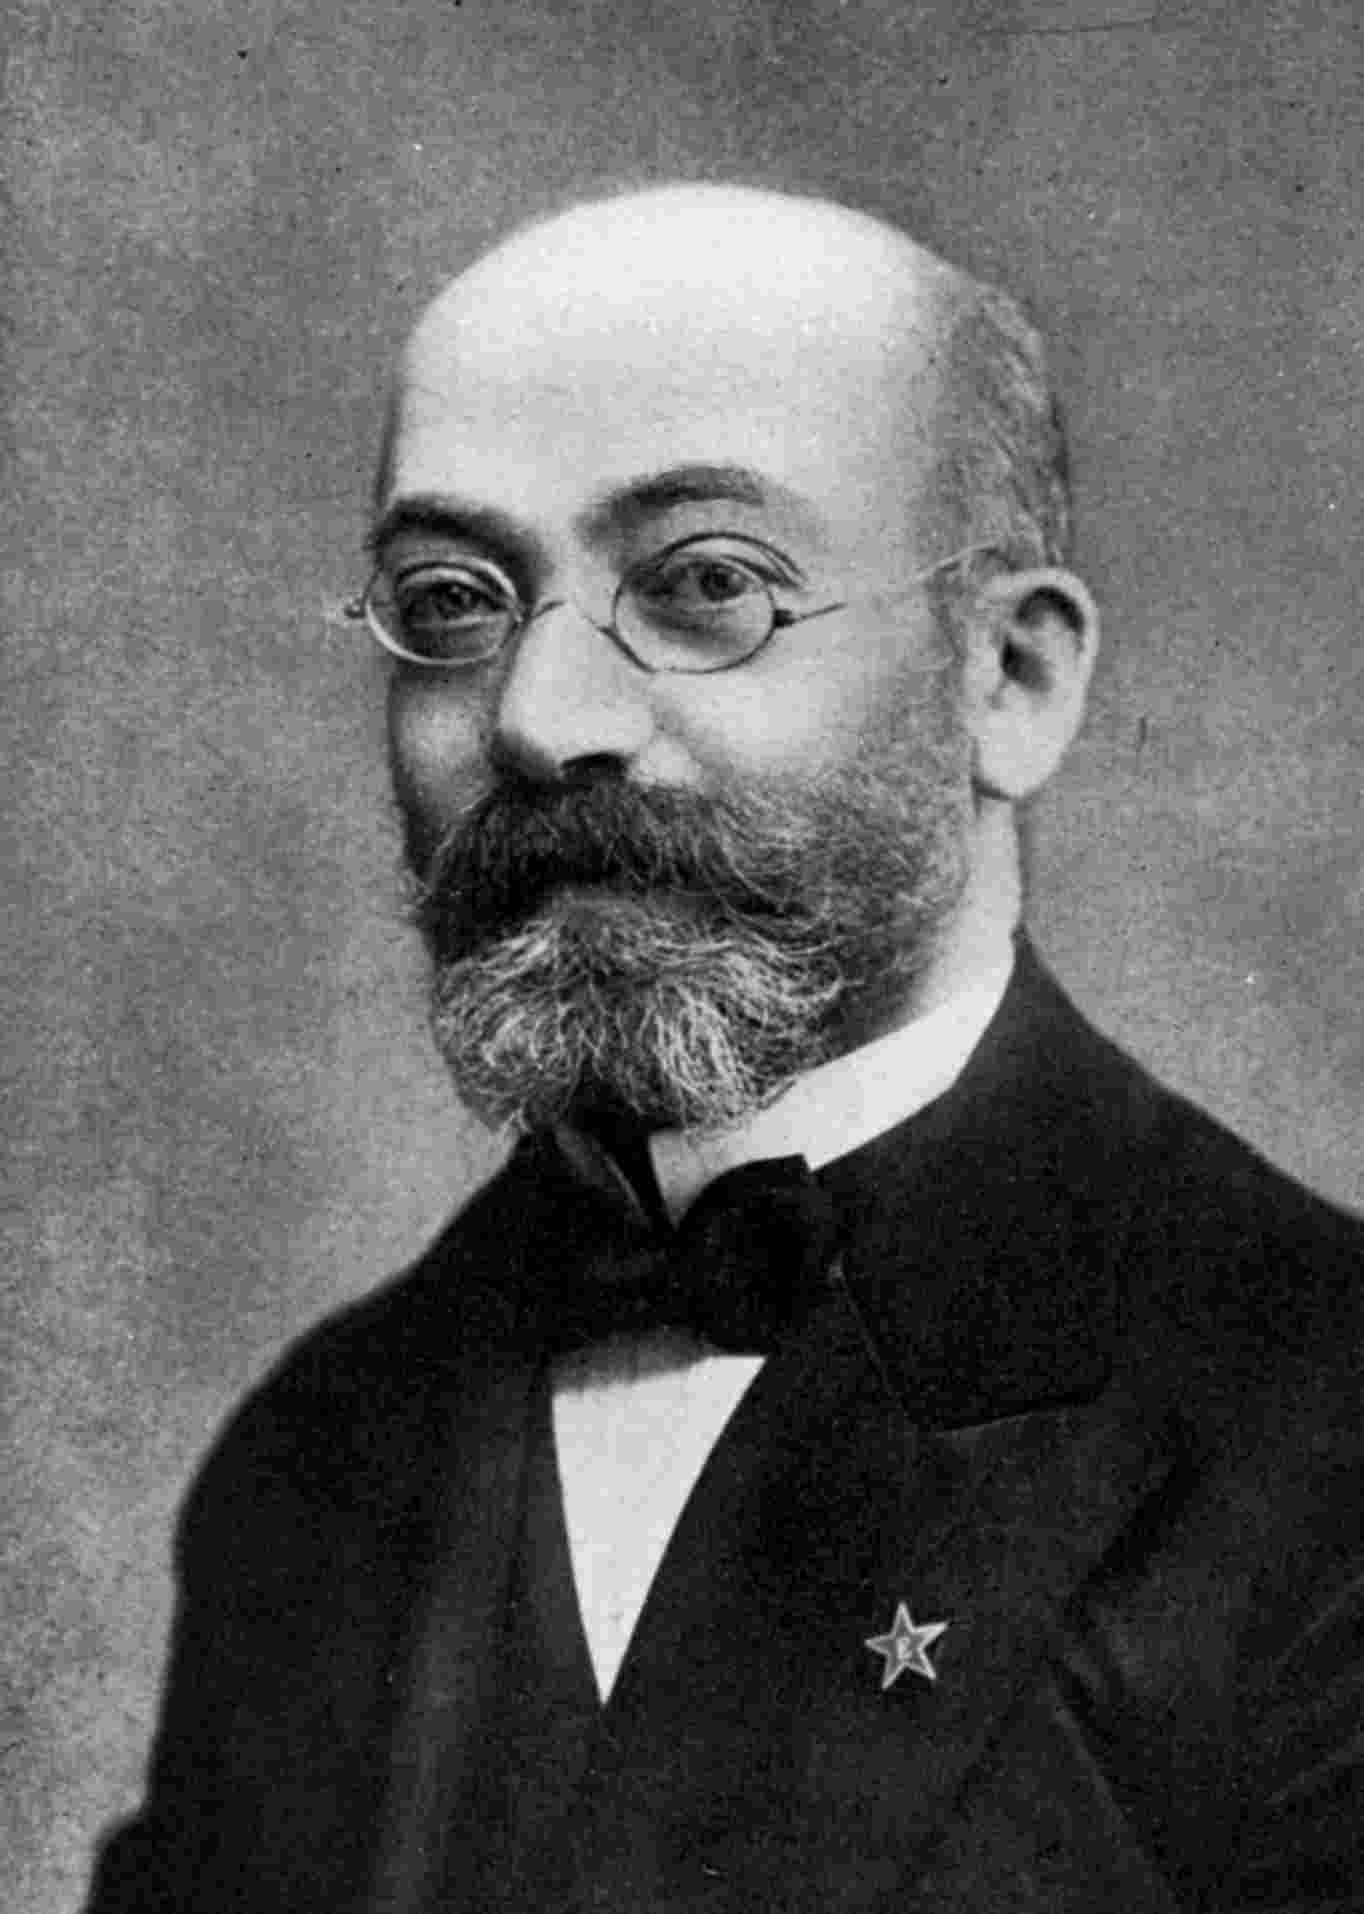
\includegraphics[scale=0.15]{../graphics/Zamenhof}
\end{figure}
\vspace*{0.5cm}
\nicefont
{\LARGE Lazaro Ludoviko ZAMENHOF} \\[1ex]
{\large Aŭtoro de la lingvo «Esperanto»} \\[1ex]
{\small (la 15-a de Decembro 1859 --- la 14-a de Aprilo 1917)}
 \vspace*{\stretch{1}}
\end{center}
\newpage
}

% Ligiloj, kaj ilia koloro 
%
\usepackage{color}
\definecolor{verda_ligilo}{rgb}{0,0.5,0}
\usepackage[colorlinks,linkcolor=verda_ligilo]{hyperref}
\usepackage{bookmark}

%
% Enkonduko por la Fundamenta Krestomatio
%

% ... kaj la libro estis presita de francoj
%
\usepackage{csquotes}
\DeclareQuoteStyle{esperanto}
  {\guillemotleft}{\guillemotright}
  {\guillemotleft}{\guillemotright}
\MakeOuterQuote{"}
\setquotestyle{esperanto}

% figuroj kaj matematiko (en la sunhorloĝa artikolo)
%
\usepackage{tikz}
\usetikzlibrary{shapes,arrows.meta}
\usepackage{amsmath}

% korespondantoj en "korespondado komerca"
%
\newcommand\koresp[1]{
\begin{flushleft}
\hspace{2em} #1
\end{flushleft}
}

% titoloj 
%
\renewcommand{\thechapter}{\Roman{chapter}}

% memoru:
% titleformat{command}[shape]{format}{label}{sep}{before-code}{after-code}
%
\titleformat{\chapter}[display]{\filcenter\Large}{\thechapter}{1ex}{\MakeUppercase}[{\rule{13mm}{0.4pt}}]
\titleformat{\section}[display]{\filcenter\large}{}{0pt}{\MakeUppercase}
\titlespacing{\section}{0pt}{1em}{1em}
\titleformat{\subsection}[display]{\filcenter\large}{}{0pt}{\MakeUppercase}

% citations
%
\newcommand\cited[1]{%
\begin{flushright}
\footnotesize #1
\end{flushright}}

\newcommand\citsc[1]{\cited{\fsc{#1}}}

% asterisms
%
%
%     *
%   *   *
\newcommand{\aster}{*} % maybe \ding{97} ?
\newcommand\asterism{
   \begin{center}
     \vspace{-1em}
     \parbox{1in}{ % needed to prevent split across page boundaries
       \begin{center}
         \aster\\
         \aster\hspace{0.6em}\aster
       \end{center}
     } %\parbox
     \vspace{-1em}
   \end{center}
 }

%
% reset footnote counter per page 
%
\usepackage{perpage} 
\MakePerPage{footnote} 

% parolanto, en Hamleto
%
\usepackage{ifthen}
\newcommand\speak[2][]{\makebox[0.7\textwidth]{\footnotesize {\ifthenelse{\equal{#1}{}}{\fsc{#2}}{#2}}}

\vspace*{-0.9em}

}

% spaco en Hamleto
%
\newlength{\xxx}
\newcommand\psp[1]{\settowidth{\xxx}{#1}\hspace{\xxx}}

% teatra direkto
%
\newcommand\stg[1]{\makebox[0.8\textwidth][r]{\footnotesize #1}}

% forigu la paĝnumero el la unua paĝo de ĉapitro
%
\fancypagestyle{plain}{%
  \renewcommand{\headrulewidth}{0pt}%
  \fancyhf{}%
}

% tabloj
%
\usepackage{longtable}
\usepackage{tabu}
\usepackage{siunitx}

% malgranda streko
%
\newcommand{\smallrule}{%
\begin{center}%
\rule{13mm}{0.4pt}\end{center}}

% La paĝtitoloj ŝanĝiĝas per ĉapitro, ne per sekcio aŭ subsekcio; do, 
% malpermesu al la (sub)sekcioj, ŝanĝi la paĝtitoloj
%
\renewcommand{\sectionmark}[1]{} 
\renewcommand{\subsectionmark}[1]{}

%
% Fino de Enkonduko
%


% versionombro
\newcommand{\laversio}{0.8}

%
% komenco
%
\begin{document}
\frontmatter

%
% plejeta ĉefpago
%
\vspace*{\fill}
\begin{center}
\nicefont
 {\LARGE FUNDAMENTA KRESTOMATIO}\\[0.8cm]
 {\large \spaceoutmed{DE LA LINGVO}}\\[0.8cm]
 {\scalebox{3}{\spaceout{ESPERANTO}}}
\end{center}
\vspace*{\fill}
\cleardoublepage

%
% ornama titolpaĝo
%
\thispagestyle{empty}
\begin{center}
 \begin{figure}[!ht]
 \centering 
\includegraphics[width=0.9\textwidth]{../graphics/terglobo.png}
 \end{figure}
 \nicefont
 
 {\large \spaceoutmed{L. ZAMENHOF}}

 \rule{13mm}{0.4pt}\\[1cm]

 {\LARGE FUNDAMENTA KRESTOMATIO}\\[0.8cm]
 {\spaceoutmed{DE LA LINGVO}}\\[0.8cm]
 {\scalebox{3}{\spaceout{ESPERANTO}}}

 \vspace*{\stretch{1}}

 \rule[0.5ex]{13mm}{0.4pt} \\
 {\small \spaceoutmed{DUA ELDONO}}\\
 \rule[0.7ex]{13mm}{0.4pt}

 \vspace*{\stretch{1}}

\csfont \footnotesize

\textsc{francujo.} — HACHETTE et C\textsuperscript{ie}, \textsc{\textit{paris.}}

\rule[0.9ex]{13mm}{0.4pt}

\textsc{anglujo.} – « REVIEW of REVIEWS », \textsc{\textit{london}}

\textsc{danujo.} — ANDR.-FRED. HÖST \& SÖN, \textsc{\textit{kjobenhavn.}}

\textsc{germanujo.} — MÖLLER \& BOREL, \textsc{\textit{berlin.}}

\textsc{hispanujo.} — J. ESPASA, \textsc{\textit{barcelona.}}

\textsc{italujo.} — RAFFAELO GIUSTI, \textsc{\textit{livorno.}}

\textsc{polujo.} — M. ARCT, \textsc{\textit{warszawa.}}

\textsc{svedujo.} — ESPERANTOFÖRENING, \textsc{\textit{stockholm.}}

\end{center}
 
\newpage

%
% D-ro Zamenhof
%
\zamenhof

%
% TOC (ho Dio ...)
%
\selectlanguage{esperanto}
\begin{center}
\narrow{\Large{TABELO DE LA ENHAVO}}
\thispagestyle{plain}
\end{center}

{ % environment for parskip settings

\setlength{\parindent}{0pt}
\setlength{\parskip}{1em}

{\centering \rule{13mm}{0.4pt}\par}

{\sansfont EKZERCOJ} \dotfill \pageref{ekzercoj}

{\centering \sansfont FABELOJ KAJ LEGENDOJ\par}

La novaj vestoj de la reĝo \dotfill \pageref{novajvestoj} \\
Aleksandro Macedona (V. Jabec) \dotfill \pageref{aleksandro} \\
Kiu estas la plej bona amiko de la viro? \dotfill \pageref{plejbona} \\
La deveno de la virino \dotfill \pageref{deveno} \\
La naskiĝo de la tabako (C. Bachiller) \dotfill \pageref{tabako}\\
Karagara \dotfill \pageref{karagara} \\
La virineto de maro \dotfill \pageref{virineto}

{\sansfont ANEKDOTOJ} \dotfill \pageref{anekdotoj}

{\centering \sansfont RAKONTOJ\par}

Nokto \dotfill \pageref{nokto} \\
La hejmo de la metiisto \dotfill \pageref{metiisto}\\
La forgesita pipo (A. Edelmann) \dotfill \pageref{pipo}\\
Arturo \dotfill \pageref{arturo}\\
La nigra virino \dotfill \pageref{nigra}\\
La karaj braceletoj \dotfill \pageref{braceletoj}\\
Nur unu vorton \dotfill \pageref{unuvorton}\\
La porcio da glaciaĵo \dotfill \pageref{porcio}

{\centering \sansfont EL LA VIVO KAJ SCIENCOJ\par}

Bagateloj \dotfill \pageref{bagateloj} \\
Fingra kalendaro \dotfill \pageref{fingra} \\
El la poŝto \dotfill \pageref{posxto} \\
La loĝejoj de la termitoj \dotfill \pageref{termitoj} \\
Korespondado komerca \dotfill \pageref{komerca} 

\newpage

Kronika katara konjunktivito \dotfill \pageref{kronika} \\
La sunhorloĝo en Dijon \dotfill \pageref{dijon} 

{\centering \sansfont ARTIKOLOJ PRI ESPERANTO\par}
\vspace{1em}

{ % outdent this section because the Leibnitz title is nuts

\setlength{\leftskip}{1em}
\setlength{\parindent}{-1em}
\setlength{\parskip}{0pt}

El la unua libro de la lingvo Esperanto \dotfill \pageref{unualibro}

Plena gramatiko de Esperanto  \dotfill \pageref{plena} 

Al la historio de la provoj de lingvoj tutmondaj de Leibnitz \\ ĝis la
  nuna tempo  \dotfill \pageref{leibnitz} 
  
Esenco kaj estonteco de la ideo de lingvo internacia  \dotfill \pageref{esenco} 

} % end outdented bit

{\centering \sansfont POEZIO\par}

% author, dash, poem, dots, page
\begin{longtabu} to\textwidth{@{}l@{ }c@{ }X@{}r@{}}
\bf L. Zamenhof. & --- & La espero \dotfill & \pageref{laespero}\\
\hfil--- & & La vojo \dotfill & \pageref{lavojo}\\
\hfil--- & & Al la fratoj \dotfill & \pageref{allafratoj}\\
\hfil--- & & Mia penso \dotfill & \pageref{miapenso}\\
\hfil--- & & Ho mia kor' \dotfill & \pageref{homiakor}\\
\hfil--- & & La vojevodo (Mickiewicz) \dotfill & \pageref{vojevodo}\\
\hfil--- & & La rozeto (Goethe) \dotfill & \pageref{rozeto}\\
\hfil--- & & En nord' unu pino (Heine) \dotfill & \pageref{unupino}\\
\hfil--- & & En sonĝo (Heine) \dotfill & \pageref{songxo}\\
\hfil--- & & Lorelej' (Heine) \dotfill & \pageref{lorelej}\\
\hfil--- & & Kanto de studentoj \dotfill & \pageref{studentoj}\\
\hfil--- & & Al la reĝo \dotfill & \pageref{regxo}\\
\hfil--- & & Nokta kanto de soldato (W. Hauff) \dotfill & \pageref{soldato}\\
\hfil--- & & Kanto de l'ligo (A. Mozart) \dotfill & \pageref{ligo}\\
\hfil--- & & La kapelo (L. Uhland) \dotfill & \pageref{kapelo}\\
\hfil--- & & La gaja migranto \dotfill & \pageref{migranto}\\
\hfil--- & & La vojo (B. N. Delvig) \dotfill & \pageref{lavojo2}\\
\vspace*{-38pt}
\end{longtabu}
\begin{longtabu} to\textwidth{@{}l@{ }c@{ }X@{}r@{}}
\bf Léo Belmont. &--- & Nokt' en la koro (Byron) \dotfill & \pageref{noktenlakoro}\\
\hfil--- & & Al brusto, al min (Heine) \dotfill & \pageref{albrusto}\\
\vspace*{-38pt}
\end{longtabu}
\begin{longtabu} to\textwidth{@{}l@{ }c@{ }X@{}r@{}}
\bf V. Devjatnin. & --- & Printempo \dotfill & \pageref{printempo}\\
\hfil--- & & Ŝipeto \dotfill & \pageref{sxipeto}\\
\hfil--- & & Sciuro kaj papago \dotfill & \pageref{sciuro}\\
\hfil--- & & Anĝelo (Lermontov) \dotfill & \pageref{angxelo}\\
\hfil---  &  & Husaro (Puŝkin) \dotfill & \pageref{husaro}\\
\bf V. Devjatnin. & --- & Infano de zorgo (Herder) \dotfill & \pageref{infano}\\
\hfil--- & & Espero (Schiller) \dotfill & \pageref{espero}\\
\hfil--- & & Garantio (Schiller) \dotfill & \pageref{garantio}\\
\vspace*{-38pt}
\end{longtabu}
\begin{longtabu} to\textwidth{@{}l@{ }c@{ }X@{}r@{}}
\bf A. Dombrowski. & --- & Mia mizero \dotfill & \pageref{mizero}\\
\hfil--- & & Nova kanto \dotfill & \pageref{nova}\\
\hfil--- & & La malliberulo \dotfill & \pageref{malliberulo}\\
\vspace*{-38pt}
\end{longtabu}
\begin{longtabu} to\textwidth{@{}l@{ }c@{ }X@{}r@{}}
\bf M. Goldberg. & --- & La turo babilona \dotfill & \pageref{turo}\\
\hfil--- & & Nova Dio (S. Frug) \dotfill & \pageref{novadio}\\
\hfil--- & & Cigno, ezoko kaj kankro (Krylov) \dotfill & \pageref{cigno}\\
\vspace*{-38pt}
\end{longtabu}
\begin{longtabu} to\textwidth{@{}l@{ }c@{ }X@{}r@{}}
\bf A. Grabowski. & --- & Tri Budrysoj (Mickiewicz) \dotfill & \pageref{tri}\\
\hfil--- & & Revaĵo (P. Dalman) \dotfill & \pageref{revajxo}\\
\hfil--- & & Excelsior (Longfellow) \dotfill & \pageref{excelsior}\\
\hfil--- & & La pluva tago (Longfellow) \dotfill & \pageref{pluva}\\
\hfil--- & & La sago kaj la kanto (Longfellow) \dotfill & \pageref{sago}\\
\hfil--- & & Sonoriloj de vespero (T. Moore) \dotfill & \pageref{sonoriloj}\\
\vspace*{-40pt}
\end{longtabu}
{\bf E. Haller.} --- Mi rakontis (Vejnberg) \dotfill  \pageref{rakontis}\\
{\bf G. Janowski.}  ---  Mi eliras (Lermontov) \dotfill \pageref{eliras}\\
{\bf D. Jegorov.}  ---  Aŭtuno \dotfill  \pageref{auxtuno}\\
{\bf F. de Kanaloŝŝy-Lefler.}  ---  Kuŝas somero (Heine) \dotfill  \pageref{somero}\\
\vspace*{-21pt}
\begin{longtabu} to\textwidth{@{}l@{ }c@{ }X@{}r@{}}
\bf A. Kofman. & --- & Filino de Iftah \dotfill & \pageref{filino}\\
\hfil--- & & La sklavoŝipo (Heine) \dotfill & \pageref{sklavo}\\
\vspace*{-40pt}
\end{longtabu}
{\bf V. Langlet.} --- Al la memoro de Jozef Wasniewski \dotfill \pageref{memoro}\\
{\bf R. Libeks.}  ---  Latva popola kanto \dotfill  \pageref{latva}\\
\vspace*{-21pt}
\begin{longtabu} to\textwidth{@{}l@{ }c@{ }X@{}r@{}}
\bf I. Lojko & --- & Malgrand'-rusa kanteto \dotfill & \pageref{malgrand}\\
\hfil--- & & Profeto (Lermontov) \dotfill & \pageref{profeto}\\
\vspace*{-40pt}
\end{longtabu}
{\bf F. Lorenc.}  ---  Alaŭdeto (Boheme) \dotfill  \pageref{alauxdeto}\\
\vspace*{-21pt}
\begin{longtabu} to\textwidth{@{}l@{ }c@{ }X@{}r@{}}
\bf A. Naumann. & --- & Mi amis vin \dotfill & \pageref{miamasvin}\\
\hfil--- & & Printempo venos \dotfill & \pageref{printempovenos}\\
\vspace*{-40pt}
\end{longtabu}
{\bf Poeteto.}  ---  La Ĉaso \dotfill  \pageref{cxaso}\\
\vspace*{-21pt}
\begin{longtabu} to\textwidth{@{}l@{ }c@{ }X@{}r@{}}
\bf I. Seleznet. & --- & Kanto. \dotfill & \pageref{kanto}\\
\hfil--- & & Ne riproĉu la sorton \dotfill & \pageref{riprocxu}\\
\hfil--- & & Revo \dotfill & \pageref{revo}\\
\vspace*{-40pt}
\end{longtabu}
{\bf E. Smetanka.}  ---  La poeto (V. Halek) \dotfill  \pageref{poeto}\\
{\bf L. Sokolov.}  ---  La velo (Lermontov) \dotfill  \pageref{velo}\\

\newpage
\begin{longtabu} to\textwidth{@{}l@{ }c@{ }X@{}r@{}}
\bf M. Solovjev. & --- & Plendo \dotfill & \pageref{plendo}\\
\hfil--- & & Tri palmoj (Lermontov) \dotfill & \pageref{palmoj}\\
\vspace*{-40pt}
\end{longtabu}
{\bf K. Svanbom.}  ---  Laŭ sveda melodio \dotfill  \pageref{sveda}\\
{\bf S. Satunovski.}  ---  Ne diru (Nadson) \dotfill  \pageref{nediru}\\
{\bf W. Waher.}  ---  Spirita Ŝipo \dotfill  \pageref{spirita}\\
{\bf J. Wasniewski.}  --- El la paperujo de miaj fabloj \dotfill  \pageref{paperujo}\\
{\bf E. de Wahl.}  ---  Ĉe l' maro (Heine) \dotfill  \pageref{maro}\\
\vspace*{-21pt}
\begin{longtabu} to\textwidth{@{}l@{ }c@{ }X@{}r@{}}
\bf F. Zamenhof. & --- & Versaĵo sen fino \dotfill \pageref{senfino}\\
\hfil--- & & Vizito de la steloj sur la tero \dotfill \pageref{vizito}\\
\vspace*{-40pt}
\end{longtabu}
{\bf O. Zeidlitz.}  ---  Vespero (A. Nikander) \dotfill  \pageref{vespero}\\
{\bf L. Zamenhof.}  ---  El Hamleto \dotfill  \pageref{hamleto}\\
{\bf A. Kofman.} --- El Iliado \dotfill  \pageref{iliado}

{\centering \sansfont ALDONO\par}

Preĝo sub la verda standardo \dotfill \pageref{standardo}

} % end environment for parskip settings

\vspace*{\fill}

\begin{center}
\rule{13mm}{0.4pt}\\
\footnotesize 1432-05. --- Coulommiers. Imp. \fsc{Paul} BRODARD. --- 12-05.
\end{center}
\cleardoublepage



 Antaŭparolo

\chapter*{Anta\u uparolo}
\thispagestyle{empty}
\fancyhead[LE,RO]{\footnotesize\thepage}
\fancyhead[CE]{\footnotesize\leftmark}
\fancyhead[CO]{\footnotesize\rightmark}
\markboth{FUNDAMENTA KRESTOMATIO.}{ANTAŬPAROLO.}
\label{antau}
Prezentante pure kondi\^can rimedon de reciproka komuniki\^gado, la
lingvo internacia, simile al \^ciu lingvo nacia, povos bone atingi
sian celon nur en tiu okazo, se \^ciuj uzos \^gin plene {\it egale};
kaj por ke \^ciuj povu uzi la lingvon egale, estas necese, ke
ekzistu iaj {\it modeloj}, le\^gdonaj por \^ciuj. Tio \^ci estas la
ka\u uzo, pro kiu, cedante al la peto de multaj esperantistoj, mi
eldonis la {\it Fundamentan Krestomation}, kiu povos servi al \^ciuj
kiel modelo de esperanta stilo kaj gardi la lingvon de pereiga
disfalo je diversaj dialektoj.

   Lerni la lingvon \^ciu povas la\u u \^ciuj libroj, kiujn li deziros; sed
\^car multaj esperantaj libroj estas verkitaj de personoj, kiuj
ankora\u u ne posedas bone la lingvon Esperanto, kaj komencanta
esperantisto ne povus rilati al ili sufi\^ce kritike, tial estas
dezirinde, ke \^ciu, anta\u u ol komenci la legadon de la esperanta
literaturo, tralegu atente la {\it Fundamentan Krestomation}. Ne
deprenante de la lernanto la eblon kritike proprigi al si \^ciujn
ri\^cigojn kaj regule faritajn perfektigojn, kiujn li trovas en la
literaturo, la {\it Fundamenta Krestomatio} por \^ciam gardos lin de
blinda kaj senkritika alproprigo de stilo {\it erara}.

   Atentan tralegon de la {\it Fundamenta Krestomatio} mi rekomendas al
{\it \^ciu}, kiu volas skribe a\u u parole uzi la lingvon Esperanto.
{\it Sed precipe atentan kaj kelkfojan trategon de tiu \^ci libro mi
rekomendas al tiuj, kiuj deziras eldoni verkojn en Esperanto}; \^car
tiu, kiu eldonas verkon en Esperanto, ne koni\^ginte anta\u ue
fundamente kun la spirito kaj la modela stilo de tiu \^ci lingvo,
alportas al nia afero ne utilon, sed rektan malutilon.

   \^Ciuj artikoloj en la {\it Fundamenta Krestomatio} estas a\u u skribitaj
de mi mem, a\u u --- se ili estas skribitaj de aliaj personoj ---
ili estas korektitaj de mi en tia grado, ke la stilo en ili ne
deflanki\^gu de la stilo, kiun mi mem uzas.

\begin{flushright}
\begin{minipage}{5cm}
\begin{center}
L. \fsc{Zamenhof},\\
\footnotesize A\u utoro de la lingvo {\it Esperanto}.
\end{center}
\end{minipage}
\end{flushright}
\begin{flushleft}
\small Varsovio, en Aprilo 1903.
\end{flushleft}



 Ekzercoj

\mainmatter
\titleformat{\chapter}[display]{\filcenter\Large}{\vspace*{-4em}\narrow{\huge{\textbf{FUNDAMENTA KRESTOMATIO}}}\\\rule{\textwidth}{0.4pt}\\[2cm]\thechapter}{1ex}{\MakeUppercase}[{\rule{13mm}{0.4pt}}]
\chapter{Ekzercoj}
\markboth{FUNDAMENTA KRESTOMATIO.}{EKZERCOJ.}
\label{ekzercoj}
\section*{\S\,1.}
Patro kaj frato. --- Leono estas besto. --- Rozo estas floro, kaj
kolombo estas birdo. --- La rozo apartenas al Teodoro. --- La suno
brilas. --- La patro estas sana. --- La patro estas tajloro.

\section*{\S\,2.}
Infano ne estas matura homo. --- La infano jam ne ploras. --- La
\^cielo estas blua. --- Kie estas la libro kaj la krajono? --- La
libro estas sur la tablo, kaj la krajono ku\^sas sur la fenestro.
--- Sur la fenestro ku\^sas krajono kaj plumo. --- Jen estas
pomo. --- Jen estas la pomo, kiun mi trovis. --- Sur la tero ku\^sas
\^stono.


\section*{\S\,3.}
Leono estas forta. --- La dentoj de leono estas akraj. --- Al leono
ne donu la manon. --- Mi vidas leonon. --- Resti kun leono estas
dan\^gere. --- Kiu kura\^gas rajdi sur leono? --- Mi parolas pri
leono.


\section*{\S\,4.}
La patro estas bona. --- Jen ku\^sas la \^capelo de la patro. ---
Diru al la patro, ke mi estas diligenta. --- Mi amas la patron. ---
Venu kune kun la patro. --- La filo staras apud la patro. --- La
mano de Johano estas pura. --- Mi konas Johanon. --- Ludoviko, donu
al mi panon. --- Mi man\^gas per la bu\^so kaj flaras per la nazo.
--- Anta\u u la domo staras arbo. --- La patro estas en la \^cambro.


\section*{\S\,5.}
La birdoj flugas.--- La kanto de la birdoj estas agrabla.--- Donu al
la birdoj akvon, \^car ili volas trinki. --- La knabo forpelis la
birdojn. --- Ni vidas per la okuloj kaj a\u udas perla oreloj.
--- Bonaj infanoj lernas diligente. --- Aleksandro ne volas lerni, kaj
tial mi batas Aleksandron. --- De la patro mi ricevis libron, kaj de
la frato mi ricevis plumon. --- Mi venas de la avo; kaj mi iras nun
al la onklo. --- Mi legas libron. --- La patro ne legas libron, sed
li skribas leteron.

\enlargethispage{-\baselineskip}
\section*{\S\,6.}
Papero estas blanka. --- Blanka papero ku\^sas sur la tablo. --- La
blanka papero jam ne ku\^sas sur la tablo. --- Jen estas la kajero
de la juna fra\u ulino. --- La patro donis al mi dol\^can pomon. ---
Rakontu al mia juna amiko belan historion. --- Mi ne amas obstinajn
homojn. --- Mi deziras al vi bonan tagon, sinjoro! --- Bonan
matenon! --- \^Gojan feston! (mi deziras al vi). --- Kia \^goja
festo! (estas hodia\u u). --- Sur la \^cielo staras la bela suno.
--- En la tago ni vidas la helan sunon, kaj en la nokto ni vidas la
palan lunon kaj la belajn stelojn. --- La papero estas tre blanka,
sed la ne\^go estas pli blanka. --- Lakto estas pli nutra, ol vino.
--- Mi havas pli fre\^san panon, ol vi. --- Ne, vi eraras, sinjoro:
via pano estas malpli fre\^sa, ol mia. --- El \^ciuj miaj infanoj
Ernesto estas la plej juna. --- Mi estas tiel forta, kiel vi. --- El
\^ciuj siaj fratoj Antono estas la malplej sa\^ga.

\section*{\S\,7.}
Du homoj povas pli multe fari ol unu. --- Mi havas nur unu bu\^son,
sed mi havas du orelojn. --- Li promenas kun tri hundoj. --- Li
faris \^cion per la dek fingroj de siaj manoj. --- El \^siaj multaj
infanoj unuj estas bonaj kaj aliaj estas malbonaj. --- Kvin kaj sep
faras dek du. --- Dek kaj dek faras dudek. --- Kvar kaj dek ok faras
dudek du. --- Tridek kaj kvardek kvin faras sepdek kvin. --- Mil
okcent na\u udek tri. --- Li havas dek unu infanojn. --- Sesdek
minutoj faras unu horon, kaj unu minuto konsistas el sesdek
sekundoj. --- Januaro estas la unua monato de la jaro, Aprilo estas
la kvara, Novembro estas la dek-unua, Decembro estas la dek-dua.
--- La dudeka (tago) de Februaro estas la kvindek-unua tago de la
jaro. --- La sepan tagon de la semajno Dio elektis, ke \^gi estu pli
sankta, ol la ses unuaj tagoj. --- Kion Dio kreis en la sesa tago?
--- Kiun daton ni havas hodia\u u? --- Hodia\u u estas la dudek sepa
(tago) de Marto. --- Georgo Va\^sington estis naskita la dudek duan
de Februaro de la jaro mil sepcent tridek dua.


\section*{\S\,8.}
Mi havas cent pomojn. --- Mi havas centon da pomoj. --- Tiu \^ci
urbo havas milionon da lo\^gantoj. --- Mi a\^cetis dekduon (a\u u
dek-duon) da kuleroj kaj du dekduojn da forkoj. --- Mil jaroj (a\u u
milo da jaroj) faras miljaron. --- Unue mi redonas al vi la monon,
kiun vi pruntis al mi; due mi dankas vin por la prunto; trie mi
petas vin anka\u u poste prunti al mi, kiam mi bezonos monon. ---
Por \^ciu tago mi ricevas kvin frankojn, sed por la hodia\u ua tago
mi ricevis duoblan pagon, t. e. (= tio estas) dek frankojn.
--- Kvinoble sep estas tridek kvin. --- Tri estas duono de ses. --- Ok
estas kvar kvinonoj de dek. --- Kvar metroj da tiu \^ci \^stofo
kostas na\u u frankojn; tial du metroj kostas kvar kaj duonon
frankojn (a\u u da frankoj). --- Unu tago estas
tricent-sesdek-kvinono a\u u tricent-sesdek-sesono de jaro. --- Tiuj
\^ci du amikoj promenas \^ciam duope. --- Kvinope ili sin \^{\j}etis
sur min, sed mi venkis \^ciujn kvin atakantojn. --- Por miaj kvar
infanoj mi a\^cetis dek du pomojn, kaj al \^ciu el la infanoj mi
donis po tri pomoj. --- Tiu \^ci libro havas sesdek pa\^gojn; tial,
se mi legos en \^ciu tago po dek kvin pa\^goj, mi finos la tutan
libron en kvar tagoj.


\section*{\S\,9.}
 Mi legas. --- Ci skribas (anstata\u u "ci" oni uzas ordinare "vi"),
 --- Li estas knabo, kaj \^si estas knabino. --- La tran\^cilo tran\^cas
bone, \^car \^gi estas akra. --- Ni estas homoj. --- Vi estas
infanoj. --- Ili estas rusoj. --- Kie estas la knaboj? --- Ili estas
en la \^gardeno. --- Kie estas la knabinoj? --- Ili anka\u u estas
en la \^gardeno. --- Kie estas la tran\^ciloj? --- Ili ku\^sas sur
la tablo. --- Mi vokas la knabon, kaj li venas. --- Mi vokas la
knabinon, kaj \^si venas. --- La infano ploras, \^car \^gi volas
man\^gi. --- La infanoj ploras, \^car ili volas man\^gi. --- Knabo,
vi estas ne\^gentila. --- Sinjoro, vi estas ne\^gentila.
--- Sinjoroj, vi estas ne\^gentilaj. --- Mia hundo, vi estas tre
fidela. --- Oni diras, ke la vero \^ciam venkas. --- En la vintro
oni hejtas la fornojn. --- Kiam oni estas ri\^ca (a\u u ri\^caj),
oni havas multajn amikojn.

\section*{\S\,10.}
Li amas min, sed mi lin ne amas. --- Mi volis lin bati, sed li
forkuris de mi. --- Diru al mi vian nomon. --- Ne skribu al mi tiajn
longajn leterojn. --- Venu al mi hodia\u u vespere. --- Mi rakontos
al vi historion. --- \^Cu vi diros al mi la veron? --- La domo
apartenas al li. --- Li estas mia onklo, \^car mia patro estas lia
frato. --- Sinjoro Petro kaj lia edzino tre amas miajn infanojn; mi
anka\u u tre amas (infanojn). --- Montru al ili vian novan veston.
--- Mi amas min mem, vi amas vin mem, li amas sin mem, kaj \^ciu
homo amas sin mem. --- Mia frato diris al Stefano, ke li amas lin
pli, ol sin mem. --- Mi zorgas pri \^si tiel, kiel mi zorgas pri mi
mem; sed \^si mem tute ne zorgas pri si kaj tute sin ne gardas.
--- Miaj fratoj havis hodia\u u gastojn; post la vesperman\^go niaj
fratoj eliris kun la gastoj el sia domo kaj akompanis ilin \^gis
ilia domo. --- Mi jam havas mian \^capelon; nun ser\^cu vi vian.
--- Mi lavis min en mia \^cambro, kaj \^si lavis sin en sia
\^cambro. --- La infano ser\^cis sian pupon; mi montris al la
infano, kie ku\^sas \^gia pupo. --- Oni ne forgesas facile sian
unuan amon.

\section*{\S\,11.}
Nun mi legas, vi legas kaj li legas; ni \^ciuj legas. --- Vi
skribas, kaj la infanoj skribas; ili \^ciuj sidas silente kaj
skribas. --- Hiera\u u mi renkontis vian filon, kaj li \^gentile
salutis min. --- Hodia\u u estas sabato, kaj morga\u u estos
diman\^co. --- Hiera\u u estis vendredo, kaj post-morga\u u estos
lundo. --- Anta\u u tri tagoj mi vizitis vian kuzon kaj mia vizito
faris al li plezuron. --- \^Cu vi jam trovis vian horlo\^gon? --- Mi
\^gin ankora\u u ne ser\^cis; kiam mi finos mian laboron, mi
ser\^cos mian horlo\^gon, sed mi timas, ke mi \^gin jam ne trovos.
--- Kiam mi venis al li, li dormis; sed mi lin vekis. --- Se mi estus
sana, mi estus feli\^ca. --- Se li scius, ke mi estas tie \^ci, li
tuj venus al mi. --- Se la lernanto scius bone sian lecionon, la
instruanto lin ne punus. --- Kial vi ne respondas al mi? \^Cu vi
estas surda a\u u muta? --- Iru for! --- Infano, ne tu\^su la
spegulon! --- Karaj infanoj, estu \^ciam honestaj! --- Li venu, kaj
mi pardonos al li. --- Ordonu al li, ke li ne babilu. --- Petu
\^sin, ke \^si sendu al mi kandelon. --- Ni estu gajaj, ni uzu bone
la vivon, \^car la vivo ne estas longa. --- \^Si volas danci. Morti
pro la patrujo estas agrable. --- La infano ne \^cesas petoli.

\section*{\S\,12.}
Fluanta akvo estas pli pura, ol akvo, staranta senmove.
--- Promenante sur la strato, mi falis. --- Kiam Nikodemo batas
Jozefon, tiam Nikodemo estas la batanto kaj Jozefo estas la batato.
--- Al homo, pekinta senintence, Dio facile pardonas. --- Trovinte
pomon, mi \^gin man\^gis. --- La falinta homo ne povis sin levi. ---
Ne ripro\^cu vian amikon, \^car vi mem pli multe meritas ripro\^con;
li estas nur unufoja mensoginto, dum vi estas ankora\u u nun \^ciam
mensoganto. --- La tempo pasinta jam neniam revenos; la tempon
venontan neniu ankora\u u konas. --- Venu, ni atendas vin, Savonto
de la mondo. --- En la lingvo "Esperanto" ni vidas la estontan
lingvon helpantan de la tuta mondo. --- A\u ugusto estas mia plej
amata filo. --- Mono havata estas pli grava ol havita. --- Pasero
kaptita estas pli bona, ol aglo kaptota. --- La soldatoj kondukis la
arestitojn tra la stratoj. --- Li venis al mi tute ne atendite.
--- Homo, kim oni devas ju\^gi, estas ju\^goto.

\section*{\S\,13.}
Nun li diras al mi la veron. --- Hiera\u u li diris al mi la veron.
--- Li \^ciam diradis al mi la veron. --- Kiam vi vidis nin en la
salono, li jam anta\u ue diris al mi la veron (a\u u li estis
dirinta al mi la veron). --- Li diros al mi la veron. --- Kiam vi
venos al mi, li jam anta\u ue diros al mi la veron (a\u u li estos
dirinta al mi la veron; a\u u anta\u u ol vi venos al mi, li diros
al mi la veron). --- Se mi petus lin, li dirus al mi la veron. ---
Mi ne farus la eraron, se li anta\u ue dirus al mi la veron (a\u u
se li estus dirinta al mi la veron). --- Kiam mi venos, diru al mi
la veron. --- Kiam mia patro venos, diru al mi anta\u ue la veron
(a\u u estu dirinta al mi la veron). --- Mi volas diri al vi la
veron. --- Mi volas, ke tio, kion mi diris, estu vera (a\u u mi
volas esti dirinta la veron).

\section*{\S\,14.}
Mi estas amata. Mi estis amata. Mi estos amata. Mi estus amata. Estu
amata. Esti amata. --- Vi estas lavita. Vi estis lavita. Vi estos
lavita. Vi estus lavita. Estu lavita. Esti lavita. --- Li estas
invitota. Li estis invitota. Li estos invitota. Li estus invitota.
Estu invitota. Esti invitota. --- Tiu \^ci komerca\^{\j}o estas
\^ciam volonte a\^cetata de mi. --- La surtuto estas a\^cetita de
mi, sekve \^gi apartenas al mi. --- Kiam via domo estis konstruata,
mia domo estis jam longe konstruita. --- Mi sciigas, ke de nun la
\^suldoj de mia filo ne estos pagataj de mi. --- Estu trankvila, mia
tuta \^suldo estos pagita al vi balda\u u. --- Mia ora ringo ne
estus nun tiel longe ser\^cata, se \^gi ne estus tiel lerte ka\^sita
de vi. --- La\u u la projekto de la in\^genieroj tiu \^ci fervojo
estas konstruota en la da\u uro de du jaroj; sed mi pensas, ke \^gi
estos konstruata pli ol tri jarojn. --- Honesta homo agas honeste.
--- La pastro, kiu mortis anta\u u nelonge (a\u u anta\u u nelonga
tempo), lo\^gis longe en nia urbo. --- \^Cu hodia\u u estas varme
a\u u malvarme? --- Sur la kameno inter du potoj staras fera
kaldrono; el la kaldrono, en kiu sin trovas bolanta akvo, eliras
vaporo; tra la fenestro, kiu sin trovas apud la pordo, la vaporo
iras sur la korton.

\section*{\S\,15.}
Kie vi estas? --- Mi estas en la \^gardeno. --- Kien vi iras? --- Mi
iras en la \^gardenon. --- La birdo flugas en la \^cambro (--- \^gi
estas en la \^cambro kaj flugas en \^gi). --- La birdo flugas en la
\^cambron (--- \^gi estas ekster la \^cambro kaj flugas nun en
\^gin). --- Mi voja\^gas en Hispanujo. --- Mi voja\^gas en
Hispanujon. --- Mi sidas sur se\^go kaj tenas la piedojn sur
benketo. --- Mi metis la manon sur la tablon. El sub la kanapo la
muso kuris sub la liton, kaj nun \^gi kuras sub la lito. --- Super
la tero sin trovas aero. --- Anstata\u u kafo li donis al mi teon
kun sukero, sed sen kremo. --- Mi staras ekster la domo, kaj li
estas interne. --- En la salono estis neniu krom li kaj lia
fian\^cino. --- La hirundo flugis trans la riveron, \^car trans la
rivero sin trovis aliaj hirundoj. --- Mi restas tie \^ci la\u u la
ordono de mia estro. --- Kiam li estis \^ce mi, li staris tutan
horon apud la fenestro. --- Li diras, ke mi estas atenta. --- Li
petas, ke mi estu atenta. --- Kvankam vi estas ri\^ca, mi dubas,
\^cu vi estas feli\^ca. --- Se vi scius, kiu li estas, vi lin pli
estimus. --- Se li jam venis, petu lin al mi. --- Ho, Dio! kion vi
faras! --- Ha, kiel bele! --- For de tie \^ci! --- Fi, kiel abomene!
--- Nu, iru pli rapide!

\section*{\S\,16.}
La artikolo "la" estas uzata tiam, kiam ni parolas pri personoj
a\u u objektoj konataj. \^Gia uzado estas tia sama, kiel en la aliaj
lingvoj. La personoj, kiuj ne komprenas la uzadon de la artikolo
(ekzemple rusoj a\u u poloj, kiuj ne scias alian lingvon krom sia
propra), povas en la unua tempo tute ne uzi la artikolon, \^car \^gi
estas oportuna, sed ne necesa. Anstata\u u "la" oni povas anka\u u
diri "l"' (sed nur post prepozicio, kiu fini\^gas per vokalo).
--- Vortoj kunmetitaj estas kreataj per simpla kunligado de vortoj;
oni prenas ordinare la purajn radikojn, sed, se la bonsoneco a\u u
la klareco postulas, oni povas anka\u u preni la tutan vorton, t. e.
la radikon kune kun \^gia gramatika fini\^go. Ekzemploj: skribtablo
a\u u skribotablo (= tablo, sur kiu oni skribas); internacia (= kiu
estas inter diversaj nacioj); tutmonda (= de la tuta mondo); unutaga
(= kiu da\u uras unu tagon); unuataga (= kiu estas en la unua tago);
vapor\^sipo (= \^sipo, kiu sin movas per vaporo); matenman\^gi,
tagman\^gi, vesperman\^gi; abonpago (= pago por la abono).


\section*{\S\,17.}
\^Ciuj prepozicioj per si mem postulas \^ciam nur la nominativon. Se
ni iam post propozicio uzas la akuzativon, la akuzativo tie dependas
ne de la prepozicio, sed de aliaj ka\u uzoj. Ekzemple: por esprimi
direkton, ni aldonas al la vorto la finon "n" ; sekve: tie (= en
tiu loko), tien (= al tiu loko); tiel same ni anka\u u diras: "la
birdo flugis en la \^gardenon, sur la tablon", kaj la vortoj
"\^gardenon", "tablon" staras tie \^ci en akuzativo ne \^car la
prepozicioj "en" kaj "sur" tion \^ci postulas, sed nur \^car ni
volis esprimi direkton, t. e. montri, ke la birdo sin ne trovis
anta\u ue en la \^gardeno a\u u sur la tablo kaj tie flugis, sed ke
\^gi de alia loko flugis al la \^gardeno, al la tablo (ni volas
montri, ke la \^gardeno kaj tablo ne estis la loko de la flugado,
sed nur la celo de la flugado); en tiaj okazoj ni uzus la fini\^gon
"n" tute egale, \^cu ia prepozicio starus a\u u ne. --- Morga\u u
mi veturos Parizon (a\u u en Parizon). --- Mi restos hodia\u u dome.
--- Jam estas tempo iri domen. --- Ni disi\^gis kaj iris en
diversajn flankojn: mi iris dekstren, kaj li iris maldekstren. ---
Flanken, sinjoro! Mi konas neniun en tiu \^ci urbo. --- Mi neniel
povas kompreni, kion vi parolas. --- Mi renkontis nek lin, nek lian
fraton (a\u u mi ne renkontis lin, nek lian fraton).


\section*{\S\,18.}
Se ni bezonas uzi prepozicion kaj la senco ne montras al ni, kian
prepozicion uzi, tiam ni povas uzi la komunan prepozicion "je".
Sed estas bone uzadi la vorton "je" kiel eble pli malofte.
Anstata\u u la vorto "je" ni povas anka\u u uzi akuzativon sen
prepozicio.
--- Mi ridas je lia naiveco (a\u u mi ridas pro lia naiveco, a\u u:
mi ridas lian naivecon). --- Je la lasta fojo mi vidis lin \^ce vi
(a\u u: la lastan fojon). --- Mi veturis du tagojn kaj unu nokton.
--- Mi sopiras je mia perdita feli\^co (a\u u: mian perditan
feli\^con).
--- El la dirita regulo sekvas, ke se ni pri ia verbo ne scias, \^cu
\^gi postulas post si la akuzativon (t. e. \^cu \^gi estas aktiva)
a\u u ne, ni povas \^ciam uzi la akuzativon. Ekzemple, ni povas diri
"obei al la patro" kaj "obei la patron" (anstata\u u "obei je
la patro"). Sed ni ne uzas la akuzativon tiam, kiam la klareco de
la senco tion \^ci malpermesas; ekzemple: ni povas diri "pardoni al
la malamiko" kaj "pardoni la malamikon", sed ni devas diri \^ciam
"pardoni al la malamiko lian kulpon".


\section*{\S\,19.}
Ia, ial, iam, ie, iel, ies, io, iom, iu. --- La montritajn na\u u
vortojn ni konsilas bone ellerni, \^car el ili \^ciu povas jam fari
al si grandan serion da aliaj pronomoj kaj adverboj. Se ni aldonas
al ili la literon "k", ni ricevas vortojn demandajn a\u u
rilatajn: kia, kial, kiam, kie, kiel, kies, kio, kiom, kiu. Se ni
aldonas la literon "t", ni ricevas vortojn montrajn: tia, tial,
tiam, tie, tiel, ties, tio, tiom, tiu. Aldonante la literon "\^c",
ni ricevas vortojn komunajn: \^cia, \^cial, \^ciam, \^cie, \^ciel,
\^cies, \^cio, \^ciom, \^ciu. Aldonante la prefikson "nen", ni
ricevas vortojn neajn: nenia, nenial, neniam, nenie, neniel, nenies,
nenio, neniom, neniu. Aldonante al la vortoj montraj la vorton
"\^ci", ni ricevas montron pli proksiman; ekzemple: tiu (pli
malproksima), tiu \^ci (a\u u \^ci tiu) (pli proksima); tie
(malproksime), tie \^ci a\u u \^ci tie (proksime). Aldonante al la
vortoj demandaj la vorton "ajn", ni ricevas vortojn
sendiferencajn: kia ajn, kial ajn, kiam ajn, kie ajn, kiel ajn, kies
ajn, kio ajn, kiom ajn, kiu ajn. Ekster tio el la diritaj vortoj ni
povas ankora\u u fari aliajn vortojn, per helpo de gramatikaj
fini\^goj kaj aliaj vortoj (sufiksoj); ekzemple: tiama, \^ciama,
kioma, tiea, \^ci-tiea, tieulo, tiamulo k. t. p. (= kaj tiel plu).


\section*{\S\,20.}
Lia kolero longe da\u uris. --- Li estas hodia\u u en kolera humoro.
--- Li koleras kaj insultas. --- Li fermis kolere la pordon. --- Lia
filo mortis kaj estas nun malviva. --- La korpo estas morta, la
animo estas senmorta. --- Li estas morte malsana, li ne vivos pli,
ol unu tagon. --- Li parolas, kaj lia parolo fluas dol\^ce kaj
agrable. --- Ni faris la kontrakton ne skribe, sed parole. --- Li
estas bona parolanto. --- Starante ekstere, li povis vidi nur la
eksteran flankon de nia domo. --- Li lo\^gas ekster la urbo. --- La
ekstero de tiu \^ci homo estas pli bona, ol lia interno. --- Li tuj
faris, kion mi volis, kaj mi dankis lin por la tuja plenumo de mia
deziro. --- Kia granda brulo! kio brulas? --- Ligno estas bona brula
materialo. --- La fera bastono, kiu ku\^sis en la forno, estas nun
brule varmega. --- \^Cu li donis al vi jesan respondon a\u u nean?
Li eliris el la dormo\^cambro kaj eniris en la man\^go\^cambron.
--- La birdo ne forflugis: \^gi nur deflugis de la arbo, alflugis al
la domo kaj surflugis sur la tegmenton. --- Por \^ciu a\^cetita
funto da teo tiu \^ci komercisto aldonas senpage funton da sukero.
--- Lernolibron oni devas ne trale\^gi, sed tralerni. --- Li portas
rozokoloran superveston kaj teleroforman \^capelon. --- En mia
skribotablo sin trovas kvar tirkestoj. --- Liaj lipharoj estas pli
grizaj, ol liaj vangharoj.


\section*{\S\,21.}
Teatramanto ofte vizitas la teatron kaj ricevas balda\u u teatrajn
manierojn. --- Kiu okupas sin je me\^haniko, estas me\^hanikisto,
kaj kiu okupas sin je \^hemio, estas \^hemiisto. --- Diplomatiiston
oni povas anka\u u nomi diplomato, sed fizikiston oni ne povas nomi
fiziko, \^car fiziko estas la nomo de la scienco mem. --- La
fotografisto fotografis min, kaj mi sendis mian fotografa\^{\j}on al
mia patro. --- Glaso de vino estas glaso, en kiu anta\u ue sin
trovis vino, a\u u kiun oni uzas por vino; glaso da vino estas glaso
plena je vino. --- Alportu al mi metron da nigra drapo (Metro de
drapo signifus metron, kiu ku\^sis sur drapo, a\u u kiu estas uzata
por drapo). --- Mi a\^cetis dekon da ovoj. --- Tiu \^ci rivero havas
ducent kilometrojn da longo. --- Sur la bordo de la maro staris
amaso da homoj. --- Multaj birdoj flugas en la a\u utuno en pli
varmajn landojn. --- Sur la arbo sin trovis multe (a\u u multo) da
birdoj. --- Kelkaj homoj sentas sin la plej feli\^caj, kiam ili
vidas la suferojn de siaj najbaroj. --- En la \^cambro sidis nur
kelke da homoj. --- "Da" post ia vorto montras, ke tiu \^ci vorto
havas signifon de mezuro.

\section*{\S\,22.}
Mia frato ne estas granda, sed li ne estas anka\u u malgranda: li
estas de meza kresko. --- Li estas tiel dika, ke li ne povas trairi
tra nia mallar\^ga pordo. --- Haro estas tre maldika. --- La nokto
estis tiel malluma, ke ni nenion povis vidi e\^c anta\u u nia nazo.
--- Tiu \^ci malfre\^sa pano estas malmola, kiel \^stono. --- Malbonaj
infanoj amas turmenti bestojn. --- Li sentis sin tiel malfeli\^ca,
ke li malbenis la tagon, en kiu li estis naskita. --- Mi forte
malestimas tiun \^ci malnoblan homon. --- La fenestro longe estis
nefermita; mi \^gin fermis, sed mia frato tuj \^gin denove
malfermis. --- Rekta vojo estas pli mallonga, ol kurba. --- La tablo
staras malrekte kaj kredeble balda\u u renversi\^gos. --- Li staras
supre sur la monto kaj rigardas malsupren sur la kampon. ---
Malamiko venis en nian landon. --- Oni tiel malhelpis al mi, ke mi
malbonigis mian tutan laboron. --- La edzino de mia patro estas mia
patrino kaj la avino de miaj infanoj. --- Sur la korto staras koko
kun tri kokinoj. --- Mia fratino estas tre bela knabino. --- Mia
onklino estas bona virino. --- Mi vidis vian avinon kun \^siaj kvar
nepinoj kaj kun mia nevino. --- Lia duonpatrino estas mia bofratino.
--- Mi havas bovon kaj bovinon. --- La juna vidvino fari\^gis denove
fian\^cino.


\section*{\S\,23.}
La tran\^cilo estis tiel malakra, ke mi ne povis tran\^ci per \^gi
la viandon kaj mi devis uzi mian po\^san tran\^cilon. --- \^Cu vi
havas korktirilon, por mal\^stopi la botelon? --- Mi volis \^slosi
la pordon, sed mi perdis la \^slosilon. --- \^Si kombas al si la
harojn per ar\^genta kombilo. --- En somero ni veturas per diversaj
veturiloj, kaj en vintro ni veturas per glitveturilo. --- Hodia\u u
estas bela frosta vetero, tial mi prenos miajn glitilojn kaj iros
gliti. --- Per hakilo ni hakas, per segilo ni segas, per fosilo ni
fosas, per kudrilo ni kudras, per tondilo ni tondas, per sonorilo ni
sonoras, per fajfilo ni fajfas. --- Mia skribilaro konsistas el
inkujo, sablujo, kelke da plumoj, krajono kaj inksorbilo. --- Oni
metis anta\u u mi man\^gilaron, kiu konsistis el telero, kulero,
tran\^cilo, forko, glaseto por brando, glaso por vino kaj
telertuketo. --- En varmega tago mi amas promeni en arbaro. --- Nia
lando venkos, \^car nia militistaro estas granda kaj brava. --- Sur
kruta \^stuparo li levis sin al la tegmento de la domo. --- Mi ne
scias la lingvon hispanan, sed per helpo de vortaro hispana-germana
mi tamen komprenis iom vian leteron. --- Sur tiuj \^ci vastaj kaj
herbori\^caj kampoj pa\^stas sin grandaj brutaroj, precipe aroj da
bellanaj \^safoj.


\section*{\S\,24.}
Vi parolas sensenca\^{\j}on, mia amiko. --- Mi trinkis teon kun kuko
kaj konfita\^{\j}o. --- Akvo estas fluida\^{\j}o. --- Mi ne volis
trinki la vinon, \^car \^gi enhavis en si ian suspektan
malklara\^{\j}on. --- Sur la tablo staris diversaj sukera\^{\j}oj.
--- En tiuj \^ci boteletoj sin trovas diversaj acidoj: vinagro,
sulfuracido, azotacido kaj aliaj. --- Via vino estas nur ia abomena
acida\^{\j}o. --- La acideco de tiu \^ci vinagro estas tre malforta.
--- Mi man\^gis bongustan ova\^{\j}on. --- Tiu \^ci granda alta\^{\j}o
ne estas natura monto. --- La alteco de tiu monto ne estas tre
granda. --- Kiam mi ien veturas, mi neniam prenas kun mi multon da
paka\^{\j}o. --- \^Cemizojn, kolumojn, manumojn kaj ceterajn
similajn objektojn ni nomas tola\^{\j}o, kvankam ili ne \^ciam estas
faritaj el tolo. --- Glacia\^{\j}o estas dol\^ca glaciigila
franda\^{\j}o. --- La ri\^ceco de tiu \^ci homo estas granda, sed
lia malsa\^geco estas ankora\u u pli granda. --- Li amas tiun \^ci
knabinon pro \^sia beleco kaj boneco. --- Lia heroeco tre pla\^cis
al mi. --- La tuta supra\^{\j}o de la lago estis kovrita per
na\^gantaj folioj kaj diversaj aliaj kreska\^{\j}oj. --- Mi vivas
kun li en granda amikeco.


\section*{\S\,25.}
Patro kaj patrino kune estas nomataj gepatroj. --- Petro, Anno kaj
Elizabeto estas miaj gefratoj. --- Gesinjoroj N. hodia\u u vespere
venos al ni. --- Mi gratulis telegrafe la junajn geedzojn. --- La
gefian\^coj staris apud la altaro. --- La patro de mia edzino estas
mia bopatro, mi estas lia bofilo, kaj mia patro estas la bopatro de
mia edzino. --- \^Ciuj parenooj de mia edzino estas miaj boparencoj,
sekve \^sia frato estas mia bofrato, \^sia fratino estas mia
bofratino; mia frato kaj fratino (gefratoj) estas la bogefratoj de
mia edzino. --- La edzino de mia nevo kaj la nevino de mia edzino
estas miaj bonevinoj. --- Virino, kiu kuracas, estas kuracistino;
edzino de kuracisto estas kuracistedzino. --- La doktoredzino A.
vizitis hodia\u u la gedoktorojn P. --- Li ne estas lavisto, li
estas lavistinedzo. --- La filoj, nepoj kaj pranepoj de re\^go estas
re\^gidoj. --- La hebreoj estas Izraelidoj, \^car ili devenas de
Izraelo. --- \^Cevalido estas nematura \^cevalo, kokido --- nematura
koko, bovido --- nematura bovo, birdido --- nematura birdo.


\section*{\S\,26.}
La \^sipanoj devas obei la \^sipestron. --- \^Ciuj lo\^gantoj de
regno estas regnanoj. --- Urbanoj estas ordinare pli ruzaj, ol
vila\^ganoj. --- La regnestro de nia lando estas bona kaj sa\^ga
re\^go. --- La Parizanoj estas gajaj homoj. --- Nia provincestro
estas severa, sed justa. --- Nia urbo havas bonajn policanojn, sed
ne sufi\^ce energian policestron. --- Luteranoj kaj Kalvinanoj estas
kristanoj. --- Germanoj kaj francoj, kiuj lo\^gas en Rusujo, estas
Rusujauoj, kvankam ili ne estas rusoj. --- Li estas nelerta kaj
naiva provincano. --- La lo\^gantoj de unu regno estas samregnanoj,
la lo\^gantoj de unu urbo estas samurbanoj, la konfesantoj de unu
religio estas samreligianoj. --- Nia regimentestro estas por siaj
soldatoj kiel bona patro. --- La botisto faras botojn kaj \^suojn.
--- La lignisto vendas lignon, kaj la ligna\^{\j}isto faras tablojn,
se\^gojn kaj aliajn lignajn objektojn. --- \^Steliston neniu lasas
en sian domon. --- La kura\^ga maristo dronis en la maro. ---
Verkisto verkas librojn, kaj skribisto simple transskribas paperojn.
--- Ni havas diversajn servantojn: kuiriston, \^cambristinon,
infanistinon kaj veturigiston. --- La ri\^culo havas multe da mono.
--- Malsa\^gulon \^ciu batas. --- Timulo timas e\^c sian propran
ombron. --- Li estas mensogisto kaj malnoblulo. --- Pre\^gu al la
Sankta Virgulino.

\section*{\S\,27.}
Mi a\^cetis por la infanoj tableton kaj kelke da se\^getoj. --- En
nia lando sin ne trovas montoj, sed nur montetoj. --- Tuj post la
hejto la forno estis varmega, post unu horo \^gi estis jam nur
varma, post du horoj \^gi estis nur iom varmeta, kaj post tri horoj
\^gi estis jam tute malvarma. --- En somero ni trovas malvarmeton en
densaj arbaroj. --- Li sidas apud la tablo kaj dormetas.
--- Mallar\^ga vojeto kondukas tra tiu \^ci kampo al nia domo. --- Sur
lia viza\^go mi vidis \^gojan rideton. --- Kun bruo oni malfermis la
pordegon, kaj la kale\^so enveluris en la korton. --- Tio \^ci estis
jam ne simpla pluvo, sed pluvego. --- Grandega hundo metis sur min
sian anta\u uan piedegon, kaj mi de teruro ne sciis, kion fari.
--- Anta\u u nia militistaro staris granda serio da pafilegoj.
 --- Johanon, Nikolaon, Erneston, Vilhelmon, Marion, Klaron kaj Sofion
iliaj gepatroj nomas Johan\^cjo (a\u u Jo\^cjo), Nikol\^cjo (a\u u
Niko\^cjo a\u u Nik\^cjo a\u u Ni\^cjo); Erne\^cjo (a\u u Er\^cjo),
Vilhel\^cjo (a\u u Vilhe\^cjo a\u u Vil\^cjo a\u u Vi\^cjo), Manjo
(a\u u Marinjo), Klanjo kaj Sonjo (a\u u Sofinjo).


\section*{\S\,28.}
En la kota vetero mia vesto forte malpuri\^gis; tial mi prenis
broson kaj purigis la veston. --- Li pali\^gis de timo kaj poste li
ru\^gi\^gis de honto. --- Li fian\^ci\^gis kun fra\u ulino Berto;
post tri monatoj estos la edzi\^go; la edzi\^ga soleno estos en la
nova pre\^gejo, kaj la edzi\^ga festo estos en la domo de liaj
estontaj bogepatroj. --- Tiu \^ci maljunulo tute malsa\^gi\^gis kaj
infani\^gis. --- Post infekta malsano oni ofte bruligas la vestojn
de la malsanulo. --- Forigu vian fraton, \^car li malhelpas al ni.
--- \^Si edzini\^gis kun sia kuzo, kvankam \^siaj gepatroj volis
\^sin edzinigi kun alia persono. --- En la printempo la glacio kaj
la ne\^go fluidi\^gas --- Venigu la kuraciston, \^car mi estas
malsana. --- Li venigis al si el Berlino multajn librojn. --- Mia
onklo ne mortis per natura morto, sed li tamen ne mortigis sin mem
kaj anka\u u estis mortigita de neniu; unu tagon, promenante apud la
reloj de fervojo, li falis sub la radojn de veturanta vagonaro kaj
morti\^gis. --- Mi ne pendigis mian \^capon sur tiu \^ci arbeto; sed
la vento forblovis de mia kapo la \^capon, kaj \^gi, flugante,
pendi\^gis sur la bran\^coj de la arbeto. --- Sidigu vin (a\u u
sidi\^gu), sinjoro! --- La junulo ali\^gis al nia militistaro kaj
kura\^ge batalis kune kun ni kontra\u u niaj malamikoj.


\section*{\S\,29.}
En la da\u uro de kelke da minutoj mi a\u udis du pafojn. --- La
pafado da\u uris tre longe. --- Mi eksaltis de surprizo. --- Mi
saltas tre lerte. --- Mi saltadis la tutan tagon de loko al loko.
--- Lia hiera\u ua parolo estis tre bela, sed la tro multa parolado
lacigas lin. --- Kiam vi ekparolis, ni atendis a\u udi ion novan,
sed balda\u u ni vidis, ke ni trompi\^gis. --- Li kantas tre belan
kanton. --- La kantado estas agrabla okupo. --- La diamanto havas
belan brilon. --- Du ekbriloj de fulmo trakuris tra la malluma
\^cielo. --- La domo, en kiu oni lernas, estas lernejo, kaj la domo,
en kiu oni pre\^gas, estas pre\^gejo. --- La kuiristo sidas en la
kuirejo. --- La kuracisto konsilis al mi iri en \^svitbanejon.
 --- Magazeno, en kiu oni vendas cigarojn, a\u u \^cambro, en kiu oni
tenas cigarojn, estas cigarejo; skatoleto a\u u alia objekto, en kiu
oni tenas cigarojn, estas cigarujo; tubeto, en kiun oni metas
cigaron, kiam oni \^gin fumas, estas cigaringo. --- Skatolo, en kiu
oni tenas plumojn, estas plumujo, kaj bastoneto, sur kiu oni tenas
plumon por skribado, estas plumingo. --- En la kandelingo sidis
brulanta kandelo. --- En la po\^so de mia pantalono mi portas
monujon, kaj en la po\^so de mia surtuto mi portas paperujon; pli
grandan paperujon mi portas sub la brako. --- La rusoj lo\^gas en
Rusujo kaj la germanoj en Germanujo.


\section*{\S\,30.}
\^Stalo estas fleksebla, sed fero ne estas fleksebla. --- Vitro
estas rompebla kaj travidebla. --- Ne \^ciu kreska\^{\j}o estas
man\^gebla. --- Via parolo estas tute nekomprenebla kaj viaj leteroj
estas \^ciam skribitaj tute nelegeble. --- Rakontu al mi vian
malfeli\^con, \^car eble mi povos helpi al vi. --- Li rakontis al mi
historion tute ne kredeblan. --- \^Cu vi amas vian patron? --- Kia
demando! kompreneble, ke mi lin amas. --- Mi kredeble ne povos veni
al vi hodia\u u, \^car mi pensas, ke mi mem havos hodia\u u gastojn.
--- Li estas homo ne kredinda. --- Via ago estas tre la\u udinda. --- Tiu
\^ci grava tago restos por mi \^ciam memorinda. --- Lia edzino estas
tre laborema kaj \^sparema, sed \^si estas anka\u u tre babilema kaj
kriema. --- Li estas tre ekkolerema kaj eksciti\^gas ofte \^ce la
plej malgranda bagatelo; tamen li estas tre pardonema, li ne portas
longe la koleron kaj li tute ne estas ven\^gema. --- Li estas tre
kredema: e\^c la plej nekredeblajn aferojn, kiujn rakontas al li la
plej nekredindaj homoj, li tuj kredas. --- Centimo, pfenigo kaj
kopeko estas moneroj. --- Sablero enfalis en mian okulon. --- Li
estas tre purema, kaj e\^c unu polveron vi ne trovos sur lia vesto.
--- Unu fajrero estas sufi\^ca, por eksplodigi pulvon.


\section*{\S\,31.}
Ni \^ciuj kunvenis, por priparoli tre gravan aferon; sed ni ne povis
atingi ian rezultaton, kaj ni disiris. --- Malfeli\^co ofte kunigas
la homojn, kaj feli\^co ofte disigas ilin. --- Mi dis\^siris la
leteron kaj dis\^{\j}etis \^giajn pecetojn en \^ciujn angulojn de la
\^cambro. --- Li donis al mi monon, sed mi \^gin tuj redonis al li.
--- Mi foriras, sed atendu min, \^car mi balda\u u revenos. --- La suno
rebrilas en la klara akvo de la rivero. --- Mi diris al la re\^go:
via re\^ga mo\^sto, pardonu min! --- El la tri leteroj unu estis
adresita: al Lia Episkopa Mo\^sto. Sinjoro N.; la dua: al Lia Grafa
Mo\^sto, Sinjoro P.; la tria: al Lia Mo\^sto, Sinjoro D. --- La
sufikso "um" ne havas difinitan signifon, kaj tial la (tre
malmultajn) vortojn kun "um" oni devas lerni, kiel simplajn
vortojn. Ekzemple: plenumi, kolumo, manumo. --- Mi volonte plenumis
lian deziron. --- En malbona vetero oni povas facile malvarmumi. ---
Sano, sana, sane, sani, sanu, saniga, saneco, sanilo, sanigi,
sani\^gi, sanejo, sanisto, sanulo, malsano, malsana, malsane,
malsani, malsanulo, malsaniga, malsani\^gi, malsaneta, malsanema,
malsanulejo, malsanulisto, malsanero, malsaneraro, sanigebla,
sanigisto, sanigilo, sanilo, resanigi, resani\^ganto, sanigilejo,
sanigejo, malsanemulo, sanilaro, malsanaro, malsanulido, nesana,
malsanado, sanila\^{\j}o, malsaneco, malsanemeco, saniginda,
sanilujo, sanigilujo, remalsano, remalsani\^go, malsanulino,
sanigista, sanigilista, sanilista, malsanulista k. t. p.



 Fabeloj kaj Legendoj

\titleformat{\chapter}[display]{\filcenter\Large}{\thechapter}{1ex}{\MakeUppercase}[{\rule{13mm}{0.4pt}}]
\chapter{Fabeloj kaj Legendoj}
\markboth{FUNDAMENTA KRESTOMATIO.}{FABELO KAJ LEGENDOJ.}
\section{La novaj vestoj de la re\^go}
\label{novajvestoj}
\begin{center}
\footnotesize (El Andersen.)
\end{center}

   Anta\u u multaj jaroj vivis unu re\^go, kiu tiel amis belajn novajn
vestojn, ke li elspezadis sian tutan monon, por nur esti \^ciam bele
ornamita. Li ne zorgadis pri siaj soldatoj, nek pri teatro kaj
\^caso, esceptinte nur se ili donadis al li okazon montri siajn
novajn vestojn. Por \^ciu horo de la tago li havis apartan surtuton,
kaj kiel pri \^ciu alia re\^go oni ordinare diras: "li estas en la
konsilanejo", oni tie \^ci \^ciam diradis: "la re\^go estas en la
vestejo".

   En la granda urbo, en kiu li lo\^gis, estis tre gaje; \^ciun tagon tien
venadis multaj fremduloj. Unu tagon venis anka\u u du trompantoj,
kiuj diris, ke ili estas teksistoj kaj teksas la plej belan
\^stofon, kiun oni nur povas al si prezenti; ke ne sole la koloroj
kaj desegnoj de tiu \^ci \^stofo estas eksterordinare belaj, sed la
vestoj, kiujn oni preparas el tiu \^ci \^stofo, havas la mirindan
econ, ke al \^ciu, kiu ne ta\u ugas por sia ofico a\u u estas tro
malsa\^ga, ili restas nevideblaj.

 --- Tio \^ci estas ja bonegaj vestoj! pensis la re\^go; havante tian
surtuton, mi ja povus scii\^gi, kiu en mia regno ne ta\u ugas por la
ofico, kiun li havas; mi povus diferencigi la sa\^gajn de la
malsa\^gaj! Jes, la \^stofo devas tuj esti teksita por mi! Kaj li
donis al la amba\u u trompantoj grandan sumon da mono anta\u ue, por
ke ili komencu sian laboron.

   Ili starigis du teksilojn, faris mienojn kvaza\u u ili laboras, sed
havis nenion sur la teksiloj. Tamen en la postuloj ili estis tre
fervoraj kaj postuladis la plej delikatan silkon kaj la plej bonan
oron. Tion \^ci ili metadis en siajn proprajn po\^sojn kaj laboradis
super la malplenaj teksiloj, kaj e\^c \^gis profunda nokto.

 --- Mi volus scii, kiom de la \^stofo ili jam pretigis! ekpensis
la re\^go, sed kaptis lin kelka timo \^ce la penso, ke tiu, kiu
estas malsa\^ga a\u u ne bone ta\u ugas por sia ofico, ne povas vidi
la \^stofon. Li estis kvankam konvinkita, ke li pro si ne devas
timi, tamen li preferis anta\u ue sendi alian personon, por vidi,
kiel la afero staras. \^Ciuj homoj en la tuta urbo sciis, kian
mirindan forton la \^stofo havas, kaj \^ciu kun senpacienco jam
volis vidi, kiel malsa\^ga lia najbaro estas.

 --- Mi sendos al la teksistoj mian maljunan honestan ministron! pensis
la re\^go, li la plej bone vidos, kiel la \^stofo elrigardas, \^car
li estas homo sa\^ga kaj neniu pli bone ta\u ugas por sia ofico, ol
li!

   Tiel la maljuna bonkora ministro iris en la salonon, en kiu la amba\u u
trompantoj sidis anta\u u la malplenaj teksiloj kaj laboris. "Dio,
helpu al mi! ekpensis la maljuna ministro, lar\^ge malfermante la
okulojn, mi nenion povas vidi!" Sed li tion \^ci ne eldiris.

   La amba\u u trompantoj petis lin alveni pli proksime kaj demandis, \^cu
\^gi ne estas bela desegno kaj belegaj koloroj. \^Ce tio \^ci ili
montris la malplenan teksilon, kaj la malfeli\^ca ministro uzis
\^ciujn fortojn por malfermi bone la okulojn, sed li nenion povis
vidi, \^car nenio estis.

 --- Mia Dio! li pensis, \^cu mi estas malsa\^ga? tion \^ci mi neniam
supozis kaj tion \^ci neniu devas scii\^gi! \^Cu mi ne ta\u ugas por
mia ofico? Ne, neniel mi povas rakonti, ke mi ne vidas la
teksa\^{\j}on!

 --- Nu, vi ja nenion diras! rimarkis unu el la teksantoj.

 --- Ho, \^gi estas bonega, tre \^carma! diris la maljuna ministro kaj
rigardis tra siaj okulvitroj. Tiu \^ci desegno kaj tiuj \^ci
koloroj! Jes, mi raportos al la re\^go, ke \^gi tre al mi pla\^cas!

 --- Tre agrable al ni! diris la amba\u u teksistoj kaj nomis la kolorojn
kaj komprenigis la neordinaran desegnon. La maljuna ministro atente
a\u uskultis, por povi diri tion saman, kiam li revenos al la
re\^go; kaj tiel li anka\u u faris.

   Nun la trompantoj postulis pli da mono, pli da silko kaj oro, kion
ili \^ciam ankora\u u bezonis por la teksa\^{\j}o. Ili \^cion metis
en sian propran po\^son, en la teksilon ne venis e\^c unu fadeno,
sed ili, kiel anta\u ue, da\u urigadis labori super la malplenaj
teksiloj.

   La re\^go balda\u u denove sendis alian bonkoran oficiston, por revidi,
kiel iras la teksado kaj \^cu la \^stofo balda\u u estos preta.
Estis kun li tiel same, kiel kun la ministro, li rigardadis kaj
rigardadis, sed \^car krom la malplena teksilo nenio estis, tial li
anka\u u nenion povis vidi.

 --- Ne vere, \^gi estas bela peco da \^stofo? diris la trompantoj kaj
montris kaj klarigis la belan desegnon, kiu tute ne ekzistis.

 --- Malsa\^ga mi ja ne estas! pensis la sinjoro, tial sekve mi ne
ta\u ugas por mia bona ofico. Tio \^ci estas stranga, sed almena\u u
oni ne devas tion \^ci lasi rimarki! Tiel li la\u udis la \^stofon,
kiun li ne vidis, kaj certigis ilin pri sia \^gojo pro la belaj
koloroj kaj la bonega desegno. Jes, \^gi estas rava! li diris al la
re\^go.

   \^Ciuj homoj en la urbo parolis nur pri la belega \^stofo.

   Nun la re\^go mem volis \^gin vidi, dum \^gi estas ankora\u u sur la
teksiloj. Kun tuta amaso da elektitaj homoj, inter kiuj sin trovis
anka\u u la amba\u u maljunaj honestaj oficistoj, kiuj estis tie
anta\u ue, li iris al la ruzaj trompantoj, kiuj nun teksis per
\^ciuj fortoj, sed sen fadenoj.

 --- Nu, \^cu tio \^ci ne estas efektive belega? diris amba\u u honestaj
oficistoj. Via Re\^ga Mo\^sto nur admiru, kia desegno, kiaj koloroj!
kaj \^ce tio \^ci ili montris sur la malplenan teksilon, \^car ili
pensis, ke la aliaj kredeble vidas la \^stofon.

 --- Kio tio \^ci estas! pensis la re\^go, mi ja nenion vidas! Tio \^ci
estas ja terura! \^Cu mi estas malsa\^ga? \^cu mi ne ta\u ugas kiel
re\^go? tio \^ci estus la plej terura, kio povus al mi okazi. Ho,
\^gi estas tre bela, diris tiam la re\^go la\u ute, \^gi havas mian
plej altan aprobon! Kaj li balancis kontente la kapon kaj observadis
la malplenan teksilon; li ne volis konfesi, ke li nenion vidas. La
tuta sekvantaro, kiun li havis kun si, rigardadis kaj rigardadis,
sed nenion pli rimarkis, ol \^ciuj aliaj; tamen ili \^ciam ripetadis
post la re\^go: ho, \^gi ja estas tre bela! Kaj ili konsilis al li
porti tiujn \^ci belegajn vestojn el tiu \^ci belega materialo la
unuan fojon \^ce la solena irado, kiu estis atendata. Rava, belega,
mirinda! ripetadis \^ciuj unu post la alia kaj \^ciuj estis tre
\^gojaj. La re\^go donacis al la amba\u u trompantoj kavaliran
krucon kaj la titolon de sekretaj teksistoj de la kortego.

   La tutan nokton anta\u u la tago de la parado la trompantoj pasigis
maldorme kaj ekbruligis pli ol dekses kandelojn. \^Ciuj povis vidi,
kiel okupitaj ili estis je la pretigado de la novaj vestoj de la
re\^go. Ili faris mienon, kvaza\u u ili prenas la \^stofon de la
teksiloj, tran\^cadis per grandaj tondiloj en la aero, kudradis per
kudriloj sen fadenoj kaj fine diris: "nun la vestoj estas pretaj!"

   La re\^go mem venis al ili kun siaj plej eminentaj korteganoj, kaj
amba\u u trompantoj levis unu manon supren, kvaza\u u ili ion tenus,
kaj diris: "Vidu, jen estas la pantalono! jen estas la surtuto! jen
la mantelo! kaj tiel plu. \^Gi estas tiel malpeza, kiel
aranea\^{\j}o! oni povus pensi, ke oni nenion portas sur la korpo,
sed tio \^ci estas ja la plej grava eco!"

 --- Jes! diris \^ciuj korteganoj, sed nenion povis vidi, \^car nenio
estis.

 --- Via Re\^ga Mo\^sto nun volu plej afable demeti Viajn plej altajn
vestojn, diris la trompantoj, kaj ni al Via Re\^ga Mo\^sto tie \^ci
anta\u u la spegulo vestos la novajn.

   La re\^go demetis siajn vestojn, kaj la trompantoj faris, kvaza\u u
ili vestas al li \^ciun pecon de la novaj vestoj, kiuj kvaza\u u
estis pretigitaj; kaj ili prenis lin per la kokso kaj faris kvaza\u
u ili ion alligas --- tio \^ci devis esti la trena\^{\j}o de la
vesto --- kaj la re\^go sin turnadis kaj returnadis anta\u u la
spegulo.

 --- Kiel belege ili elrigardas, kiel bonege ili sidas! \^ciuj kriis.
Kia desegno, kiaj koloroj! \^gi estas vesto de granda indo!

 --- Sur la strato oni staras kun la baldakeno, kiun oni portos super
Via Re\^ga Mo\^sto en la parada irado! raportis la \^cefa
ceremoniestro.

 --- Nu, mi estas en ordo! diris la re\^go. \^Cu \^gi ne bone sidas?
Kaj ankora\u u unu fojon li turnis sin anta\u u la spegulo, \^car li
volis montri, ke li kvaza\u u bone observas sian ornamon.

   La \^cambelanoj, kiuj devis porti la trena\^{\j}on de la vesto, eltiris
siajn manojn al la planko, kvaza\u u ili levas la trena\^{\j}on. Ili
iris kaj tenis la manojn eltirite en la aero; ili ne devis lasi
rimarki, ke ili nenion vidas. Tiel la re\^go iris en parada mar\^so
sub la belega baldakeno, kaj \^ciuj homoj sur la stratoj kaj en la
fenestroj kriis: "Ho, \^cielo, kiel senkomparaj estas la novaj
vestoj de la re\^go! Kian belegan trena\^{\j}on li havas al la
surtuto! kiel bonege \^cio sidas!" Neniu volis lasi rimarki, ke li
nenion vidas, \^car alie li ja ne ta\u ugus por sia ofico a\u u
estus terure malsa\^ga. Nenia el la vestoj de la re\^go \^gis nun
havis tian sukceson.

 --- Sed li ja estas tute ne vestita! subite ekkriis unu malgranda
infano. --- Ho \^cielo, a\u udu la vo\^con de la senkulpeco! diris
la patro; kaj unu a! la alia murmuretis, kion la infano diris.

 --- Li estas tute ne vestita; tie staras malgranda infano, kiu diras,
ke li tute ne estas vestita! Li ja tute ne estas vestita! kriis fine
la tuta popolo. Tio \^ci pikis la re\^gon, \^car al li jam mem
\^sajnis, ke la popolo estas prava; sed li pensis: nun nenio helpos,
oni devas nur kura\^ge resti \^ce sia opinio! Li prenis teni\^gon
ankora\u u pli fieran, kaj la \^cambelanoj iris kaj portis la
trena\^{\j}on, kiu tute ne ekzistis.

\smallrule{}


\section{Aleksandro Macedona}
\label{aleksandro}
\begin{center}
\footnotesize Orienta historia legendo el V. \fsc{Jabec.}
\end{center}

   Granda re\^go ekregis en Grekujo; "Aleksandro Macedona" li estis
nomata. Li venkis popolojn kaj regnojn. Kaj liaj pensoj alte
levi\^gis super la nubojn kaj flugadis kiel per aglaj flugiloj tiel
alte sub la \^cielo, ke li el tie ekvidis, ke la tero estas en la
oceano, kiel ekzemple na\^ganta pomo en vazo da akvo.

   Unufoje Aleksandro ekvolis iri Afrikon, kie trovi\^gas la oro kaj kie
regas virinoj, kiuj anka\u u batalas kun siaj malamikoj.

   Li kolektis siajn maljunulojn kaj ilin demandis:

 --- Per kia maniero oni povas veni en la landon de oro?

 --- Vi ne povas transiri en tiun landon, respondis la maljunuloj, \^car
mallumaj montegaroj baras la vojon.

 --- Unu fojon mi decidis, kaj mian vorton mi ne \^san\^gos, kolere
respondis la re\^go; mi devas tie esti, tial donu al mi konsilon.

 --- Se vi ne\^san\^geble decidis iri tien, respondis la maljunuloj,
ordonu al viaj servantoj alkonduki azenojn de Libujo, por kiuj ne
ekzistas mallumo, kaj ili prenu anka\u u tre longajn \^snurojn kaj
alligu ilian unu finon al via palaco; veturu, ho re\^go, kun via
militistaro sur la azenoj tiun lokon kaj tenu la \^snurojn en la
manoj: tiam, se vi ne trovos la deziritan lokon, vi povos per la
helpo de la \^snuroj veni returne al via re\^ga palaco.

   Tio \^ci pla\^cis al Aleksandro. Li prenis siajn militistojn, kiuj
tenis la \^snurojn en la manoj, kaj ili forveturis al la lando de
oro, por batali kun la tie regantaj virinoj.

   Kiam li alvenis al tiu lando, la virinoj eliris al li kaj sin turnis
al li kun la sekvanta parolo:

 --- Se via honoro estas al vi kara, ne tu\^su nin; \^car se vi nin
venkos, la popoloj diros, ke nur virinojn vi venkis, kaj se vi estos
venkita, oni diros ke virino vin mortigis!

   Aleksandro lasis sian paroladon pri batalo kaj petis de ili panon. La
virinoj alportis al li oran tablon, sur kiu ku\^sis ora pano.

 --- \^Cu mi sati\^gos de ora pano? demandis Aleksandro, tion \^ci
vidinte.

 --- Se vi deziras panon, kial vi venis al ni? respondis la virinoj;
\^cu en via lando mankas pano, ke vi tiel malproksime venis \^gin
ser\^ci?

   Aleksandro ekhontis kaj eliris el la urbo, surskribinte sur videblaj
lokoj la sekvantan frazon: "Mi, Aleksandro, estis malsa\^gulo en la
da\u uro de mia tuta vivo \^gis la tempo, kiam la Afrikaj virinoj
instruis al mi sa\^gon kaj prudenton". Kaj li reiris kun sia
militistaro al sia lando.

   En la vojo li sidi\^gis man\^geti sur la bordo de ia rivero, kaj
lavetante salan fi\^son en la akvo de la rivero, li eksentis tre
agrablan odoron.

 --- Tiu \^ci rivero sendube elvenas el la paradizo, diris Aleksandro.

   Ne longe pensante, Aleksandro ekiris la\u u tiu \^ci rivero \^gis li
venis al la pordoj de ia palaco, kiu estis, kompreneble, la
paradizo.

 --- Malfermu al mi la pordon! li ekkriis.

 --- Tio \^ci estas la pordo de la domo de Dio, respondis al li vo\^co el
interne; nur sanktuloj havas la rajton enveni tien \^ci!

 --- Konfesu mian re\^gan majeston, ekkriis Aleksandro, kaj donacu al mi
ion, \^car mi estas re\^go !

   Apena\u u li finis siajn vortojn, --- jen ia mano donas al li homan
kapon, li \^gin prenis kaj reiris al sia lando.

   Alveninte hejmen, li ekvolis scii la pezon de la donacita kapo, metis
\^gin sur la teleron de pesilo, kaj la telero mallevi\^gis \^gis la
tero. Sur la duan teleron li metis milojn da pecoj da ar\^gento kaj
oro por \^gin mallevi --- , sed vane: li ne povis; la tuta ar\^gento
kun la oro ne pezis tiom, kiom la kapo.

 --- Kion \^gi signifas? demandis Aleksandro la sa\^gulojn.

 --- \^Gi estas tial, respondis la sa\^guloj, \^car en la kapo sin trovas
homa okulo, kiu neniam sati\^gas je ar\^gento kaj oro.

 --- Kion do fari en tia okazo? demandis Aleksandro.

 --- \^Sutu iom da tera polvo sur la okulon, tiam \^gi nenion vidos kaj
kompreneble nenion deziros.

   Kiam tiu \^ci konsilo estis plenumita, la telero, sur kiu ku\^sis la
kapo, tuj levi\^gis rapide supren.

 --- Nun mi vidas, diris Aleksandro, ke la sa\^guloj havas prudenton ne
homan, sed Dian!

\begin{flushright}
\footnotesize Tradukis N. \fsc{Kuŝnir.}
\end{flushright}

\smallrule{}


\section{Kiu estas la plej bona amiko de la viro?}
\label{plejbona}
\begin{center}
\footnotesize Sudrusa popol-rakonto, tradukita de K. \fsc{Hübert}.
\end{center}

   La supre metitan demandon respondas la malgrand'rusoj per la
sekvanta historieto. Iam, rakontas ili, lupo persekutis la diablon
en la la\u udinda intenco lin kapti kaj forman\^gi. Okaze tion \^ci
rimarkis malgrand'ruso, kiu laboris sur la kampo, kaj, \^cu pro tio,
ke la malgrand'ruso ne povas vivi sen la diablo, a\u u \^cu pro ia
alia ka\u uzo --- sufi\^ce, li eksentis kompaton por la diablo kaj
fortimigis la lupon per fortega "tju!". La diablo, \^gojante, ke
li liberi\^gis de la lupo, dankis la malgrand'ruson kaj invitis lin
veni la estontan vendredon en tian kaj tian profunda\^{\j}on, kie li
anka\u u estos kaj montros sin al li aparte dankema. Li nur ne venu
sole, sed alvenu kun sia plej bona amiko. La malgrand'ruso pensis,
ke la plej bona amiko de viro estas lia edzino, kaj tial li iris
tien kune kun sia edzino. Kiam ili alvenis al la signita loko, la
diablo ankora\u u ne estis tie kaj, por iel pasigi la tempon, la
malgrand'ruso ku\^sigis sian kapon sur la bruston de sia edzino,
kaj, dum \^si \^gin purigadis de certaj malpuraj bestetoj, li
dol\^ce ekdormis. Kiam li \^{\j}us ekdormis, tiam la diablo,
aliformi\^ginte en belegan junan viron, proksimi\^gis al la edzino,
amindumis kun \^si per la okuloj, kaj en kelkaj minutoj tute \^sin
gajnis tiel, ke \^si volonte ekkaptis la altiritan al \^si
tran\^cilon, por tratran\^ci la gor\^gon de sia edzo. Sed en tiu
sama momento, kiam \^si tion \^ci volis fari, la diablo, repreninte
sian veran ekstera\^{\j}on, la\u ute ekkriis, "tju!" tiel, ke la
malgrand'ruso veki\^gis kaj \^gustatempe ankora\u u povis eviti la
dan\^geron, kiu lin minacis.

   En sekvo de tiu \^ci okazo la diablo, farante al li fortan predikon
pro lia maltrafo, admonis lin kaj donis al li la klarigon, ke ne la
edzino, kiel li ja tuj vidis sur si mem, estas la plej bona amiko de
la viro, sed la hundo. La edzinon oni povas malsa\^gigi, delogi;
\^si ofte forlasas la edzon, dum la hundo restas fidela al sia
mastro, neniam lin forlasas, dividas kun li \^ciujn dan\^gerojn,
\^ciun mizeron kaj, kiam mortas \^gia mastro, \^gi pli sincere
mal\^gojas je li, ol kiu ajn el liaj parencoj.

 --- Tion \^ci, diris la diablo, mi komunikas al vi, por turni vian
atenton sur viajn efektivajn, verajn amikojn, el dankemeco por la
helpo, kiun vi alportis al mi.

\smallrule{}


\section{La deveno de la virino}
\label{deveno}
\begin{center}
\footnotesize (Hinda legendo.)
\end{center}

   Kiam la \^ciopova Mahadeva kreis la belegan Hindujon, li deflugis sur
la teron, por \^gin admiri. De lia flugo eklevis sin varma, bonodora
vento. La fieraj palmoj klinis anta\u u Mahadeva siajn suprojn, kaj
ekfloris sub lia rigardo la puraj, blankaj, delikataj, aromaj
lilioj. Mahadeva de\^siris unu el la lilioj kaj \^{\j}etis \^gin en
la lazuran maron. La vento ek\^sancelis la kristalan akvon kaj
enkovris la belegan lilion per blanka \^sa\u umo. Minuto --- kaj el
tiu \^ci bukedo de \^sa\u umo ekfloris la virino --- delikata,
bonodora kiel la lilio, facila kiel la vento, \^san\^ga kiel la
maro, kun beleco, brilanta kiel la \^sa\u umo mara, kaj rapide
pasanta, kiel tiu \^ci \^sa\u umo.

   La virino anta\u u \^cio ekrigardis en la kristalajn akvojn kaj
ekkriis:

 --- Kiel mi estas belega!

   Poste \^si ekrigardis \^cirka\u uen kaj diris:

 --- Kiel la mondo estas bela!

   La virino eliris sur la bordon seka el la akvo (de tiu \^ci tempo la
virinoj \^ciam eliras sekaj el la akvo).

   Je la vido de la virino ekfloris la floroj sur la tero, kaj el la
\^cielo sur \^sin ekcelis miljardoj da scivolaj okuloj. Tiuj \^ci
okuloj ekbrulis per ekstazo. De tiu \^ci tempo lumas la steloj. La
stelo Venus ekbrulis per envio --- pro tio \^si lumas pli forte ol
multaj aliaj.

   La virino promenadis tra belegaj arbaroj kaj herbejoj, kaj \^cio
silente estis ravita de \^si. Tio \^ci ekenuigis la virinon. La
virino ekkriis:

 --- Ho, \^ciopova Mahadeva! Vi kreis min tiel bela! \^Cio estas ravita
de mi, sed mi ne a\u udas, ne scias pri tiuj \^ci ravoj, \^cio estas
ravita silente!

   Eka\u udinte tiun \^ci plendon, Mahadeva kreis sennombrajn birdojn. La
sennombraj birdoj kantadis ravajn kantojn al la beleco de la belega
virino. La virino a\u uskultis kaj ridetis. Sed post unu tago tio
\^ci \^sin tedis. La virino ekenuis.

 --- Ho, \^ciopova Mahadeva! ekkriis \^si, al mi oni kantas ravantajn
kantojn, en ili oni parolas, ke mi estas belega. Sed kia beleco tio
\^ci estas, se neniu volas min cirka\u upreni kaj karese sin alpremi
al mi!

   Tiam la \^ciopova Mahadeva kreis la belan, fleksan serpenton. \^Gi
\^cir\-ka\u u\-pre\-na\-dis la belegan virinon kaj rampis apud
\^siaj piedoj. Duontagon la virino estis kontenta, poste ekenuis kaj
ekkriis:

 --- Ah, se mi efektive estus bela, aliaj penus min imiti. La
najtingalo kantas belege, kaj la kardelo \^gin imitas. Kredeble mi
ne estas jam tiel bela!

   La \^ciopova Mahadeva por kontentigo de la virino kreis la simion. La
simio imitis \^ciun movon de la virino, kaj la virino ses horojn
estis kontenta, sed poste kun larmoj \^si ekkriis:

 --- Mi estas tiel bela, tiel belega! Pri mi oni kantas, oni min
\^cirka\u uprenas, rampas apud miaj piedoj kaj min imitas. Oni min
admiras kaj min envias, tiel ke mi e\^c komencas timi. Kio do min
defendos, se oni ekvolos fari al mi de envio malbonon?

   Mahadeva kreis la fortan, potencan leonon. La leono gardis la
virinon. La virino tri horojn estis kontenta, sed post tri horoj
\^si ekkriis:

 --- Mi estas belega! Oni min karesas, mi --- neniun! Oni min amas, mi
 --- neniun! Mi ne povas ja ami tiun \^ci grandegan, teruran leonon,
por kiu mi sentas estimon kaj timon! Kaj en tiu \^ci sama minuto
anta\u u la virino, la\u u la volo de Mahadeva, aperis malgranda,
beleta hundeto.

 --- Kiel aminda besto! ekkriis la virino kaj komencis karesi la
hundeton. Kiel mi \^gin amas!

   Nun la virino havis \^cion, \^si pri nenio povis peti. Tio \^ci \^sin
ekkolerigis. Por ellasi la koleron, \^si ekbatis la hundeton, la
hundeto ekbojis kaj forkuris, \^si ekbatis la leonon --- la leono
ekmurmuregis kaj foriris --- \^si surpa\^sis per piedo sur la
serpenton, --- la serpento eksiblis kaj forrampis. La simio forkuris
kaj la birdoj forflugis, kiam la virino ekkriis je ili\dots

 --- Ho, mi malfeli\^ca! --- ekkriis la virino, rompante la manojn,
 --- oni min karesas, la\u udas, kiam mi estas en bona humoro, kaj
\^ciuj forkuras, kiam mi fari\^gas kolera! Mi sola! Ho, \^ciopova
Mahadeva! Je la lasta fojo mi vin petas: Kreu al mi tian
ekzista\^{\j}on, sur kiun mi povus ellasi la koleron, kiu ne havus
la kura\^gon forkuri de mi, kiam mi estas kolera, kiu estus devigita
pacience elportadi \^ciujn batojn!

 --- Mahadeva enpensi\^gis kaj --- kreis al \^si\dots la edzon!

\begin{flushright}
\footnotesize Tradukis A. \fsc{Grabowski}.
\end{flushright}

\smallrule{}


\section{La naski\^go de la tabako}
\label{tabako}
\begin{center}
\footnotesize \fsc{araba legendo.}\\[1ex]

La\u u la hispana rakonto de \fsc{Cervera Bachiller}
 tradukis \\ \fsc{Jayme Heinlein Ferreira.}
\end{center}

   En la nomo de Allah, pardonema kaj bonkora, kiu donis al ni la kanon,
por skribi, kaj kiu \^ciutage instruas al la homoj ion, kion ili ne
scias, a\u uskultu:

   Li sola estas la grandulo, la potenculo, la sinjoro de la an\^geloj
kaj de la homoj. Sur Liaj lipoj estas la vero; la lumo de la sunoj,
kiuj brilas super la montegoj, venas de Liaj okuloj. Unu el Liaj
fingroj guvernas la ma\^sinon de la mondoj. La bloveto de Lia bu\^so
estas la vento, kiu pelas la sablojn de la dezerto. A\u uskultu:

   \^Gi ne estas la legendo pri la belulino Zobeido, nek la legendo pri
la sultano de Kanda\^horo, nek la historio pri la beduena belulino,
nek unu el la dol\^cegaj popolrakontoj kaj sor\^corakontoj, kiujn la
popolaj orientaj poetoj kantas en akompano de la sonoj de la guzlo
{\footnote{Orienta unukorda ludinstrumento.}, sidante apud la pordoj
de la kafejoj de Bagdado a\u u anta\u u la bazaroj de la ri\^cega
D\^{\j}edo. \^Gi ne estas unu el la rozaj legendoj, kiujn la
beduenoj kantas apud la "Puto de Beno" dum la plenigado de la
kru\^coj, kiam la suno dormas en la brakoj de la vespero, a\u u
kiujn la bestogardistoj de la dezerto kantas kune apud la
"\^Stonegoj koloritaj", kiam la kameloj ripozas sub la blanka
tendo kaj la luno levi\^gas sur la horizonto.

   \^Gi estas la legendo, kiun la veraj kredantoj \^ciam ripetas kun
la okuloj turnitaj al la "Sankta Kiblo" {\footnote{Mekko.} kaj
kiun rakontis al mi Ali Hasan el la gento "Beni el Vedaroj" unu
matenon, kiam ni promenadis amba\u u sur la bordo de la maro.

   Kiam la suno sin levis, Ali etendis la tapi\^son de pre\^go, falis sur
la genuojn kaj ekparolis la Fatah. Kiam lia pre\^go estis finita, li
sin levis kaj proponis al mi la "pipon de amikeco". Ni sidi\^gis
kaj komencis fumi.

 --- Kristano, li diris al mi, vi ne konas la historion de naski\^go de
tiu \^ci folio, kies odoron ni nun flaras kaj kies fumo supreniras
\^gis la trono de Allah, miksita kun la odoroj de la floroj?

 --- Mahometano, mi ne konas, mi respondis.

 --- La\u udata estu Allah, li ekkriis, kiu nur al la kredantoj, per la
bu\^so de la profeto, malkovris la misterojn de la objektoj
kovritaj. De Dio ni estas, kaj al Dio ni reiros\dots . Li estas
granda!

   Kaj preninte pli da tabako en sian pipon, li rakontis al mi la
sekvantan legendon, simplan, sed profunde religian kaj severan.

   Unu fojon voja\^gis la profeto Mahometo (Dio havu lin en sankta
gloro) tra la dezertoj de Jemen. Estis vintro, kaj pro la malvarmeco
la bestoj-rampa\^{\j}oj dormis la dormon de la longaj noktoj. La
\^cevalo, sur kiu la profeto rajdis, metis unu hufon sur
serpentejon, kaj tuj oni ekvidis serpenteton, dormantan de malvarmo.
Mahometo kompatis la rampa\^{\j}on, deiris de la \^cevalo, prenis la
serpenteton kaj metis \^gin en la manikon de sia mantelo, por ke la
varmo de lia korpo \^gin revivigu. Kaj la varmo de la korpo redonis
al \^gi la vivon. Balda\u u \^gi ekmovi\^gis, poste \^gi elmetis la
kapon el la maniko kaj diris:

 --- Profeto, mi volas mordi vian manon.

 --- Ne estu maldanka, respondis la profeto.

 --- Mi tiel volas.

 --- Kiam vi montros al mi la ka\u uzon, kiu vin igas fari malbonon al
mi, tiam mi permesos al vi mordi min.

 --- Via gento, murmuris la serpento, \^ciam militas kontra\u u nia: la
piedoj de la viaj kaj la hufoj de viaj \^cevaloj venkas \^ciam la
niajn, kaj mi nun volas ven\^gi al vi.

 --- Nun ni parolas nek pri via gento, nek pri nia, respondis la
profeto: nur inter vi kaj mi estas la afero. Kian do malbonon mi al
vi faris? \^Cu mi ne faris al vi bonon, redonante al vi la vivon per
la varmo de mia korpo?

 --- Malgra\u u tio mi volas vin mordi, por ke poste vi ne faru malbonon
al miaj filoj nek al aliaj de mia gento.

 --- Tio \^ci, malbona rampa\^{\j}o, estos maldanko: vi pagos malbonon por
bono. Ve al vi, kiu tiel malbone volas repagi la bona\^{\j}on, kion
oni faras al vi!

 --- Mi volas, ekkriis tiam la serpento kolere, mi volas, kaj mi \^{\j}uras
al vi per Dio la granda kaj potenca, ke mi mordos vin!

   A\u udinte la nomon de Allah, la profeto ne kura\^gis pli respondi. Li
klinis la kapon kaj diris:

 --- Lia nomo estu la\u udata! Ni estas de Li kaj de Li ni havas la
vivon!

   Kaj li malkovris la manon, ke la serpento tie mordu. Kaj la serpento
mordis la sanktan manon de Mahometo.

   Tiu \^ci tiam, eksentinte la doloron, el\^{\j}etis la serpenton
malproksimen kaj malbenis \^gin en la nomo de Allah, \^car \^gi
estis maldanka, kaj kun \^gi li malbenis anka\u u \^ciujn, kiuj
pagas malbonon por bono kaj ne estas dankaj por la bonoj, kiujn oni
faras al ili.

   Poste la profeto alpremis la lipojn al la vundo, forte eksu\^cis kaj
eltiris la venenon, kiun la rampa\^{\j}o tie lasis. Kaj li kra\^cis
sur la sablon de la dezerto. En tiu sama minuto sur la loko, kie
falis la kra\^ca\^{\j}o, naski\^gis kreska\^{\j}o, rapide
disvolvi\^gante kaj donante foliojn.

   La araboj, kiuj akompanis la senditon de Allah, ekbruligis kelkajn
foliojn, kiel oferon al Dio sola, pardonema kaj bonkora, kiu savis
la estron de la kredantoj de pereo per la veneno; kaj tiam ili
flaris la strangan kaj delikatan odoron, kiun tiu \^ci kreska\^{\j}o
donas, estante bruligata.

   De tiu tago \^ciuj bonaj mahometanoj fumas la foliojn de tiu herbo
mirinda kaj benita de Allah, plantas \^gin en la oazoj kaj flaras
\^gian odoron kun respekto kaj \^gojo, \^car \^gia gusto enhavas la
maldol\^cecon de la veneno serpenta kaj la dol\^cecon de la sankta
kra\^ca\^{\j}o de la profeto.

   De tiu malproksima tempo la tabako estas la plezuro de la had\^{\j}ioj,
kiuj voja\^gas al Mekko, de la ulemoj, kiuj instruas la sa\^gecon
apud la sojlo de la meskito de El-Hazar, fonto de gajeco kaj lumo,
kaj de la "filoj de la blanka tendo", kiuj estas la re\^goj de la
dezerto.

   Anka\u u de tiu tempo la kredanto, ricevinte de alia mahometano, sub
lia tendo, la "salon de gastameco", devas ami lin kaj defendi lin
\^gis la morto, se estus bezone, \^car la malbeno de la profeto
staras super la kapo de maldankulo, kiu ne povos vidi la klaran
lumon de la paradizo en la nokto de sia morto.

   Tio \^ci estas la legendo pri la tabako, kiu transiras de gento
al gento, rakontata de la maljunaj kredantoj, tra la centjaroj kaj
generacioj, pro la gloro de Allah, kies nomo estas benita. Li sola
estas granda!

\smallrule{}


\section{Karagara}
\label{karagara}
\begin{center}
\footnotesize Hinda fabelo. Rakontis F. V. L.
\end{center}

   En la urbo Vataman vivis sa\^ga, sed malri\^ca bramano Kecava. Lia
edzino Karagara estis malbona al \^ciu; e\^c la diablo, kiu lo\^gis
en arbo apud tiu domo, el timo je Karagara forkuris en dezerton. La
bramano ne povis elporti la turmentojn, ricevatajn de sia edzino,
kaj foriris. En la vojo vidis lin la diablo kaj diris: "Hodia\u u
mi regalos vin. Ne timu! Mi lo\^gis en arbo apud via domo, sed el
timo je Karagara mi forkuris; mi volas fari al vi ion bonan. Iru en
la urbon Mrigavati; tie regas Madana; mi eniros en lian fllinon
Mrigalo\^cana'n kaj lasos min elirigi nur per vi".

   Tiel estis farita. La diablo eniris en la re\^gidinon, la bramano
venis kaj faris \^cion, kion faras la aliaj magiistoj, sed la diablo
ne eliris. Fine la bramano diris: "En la nomo de Karagara, eliru!"
kaj la diablo obeis.

   La re\^go donis al la bramano sian filinon kiel edzino kaj kun tio \^ci
anka\u u duonon de la regno. --- La diablo iris en la urbon
Karnavati kaj eniris en la re\^ginon Sulo\^cana'n. La re\^go sendis
al Madana kaj petis pri la magiisto Kecava. Tiu \^ci venis al la
turmentata re\^gino, sed la diablo, vidinte lin, diris: "Jam unu
fojon mi helpis al vi; nun gardu vin." La bramano alpa\^sis pli
proksime kaj ekmurmuretis al la re\^gino en la orelon: "Karagara
venis; mi volis nur diri \^gin al vi." La diablo, a\u udinte tion
\^ci, ektimis kaj eliris. La bramano, riceviate grandajn honorojn de
la re\^go, reiris en la urbon Mrigavati.

\smallrule{}


\section{La virineto de maro}
\label{virineto}
\begin{center}
\footnotesize Fabelo de Andersen.
\end{center}

   Malproksime en la maro la akvo estas tiel blua, kiel la folioj de la
plej bela cejano, kaj klara, kiel la plej pura vitro, sed \^gi estas
tre profunda, pli profunda, ol povas atingi ia ankro; multaj turoj
devus esti starigitaj unu sur la alia, por atingi de la fundo \^gis
super la akvo. Tie lo\^gas la popolo de maro.

   Sed ne pensu, ke tie estas nuda, blanka, sabla fundo; ne, tie kreskas
la plej mirindaj arboj kaj kreska\^{\j}oj, de kiuj la trunketo kaj
folioj estas tiel flekseblaj kaj elastaj, ke ili \^ce la plej
malgranda fluo de la akvo sin movas, kiel vivaj esta\^{\j}oj. \^Ciuj
fi\^soj, malgrandaj kaj grandaj, traglitas inter la bran\^coj, tute
tiel, kiel tie \^ci supre la birdoj en la aero. En la plej profunda
loko staras la palaco de la re\^go de la maro. La muroj estas el
koraloj, kaj la altaj fenestroj el la plej travidebla sukceno; la
tegmento estas farita el konkoj, kiuj sin fermas kaj malfermas la\u
u la fluo de la akvo. Tio \^ci estas belega vido, \^car en \^ciu
konko ku\^sas brilantaj perloj, el kiuj \^ciu sola jam estus
efektiva beliga\^{\j}o en la krono de re\^gino.

   La re\^go de la maro perdis jam de longe sian edzinon, sed lia maljuna
patrino kondukis la mastra\^{\j}on de la domo. \^Si estis sa\^ga
virino, sed tre fiera je sia nobeleco, tial \^si portis dekdu
ostrojn sur la vosto, dum aliaj nobeloj ne devis porti pli ol ses.
Cetere \^si meritis \^cian la\u udon, la plej multe \^car \^si
montris la plej grandan zorgecon kaj amon por la malgrandaj
re\^gidinoj, \^siaj nepinoj. Ili estis ses belegaj infanoj, sed la
plej juna estis tamen la plej bela el \^ciuj; \^sia ha\u uto estis
travidebla kaj delikata, kiel folieto de rozo, \^siaj okuloj bluaj
kiel, la profunda maro; sed, kiel \^ciuj aliaj, \^si ne havis
piedojn, la korpo fini\^gis per fi\^sa vosto.

   La tutan tagon ili povis ludi en la palaco, en la grandaj salonoj,
kie vivaj floroj elkreskadis el la muroj. La grandaj sukcenaj
fenestroj estis malfermataj, kaj tiam la fi\^soj enna\^gadis al ili,
tute kiel \^ce ni enflugas la hirundoj, kiam ni malfermas la
fenestrojn. La fi\^soj alna\^gadis al la malgrandaj re\^gidinoj,
man\^gadis el iliaj manoj kaj lasadis sin karesi.

   Anta\u u la palaco sin trovis granda \^gardeno kun ru\^gaj kaj nigrabluaj
floroj; la fruktoj brilis kiel oro kaj la floroj kiel fajro, dum la
trunketoj kaj folioj sin movis sen\^cese. La tero estis la plej
delikata sablo, sed blua, kiel flamo de sulfuro. Super \^cio estis
ia blua brileto. Oni povus pli diri, ke oni sin trovas alte supre,
en la aero, havante nur \^cielon super kaj sub si, ol ke oni estas
sur la fundo de la maro. En trankvila vetero oni povis vidi la
sunon, kiu elrigardis kiel purpura floro, el kiu venis lumo
\^cirka\u uen.

   \^Ciu el la malgrandaj re\^gidinoj havis en la \^gardeno sian apartan
loketon, kie \^si povis la\u u sia pla\^co kaj bontrovo fosi kaj
planti. Unu donis al sia florejo la formon de baleno; alia trovis
pli bone, ke \^sia florejo similas je virineto de maro; sed la plej
juna donis al la sia formon rondan, kiel la suno, kaj havis nur
florojn ru\^ge brilantajn, kiel tiu. \^Si estis en \^cio originala
infano, silenta kaj pensanta, kaj kiam la aliaj fratinoj sin ornamis
per la mirindaj objektoj, kiujn ili ricevis de \^sipoj, venintaj al
la fundo, \^si volis havi, krom la ru\^gaj floroj, kiuj similis je
la suno, nur unu belan statuon, kiu prezentis tre belan knabon. \^Gi
estis farita el blanka klara marmoro kaj falis sur la fundon de la
maro \^ce la rompi\^go de la \^sipo. \^Si plantis apud la statuo
rozaru\^gan salikon, kiu kreskis belege kaj tenis siajn bran\^cojn
super la statuo, \^gis la blua sablo de la fundo, kie la ombro havis
koloron nigra-bluan kaj movadis sin sen\^cese, kiel la bran\^coj.
\^Gi elrigardis, kiel la supro kaj la radikoj ludus inter si kaj sin
kisus.

   Ne estis pli granda plezuro por la juna re\^gidino, ol a\u udi pri la
mondo supra kaj la homoj. La maljuna avino devis rakontadi \^cion,
kion \^si sciis pri \^sipoj kaj urboj, homoj kaj bestoj. Sed la plej
bela kaj mirinda estis por \^si, ke la floroj supre sur la tero
odoras, kion ne faras la floroj sur la fundo de la maro, kaj ke la
arbaroj estas verdaj kaj la fi\^soj, kiujn oni vidas tie inter la
bran\^coj, tiel la\u ute kaj agrable kantas, ke estas plezuro ilin
a\u udi. \^Gi estis la birdetoj, kiujn la avino nomis fi\^soj, \^car
alie \^siaj nepinoj, kiuj ne vidis ankora\u u birdojn, ne povus
\^sin kompreni.

 --- Kiam vi atingos la a\^gon de dekkvin jaroj, diris la avino, vi
ricevos la permeson sin levi el la maro, sidi sub la lumo de la luno
sur la maraj \^stonegoj kaj rigardi la grandajn \^sipojn, kiuj
veturos anta\u u vi; vi vidos anka\u u arbarojn kaj urbojn! Balda\u
u unu el la fratinoj devis atingi la a\^gon de dekkvin jaroj, sed la
aliaj\dots \^ciu el ili estis unu jaron pli juna, ol la alia, tiel
ke al la plej juna mankis ankora\u u plenaj kvin jaroj, \^gis \^si
povus sin levi de la fundo de la maro kaj vidi, kiel nia mondo
elrigardas. Sed unu promesis al la alia rakonti al \^si, kion \^si
vidis kaj kio la plej multe pla\^cis al \^si en la unua tago; \^car
ilia avino ne sufi\^ce ankora\u u rakontis al ili, estis ankora\u u
multaj aferoj, pri kiuj ili volus scii.

   Sed neniu el ili estis tiel plena je deziroj, kiel la plej juna,
\^guste \^si, kiu devis ankora\u u la plej longe atendi kaj estis
tiel silenta kaj plena je pensoj. Ofte en la nokto \^si staris
anta\u u la malfermita fenestro kaj rigardis supren tra la mallume
blua akvo, kiel la fi\^soj per siaj na\^giloj kaj vostoj \^gin
batis. La lunon kaj stelojn \^si povis vidi; ili \^sajnis tre palaj,
sed por tio ili tra la akvo elrigardis multe pli grandaj, ol anta\u
u niaj okuloj. Se sub ili glitis io kiel nigra nubo, \^si sciis, ke
tio \^ci estas a\u u baleno na\^ganta super \^si, a\u u e\^c \^sipo
kun multaj homoj. Ili certe ne pensis, ke bela virineto de maro
staras sur la fundo kaj eltiras siajn blankajn manojn kontra\u u la
\^sipo.

   Jen la plej maljuna re\^gidino atingis la a\^gon de dekkvin jaroj kaj
ricevis la permeson sin levi super la supra\^{\j}on de la maro. Kiam
\^si revenis, \^si havis multege por rakonti; sed la plej bela
estas, \^si diris, ku\^si en la lumo de la luno sur supermara
sabla\^{\j}o sur trankvila maro kaj rigardi la grandan urbon, kiu
sin trovas tuj sur la bordo de la maro, belan urbon, kie la lumoj
brilas kiel centoj da steloj, a\u udi la muzikon kaj la bruon de
kale\^soj kaj homoj, vidi la multajn pre\^gejojn kaj turojn kaj a\u
uskulti la sonadon de la pre\^gejaj sonoriloj. \^Guste \^car al la
plej juna estis ankora\u u longe malpermesite sin levi, \^si la plej
multe sentis grandan deziregon je \^cio \^ci. Kun kia atento \^si
a\u uskultis tiujn \^ci rakontojn! Kaj kiam \^si poste je la vespero
staris anta\u u la malfermita fenestro kaj rigardis tra la
mallume-blua akvo, \^ciuj \^siaj pensoj estis okupitaj je la granda
urbo kun \^gia bruado, kaj \^sajnis al \^si, ke la sonado de la
pre\^gejaj sonoriloj trapenetras malsupren al \^si.

   Post unu jaro la dua fratino ricevis la permeson sin levi tra la
akvo kaj na\^gi kien \^si volas. \^Si suprenna\^gis \^ce la subiro
de la suno, kaj tiu \^ci vido la\u u \^sia opinio estis la plej
bela. La tuta \^cielo elrigardis kiel oro, \^si diris, kaj la nuboj
--- ha, ilian belecon \^si ne povus sufi\^ce bone priskribi! Ru\^gaj
kaj nigrabluaj ili sin transportis super \^si, sed multe pli rapide
ol ili, flugis, kiel longa blanka kovrilo, amaso da sova\^gaj cignoj
super la akvo al la fori\^ganta suno. Ili flugis al la suno, sed tiu
\^ci mallevi\^gis kaj la roza brilo estingi\^gis sur la maro kaj la
nuboj.

   En la sekvanta jaro la tria fratino sin levis; \^si estis la plej
kura\^ga el \^ciuj kaj na\^gis tial supren en unu lar\^gan riveron,
kiu fluas al la maro. Palacoj kaj vila\^gaj dometoj estis vidataj
tra belegaj arbaroj: \^Si a\u udis kiel \^ciuj birdoj kantis, kaj la
suno lumis tiel varme, ke \^si ofte devis na\^gi sub la akvon, por
iom malvarmigi sian brule varmegan viza\^gon. En unu malgranda golfo
\^si renkontis tutan amason da belaj homaj infanoj; ili kuradis tute
nudaj kaj batadis en la akvo. \^Si volis ludi kun ili, sed kun
teruro ili forkuris. Poste venis malgranda nigra besto, tio estis
hundo, sed \^si anta\u ue neniam vidis hundon; tiu \^ci komencis
tiel furioze \^sin boji, ke \^si tute ektimi\^gis kaj ree forkuris
en la liberan maron. Sed neniam \^si forgesos la belegajn arbarojn,
la verdajn montetojn kaj la malgrandajn infanojn, kiuj povis na\^gi,
kvankam ili ne havis fi\^san voston.

   La kvara fratino ne estis tiel kura\^ga; \^si restis en la mezo de la
sova\^ga maro kaj rakontis, ke \^guste tie estas la plej bele. Oni
povas rigardi tre malproksime \^cirka\u ue, kaj la \^cielo staras
kiel vitra klo\^so super la maro. \^Sipojn \^si vidis, sed nur tre
malproksime, ili elrigardis kiel mevoj; la ludantaj delfenoj sin
renversadis kaj la grandaj balenoj \^sprucis akvon el la truoj de
siaj nazoj supren, ke \^gi elrigardis \^cirka\u ue kiel centoj da
fontanoj.

   Nun venis la tempo por la kvina fratino. \^Sia naskotago estis \^guste
en la mezo de vintro, kaj tial \^si vidis, kion la aliaj la unuan
fojon ne vidis. La maro estis preska\u u tute verda, kaj \^cirka\u
ue na\^gis grandaj montoj de glacio, el kiuj, la\u u \^sia rakonto,
\^ciu elrigardis kiel perlo kaj tamen estis multe pli granda ol la
turoj, kiujn la homoj konstruas. En la plej mirindaj formoj ili sin
montris kaj brilis kiel diamantoj. \^Si sidi\^gis sur unu el la plej
grandaj, kaj \^ciuj \^sipistoj forkuradis kun teruro de la loko, kie
\^si sidis kaj lasis la venton ludi kun \^siaj longaj haroj. Sed je
la vespero la \^cielo kovri\^gis je nuboj, \^gi tondris kaj fulmis,
dum la nigra maro levis la grandajn pecegojn da glacio alte supren
kaj briligis ilin en la forta fulmado. Sur \^ciuj \^sipoj oni
mallevis la velojn; estis timego, teruro, sed \^si sidis trankvile
sur sia na\^ganta glacia monto kaj vidis, kiel la fajraj fulmoj
zigzage sin \^{\j}etadis en la \^sa\u uman maron.

   Kiam iu el la fratinoj venis la unuan fojon super la akvon, \^ciu
estis ravata de la nova kaj bela, kiun \^si vidis; sed nun, kiam ili
kiel granda\^gaj knabinoj havis la permeson supreniri \^ciufoje la\u
u sia volo, \^gi fari\^gis por ili indiferenta; ili deziregis ree
hejmen, kaj post la paso de unu monato ili diris, ke malsupre en la
domo estas la plej bele kaj tie oni sin sentas la plej oportune.

   Ofte en vespera horo la kvin fratinoj \^cirka\u uprenadis unua la alian
per la manoj kaj suprenna\^gadis en unu linio super la akvon. Ili
havis belegajn vo\^cojn, pli belajn ol la vo\^co de homo, kaj kiam
ventego komenci\^gis kaj ili povis supozi, ke rompi\^gos \^sipoj,
ili na\^gadis anta\u u la \^sipoj kaj kantadis agrable pri la beleco
sur la fundo de la maro, kaj petis la \^sipanojn ne timi veni tien.
Sed tiuj \^ci ne povis kompreni la vortojn, ili pensis ke \^gi estas
la ventego; kaj ili anka\u u ne povis vidi la bela\^{\j}ojn de
malsupre, \^car se la \^sipo iris al la fundo, la homoj mortis en la
akvo kaj venis nur jam kiel malvivuloj en la palacon de la re\^go de
la maro.

   Kiam je la vespero la fratinoj tiel mano en mano sin alte levis tra
la maro, tiam la malgranda fratino restis tute sola kaj rigardis
post ili, kaj estis al \^si, kiel \^si devus plori; sed virino de
maro ne havas larmojn, kaj tial \^si suferas multe pli multe.

 --- Ho, se mi jam havus la a\^gon de dekkvin jaroj! \^si diris. Mi
scias, ke \^guste mi forte amos la mondon tie supre kaj la homojn,
kiuj tie lo\^gas kaj konstruas!

   Fine \^si atingis la a\^gon de dekkvin jaroj.

 --- Jen vi elkreskis, diris \^sia avino, la maljuna re\^gino-vidvino.
Venu, kaj mi vin ornamos kiel viajn aliajn fratinojn! \^Si metis al
\^si kronon el blankaj lilioj sur la harojn, sed \^ciu folieto de
floro estis duono de perlo; kaj la maljuna avino lasis almordi\^gi
al la vosto de la re\^gidino ok grandajn ostrojn, por montri \^sian
altan staton.

 --- Tio \^ci doloras! diris la virineto de maro.

 --- Jes, kortega ceremonio postulas maloportunecon! diris la avino.

   Ho, \^si fordonus kun plezuro \^ciun \^ci belega\^{\j}on kaj de\^{\j}etus la
multepezan kronon! \^Siaj ru\^gaj \^gardenaj floroj staris al \^si
multe pli bone, sed nenio helpis. "Adia\u u!" \^si diris kaj levis
sin facile kaj bele tra la akvo.

   Anta\u u momento subiris la suno, kiam \^si levis la kapon super la
supra\^{\j}o de la maro; sed \^ciuj nuboj brilis ankora\u u kiel
rozoj kaj oro, kaj tra la palru\^ga aero lumis la stelo de la
vespero, la aero estis trankvila kaj fre\^sa kaj nenia venteto movis
la maron. Sur la maro staris granda trimasta \^sipo, nur unu velo
estis levita, \^car estis nenia bloveto, kaj inter la \^snuregaro
sidis \^cie \^sipanoj. Oni a\u udis muzikon kaj kantadon, kaj kiam
la vespero fari\^gis pli malluma, centoj da koloraj lanternoj estis
ekbruligitaj; \^gi elrigardis, kvaza\u u la flagoj de \^ciuj nacioj
blovi\^gas en la aero. La virineto de maro alna\^gis \^gis la
fenestro de la kajuto, kaj \^ciufoje, kiam la akvo \^sin levis, \^si
provis rigardi tra la klaraj vitroj de la fenestroj en la kajuton,
kie staris multaj ornamitaj homoj, sed la plej bela el ili estis la
juna re\^gido kun la grandaj nigraj okuloj. Li povis havi la a\^gon
de dekses jaroj, lia tago de naski\^go \^guste nun estis festata,
kaj pro tio \^ci regis la tuta tiu gajeco kaj belegeco. La \^sipanoj
dancis sur la ferdeko, kaj kiam la re\^gido al ili eliris, pli ol
cent raketoj levi\^gis en la aeron. Ili lumis kiel luma tago, tiel
ke la virineto de maro ektimis kaj subi\^gis sub la akvon. Sed
balda\u u \^si denove ellevis la kapon kaj tiam \^sajnis al \^si,
kvaza\u u \^ciuj steloj de la \^cielo defalas al \^si. Neniam
ankora\u u \^si vidis tian fajra\^{\j}on. Grandaj sunoj mu\^gante
sin turnadis, belegaj fajraj fi\^soj sin levadis en la bluan aeron
kaj de \^cio estis vidata luma rebrilo en la klara trankvila maro.
Sur la \^sipo mem estis tiel lume, ke oni povis vidi e\^c la plej
malgrandan \^snuron, ne parolante jam pri la homoj. Kiel bela la
juna re\^gido estis, kaj li premis al la homoj la manojn kun afabla
ridetado, dum la muziko sonis tra la bela nokto.

   Jam fari\^gis malfrue, sed la virineto de maro ne povis deturni
la okulojn de la \^sipo kaj de la bela re\^gido. La koloraj
lanternoj estingi\^gis, la raketoj sin ne levadis pli en la aeron,
la pafilegoj jam pli ne tondris, sed profunde en la maro estis
movado kaj bruado. La virineto de maro sidis sur la akvo kaj
balanci\^gis supren kaj malsupren, tiel ke \^si povis enrigardadi en
la kajuton. Sed pli rapide la \^sipo kuris super la ondoj, unu velo
post la alia estis levataj, pli forte batis la ondoj, nigra nubego
sin montris kaj fulmoj malproksimaj ekbrilis. Terura ventego balda\u
u komenci\^gis. Tial la \^sipanoj demetis la velojn. La granda
\^sipo balanci\^gis en rapidega kurado sur la sova\^ga maro; kiel
grandaj nigraj montoj sin levadis la \^sa\u umanta akvo, minacante
sin trans\^{\j}eti super la mastoj, sed la \^sipo sin mallevadis
kiel cigno inter la altaj ondoj kaj levadis sin ree sur la akvajn
montojn. Al la virineto de maro \^gi \^sajnis kiel veturo de
plezuro, sed la \^sipanoj tute alie tion \^ci rigardis; la \^sipo
\^gemegis kaj krakis, la \^cefa masto rompi\^gis en la mezo kiel
kano, kaj la \^sipo ku\^si\^gis sur flanko kaj la akvo eniris en la
interna\^{\j}on de la \^sipo. Nun la virineto de maro vidis, ke la
\^sipanoj estas en dan\^gero, \^si devis sin mem gardi anta\u u la
traboj kaj rompa\^{\j}oj de la \^sipo, kiuj estis pelataj super la
akvo. Kelkan tempon estis tiel mallumege, ke \^si nenion povis vidi;
sed jen ekfulmis kaj fari\^gis denove tiel lume, ke la virineto de
maro klare revidis \^ciujn sur la \^sipo. \^Ciu penis sin savi, kiel
li povis. La plej multe \^si observadis la junan re\^gidon kaj \^si
vidis, kiam la \^sipo rompi\^gis, ke li falis en la profundan maron.
En la unua momento \^si estis tre \^goja, \^car nun li ja venos al
\^si, sed balda\u u venis al \^si en la kapon, ke la homoj ja ne
povas vivi en la akvo kaj tiel li nur malviva venos en la palacon de
la re\^go de la maro.

   Ne, morti li ne devas! Tial la virineto de maro ekna\^gis inter
la traboj kaj tabuloj, kiuj kuradis sur la maro forgesis la propran
dan\^geron, subna\^gis profunde en la akvon kaj sin levis denove
inter la altaj ondoj. Fine \^si atingis la junan re\^gidon, kiu jam
apena\u u sin tenis sur la supra\^{\j}o de la sova\^ga maro. Liaj
manoj kaj piedoj komencis jam laci\^gi, la belaj okuloj sin fermis,
li devus morti, se \^si ne alvenus. \^Si tenis lian kapon super la
akvo kaj lasis sin peli de la ondoj kien ili volis.

   \^Cirka\u u la mateno la ventego fini\^gis. De la \^sipo ne restis e\^c unu
ligneto. Ru\^ga kaj brilanta sin levis la suno el la akvo, kaj
\^sajnis, ke per tio \^ci la vangoj de la re\^gido ricevis vivon,
tamen liaj okulaj restis fermitaj. La virineto de maro kisis lian
altan belan frunton kaj reordigis liajn malsekajn harojn. \^Sajnis
al \^si, ke li estas simila je la marmora statuo en \^sia malgranda
\^gardeno. \^Si lin kisis kaj rekisis kaj forte deziris, ke li restu
viva.

   Jen montri\^gis tero, altaj bluaj montoj, sur kies suproj brilis
la blanka ne\^go, kiel amaso da cignoj. Malsupre sur la bordo staris
belegaj verdaj arbaroj kaj anta\u u ili staris pre\^gejo a\u u
mona\^hejo, estis ankora\u u malfacile bone \^gin diferencigi, sed
konstruo \^gi estis. Citronaj kaj oran\^gaj arboj kreskis en la
\^gardeno kaj anta\u u la eniro staris altaj palmoj. La maro faris
tie \^ci malgrandan golfeton, en kiu la akvo estis tute trankvila,
sed tre profunda, kaj kiu estis limita de superakvaj \^stonegoj,
kovritaj de delikata blanka sablo. Tien \^ci alna\^gis la virineto
de maro kun la bela princo, ku\^sigis lin sur la sablo kaj zorgis,
ke lia kapo ku\^su alte en la varma lumo de la suno.

   Eksonis la sonoriloj en la granda blanka konstruo kaj multaj junaj
knabinoj sin montris en la \^gardeno. Tiam la virineto de maro
forna\^gis kaj ka\^sis sin post kelkaj altaj \^stonoj, kiuj elstaris
el la akvo, kovris la harojn kaj bruston per \^sa\u umo de la maro,
tiel ke neniu povis vidi \^sian belan viza\^gon, kaj \^si nun
observadis, kiu venos al la malfeli\^ca re\^gido.

   Ne longe da\u uris kaj alvenis juna knabino. \^Si videble forte ektimis,
sed nur unu momenton, kaj balda\u u \^si vokis multajn homojn, kaj
la virineto de maro vidis, ke la re\^gido denove ricevis la konscion
kaj ridetis al \^ciuj \^cirka\u ustarantoj, sed al sia savintino li
ne ridetis, li ja e\^c ne sciis, ke al \^si li devas danki la vivon.
\^Si sentis sin tiel mal\^goja, ke \^si, kiam oni lin forkondukis en
la grandan konstruon, malgaje subna\^gis sub la akvon kaj revenis al
la palaco de sia patro.

   \^Si estis \^ciam silenta kaj enpensa, sed nun \^gi fari\^gis ankora\u u
pli multe. La fratinoj \^sin demandis, kion \^si vidis la unuan
fojon tie supre, sed \^si nenion al ili rakontis.

   Ofte en vespero kaj mateno \^si levadis sin al la loko, kie \^si
forlasis la re\^gidon. \^Si vidis, kiel la fruktoj de la \^gardeno
fari\^gis maturaj kaj estis de\^siritaj, \^si vidis, kiel la ne\^go
fluidi\^gis sur la altaj montoj, sed la re\^gidon \^si ne vidis, kaj
\^ciam pli mal\^goja \^si tial revenadis hejmen. \^Sia sola plezuro
estis sidi en sia \^gardeneto kaj \^cirka\u upreni per la brakoj la
belan marmoran statuon, kiu estis simila je la re\^gido; sed siajn
florojn \^si ne flegis, kaj sova\^ge ili kreskis super la vojetoj,
kaj iliaj longaj trunketoj kaj folioj sin kunplektis kun la
bran\^coj de la arboj tiel, ke tie fari\^gis tute mallume.

   Fine \^si ne povis pli elteni kaj rakontis al unu el siaj fratinoj,
kaj balda\u u tiam scii\^gis \^ciuj aliaj, sed je vorto de honoro
neniu pli ol tiu, kaj kelkaj aliaj virinetoj de maro, kiuj tamen
rakontis \^gin nur al siaj plej proksimaj amikinoj. Unu el ili povis
doni scia\^{\j}on pri la re\^gido, \^si anka\u u vidis la feston
naskotagan sur la \^sipo, sciis, de kie la re\^gido estas kaj kie
sin trovas lia regno.

   "Venu, fratineto!" diris la aliaj re\^gidinoj, kaj interplektinte la
brakojn reciproke post la \^sultroj, ili sin levis en longa linio el
la maro tien, kie sin trovis la palaco de la re\^gido.

   Tiu \^ci palaco estis konstruita el helflava brilanta speco de \^stono,
kun grandaj marmoraj \^stuparoj, el kiuj unu kondukis rekte en la
maron. Belegaj orkovritaj kupoloj sin levadis super la tegmentoj,
kaj inter la kolonoj, kiuj \^cirka\u uis la tutan konstruon, staris
marmoraj figuroj, kiuj elrigardis kiel vivaj ekzista\^{\j}oj. Tra la
klara vitro en la altaj fenestroj oni povis rigardi en la plej
belegajn salonojn, kie pendis multekostaj silkaj kurtenoj kaj
tapi\^soj kaj \^ciuj muroj estis ornamitaj per grandaj
pentra\^{\j}oj, ke estis efektiva plezuro \^cion tion \^ci vidi.

   En la mezo de la granda salono batis alta fontano, \^giaj radioj sin
levadis \^gis la vitra kupolo de la plafono, tra kiu la suno lumis
sur la akvo kaj la plej belaj kreska\^{\j}oj, kiuj sin trovis en la
granda baseno.

   Nun \^si sciis, kie li lo\^gas, kaj tie \^si montradis sin ofte en
vespero kaj en nokto sur la akvo; \^si alna\^gadis multe pli
proksime al la tero, ol kiel kura\^gus ia alia, \^si e\^c sin
levadis tra la tuta mallar\^ga kanalo, \^gis sub la belega marmora
balkono. Tie \^si sidadis kaj rigardis la junan re\^gidon, kiu
pensis, ke li sidas sola en la klara lumo de la luno.

   Ofte en vespero \^si vidadis lin forveturantan sub la sonoj de muziko
en lia belega \^sipeto ornamita per flagoj; \^si rigardadis tra la
verdaj kanoj, kaj se la vento kaptadis \^sian longan blankan vualon
kaj iu \^sin vidis, li pensis, ke \^gi estas cigno, kiu disvastigas
la flugilojn.

   Ofte en la nokto, kiam la fi\^sistoj kaptadis fi\^sojn sur la maro \^ce
lumo de tor\^coj, \^si a\u udadis, ke ili rakontas multon da bona
pri la juna re\^gido, kaj \^si \^gojadis, ke \^si savis al li la
vivon, kiam li preska\u u sen vivo estis pelata de la ondoj, kaj
\^si ekmemoradis, kiel firme lia kapo ripozis sur \^sia brusto kaj
kiel kore \^si lin kisis. Pri tio \^ci li nenion sciis, li ne povis
e\^c son\^gi pri \^si.

   \^Ciam pli kaj pli kreskis \^sia amo al la homoj, \^ciam pli \^si deziris
povi sin levi al ili kaj vivi inter ili, kaj ilia mondo \^sajnis al
\^si multe pli granda ol \^sia. Ili ja povas flugi sur \^sipoj trans
la maron, sin levi sur la altajn montojn alte super la nubojn, kaj
la landoj, kiujn ili posedas, sin etendas kun siaj arbaroj kaj
kampoj pli malproksime, ol \^si povas atingi per sia rigardo. Multon
\^si volus scii, sed la fratinoj ne povis doni al \^si respondon je
\^cio, kaj tial \^si demandadis pri tio la maljunan avinon, kiu bone
konis la pli altan mondon, kiel \^si nomadis la landojn super la
maro.

 --- Se la homoj ne dronas, demandis la virineto de maro, \^cu ili tiam
povas vivi eterne, \^cu ili ne mortas, kiel ni tie \^ci sur la fundo
de la maro?

 --- Ho jes, diris la maljunulino, ili anka\u u devas morti, kaj la tempo
de ilia vivo estas ankora\u u pli mallonga ol de nia. Ni povas
atingi la a\^gon de tricent jaroj, sed kiam nia vivo \^cesi\^gas, ni
turni\^gas en \^sa\u umon kaj ni ne havas tie \^ci e\^c tombon inter
niaj karaj. Ni ne havas senmortan animon, ni jam neniam reveki\^gas
al vivo, ni similas je la verda kreska\^{\j}o, kiu, unu fojon
detran\^cita, jam neniam pli povas revivi\^gi. Sed la homoj havas
animon, kiu vivas eterne, kiam la korpo jam refari\^gis tero. La
animo sin levas tra la etero supren, al la brilantaj steloj! Tute
tiel, kiel ni nin levas el la maro kaj rigardas la landojn de la
homoj, tiel anka\u u ili sin levas al nekonataj belegaj lokoj, kiujn
ni neniam povos vidi.

 --- Kial ni ne ricevis senmortan animon? mal\^goje demandis la virineto
de maro. Kun plezuro mi fordonus \^ciujn centojn da jaroj, kiujn mi
povas vivi, por nur unu tagon esti homo kaj poste preni parton en la
\^ciela mondo!

 --- Pri tio \^ci ne pensu! diris la maljunulino, nia sorto estas multe
pli feli\^ca kaj pli bona, ol la sorto de la homoj tie supre!

 --- Sekve mi mortos kaj disflui\^gos kiel \^sa\u umo sur la maro, mi jam
ne a\u udados la muzikon de la ondoj, ne vidados pli la belajn
florojn kaj la luman sunon! \^Cu mi nenion povas fari, por ricevi
eternan animon?

 --- Ne! diris la maljunulino, nur se homo vin tiel ekamus ke vi estus
por li pli ol patro kaj patrino, se li alligi\^gus al vi per \^ciuj
siaj pensoj kaj sia amo kaj petus, ke la pastro metu lian dekstran
manon en la vian kun la sankta promeso de fideleco tie \^ci kaj
\^cie kaj eterne, tiam lia animo transfluus en vian korpon kaj vi
anka\u u ricevus parton en la feli\^co de la homoj. Li donus al vi
animon kaj retenus tamen anka\u u sian propran. Sed tio \^ci neniam
povas fari\^gi! \^Guste tion, kio tie \^ci en la maro estas nomata
bela, vian voston de fi\^so, ili tie supre sur la tero trovas
malbela. \^Car mankas al ili la \^gusta komprenado, tie oni devas
havi du malgraciajn kolonojn, kiujn ili nomas piedoj, por esti
nomata bela!

   La virineto de maro ek\^gemis kaj rigardis mal\^goje sian fi\^san
voston.

 --- Ni estu gajaj! diris la maljunulino, ni saltadu kaj dancadu en
la tricent jaroj, kiujn la sorto al ni donas; \^gi estas certe
sufi\^ca tempo, poste oni tiom pli senzorge povas ripozi. Hodia\u u
vespere ni havos balon de kortego!

   Kaj \^gi estis efektive belego, kiun oni sur la tero neniam vidas. La
muroj kaj la plafono de la granda salono estis de dika, sed
travidebla vitro. Multaj centoj da grandegaj konkoj, ru\^gaj kiel
rozoj kaj verdaj kiel herbo, staris en vicoj sur \^ciu flanko kun
blue brulanta flamo, kiu lumigis la tutan salonon kaj tralumis e\^c
tra la muroj, tiel ke la maro \^cirka\u ue estis tute plena je lumo.
Oni povis bone vidi \^ciujn la sennombrajn fi\^sojn, grandajn kaj
malgrandajn, kiel ili alna\^gadis al la vitraj muroj; sur unuj la
skvamoj \^sajnis purpuraj, sur aliaj ili brilis kiel oro kaj
ar\^gento.

   En la mezo tra la salono fluis lar\^ga kvieta rivero, kaj sur \^gi
dancis la viroj kaj virinetoj de maro la\u u sia propra dol\^ca
kantado. Tiel belajn vo\^cojn la homoj sur la tero ne havas. La plej
juna re\^gidino kantis la plej bele, oni apla\u udadis al \^si, kaj
por unu momento \^si sentis \^gojon en la koro, \^car \^si sciis, ke
\^si havas la plej belan vo\^con en la maro kaj sur la tero. Sed
balda\u u \^si denove komencis pensadi pri la mondo supra. \^Si ne
povis forgesi la belan re\^gidon kaj sian doloron, ke \^si ne havas
senmortan animon kiel li. Tial \^si el\^steli\^gis el la palaco de
sia patro, kaj dum interne \^cio kantadis kaj \^gojadis, \^si sidis
malgaja en sia \^gardeneto. Tiam subite \^si eka\u udis la sonon de
korno penetrantan al \^si tra la akvo, kaj \^si ekpensis: "nun li
kredeble \^sipas tie supre, li, kiun mi amas pli ol patron kaj
patrinon, li, al kiu mi pendas per \^ciuj miaj pensoj kaj en kies
manon mi tiel volonte metus la feli\^con de mia vivo. \^Cion mi
riskos, por akiri lin kaj senmortan animon! Dum miaj fratinoj dancas
en la palaco de mia patro, mi iros al la mara sor\^cistino. \^Gis
hodia\u u mi \^ciam sentis teruron anta\u u \^si, sed eble \^si
povas doni al mi konsilon kaj helpon".

   La re\^gidino eliris el sia \^gardeneto kaj rapidis al la bruanta
akvoturnejo, post kiu lo\^gis la sor\^cistino. Sur tiu \^ci vojo
\^si anta\u ue neniam iris; tie kreskis nenia floro, nenia herbeto,
nur nuda griza sabla tero sin etendis \^gis la akvoturnejo, kie la
akvo \^sa\u ume batadis, turni\^gante kiel bruantaj radoj muelaj,
kaj \^cion, kion \^gi kaptadis, tiregadis kun si en la profundegon.
Inter tiuj \^ci \^cion ruinigantaj akvaj turna\^{\j}oj la re\^gidino
devis trapa\^si, por atingi la tera\^{\j}on de la sor\^cistino, kaj
tie \^si devis ankora\u u longe iri sur varma \^sanceli\^ganta
\^slimo, kiun la sor\^cistino nomadis sia torfa\^{\j}o. Post tiu
staris \^sia domo en la mezo de stranga arbaro. \^Ciuj arboj kaj
arbeta\^{\j}oj estis polipoj, duone besto duone kreska\^{\j}o, ili
elrigardis kiel centkapaj serpentoj, kiuj kreskis el la tero; \^ciuj
bran\^coj estis longaj \^slimaj brakoj kun fingroj kiel fleksaj
vermoj, kaj \^ciu membro sin movadis, de la radiko \^gis la plej
alta supro. \^Cion, kion ili povis en la maro kapti, ili \^cirka\u
uvolvadis fortike, por jam neniam \^gin ellasi. La malgranda
re\^gidino kun teruro haltis anta\u u tiu \^ci arbaro; \^sia koro
batis de timego; \^si jam estis preta iri returne, sed \^si ekpensis
pri la re\^gido kaj pri la akirota homa animo kaj fari\^gis denove
kura\^ga. Siajn longajn, libere defalantajn harojn \^si alligis
fortike \^cirka\u u la kapo, por ke la polipoj ne povu per tio \^ci
\^sin ekkapti, la amba\u u manojn \^si almetis kruce al la brusto
kaj rapide iris anta\u uen, kiel fi\^so rapidanta tra la akvo, inter
la teruraj polipoj, kiuj etendadis post \^si siajn fleksajn brakojn
kaj fingrojn. \^Si rimarkis, kiel \^ciu el ili objekton unu fojon
kaptitan tenis forte per centoj da malgrandaj brakoj, kiel per feraj
ligiloj. Homoj pereintaj en la maro kaj falintaj al la fundo
elrigardadis kiel blankaj ostaroj el la brakoj de la polipoj. En la
brakoj ili tenis partojn de \^sipoj kaj kestojn, ostarojn de bestoj
surteraj kaj, kio \^sajnis al la re\^gidino la plej terura
--- virineton de maro, kiun ili estis kaptintaj kaj sufokintaj.

   Jen \^si venis al granda, preska\u u \^cie kovrita de \^slimo, placo en la
arbaro, kie grandaj grasaj maraj serpentoj sin volvadis kaj
montradis sian abomenan blankflavan ventron. En la mezo de la placo
staris domo, konstruita el la blankaj ostoj do homoj pereintaj en la
maro; tie sidis la sor\^cistino de la maro kaj man\^gigadis testudon
el sia bu\^so, kiel la homoj donas sukeron al kanarieto. La
malbelajn grasajn serpentojn de la maro \^si nomadis siaj amataj
kokidoj kaj lasis ilin ludi sur sia granda sponga brusto.

 --- Mi jam scias, kion vi volas! diris la sor\^cistino, tre malsa\^ge!
Tamen via volo estos plenumita, \^car \^gi \^{\j}etos vin en
malfeli\^con, mia bela re\^gidineto. Vi volus liberi\^gi de via
fi\^sa vosto kaj por tio havi du trabojn por la irado, kiel la
homoj, por ke la juna re\^gido enami\^gu en vin kaj vi ricevu lin
kaj senmortan animon! \^Ce tio \^ci la sor\^cistino ridis tiel la\u
ute kaj malbele, ke la testudo kaj la serpentoj falis sur la teron.
Vi ne povis veni en pli oportuna tempo. Morga\u u post la levi\^go
de la suno mi jam ne povus al vi helpi, \^gis ree pasus jaro. Mi
kuiros al vi trinka\^{\j}on, kun kiu vi ankora\u u anta\u u la
levi\^go de la suno devas na\^gi al la tero, sidi\^gi sur la bordo
kaj eltrinki la trinka\^{\j}on; tiam via fi\^sa vosto turni\^gos en
tion, kion la homoj nomas graciaj piedoj, sed \^gi doloros, \^gi
estos al vi, kiel se akra glavo vin tran\^cus. \^Ciuj, kiuj vin
vidos, diros, ke vi estas la plej bela homa esta\^{\j}o, kiun ili
vidis. Restos al vi via facila flugetanta irado, nenia dancistino
povos flirtadi tiel gracie kiel vi, sed \^ce \^ciu pa\^so, kiun vi
faros, vi sentos, kiel vi pa\^sus sur akran tran\^cilon. Se vi volas
\^cion \^ci elteni, tiam mi al vi helpos!

 --- Jes! diris la virineto de maro kun tremanta vo\^co kaj pensis pri
la re\^gido kaj pri la ricevota animo.

 --- Sed memoru, diris la sor\^cistino, se vi unu fojon fari\^gis homo,
vi jam neniam pli povas refari\^gi virineto de maro! vi jam neniam
pli povos sin mallevi tra la akvo al viaj fratinoj kaj al la palaco
de via patro, kaj se vi ne akiros la amon de la princo, tiel ke li
pro vi forgesu patron kaj patrinon, alligi\^gu al vi per \^ciuj siaj
pensoj kaj ordonu al la pastro, ke tiu metu viajn manojn en la liajn
tiel, ke vi fari\^gu edzo kaj edzino, tiam vi ne ricevos senmortan
animon! Je la unua mateno post lia edzi\^go kun alia via koro
dis\^siri\^gos kaj fari\^gos \^sa\u umo sur la maro.

 --- Mi \^gin volas! diris la virineto de maro kaj \^si estis pala kiel
la morto.

 --- Sed vi devas anka\u u pagi al mi! diris la sor\^cistino, kaj ne
malmulton mi postulas. Vi havas la plej belan vo\^con el \^ciuj tie
\^ci sur la fundo de la maro, per \^gi vi esperas tie ensor\^ci la
re\^gidon, sed la vo\^con vi devas doni al mi. La plej bonan, kion
vi posedas, mi volas ricevi por mia kara trinka\^{\j}o! Mian propran
sangon mi ja devas doni por \^gi, por ke la trinka\^{\j}o fari\^gu
akra, kiel glavo amba\u uflanke tran\^canta!

 --- Sed se vi prenos de mi mian vo\^con, diris la virineto de maro, kio
do tiam restos al mi?

 --- Via bela ekstera\^{\j}o, diris la sor\^cistino, via flugetanta irado
kaj viaj parolantaj okuloj, per kiuj vi jam povas malsa\^gigi homan
koron. Nu, \^cu vi perdis la kura\^gon? Eletendu vian malgrandan
langon, kaj mi detran\^cos \^gin por mia peno kaj vi ricevos la
karan trinka\^{\j}on!

 --- \^Gi fari\^gu! diris la virineto de maro, kaj la sor\^cistino metis
la kaldronon, por kuiri la sor\^can trinka\^{\j}on. Pureco estas
duono de vivo! \^si diris kaj elfrotis la kaldronon per la
serpentoj, kiujn \^si kunligis en unu tuberon. Poste \^si gratis al
si mem la bruston kaj engutigis en la kaldronon sian nigran sangon.
La vaporo formis la plej strangajn flgurojn, tiel ke estis terure
ilin vidi. \^Ciun momenton la sor\^cistino metis novajn objektojn en
la kaldronon, kaj kiam \^gi komencis bone boli, estis tute, kiel se
plorus krokodilo. Fine la trinka\^{\j}o estis preta; \^si elrigardis
kiel la plej klara akvo.

 --- Jen ricevu \^gin! diris la sor\^cistino kaj detran\^cis al la
virineto de maro la langon; la virineto nun jam estis muta, povis
jam nek kanti nek paroli.

 --- Se la polipoj volos vin kapti, kiam vi iros returne tra mia
arbaro, diris la sor\^cistino, \^sprucu sur ilin nur unu solan guton
de tiu \^ci trinka\^{\j}o, tiam iliaj brakoj kaj fingroj disfalos en
mil pecojn! Sed tion \^ci la re\^gidino ne bezonis, la polipoj
timigite sin retiris de \^si, kiam ili vidis la brilantan
trinka\^{\j}on, kiu lumis en \^sia mano kiel radianta stelo. Tiel
\^si balda\u u pasis la arbaron, la mar\^con kaj la akvoturnejon.

   \^Si povis vidi la palacon de sia patro; la tor\^coj en la granda
salono de dancado estis estingitaj; tie certe jam \^ciuj dormis,
tamen \^si ne kura\^gis iri al ili nun, kiam \^si estis muta kaj la
koro volis dis\^siri\^gi al \^si de mal\^gojo; \^si en\^steli\^gis
en la \^gardenon, derompis floron de la bedoj de \^ciuj siaj
fratinoj, \^{\j}etis al la palaco milojn da kisoj per la fingroj kaj
levi\^gis tra la mallume-blua maro supren.

   La suno ankora\u u ne estis levi\^ginta, kiam \^si ekvidis la palacon de
la re\^gido kaj supreniris sur la belega marmora \^stuparo. La luno
lumis mirinde klare. La malgranda virineto de maro eltrinkis la
brule akran trinka\^{\j}on, kaj estis al \^si, kiel se amba\u uakra
glavo trairus tra \^sia delikata korpo, \^si perdis la konscion kaj
falis kiel mortinta. Kiam la suno eklumis super la maro, \^si
veki\^gis kaj sentis fortan doloron, sed rekte anta\u u \^si staris
la aminda juna re\^gido, kiu direktis sur \^sin siajn okulojn
nigrajn kiel karbo, tiel ke \^si devis mallevi la siajn, kaj tiam
\^si rimarkis, ke \^sia fi\^sa vosto perdi\^gis kaj \^si havis la
plej graciajn malgrandajn blankajn piedetojn, kiujn bela knabino nur
povas havi. Sed \^si estis tute nuda, kaj tial \^si envolvis sin en
siajn densajn longajn harojn. La re\^gido demandis, kiu \^si estas
kaj kiel \^si venis tien \^ci, kaj \^si ekrigardis lin per siaj
mallumebluaj okuloj kviete sed anka\u u tiel malgaje, \^car paroli
\^si ja ne povis. Tiam li prenis \^sian manon kaj kondukis \^sin en
la palacon. \^Ce \^ciu pa\^so, kiun \^si faris, estis al \^si, kiel
la sor\^cistino anta\u udiris, kiel se \^si pa\^sus sur akrajn
pinglojn kaj tran\^cilojn, sed \^si elportadis \^gin volonte. Sub la
mano de la re\^gido \^si supreniris facile kiel akva veziko sur la
\^stuparo, kaj li kaj anka\u u \^ciuj aliaj admiris \^sian gracian
flugetantan iradon.

   Multekostaj vestoj el silko kaj muslino estis nun donitaj al \^si, en
la palaco \^si estis la plej bela el \^ciuj, sed \^si estis muta,
povis nek kanti nek paroli. Belaj sklavinoj, vestitaj en silko kaj
oro, eliradis kaj kantadis anta\u u la re\^gido kaj liaj gepatroj.
Unu kantis pli agrable ol \^ciuj aliaj, kaj la re\^gido apla\u udis
kaj ridetis al \^si; tiam la virineto de maro fari\^gis mal\^goja,
\^si sciis, ke \^si mem kantus multe pli bele. Ho! \^si diris al si
mem, se li nur scius, ke, por esti \^ce li, mi fordonis je eterne
mian vo\^con!

   Jen la sklavinoj ekdancis belegajn flugetajn dancojn sub la plej bela
muziko; tiam la virineto de maro levis siajn belajn blankajn
brakojn, stari\^gis sur la pintoj de la fingroj piedaj kaj
ekflugetis sur la planko, dancante kiel ankora\u u neniu dancis.
\^Ce \^ciu movo \^sia beleco pli multe elmontri\^gadis, kaj \^siaj
okuloj parolis pli interne kaj pli profunde al la koro, ol la
kantado de la sklavinoj.

   \^Ciuj estis ensor\^citaj de \^gi, aparte la re\^gido, kiu nomis la
re\^gidinon lia amata trovitino, kaj \^si dancis senhalte, kvankam
\^ciufoje, kiam \^sia piedo tu\^sis la plankon, \^sajnis al \^si,
kiel \^si ekpa\^sus sur akran tran\^cilon. La re\^gido diris, ke
\^si estu \^ciam apud li, kaj \^si e\^c ricevis la permeson dormi
sur velura kuseno anta\u u lia pordo.

   Li lasis fari al \^si viran vesta\^{\j}on, por ke \^si povu akompanadi
lin anka\u u sur \^cevalo. Ili rajdadis tra la bonodoraj arbaroj,
kie la verdaj bran\^coj tu\^sadis iliajn \^sultrojn kaj la birdetoj
kantadis inter la fre\^saj folioj. \^Si levadis sin kun la re\^gido
sur la altajn montojn, kaj kvankam \^siaj graciaj piedetoj sangadis,
\^si tamen ridadis je tio \^ci kaj sekvadis lin \^gis ili ekvidadis
la nubojn preterflugantaj profunde sub ili, kiel se \^gi estus amaso
da birdoj, iranta al la fremdaj landoj.

   En domo, en la palaco de la re\^gido, \^si iradis, kiam en la nokto la
aliaj dormis, sur la lar\^gan marmoran \^stuparon kaj malvarmigadis
siajn brulantajn piedojn en la malvarma akvo de la maro kaj tiam
\^si pensadis pri siaj parencoj en la profunda\^{\j}o.

   En unu nokto \^siaj fratinoj venis, reciproke tenante sin per la
brakoj; ili kantis, na\^gante super la akvo, tre malgajajn
melodiojn. \^Si faris al ili signon, kaj ili \^sin rekonis kaj
rakontis, kiel profunde \^si ilin \^ciujn mal\^gojigis. De tiu tempo
ili vizitadis \^sin \^ciun nokton, kaj en unu nokto \^si rimarkis en
granda malproksimeco la maljunan avinon, kiu jam de tre longa tempo
ne estis sin levinta al la supra\^{\j}o de la maro, kaj la re\^gon
de la maro kun sia krono sur la kapo. Ili etendis al \^si la manojn,
sed amba\u u ne kura\^gis veni tiel proksime al la tero, kiel la
fratinoj.

   De tago al tago la re\^gido \^sin \^ciam pli ekamadis, li amis \^sin,
kiel oni povas nur ami bonan belan infanon, sed fari \^sin re\^gino
tio \^ci neniam venis al li en la kapon, kaj tamen \^si ja devis
fari\^gi lia edzino, \^car alie \^si ne ricevus senmortan animon,
sed devus en la mateno de lia edzi\^go fari\^gi \^sa\u umo sur la
maro.

   \^Cu vi ne amas min pli ol \^ciun? kvaza\u u paroladis la okuloj de la
re\^gidineto, kiam li \^sin prenadis en siajn brakojn kaj kisadis
\^sian belan frunton.

 --- Jes, vin mi amas la plej multe! diris la re\^gido, \^car vi havas
la plej bonan koron, vi estas al mi la plej multe aldonita kaj vi
estas simila je unu juna knabino, kiun mi unu fojon vidis, sed jam
kredeble neniam revidos. Mi estis sur \^sipo, kiu rompi\^gis; la
ondoj alpelis min al tero proksime de sankta pre\^gejo, en kiu
multaj junaj knabinoj faris la meson. La plej juna el ili trovis min
tie sur la bordo kaj savis al mi la vivon; nur du fojojn mi \^sin
vidis. \^Si estus la sola knabino, kiun mi povus ami en tiu \^ci
mondo, sed vi estas simila je \^si, vi preska\u u forpremas \^sian
figuron en mia animo. \^Si apartenas al la sankta pre\^gejo, kaj
tial vin sendis al mi mia bona feli\^co; neniam ni disi\^gos unu de
la alia!

 --- Ha! li ne scias, ke mi savis al li la vivon! pensis la
re\^gidineto, mi portis lin trans la maro al la arbaro, kie staras
la pre\^gejo; mi rigardis lin post la \^sa\u umo kaj atendis, \^cu
ne venos al li ia homo. Mi vidis la belan knabinon, kiun li amas pli
ol min! La virineto de maro profunde \^gemis, plori \^si ne povis.
La knabino apartenas al la sankta pre\^gejo, li diris, neniam \^si
elvenos en la mondon, ili neniam renkontos unu la alian, mi estas
apud li, mi vidas lin \^ciutage, mi lin flegos, mi lin amos, mi
oferos al li mian vivon!

   Sed jen la re\^gido devis edzi\^gi kaj ricevi kiel edzino la filinon
de la najbara re\^go; tial oni pretigis tian belan \^sipon. La
re\^gido veturas, oni diras, por ekkoni la landojn de la najbara
re\^go, sed efektive \^gi estas farata por rigardi la filinon de la
najbara re\^go; grandan sekvantaron li devis kunpreni. La virineto
de maro balancis la kapeton kaj ridetis; \^si konis la pensojn de la
re\^gido pli bone ol \^ciuj aliaj. "Mi devas veturi! li diris al
\^si, mi devas rigardi la belan re\^gidinon; miaj gepatroj \^gin
postulas, sed por preni \^gin kiel fian\^cino, tion ili ne volas min
devigi. Mi ne povas \^sin ami! \^Si ne estas simila je la bela
knabino en la pre\^gejo, je kiu vi estas simila. Se mi iam devus
elekti fian\^cinon, tiam la elekto pli volonte falus sur vin, mia
muta trovitineto kun la parolantaj okuloj!" \^Ce tio li \^sin kisis
sur \^sia ru\^ga bu\^so, ludis kun \^siaj longaj haroj kaj metis
sian kapon al \^sia koro, kaj pli vive \^si ekrevis pri homa
feli\^co kaj pri senmorta animo.

 --- Vi ja ne timas la maron, vi, muta infano, li demandis, kiam ili
staris sur la belega \^sipo, kiu devis lin veturigi al la lando de
la najbara re\^go, kaj li rakontis al \^si pri ventegoj kaj
senventeco, pri mirindaj fi\^soj en la profunda\^{\j}o kaj kion la
subakvi\^gistoj tie vidis, kaj \^si ridis \^ce lia rakontado, \^car
\^si sciis ja pli bone ol \^ciu alia pri la fundo de la maro.

   En luna nokto, kiam \^ciuj dormis, krom la direktilisto apud sia
direktilo, tiam \^si sidis sur la rando de la \^sipo kaj senmove
rigardis malsupren tra la klara akvo, kaj \^sajnis al \^si, kvaza\u
u \^si vidas la palacon de sia patro; sur la plej alta turo de tiu
palaco staris la maljuna avino kun la ar\^genta krono sur la kapo
kaj rigardadis sendeturni\^ge tra la ondanta akvo al la kilo de la
\^sipo. Jen \^siaj fratinoj elna\^gis el la interna\^{\j}o de la
maro, rigardadis \^sin malgaje kaj kunerompadis la blankajn manojn.
\^Si faris al ili signojn, ridetis kaj volis rakonti, ke \^cio iras
bone kaj feli\^ce, sed la servanto de la \^sipo alproksimi\^gis al
\^si kaj la fratinoj subakvi\^gis, tiel ke li pensis, ke la blanka,
kion li vidis, estis nur \^sa\u umo sur la maro.

   Je la sekvanta mateno la \^sipo enna\^gis en la havenon de la belega
\^cefurbo de la najbara re\^go. \^Ciuj sonoriloj de pre\^gejoj
sonoris, kaj de la altaj turoj eksonis trumpetoj, dum la soldatoj
kun etenditaj standardoj kaj brilantaj bajonetoj staris orditaj en
parado. \^Ciu tago estis pasigata feste. Baloj kaj kolekti\^goj
sekvis unu la alian, sed la re\^gidino ankora\u u ne estis, \^si
estis edukata, kiel oni diris, malproksime en unu sankta mona\^hejo,
kie \^si lernadis \^ciujn re\^gajn virtojn. Fine \^si alveturis.

   La virineto de maro brulis de deziro vidi \^sian belecon kaj devis
konfesi, ke personon pli belan kaj \^carman \^si neniam ankora\u u
vidis. \^Sia ha\u uto estis delikata kaj travidebla kaj post la
longaj mallumaj okulharoj ridetis paro da nigrabluaj fidelaj okuloj.

 --- Vi \^gi estas! \^goje ekkriis la re\^gido, vi, kiu min savis, kiam
mi ku\^sis malviva sur la bordo de la maro! kaj li premis \^sin kiel
sian ru\^gi\^gantan fian\^cinon en siaj brakoj. Ho, mi estas tro
feli\^ca, li diris al la virineto de maro. La plej bona, kiun mi
neniam esperis atingi, estas al mi plenumita. Vi \^gojos je mia
feli\^co, \^car vi min amas la plej multe! La virineto de maro kisis
al li la manon, kaj jam nun estis al \^si, kiel \^si sentus, ke
\^sia koro dis\^siri\^gas. La mateno de la edzi\^go de la princo
devis ja alporti al \^gi la morton kaj turni \^sin en \^sa\u umon
sur la maro.

   \^Ciuj sonoriloj de la pre\^gejoj sonoris, la heroldoj rajdadis tra
la tuta urbo kaj sciigadis la fian\^ci\^gon. Sur \^ciuj altaroj
brulis bonodora oleo en multekostaj ar\^gentaj lampoj. La pastroj
balancadis la fumilojn kaj la gefian\^coj donis unu al la alia la
manon kaj ricevis la benon de la episkopo. La virineto de maro
staris en silko kaj oro kaj tenis la trena\^{\j}on de la vesto de la
fian\^cino, sed \^sia orelo ne a\u udis la festan muzikon, \^sia
okulo ne vidis la sanktan ceremonion, \^si pensis pri sia nokto de
la morto, pensis pri \^cio, kion \^gi perdis en tiu \^ci mondo.

   Ankora\u u en tiu sama vespero la gefian\^coj iris sur la \^sipon; la
pafilegoj tondris, \^ciuj flagoj sin movadis en la aero, kaj en la
mezo de la \^sipo estis konstruita re\^ga tendo el oro kaj purpuro
kaj provizita je la plej belaj kusenoj, sur kiuj devis ripozi la
gefian\^coj en la trankvila malvarmeta nokto.

   La vento blovis la velojn kaj la \^sipo glitis facile kaj sen forta
\^sanceli\^gado sur la klara maro. Kiam fari\^gis vespero, oni
ekbruligis kolorajn lampojn kaj la maristoj dancis gajajn dancojn
sur la ferdeko. La virineto de maro tiam ekmemoris tiun vesperon,
kiam \^si je la unua fojo suprenna\^gis el la maro kaj vidis tian
saman belegecon kaj \^gojon, kaj nun \^si sin turnadis en la danco,
flugetante kiel flugetas la hirundo, kiam \^gi estas persekutata,
kaj \^ciuj admirante apla\u udadis al \^si, neniam ankora\u u \^si
dancis tiel belege. Kvaza\u u akraj tran\^ciloj tran\^cadis en
\^siaj delikataj piedoj, sed \^si \^gin ne sentadis, \^car pli multe
\^gi tran\^cadis al \^si la koron. \^Si sciis, ke \^gi estas la
lasta vespero, ke \^si lin vidas, lin, por kiu \^si forlasis la
amikojn kaj hejmon, fordonis sian belegan vo\^con kaj \^ciutage
suferadis malfacilajn dolorojn, dum li \^gin e\^c la plej malmulte
ne scietis. \^Gi estis la lasta nokto, ke \^si enspiradis tiun saman
aeron, kiel li, kaj vidadis la profundan maron kaj la bluan stelan
\^cielon. Eterna nokto sen pensado kaj son\^gado \^sin atendis,
\^car \^si ne havis animon kaj jam neniam povis \^gin ricevi. \^Cio
sur la \^sipa estis plena je \^gojo kaj gajeco, multe ankora\u u
post la mezo de la nokto; \^si ridetadis kaj dancadis kun pensoj de
morto en sia koro. La re\^gido kisis sian belan fian\^cinon kaj \^si
ludis kun liaj nigraj haroj kaj brako en brako ili iris en la
belegan tendon por ripozi.

   Fari\^gis trankvile kaj malla\u ute sur la \^sipo, nur la direktilisto
staris apud la direktilo; la virineto de maro metis siajn blankajn
brakojn sur la randon de la \^sipo kaj rigardadis al oriento,
atendante la \^cielru\^gon de mateno. \^Si sciis, ke la unua radio
de la suno estos \^sia alportanto de morto. Tiam \^si ekvidis siajn
fratinojn levi\^gantajn el la maro, ili estis palaj kiel \^si mem,
iliaj longaj belaj haroj jam ne movadis sin en la vento, ili estis
detran\^citaj.

 --- Ni donis \^gin al la sor\^cistino, por ke \^si donu helpon kaj por ke
vi ne devu morti en tiu \^ci nokto! \^Si donis al ni tran\^cilon,
jen \^gi estas! Vi vidas, kiel akra \^gi e\^stas? Anta\u u ol la
suno levi\^gos, vi devas \^gin enpu\^si en la koron de la re\^gido,
kaj kiam lia varma sango \^sprucos sur viajn piedojn, tiam viaj
piedoj kunkreski\^gos en unu fi\^san voston kaj vi denove fari\^gos
virineto de maro, vi povos veni al ni en la maron kaj vivi viajn
tricent jarojn, anta\u u ol vi fari\^gos malviva sala \^sa\u umo de
la maro. Rapidu, rapidu! Li a\u u vi devas morti anta\u u la
levi\^go de la suno. Nia maljuna avino mal\^gojas tiel, ke la
blankaj haroj al \^si elfalis, kiel niaj falis sub la tondilo de la
sor\^cistino. Mortigu la re\^gidon kaj revenu! Rapidu! \^cu vi vidas
la ru\^gan strion sur la \^cielo? Post kelkaj minutoj levi\^gos la
suno kaj vi devos morti! Kaj ili strange kaj profunde ek\^gemis kaj
mallevi\^gis en la akvon.

   La re\^gidineto de maro fortiris la purpuran kurtenon anta\u u la tendo
kaj vidis, kiel la bela fian\^cino dormas, tenante sian kapon sur la
brusto de la re\^gido, kaj \^si klini\^gis, kisis lin sur la bela
frunto, suprenrigardis al la \^cielo, kie la ru\^go de la mateno
ricevadis \^ciam pli brulantan koloron, ekrigardis la akran
tran\^cilon kaj direktis ree siajn okulojn sur la re\^gidon, kiu en
la son\^go elparoladis la nomon de sia fian\^cino, --- \^si sola
vivis en liaj pensoj --- kaj la tran\^cilo tremis en la manoj de la
virineto de maro\dots sed jen \^si \^{\j}etis \^gin malproksime for
en la ondojn, kiuj ru\^ge eklumis, kie falis la tran\^cilo;
elrigardadis, kiel se gutoj de sango \^sprucus supren el la akvo.

   Ankora\u u unu fojon \^si ekrigardis la re\^gidon per rigardo duone
estingita, \^{\j}etis sin de la \^sipo en la maron kaj sentis, kiel
\^sia korpo sin turnis en \^sa\u umon.

   Nun la suno levi\^gis el la maro, kviete kaj varme falis \^giaj radioj
sur la malvarman malvivan \^sa\u umon de la maro kaj la re\^gidineto
de maro sentis nenion de la morto. \^Si ekvidis la sunon kaj
proksime super \^si flugetis centoj da travideblaj belegaj
esta\^{\j}oj; \^si povus tra ili vidi la blankajn velojn de la
\^sipo kaj la ru\^gajn nubojn sur la \^cielo. Ilia vo\^co estis kiel
sonorado de sferoj, sed tiel spiritia, ke nenia homa orelo povis
\^gin a\u udi, kiel anka\u u nenia tera okulo povis vidi tiujn \^ci
\^cielajn esta\^{\j}ojn. Sen flugiloj ili sin portadis tra la aero
danke sian propran facilecon. La virineto de maro vidis, ke \^si
havas korpon tian kiel ili, kiu \^ciam pli kaj pli sin levadis el la
\^sa\u umo.

 --- Al kiu mi venis? \^si demandis, kaj \^sia vo\^co sonis kiel la vo\^co
de la aliaj esta\^{\j}oj, tiel spirite, ke nenia tera muziko povas
\^gin reprezenti.

 --- Al la filinoj de la aero! respondis la aliaj. La virino de maro
ne havas senmortan animon kaj neniam povas \^gin ricevi, se ne
prosperis al \^si akiri la amon de homo. De fremda potenco dependas
\^sia eterna ekzistado. La filinoj de la aero anka\u u ne havas
senmortan animon, sed ili povas \^gin akiri al si mem per bonaj
faroj. Ni flugas al la varmaj landoj, kie la brulanta spiro de la
pesta aero mortigas la homojn; tie ni blovetados malvarmeton. Ni
disetendas la bonodoron de la floroj tra la aero kaj alportas
refre\^si\^gon kaj sani\^gon. Se ni en la da\u uro de tricent jaroj
penadis fari \^cion bonan, kion ni povas, tiam ni ricevas senmortan
animon kaj prenas parton en la eterna feli\^co de la homoj. Vi,
malfeli\^ca virineto de maro, el la tuta koro \^ciam laboradis al
tiu sama celo kiel ni, vi suferis kaj paciencis, vi levi\^gis nun al
la mondo de la spiritoj de la aero, nun vi povas mem akiri al vi
post tri centjaroj senmortan animon per bonaj faroj!

   La virineto de maro levis siajn travideblajn brakojn al la luma suno
kaj je la unua fojo \^si sentis larmojn. Sur la \^sipo denove regis
bruo kaj vivo; \^si rimarkis, kiel la re\^gido kun sia bela
fian\^cino \^sin ser\^cas, malgaje ili direktis siajn okulojn sur la
ondantan \^sa\u umon, kiel se ili scius, ke \^si \^{\j}etis sin en
la maron. Nevidate \^si kisis la frunton de la fian\^cino, ridetis
al la re\^gido kaj levis sin kun la aliaj infanoj de la aero al la
rozeru\^ga nubo, kiu na\^gis en la aero.

 --- Post tricent jaroj ni tiel transflugetos en la regnon \^cielan!

 --- E\^c pli frue ni povas tien veni! diris unu el la spiritoj de
la aero. Nevidate ni enflugetas en la domojn de la homoj, kie estas
infanoj, kaj por \^ciu tago, en kiu ni trovas bonan infanon, kiu
faras \^gojon al siaj gepatroj kaj meritas ilian amon, Dio
mallongigas al ni nian tempon de provado. La infano ne scias, kiam
ni flugas tra la \^cambro, kaj kiam ni el \^gojo pro tiu infano
ridetas, tiam niaj tricent jaroj perdas unu jaron, sed se ni vidas
malbonkondutan kaj malbonan infanon, tiam ni devas plori larmojn de
mal\^gojo, kaj \^ciu larmo aldonas al nia tempo de provado unu
tagon!

\smallrule{}



 Anekdotoj

\chapter{Anekdotoj}
\markboth{FUNDAMENTA KRESTOMATIO.}{ANEKDOTOJ.}
\label{anekdotoj}
\emph{Unu advokato}, tre malgranda, venis ju\^gejon, por defendi la
aferon de sia kliento. Alia advokato, vidante lin, demandis, kiu li
estas. Tiu respondis. Tiam la unua ekkriis: --- Kio? tia malgranda
advokato? mi ja povas vin ka\^si en mian po\^son! --- Vi povas,
trankvile diris tiu, kaj tiam en via po\^so estos pli da sa\^go, ol
en la kapo. [M. Solovjev.]

\emph{Unu malgrandruso} veturis sur veturilo. Subite la veturilo
klini\^gis: \^gi trafis en kavon. La malgrandruso desaltis kaj
provis levi la veturilon, sed ne povis. Tiam li kolektas siajn
fortojn kaj vokas pro helpo la sanktan Nikolaon. Sed anka\u u tio
\^ci ne helpis. Tiam en malespero li krias: --- \^Ciuj sanktuloj
helpu! kaj pu\^sas la veturilon kun tia forto, ke \^gi renversi\^gas
sur alian flankon. --- Jen vi havas! li ekkriis kolere: vi ne devis
pu\^si \^ciuj kune! [M. Solovjev.]

\emph{Unu generalo} volis rigardi, kiel oni nutras la soldatojn.
Neatendite li venas en la soldatan kuirejon. Sur la korto li
renkontas du soldatojn, kiuj portas kaldronon. --- Haltu! li
ordonas: alportu kuleron! --- Sed, Via Generala Mo\^sto\dots
komencas la alkurinta adjutanto\dots --- Silentu! krias la generalo.
Li prenas kuleron. --- Levu la kovrilon! Lia ordono estas plenumata.
Li \^cerpas per la kulero la fluida\^{\j}on, provas kaj kun abomeno
kra\^cas. --- Kio tio \^ci estas? \^gi estas tia supo? \^gi estas
kota\^{\j}o!! --- Jes, Via Generala Mo\^sto, murmuretas la timigita
adjutanto, mi tion \^ci ja volis diri al vi. [M. Solovjev.]

\emph{Unu sprita mastro de budo} elpensis la sekvantan ruzan
\^sercon. Sur la pordo de sia budo li skribis: "eniro senpaga".
Granda amaso da publiko plenigis balda\u u la budon. Sed kiam la
gastoj volis eliri, ili renkontis du grandajn gardistojn kaj super
la pordo la surskribon: "eliro kostas kvindek centimojn". La
sukceso estis brilanta. Preska\u u \^ciuj pagis, la\u ute ridante
pro tiu \^ci ideo. [M. Solovjev.]

\emph{La re\^go Macedona} Filipo respondis al siaj amikoj, kiuj
diradis al li, ke la grekoj, kvankam \^cirka\u u\^sutataj per liaj
favoroj, tamen insultas lin: --- Kio rezultus, se mi agadus kun ili
pli malbone?! [J. Seleznev.]

\emph{Temistoklo} edzinigis sian filinon je homo tre bona, sed
malri\^ca, "\^car, li diris, mia filino pli volas homon sen
hava\^{\j}o, ol hava\^{\j}on sen homo". [J. Seleznev.]

\emph{La Roma oratoro} Cicero diris al unu homo, kiu diradis, ke lia
edzino havas 30 jarojn: "\^gi estas sendube vera, \^car jam 10
jarojn mi a\u udas tion \^ci de vi". [J. Seleznev.]

\emph{Unu el la eminentaj oficiroj} petis A\u uguston eksigi lin de
la servo kaj lasi al li la pension. --- Al mi ne la mono estas
bezona, regnestro, li diris, sed mi volus, ke \^ciuj sciu, ke mi
ricevis tiun \^ci favoron el viaj manoj. A\u ugusto respondis: ---
Bonege, diradu \^cie, ke mi kvaza\u u donas al vi pension, mi tion
\^ci ne neados. [J. Seleznev.]

\emph{Pastro postulis}, ke Lizandro konfesu al li sian plej \^cefan
pekon. --- \^Cu vi a\u u la dioj ordonas al mi malkovri mian animon?
demandis Lizandro. --- La dioj ordonas al vi! diris la pastro. ---
Bone, rediris Lizandro; foriru de tie \^ci, kaj kiam la dioj min
demandos, mi respondos al ili. [J. Seleznev.]

\emph{Helvetius} en sia verko "De l'esprit" rakontas la sekvantan
okazon: Unu edzo konvinki\^gis pri malfideleco de sia edzino kaj
komencis \^sin ripro\^ci. La edzino respondis, ke li diras
sensenca\^{\j}on. --- Sed mi vidis per miaj propraj okuloj! ekkriis
la edzo. --- Ha, jen kiel vi min amas, rediris la edzino: vi pli
kredas al viaj okuloj, ol al miaj vortoj! [N. Borovko.]

\emph{El unu prediko}. Vivis iam homo tre malbona kaj peka. Li
premis \^ciun, kiun li povis, li al neniu helpis iam e\^c per unu
centimo. Banante sin en la larmoj de multaj siaj oferoj, li tamen
vivis feli\^ce, kaj la tera justeco lin ne atingis. Sed jen li
mortis. \^Gojaj, ke ili liberi\^gis de li, la heredantoj faris al li
belegan enterigon. Sed apena\u u oni lin metis en la teron, la tero
tuj el\^{\j}etis returne la korpon de la pekulo. Vidante, ke la tero
ne volas akcepti la malbenitan korpon, oni decidis forbruligi \^gin
per fajro; sed anka\u u la fajro kun abomeno forsaltis de la korpo
kaj ne volis e\^c tu\^si \^gin. Ne povante al si helpi, oni
\^{\j}etis la korpon al hundoj, ke ili \^gin dis\^siru; sed anka\u u
la hundoj kun indigna bojado forkuris de la korpo kaj ne tu\^sis
\^gin. Oni \^{\j}etis la korpon en profundan mar\^con, por ke la
koto \^gin kovru kaj ripozigu, sed la korpo restis super la mar\^co
kaj e\^c unu kotero ne volis ali\^gi al la peka korpo\dots Nun, miaj
a\u uskultantoj, tiu \^ci terura ekzemplo servu al vi kiel instruo!
Estu bonaj, honestaj kaj piaj, kaj tiam vi povos esti tute certaj,
ke la tero vin prenos, fajro vin bruligos, hundoj vin dis\^siros kaj
koto kovros vin en granda amaso!

\emph{Konfeso de cigano}. Unu cigano venis al pastro peti lin, ke
tiu \^ci benu lian edzi\^gon. La pastro postulis, ke li anta\u u la
edzi\^go faru konfeson, kaj li difinis por tio \^ci la sekvantan
tagon. Veninte en la difinita tago al la pastro, la cigano vidis en
la kuirejo, kie neniu estis, barelon kun pizoj kaj en tiu \^ci
grandan pecon da porka sebo. Ciganoj entute estas grandaj amantoj de
porka sebo, tial anka\u u nia cigano ne povis sin deteni kaj,
forirante, li prenis \^gin kun si. Jam apud la pordo li vidis
ankora\u u \^capon, pendantan sur la muro, kaj, \^car lia propra
estis jam tute malnova kaj malbona, li prenis anka\u u la \^capon,
pensante en si: "estas tute egale, \^cu fari unu pekon a\u u du,
tiom pli, ke mi hodia\u u faros mian konfeson kaj puri\^gos de
\^ciuj pekoj." Forman\^ginte la sebon, li iris en la pre\^gejon,
por fari la konfeson. --- Nu, kiajn pekojn vi faris? demandas lin la
pastro. --- Hodia\u u mi vidis porkon en viaj pizoj kaj forigis
\^gin de tie, respondis la konfesanto. --- Tio \^ci tute ne estas
peko; kontra\u ue, vi faris, kiel vi devis fari. Kion vi ankora\u u
povas diri? --- Kiam mi estis hodia\u u en via domo, mi deprenis la
\^capon en la kuirejo. --- Anka\u u tio \^ci estas tute la\u udinda
ago. Se vi ne havas aliajn pekojn, iru en paco kaj estu trankvila!
La cigano foriris de la konfeso tute kontenta, \^car li ne ka\^sis
siajn pekojn kaj malgra\u u tio \^ci estis e\^c la\u udita de la
pastro. Kiam poste, reveninte hejmen, la pastro scii\^gis pri la
malapero de la sebo kaj la \^capo, li tuj divenis, kiu estis kulpa
en tio \^ci. --- Ha, li diris al si mem, li e\^c konfesis al mi
siajn pekojn kaj mi mem lin la\u udis\dots Sed estis jam tro malfrue
revenigi la perdita\^{\j}on. [I. Lojko].

\emph{Malkompreni\^go}. Prezentu al vi, amiko, mian \^cagrenon! mi
forgesis en domo la monujon\dots Pruntu al mi dek rublojn \^gis
morga\u u. --- Pardonu, mi \^gin ne povas, sed mi povas konsili al
vi certan rimedon, por ricevi tiun \^ci monon. --- Ho, mi dankas
vin, vi estas vera amiko\dots --- Jen dudek kopekoj; prenu
veturigiston kaj veturu hejmen, por preni la monujon. [I. Lojko.]

\emph{Forto de la scienco}. Mi komprenas, diris iu, ke oni povis
fari instrumentojn kaj esplori per ili la stelojn kaj planedojn, tio
\^ci estas farebla; sed kiel la instruituloj scii\^gis pri la nomo
de \^ciu stelo --- tion \^ci mi jam neniel povas kompreni.

\emph{Rimedo kontra\u u la Esperantismo}. En unu urbeto en gaja
societo oni parolis pri la \^holero kaj pri la novaj rimedoj
kontra\u u \^gi. En la societo sin trovis anka\u u unu kuracisto kaj
unu juna homo, kies sola celo en la vivo estis bone man\^gi, bone
trinki kaj amuzi fra\u ulinojn, kaj kiu pensis pri si, ke li estas
eksterordinare sprita, kaj amis \^cion kritiki, nenion sciante. Kiam
la kuracisto rakontadis pri la novaj rimedoj kontra\u u la \^holero,
la junulo interrompis lin kaj diris: --- Vi havas rimedojn kontra\u
u \^ciuj malsanoj; sed \^cu via scienco trovis jam anka\u u efikajn
rimedojn kontra\u u la plej nova malsano, kiu nun vasti\^gas en la
mondo --- kontra\u u la esperantismo? --- Kio estas esperantismo?
demandis unu fra\u ulino. --- Esperantismo, respondis la junulo kun
mieno de granda scienculo, estas ali\^gado al la nove elpensita
lingvo, kiu havas la nomon "Esperanto". Tiu \^ci malsano konsistas
en tio, ke homoj, kiuj ofte \^gis nun estis tute prudentaj, ricevas
atakon de frenezo kaj komencas lerni la novan lingvon; ili ricevas
varmegon, kaj en la deliro, ka\u uzita de tiu \^ci varmego, ili
komencas paroli pri la "estonteco", pri la "frateco de la
popoloj" k. t. p., k. t. p.; ekster tio ili ricevas la tre
dan\^geran pasion infekti per sia malsano kiel eble pli da aliaj
homoj, kaj en tio \^ci ku\^sas la plej granda dan\^gero de tiu \^ci
malsano. Oni diras, ke tiu \^ci malsano infektis jam multajn urbojn
kaj landojn. \^Cu vi elpensis jam ian rimedon kontra\u u tiu \^ci
malsano, sinjoro doktoro? --- Jes, respondis la kuracisto (kiu okaze
mem estis esperantisto), mi profunde esploris tiun \^ci malsanon kaj
mi havas kontra\u u gi tre efikan rimedon. La baciloj de tiu \^ci
malsano portas sin en la radioj de la suno, kaj en mallumo ili ne
povas vivi; tial la plej bona rimedo kontra\u u la esperantismo
estas: sidi \^ciam en profunda mallumo kaj allasi al si nenian
radion de la suno. [P. K.]

\emph{Suboficiro}. Homoj, \^ciam kura\^ge kaj diligente, kaj vi
\^cion atingos! La ovo de Kolumbo anka\u u ne estas metita en unu
tago!

\emph{\^Serca rifuzo}. La verkisto Gibeau, kiu \^ciam sin trovadis
en mona embaraso, skribis unu fojon al la \^cefo de la konata
fabriko de \^campano Roederer leteron kun la sekvanta enhavo:
"Sinjoro! Mi ne havas e\^c unu centimon kaj mi adoras la
\^campanon. Estu tiel bona kaj sendu al mi korbon da boteloj de via
dia trinka\^{\j}o. Kun \^gi mi esperas forgesi mian mizeron".
Apena\u u Roederer ricevis tiun \^ci leteron, li tuj sendis la
sekvantan respondon: "Via rimedo, por forgesi vian mizeron, nenion
ta\u ugas. La sen\^cesa kaj obstina prezentado de mia kalkulo
rememorigus vin \^ciuminute denove pri via mal\^goja situacio."

\emph{Mi ne komprenas}, kiel oni povas plendi \^ciam pri la tro
karaj viandokostoj! Mi kaj mia familio estas kune dektri personoj,
kaj tamen sufi\^cas por ni 1 1/2 funtoj da viando por tago. Mia
edzino ne man\^gas \^gin, miaj na\u u infanoj ne ricevas \^gin kaj
la du servantinoj ne bezonas \^gin. Jen en tia maniero la 1 1/2
funtoj tute sufi\^cas por mi por la tuta tago. [Dumpert].

\emph{Instruitulo kaj ri\^culo}. Unu instruitulo entreprenis gravan
sciencan la\-bo\-ron, sed ne havis la rimedojn por \^gin efektivigi.
Li vizitas unu ri\^culon kaj petas lin pri helpo. La ri\^culo
rifuzas, kaj inter ili komenci\^gas la sekvanta dialogo: {\sl
Ri\^culo}: Mirinde estas, ke nur la instruituloj \^ciam venadas al
la ri\^culoj kaj ke la lastaj, kontra\u ue, neniam venas al la
instruituloj. --- {\sl Instruitulo}: \^Car la instruituloj
komprenas, ke al ili mankas mono, sed neniam la ri\^culoj komprenas,
ke al ili mankas scienco.
--- {\sl Ri\^culo}: Kial do la ri\^culoj volonte oferas al blinduloj,
lamuloj kaj similaj malfeli\^culoj, sed ne amas helpi al malri\^caj
instruituloj? --- {\sl Instruitulo}: \^Car ili timas, ke fari\^gi en
la estonteco blindaj, lamaj k. t. p. ili povas iam mem, sed fari\^gi
iam instruitaj ili neniam timas! [N. Ku\^snir.]

\emph{Demando}. Kiu en la XVII-a centjaro portis la plej grandan
\^capelon? --- Tiu, kiu havis la plej grandan kapon.

\emph{Kura\^gulo}. Sinjoro! krias unu maljuna fra\u ulino el la
vagono al unu sinjoro, kiu volas tien eniri: tie \^ci estas la
vagono por sinjorinoj! --- Ho! respondas la sinjoro, enirante kaj
dismetante siajn paka\^{\j}ojn, mi ne estas timemulo!

\emph{Memfarita homo}. Jes, miaj sinjoroj, predikas sinjoro A.,
trinkante sian glason en gaja kolegaro, mia devizo \^ciam estis:
"la homo mem devas \^cion al si ellabori". Kiu mem al si helpas,
al tiu anka\u u Dio helpas! La 50\,000 frankojn, kiujn mi posedas,
neniu al mi donacis kaj anka\u u de neniu mi ilin heredis, --- ne,
mi mem ilin gajnis en la loterio!

\emph{Malfeli\^ca komercisto}. Juna homo, kiu en sia urbo havis
nenian okupon, venis Londonon, por ser\^ci helpon \^ce unu sia
parenco. Tiu \^ci lasta donis al li kelkan nombron da \^capoj kaj
konsilis al li stari sur la strato kaj vendi ilin. \^Goja, ke li nun
povos iom perlabori, la junulo prenis la \^capojn kaj iris kun ili
sur unu homplenan straton kaj sidi\^gis en unu oportuna anguleto.
Vespere li revenas al la parenco, kaj tiu \^ci demandas: Nu, \^cu vi
multe vendis? --- Ha, malgaje respondas la junulo, e\^c unu \^capon
mi ne vendis! --- \^Cu vi al neniu proponis? kion do vi faris la
tutan tagon? --- Mi tenis la \^capojn bone ka\^sitajn en mia korbo,
por ke la polvo ilin ne malbonigu, sed proponi al iu mi ne trovis
okazon en la da\u uro de la tuta tago, \^car el la granda amaso da
homoj, kiuj pasis anta\u u mi, \^ciuj havis jam \^capojn sur la
kapoj.

\emph{Apetito}. Kial vi petas almozojn? --- \^Car mi volas man\^gi,
mia bona sinjoro. --- Kial do vi ne laboras? --- Ha, kiam mi
laboras, mi ankora\u u pli volas man\^gi.

\emph{Niatempa amo}. Mi vin amas\dots --- Sed mi estas malri\^ca.
--- Pardonu, vi ne lasis min elparoli \^gis la fino\dots mi amas vin
ne tiel, por edzi\^gi je vi\dots --- Ha, ha, ha! mi volis nur
elprovi vin, mi havas grandegan kapitalon!---Pardonu, vi tamen ne
lasis min fini; mi amas vin ne tiel, por edzi\^gi je vi pro via
mono.

\emph{Zorgo}. Vi estas tiel malgaja, al vi kredeble faras zorgojn
viaj kreditoroj? --- Jes, miaj kreditoroj {\sl estontaj}, \^car mi
\^ciam zorgas, de kiu mi nun povos ankora\u u prunti.

\emph{Proceso}. En unu societo oni demandis pentriston, kiel oni
povas la plej reliefe prezenti du procesantojn, el kiuj unu gajnis
la proceson kaj la dua \^gin perdis. --- Mi pentrus la unuan en
\^cemizo kaj la duan nuda, respondis la pentristo.

\emph{El la pasintaj tempoj}. La imperiestro Pa\u ulo ordonis, ke
\^ciuj preterveturantaj sur la strato, renkontante lin, eliru el la
kale\^so kaj donu al li la re\^gan honoron per saluto. Escepto ne
estis farita anka\u u por sinjorinoj. Unu fojon la imperiestro
rajdis promene sur la strato en kota tago. Sur la strato montri\^gas
rapide veturanta kale\^so, en kiu sidas elegante vestita sinjorino.
Venante preter la imperiestro, la veturigisto haltigas la
\^cevalojn, kaj la sinjorino rapide elrampas el la kale\^so. La
imperiestro, doma\^gante \^sian ri\^can veston, ekkriis:
"sidi\^gu!" La sinjorino ektimigita rapidas plenumi la ordonon kaj
momente sidi\^gas\dots sur la koton de la strato. Pa\u ulo rapide
desaltis de la \^cevalo, alkuris al la sinjorino kaj, preninte \^sin
sub la brakon, alkondukis kaj sidigis \^sin en la kale\^son. Oni
diras, ke al sia ordono la imperiestro poste faris rimarkon, ke
virinoj estas liberaj de tia donado de honoro. [M. Solovjev.]

\emph{Brava voja\^gisto}. Voja\^gisto, rakontante kelkajn el siaj
aventuroj, diris al la societo, ke li kaj lia servanto kurigis 50
sova\^gajn arabojn; kaj kiam tio \^ci ekscitis miron, li aldonis, ke
\^gi ne estas mirinda, "\^car, li diris, ni eniris, kaj ili kuris
post ni." [B. G. Jonson.]

\emph{Du tajloroj}. Barono N., reveninte hejmen de sia somera
veturado en diversaj landoj, venigis kun si kelkajn metrojn da
\^stofo por surtuto. La \^stofo estis la plej kara, kiun li povis
trovi en kompetentaj magazenoj, kaj kompreneble \^gi estis bonspeca
kaj belkolora. Kiam la barono elripozis de la voja\^go, kiun oni en
tiu tempo faradis per \^cevaloj, li vokis sian konatan tajloron, por
kudri la surtuton. Tiu \^ci mezuris la longecon kaj dikecon de la
barono, mezuris la \^stofon, signis per kreto unu fojon kaj duan kaj
fine, kvaza\u u beda\u urante, diris: --- Via barona mo\^sto! el tiu
\^ci \^stofo surtuto ne povas esti eltran\^cita, \^car por gi
malsufi\^cas ankora\u u unu metro\dots La barono, kiu sciis, ke la
\^stofo estas venigita de malproksime kaj a\^ceti de \^gi ankora\u u
metron estas preska\u u io neebla, \^cagreni\^gis. Post kelkaj tagoj
li ekpensis kaj vokis alian, novan tajloron kaj montris al li la
\^stofon. Tiu \^ci pripensis, mezuris kaj fine li promesis ellabori
oportunan surtuton. Kelkaj tagoj pasis, kaj la tajloro efektive
plenumis sian vorton: li alportis pretan surtuton sufi\^ce vastan
kaj tiel longan, ke li devis ankora\u u subtran\^ci. Kun mirego la
barono vestis la surtuton, kaj \^goja li bone rekompencis la
tajloron, kiu iris domen. Post kelkaj semajnoj, en unu tago de
festo, la barono, promenante sur la strato, vidis knabon, havantan
la a\^gon de \^cirka\u u sep jaroj, kiu portis manteleton el tia
sama \^stofo, kiel lia surtuto. Li ekkoleris, sed lia miro estis pli
granda, ol la kolero. Demandinte, kies estas tiu \^ci knabo, li
scii\^gis, ke li estas filo de la tajloro, kiu kudris lian surtuton.
Veninte domen li sendis voki tiun \^ci tajloron. Tiu \^ci venis, kaj
la barono diris al li: --- Ke vi \^stelis pecon da \^stofo kaj ke vi
faris al via filo veston el tiu sama \^stofo, kiel mia surtuto, mi
pardonas al vi; sed diru al mi: mi ja vidas, ke de mia \^stofo
ankora\u u restis, kial do mia konata tajloro, kiu bone komprenas
sian laboron, diris, ke neniel \^gi povas esti sufi\^ca por surtuto?
La tajloro rediris: --- Tute simple, via barona mo\^sto! \^car lia
filo havas jam la a\^gon de dekdu jaroj. [E. Ne\u umark.]

\emph{La ju\^gisto de Reading}. El la anekdotoj, kiuj rakontas pri
Henriko VIII de Anglujo, estas nenia, kiu montrus lin de aminda
flanko; sed nenia estas tiel karakteriza, kiel la sekvanta. La
re\^go unu tagon sur la \^caso perdis la vojon kaj venis \^cirka\u u
tagmezo en la vila\^gon Reading. Malsata li iris al la ju\^gisto kaj
petis man\^gon kaj trinkon. La ju\^gisto, kiu prenis lin por simpla
gvardiano, akceptis lin kore kaj donis al li sur la tablon bovan
langon kaj kru\^con da biero. La re\^go man\^gis kun apetito, kaj la
mastro amike rimarkis: --- Mi donus cent funtojn da sterlingoj, se
bova lango povus havi por mi tian bonan guston kiel por vi. Post
paso de unu semajno la ju\^gisto estis vokita Londonon kaj metita en
malliberejon. En da\u uro de ok tagoj li ricevadis nur panon kaj
akvon, fine la na\u uan tagon oni donas al li langon de bovo kaj
kru\^con da biero. La malliberulo esprimas sian miron; sed la
gardisto de la malliberejo restas muta por \^ciuj liaj demandoj.
Tiel la ju\^gisto, ne ricevinte klarigon, komencas man\^gi la langon
de bovo, kiu efektive havas por li tre bonan guston. Subite pordo
malfermi\^gas, kaj la re\^go eniras. --- Mi estis via kuracisto,
diras Henriko VIII al la surprizita ju\^gisto; mi sanigis vian
malfortan stomakon. Pagu al mi sekve mian honorarion de cent funtoj
da sterlingoj, kiun vi mem difinis, alie vi restos tie \^ci la tutan
vivon. La ju\^gisto pagis kaj forlasis Londonon. Kion li pensis pri
la dankemeco de la re\^go, la historio al ni ne rakontas.

\emph{Malgrandruso kaj soldato}. Oni diras, ke la soldatoj estas
sa\^gaj homoj --- rakontas malgrandrusa vila\^gano, veninta el
Kievo, kien li iris pre\^gi, al siaj kunvila\^ganoj --- sed tio \^ci
estas mensogo; jen mi donos al vi ekzemplon. Unu fojon mi iras en
Kievo sur la strato; ekvidinte tre altan domon, mi levis la kapon,
rigardante \^gian supron. --- Kion vi rigardas, hundinido? ekkriis
alsaltinta al mi soldato. --- Mi kalkulas la korvojn, kiuj staras
sur la tegmento, mi timege respondis, kaptante la \^capon en la
manon. --- Kiom do vi kunkalkulis, hundinido? li denove ekkriis. ---
Dek tri, mi respondis. --- Pagu do tuj dek tri rublojn, hundinido,
\^car, se vi ne pagos, mi tuj vin transdonos al la guberniestro, li
kolere ekkriis. Mi estis \^goja liberi\^gi de li kun tia malgranda
sumo, kaj, paginte, mi forkuris, e\^c ne rerigardante posten. Sed vi
pensas, ke mi kunkalkulis nur dek tri korvojn? ho, ho, mi trompis la
soldaton: mi kunkalkulis pli ol kvardek korvojn kaj pagis nur dek
tri rublojn! [N. Ku\^snir.]

\emph{Tran\^canta komplimento}. A: Kiel pla\^cas al vi mia
versa\^{\j}o? Ne vere, feli\^ca ideo? --- B: Jes, jes, la ideo estas
jam per tio feli\^ca, ke \^gi {\sl elsaltis} el via kapo.

\emph{El la historio}. A: Kial Hanibalo iris trans la Alpojn? --- B:
\^Car tiam la tunelo ne estis ankora\u u preta.

\emph{En la ju\^gejo}. {\sl Ju\^ganto}: Kiel oni vidas el la
preparaj aktoj, la \^stelado estas via {\sl profesio}! --- {\sl
Ju\^gato}: Kion do vi volas, sinjoro ju\^ganto, ke mi \^steladu por
{\sl plezuro}?

\emph{Telegrama stilo}. Juna edzino naskis filinon. La edzo volis
sciigi la patron de sia edzino pri tiu \^ci fakto, aldonante, ke la
fakto havis lokon en la sepa horo matene kaj ke poste per letero li
skribos pli detale. Li telegrafas: "Hodia\u u matene sepa filino
naskita. Poste pli."

\emph{La pafanto}. {\sl Le\u utenanto}: Ni supozu, ke la malamiko
staras tie \^ci anta\u u la arbo. La\u u la komando "tri" vi
ekpafos sur la arbon. Sekve atentu: unu --- du --- tri!\dots Ha,
mallerta urso, vi pafis ja {\sl preter} la arbon! --- {\sl Rekruto}:
Nu, kion do \^gi malutilas, sinjoro le\u utenanto? Kiam la malamiko
efektive venos, tiam ja certe ne \^ciuj staros {\sl anta\u u} la
arbo, kelkaj staros anka\u u {\sl apud} la arbo!

\emph{Verkistino}: --- Ha, kara Julio, se mia artikolo "Kontra\u u
la ornami\^gamo de la virinoj" estos presita, tiam mi por la
honorario tuj a\^cetos al mi plu\^san matenveston kun pelta
\^cirka\u ukudro.

\emph{Juna mastrino} (aran\^gante kun la kuiristino la
man\^gotabelon por vespera kolekti\^go): Por la dua man\^go ni
prenos angilon! --- {\sl Kuiristino}: Kiom vi ordonas, ke mi prenu,
sinjorino? --- {\sl Mastrino}: Mi pensas, ke estos sufi\^ce
\^cirka\u u dek metroj!

\emph{Mastrino} (invitante la gaston man\^gi): --- Mi petas, prenu!
Estu tute kiel dome; mi amas, ke miaj gastoj estu dome!

\emph{Fra\u ulino}: Vidu, estimata sinjorino, tio \^ci estas \^cio,
kion ni volas! Ne vere, nun vi jam scias, kio estas la tiel nomata
virina demando? --- {\sl Sinjorino}: Mi konas nur unu virinan
demandon, kaj tiu \^ci estas: \^cu li jam estas edzigita?

\emph{Raporto}. En Londono unu krimulo devis esti mortigita. Anta\u
u sia morto li malsani\^gis kaj oni lin sendis en la malsanulejon.
Post unu semajno la \^cefa kuracisto skribis al la ju\^gejo: "La
arestito N. sani\^gis, kaj oni povas lin mortigi sen malutilo por
lia sano." [S. B-n.]

\emph{La \^suldo}. La malgranda Niko\^cjo, promenante kun sia
patrino sur la bordo de rivero, per nesingardo tien enfalis. Unu
junulo, vidinte tion \^ci, kura\^ge sin \^{\j}etis en la akvon kaj
eltiris la knabon. La patrino dankas la savinton: --- Ha,
sinjoro!\dots mi ne scias, kiel vin danki!\dots vi savis mian
fileton!\dots --- Ho, sinjorino, li rediris, \^gi ne estas inda je
danko, \^gi estas \^suldo de \^ciu. --- Ha, kion vi diras!\dots \^Cu
vi estos tiel bona anka\u u eltiri lian pajlan \^capon? Jen \^gi
na\^gas. [Malgranda poeteto.]

\emph{Konjektemeco}. En la pafado unu soldato memvolulo neniel povis
trafi la celon. La oficiro prenas lian pafilon kaj, rigardante lin
kun ripro\^co, diras: --- Nu, vi estus trafema pafisto! La oficiro
ekcelas. Paf!\dots maltrafo. --- Jen kiel vi pafas! Li ekcelas la
duan fojon --- paf!\dots denove maltrafo. --- Jen kiel vi pafas! La
oficiro ekcelas la trian fojon---paf! li trafis. --- Tiel oni devas
pafi, diras la oficiro, redonante la pafilon. [Malgranda poeteto.]

\emph{Advokato kaj kuracisto} disputis pri tio, kiu el ili staras
pli alte. Oni demandis tiam la poeton Piron'on kaj petis lin solvi
la disputon. --- La fripono iras \^ciam anta\u ue, kaj la
ekzekutisto lin sekvas, estis la respondo.

\emph{Jonathan Swift kaj la servanto}. La glora a\u utoro de la
"Voja\^goj de Gullivero" estis granda amanto de ple\u uronektoj
(speco de fi\^soj = germana "Steinbutte"). Tion \^ci sciis lia
adoranto kaj bonfaranto, lordo Temple, kiu ofte sendadis al li
grandajn fi\^sojn de tiu \^ci speco. La satiristo \^ciam kun plezuro
ilin akceptadis, sed al la alportanta servanto li neniam donadis
trinkmonon. Tio \^ci kolerigis la servanton, kaj, kiam li unu fojon
denove devis iri al Swift, por alporti al li grandan ple\u
uronekton, li montris sian nekontentecon iom maldelikate. Tuj Swift
levi\^gis, sidigis la servanton sur sian se\^gon kaj diris: --- Mia
amiko, vi ne scias, kiel oni devas plenumi komision; mi montros
\^gin al vi. Swift prenis la ple\u uronekton kaj alpa\^sis malrapide
kaj respektege al la servanto. --- Mia sinjoro, li diris, salutas
vin kaj petas vin, sinjoro Dekano, akcepti tiun \^ci malgrandan
donacon. Nun la servanto sin levis kaj respondis: --- Mi petas tre
kore danki vian sinjoron. Kun tiuj \^ci vortoj li metis la manon en
la po\^son, eltiris duonon da krono kaj premis \^gin al Jonathan
Swift en la manon. --- Goddam! ekkriis tiu \^ci, vi estas pli
sa\^ga, ol mi pensis. Mi rimarkos al mi la instruon kaj jam pli ne
forgesos pri la trinkmono.

\emph{Kiam Swift} prenadis novajn servantinojn, li \^ciam diradis al
ili, ke ili en lia domo devas anta\u u \^cio observadi du aferojn:
unue, fermi post si la pordon, kiam ili venas en \^cambron, kaj due
--- denove fermi la pordon, kiam ili eliras. Unu fojon unu servantino
petis de li la permeson iri al la festo de edzi\^go de \^sia
fratino. --- Tre volonte, diris Swift, mi e\^c donos al vi \^cevalon
kaj servanton por akompani, kaj vi povas amba\u u kune veturi. Tute
ekster si de \^gojo, la servantino, elirante, lasis la pordon ne
fermita. Kvaronon da horo post ilia forveturo Swift ordonis seli
alian \^cevalon kaj sendis sur \^gi rapide alian servanton kun la
ordono revenigi ilin. Tiu \^ci trovis ilin en la mezo de vojo, kaj
\^cu ili volis a\u u ne --- ili devis veturi returne. Tute
depremita, la knabino eniris en la \^cambron de sia sinjoro kaj
demandis, kion li ordonos. --- Nenion pli ol nur ke vi fermu post vi
la pordon, li diris kaj lasis \^sin post tio \^ci denove forveturi.

\emph{\^Ce tagman\^go}. --- Mirinde! mi neniam povas man\^gi bonan
pecon da meleagro\dots --- Kial do? \^cu vi havas tian strangan
stomakon? --- Ne, sed \^car mia edzino \^gin \^ciam forman\^gas.

\emph{En klubo}. --- Pardonu, sinjoro, \^cu ne kun sinjoro Fredo mi
havas la honoron paroli? --- Ne. --- Mi tiel anka\u u tuj pensis al
mi! Vi ne estas e\^c simila je sinjoro Fredo.

\emph{Instruita mimikisto}. En la tempo de la servuta rajto S.
Peterburgon alveturis unu instruita mimikisto, kiu publike anoncis,
ke li povas per diversaj signoj de manoj paroladi ne sole pri
ordinaraj objektoj de la \^ciutaga vivo, sed e\^c pri objektoj de
filozofio, kaj li fanfaronis, ke neniu povos kun li e\^c iom
interparoli. En tiu sama tempo en S. Peterburgo estis iu bienhavanto
kun sia servutulo. Eksciinte pri la anonco de la mimikisto, la
bienhavanto sendis al li sian servanton, al kiu li ordonis nepre
paroli kun la mimikisto. Tiu venis. --- \^Cu vi efektive povas
libere paroli per mimiko? oni demandis la vila\^ganon. --- Mi e\^c
ne scias, kio \^gi estas "per mimiko", li respondis. Je tiu \^ci
respondo \^ciuj multe ridis, tamen oni klarigis al la vila\^gano, ke
"paroli per mimiko" estas tio sama, kio "paroli per signoj de
manoj". --- Ha, mi komprenas! diris la vila\^gano, per manoj\dots
per manoj mi povas paroli tre bone: mi tiel ofte parolas, \^car mi
havas mutan fraton.
 --- Kiam la instruitulo eksciis, kun kiu li devos paroli per mimiko,
li forte ekridis kaj anta\u u atestantoj promesis doni al la
vila\^gano tricent rublojn, se li efektive povos klari\^gadi per
mimiko a\u u almena\u u ion kompreni el tio, kion li, instruitulo,
al li parolos; tiun \^ci promeson la instruitulo konsentis e\^c doni
per skribo. La bienhavanto, al kiu apartenis la nova mimikisto,
anka\u u promesis doni al li plenan liberon kaj dudek orajn
monerojn, se li kompreni\^gos kun la instruitulo per mimiko. --- Sed
se vi ne povos interparoli, vi ricevos dudek kvin bastonojn, aldonis
la bienhavanto, \^cu vi volas a\u u ne? --- Jes, mi konsentas kun
plezuro, respondis la vila\^gano. Kaj jen en difinita horo la du
mimikistoj eniris en la salonon kaj sidi\^gis unu kontra\u u la dua.
Tie \^ci anka\u u sidis multegaj atestantoj, kun sciemo atendante la
interesan paroladon. La instruitulo komencis la unua. Dezirante
provi la scion de la vila\^gano, li montris al li unu fingron (tio
\^ci en la mimiko de la instruitulo devis signifi: "Dio estas
unu"). La vila\^gano, respondante, montris du fingrojn. La
instruitulo ekmiris, sed li pensis, ke tio \^ci estas simpla
okazeco. Li montris al la vila\^gano manplaton (signo de regno); la
vila\^gano tuj montris al li pugnon. La instruitulo kaj \^ciuj
alestantoj estis tre mirigitaj, precipe la instruitulo. Li
ru\^gi\^gis de \^cagreno kaj kun kolero li montris supren kaj
malsupren (tio \^ci signifas: "Dio estas en la \^cielo kaj sur la
tero"). \^Ciuj ekrigardis la vila\^ganon. Li en tiu sama minuto
eltiris anta\u uen la manojn kaj faris signon, kvaza\u u li ion
trenas. \^Ciuj estis senfine mirigitaj, la instruitulo e\^c
eksaltis; li sentis sin mortigita! Li rapide elprenis el la po\^so
monujon kaj tuj elkalkulis al la vila\^gano tricent rublojn, kiujn
lia kunparolanto prenis kaj trankvile ka\^sis en sian po\^son. Neniu
komprenis, pri kio parolis la mimikistoj, kaj tial oni decidis
demandi aparte la instruitulon kaj la vila\^ganon, pri kio ili
interparolis. Anta\u ue estis forigita la vila\^gano. Tre
ekinteresitaj, la alestantoj kun sciemo kaj malpacienco atendis,
kion diros la instruitulo. Tiu \^ci rapidis trankviligi ilian
malpaciencon: --- Mi neniam ankora\u u renkontis homon, kiu povus
tiel libere klari\^gi per mimiko! Mi mem tre ofte pensas, anta\u u
ol mi ion diras, kvankam mi lernis tiun \^ci malfacilan sciencon
preska\u u tridek jarojn! Tio \^ci estas tre mirinda! simpla, tute
ne instruita vila\^gano, kaj tiel libere respondas per mimiko tiajn
pure filozofiajn demandojn! Tre mirinde, tre mirinde! --- Sed diru
do al ni, sinjoro, pri kio vi interparolis? --- Vidu, sinjoroj:
unue, en la komenco de la parolado, mi diris al la vila\^gano, ke
Dio estas unu. Li al mi respondis, ke Dio estas kvankam unu, sed Li
tamen estas duobla, \^car Li estas samtempe Dio kaj homo. Tiun \^ci
ideon la vila\^gano esprimis per signo de du fingroj. Mi pensis, ke
li okaze respondis al mi vere. Tial mi \^san\^gis la temon de la
parolado, kaj mi montris al li manplaton, esprimante per tiu \^ci
signo, ke Rusujo estas bonkonstruita regno, --- kaj li respondis al
mi, ke Rusujo estas regno unupotenca kaj estas sub la sceptro de
Imperiestro (pugno signifas sceptron). Tiam mi ree min turnis al la
unua temo, kaj montrinte supren kaj malsupren, mi diris per tiu \^ci
signo, ke Dio estas en la \^cielo kaj sur la tero; kaj li flnis mian
penson, dirante, ke Dio estas \^cie. \^Cio tio \^ci min konvinkis,
ke tiu \^ci simpla vila\^gano, tiu \^ci malklerulo, tute libere
povas paroli per mimiko, kaj mi anta\u u li min klinas. --- Oni
vokis la vila\^ganon kaj anka\u u lin petis rakonti, pri kio li
parolis kun la instruitulo. "Ni preska\u u nenion parolis, diris la
vila\^gano; ni nur minacis unu al la dua: li al mi, kaj mi al li.
Mi, estimataj sinjoroj, povas tute bone paroli per signoj de manoj,
\^car mi havas mutan fraton, kun kiu mi \^ciam tiel interparolas.
Tiu \^ci sinjoro (li montris la mimikiston) montris al mi fingron,
kaj mi tuj komprenis, ke li volas al mi elpiki okulon; kaj mi
respondis, ke mi povas elpiki al li e\^c amba\u u okulojn (du
fingroj). La sinjoro kredeble ekkoleris pro tiu \^ci respondo kaj
diris al mi, ke li donos al mi survangon (manplato); kaj mi
respondis, ke mi mem preferas pugnon, kiu iafoje tre bone efikas.
Tiam la sinjoro, tute ekkolerinte kaj dezirante kredeble min timigi,
diris, ke li min supren levos kaj poste \^{\j}etos al la tero. Mi
respondis al li, ke se li provus tion \^ci fari, mi prenus lin per
la haroj kaj trenus sur la planko. Tio \^ci estas \^cio, pri kio ni
parolis". En la salono eksonis la\u uta ridego de \^ciuj
alestantoj, kaj la malfeli\^ca instruita mimikisto tute ne sciis,
kion fari: tre konfuzita, li nur mordis la lipojn kaj silentis. En
tiu \^ci sama tago li forveturis el S. Peterburgo. [V. Devjatnin.]

\emph{Profesoro} de zoologio N. tre ne amis, kiam la studentoj
malfruis al la komenco de la lekcio kaj tiam, interrompante sian
legadon, li \^ciam esprimadis sian malplezuron al la malfruinta
studento. Unu fojon, kiam la profesoro legis pri \^cevalo, eniris en
la legejon iu malfruinta studento. Al la miro de la studentoj,
kontra\u u sia kutimo la profesoro nenion diris al la studento kaj
da\u urigis sian legadon. Fininte la legadon pri \^cevalo, li diris:
--- Nun, sinjoroj, post la "\^cevalo" ni transiru al la "azeno", kaj,
turninte sin al la malfruinta, li diris: Mi petas, sidi\^gu. --- Ne
maltrankviligu vin, sinjoro profesoro, respondis la studento, mi
povas a\u uskulti azenon anka\u u starante. [A. Gruenfeld.]

\emph{Inter bopatroj}. \^Cu vi estas kontenta je via nova bofilo?
--- Ho, ne forte, mi faris tre malbonan elekton. --- Per kio? ---
Vidu, mia kara, li ne povas trinki, li ne scias ludi kartojn, kaj al
\^cio li havas ankora\u u mirindan talenton de parolado. --- Kion do
vi volas? mi vin ne komprenas! Tio \^ci estas ja \^ciuj nur tre
bonaj ecoj! --- Sed vidu: li ne povas trinki kaj trinkas, li ne
scias ludi kartojn kaj ludas; se li ne estus granda parolanto, tiam
mi sola scius, ke li estas malsa\^ga, --- nun la tuta mondo tion
\^ci scias.

\emph{Avarulo}, elirante el la pre\^gejo, kie la pastro parolis pri
bonfarado, diris: --- La prediko tiel min tu\^sis, ke mi mem estas
preta peti almozojn. [P. Ko\^cergov].

\emph{Gradeco de ripro\^coj}. La ministro diris al la direktoro: La
opero iris tre bone, nur la \^horoj lasis ion por deziri. --- La
direktoro iras al la re\^gisoro: --- Sinjoro re\^gisoro, mi havas
ka\u uzon esti nekontenta je la \^horo; mankas al \^gi energio;
mirinde estus, se lia ministra mo\^sto ne akceptus \^gin de malbona
flanko. La re\^gisoro iras al la kapelestro: --- Sinjoro kapelestro,
mi devas diri al vi, ke la \^horoj estis hodia\u u ekstreme
malbonaj, tiel malbonaj, ke mi timis la falon de la opero. Mi vin
petas, observu, ke \^gi estonte iru pli bone. La ministro severe
punos. La kapelestro rapidas al la direktanto de la \^horoj. --- La
\^horoj estis hodia\u u absolute abomenaj. Unu rapidas, alia restas,
unu kantas tro alte, alia tro malalte, tute kiel strataj buboj. La
re\^gisoro orde vin regalos kaj bone faros. La sekvantan tagon la
direktanto, alestante \^ce la provo de la \^horanoj, diras: --- Vi
kriegis hiera\u u kiel brutaro; estas honto kaj abomeno! \^Cu vi ne
havas orelojn, ne havas ideon pri takto, ke vi kantas kiel
sova\^guloj? Mi miras, kial la kapelestro ne \^{\j}etis al vi la
notojn en la viza\^gojn kaj ne forpelis \^ciujn al la diablo! Mi
ripetas, vi kantis kiel brutaro, kaj se tiel okazos ankora\u u unu
fojon, mi vin \^ciujn dispelos kiel bestojn! [P. Ko\^cergov.]

\emph{Francisko I}, re\^go de Francujo vizitis la papon Leonon X. La
re\^go, mirigita de la lukso de la kortego de la papo, diris, ke
la\u u la rakonto de la biblio la religiaj kondukantoj vivis
malri\^ce kaj simple. --- Vero, respondis la papo, sed tio \^ci
estis tiam, kiam la re\^goj pa\^stis brutarojn. [P. Ko\^cergov.]

\emph{Kion oni amas plej multe}? Havante unu jaron --- sian
nutristinon; kvin jarojn --- la patrineton; dek jarojn --- la lernan
libertempon; dekses jarojn --- la liberecon; dudek jarojn --- sian
amatinon; tridek jarojn --- sian edzinon; kvardek jarojn --- siajn
infanojn; sesdek jarojn --- sian oportunecon; en \^ciuj tempoj ---
sin mem. [K. O. S-m.]

\emph{Senkulpi\^go. Sinjorino}, forlasante sian servantinon: Jes, mi
beda\u uras, sed mi ne povas repreni el via serva libro mian ateston
pri via nepuremeco. Rigardu do mem ekzemple la malpura\^{\j}on de
mu\^soj tie \^ci en la angulo. --- {\sl Servantino}: Tio \^ci ja
estas ne mia kulpo! tiu \^ci malpura\^{\j}o jam estis, kiam mi
anta\u u jaro komencis mian servadon \^ce vi.

\emph{La le\^gisto}: Despota urbestro ofendis unu urbanon. La urbano
rakontis sian malfeli\^con al unu el siaj konatoj, kiu pretendis, ke
li estas granda konanto de la le\^goj. Indigne ekkriis la konato:
--- Kiel li kura\^gis tion \^ci fari! mi tuj iros al la urbestro kaj
montros al li, ke li ne konas la le\^gojn, kaj mi devigos lin, ke li
sur la genuoj petu de vi pardonon! Ili amba\u u iris al la urbestro;
la le\^gisto eniris en la lo\^gejon, la ofendito jam preparadis sin,
kiel li akceptos la pardonpetantan urbestron, tamen li ne estis
sufi\^ce kura\^ga kaj restis post la pordo. Post kelkaj minutoj la
kura\^gulo eliras. --- Nu, kia rezultato? demandis la atendanta. ---
Ha, respondis la kura\^gulo, mi tute ne atendis, ke li estos tia
maldelikatulo! Prezentu al vi, kiam mi komencis mian ripro\^can
parolon, li tuj volis doni al mi du survangojn! --- Kiel vi scias,
ke li volis tion \^ci fari? --- Se li ne volus, li ja tion \^ci ne
farus, kaj se li faris, tio \^ci ja montras tute sendube, ke li tion
\^ci volis. --- Kaj vi silentis? --- Enirinte al li, mi forgesis lin
bone titoli, kaj ekzistas le\^go, ke se oni iun salutas per pli
malalta titolo, ol li havas, li havas la rajton doni al vi tri
survangojn. --- Sed vi ja ricevis nur du! --- Ha, mi forgesis; vidu,
ekzistas le\^go, ke se la punata falas sur la teron, li jam pli da
survangoj ne devas ricevi. --- Kial do vi ne falis sur la teron tuj
post la unua survango? --- Ekzistas alia le\^go, ke tiel longe, kiel
oni \^ce la survangoj havas ankora\u u la forton stari sur la
piedoj, oni devas stari. --- Kaj kio estos kun mia ofendo? --- Iru
mem kaj provu \^sovi al li en la manon kelkan sumon da mono, eble li
al vi pardonos. Mi nenion kun li povas fari, \^car mi vidas, ke li
mem scias \^ciujn le\^gojn parkere kaj havas ilin \^ciam sub la
mano.

\emph{La inkujo}: Knabo a\^cetis boteleton da inko kaj rapidis
domen. En la mezo de la strato la inkujo elfalis el lia mano kaj
rompi\^gis kaj la tuta inko elver\^si\^gis sur la teron. Konfuzite
la knabo staras kaj malgaje rigardas la elver\^sitan inkon. --- Nu,
kion vi staras, mia knabo? diris unu preteriranto; vi jam elskribis
la tutan inkon kaj nun vi povas trankvilo iri domen!

\emph{Principo. Luigantino de \^cambro}: Anta\u u ol vi
enlo\^gi\^gas en mian \^cambron, mi devas al vi rimarki, ke mi amas,
ke oni akurate pagu la luan pagon. --- {\sl Studento}: Tio \^ci
estas anka\u u mia principo; a\u u akurate, a\u u tute ne!

\emph{Malbona memoro}. De kio vi havas tian embarasan mienon? ---
Ha, prezentu al vi mian teruran situacion: mi petis hiera\u u fra\u
ulinon Marion pri \^sia mano kaj mi ne memoras, kion \^si al mi
respondis: jes a\u u ne\dots

\emph{Neniom malhelpas}. Sinjoro venas domen laca kaj malsata. Lia
sesdekjara kuiristino donas al li la tagman\^gon, kiu estas
preparita tre malbone. --- {\sl Sinjoro}: A\u uskultu, Antonino,
diru al mi malka\^se, kial vi ne prenas oficon de nutristino? \^gi
estas ja multe pli enspeza, ol la ofico de kuiristino. --- {\sl
Kuiristino}: Ha, sinjoro, vi \^sercas! Kiel do \^gi estus ebla? \^cu
mi povus nun esti nutristino? --- {\sl Sinjoro}: Neniom malhelpas!
Kuiristino vi ja anka\u u tute ne povas esti kaj tamen estas!

\emph{Bonigo. Fian\^cino}: Diru, \^cu estas vero tio, kion mia
patrino al mi diris? --- {\sl Fian\^co}: Kion do? --- {\sl
Fian\^cino}: Ke vi edzi\^gas je mi, \^car mi poste havos grandan
sumon da mono. --- {\sl Fian\^co}: Sed mia infano, kontra\u ue!
estus al mi e\^c pli agrable, se vi \^gin havus jam nun.

\emph{Tro granda postulo}. --- For! al sanaj kaj fortaj mi almozon
ne donas. --- Kiel vi volas; pro viaj kelkaj centimoj mi al mi
piedon ne rompos.

\emph{Teruraj infanoj}: Onklino parolas kun malgranda nevo, kiu
\^{\j}us venis el la lernejo. --- Nu, \^cu vi lernis aritmetikon?
--- Certe! --- Kion do vi lernis? --- Deprenadon. --- Aha! sekve se mi
diros al vi, en kiu jaro mi naski\^gis, \^cu vi povos diri, kian
a\^gon mi havas? --- Oho! tiajn grandajn nombrojn ni en la lernejo
ankora\u u ne lernis.

\emph{Mirinda\^{\j}o en la medicino}. En unu societo oni parolis pri
medicino. Unu el la alestantoj diris, ke la unua montrilo en la plej
multaj malsanoj estas la lango kaj se la lango estas kovrita, tio
\^ci jam montras, ke la homo ne estas sana. --- Kaj tamen, rimarkis
alia, mi konas unu sinjorinon, kies lango \^ciam estas kovrita per
tre dika tavolo da \^cikanoj kaj kalumnioj kaj \^si tamen estas tute
sana.

\emph{Ne volonte. Ju\^ganto}: Viaj respondoj estas \^ciuj fonditaj
sur plena vereco? --- {\sl Ju\^gato}: Vorto post vorto, Via mo\^sto!
ke mi mortu, se mi iom mensogas! --- {\sl Ju\^ganto}: Sekve vi estas
preta anka\u u \^{\j}uri pri ili? --- {\sl Ju\^gato}: Hm\dots ne tre
volonte, sinjoro.

\emph{Neprospera aludo}. Kara edzo, la kuracisto diras, ke mi
bezonas min distri, vidi aliajn viza\^gojn \^cirka\u u mi\dots ---
Nu, en tia okazo mi tuj forlasos vian servantaron kaj dungos aliajn.

\emph{Naive}: La somerlo\^go, kiun mi luigas, sin trovas, kiel vi
vidas, apud la arbaro mem. La odoron de la abioj vi havos \^ciam en
la \^cambro. Provu nur la odoron! Belega, ravanta! Kaj kiel saniga!
\^Cu vi eble havas iun malsanan je la brusto en via estimata
familio? --- Ne! --- Ha, efektiva doma\^go!

\emph{Malegala legado}. Patrineto, mi ricevis leteron de sinjoro
Roberto, li petas mian manon; \^cu vi permesas, ke mi \^gin donu al
li? --- Sinjoro Roberto? Ho, mia naiva, \^cu vi bone komprenas la
dezirojn de sinjoro Roberto? --- Legu do mem, patrineto, kion li
skribas: "Fra\u ulino, donacu al mi vian manon! mi povas vivi nur
por vi! Per floroj kaj baloj mi plenigos vian tutan vivon! Kun via
kiso mi iros al la fino de la mondo!" --- Ha, ha, ha! sed vi ja
tute ne bone legis la leteron! Rigardu, kion li skribas: "Fra\u
ulino, donacu al mi vian monon! mi povas vivi nur per vi! Per ploroj
kaj batoj mi plenigos vian tutan vivon! Kun via kaso mi iros al la
fino de la mondo!"

\emph{Napoleono III kaj Benedetti}. Napoleono III ofte mokadis siajn
kor\-te\-ga\-nojn. Tiel li diradis al Benedetti, lia konata
ambasadoro, ke li havas bovan viza\^gon. --- Mi ne scias, Via
Imperiestra Mo\^sto, respondis unu fojon Benedetti al tiela \^serco,
\^cu mi efektive havas viza\^gon de bovo, sed mi tre bone scias, ke
mi multajn fojojn prezentadis vian personon, kaj \^ciam kun tiu \^ci
sama viza\^go, kiun mi nun havas. [I. Lojko.]

\emph{Neanta\u uvidita respondo}. Unu provincano, veninte Romon,
turnis al si la atenton de \^ciuj per frapanta simileco kun la
imperiestro A\u ugusto. Tiu \^ci ordonis, ke oni alkonduku al li la
similulon kaj, rigardante lin atente, li diris: --- Junulo, \^cu via
patrino neniam estis en Romo? --- Ne, Sinjoro, respondis la
provincano, sed mia patro ofte tie \^ci estadis. [I. Lojko.]

\emph{Kulereto}. En bona restoracio estas granda amaso da homoj,
kiuj man\^gas kaj trinkas. Apud du tabletoj, proksime de la enirejo,
sidas du sinjoroj: unu jam nejuna kun friponeta viza\^go; anta\u u
li sur la tablo staras malplena glaseto kaj telero kun duono da
pantran\^co kun \^sinko; la dua --- juna homo, dande vestista,
videble \^{\j}us sidi\^ginta apud la tableto; li detiris siajn
\^samajn gantojn kaj disbutonumas la superveston. La nejuna sinjoro
legas gazeton kaj de post \^gi li de tempo al tempo \^cirka\u
urigardas la publikon. --- Servanto! vokas la juna dando: tason da
kafo kaj paste\^ceton! Post kelkaj minutoj la servanto alportis. La
juna homo komencas trinki la kafon, rigardas \^cirka\u uen sur
\^ciuj flankoj kaj subite ka\^sas la kulereton de sia kafo en la
po\^son. Tion \^ci rimarkis la maljuna sinjoro. Li vokas la
servanton. Tiu \^ci aperas. --- Tason da kafo kaj paste\^ceton! La
postulita\^{\j}o estas alportita. La sinjoro man\^gas. --- Se vi
volas, mi montros al vi \^{\j}onglon, li diras al la servanto,
alvokinte lin. La servanto ridetas. --- Rigardu: \^cu tio \^ci estas
kulereto? --- Jes, sinjoro. --- Kie do \^gi estas nun? demandis la
sinjoro, rapide ka\^sante la kulereton en la po\^son.
--- En via po\^so. --- Ne, ne en mia, sed en la po\^so de tiu \^ci
juna sinjoro. La servanto senvole returnas sin al la dando. Tiu \^ci
suprensaltas. --- Volu, sinjoro, elpreni la kulereton el via po\^so,
turnas sin al li la nejuna homo. Vole-ne-vole la dando en\^sovas la
manon en la po\^son kaj eltiras la kulereton. --- Nu, vi estas vera
\^{\j}onglisto, li rimarkas konfuzite. --- Jes. Prenu por la kafo;
la brando estas pagita, diras la \^{\j}onglisto, \^{\j}etante
moneron sur la tablon, kaj fori\^gas, akompanata per salutoj de la
mirigita servanto kaj forportante la ka\^sitan kulereton. [I.
Lojko.]

\emph{La poeto Pope}. La angla re\^go, vidinte unu fojon sur la
strato Pope'on, konatan poeton, sed \^gibulon, diris al sia
sekvantaro: --- Mi volus scii, por kio ta\u ugas tiu \^ci hometo,
kiu iras tiel malrekte. Pope a\u udis tiujn \^ci vortojn kaj,
turninte sin al la re\^go, li ekkriis: Por igi vin rekte iradi. [I.
Lojko.]

\emph{Frideriko la Granda} amis disputojn kaj havis la kutimon fini
ilin per ekbato de piedo en la genuon de la kundisputanto. Unu
fojon, havante fortan deziron disputi, li demandis unu korteganon,
kial li ne diras al li sian veran opinion. --- Estas maloportune,
respondis tiu \^ci, diri siajn opiniojn al re\^go, kiu havas tiajn
fortikajn konvinkojn kaj tiajn solidajn botojn. [N. B.]

\emph{Unu generalo} demandis unu junan soldaton, \^cu estas sufi\^ca
por li la porcio da pano, kiun li \^ciutage ricevas. --- Jes, Via
Generala Mo\^sto. --- Kaj eble io ankora\u u restas? --- Jes, Via
Generala Mo\^sto. --- Kion do vi faras kun la resta\^{\j}o? --- Mi
\^gin forman\^gas, Via Generala Mo\^sto. [N. B.]

\emph{Rusa oficiro}, ricevinte de unu alilandulo elvokon al duelo,
sendis al li kiel sekundanton unu sian kolegon. Oni prezentas al li
la sekundanton de la kontra\u ua flanko, malgrandan kaj tre dikan
homon. --- \^Cu vi scias nian kutimon, demandis la lasta, ke se la
batalantoj maltrafas, la sekundantoj devas batali? --- Mi konsentas,
respondis la oficiro. --- Sed \^cu vi scias, da\u urigis la dika
sekundanto, ke mi je dudek kvin pa\^soj trafas en kvinkopekan
moneron? --- Mi ne scias, respondis la oficiro, \^cu mi trafos en
tia interspaco en kvinkopekon, sed en tian ventregon, kiel via, mi
trafos sendube. [N. B.]

\emph{Malri\^ca sa\^gulo} tagman\^gis \^ce avara ri\^culo. La
avarulo for\^sovis la panon sur la tablo tiel malproksimen, ke la
malri\^ca gasto ne povis \^gin atingi. Ne estante ankora\u u
kontenta de tio \^ci kaj volante pli \^cagreni sian gaston, la
avarulo turnis sin al li: --- Mi a\u udis, ke vi estas tre sa\^ga
homo, sed mi vidas, ke vi estas nelaborema: vi volas, ke aliaj
laboru, dum vi mem sidas sur ili kiel parazito kaj man\^gas kaj
vestas vin per fremda kosto. Se, kontra\u ue, vi estus laborema, vi
povus fari\^gi io, ekzemple \^ce mi kaj miaj komercoj. --- Ne, mia
bonfarema, respondis la sa\^gulo, kontra\u ue: mi volus io fari\^gi
\^ce vi, sed vi ne permesas al mi\dots --- Klarigu vin, diris la
avarulo, \^car mi vin ne komprenas. --- Tute simple, kun sarkasma
rideto sur la lipoj respondis la sa\^gulo: mi volis \^ce vi fari\^gi
sata, sed vi ne permesas al mi. [N. Ku\^snir.]

\emph{Kontra\u u la germana le\^go pri la drinkemeco} kelkaj gajaj
filoj de la Marburga universitato en unu nokto faris al si la
plezuron skribi per kreto sur la nigra tabulo de la universitata
domo la sekvantan sentencon: --- Kiu bone drinkas, tiu bone dormas;
kiu bone dormas, tiu ne pekas; kiu ne pekas, estas bona homo; sekve:
kiu bone drinkas, estas bona homo! Kian grandegan gajecon tiu \^ci
sentenco la sekvantan matenon elvokis \^ce la studentoj, oni facile
povas al si prezenti. [K. Hübert.]

\emph{Oni demandis} la filozofon Malebranche pri la ka\u uzo de la
suferoj de la bestoj. --- Ke la homoj suferas, tio \^ci estas
komprenebla: Adamo man\^gis la malpermesitan frukton; sed por kio
suferas la bestoj? --- Eble ili man\^gis malpermesitan fojnon,
respondis Malebranche. [N. B.]

\emph{Jubilea telegramo}. Mallongan tempon post la 25-jara jubileo
de la tago de apero de "Guberniaj Skizoj" de la rusa satiristo
\^S\^cedrin-Saltikov havis lokon la \^ciujara kolega tagman\^go de
la studentoj de la N...a universitato. Unu el la alestantoj
proponis, ke oni esprimu al la talenta satiristo la studentan
gratulon je la pasinta jubileo. Lia ideo estis unuvo\^ce akceptita
kaj tuj estis kunmetita telegramo kun konvena teksto kaj kun la
komuna subskribo: "\^Ciujare-tagman\^gantaj studentoj." Post unu
horo de \^S\^cedrin venis respondo: "Dankas! \^Ciutage
tagman\^ganta \^S\^cedrin."

{\emph Fortaj konvinkoj}. Kiam Napoleono I forlasis la insulon Elbo
kaj aliradis al Parizo, la Pariza gazeto "Moniteur" per la
sekvantaj esprimoj sciigis pri tio \^ci siajn legantojn: (tago 1):
{\sl La malbenita homman\^ganto} eliris el sia nesto; (tago 2): {\sl
La korsika diablo} forlasis la \^sipon en la golfo \^Juano; (tago
3): {\sl La tigro} alvenis al Gano; (tago 4): {\sl La monstro}
pasigis la nokton en Grenoblo; (tago 5): {\sl La tirano} trairis tra
Liono; (tago 6): {\sl La uzurpatoron} oni vidis en 60 mejloj de la
\^cefurbo; (tago 7): {\sl Napoleono} estos morga\u u apud niaj
fortika\^{\j}oj; (tago 8): {\sl La imperiestro} venis al Fonteneblo;
(tago 9): {\sl Lia Imperiestra Mo\^sto} enpa\^sis hiera\u u en la
palacon Tuilerian, \^cirka\u uita de siaj fidelaj regatoj.

\emph{Inter geedzoj}. --- La diablo prenu tian ordon! \^ciun fojon,
kiam mi volas vesti novan \^cemizon, \^gi \^ciam estas sen butonoj!
--- Kiel vi ne hontas, granda\^ga viro, tiel brui pro kelkaj
mankantaj butonoj! Rigardu la infanojn: \^ce ili la tutaj vestoj
estas dis\^siritaj, kaj ili ne diras e\^c unu vorton.

\emph{Solvita problemo}. Unu fojon la glora Buffon invitis al
tagman\^go kelkajn aliajn naturistojn. Post la tagman\^go la societo
deiris en la \^gardenon. Estis ankora\u u sufi\^ce varmege, malgra\u
u ke la suno staris jam sufi\^ce malalte. En la \^gardeno turnis sur
sin la atenton staranta sur postumento vitra globo, kion oni ofte
vidas en \^gardenoj. Iu, metinte sur \^gin la manon, trovis, ke per
ia strangeco \^gi estas sur la ombra flanko multe pli varma, ol sur
la suna. Li tuj komunikis sian eltrovon al sia najbaro. Unu post la
alia \^ciuj komencis metadi la manojn sur la globon kaj trovis, ke
la dirita estas vero. \^Ciuj kolekti\^gis \^cirka\u u la vitra
globo, kaj komenci\^gis alte scienca interparolo; \^ciu, por klarigi
la fenomenon, elpensis sian teorion: unu supozis engluton de la
radioj de varmeco, alia montris la liberi\^gon de ka\^sita
varmelemento, tria klarigis \^cion per rebato de la radioj. Kion unu
ne sciis, tion plenigis la alia, kaj fine, apogante sin sur la
le\^goj de la naturo, ili venis al la konkludo, ke la apero estas
tute natura kaj ke alie ne povas esti. Buffon, kiu ne volis ankora\u
u esprimi sian opinion pri tiu \^ci apero, alvokis la \^gardeniston
kaj demandis : --- Nu, mia kara, diru, kial la globo sur la ombra
flanko estas pli varma, ol sur la flanko turnita al la suno? ---
Kial? respondis la \^gardenisto, tial, \^car mi \^{\j}us turnis la
globon, por ke tiu \^gia flanko ne tro varmi\^gu. [M. Solovjev.]

\emph{Unu virino} plendis al kapitano, ke \^si estas \^cirka\u
urabita de liaj soldatoj. --- \^Cu ili \^cion forportis? demandis la
kapitano. --- Ne, ili restigis ion. --- Nu, sekve tio \^ci ne estis
miaj soldatoj; miaj prenas \^cion.

\emph{La imperiestrino Katerino} sonoras kaj neniu el \^siaj
servantoj venas. \^Si iras el la kabineto en la vestejon kaj pli
malproksimen, kaj fine en unu el la lastaj \^cambroj \^si vidas, ke
la hejtisto fervore ligas maldikan paka\^{\j}on. Ekvidinte la
imperiestrinon, li pali\^gis kaj \^{\j}etis sin anta\u u \^si sur la
genuojn. --- Kio estas? \^si demandis. --- Pardonu min, Via
Imperiestra Mo\^sto! --- Kion do vi faris? --- Jen, kara re\^gino,
mia valizo estas plena de diversaj bonaj objektoj el la palaco de
Via Mo\^sto. Tie \^ci sin trovas rosta\^{\j}o, kuka\^{\j}o, kelkaj
boteletoj da biero kaj kelkaj funtoj da bombonoj por miaj infanetoj.
Mi de\^{\j}oris mian semajnon, kaj nun mi iras hejmen, --- Tra kie
do vi volas eliri? --- Jen tie, per tiu \^stuparo. --- Ne, tie ne
iru; tie eble renkontos vin la \^cefo de la palaco; kaj mi timas, ke
tiam viaj infanoj nenion ricevos. Prenu do vian paka\^{\j}on kaj iru
post mi. \^Si elkodukis lin tra la salonoj sur alian \^stuparon kaj,
malferminte mem la pordon, diris: --- Nu, nun iru kun Dio.

\emph{La advokato de ratoj}. Chassie, unu el la plej gloraj juristoj
de Francujo kaj poste prezidanto de la parlamento en la Provenco,
fondis sian gloron per tio, ke li en la jaro 1522 elpa\^sis kiel
advokato de ratoj. Oni devas scii, ke en la fino de la mezaj
centjaroj regis la malsa\^go, ke la re\^ga prokuroro e\^c bestojn
tiradis al ju\^go. Tio \^ci havis lokon kun la ratoj en la dirita
jaro; ili estis invititaj al la ju\^gejo, por pravigi sin kontra\u u
la plendoj, levitaj kontra\u u ili. Kompreneble ili ne venis, kaj
\^ciu pensis, ke oni ju\^gos ilin en foresto, kiam subite Chassie
aperis kiel ilia defendanto kaj diris, ke liaj klientoj ne estis
invititaj en le\^ga ordo. --- Kaj kiel oni tion \^ci povas fari?
demandis la prokuroro; kaj kun \^sajna seriozeco la advokato
respondis: --- Oni albatu la inviton al la pordoj de la pre\^gejoj,
sed oni forgesu nenian lokon, oni anka\u u en\^slosu ie la katojn,
la terurajn malamikojn de miaj klientoj, por ke la vojoj fari\^gu
liberaj, kaj oni bone klarigu al la katoj, ke ili estos severe
punataj, se ili malgra\u u la malpermeso pekos kontra\u u la
libereco de la vojoj. --- Tio \^ci estas ja neebla, ekkriis la
prokuroro. --- En tia okazo mi esprimas proteston kontra\u u \^cia
farita ju\^ga decido, respondis Chassie kaj forlasis triumfe la
salonon de ju\^go. De tiu momento lia gloro estis fondita; la tuta
Francujo penadis en okazo de bezono ricevi lin kiel advokaton.

\emph{Sur balo}. --- Invitu al valso tiun fra\u ulinon, kiun vi tie
vidas. --- Kun granda plezuro, fra\u ulino! Tio \^ci estas kredeble
via amikino? --- Ne, kontra\u ue, sinjoro: tio \^ci estas mia plej
granda malamikino, kaj vi almena\u u plene batos al \^si la piedojn.

\emph{Mirinda\^{\j}oj}. Okaze kunvenis kvar sinjoroj, grandaj
majstroj kaj amantoj de mensogado. Longan tempon ili sidis silente,
fine unu diras: --- \^Cu vi a\u udis, kian sukceson havis Aramburo?
Mi mem vidis, ke en la teatro estis tiel malvaste, ke oni ne povis
apla\u udi en horizontala direkto, sed apla\u udis en vertikala. ---
Tre povas esti, diris la dua; kaj mi unu fojon estis en teatro, kaj
prezentu al vi, tie estis tiel plenege, ke oni ne povis ridi en
horizontala direkto, sed ridis en vertikala\dots --- \^Cio \^ci
estas malvera, diris la tria; sed jen mi, kiam mi estis en Afriko,
vidis negron tiel nigran, ke oni bezonis, por lin rigardi, ekbruligi
kandelon. --- Nu, tio \^ci anka\u u estas malvera, diris la kvara;
sed jen mi, kiam mi estis en Anglujo, mi vidis tiel maldikan fra\u
ulinon, ke \^si bezonis du fojojn eniri la \^cambron, por ke oni
povu \^sin rimarki. [M. Solovjev.]

\emph{Severa bibliotekisto}. \^Ciu el la regimentoj, kiuj staras en
Parizo, posedas propran bibliotekon, kies gardisto estas ordinare ia
maljuna suboficiro, kiu estas multe pli kompetenta en aferoj
militaj, ol en literaturo. Unu le\u utenanto de la maristaro sendis
unu fojon en tian bibliotekon sian servanton kun la komisio, ke li
alportu al li el la biblioteko la 9-an volumon de la vortaro de
Larousse (kun la literoj I, J, K). Post unu horo la soldato alportas
al li la volumon unuan, raportante al li, ke la bibliotekisto ne
povis doni la na\u uan volumon al persono, kiu ne legis la ok
unuajn, kaj ke, traleginte tiujn \^ci, la le\u utenanto ricevos
tion, kion li deziras.

\emph{La Filo}. Malri\^ca hebreo volis kristani\^gi. La pastro
instruis lin pri la pre\^go, sed lia penado restis vana, \^car la
hebreo estis tre malinteligenta. --- Nu, mia filo, se vi morga\u u
scios fari senerare la signon de la kruco, vi ricevos de mi sakon da
terpomoj. --- En la sekvanta tago la hebreo prenis kun si sian
filon, portantan sakon por la donaco, kaj li eniris en la domon de
la pastro lasinte la filon en la korto. --- Nu, faru la signon de la
kruco, diris la pastro. --- En la nomo de la Patro kaj de la Sankta
Spirito. Amen. --- Ne, kie do restis la "Filo" --- Pardonu, via
pastra mo\^sto, mi lasis lin ekstere; li tenas la sakon por la
terpomoj. [P. Lengyel].

\emph{La\u u la lokoj}. --- Ha, via grafa mo\^sto, vi estas tie
\^ci, en la \^cefurbo? Kaj en tia malnova, eluzita vesto! --- Kial
ne? Estas tre komforte portadi \^gin, kaj en la \^cefurbo neniu min
konas. --- Sed vi \^gin portadas anka\u u hejme. --- Nu, kial ne?
hejme ja \^ciu min konas. [P. Lengyel.]

\emph{Kurioza trompo}. Tri sinjoroj, elegante vestitaj, venis en
hotelon, prezentante sin kiel komisaroj Amerikaj de la ekspozicio
Antverpena, kaj ekvivis tie tiel lukse, ke ilia kalkulo en la da\u
uro de tri tagoj kreskis \^gis kelkaj centoj da frankoj. En vespero
de la tria tago anta\u u la komenci\^go de la hotela tagman\^go
aperis en la hotelo kvara gasto, kiu legitimi\^gis \^ce la mastro
kiel kriminala policisto el Parizo, sciigante, ke li intencas
ser\^ci tri dan\^gerajn krimulojn. Dume li montris al la mastro
fotografa\^{\j}ojn de tri personoj, en kiuj oni tuj ekkonis la tri
komisarojn Amerikajn. Nun la kriminala policisto proponis la
sekvantan planon al la mastro kun la peto helpi al li en la plenumo
de \^gi: la mastro zorgu, ke neniu el la tri personoj malaperu el la
domo. La policisto sidi\^gis al tablo kaj \^guis kun granda apetito
man\^gojn kaj trinkojn. Kiam oni alportis la deserton, la policisto
sin levis kaj ordonis silenton, sciigante la alestantajn
terurigitajn gastojn, ke la tri kontra\u usidantaj sinjoroj estas
tri dan\^geraj krimuloj, kiujn li devas aresti. La tri sinjoroj
provis forkuri, sed la mastro kune kun sia servantaro staris jam
anta\u u la pordo kontra\u u ili. La\u u la ordono de la policisto
alveturis dro\^sko en kiun sidi\^gis \^ciuj kvar sinjoroj. --- \^Cu
la trompistoj pagis sian kalkulon? demandas la policisto la mastron.
--- Ne. --- Kiom ili \^suldas? --- 295 frankojn. --- Bone! Ni
traser\^cos ilin en la polico kaj pagos vian kalkulon per la trovita
mono. Mian kalkulon vi povas anka\u u sendi tien. Kaj nun,
veturigisto, anta\u uen, al la polico! Sed la mastro vidis \^gis
hodia\u u nek la krimulojn nek la kriminalan policiston. [G.
Dumpert.]

\emph{Ruso kaj tataro}. Ruso kaj tataro veturis kune. En la vojo
fari\^gis nokto, kaj ili restis sur la kampo nokti. Ili disbruligis
fajron, kuiris ka\^con kaj, man\^gante la ka\^con, komencis disputi
pri tio, kiu el ili devas gardi la \^cevalojn. La ruso havis
\^cevalon malbonan kaj de koloro blanka, la tataro havis bonan
nigran \^cevalon. La nokto estis nigra, kaj jen la ruso diras al la
tataro: mi ne havas bezonon gardi mian \^cevalon: mi mian \^cevalon
tuj ekvidos, kiam mi veki\^gos, \^car \^gi estas blanka; sed vi ne
devas dormi, sed, gardi vian nigran \^cevalon. La tataro ne havis
grandan deziron maldormi pro la \^cevalo, kaj li faris kun la ruso
inter\^san\^gon kun la \^cevaloj. La ruso prenis la bonan \^cevalon
kaj, ridante je la tataro, diris al li: --- Nun mi tute ne gardos
mian \^cevalon, \^car \^stelisto en la nigra nokto ne ekvidos mian
nigran \^cevalon, sed vian blankan li tuj ekvidos kaj \^stelos. La
tataro devis ne dormi, sed gardi sian \^cevalon. La nokto pasis. La
ruso kaj tataro veturis plu. Por man\^gi ili bavis nur unu kokinon.
Por du personoj \^gi ne estis sufi\^ca, kaj tial ili decidis, ke
man\^gos nur unu --- nome tiu, al kiu la sorto \^gin decidos. La
tataro diras: --- Ni endormi\^gu, kaj tiu, kiu vidos pli bonan
son\^gon, man\^gos la kokinon. Ili ku\^si\^gis. La tataro ne dormas,
sed elpensas son\^gon, vekas la ruson kaj demandas: --- Kion vi
vidis en son\^go? La ruso postulas, ke la tataro anta\u ue diru,
kion li vidis en son\^go. La tataro diras: --- Ha, ruso! bonan
son\^gon mi vidis: oni prenis min en la \^cielon; en la \^cielo mi
vidis multajn spiritojn\dots ha, kiel bone tie estis! --- Jes, diras
la ruso, mi anka\u u vidis, kiel oni prenis vin en la \^cielon; mi
pensis, ke vi de tie jam ne revenos, kaj mi forman\^gis la kokinon.
La tataro restis tiel sen bona \^cevalo kaj sen man\^go kaj ne volis
jam pli iradi iam kun ruso. [J. Polupanov.]

\emph{Singardema komuniko}. Kiam nia mortinta ju\^gisto Begli
gliti\^gis en la ju\^gejo, falis de la \^stuparo kaj rompis al si la
kolon, ni ekmeditis pri grava demando, kiel komuniki tiun \^ci
mal\^gojan sciigon al lia malfeli\^ca edzino. Fine ni decidis tiel:
ni metis la korpon en la veturilon de nia maljuna honesta
veturigisto kaj ordonis al tiu \^ci lasta liveri la mortinton en la
domon de sinjorino Begli, sed \^ce tio \^ci agi kun granda takto kaj
singardemo. Precipe ni turnis lian atenton sur tion, ke li ne
komuniku la okazintan malfeli\^con al la maljunulino subite, sed ke
li anta\u ue preparu \^sin al tio \^ci. Alveturinte al la loko de la
difino, nia veturigisto komencis kriegi el la tuta gor\^go, \^gis
sur la sojlo aperis la edzino de la ju\^gisto. Tiam li demandis
\^sin: --- \^Cu tie \^ci lo\^gas la vidvino Begli? --- Vidvino
Begli?\dots Ne \^si ne lo\^gas tie \^ci. --- Kaj mi povas veti, ke
\^si lo\^gas tie \^ci!\dots Sed tio \^ci ne estas grava. Diru, \^cu
tie \^ci lo\^gas la ju\^gisto Begli? --- Jes, li lo\^gas tie \^ci.
--- Kaj mi povas veti, ke li ne lo\^gas tie \^ci. Cetere tio \^ci ne
estas grava. Mi ne disputos kun vi. Diru, \^cu li ne estas hejme?
--- Ne, li ne estas hejme. --- Sed mi povas veti, ke li estas
hejme\dots Sinjorino, mi konsilas al vi apogi vin al la muro, mi
diros al vi ion tion, ke vi kredeble ne eltenos sur la piedoj.
Okazis malfeli\^co! Jen en mia veturilo ku\^sas la maljuna
ju\^gisto. Ekrigardu lin, kaj vi vidos, ke li jam neniam sin levos.
[El Mark Twain. Tradukis S. Borovko.]

\emph{Dupieda leono}. Juna kaj tre bela dresistino de leonoj
permesis al leono preni pecon da sukero el \^sia bu\^so. --- Tion
povas anka\u u mi fari, diris unu rigardanto. --- Kio, vi, malforta
junulo? respondis la bela dresistino. --- Jes, egale bone kiel la
leono. [O. J. Olson.]



 Rakontoj

\chapter{Rakontoj}
\markboth{FUNDAMENTA KRESTOMATIO.}{RAKONTOJ.}
\section{Nokto}
\label{nokto}
\begin{center}
\footnotesize (De Eube el Odeso.)
\end{center}

   Trankvila stela nokto kaj trankvila senlima maro. Kun meza rapideco
\^sovas sin sur la mara ebena\^{\j}o, unu post alia, tri hispanaj
"karaveloj" de la XV centjaro. Mizeraj, facile rompeblaj \^sipoj;
\^sipanaron oni ne vidas: \^gi jam longe dormas; sur la ferdekoj oni
vidas nur la senmovajn gardstarantojn. Sed nur en la meza \^sipo,
kiu portas sur la rando la surskribon "Santa Maria" kaj admiralan
flagon sur la masto, en la malvasta kajuto brulas lumo, kaj apud la
tablo, kovrita de geografiaj kartoj, sidas en profunda meditado la
granda admiralo de Hispanujo, Kristoforo Kolumbo. Dormo ne volas
tu\^si liajn okulojn. Jam la duan nokton la admiralo ne ku\^sigas
sin, la duan tagon turmentas lin unu sama premanta penso. Ankora\u u
du tagoj --- kaj, se li ne renkontos teron, la \^sipoj iros returne
Hispanujon. Hiera\u u la \^sipanaro arogante sciigis, ke \^gi ne
volas iri plu, kaj kun granda malfacileco la admiralo elpetis de
\^gi limtempon de tri tagoj. La suno mallevi\^gis kaj denove
levi\^gis, --- anta\u u li etendis sin tiu sama senlima ebena\^{\j}o
da trankvila mistera akvo. Estas vero, ke hodia\u u la maro alportis
du verdajn bran\^cetojn, ian pikan arbeta\^{\j}on, tabulon kaj
rabotitan bastoneton --- sendubajn signojn de proksimeco de tero.
Anka\u u sen tio \^ci li scias, ke tero sin trovas anta\u u li, ke
tiu \^ci tero estas proksima, sed \^cu li havos tempon veni al \^gi
en tiuj \^ci du tagoj? \^Guste anta\u u unu monato li renkontis ion
similan je rompita masto: la mara fluo forportis \^gin malproksimen;
post kelkaj tagoj --- akvokreska\^{\j}on kaj unu e\^c kun viva
kankro, kaj birdojn oni vidis ankora\u u anta\u u du semajnoj. La
tero, kompreneble, estas proksima, eble en la interspaco de nur
kelkaj tagoj da vojo, sed kie preni tiujn \^ci kelkajn tagojn? Kaj
ankora\u u anta\u u tri horoj la admiralo kaj kontrolisto de la
ekspedicio, Rodrigo Sanchez, vidis sur la maro iajn briletantajn
lumetojn, sed la \^sipoj, kompreneble, venis jam al tiu loko, kie la
lumoj estis viditaj, --- kaj \^ciam ankora\u u oni ne vidas la
atendatan bordon. Sufi\^ce da eraroj: jam du fojojn, la 25-an de
Septembro kaj la 7-an de Oktobro, ili eraris, vidante imagatan
teron, kaj amba\u u fojojn tiuj \^ci eraroj terure influis la
\^sipanaron. Hodia\u u la tutan tagon la admiralo estis forte
ekscitita, kaj nur la fiereco ne permesis al li pasigi la tutan
tagon sur la ferdeko, avide celante la rigardon en la puran
horizonton. Kaj anta\u u unu horo, \^{\j}etinte la lastan rigardon,
plenan de muta malespero, sur la malluman mason da akvo, li kun
ka\^sita turmenti\^go deiris en sian kajuton. Ankora\u u 48 horoj
--- kaj \^cio estas perdita!

   Jes, \^cio estas perdita. Rompita, neniigita, polvigita estas la
granda celo de lia vaga vivo. Oni ne povas iri, se la piedoj estas
ligitaj, oni ne povas batali, se oni el\^siras el la manoj la lastan
batalilon. La \^cielon kaj la homojn li povas voki kiel atestantojn,
ke li faris \^cion, kion li povis kaj devis fari. Kiam en lia kapo
plene formi\^gis la plano de lia entrepreno, li estis vigla, plena
de fortoj kvardek-ok-jara viro, --- kaj nur nun, kiam grizeco dense
ar\^gentigis liajn harojn, kiam li havas jam la a\^gon de 66 jaroj,
nur nun li ricevis la eblon alpa\^si al la efektivigo de tiu \^ci
plano. Tutan serion da jaroj li sendeklini\^ge iris al la elektita
celo, kaj ne estis tago, en kiu li ne pensus pri \^gi, kaj ne estis
ofero, kiun li ne alportus por \^gi. Li venkis \^ciujn malhelpojn,
kiujn tiel malavare prezentis al li la kruela sorto, li venkis e\^c
la tempon mem. Preska\u u sepdekjara maljunulo, li enportis en sian
aferon fre\^secon de la plej bonaj jaroj de juneco, kaj kun heroa
trankvileco li komencis la ekspedicion, kiu ektimigis e\^c la
kura\^gajn maristojn de Palos. Li faris \^cion de sia flanko, kaj
nun li estas preta pensi, ke super li pendas ia malbeno. Travivi
tion, kion li travivis, penante pri la efektivigo de siaj planoj
 --- estis jam tro multe; sed esti sur la vojo al ilia efektivigo,
trairi na\u u dekonojn de tiu \^ci vojo kaj ekiri returnen, nenion
farinte --- tio \^ci estis tro multe e\^c por liaj fortoj! Tio \^ci
estis nea\u udita, nekredebla moko de la sorto, tio \^ci estis bato,
kiu estis kapabla rompi e\^c lin!

   Kaj en la malvasta kajuto de "Santa Maria" en tiu \^ci turmenta nokto
la admiralo en pensoj travivis sian tutan pasintan vivon. Oni diras,
ke se homo komencas rememori sian tutan travivita\^{\j}on, tio \^ci
estas signo de lia proksima morto. Al li anka\u u minacas morto, se
ne fizika, tiam ankora\u u pli terura --- morala. Povas esti, ke pro
tio \^ci li senvole turnas sin anta\u uen. Jen li, plej maljuna el
la kvar infanoj de Dominiko Kolumbo, itala komercisto de drapoj,
estante ankora\u u preska\u u infano, la unuan fojon iras en la
maron. Li \^{\j}us forlasis la universitaton, li, dekkvarjara gracia
bela knabo. Li veturas sur italaj \^sipoj en Malgrand-Azion,
Anglujon, Portugalujon, al la bordo de Gvineo. La voja\^goj
disvolvas lian fortan naturan sa\^gon kaj kun la jaroj ellaboras el
li bravan mariston. La Genua respubliko konas lin, kiel bonan
mariston, kaj en la milito kun Venecio \^gi faras lin komandanto de
galeroj. Lia nomo estas sufi\^ce konata en Italujo, kaj la Neapola
re\^go faras lin estro de la ekspedicio kontra\u u la piratoj de
Tuniso. Kun sia kutima kura\^go li kondukas siajn \^sipojn kontra\u
u la sova\^gaj korsaroj. Sed la \^sipanaro montri\^gas ne inda je
sia estro: \^gi timas la rabistojn, kaj jam anta\u u la bordo de
Berberujo \^gi faras ribelon. La \^sipanoj postulas, ke oni iru
returnen. La estro de la ekspedicio konsentas plenumi ilian
postulon; li levas la velojn; la \^sipanoj, konvinkitaj, ke ili iras
returnen, trankvili\^gas, kaj la sekvantan matenon ili kun miro
ekvidas la bordon de Afriko. Tiel pasas dudek jaroj, plenaj de
voja\^goj, ventegoj, renkontoj, aventuroj, --- pasas preska\u u
nerimarkite. Havante la a\^gon de tridek kvar jaroj, en la tuta
floro de siaj fortoj, li venas Lisabonon. Tie li laboras super
kartoj kaj globoj geografiaj, kiuj turnas sur sin la atenton de la
instruita mondo, korespondas kun instruituloj. Poste li denove estas
sur la maro: li na\^gas al la malproksimaj bordoj de Islando.
Reveninte Lisabonon, li diras al fra\u ulino Felipa Perestrello
tion, kion li jam longe sentas, kiam li \^sin renkontas: ke li \^sin
amas. Fra\u ulino Felipa sentas tion saman: la majesta figuro de la
kura\^ga maristo, lia neka\^sita rigardo, kiu brilas per tia mirinda
fajro, lia nobla elokventeco --- \^cio en tiu \^ci neordinara
persono de longe profunde frapis \^sian imagon. Kaj \^si fari\^gas
lia edzino. En tiu tempo jam en lia kapo komencas formi\^gi la plano
de lia granda entrepreno. La patrino de lia edzino transdonas al li
la kartojn kaj tagolibrojn de sia mortinta edzo, Bartolomeo Munhiz
Perestrello, gubernatoro de la insulo Porto-Santo, kaj \^si ne povas
kompreni tiun \^gojon, kiun ka\u uzas al \^sia bofilo la amaso da
flavi\^gintaj paperoj. Kaj dume por li tio \^ci estas tuta trezoro,
kaj li tutajn tagojn sidas super ili kaj kun \^gojo trovas en ili
jesigon de liaj teoriaj supozoj. En tiu \^ci sama tempo li da\u
urigas labori super siaj kartoj, partoprenas en la portugalaj
ekspedicioj al la bordo de Gvineo, \^cion a\u uskultas, \^ciujn
eldemandas, korespondas kun sia instruita amiko Pa\u ulo Toscanelli,
al kies leteroj li tiom multe dankas. Poste la malgranda familio
forlasas Lisabonon kaj translo\^gi\^gas sur la insulon Porto-Santo.
Tie \^ci li konstante renkonti\^gas kun voja\^gantoj, kiuj veturas
al la bordo de Gvineo a\u u revenas de \^gi, kaj iliaj komunikoj, la
interparoloj kun ili \^ciam pli kaj pli ekflamigas lin. Lia multjare
ellaborita projekto jam ricevis precizajn, difinitajn formojn: siajn
supozojn, naskitajn per la legado de Aristotelo, Plinio, Strabono,
li fortigis per multo da faktoj, kiujn li kolektis; la karto de
Toscanelli, kiun tiu \^ci alsendis al li, tute konsentas kun liaj
konkludoj. \^Cio estas klara kiel tago: kiu havos sufi\^ce da
kura\^go, por tratran\^ci la misteran maron, kiu etendas sin post la
Gibraltara pordego, tiu trovos la ser\^catan plej proksiman vojon al
Hindujo. Li havos por tio \^ci sufi\^ce da kura\^go, sed li ne havas
la materialajn rimedojn. Oni devas trovi tiujn \^ci rimedojn, oni
devas trovi fortan manon, kiu povus subteni lin. Jen kial li denove
venas Lisabonon, --- kaj de tiu \^ci minuto komenci\^gas la granda
dramo, kiu da\u uras tutan serion da jaroj.

   Jen li, modeste vestita alilandulo, metas sian projekton al la
favora trarigardo de lia re\^ga mo\^sto, la re\^go de Portugalujo.
Tio \^ci estas lia unua pa\^so sur tiu pika\^{\j}a vojo, sur kiun
kondukis lin la malfeli\^co esti naskita neordinara homo. La sorto
volas, ke li, kiu tiel bone ellernis la maron kun \^giaj ondegoj kaj
ventegoj, akiru ankora\u u pli gravan scion --- scion de la homoj.
Lia re\^ga mo\^sto, Johanno II de Portugalujo, ekinteresi\^gis je la
propono de la malri\^ca Genuano kaj difinas komision por trarigardo
de tia nea\u udita projekto. Forta eraro: kion povas kompreni en tio
\^ci tiu \^ci komisio? \^Gi estas dispremita de \^gia grandeco, kaj
al la re\^go oni raportas, ke la projekto de la Genuano Kristoforo
Kolumbo estas sensenca kaj meritas nenian atenton. Kun tio \^ci li
povas ankora\u u paci\^gi: li laboris super sia projekto ne kun la
celo konvinki pri \^gia efektivigebleco malsa\^gulojn. Sed kiam la
re\^go, ne metinte atenton sur la raporton de la komisio,
malalti\^gas al \^stelado, kiam li, postulinte liajn paperojn
kvaza\u u por persona trarigardo, sekrete, sen lia scio preparas
ekspedicion, --- li estas profunde indignigita. Nur unu fojon la
sorto batalas por li: ventego apena\u u ne dronigis la \^sipojn,
kiuj volis \^steli lian gloron, kaj la timema ekspedicio venas
returnen. Lia indigno estas senlima; neniam lia kredo je homoj, je
ilia honesteco ricevis tian fortan frapon. Kaj kiam la re\^go,
komprenanta, kiu staras anta\u u li, proponas al li denove komenci
traktadon, li fiere rifuzas \^ciajn komuniki\^gojn kun tia re\^go.
Ne, jam pli bona estas malri\^cegeco kaj nekonateco, ol esti tiel
malhoneste trompata ankora\u u dek fojojn. Li rifuzas, kaj se ne
venus la morto de la edzino, kiu lasas al li malgrandan filon, li
trankvile paci\^gus kun tiu \^ci unua malsukceso. Sed anka\u u tiun
\^ci baton li elportas kun tia sama vireco, kun kia li renkontadis
kaj elportadis la marajn ventegojn. Tiam li rememoras, ke li estas
Genuano, kaj li forlasas Portugalujon, por proponi la efektivigon de
sia granda plano al tiu, kiu la plej multe tion \^ci meritas --- al
sia patrujo.

   Kaj jen li denove estas en la patrujo. Multo da jaroj pasis de la
tempo, kiam li forlasis la patran urbon, kaj kun forta espero li nun
eniras en \^gin. Kvankam li estas malri\^ce vestita, kvankam li
estas preska\u u almozulo, sed li alportas al la urbo re\^gan
donacon: li proponas al \^gi sian projekton. Sed la patrujo tute ne
povas nun pensi pri li. La urbon Kaffa en Krimo okupis la turkoj kaj
al la Genua \^siparo minacas ekstermo. Krom tio la projekto estas
tute fantazia kaj meritas nenian atenton. Kaj se en Portugalujo oni
volis \^cirka\u u\^steli lin, en la patrujo la renkonto montri\^gas
ankora\u u pli malbona: tie almena\u u trovi\^gis homoj, kiuj povis
lin kompreni, --- tie \^ci lia propono estas renkontita per
malsa\^ga mokado. La espero distri\^gis, kiel fumo, kaj montri\^gas,
ke li absolute ne havas, kion fari en la patrujo. Kaj kun maldol\^co
en la koro li forlasas Genuon por nova migrado kaj novaj provoj.

   \^Ciuj konas la mal\^gojan historion de tiuj \^ci provoj, sed kiu scias,
kion li travivis en la tempo de ili? Li estas en Hispanujo, en la
\^cirka\u ua\^{\j}oj de Palos. Laca kaj \^cirka\u u\^sirita,
preska\u u duonnuda, li vagas kun la malgranda filo sur la brakoj
kaj kun brulanta turmenti\^go a\u udas, kiel la infano, premata de
malsato kaj soifo, balbutas pri pano kaj akvo. Dank' al Dio, jen
estas mona\^hejo de franciskanoj, kaj eble tie li povos ion elpeti
por la malfeli\^ca infaneto. Kaj li, kiu iam komandis la \^sipojn de
la Genua respubliko, kiel almozulo haltas apud la pordego de la
mona\^hejo kaj pelas la pordiston pri kru\^ceto da akvo kaj peco da
pano por sia infano. En tiu \^ci minuto preteriras la abato de la
mona\^hejo, la nobla Juan Perez de Marchena. Estu por \^ciam benita
tiu \^ci okaza renkonto, kiu donis al li la plej bonan amikon, sen
kies helpo li eble neniam ekvidus tiun \^ci maron! Se li atingos
sian celon kaj plej mallonga vojo al Hindujo estos eltrovita, la
mondo dankos tion \^ci tiom same al Perez de Marchena, kiom al li,
Kristoforo Kolumbo. Ho, li rekompencos inde tiun \^ci luman noblan
kapon! Jen li, frapita de la majesta ekstera\^{\j}o de la \^cirka\u
u\^sirita migranto, haltas kaj demandas lin, kiu li estas. Kaj la
migranto komencas rakonti pri sia mal\^goja migrado kaj ne sen miro
trovas en la mona\^ho-franciskano homon, kiu tute lin komprenas. Oni
gastame invitas lin esti gasto en la mona\^hejo; la abato sendas en
la urbon Palos inviti sian amikon, la kuraciston Fernandez, kaj en
la modesta Andaluza mona\^hejo komenci\^gas varmaj priparoladoj de
lia projekto. Jes, tiuj \^ci homoj komprenas lin, anta\u u tiaj
homoj estas inde paroli. Li entuziasmigas ilin per sia flameco kaj
elokventeco; ili kune pentras belajn pentra\^{\j}ojn de la
estonteco, kreita per la efektivigo de lia ekspedicio, kaj Perez de
Marchena direktas lin al la re\^ga kortego. Lia filo restos tie \^ci
en la mona\^hejo por edukado, kaj li kun la letero de la abato al
Talabera, la konfesprenanto de la re\^gino, devas veturi Kordovon.
Talabera estas persono influa, kaj la amikoj disiras, plenaj de la
plej lumaj esperoj.

   Li venas Kordovon kaj prezentas sin al Talabera. Neniam li forgesos,
per kia fiera rigardo renkontis lin la konfesprenanto de la
re\^gino. Li estas vestita malri\^ce kaj malbone; lia parolo tuj
montras en li alilandulon: sendube tio \^ci estas unu el tiuj
multegaj aventuristoj, kiuj nur ser\^cas okazon kapti fi\^sojn en
malklara akvo. Lia projekto? Talabera bonkore a\u uskultas tiun \^ci
sensenca\^{\j}on kaj li ne dubas, ke la kreinto de la projekto mem
ne povas kredi tian absurdon, t. e. ke anta\u u li staras simple
lerta \^carlatano. Sed li tro bone konas la homan animon, por
permesi, ke oni lin tiel senceremonie trompu. Ne, li absolute per
nenio povas servi al la petanto: la projekto estas infane naiva, kaj
li kompreneble ne povas raporti pri tiaj aferoj al la re\^gaj
mo\^stoj. \^Cu Juan Perez pensis pri tia akcepto, kiam li skribis
sian leteron al Talabera? Ankora\u u unu fojon oni devas humili\^gi
al la forto de la cirkonstancoj kaj al la forto de la malklereco kaj
ser\^ci aliajn vojojn al la re\^ga trono. La someron kaj a\u utunon
li lo\^gas en Kordovo, faras konatecojn kaj trovas e\^c amikojn por
sia afero: la edukanton de la re\^gaj infanoj, lian fraton, la
nuncion de la papo kaj la regnan financestron de Kastilujo. Tiuj
\^ci personoj bone konas la kortegon, \^ciujn \^giajn enirojn kaj
elirojn. Estas necese prezenti lin al la \^cefepiskopo de Toledo,
Pedro Gonzalez de Mendoza, kies vorto \^ce la kortego havas pli
grandan signifon, ol la opinioj de Talabera. La gere\^goj nenion
entreprenas sen la konsilo de tiu \^ci grava persono. Tio \^ci estas
la plej certa vojo, kaj \^gi efektivo alkondukas al la dezirita
celo: Mendoza aran\^gas por li a\u udiencon.

   Trankvile kaj fiere li aperas anta\u u la re\^ga paro. Li estas malri\^ce
vestita, sed lia parolo spiras konscion de sia propra indo, liaj
certaj klarigoj montras en li rimarkindan mariston, e\^c
instruitulon, kiu longe kaj multe pensis pri tio, kion li parolas.
Li nenion petas: li faras al Kastilujo kaj Leonujo preska\u u
fabelan proponon --- ri\^ci\^gi per plej facila rimedo: per
efektivigo de lia projekto. Oni donu al li la eblon iri en la maron
--- kaj li solvos la eternan problemon, li trovos tiun \^ci novan
filozofian \^stonon --- la plej mallongan vojon al Hindujo, --- kaj
Hispanujo fari\^gos la plej ri\^ca lando de la mondo. Kaj tiu \^ci
propono estas farata tiel simple, tiel memfide, ke anta\u u la
gere\^goj staras a\u u frenezulo, a\u u efektive eksterordinara
homo. Tiun \^ci demandon devas decidi instruitaj homoj; Talabera
devas kunvoki komision, por prikonsiderado de tia neordinara propono
kaj raporti al la re\^gaj mo\^stoj pri la rezultatoj de la
konsili\^go. La plua iro do la afero dependos de la respondo de la
komisio.

   Kaj jen en la mona\^hejo de la Sankta Stefano la komisio komencas
la esploradon de lia projekto. Dio vidas, ke li estas bona katoliko:
\^cu li ne pensas pri konvertado de idolistoj al kristaneco? \^cu li
ne revas alporti \^ciujn siajn estontajn ri\^cecojn al ankora\u u
pli granda celo --- liberigo de la tombo de Dio? Sed la membroj de
la komisio estas profundaj malkleruloj. Ili citas Lactantius'on kaj
diras, ke la projekto kontra\u uparolas al li, sekve \^gi estas
sensenca kaj e\^c hereza. Jes, Lactantius! Sendube li estis granda
homo kaj bona kristano, sed tio \^ci ne malhelpis al li skribi
malsa\^ga\^{\j}ojn pri la formo de la tero. Li legis kaj relegadis
tiun \^ci malfeli\^can lokon el la III libro de la "Diaj
instruoj"; per tiu \^ci loko oni pikadis al li la okulojn, \^gi
apena\u u ne mortigis lian grandan entreprenon; li scias \^gin
parkere. "Kiu estas tiom senprudenta, ke li povas kredi, ke
ekzistas homoj, kiuj iras kun la piedoj supre kaj tenas la kapon
malsupren; ke \^cio, kio tie \^ci ku\^sas, tie pendas, ke la herbo
kaj arboj tie kreskas malsupren, ke pluvo kaj hajlo falas tie de
malsupre supren?" Kaj jen tiu \^ci mizera rimarko apena\u u ne
mortigis la celon de lia tuta vivo! Poste venas cito el A\u
ugustinus: "instruo pri antipodoj estas nekonforma al la principoj
de la religio, \^car tio \^ci signifus, ke ekzistas homoj, kiuj ne
devenas de Adamo, \^car estas neeble, ke ili estu transirintaj trans
la oceanon, kiu \^cirka\u uas la tutan teron!"

   Poste venas jam simple malsa\^ga\^{\j}oj, ekzemple de tia speco, ke
la ekspedicio ne povos veni returnen, \^car la \^sipoj, dank' al la
elfleksiteco de la tero, devus na\^gi de malsupre supren. Kaj li
devis disputi kun tiuj \^ci sova\^gaj malkleruloj kaj ankora\u u
danki Dion, ke oni ne kulpigis lin je herezo kaj ke prosperis al li
konvinki almena\u u kelkajn personojn. Sed la plej granda parto de
la membroj de la komisio firme decidas, ke la projekto senkondi\^ce
estas absurda. Kaj dum da\u uras la disputoj inter ili, la
gere\^goj, okupitaj je milito, forveturas Kordovon, kaj la
konsili\^goj de la komisio \^cesas.

   Nun komenci\^gas la tagoj de liaj plej pezaj suferoj. Li sekvas post
la kortego. Denove li komencas eldonadon de kartoj, kaj jaro post
jaro, kvar malfacilajn jarojn, iel trabatas sin, ne forlasante sian
celon, atendante, kiel almozon, kiam al la re\^gaj mo\^stoj pla\^cos
rememori pri la malri\^ca Genuano. Jes, kvar senfinaj, teruraj
jaroj, plenaj de transiroj de espero al malespero, de revo pri
estontaj ri\^cecoj al malsato, al malfacila batalado pro peco da
pano. Li sendas sian fraton Anglujon, al la re\^go Henriko VII, por
fari en lia nomo proponon elser\^ci vojon al Hindujo. Sed la frato
revenas kun mal\^goja respondo. Ankora\u u unu bato kaj ankora\u u
unu fojon oni devas humili\^gi. Grizeco, kiu jam longe montri\^gis
en liaj haroj, \^ciam pli kaj pli blankigas lian noblan kapon, sed
anta\u u lia energio estas senforta e\^c la tempo mem. Li havas jam
la a\^gon de 65 jaroj, kiam la re\^go denove kunvokas komision. Kaj
Talabera kun plena plezuro faras al la re\^go raporton en \^gia
nomo: la projekto de Kristoforo Kolumbo estas simple
sensenca\^{\j}o. Sed la konvinkitaj de la membroj de la komisio fine
elpa\^sas por li. Ili aperas anta\u u la re\^go kaj defendas lian
planon, kaj eble nur dank' al tiu \^ci defendo la re\^go promesas
denove trarigardi lian proponon --- post la fino de la milito kun la
Ma\u uroj.

   Tio \^ci estas super \^ciuj homaj fortoj! Malespero lin atakas: oni
povas pensi, ke tiuj \^ci sinjoroj esperas, ke li neniam mortos. Li
turnas sin al la ri\^ca grandsinjoro Medinaceli, sed tiu, kvankam
e\^c kunsentas al li, ne povas armi ekspedicion: tio \^ci estus
konkuri kun la re\^go mem. Nur li kaj la \^cielo scias, kion li
travivis en la da\u uro de tiu tempo! Fine el tiu \^ci mallumego
ekbriletas radio da lumo: la re\^go de Francujo afable invitas lin
al si. Lia energio denove veki\^gas en sia tuta forto. Sur hispanaj
a\u u francaj \^sipoj --- li enpenetros en tiun \^ci kvaza\u u
ensor\^citan por li maron! Li rapidas al Perez. Anta\u u ses jaroj
li forlasis la Palosan mona\^hejon, kaj forte maljuni\^ginta li nun
denove eniras en \^gin. Granda estas la mal\^gojo de la nobla Perez,
kiam li a\u udas la longan rakonton de sia amiko pri liaj
malsukcesoj. \^Cu efektive lia patrujo montri\^gos tiel blinda, \^cu
efektive \^gi permesos, ke alia nacio efektivigu la grandan planon
de lia amiko? Tio \^ci ne devas esti! Kaj li petas Kolumbon atendi,
\^gis li faros la lastan provon. Iam li estis konfesprenanto de la
re\^gino, kaj nun li skribe petas \^sin permesi al li veni al la
kortego por defendi la projekton de sia amiko. Ne sen maltrankvilo
la amikoj atendas la respondon de la re\^gino. Fine \^gi estas
ricevita: al Perez de Marchena estas permesite veni al la kortego
kaj Kolumbon oni petas atendi iom kun sia forveturo. Tiam Perez
aperas anta\u u la re\^gino. Kun flama elokventeco li defendas la
planon de sia amiko. Li montras al la re\^gino la grandegajn sekvojn
de la malkovro de nova vojo; li anta\u udiras al \^si, ke ondegoj da
oro enver\^si\^gos Hispanujon; li prezentas al \^si, la pia
re\^gino, pentra\^{\j}on de vasta kristana predikado, parolas al
\^si pri la milionoj da novaj servantoj de Kristo kaj pri tio, ke la
savo de tiuj \^ci milionoj da animoj apartenos anta\u u \^cio al
\^si kaj jam poste al Kristoforo Kolumbo, kiu montros la vojon al
tiuj \^ci pereantaj animoj. Anta\u u tia pentra\^{\j}o la re\^gino
ne povas sin reteni, kaj \^si difinas komisiulojn por trakti kun
Kolumbo.

   Pasis multe da tempo de la tago, kiam li respondis per fiera rifuzo
la proponon rekomenci traktadon kun la re\^go de Portugalujo, sed,
kiel anta\u ue, anta\u u la komisiuloj nun aperas ne petanto, sed
batalanto por la majesteco de sia ideo. Li metas siajn kondi\^cojn:
li, Kristoforo Kolumbo, estos farita granda admiralo de Hispanujo,
li estos farita vicre\^go de la nove malkovrotaj landoj, li ricevos
la dekonon de \^ciuj multekostaj produkta\^{\j}oj, kiuj estos
akiritaj en tiuj \^ci landoj. La rajton por siaj postuloj li pagis
per kara kosto, kaj vane la indignigita Talabera krias pri avideco
kaj aroganteco de la Genua \^carlatano. Li ne miras Talaberan. Sed
li estas frapita kaj profunde indignigita, kiam oni raportas al li
en la nomo de la re\^gino, ke liaj postuloj estas iom tro grandaj
kaj ke estus bone, ke li ilin malgrandigu. La re\^gino, kiel
\^sajnas, pensas, ke anta\u u \^si staras vendisto, kiu postulas tri
fojojn pli multe, por ke li havu, de kio fari rabaton. Sed li scias
pli ol \^si, kion li povas postuli, kaj li petas raporti al la
re\^gino, ke li povas konsenti neniajn cedojn. Lia rifuzo estas
preska\u u rifuzo de la celo de sia vivo; \^gi estu tiel, sed li ne
konsentos malnoblan malalti\^gon. Kaj li forveturas, kun firma
decido forlasi por \^ciam tiun \^ci sendankan landon.

   Sed dum li, kun premanta mal\^gojo en la koro, veturas sur la vojo
al Grenado, en Santa Fe estas decidata lia sorto. La regna
financestro de Kastilugo kaj Sant-Angel, la kolektisto de la depagoj
por pre\^gejoj --- du sa\^gaj homoj --- decidas alpa\^si al la lasta
rimedo. Ili petas a\u udiencon \^ce la re\^gino kaj petegas \^sin ne
rifuzi la postulojn de la fiera Genuano. Ili estas financistoj, kaj
neniu povas montri al Isabella pli bone ol ili \^ciujn profitojn de
la efektivigo de lia projekto. Kredeble iliaj paroloj estas
konvinkaj, se la entuziasmigita re\^gino ekkrias, ke \^si prodonos
siajn briliantojn, por armi ekspedicion. Tiam Sant-Angel respondas
al \^si, ke tia ofero ne estas bezona, \^car li estas preta doni al
la re\^gino rimedojn prunte el la pre\^gejaj enspezoj. Kaj el Santa
Fe al Grenado jam rapidas kuriero, atingas la malri\^ce vestitan
voja\^ganton apud Grenado kaj raportas al li, ke \^sia mo\^sto la
re\^gino de Kastilujo petas lin reveni en Santa Fe. Denove la
malvarma malespero cedas lokon al ekbrilo de luma espero, kaj li
turnas la \^cevalon returnen. Li estas en Santa Fe, li estas
akceptita de la re\^gino; la 17-an de Aprilo de la jaro 1492 li
subskribas la kontrakton. Nun li estas sur la vojo al sia celo. Dum
da\u uras la preparoj al la ekspedicio, li estas bona gasto \^ce la
gere\^goj; kun plezuro ili a\u uskultas lin, kiam li, plena de
junula flameco, parolas al ili pri la konvertado de la idolistoj de
Azio al kristaneco kaj modeste komunikas al ili siajn esperojn
efektivigi ankora\u u pli altan celon de sia vivo --- oferi la
kolektotajn de li ri\^cecojn por la liberigo de la tombo de Kristo.
La pia re\^gino a\u uskultas kun profunda intereso sian noblan
kunparolanton. Tiuj \^ci tagoj almena\u u iom rekompencas lin por la
malfacila pasinta\^{\j}o. Kaj fine venas la longe dezirita minuto:
li kolektas en Palos bravulojn por siaj tri karaveloj. Sed la bravaj
maristoj de Palos estas timigitaj de lia ekspedicio. Kun helpo al li
venas la kura\^ga maristo Marteno Alonzo Pinzon; li entuziasmigas
per sia ekzemplo la \^sipanojn, kaj en vendredo, la 3-an de A\u
ugusto, la tri karaveloj fine forpu\^sas sin de la bordo, plenigita
de popolo, kaj sub krioj de bondeziroj de la rigardantoj ili
kura\^ge elveturas renkonten al la malluma estonteco.

   Fine efektivi\^gis lia revo, fine li estas sur la maro! Sed anka\u u sur
la maro, kiel sur la tero, la sorto da\u urigas metadi al li
malhelpojn. La direktilisto de "Pinta", suba\^cetita de \^gia
mastro, difektas la direktilon, por ke la karavelo reiru Paloson.
Kvar semajnoj pasas por la bonigado de la karaveloj apud la Kanariaj
insuloj; la \^sipanoj krias, ke tio \^ci estas malbona anta\u
usigno. \^Cio timigas tiujn \^ci malsa\^gulojn --- e\^c la vulkano
Teneriffa. Ju pli profunde li penetras en la oceanon, des pli granda
\^ciufoje estas la teruro de la \^sipanoj. En la interspaco de
ducent mejloj de la insulo Ferro komenci\^gas deklini\^go de la
magneta montrilo --- nova teruro por la \^sipanoj. La admiralo devas
malalti\^gi al la plej malagrabla ruzo: konduki du taglibrojn, unu
--- veran --- por la gere\^goj, la duan --- kun pli malgrandigitaj
mezuroj de la traveturita vojo --- por la timema \^sipanaro. La
malkontenteco de tiu \^ci lasta kreskas kun \^ciu tago, kaj jen
hiera\u u \^gi akceptis la formon de neka\^sita ribelo. Kion povas
fari li sola kontra\u u cent dudek homoj? Kiel dronanto kaptas
pajleton, tiel li ser\^cas savon en tritaga limtempo. Se en la da\u
uro de tiuj \^ci 72 horoj li ne ekvidos teron --- li ekiros
returnen. \^Cio estas metita sur la karton: lia tuta vivo. Dek ok
jarojn li kun fera energio iradis al sia alta celo, dek ok jarojn,
plenigitajn de obstina laborado de la kapo, malsukcesoj,
disrevi\^goj, malri\^cegeco kuj e\^c mokoj kaj ofendoj. Jes, e\^c
ofendoj. \^Cu en Genuo kaj en Hispanujo oni ne nomadis lin revisto
kaj frenezulo? \^Cu e\^c la strataj buboj de Kordovo, renkontante
lin, ne montradis sur sian kapon, amuzi\^gante je li, kiel je
frenezulo? La envio kaj senka\u uza blinda malamo de liaj malamikoj
iris ankora\u u pli malproksimen: lin, kiu oferis sian tutan vivon
al granda afero, lin oni malhonoris per la nomo \^carlatano! Sed li
\^cion elportis, \^cion! La malri\^cegeco, malsato, fatalaj
malsukcesoj, sova\^ga malklereco, mokoj, kalumnioj --- \^cio tio
\^ci estis venkita de la superhoma forto de lia persisteco, kaj fine
venis tiu granda tago, kiam li levis la velojn en la haveno de
Palos. Granda tago. Kaj jen nun, kiam \^ciuj rigardoj estas
direktitaj sur lin, kiam la tuta mondo kun pasia scivoleco atendas
la rezultaton de la heroa entrepreno, kiam restas fari nur kelkajn
pa\^sojn por pravigi siajn esperojn kaj la esperojn de siaj nemultaj
varmegaj amikoj, por kroni tiujn \^ci dek ok jarojn --- nun li estos
devigita ekiri returnen! Kun honto kaj malhonoro li revenos
Hispanujon, kie la ekflamema re\^gino povas \^{\j}eti al li en la
viza\^gon la nomon de trompisto, kie la malamikoj mokados lin, la
mizeran aventuriston, kaj jam neniam, neniam li havos la eblon
efektivigi sian amatan revon! Malhonoro, malri\^cegeco kaj rompita
vivo --- jen estas \^cio, kio lin tie atendas, --- kaj \^cio tio
\^ci estas nur tial, ke tiu \^ci timema brutaro, kiu ku\^sas sur la
ferdeko, estas pli forta ol li sola, nur tial, ke en tiu \^ci okazo
maldelikata besta forto havas pli grandan signifon, ol la spirita
forto de genio! Se en liaj manoj sin trovus la egido de Ze\u uso, se
per unu ekbato li povus ekstermi tiun \^ci tutan malkura\^gan
bestaron, li ekstermus \^gin kaj li sola irus anta\u uen. Sed la
forto estas sur ilia flanko, kaj post du tagoj la karaveloj ekiros
returnen. La admiralo kun malespero apogis la kapon sur la manojn,
kaj la pla\u udado de la akvo sur la flankojn de "Santa Maria"
sonis en liaj oreloj kiel funebra sonorado.

   Jes, \^cio, \^cio pereis. La tuta vivo, \^ciuj laboroj kaj esperoj
--- \^cio estas neniigita, kaj neniigita \^guste tiam, kiam \^cio
kuni\^gis, por pravigi ilin, por elmontri la \^gustecon de liaj
supozoj! Serio da faktoj pruvis, ke tero sin trovas en la okcidento,
la transflugo de birdoj klare parolas pri la proksimeco de tiu \^ci
tero, la hodia\u uaj trovoj povus konvinki e\^c liajn plej obstinajn
kontra\u uulojn. \^Cio diras, ke li divenis la grandan sekreton de
la oceano, --- kaj en tiu \^ci sama tempo li, kiel ligita aglo,
devas tordi sin en siaj ligiloj, ne povante eksvingi la potencajn
flugilojn, por \^{\j}eti sin renkonte al tiu \^ci tero, kiun oni
forprenas de li! \^Cu tiuj \^ci malsa\^guloj komprenas, kion ili
faras, \^cu ili komprenas, ke returni\^go \^guste nun estas por li
pli malbona ol morto, --- \^cu ili povas tion \^ci kompreni? \^Cu
ili povas lin kompreni?! Sur la tuta tera globo lin komprenas nur
kelkaj dekoj da kapoj tiel penetremaj, kiel li, kaj ekster ili
--- seninterrompa muro da malamikoj, enviantoj kaj malkleruloj, kiuj
malamas \^ciun provon eliri al lumo el tiu sova\^ga nokto, al kiu
ili memvole sin kondamnis. Kiel \^goje krios tiu \^ci sova\^ga
amaso, kiam li malhonore venos returne, per kiaj mokoj \^gi
super\^{\j}etos lin, kun kia triumfo \^gi kriados, ke \^gi estis
prava kaj ke li estas simple frenezulo! Sed ne grava ankora\u u
estas tio, ke li estos premita en koton kaj neniigita: terura estas
tio, ke lia ideo, lia infano, elnutrita per lia \^svito kaj sango,
devos perei kaj perei \^guste tiam, kiam \^gia praveco estas metita
ekster \^cian dubon. \^Cu efektive li devas eltrinki ankora\u u tiun
\^ci kalikon? \^Cu estis ne sufi\^ca tio, kion li elsuferis --- kaj
por kio elsuferis? por ke en la anta\u utago de granda venko fali
kiel ofero de blinda besta forto?! \^Cu efektive estis absolute
nenia senco en tiuj tentoj, tra kiuj lin kondukis la enigma sorto,
kaj vane li kondamnis sin al la suferoj de vaga vivo, malri\^cegeco
kaj mokado de malsa\^guloj?! Ne povas esti! Ankora\u u restis du
tagoj, ankora\u u ne \^cio pereis. Ankora\u u kvardek ok horoj
restas \^gis la fino de tiu \^ci batalo kun la lin persekutanta fato
--- kaj li batalos \^gis la fino mem! La admiralo fiere sin
elrektigis\dots kaj subite li ek\^sanceli\^gis, kvaza\u u en la
tablon, apud kiu li sidis, ekbatus tondra sago. De la anta\u ua
karavelo ektondris pafego.

   Tero!!!

   Estis la dua horo je mateno, la 12-an de Oktobro de la jaro 1492. Sur
la ferdeko de "Santa Maria" oni eka\u udis pa\^sojn de homoj,
veki\^gintaj el dormo, kaj subite sur \^ciuj tri \^sipoj ekbruis la
\^goja krio: "Tero, tero!"

   Li venkis. La admiralo --- kaj de tiu \^ci minuto vicre\^go --- malrapide
falis sur la genuojn, kaj neniam en la vivo liaj lipoj murmuris tian
varmegan pre\^gon. "Tero! tero!" \^goje ripetadis dekoj da
vo\^coj. La admiralo malla\u ute pre\^gis. "Te Deum laudamus, Te
Dominum confitemur", murmuris la lipoj de la admiralo. "Salve
Regina" \^hore bruis la \^sipanaro. Kaj kiam, klara kaj majesta, la
admiralo aperis sur la ferdeko, la \^sipanaro kun estimego liberigis
al li vojon, la \^sipanoj salutis lin per entuziasmaj krioj kaj,
falante anta\u u li sur la genuojn, kisis liajn manojn. Kaj li
staris inter ili, kiel duondio, lumigita de la unuaj radioj de la
levi\^ganta suno, salutante per trankvila rideto "sian" teron, kaj
en liaj okuloj brulis la fajro de genio, kiu venkis sian sorton. La
nokto de lia vivo fini\^gis, kaj komenci\^gis hela, solena tago.

\smallrule{}


\section{La hejmo de la metiisto}
\label{metiisto}
\begin{center}
\footnotesize (De Nov-Jorka kuracisto. Rerakontita de E. Weilshäuser).
\end{center}

   Unu vesperon, en la unua parto de la vintro, la sonorilo estis
forte ektirita, kaj la servantino, kiu malfermis la pordon, raportis
al mi, ke ia homo deziras paroli kun mi. Servanto faras certajn
diferencigojn inter "homo", "sinjoro" kaj "persono". La homo
staris en la anta\u u\^cambro, sed mi miris, kial li ne estis
raportita kiel "sinjoro". Lia vesto estis tre pura, sed simpla,
kaj el ne tre delikataj \^stofoj. Lia supra \^cemizo, tiu \^ci signo
de pli delikata stato, estis blanka, en plena ordo kaj preska\u u
eleganta. \^Cio en li montris certan solidecon, sed nenio prezentis
al mi klarigon pri lia situacio en la vivo. La\u u sia
ekstera\^{\j}o li \^sajnis konvena homo. Lia parolado estis simpla,
klara, rekta kaj kun certa nuanco de memfideco, kion oni \^ce simpla
homo ordinare tre malofte trovas.

 --- Sinjoro doktoro, li diris, mi volus vin peti veni al mia infano;
ni timas, ke al \^gi minacas atako de krupo.

   Mi prenis mian \^capelon kaj premis lin anta\u uen, \^car, se lia supozo
estus \^gusta, oni tie \^ci ne devis perdi tempon. \^Ce tiu \^ci
malsano unu horo povas decidi inter vivo kaj morto --- Post minuto
ni estis sur la strato kaj pa\^sis rapide tra unu el niaj lar\^gaj
aleoj. La infano, li diris, ludis anta\u u la pordo, man\^gis kun
apetito sian vesperman\^gon, iris poste dormi, kaj anta\u u mallonge
\^gi veki\^gis tre ra\u uka kaj kun sufoka tusado. Tiu \^ci okazo
prezentis preska\u u nenian dubon, kaj mi rapidigis miajn pa\^sojn
kaj post kelkaj minutoj mi atingis kun mia akompananto la pordon de
la domo. Ni levadis nin \^ciam pli kaj pli alte \^gis la kvara
eta\^go. La lasta eta\^go de la \^stuparo estis kovrita per
tapi\^soj kaj de supre lumis al ni malgranda lampo. Anta\u u la
pordo ku\^sis bonega kaj tre fortika mato. Vi poste vidos, kial mi
turnas atenton sur tiujn \^ci malgrandajn detala\^{\j}ojn. --- Mi
eniris en la malfermitan pordon kaj estis salutita de sufi\^ce bela,
pure kaj orde vestita virino, kiu ne povis esti iu alia, ol la
edzino de mia akompananto.

 --- Mi \^gojas, ke vi tiel balda\u u venis, \^si salutis min kun mola,
pura akcento. Vil\^cjo, kiel \^sajnas, estas tiel elturmentita, ke
li apena\u u povas spiri. Kaj post minuto, kiam ni aliris al lia
lito, mi a\u udis la senduban sonon de krupo, kiu tute prave
plenigis per tia timo la korojn de la gepatroj.

 --- \^Cu tio \^ci estas krupo, sinjoro doktoro? demandis la patro kun
ekscitita vo\^co, kiam mi klinis min super la infanon, belan
trijaran knabon.

 --- Sendube, tre serioza atako. De kiam la afero ek\^sajnis al vi
suspekta?

 --- Anta\u u \^cirka\u u unu horo, estis la respondo, en kiu sonis forteco
de karaktero. Mi ekrigardis la patrinon. \^Si estis tre pala, sed ne
kura\^gis paroli.

 --- En tia okazo estas kredeble nur tre malmulte da dan\^gero, mi
diris, sed ni devas tamen ion fari. \^Cu vi havas akvon en la domo?

   La viro aliris al unu kabineto, malfermis du pordojn, kaj oni
povis nun vidi belan banan kuvon, parte plenigitan de akvo. Tio \^ci
estis pli, ol mi kura\^gis esperi, sed mi ne havis tempon, por miri.
La malgranda knabo estis en forta febro kaj malfacile bataladis pro
spiro. Mi elprenis lin el lia malvarma lito, en kiu li ku\^sis sur
bela hara matraco, je kiu nenia princo bezonus honti, senvestigis
lin de liaj noktaj vestoj, starigis lin en la kuvon kaj ordonis al
lia patro ver\^si tri sitelojn da malvarma akvo super lian kolon kaj
bruston, dum mi per mia mano energie lin frotadis. Poste ni lin
sekigis kaj frotadis tiel longe, \^gis la tuta korpo fari\^gis flame
ru\^ga. Poste mi eltordis grandan vi\^silon, trempitan en malvarman
akvon, metis \^gin \^cirka\u u lian kolon kaj envolvis lin en lanajn
litkovrilojn. La malgranda brava knabo \^cion trankvile elportis,
kvaza\u u li komprenus, ke en apudestado de lia patro povus fari\^gi
al li nenio malbona. Post dekkvin minutoj aperis ri\^ca \^svitado,
la infano falis en sanan dormon kaj povis denove libere spiri. La
dan\^gero pasis; tiel rapide pasas tiu \^ci malsano kaj tiel facile
\^gi estas kuracata.

   La zorgoplena viza\^go de la patro beli\^gis, kaj super la viza\^gon
de la patrino kuris radio da feli\^co. Mi direktadis miajn rigardojn
de unu al la alia, kaj pli ol iam mi estis en dubo, kian pozicion en
la vivo ili povas okupi. Signoj de eminenta deveno a\u u pli alta
eduko ne estis videblaj; ili ne faris la impreson de bonklasaj
homoj, kiuj falis en malri\^cecon. Pli \^guste \^sajnis, ke ni havas
tie \^ci okazon kontra\u uan: \^sajnis pli \^guste, ke ili de pli
malalta \^stupo de la vivo levis sin al pli alta. Mi rigardis
\^cirka\u uen en la \^cambro, kiu okaze estis la dormo\^cambro.
\^Cio estis en plej bona ordo. La litoj estis puraj, sed simplaj, la
blanka stebita litkovrilo ne povis kosti pli ol 10 \^silingojn, sed
kiel bele \^gi elrigardis! La blankaj flankkurtenoj estis el malkara
muslino, sed iliaj faldoj pendis tiel dense, kvaza\u u ili estus el
damasko --- kaj kiel konvene ili elrigardis! La banan kuvon kun la
dense falditaj kurtenoj mi ne povis taksi pli ol 10 dolaroj. La
tualeta tablo de eleganta formo kaj tute kovrita estis sendube el
pina ligno kaj kostis duonon da dolaro. La pentra\^{\j}oj sur la
muro estis bone koloritaj litografa\^{\j}oj --- pli belaj, multe pli
belaj, ol oleaj pentra\^{\j}oj, kiujn mi vidis en domoj de
milionuloj: ili povis kosti po tri \^gis kvin \^silingoj kaj la
kadroj po unu dolaro. La planko estis kovrita per belaj tapi\^soj,
kaj la muroj estis de hela koloro. Per unu vorto, la \^cambro estis
tuta ornamujeto --- en \^ciuj partoj tiel en ordo, kvaza\u u artisto
\^gin aran\^gis.

   Lasante la knabon al trankvila dormado kaj donante la necesajn
klarigojn pri la bano post lia veki\^go, mi iris kun la gemastroj en
la duan \^cambron, kiu posedis alian, sed egale belan aran\^gon. Oni
povus \^gin preni por gasto\^cambro, por laborejo de artisto a\u u
por man\^go\^cambro. La muroj estis kovritaj per pentra\^{\j}oj ---
portretoj, historiaj skizoj kaj pejza\^goj --- \^cio pentra\^{\j}oj,
kiujn povis elekti nur homo kun gusto \^ce modestaj rimedoj, kiuj
tamen havas tiom same grandan indon, kiel bonaj libroj. Kaj
parolante pri tiuj \^ci lastaj, mi devas tie \^ci rimarki, ke apud
la kameno pendis malgranda biblioteko, kiu \^ce la unua rigardo
montris al mi, ke \^gi enhavas la plej elektitajn trezorojn de la
angla literaturo.

   La mastro iris al la skribotablo, malfermis unu fakon kaj elprenis
monon. --- Kiom mi \^suldas al vi, sinjoro doktoro? li demandis,
tenante prete la monon.

   Levante min sur la \^stuparon, mi pensis, ke mi devos atendi je mia
honorario, a\u u ke mi \^gin neniam ricevos, sed nun \^cio
\^san\^gi\^gis. Mi ne bezonis nun, kiel \^gi ofte okazas, scii\^gi
pri la pli detalaj cirkonstancoj kaj mezuri la\u u tio \^ci mian
postulon. La homo staris anta\u u mi preta, por pagi; tamen videble
li apartenis al la klaso de laboristoj kaj estis tre malproksima de
bonhaveco; mi tial povis difini al li nur la plej malaltan sumon.

 --- Unu dolaro \^sajnas al mi ne sufi\^ca, li respondis. Vi havis pli
grandan laboron, ol la solan skribadon de recepto.

 --- \^Cu vi laboras por via sintenado? mi demandis, esperante iom
malkovri la sekreton. Li ridetis kaj montris al mi sian manon, kiu
prezentis la signojn de honesta laborado. Vi estas metiisto, mi
diris kun la intenco scii\^gi pli multe.

 --- Prenu tion \^ci, li diris kaj metis kun nerifuzebla gesto dudolaran
banknoton en mian manon, kaj mi kontentigos vian scivolecon, \^car
vi ja ne povas ka\^si, ke vi estas iom scivola.

   En \^cio tio \^ci estis ia honesta, estiminda sincereco, kiu havis por
mi apartan \^carmon. Mi metis la banknoton en la po\^son, dum la
mastro iris al la pordo, malfermis \^gin kaj montris al mi kabineton
de meza grandeco, en kiu mi de la unua rigardo ekkonis metiejon de
botisto.

 --- Vi estas kredeble eksterordinara laboristo, mi diris,
\^cirka\u urigardante la \^cambron, kiu \^sajnis al mi preska\u u
lukse meblita, dum \^ce pli proksima observado de \^ciu objekto
fari\^gis al mi klare, ke \^gi ne povas multe kosti.

 --- Ne, vi eraras. Mi perlaboras nur iom pli ol unu dolaron en tago.
Mia edzino iom helpas. Krom la domaj laboroj kaj la zorgado pri la
infano \^si perlaboras tiom, ke nia semajna enspezo prezentas
mezonombre ok dolarojn. Ni komencis per nenio, kaj ni nun vivas
tiel, kiel vi vidas.

   Tiu \^ci komforto, tiu \^ci konvena aran\^go, kiu prezentis preska\u u
lukson, \^cio tio \^ci por ok dolaroj semajne! Mi esprimis mian
miregon.

 --- Mi estus en granda timo, se ni tiom devus elspezi, li rimarkis. Ni
kun tio \^ci ne sole vivis \^gis nun, sed ni havas anka\u u jam ion
en la \^spara banko. --- \^Cu vi volos esti tiel bona kaj klarigi al
mi, kiel vi tion \^ci faras? mi demandis, \^car mi efektive forte
volis scii\^gi, kiel botisto kun edzino kaj infano, perlaborante ok
dolarojn semajne, povas vivi en komforto kaj eleganteco kaj ankora\u
u kolekti monon.

 --- Kun plezuro, li respondis, \^car eble vi aliajn, kiuj ne estas en
pli bona stato, ol mi, povos konvinki, ke ili faru al si sian
situacion kiel eble plej oportuna.

   Mi prenis la donitan al mi se\^gon, kaj ni sidi\^gis, dum lia edzino,
a\u uskultinte la facilan kaj regulan spiradon de sia infano,
sidi\^gis, por kudri.

 --- Mia nomo estas William Carter, li diris. Mia patro mortis, kiam
mi estis ankora\u u juna, kaj, posedante ordinaran lernejan sciadon,
mi estis donita al botisto, por lerni. Mi estis granda amanto de
legado, kaj mian liberan tempon mi pleje uzadis tiel, ke mi
konati\^gadis kun la libroj el la biblioteko de la metiolernantoj.
La plej multe pla\^cis al mi la plenaj je sa\^go de la vivo verkoj
de W. Cobbet. Mi decidis sekvi lian ekzemplon kaj labori, kiom mi
povas, por mia kleri\^go, kaj mi pensas, ke mi ne vane laboris. Sed
la edukado de la homo da\u uras la tutan vivon, kaj ju pli mi
lernas, des pli multe mi vidas, ke mi devas aukora\u u lerni.

   Mi estis ankora\u u de nelonge submajstro, kiam mi enami\^gis en mian
Marion tie, kiun multaj nomas tre bela, kiun mi tamen ekkonis kiel
tre bonan.

   Mario ekrigardis kun tia gaja, \^carma rideto, ke la opinio de multaj
\^sajnis al mi tute prava.

 --- Laborinte unu jaron kiel submajstro kaj \^sparinte kelkajn dolarojn
(mi havis gravan ka\u uzon por \^spari), mi edzi\^gis kun mia Mario.
Mi lo\^gis \^ce \^sia patro, kaj \^si \^cirka\u ukudradis \^suojn
por la magazeno, por kiu mi laboradis. Tiel ni vivis kelkajn
semajnojn en la domo de \^siaj gepatroj, sed tio \^ci ja ne estis
nia propra hejmo, kaj tiel ni decidis aran\^gi propran
mastra\^{\j}on. Ni povis pensi nur pri modesta lo\^gejo, kaj mi
tutan semajnon ser\^cis tian, \^car jen lo\^gejo estis por mi tro
kara, jen tro mizera. Fine mi trovis tiun \^ci lo\^gejon. \^Gi estis
nova kaj pura, alta kaj kun bona aero, kaj mi pensis, ke estus
oportune lo\^gi en \^gi. Mi luis \^gin por kvindek dolaroj por jaro,
\^car kvankam la lo\^gejoj \^cirka\u u ni \^ciuj estas pli karaj,
nia mastro kontenti\^gas je tiu \^ci sumo, \^car li estas kontenta
je ni kiel luantoj. La lo\^gejo tiel jam estis, sed \^gi estis
malplena, kaj krom ni mem ni havis nur tre malmulte por enporti, sed
ni gaje komencis labori, ni penadis perlaboradi kiel eble pli multe,
ni \^sparis, kiom ni povis, --- kaj vi vidas, kion ni atingis.

 --- Mi vidas, sed mi ne komprenas, mi diris kun la intenco a\u udi ion
pri la mastrumado de tiu \^ci modesta kaj bela hejmo.

 --- Nu, tio \^ci estas sufi\^ce simpla. Kiam mi kun mia edzino tie \^ci
enlo\^gi\^gis kaj ni okupis nian lo\^gejon kun unu tablo, du
se\^goj, unu forno por kuirado, unu a\u u du patoj kaj unu
mallar\^ga lito kun pajla matraco, ni faris konsili\^gon de milito.
Nu, kara Mario, mi diris, ni estas tie \^ci; dume ni havas ankora\u
u nenion kaj devas \^cion ankora\u u akiri, kaj por tio \^ci ni
povas kalkuli nur je niaj dek fingroj.

 --- Ni trovis, ke ni povas mezonombre perlabori ok dolarojn. Ni tial
decidis vivi tiel malkare, kiel nur eble, \^spari, kiom ni nur
povos, kaj kiom eble --- \^cion fari mem. Nia pago por la lo\^gejo
prezentis la sumon de unu dolaro semajne, nia brula materialo,
lumigo, uzado de akvo kaj aliaj bagateloj ankora\u u unu dolaron.
Tian saman sumon ni difinis por vestoj, kaj per tio, ke ni a\^cetas
la plej bonajn \^stofojn kaj penas konservi la vestojn, kiom ni nur
povas, ni povas \^ciam esti bone vestitaj. E\^c mia edzino estas
kontenta je sia vestaro kaj trovas, ke kruda silko po 6 \^silingoj
por ulno estas kompare kun la tempo de uzado pli malkara, ol
kalikoto po 1 \^silingo. Tio \^ci faras 3 dolarojn semajne, kaj nun
restas ankora\u u la man\^ga\^{\j}oj. Por tio \^ci mi kalkulas por
ni tri unu dolaron semajne. --- Tio estas unu dolaron por \^ciu
persono? --- Ne, unu dolaron por ni \^ciuj. \^Sajnas, ke vi estas
surprizita, sed la kalkulo estas \^gusta.

 --- En la komenco ni elspezadis por tio \^ci pli multe, sed kun la
tempo ni lernis vivi pli bone kaj pli malkare, tiel ke post la
pagado de \^ciuj elspezoj por lo\^gejo, hejtado, lumigado, vestoj,
akvo kaj man\^ga\^{\j}o restas ankora\u u pura superfluo de 4
dolaroj semajne. Mi ne kalkulis kompreneble flankajn elspezojn,
ekzemple se ni iam vizitas la teatron a\u u koncerton, a\u u havas
gastojn \^ce ni.

   Rimarkinte rideton sur miaj lipoj, li da\u urigis: --- Jes, ni akceptas
anka\u u gastojn kaj amuzas nin \^ce tio \^ci tre bone. Iafoje ni
havas dekon da gastoj, kaj ilia regalado per \^cokolado, kukoj k. t.
p. kostas al ni ne pli ol 2 dolarojn; sed tio \^ci anka\u u ne tro
ofte okazas. Tiel al ni en \^cia okazo restas ankora\u u 200 dolaroj
jare, por kiuj ni nin aran\^gis, kiel vi vidas, kaj rezervis
kapitaleton en la \^spara banko.

 --- Mi vidas \^cion tion \^ci, mi diris, nur ne kiel vi vivas. Multaj
metiistoj elspezas pli ol tion \^ci por cigaroj, ne parolante jam
pri drinkoj. Mi petas vin, rakontu al mi, kiel vi vivas. --- Kun
plezuro. Mi ne fumas cigarojn, anka\u u ne ma\^cas tabakon kaj nek
mi nek mia edzino flaras tabakon.

   La edzino eniris kun agrabla rideto, sed ne interrompis nin, \^car \^si
pensis, kiel \^sajnas, ke \^sia edzo ja anka\u u sen \^sia helpo
komprenas paroli.

   De la tago de mia edzi\^go mi uzis nenian alkohola\^{\j}on, nur kvar
fojojn en jaro mi trinkas glaseton da vino, kaj nome: en la festo de
Kristonasko, en la Nova Jaro, la 4-an de Julio \footnote{La jartago
de la sendependi\^go de la Nord-Amerikaj \^Statoj.} kaj en la
naskotago de nia filo. Tiu \^ci tago estas por ni aparta festo. Mi
legis sufi\^ce da higienaj libroj kaj scias, ke teo kaj kafo estas
narkotikaj trinka\^{\j}oj sen nutra enhavo, kaj mi sufi\^ce longe
esploris la man\^gon kreska\^{\j}an kaj mi lernis dece estimi \^gin;
mi ekkonis \^gian pli grandan indon en komparo kun la dieto miksita
kaj trovis, ke \^gi pli bone servas al mi, ol tiu \^ci lasta, kaj
\^car ni kune legas kaj eksperimentas, tial mia edzino pensas tiel
same, kiel mi.

 --- Sed kion do vi man\^gas kaj trinkas? mi demandis scivole, por
scii\^gi, kiel malproksime la memedukita filozofo progresis en la
le\^goj de higieno.

 --- Venu, kaj mi montros al vi, li diris, prenante kandelon kaj
kondukante min en vastan provizejon. Jen vi vidas anta\u u \^cio
muelilon, kiu kostas al mi 10 \^silingojn. \^Gi muelas mian tutan
grenon, donas al mi la plej fre\^san kaj belan farunon kaj \^sparas
al mi la monon por muelado. Jen estas bareleto da tritiko. Mi
a\^cetas la plej bonan, kaj mi estas certa, ke \^gi estas pura kaj
bona. \^Gi kostas malpli ol 3 cendoj por funto, kaj funto da tritiko
estas sufi\^ca, kiel mi scias, por la taga nutrado de homo. Ni
preparas el \^gi panon, kukon kaj ka\^con. Jen estas sako da
terpomoj. Jen estas maizo. Jen estas faboj, kesto da rizo, tapioko
kaj makaronoj. Jen estas bareleto da plej bonaj pomoj. Jen skatolo
kun sukero kaj jen nia poto butera. Ni prenas \^ciutage kvarton da
vila\^ga lakto, kaj niajn ceterajn man\^ga\^{\j}ojn mi a\^cetas tie,
kie mi ilin ricevas la plej bone kaj plej malkare. Se vi kalkulos,
vi facile trovos, ke unu dolaro semajne por tiaj rimedoj de nutrado
ne sole estas sufi\^ca, sed ke al ni estas permesita \^ce tio \^ci
sana kaj preska\u u luksa malsameco. Ekster tio \^ci ni man\^gas
verdajn legomojn, fruktojn kaj berojn, kiujn alportas \^ciufoje la
responda jartempo. En la somero ni havas fragojn kaj persikojn, kiam
ili estas maturaj kaj bonaj; el \^ciuj tiuj \^ci simplaj materialoj
mia edzino preparas man\^gojn, kiujn mi certe preferas al la
man\^goj el la kuirejoj de la plej bonaj hoteloj.

   Mi a\u udis sufi\^ce. Tie \^ci mi trovis komforton, prudentecon, guston
kaj modestan lukson \^ce simpla metiisto, kiu komprenis vivi kun
malgrandaj elspezoj. Kiom da senbezonaj plendoj povus esti evititaj,
kiom da \^cagreno kaj suferoj povus esti forigitaj, se \^ciuj
laboristoj vivus tiel prudente, kiel William Carter. Neniam mi
premis al iu la manon kun pli sincera estimo kaj koreco, ol tiam,
kiam mi diris "bonan nokton" al tiu \^ci feli\^ca paro, kiu en tiu
\^ci kara urbo kun 8 dolaroj de semajnaj enspezoj vivas lukse kaj
ri\^ci\^gas kaj levas la benketon de botisto al la indo de instrua
se\^go de praktika filozofo.

   Leganto, se vi volas profiti de tiu \^ci malgranda historio, sekvu nur
la vortojn de la Biblio: "iru kaj faru tion saman."

\smallrule{}


\section{La forgesita pipo}
\label{pipo}
\begin{center}
\footnotesize Rakonto de A. \fsc{Edelmann}. Tradukis I. \fsc{Kaminski}.
\end{center}

   En unu el la pluvaj tagoj de Marto per grandaj pa\^soj iris sur la
kota strato de la vila\^go Vindirkovo unu vila\^gano, havanta la
a\^gon de \^cirka\u u tridek jaroj; sed \^sajnis, ke li estas multe
pli maljuna. Li portis dis\^siritajn lankitelon kaj \^cemizon, tra
kiuj elrigardis la malgrasa brusto; lia piedvesto ne estis pli bona
--- unu fliko sur alia; el la truaj plandoj estis vidata la pajla
substerno; sur la kapo maldece sidis dis\^sirita, grasmakulita lana
\^capo. Lia bruna senforma malsobra viza\^go, sur kiu ankora\u u
restis signoj de anta\u ua beleco, estis tuta kovrita per ru\^gaj
\^svelaj aknoj; la okuloj estis ru\^gaj kaj elstarantaj; la kapo jam
brilis en kelkaj lokoj per griza\^{\j}o\dots Per unu vorto, jam la\u
u la sola ekstera\^{\j}o de la vila\^gano oni povis ju\^gi pri la
dibo\^ca vivo, kiun li kondukis.

   Kaj efektive, granda drinkanto estis tiu \^ci vila\^gano, Doroteo
Nilov. Jen pasis jam pli ol jaro, ke li komencis drinkadi; sed en
tiu \^ci jaro li jam havis tempon fordrinki sian tutan havon kaj la
havon de sia edzino. Lian domon oni anta\u u nelonge vendis publike
por depagaj mankorestoj. Ne dezirante prilabori mem la pecon da
tero, kiu restis \^ce li, li farmigis \^gin, kaj la farman monon li
fordrinkis en unu semajno.

   De frua mateno \^gis malfrua nokto li pasigadis la tempon en la
drinkejo, kaj \^cion, kio enfalis en liajn manojn, li forportadis al
la drinkejmastro Vavilo Panfilovi\^c, kiu pro sia boneco ne abomenis
e\^c \^cifonon. Nia Doroteo Nilov anka\u u estis malbona edzo kaj
patro. Li neniam pensis pri sia malsatanta familio, kaj lia kvieta,
bona edzino Malanja devis akiradi la mizeran \^ciutagan
nutra\^{\j}on por si, sia edzo kaj infano --- dujara bubeto --- per
kudrado, lavado a\u u ia alia laborado. Sed Doroteo ne sole ne estis
danka al \^si por tio, sed batadis \^sin preska\u u \^ciutage,
revenante hejmen malsobre. Pri sia infano li tute ne zorgis kaj, oni
povas diri, tute \^gin ne konis.

   Ankora\u u anta\u u nelonge Doroteo Nilov estis kalkulata la plej ri\^ca
mastro en Vindirkovo. Li havis vastan dometon, multon da tero, bruto
kaj \^cia havo. Sian edzinon Malanja'n, kiu fra\u uline estis la
plej ri\^ca kaj plej bela fian\^cino en la tula vila\^go, li amis
pasie. Laborante fervore, li vivis kviete kaj estis estimata de
\^ciuj Vindirkovanoj. Sed "nek eterne da\u uras la \^gojoj, nek
senfinaj estas la mal\^gojoj", diras rusa proverbo. La \^gojoj
pasis anka\u u \^ce nia Doroteo, sed li mem estis la ka\u uzo de tio
\^ci: li amiki\^gis kun malbonaj kolegoj kaj komencis drinkadi,
dibo\^cadi, kaj \^cio transturni\^gis la fundo supren. Post unu jaro
\^ce Doroteo jam nenio restis --- \^cio transiris al la
drinkejmastro Vavilo.

   Nun ni vidas Doroteon, sin direktantan al sia kaduka dometo,
kiu staris sur la rando mem de la vila\^go, modeste alpreminte sin
al la plektobaro. Lia viza\^go esprimis \^cagrenon. Kaj efektive,
ekzistis ka\u uzo por \^cagreno: li devis forlasi en la drinkejo la
gajan drinkantaron kaj foriri hejmen, por preni la pipon, kiun li
tie forgesis sur la breto\dots

   La dometo estis fine atingita, kaj li eniris. La mastrino forestis;
\^si foriris ien al najbaro, por preni prunte kelke da terpomoj por
sia infano.

   La interna\^{\j}o de la dometo konsistis el malgranda kaverno, kies tri
kva\-ro\-nojn okupis granda rusa forno. Duo da makulitaj se\^goj,
tablo kun diskrevinta tabulo, malgranda kesteto, en kiu estis
konservata la tuta havoresto de la malfeli\^culoj, kaj tre malgranda
malnova sanktfiguro --- jen estas la tuta ornama\^{\j}o de tiu \^ci
kaverno. Krom tio estis alligita al la plafono lulilo, en kiu la
infano de Doroteo ripozis per trankvila dormo. Sur \^cio ku\^sis la
sigelo de malri\^ceco, tamen \^cio estis pura kaj bonorda kaj sur
\^cio estis vidata la mano de bona kaj zorgema mastrino.

   Enirante, Doroteo rekte sin direktis al la breto, prenis la pipon,
sed anka\u u kunprenis la hakilon, por \^ce la okazo forporti en la
drinkejon, kaj li estis jam kaptinta la fermilon de la pordo, por
eliri, sed en tiu \^ci momento eksonis en la \^cambro sonora infana
rido. Doroteo rapide sin returnis\dots En la lulilo, eltirante la
manetojn, nur en \^cemizo sole, staris blonda infano, vekita de la
pezaj pa\^soj de la patro. Sur la malgrandegaj lipetoj ludis \^goja
rideto, kaj gaje balancante la vilan kapeton, la infano babiladis:
"Patreto! Pa\^cjo!"\dots

   Io ekmovi\^gis en la malmola animo de Doroteo. Malrapide li aliris al
la lulilo, elprenis per siaj maldelikataj manoj la infanon kaj
ekkisis \^gin. La infano \^cirka\u uprenis per siaj manetoj la kolon
de la patro kaj alglui\^gis al lia brusto, gaje krietante kaj
sen\^cese babilante: "Patreto! Pa\^cjo!", la solajn vortojn, kiujn
\^gi jam povis libere elparoli. Doroteo ekkisis la infanon ankora\u
u unu fojon kaj volis ku\^sigi \^gin ree en la lulilon. Sed la
infano ne deprenis siajn manetojn kaj sendeturne rigardadis la
patron per siaj klaraj nigraj okuletoj. Denove io ekpikis la koron
de Doroteo, kvaza\u u la rigardo de la senkulpa infano trabruligus
lin trae kaj disfluidigus la glacion, per kiu estis kovrita lia
koro. Al li \^sajnis, ke la infano rigardas lin ripro\^ce kaj ke
\^gi kvaza\u u volas diri per tiu \^ci rigardo: --- Patreto! vi
volas forlasi min, por foriri en la drinkejon, fordrinki la lastan
hakilon, tute ne zorgante pri la malfeli\^ca panjo, kiu nun
malaltigas sin \^ce la najbaroj\dots Kaj kion donas al vi la
malbenita drinkado?

   Li mem iel nevole ekrigardis en la okulojn de la infano\dots kaj
ektremis, kvaza\u u en tiu \^ci spegulo de la senkulpeco kaj pureco
li ekvidis sian vivon en \^gia tuta abomeninda nudeco.

   Malvarma \^svito montris sin sur lia viza\^go; lia koro forte ekfrapis.
Li estis kiel en febro: la kapo al li brulis kaj tra la korpon
trakuris tremfrosto, liaj piedoj ne volis lin teni kaj la tero
kvaza\u u \^sanceli\^gis sub ili. En tiu \^ci minuto Doroteo sentis
teruran internan bataladon. Li deziregis denove foriri en la
drinkejon, por dibo\^ci kun siaj gajaj senzorgaj kolegoj, sed la
konscienco, vekita de la infana rigardo, kvaza\u u alfor\^gis lin al
la tero, al la loko, kie li haltis\dots En tiu \^ci minuto la pordo
malfermi\^gis kaj eniris Malanja, portante basta\^{\j}on kun
terpomoj.

   Kiam \^si ekvidis sian edzon, starantan kun la infano sur la manoj,
\^si pretervole haltis sur la sojlo, kiel alfor\^gita. Dume li
pretervole ekrigardis \^sin kaj ekvidis tion, kion li anta\u ue tute
ne rimarkadis, tiel bone, tiel klare, kvaza\u u liaj okuloj subite
malfermi\^gis. Li ekvidis \^sian delikatan, malgajan viza\^gon,
\^siajn grandajn, belajn okulojn, \^siajn palajn, velkintajn lipojn
kaj la vangojn, kiuj anta\u u nelonge estis ru\^gaj kiel papava
floro. Li ekvidis \^cion \^ci, kaj lia viza\^go ekru\^gi\^gis de
honto. Sed de tiu \^ci momento \^cesi\^gis la interna batalo en lia
animo, li subite eksentis ian abomenon kontra\u u si mem kaj iel
instinkte komprenis, ke li nun por nenio en la mondo revenus en la
drinkejon. En atako de \^gojo kaj konfuzo, kun koro trankvila, sed
konsumata de amo kaj kompato, li rigardis la elturmentitan viza\^gon
de Malanja kaj ne sciis, kion diri.

 --- Bonan tagon, Malanjeto, kial vi ektimi\^gis? fine apena\u u elparolis
Doroteo kaj \^ce tiuj \^ci vortoj ekrigardis la edzinon per tia
rigardo, kiu rememorigis al la malfeli\^ca virino la pasintan
feli\^can tempon. \^Si komprenis, ke \^si nun ne devas lin timi;
forte, sed \^goje ekfrapis \^sia koro, kaj klara rideto eklumigis
\^sian viza\^gon.

   Dume Doroteo aliris al \^si, ekkisis \^sin kaj poste, montrante per la
okuloj la infanon, li ekmurmuris:

 --- Li estos bona bubo. Li ne ektimi\^gis anta\u u mi, Malanjeto. Li
estos bubo-bravulo! Kaj denove li \^cirka\u uprenis per la dekstra,
libera mano la edzinon, altiris \^sin al si kaj malla\u ute diris al
\^si:

 --- Mi scias, Malanja, ke mi multe estas kulpa anta\u u vi\dots sed nun
estas fino al \^cio, Malanja\dots Neniam pli\dots Mi \^{\j}uras, ke
mi pli ne drinkos\dots \^Cu vi a\u udas, Malanja\dots neniam,
neniam\dots La infano estu atestanto, ke mi \^gis la morto ne prenos
en la bu\^son tiun malbenitan trinka\^{\j}on\dots

   \^Si estis pala, kiel tolo, kaj ne povis elparoli e\^c unu vorton; \^si
nur \^cir\-ka\u u\-pre\-nis Doroteon kaj forte, forte ekkisis lin.

 --- Mi estas peka anta\u u vi, Malanja; mi devas peti vin kaj stari sur
la genuoj anta\u u vi, \^car mi, malbenita, pereigis, tre
malfeli\^cigis vin. Kaj li efektive, ankora\u u tenante la infanon,
mallevis sin anta\u u la edzino sur la genuojn kaj forte klini\^gis
anta\u u \^siaj piedoj. Kaj li tiel longe ne levis sin, \^gis \^si,
la\u ute ploregante, levis lin kaj sidigis lin sur la benkon.

 --- Ha, mi malsa\^gulo\dots malhonorulo\dots granda malsobrulo\dots
 parolis Do\-ro\-te\-o, sidante sur la benko kaj direktinte siajn okulojn
al la planko. Jen kion ka\u uzis al mi la drinkado! Vi nur pardonu
min, kaj mi \^{\j}uras per Dio, mi \^cesos drinki! Li, li estos
atestanto! La lastajn vortojn li elparolis, montrante per unu mano
la infanon kaj la duan manon kunpreminte en pugnon. Malanja ploris;
\^si forte beda\u uris sian edzon.

 --- Mi pardonas vin, kara; Dio kaj la homoj anka\u u vin pardonos. Nur
\^cesu, Do\^cjo, drinki la malbenitan vinon; \^gi ja pereigis vin!

 --- Ho, ho, mi, malfeli\^culo, ne kvieti\^gis Doroteo. Kial mi vin
senkulpan pereigis!\dots Mi nun nenion havas, nek \^cevalon, nek
bovinon\dots Kie estis mia konscienco!

   Kaj Doroteo la\u ute ek\^gemis. Longe konsoladis lin Malanja, kiel \^si
povis. Sed li tute trankvili\^gis nur en la vespero.

   Kaj longe ankora\u u ili parolis inter si pri tio, kiel komenci
novan vivon, kaj nur tiam, kiam la vila\^ga sonorilo malgaje eksonis
noktomezon, ili sin levis de apud la tablo. Varmege ili pre\^gis
anta\u u sia sanktfiguro, kaj kun feli\^caj viza\^goj, sur kiuj
estis esprimita ia an\^gela kvieteco, ili iris dormi\dots

   Tiel fini\^gis la feli\^ca tago de niaj malri\^culoj.

\asterism{}

   Pasis kelkaj jaroj. Sur tiu loko, kie staris anta\u ue la mizera dometo
de Doroteo, staris nun vasta pina domo kun peroneto. Apud la domo,
gaje babilante, ludis du malgrandaj infanoj, kaj sur la peroneto
sidis, okupita de kudrado, juna bela virino en ru\^ga sarafano.
Estis malfacile rekoni en \^si la anta\u uan malsaneman, palan
Malanja'n. \^Gi estis la familio de Doroteo, kiu severe plenumis la
donitan promeson kaj \^cesigis sian anta\u uan dibo\^can vivon.

   Kiel ofte rememoradis la geedzoj pri tiu feli\^ca tago, kiam Doroteo
forgesis en la domo la pipon kaj, por preni \^gin, venis el la
drinkejo, por jam neniam tien reveni.

\smallrule{}


\section{Arturo}
\label{arturo}
\begin{center}
\footnotesize (Rakonto de V. \fsc{Devjatnin}.)
\end{center}

\begin{center}
\textbf{I}
\end{center}

   Sinjorino Anneto, kvankam sufi\^ce matura en sia a\^go (\^si havis
preska\u u 50 jarojn), tre bone ankora\u u sin konservis, almena\u u
la\u u \^sia ekstera vido oni ne povis \^sin nomi maljunulino: la
koloro de \^sia viza\^go estis \^ciam tiel roza, la dentoj tiel
blankaj kaj ebenaj, ke iafoje e\^c nevole naski\^gadis tre ofenda
por \^si suspekto. Sinjorino Anneto, la\u u la volo de la sorto,
\^gis nun ankora\u u estas fra\u ulino, sed\dots \^si estas jam
vidvino!\dots \^Si mem rakontis al mi (mi \^gis nun estas \^sia
amiko), ke \^si perdis sian junan belan edzon tuj post la
edzini\^go; apena\u u la junaj geedzoj revenis el la pre\^gejo,
\^sia edzo falis kaj mortis! Al li fari\^gis kredeble dis\^siro de
koro, tro multe plenigita de amo. Dank' al tiu \^ci okazo la
malfeli\^ca sinjorino restis vidvino, travivinte kun la edzo nur
proksimume duonon da horo. De tiu tempo pasis jam tridek jaroj, la
amo de sinjorino Anneto havis jam tempon tute malvarmi\^gi, sed
edzini\^go entute tiom \^sin timigis, ke \^si decidis senrefare jam
eterno resti fra\u ulino kaj e\^c \^{\j}uris sankte plenumi tiun
\^ci decidon. Sed la petolema sorto subite devigis \^sin ankora\u u
unu fojon facile tu\^si la katenojn de Himeneo. Jen kio okazis.

\begin{center}
\textbf{II}
\end{center}

   Unu fojon sinjorino Anneto veturis sur fervojo, revenante el la
malgranda urbeto K. post enterigo de sia kuzo. Okupinte en la vagono
tre oportunan kanapeton, \^si volis ekdormi, dezirante almena\u u
per tio \^ci sin liberigi de \^sin premanta \^sar\^ga impreso de
morto, --- sed subite, rigardinte okaze la plankon, \^si vidis ian
libron, forgesitan kredeble de elirinta veturanto. Sinjorino Anneto
levis \^gin kaj malfermis: tio \^ci estis franca tradukita romano
sub la titolo: "Terura sekreto". \^Si estis tre \^goja je tiu \^ci
neatendita trova\^{\j}o kaj komencis avide legi pa\^gon post pa\^go.
La romano estis tre interesa: en \^gi estis teruraj mortigoj kaj
sekretaj malaperoj kaj malfeli\^ca amo, per unu vorto, en \^gi estis
\^cio, kio devas esti en \^gusta romano, --- kaj entute en la romano
estis tia miksa\^{\j}o, ke sinjorino Anneto nur kun granda
malfacileco povis kompreni kvankam malmulte tiun \^ci mirindan
produkta\^{\j}on de la genia a\u utoro. Tiu \^ci malfacila laborado
de la kapo lacigis la malfeli\^can legantinon, kaj \^si
ekdormis\dots

   Jen \^si son\^gas, kvaza\u u \^si estas ankora\u u tre juna knabino. \^Si
senfine amas lin kaj li, bela, flama junulo, varmege, pasie \^sin
amas. Sed la kruela patro elektis por \^si malbelegan, maljunan,
senharan baronon, kiu scias ian teruran familian sekreton de \^sia
patro kaj per tio \^ci tenas lin en siaj manoj. La terura tempo
proksimi\^gas: jam estas difinita la tago de edzini\^go kun la
barono\dots La patro \^sin en\^slosis en malgrandan \^cambreton kaj
alstarigis al \^si maljunan diablistinon servantinon, kiu atente
\^sin gardas kaj ne permesas al \^si e\^c pa\^son fari libere,
--- kaj \^si, malfeli\^ca ofero de la patra krueleco kaj de la
malbonega barona volupto, ne povas e\^c sciigi lin, sian amatan, pri
sia terura situacio!\dots En malespero \^si \^siras siajn harojn,
sin \^{\j}etadas en la \^cambro, kaj fine, tute frenezi\^ginte, \^si
saltas kun kapo malsupren el la fenestro sur la pavimon kaj\dots ho
mirinda\^{\j}o!\dots \^si enfalis en la brakojn de sia amanto! Ili
flugas, flugas, flugas kun nekredebla rapideco en ia sor\^ca
kale\^so al la rando de la mondo, al plej feli\^ca Arkadujo\dots Jen
jam estas proksime, al \^si jam blovetis feli\^co\dots Sed subite
post ili fari\^gis forta bruo. Ili rigardas kaj\dots ho, teruro:
persekuto!\dots Sur nigra flugila \^cevalo rapide flugas la
barono!\dots Minace brilas liaj verdaj okuloj, liaj haroj estas
disblovitaj, liaj longaj malgrasaj manoj kun akraj kurbaj ungegoj
estas etenditaj anta\u uen\dots Lia forta \^cevalo flugas kun
rapideco de sago, distran\^cante kun fajfo la aeron per sia lar\^ga
fortika brusto\dots Ankora\u u unu momento, kaj la geamantoj nepre
devas perei!\dots La juna fra\u ulino pli proksime sin alpremis al
sia karulo, \^cirka\u uprenis lin, li forte, dol\^ce \^sin kisis
kaj\dots \^si veki\^gis.

   En la preska\u u tute malplena vagono estis mistera duonlumo: kelkaj
lanternoj estis estingitaj, kaj la ankora\u u brulantaj estis
kovritaj per mallumaj verdaj kurtenetoj, tra kiuj ili apena\u u
\^cirka\u ulumis du a\u u tri dormantajn veturantojn.

   Sinjorino Anneto eksentis, ke iu delikate premas \^sian manon, kaj nur
nun \^si ekvidis starantan anta\u u \^si sur genuoj ian nekonatan
viron, kiun \^si, mem ne komprenante per kia maniero, forte
\^cirka\u uprenis per la maldekstra libera mano\dots \^Si eksaltis,
kvaza\u u pikita de serpento, kaj kun teruro rigardis \^cirka\u uen:
en la vagono estis tute silente.

 --- Kion vi volas, sinjoro?

   La nekonato malrapide sin levis kaj kun petego etendis al \^si la
manojn.

 --- Pardonu! li murmuretis: pardonu, se mi vin nevole ofendis\dots
Sed vi tiel afable respondadis miajn karesojn, ke mi pensis\dots Ho,
pardonu, pardonu min!\dots

   Kaj li ree stari\^gis sur la genuoj, kaptis \^sian manon kaj alpremis
\^gin al siaj lipoj. Al sinjorino Anneto \^sajnis, ke tio \^ci estas
ankora\u u son\^go\dots Fine \^si malla\u ute liberigis de li sian
manon.

 --- Levu vin, pro Dio! kion vi faras? \^si diris al la nekonato: ni ja
povas fari\^gi objekto de atento por \^ciuj veturantoj!

   Li senvorte obeis. Sinjorino Anneto iom post iom komencis
trankvili\^gadi, kaj vidante, ke la stranga sinjoro tute ne estas
por \^si dan\^gera, sed, kontra\u ue, li mem timas ion, \^si tute
trankvili\^gis kaj e\^c ekinteresi\^gis je tiu \^ci neatendita
aventuro kaj anka\u u je la mistera nekonato, kiu silente sidis
anta\u u \^si sur la kanapeto. Sinjorino Anneto sin levis,
for\^sovis la kurteneton de la plej proksima lanterno kaj, dank' al
\^gia lumo, ekvidis anta\u u si belan kaj eksterordinare simpatian
viron en la a\^go de \^cirka\u u 35 jaroj. Liaj densaj nigraj ondaj
haroj kun intenca nezorgeco estis for\^{\j}etitaj posten kaj bone
ombris la agrablan palecon de la bela maldika viza\^go kun malgranda
barbeto; la vivaj esprimaj okuloj de ia nedifinita koloro lumis de
sento, kiun tuj oni ne povas kompreni, --- sed tiu \^ci sento havis
ian forlogantan forton\dots Sinjorino Anneto nun rememoris, ke \^si
sufi\^ce ofte renkontadis tiun \^ci belulon sur la strato en K., ---
kaj sekve li estas al \^si iom konata. \^Si decidis ekparoli kun li.

 --- Pardonu, \^si komencis, mian ne tute modestan demandon, sed mi tre
volas scii, kiu vi estas. Al mi \^sajnas, ke mi vin renkontadis en
K., kaj tial\dots tial via viza\^go estas al mi iom konata. De kie,
kien kaj pro kio vi veturas?

   La nekonato ek\^gemis.

 --- Tro malgaja kaj, la plej grava, tro longa estas la historio,
respondis li nevolonte: post duono da horo ni estos jam en K., kaj
mi ne havos sufi\^ce da tempo, por kontentigi vian scivolecon,
--- sekve oni ne devas e\^c komenci. Mi diros nur sole, ke mi estas
la plej malfeli\^ca homo en la tuta mondo, mi estas de \^ciuj
pelata, de \^ciuj malamata kaj de neniu amata\dots \^Ciujn viajn
demandojn: de kie mi veturas, kien kaj pro kio, mi nur povas
respondi: mi ne scias, ne scias, ne scias!\dots Kaj la nekonato,
ka\^sinte la viza\^gon per la manoj, restis en profunda silento. La
koro de sinjorino Anneto tropleni\^gis per kompato al tiu \^ci
malfeli\^ca homo: \^si jam estis preta ekplori.

 --- Rakontu al mi vian mal\^gojon, \^si diris kore: per tio \^ci vi eble
faciligos vian animon.

   La nekonato levis la kapon, kaj liaj okuloj ekbrilis.

 --- Ho, kiel mi estas feli\^ca! li ekkriis kun profunda sento: Mi
a\u udas kompatajn vortojn de virino, kiun mi tiel longe kaj tiel
pasie amas! kiun mi\dots

 --- Kion vi diras? interrompis lin sinjorino Anneto: rekonscii\^gu!
rigardu min: \^cu oni povas enami\^gi en tielan maljunulinon?

 --- Mi ne diris, ke mi enami\^gis, rediris la nekonato, denove prenante
\^sian manon: ne, mi jam longe \^cesis enami\^gadi, sed mi ne perdis
ankora\u u la kapablon de amo\dots Jes, sinjorino Anneto\dots

 --- De kie vi scias mian nomon? mirege ekkriis sinjorino Anneto: kiu
vi estas?

 --- Vi min ne konas kaj kredeble neniam a\u udis mian nomon. Mi estas
Arturo de\dots

 --- Via nomo estas Arturo?! Dio! kia stranga okazo!

   Sinjorino Anneto rememoris, ke la \^cefa heroo de la romano, kiun \^si
trovis anta\u u nelonge tie \^ci en la vagono, anka\u u estas
"Arturo". \^Si kredis je diversaj anta\u usignoj, kaj tiu \^ci
egaleco de la nomoj \^sin forte ekfrapis: \^si vidis en \^gi ian
anta\u usignon de la \^cielo mem.

 --- Jes, da\u urigis la nekonato, mi estas Arturo de Buler. Mi vin
ekkonis preska\u u anta\u u du jaroj (per kia maniero --- mi ne
diros), kaj de tiu sama tempo mi amas vin per \^ciuj fortoj de mia
animo! De tiu tempo mi \^ciam ser\^cis renkonti vin, kaj al tiu \^ci
celo mi tre ofte veturadis en la urbon K. Dank' al multaj ka\u uzoj,
pri kiuj mi ne kura\^gas paroli, mi ne volis konati\^gi kun vi\dots
Sed fine mi decidis fari tiun \^ci dan\^geran por mi pa\^son
kaj\dots nun mi jam tute ne beda\u uras tion \^ci, \^car mi estas
multe rekompencita!

   Arturo kun fajro kisis la manon de sinjorino Anneto, kiu kun tremanta
koro a\u uskultis liajn flamajn parolojn.

 --- Mi ne volas lacigi, li da\u urigis, vian atenton per rakontado pri
mia tuta malgaja vivo, --- kaj tio \^ci e\^c ne estas necesa: nia
okaza konateco fini\^gos, kiam ni alveturos en K., kaj disiros en
diversajn flankojn, por eble neniam jam nin renkonti\dots Post
kelkaj minutoj estos jam K\dots Tial ne estas \^gustatempe e\^c
komenci!\dots

 --- Ha, ne, pro Dio! vive rediris sinjorino Anneto: mi tiel multe
partoprenas en via sorto, tiel korege vin kompatas\dots Mi petas
vin, sinjoro, diru al mi vian mal\^gojon!\dots

   En tiu sama minuto la vagonaro brue venis al la K-a stacidomo. Arturo
etendis al \^si la manon. --- Adia\u u! li diris kun tremo en la
vo\^co: ankora\u u unu fojon mi petas vin: pardonu kaj ne rememoru
min malbone!

 --- \^Cu efektive nia konateco nur per tio \^ci fini\^gos? kun sincera
mal\^gojo demandis sinjorino Anneto, retenante kaj facile premante
lian manon.

 --- Tio \^ci dependas de vi, respondis Arturo.

 --- Sed kion do mi devas fari? Mi ne lo\^gas aparte en mia propra domo,
kaj sekve mi ne povas inviti vin rekte al mi\dots


 --- Tio \^ci tute ne estas necesa, tiom pli ke mi kun la unua vagonaro
veturas reen en B., kie mi lo\^gas. Sed se vi deziras fari min
senfine feli\^ca, donu al mi vorton respondadi miajn leterojn kaj
iam min viziti en mia malri\^ca hejmo: B. estas ja tiel
proksima!\dots

   Sinjorino Anneto kun plezuro plenumis lian modestan deziron, --- \^si
donis al li sian adreson, prenis de li lian, --- kaj ili disi\^gis
amike.

\begin{center}
\textbf{III}
\end{center}

   Pasis semajno. Sinjorino Anneto preska\u u forgesis sian vojan
aventuron, kaj e\^c la viza\^go mem de \^sia voja kolego komencis
iel mallumi\^gi en \^sia memoro, --- kaj jen subite \^si ricevis
leteron. \^Sian koron kvaza\u u io pikis. Per manoj tremantaj de
interna eksciti\^go \^si dis\^siris la koverton kaj rigardis la
subskribon; jes, \^sia anta\u usento ne trompis \^sin: la letero
estis de li! \^Si avidege komencis legi. Jen kion skribis Arturo:
"Kara mia Anneto! Pardonu al mi tiun \^ci nevolan senceremoniecon,
sed la amo ne scias paroli alie. Vi tiel forte deziris ekscii mian
historion. Mi plenumas vian deziron, kiun mi estimas, kiel plej
sanktan le\^gon. Sed mi korege petas pardonon, mia an\^gelo, se tiu
\^ci malgaja historio vin mal\^gojigos. Mi devas komenci de
malproksime. Mi naski\^gis en la \^cirka\u ua\^{\j}o de Moskvo en
genta patra bieno. Mia patro estis tre ri\^ca homo, natura
aristokrato, bonege edukita, sed beda\u urinde senkaraktera. Li
estis vidvo, kaj mi --- lia sola filo kaj heredanto de lia tuta
grandega ri\^ceco. Li ekiris voja\^gadi kaj prenis kun si anka\u u
min, tiam ankora\u u dekkvinjaran knabon. Kiam ni estis en Parizo,
li enami\^gis en unu belan kantistinon, edzi\^gis je \^si kaj
a\^cetis por \^si ri\^can bienon en la \^cirka\u ua\^{\j}oj de
Parizo, kie ni anka\u u enloki\^gis. Mia vivo en tiu tempo estis
neelportebla: mia duonpatrino jam de la unuaj tagoj de nia kuna
lo\^gado komencis min malami kaj balda\u u ekscitis kontra\u u min
mian patron, kiu \^sin senfine amis kaj plenumadis \^ciujn \^siajn
kapricojn. Post duono da jaro mia patro povis jam rimarki, ke lia
edzino kondutis tiel same, kiel \^si kondutis, estante ankora\u u
kantistino, en li do \^si vidis ne edzon, sed simple homon, kiu
devas \^sin provizadi: \^si sen\^cese postuladis de li monon, kiun
\^si elspezadis eksterordinare rapide, dank' al baloj, koncertoj,
maskobaloj k. t. p. \^Si preska\u u \^ciutage mendadis por si \^ciam
novajn ornamojn kaj \^ciusemajne devigadis mian patron pagi
grandegajn kalkulojn de tajlorinoj, meblistoj, kale\^sistoj,
ora\^{\j}istoj. La patro kun teruro rimarkis, kiel rapide malaperis
lia ri\^ceco, sed li sin tenis, li silentis. Fine li tute perdis la
paciencon kaj decidis serioze interparoli kun la edzino, --- sed
\^si tiel bone lin renkontis, ke li por \^ciam forlasis la deziron
interparoli kun \^si kaj, eksilentinte tute, humili\^gis al sia
sorto. Per tia maniero lia tuta ri\^ceco post unu kaj duono da jaro
malaperis tute, kaj mia malfeli\^ca patro flnis la vivon per
memmortigo, --- kaj lia edzino fari\^gis kromvirino de iu bankiero.
--- Post la morto de la patro mi, dank' al helpo de bonaj homoj,
forveturis Rusujon, kie estis ankora\u u unu nia genta bieno, en kiu
mi enloki\^gis kaj komencis min okupi per vila\^ga mastra\^{\j}o.
Tiel pasis du jaroj, en la da\u uro de kiuj mi, tute ne sciante
mastrumi, tiel malbonigis \^ciujn miajn aferojn, ke fine mia bieno
pro \^suldoj estis vendita per publika vendo, mi fari\^gis preska\u
u almozulo, kaj nur kun helpo de unu mia parenco ricevis servon sur
fervojo. Nun mi venis al la plej terura momento de mia vivo!\dots
Kiam mi havis la a\^gon de dudek du jaroj, mi edzi\^gis je unu bela
juna fra\u ulino\dots Ho, kiel doloras mia malfeli\^ca koro \^ce tiu
\^ci \^sar\^ga rememoro! Dio vidas, kiel multe mi amis mian edzinon!
Sed kredeble ne estis al mi sorto longe \^gui tiun \^ci
feli\^con\dots Post du monatoj de nia edzi\^go (per \^ciuj fortoj de
mia animo mi malbenas tiun \^ci teruran momenton!) mi tute okaze
trovis mian edzinon en la brakoj de malnobla amanto!\dots Ho, mia
kara! En tiu \^ci loko la plumo elfalas el miaj manoj, mi ne havas
forton da\u urigi kaj mi proponas, ke vi mem alplenigu tiun \^ci
teruran pentra\^{\j}on\dots Mi devas nur diri, ke mi forkuris de tiu
\^ci malnobla virino, kvaza\u u de pesto, kaj de tiu tempo mi jam
\^sin ne renkontadis, sed proksimume post tri jaroj mi tute okaze
eksciis, ke \^si estis mortigita ie en Germanujo per la mano de
\^sia amanto, kiun \^si trompis tiel same, kiel min!\dots Jen estas
la malgaja rakonto de mia disrompita vivo. --- Pardonu, mia kara!
Donu al vi la potenca Dio multe da feli\^co. Varmege vin amanta via
Arturo."

   Traleginte tiun \^ci leteron, sinjorino Anneto eksentis ion tian,
kion \^si mem komence ne povis kompreni. Tiu \^ci sento ne estis
ordinara partopreno en la sorto de proksimulo, \^gi ne estis anka\u
u sento de kompato al malfeli\^ca homo, --- ne, \^gi estis io multe
pli forta: \^gi estis amo, jes, amo!\dots Sinjorino Anneto kontra\u
u sia propra volo en la profunda\^{\j}o de la animo tion \^ci
konfesis. \^Si decidis tuj respondi la leteron de Arturo, respondi
en tia sama senco, kaj sendi al li pro signo de sia amo antikvan
diamantan ringon, kiun \^si ricevis, kiel heredon, ankora\u u de sia
avino. Jen \^si en tiu sama tago vespere sin en\^slosis en sia
\^cambro kaj tute plenskribis du grandajn foliojn da po\^sta papero.
Kiel Arturo, nur pli detale, \^si en la komenco priskribis sian
tutan vivon per tiel fortaj vortoj, ke e\^c \^si mem ekploris,
tralegante la produkton de sia libera fantazio, --- kaj poste jam
\^si alpa\^sis al vasta klarigo de sia amo, kiun \^si esprimis
senfine pli bone kaj elokvente, ol Arturo. La duan tagon la sigelita
letero kaj la atente \^cirka\u ukudrita multekosta senda\^{\j}o
estis forportitaj en la po\^stan oficejon, --- kaj post tri a\u u
kvar tagoj matene \^si ricevis jam de Arturo respondon: la tuta
letero de la komenco \^gis la fine estis plenigita de signoj de
ekkrio, de punktaroj, de signoj de demando kaj ekkrio kune kaj
simple de demandoj, --- sed ordinaraj punktoj kaj komoj preska\u u
tute forestis. Li petegis sinjorinon Anneton alveturi al li en B-n,
por "per sia apero \^cirka\u ulumigi kaj sanktigi la malluman
neston de malfeli\^ca ermito, kaj doni al li la eblon vidi sian
diinon"\dots Traleginte tiun \^ci leteron, \^si decidis la
sekvantan tagon kun la matena vagonaro veturi en B-n, kaj per
telegramo \^si sciigis pri tio Arturon, por ke li povu \^sin
renkonti.

\begin{center}
\textbf{IV}
\end{center}

   Suferante de senpacienco, \^si pasigis la tagon kaj la sekvantan
nokton, kaj matene frue \^si alveturis al la stacidomo, kiam
ankora\u u iris nenia vagonaro: timante malfrui, \^si atendis du
horojn la tempon de forveturo, --- kaj, enirinte fine en la vagonon,
\^si sidis kvaza\u u sur pingloj, \^ciuminute elrigardadis tra la
fenestro kaj malbenadis la neelporteble malrapidan, la\u u \^sia
opinio, iradon de la vagonaro kaj la ma\^siniston kaj la konduktoron
kaj entute \^ciujn servantojn de fervojo, forgesinte en sia
malpacienco, ke \^sia Arturo anka\u u servas sur fervojo. Fine la
vagonaro haltis, kaj tra la malfermitaj fenestroj de la vagono \^si
eka\u udis la longe atendatan vokon de la konduktoro "stacio B., la
vagonaro staras dekkvin minutojn!" Kun eksterordinara viveco, kiun
eble envius e\^c dekkvinjara knabino, \^si elsaltis el la vagono,
--- kaj \^si tuj ekvidis Arturon, kiu anka\u u \^sin rimarkis kaj jam
rapidis al \^si renkonte. Li \^sin \^cirka\u uprenis kaj karese
kisis.

 --- Ho, mia kara, fine vi alveturis! li ekkriis \^goje. Sinjorino
Anneto de ekscito ne povis e\^c paroli. \^Si a\u utomate sin apogis
sur la brakon de Arturo, kaj ili eliris sur la veturilejon. Arturo
zorge \^sin sidigis en malnovan disbatitan veturigistan kale\^son,
li mem sidi\^gis kaj delikate \^cirka\u uprenis \^sian dikan rondan
talion. Sinjorino Anneto sentis kapturnon de ravo. La maljuna
\^cevalo uzis \^ciujn siajn fortojn, por kontentigi sian tro
postulantan mastron, kiu \^ciuminute batadis \^giajn malgrasajn
flankojn, --- \^gi svingadis la voston, spirblovadis kaj, balancante
la kapon, vane penis kuri pli rapide. La kale\^so kun la\u uta
krakado ruli\^gadis sur la malbona pavimo kaj fine, la\u u la montro
de Arturo, haltis apud la pordego de malnova ligna dometo. Arturo
helpis al sinjorino Anneto elrampi el la kale\^so kaj kondukis \^sin
tra malpura malgranda korteto, plenigita per iaj bareloj, al
flankodomo, klarigante al \^si, ke la \^cefan parton de la domo oni
en tiuj \^ci tagoj komencos rebonigi kaj ke, dank' al tiu \^ci
cirkonstanco, li devas dume "iel" loki\^gi en flanka\^{\j}o.

 --- Por mi, diris Arturo, kiel por fra\u ulo, estas tute egale, kie ajn
mi lo\^gas, --- vi do min ne malla\u udos. Ili aliris al la pordo,
kiu estis fermita. Arturo ekfrapis. La pordon malfermis ia stranga
ekzista\^{\j}o --- viro a\u u virino, tre malfacile estis ekkoni
--- malpurigita, \^cifona. Li trairis malbonodoran kuirejon kaj
eniris en negrandan malaltan \^cambreton kun de\^siritaj tapetoj kaj
kun ne blankigitaj fornoj; tiu \^ci \^cambreto prezentis kredeble la
gasto\^cambron, \^car apud la muro inter la fenestroj staris kanapo,
kovrita per nigra sen\^seligita vakstolo, anta\u u la kanapo estis
ronda tablo kaj apud \^gi de unu flanko se\^go tute ligna, de la dua
flanko --- se\^go kun leda kuseno; ankora\u u unu se\^go, en kiu
mankis unu piedo, staris apud la muro en angulo. Krom tiuj \^ci en
la tuta \^cambro estis nenia meblo. Sinjorino Anneto kun mirego
rigardis \^cirka\u uen.

 --- Vi ne atendis vidi min en tia malri\^cegeco? demandis Arturo.

 --- Malri\^ceco ne estas malvirto, respondis Anneto.

 --- Jes, sed \^gi estas pli malbona, ol malvirto, kun \^gemo diris
Arturo: almena\u u mi plivolus esti ri\^ca. En la nuna materiala
tempo ri\^ceco estas unu el la plej necesaj kondi\^coj de feli\^co,
\^car nur \^gi donas sendependan situacion, sen kiu tute ne estas
ebla vera feli\^co.

   Sinjorino Anneto singardeme sidi\^gis sur la kanapon, kaj Arturo
eliris, por ordoni tagman\^gon. Post kelkaj minutoj li revenis kaj
sidi\^gis apud sinjorino Anneto. \^Si karese prenis lian manon kaj
diris kun sincera partopreno:

 --- Mi bone prezentas al mi, kiel malfacile estis por vi, mia karulo,
post tiu lukso, al kiu vi alkutimis de infaneco, humili\^gi al via
nuna sorto!\dots

 --- Jes, mia amikino, kun profunda \^gemo respondis Arturo: komence
estis tre malfacile, sed poste nenio\dots mi alkutimis. Homo estas
tia ekzista\^{\j}o, ke \^sajne ekzistas nenio, al kio li ne povus
alkutimi: mi mem tion \^ci spertis. Nun mi tiel kunvivi\^gis kun mia
situacio, ke mia tuta pasinta vivo, al mi \^sajnas, estis nur ia
mirinda son\^ga\^{\j}o, sendita al mi de iu sor\^cisto.

 --- Kaj \^cu efektive vi neniam beda\u uris tiun \^ci son\^ga\^{\j}on? Kaj
la ri\^cegeco, kiun posedis via patro, \^cu efektive vi e\^c \^gin
ne beda\u uris?

 --- Anta\u ue mi neniam pensis pri ri\^ceco, \^car \^gi ne estis al mi
necesa. Sed nun\dots nun estas alia afero\dots

 --- Kial do nun estas alia afero?

 --- Arturo pasie \^cirka\u uprenis sinjorinon Anneton kaj komencis
senfine \^sin kisi.

 --- Nun, ekkriis li kun fajro, nun mi havas celon en la vivo, celon,
kiun mi povas atingi nur ekri\^ci\^ginte, --- tial mi nepre devas
ri\^ci\^gi, nepre, nepre!\dots

 --- Ho, mia kara, rediris sinjorino Anneto, karesante lin: per
honesta vivo estas tre malfacile ri\^ci\^gi.

 --- Sed mi volas kaj esperas per honesta vivo tion \^ci atingi.

 --- Ne, mia amiko, tion \^ci vi ne povos fari.

 --- Kaj mi pensas, ke mi povos, almena\u u la espero min ne forlasas.

 --- Kion do vi volas entrepreni? demandis sinjorino Anneto multe
ekinteresite.

 --- Mi e\^c jam entreprenis. Kaj se mi havus kvankam malmulte pli
bonajn monajn rimedojn, mia entrepreno sendube havus plenan
sukceson.

 --- Sed kia do estas tiu \^ci entrepreno.

 --- Vidu, mia kara, komencis Arturo: kiel vi jam scias, mi havis tre
bonan bienon, kiu estis vendita pro \^suldoj. Tiun \^ci bienon
a\^cetis unu mia malproksima parenco, kiu, kiel mi anta\u u nelonge
eksciis, pruntis de mia patro kvindek mil rublojn la\u u kambioj.
Tiujn \^ci kambiojn mia patro, ankora\u u anta\u u sia forveturo
Parizon, sendis por enkasigo al la Moskva Granda Ju\^gejo, kiu
decidis, ke tiu \^ci enkasigo estis komencita tute regule. Sed mia
parenco petis mian patron, ke li permesu al li pagi tiun \^ci
\^suldon post tri jaroj. La patro plenumis lian peton; poste li
balda\u u forveturis el Rusujo kaj kredeble forgesis tiun \^ci
\^suldon: almena\u u al mi li nenion parolis pri \^gi. Mi eksciis
pri tio \^ci tute okaze: iu mia bondeziranto sciigis min per anonima
letero, ke tiu \^ci afero \^gis nun ankora\u u trovi\^gas en la
Moskva Ju\^gejo. Kaj jen mi decidis relevi tiun \^ci aferon. Sed jam
\^ce la unuaj pa\^soj mi renkontis preska\u u nevenkeblan baron: mi
devas dungi bonan advokaton kaj mi tute ne havas monon\dots Mi volis
prunti la necesan sumon, sed al mi oni rifuzis, kaj nun mi estas en
tia situacio\dots

   Arturo ne finis sian penson, \^car lin interrompis sinjorino Anneto,
fajre lin ekkisinte.

 --- Karulo mia, \^si diris: plenumu mian unuan peton!

 --- Ho, jam anta\u ue mi donas mian vorton de honoro! rapide respondis
Arturo: por vi mi estas preta \^cion fari, --- nur ordonu!

 --- Prenu de mi la necesan sumon da mono!\dots Mi ne estas ri\^ca,
sed mi \^goje, kun plezurego helpos al vi kvankam malmulte\dots kiom
vi bezonas?

   Arturo ne respondis. Li videble ne atendis tian peton; sed, anta\u ue
doninte vorton, li \^sajne ne sciis, kion li devas respondi.

 --- Ne, mia bona, mia kara, li diris fine: mi ne povas, mi ne havas
la rajton preni de vi monon\dots Vi postulas ion neeblan\dots

 --- Sed via vorto?

 --- Pardonu, mia amiko, mi donis \^gin en rapideco, mi e\^c ne povis
pensi, ke vi min petos pri tio \^ci\dots Ne, ne, mi ne povas, tute
ne povas!\dots

 --- Arturo, amata mia, mia karulo, petegis sinjorino Anneto: se vi
min efektive amas, vi ne rifuzos al mi en tiaj bagateloj. Mi ja ne
donacas al vi tiun \^ci monon, mi \^gin pruntas. \^Cu estas al vi
pli agrable kuradi al fremdaj homoj, de kiuj vi facile povas ricevi
rifuzon? Kaj fine --- \^cu povas esti inter ni iaj kalkuloj?! La
afero, kiun vi entreprenas, estas ja por mi tiel same interesa kaj
grava, kiel anka\u u por vi mem, --- tiu \^ci afero estas ja nia
komuna\dots Karulo mia, diru, kiom vi bezonas?

   Arturo ankora\u u \^sanceli\^gis, sed post kelka tempo, cedante al \^siaj
admonoj kaj petegoj, li diris, ke li bezonas mil rublojn. Sinjorino
Anneto kvankam ne atendis a\u udi pri tia tre granda por \^si sumo,
tamen, vidante, ke \^sia Arturo sendube gajnos la aferon, \^si tute
ne doma\^gis la monon, --- kontra\u ue, \^si estis e\^c \^goja, ke
\^si povas helpi al Arturo, kiun \^si havis jam tempon senfine
ekami. La tuta tago pasis en viva gaja parolado pri la estonteco,
--- sed venis la vespero, kaj sinjorino Anneto forveturis en K-n.

   En tiu sama semajno Arturo ricevis per la po\^sto mil rublojn, kaj
de \^gojo li e\^c iom pli, ol ordinare, dibo\^cis en unu el la B-aj
restoracioj kun siaj bonaj kolegoj.

\begin{center}
\textbf{V}
\end{center}

   Pasis monato. Arturo nenion skribis. Sinjorino Anneto tute ne
provis kompreni la ka\u uzon de tiel longeda\u ura silento kaj forte
maltrankvili\^gis. Fine Arturo skribis al \^si longegan leteron, en
kiu li dankis por la sendita mono, kun kies helpo lia afero rapide
ekiris anta\u uen, kaj diris, ke nun li jam estas tute konvinkita
pri plena sukceso; poste li petis pardoni lian longan silenton, kiu
okazis pro tiu ka\u uzo, ke li devis persone veturi Moskvon kaj ne
havis e\^c unu minuton liberan; poste li promesis post unu monato
alveturi en K-n, por kunigi eterne sian sorton kun la sorto de la
amata virino. En la fino de la letero li skribis, ke li jam elspezis
la tutan monon, kiun li havis, kaj petis sian "belan an\^gelon"
alsendi al li ankora\u u mil rublojn, por ke li povu prepari
diversan necesa\^{\j}on por la edzi\^go. --- Sinjorino Anneto estis
tre kontenta, ke \^sia honesta amiko estas tiel senceremonia rilate
\^sin, kaj tuj sendis al li la deziritan sumon da mono, skribinte
kune kun tio \^ci plej aman, plej karesan leteron, --- kaj \^si mem
solene anoncis al \^ciuj siaj parencoj kaj konatoj, ke \^si jam
estas fian\^cino. \^Ciuj \^sin gratulis, \^ciuj tre ekinteresi\^gis
kaj demandis \^sin, kiu estas \^sia fian\^co, kie \^si konati\^gis
kun li, kie li lo\^gas k. t. p. \^Ciujn tiujn \^ci demandojn
sinjorino Anneto respondis, ke tio \^ci estas \^sia sekreto, kaj nur
kontente ridetis. Post kelkaj tagoj la feli\^ca, gaja sinjorino
Anneto komencis preti\^gadi al la edzini\^go. \^Si kuradis de unu
magazeno al alia, \^si a\^cetadis \^stofon por vestoj, tolon; \^si
mendis edzi\^gofestan veston, a\^cetis edzi\^gofestajn kandelojn.
Post du semajnoj \^si jam \^cion pretigis, kaj kun senfina
malpacienco komencis atendi sian fian\^con. Sed la stranga fian\^co
denove nenion skribis. Sinjorino Anneto en la komenco vidis en tio
\^ci nenian signifon, pensante, ke li estas nun okupita. Sed pasis
ankora\u u unu monato, pasis dua, --- sinjorino Anneto skribis al li
leteron post letero, li nenion respondis. \^Si jam forte
maltrankvili\^gis. En \^sia imago sin prezentis plej teruraj
pentra\^{\j}oj: jen \^si vidis, ke \^sia Arturo estas malsana
 --- eble e\^c mortas, kaj apud li neniu alestas; jen \^si pensis, ke
li perfidis al \^si kaj ekamis alian virinon. \^Si per \^ciuj fortoj
penis forpeli de si tiujn \^ci mallumajn pensojn, kaj \^ciam
konsolis sin per tio, ke Arturo kredeble en la klopodoj ne havas
tempon, por skribi al \^si, a\u u eble li denove forveturis Moskvon.
Tiel en senfrukta turmenta atendado pasis ankora\u u du monatoj, en
la da\u uro de kiuj la malfeli\^ca fian\^cino ne havis e\^c unu
minuton trankvilan. Fine, tute perdinte la paciencon, \^si mem
forveturis en B-n. --- Alveturinte tien, \^si venis al la konata
dometo. Kia do estis \^sia mirego, kiam \^si ekvidis, ke la
fenestroj en tiu \^ci dometo estis tute albatitaj per tabuloj kaj
sur la pordo estis malgranda tabuleto, sur kiu per grandaj literoj
estis skribita: "tiu \^ci domo estas vendata". \^Si staris senmove
kaj eble jam centan fojon legis tiun \^ci mallongan anoncon. Subite
\^si eka\u udis ies fortan malagrablan vo\^con kun hebrea akcento:

 --- Eble vi volas a\^ceti tiun \^ci dometon? Bone, tre bone, la dometo
estas inda, ke vi \^gin a\^cetu.

   Sinjorino Anneto ekrigardis returnen. Anta\u u \^si staris ia hebreo,
li ridetis kaj pin\^cis sian akran barbeton. --- \^Cu iu lo\^gas en
la flankoparto? \^si demandis la hebreon.

 --- Ne, nun tie lo\^gas nur la gardisto, sed anta\u u du a\u u tri monatoj
tie lo\^gis unu sinjoro\dots

 --- Kie do estas nun tiu \^ci sinjoro? kun viva malpacienco interrompis
lin sinjorino Anneto: kien li forveturis?\dots

 --- Fi! malestime diris la hebreo: Sinjoro!\dots Li e\^c ne estas
sinjoro, sed fripono, \^stelisto! Dio lin malbenitan forbatu!\dots

   Sinjorino Anneto ne kredis al siaj propraj oreloj. \^Si staris,
kvaza\u u frapita de tondro. Ne! ne povas esti!\dots \^Sia
Arturo\dots Dio, Dio!\dots \^Si volis kredi, ke la hebreo parolas
pri iu alia.

 --- \^Cu vi povas al mi priskribi lian ekstera\^{\j}on?

 --- Ekstera\^{\j}on? Malbonan ekstera\^{\j}on li havas, respondis la hebreo,
kaj li komencis plej detale pentri la portreton de la fripono kaj
\^stelisto, en kiu sinjorino Anneto tuj ekkonis sian Arturon!\dots

   La hebreo rakontis al \^si, ke Arturon arestis la polico, ke li estis
du a\u u tri semajnojn en la malliberejo, el kiu li lerte forkuris
kaj malaperis, oni ne scias kien.

   En tiu sama tago vespere sinjorino Anneto, malgaja, ofendita, kun
dispremita koro, revenis en K-n. \^Si multe kaj longe suferis: en la
da\u uro de kelkaj monatoj \^si preska\u u tute ne eliradis el sia
\^cambro, malbenante la sorton, kiu tiel kruele mokis \^sian amon,
kaj beda\u urante sian senrevene perditan monon.

\asterism{}

   Pasis du jaroj. Sinjorino Anneto tre \^san\^gi\^gis: \^si fari\^gis pli
maljuna, \^sia viza\^go flavi\^gis, kaj sur \^gi aperis multaj
maljunulaj sulkoj; en la bu\^so mankis multaj dentoj; \^si
\^gibi\^gis; \^sia kapo kaj manoj \^ciam tremadis, la okuloj
malforti\^gis. Du malgrandaj \^cambraj hundetoj fari\^gis la escepta
objekto de \^sia amo kaj aldoniteco. \^Ciutage post la tagman\^go
\^si kondukadis siajn amatajn bestojn promenadi.

   Unu fojon \^si, promenante, renkontis okaze amason da arestitoj,
enfor\^gitaj per katenoj kaj \^cirka\u uitaj de forta grandanombra
gardo. Vidante en tiu \^ci renkonto malbonan signon, sinjorino
Anneto volis jam reiri, kaj subite el la amaso da arestitoj \^si
eka\u udis konatan mokan vo\^con: --- Kiel vi fartas, sinjorino
Anneto? Jam longe mi vin ne vidis. Kiam do estos nia edzi\^go? \^Si
ekrigardis kaj kun plej granda teruro ekvidis Arturon!\dots

   Sin mem ne komprenante de tumulto, \^si alkuris hejmen, kaj de tiu
tempo \^si jam por \^ciam \^cesis promenadi, plivolante restadi dome
kaj amuzi\^gadi kun siaj kvarpiedaj amikoj.

\smallrule{}


\newpage % next section header comes up orphaned otherwise

\section{La nigra virino}
\label{nigra}
\begin{center}
\footnotesize (El la lingvo sveda tradukis B. G. \fsc{Jonson el Östersund})
\end{center}

   En la voja\^go, kiun mi entreprenis anta\u u nelonge de \^Cikago al
Nov-Jorko, mi trovis, kiam mi maldormi\^gis en la mateno, ke la
vagonaro haltis. La kelnero rakontis, ke \^gi staras jam 1 1/2
horojn. Mi vestis min, kaj elirinte eksteren, mi trovis, ke ni estas
\^ce malgranda stacio sur la kampo. Mi eniris en la man\^gosalonon
kaj matenman\^gis kaj poste promenadis sur la perono.

   Sur la lokomotivo la lokomotivestro sidis sola kaj atendis. Mi haltis
kaj babilis kun li kelkan tempon pri la ma\^sino. Kiam mi proponis
al li cigaron, kiun li kun danko akceptis, li min petis eniri en la
malgrandan kaverneton de lia lokomotivo.

   La estro, bela, granda viro en la a\^go de 40 jaroj, klarigis al mi,
kiel oni uzas la apartajn partojn de la ma\^sino. \^Cio, kio nur
povis esti briligita, radiis kiel la suno; \^car la lokomotivestroj
estas egale fieraj, kiam iliaj ma\^sinoj estas ornamitaj, kiel
domestrino, kiam \^siaj \^cambroj estas ordigitaj.

 --- Kia ornamo tio \^ci estas? mi demandis, montrante sur ion, kiu
estis simila je insekto kaj, enkadrigita en oran kadron, pendis sur
la mureto. La estro ridis. \^Gi estas malpli ornamo ol
memora\^{\j}o, li diris; mi \^gin pendigis tien \^ci, \^car \^gi
savis mian vivon kaj la vivon de 250 aliaj homoj.

 --- Kiel do insekto povas savi la vivon de homoj? mi demandis.

 --- Mi \^gin rakontos al vi. Ni havas multon da tempo anta\u u la
forvoja\^go.

   Mi sidigis min sur la lokon de la forestanta hejtisto kaj preparis
min al la a\u uskultado.

 --- \^Gi okazis anta\u u nelonge, komencis la estro, anta\u u nur unu jaro,
en printempo. Mi voja\^gis sur tiu samo vojo, kiel nun, kaj havis
tiun saman ma\^sinon, kiel nun, --- la karan 499. Mia hejtisto estis
tiu sama, kiun mi havas nun, --- Jim Moode. Jim estas bonega knabo,
sed tre ema kredi spiritojn, son\^gojn kaj anta\u usignojn. Komence
mi ridadis je lia malprudenteco, sed nun mi jam ne \^sercas tiel
multe pri li, --- de tiu tempo, kiam ni vidis la nigran virinon.

   Mi devis forlasi M. \^cirka\u u la unua horo matene kaj esti en S. je
la sesa horo. En tiu nokto blovis terura ventego kaj la pluvo
faladis per riveroj jam de la komenco de la vespero. Kiam mi venis
al la lokomotivejo, la ventego blovis plej terure.

   Kiam Jim kaj mi estis en la vojo al la stacio kun la lokomotivo, li
diris: Ni havos malgajan veturon, Frank; mi dezirus, ke ni estu jam
feli\^ce en S.

   Mi ridis kaj demandis: --- kio tiel malkura\^gigas vin en tiu \^ci
nokto?

 --- Mi sentas, ke io okazos, li diris.

   Por diri la veron, mi anka\u u sentis min iom malkura\^ga mem.

   La vagonaro, kiun mi devis konduki, estis longa, multepeza kaj
konsistis preska\u u nur el personvagonoj. Mi fari\^gis nerva \^ce
la penso havi sub mia flego kaj respondeco tiel multajn centojn da
personoj.

   Mi ridis je mi mem pro mia malkura\^go, kiam mi unuigis la lokomotivon
kun la vagonaro kaj poste esploris kaj trovis, ke \^cio estas preta.
La signo eksonis, kaj ni ekvoja\^gis en la blovegadon. La mallumo
estis netrapenetrebla, nur de la lanterno sur la anta\u ua\^{\j}o de
la lokomotivo estis distrata anta\u uen elektra lumo. Jim metadis
diligente en la fajron kaj subtenadis la plej altan premon de aero
tiel, ke ni iris anta\u uen, kiel furioj.

   Apud la unua stacio, kio ni haltis, por preni akvon, mi ekzamenis
precize, \^cu \^cio estas en ordo, kaj Jim esploris la lanternon.
\^Cio estis bona, kaj ni veturis pluen.

   La mallumo fari\^gis, se estas eble, pli firma. La pluvo falis
ankora\u u per riveroj. Subite mi vidis tra la pluvo kaj nebulo
glitantan anta\u u ni gigantan virinan figuron, envolvitan en longan
nigran mantelon, kiu flugis en la blovado. \^Si \^{\j}etis siajn
brakojn posten kaj anta\u uen, \^gis \^si nevidebli\^gis.

   Mi estis tute muta de miro kaj forgesis fari ian signon al Jim, kiu
staris anta\u u la forno. Kiam li ekrigardis returnen, li ekkriis:
Halo, Frank! kio estas? vi elrigardas, kiel vidinto de spiritoj!

   Mi nenion respondis. Miaj pensoj estis okupitaj je la stranga figuro,
kiun mi vidis.

   Nun ni estis proksime de Rock Creek, kie ponto kondukas super
profunda rivero.

   Mi fari\^gis pli nerva ol anta\u ue. Ni veturis rapide, kaj signo estis
donita de la stacio de Rock Creek, kiu estas nur unu mejlon
malproksima de la ponto. Kiam ni pasis preter la stacio, mi a\u
udis, ke Jim ekkriis. Mi kuris al li kaj vidis lin tremantan de
teruro. Li montris eksteren en la mallumon, kaj kiam mi ekrigardis,
teruro atakis min mem.

   Tie sur la reloj montri\^gis tiu sama giganta virino, kiel anta\u ue,
jen tran\-kvi\-la, jen en la plej sova\^ga danco. --- Frank,
murmuretis Jim kun malfacileco, ne iru sur la ponton! Pro la
\^cielo, ne faru tion \^ci! Ne iru, anta\u u ol vi scias, ke \^cio
estas en ordo!

   Mi ne povis kontra\u ustari al la penso haltigi la vagonaron kaj
malfermis la ventolilon kiel eble plej forte. Apena\u u ni haltis,
mi povis a\u udi la akvon, kiu mu\^gis en Rock Creek rekte anta\u u
ni. Kiam mi eliris el la ma\^sino, la konduktoro venis al mi
renkonte.

 --- Kio estas? Kio estas? li demandis. Mi sentis min tre konfuzita.
Nun estis videbla jam nenia giganta virino. Ni ne povis vidi pli
malproksime ol unu metron a\u u du anta\u uen super la reloj. Mi
nenion vidis, sed diris: --- Mi ne scias, kio estas, sed \^sajnis al
mi, ke mi vidis grandan nigran spiriton, kiu etendis la brakojn kaj
faris al mi signon ne iri plu. La konduktoro rigardis min tute
mirigita. --- \^Cu vi estas freneza, Frank? li diris. --- Oni \^gin
preska\u u povus kredi. Sed ni estas ja en la proksimeco de la
rivero kaj ni povas esplori.

   Ni prenis niajn lanternojn kaj iris anta\u uen. Jim ricevis la ordonon
gardi la ma\^sinon. Sed apena\u u ni faris kelkajn dekojn da
pa\^soj, ni haltis, rigidigitaj de teruro. Anta\u u niaj piedoj
estis profunda fa\u uko, kie la rivero mu\^gis, \^sveligita de la
printempaj pluvoj. Kiam ni nin returnis, ni vidis la nigran virinan
figuron, kiu dancadis en sova\^gaj turnoj. La konduktoro rigardis
anta\u ue la fa\u ukon, poste min.

 --- \^Cu tion \^ci vi vidis, kiam vi haltigis la vagonaron?

 --- Jes. --- Io alia, ol feli\^co, nin savis tiun \^ci nokton.

   Ni reiris malrapide al la vagonaro, plenaj de pensoj kaj kun malgaja
animo. Diversaj veturantoj venis renkonte al ni. Inter ili sin
trovis dekokjara junulo el \^Cikago, kiu estis pli rapidepensanta,
ol iu el ni. Kiam li ekvidis la nigran virinon, li iris al la
lokomotivo kaj enrigardis en la lanternojn, kiuj staris tie. --- Tie
\^ci estas nia nigra virino! diris la \^Cikaga junulo. Kaj tie estis
efektive tiu sama insekto, kiun vi vidas sub tiu \^ci vitro. Kiam mi
malfermis la lanternon, \^gi flugis kontra\u u la reflektoron.

   Jen estas la tuta historio, mia sinjoro. Kiam la insekto flugis
anta\u u la elektra lumo, \^gi \^{\j}etis ombron, kiu similis
virinon, svingantan la brakojn. Ni ne scias, kiel \^gi eniris, sed
kredeble \^gi eniris tiam, kiam Jim esploris la lanternon apud la
akvostacio. Kiel ajn \^gi estis, \^gi savis nian vivon per tio, ke
\^gi min timigis per tiu nigra virino.

   Jen estas la ka\u uzo, ke tiu \^ci malgranda insekto estas sub vitro kaj
en kadro. Tio \^ci estas, por min memorigi, kiel ni estis savitaj
per tiu \^ci insekto. Jes, vi nomas \^gin okazo, --- mi kredas, ke
\^gi estis senda\^{\j}o de Dio.

 --- \^Cio en ordo! ekkriis la konduktoro, elirante el la telegrafa
stacio, portante paperon en la mano.

   Jim, la hejtisto, venis en la ma\^sinon kaj mi en mian vagonon.

\smallrule{}


\section{La karaj braceletoj}
\label{braceletoj}

   Estis en la plej gloraj tagoj de la unua franca imperio. Parizo estis
tre gaja. Festoj kaj baloj sekvis unu post la alia, kaj \^sajnis, ke
la stelo de la imperiestro brilas la plej hele, anta\u u ol \^gi por
\^ciam estingi\^gos. \^Cio, kion Parizo havis en si da brilo kaj
beleco, devis hodia\u u sin kolekti en la opero, \^car oni sciis, ke
la imperiestro intencas honori \^gin hodia\u u per sia alesto, kaj
pro tio la opera teatro estis plenigita de la plej brilanta Pariza
societo.

   La uverturo pasis; la imperiestro, akompanata de la imperiestrino
brilanta de beleco kaj diamantoj, \^{\j}us eniris en sian lo\^gion;
lia sekvantaro en uniformoj de \^ciuj koloroj de \^cielarko staris
en la posto de la lo\^gio. Post minuto la kurteno devis esti levita
kaj la opero komenci\^gi. Sed en tiu sama momento, kiam \^ciu
retenis la spiron en atendado, oni eka\u udis la bruon de vesto; la
dua lo\^gio, dekstre de la lo\^gio imperiestra, malfermi\^gis, kaj
eniris la belega edzino de la ambasadoro N. Ne miro, ke neniu plu
observadis la levadon de la kurteno; ne miro, ke \^ciu okulo kiel
ensor\^cita direkti\^gis sur la virinon, kiu \^{\j}us okupis sian
se\^gon kaj trankvile, kun aristokrata mal\^sateco, rigardis
\^cirka\u uen, \^car sur \^siaj brakoj, radiante kiel fulmo, brilis
braceletoj, pri kiuj Parizo jam tiom multe a\u udis kaj kiujn la
imperiestro vane provis a\^ceti. Murmuro de admiro kuris tra la
teatro, kaj nur poste oni sin turnis al la agado sur la sceno. Kiam
la kurteno post la unua akto falis, unu servanto en imperiestra
livreo eniris en la lo\^gion de la ambasadoro N.

 --- \^Sia Imperiestra Mo\^sto rimarkis la braceletojn kaj estis frapita
de admiro; \^si demandas, \^cu sinjorino la dukino volos havi la
bonecon permesi al la imperiestrino rigardi unu el ili de proksime?

   En momento la bela brako estis nudigita de la multekosta\^{\j}o, kaj
kun ekkrio de ravi\^go la imperiestra servanto salutis kaj eliris el
la lo\^gio, portante kun si la braceleton, kiu kostis pli ol
milionon da frankoj.

   La kurteno falis post la tria akto, levi\^gis denove al la kvara,
kaj \^ciam ankora\u u la edzino de la ambasadoro kun boneduka
\^gentileco atendis la redonon de siaj multekostaj juveloj. La
kortego imperiestra sin levis kaj foriris, kaj \^ciam ankora\u u la
braceleto ne estis redonita.

   La duko fine fari\^gis malpacienca, veturis en la imperiestran palacon
kaj petis pri la redono de la diamantoj. La afero klari\^gis, kaj la
duko konvinki\^gis, ke la imperiestrino neniam sendis peti la
braceleton kaj ke la homo en la imperiestra livreo estis unu el la
plej kura\^gaj \^stelistoj de la \^cefurbo. Li ordonis al sia
veturigisto veturi al la estro de la polico, kaj, anta\u u ol la
nokto pasis, centoj da plej lertaj policaj oficistoj traser\^cis la
tutan Parizon pro la \^stelitaj juveloj. La duko, plena de timo,
dume restis en la polica oficejo, dum la dukino en la domo
maltrankvile atendis la reporton de \^sia braceleto.

   \^Jus batis la sesa horo, kiam \^ce la pordo de la palaco de la duko
forte eksonis la sonorilo kaj unu polica oficisto deziris paroli kun
la dukino. Profunde salutante, tiu \^ci rakontis, ke oni kaptis la
\^steliston kaj trovis \^ce li la braceleton. Sed la fripono
persistas, ke li ne estas \^stelisto, kaj la braceleto jam de multaj
jaroj sin trovas en posedo de lia familio. Tial la duko petas
sinjorinon la dukinon, ke \^si transsendu al li la duan braceleton,
por ke oni povu kompari la amba\u u.

   Ne dirante vorton, la dukino malfermis sian juvelujon kaj donis al la
policisto la duan braceleton. Tiu \^ci kun profunda saluto forlasis
la \^cambron, kaj la sinjorino iris dormi kaj son\^gi pri siaj
braceletoj.

   Kiam la horlo\^go batis la na\u uan horon, la ambasadoro, laca de
maldormo kaj en malbona humoro, venis en la \^cambron de sia edzino
kaj \^{\j}etis sin malespere sur se\^gon. La sinjorino malfermis la
okulojn kaj kun gaja rideto demandis pri siaj braceletoj.

 --- Malbenita bando! ekkriis la duko, ni nenion povas scii\^gi pri \^gi.

 --- Kio! ekkriis la sinjorino, \^cu vi \^gin ne ricevis returne? La
oficisto, kiu prenis la duan braceleton, diris, ke la \^stelisto
estas kaptita kaj la braceleto trovita \^ce li.

   La duko eksaltis kun krio de teruro kaj petis sian edzinon kun ra\u uka
vo\^co, ke \^si donu al li klarigon.

   \^Si \^gin faris, kaj \^gemegante la duko falis sur la se\^gon.

 --- Mi \^cion komprenas! li ekkriis. La friponoj \^stelis de vi anka\u u
la duan braceleton, \^car ni neniun sendis tien \^ci. La homo, al
kiu vi \^gin donis, ne estis oficisto, sed ankora\u u pli aroganta
\^stelisto, ol la unua.

   Kaj tiel \^gi efektive estis. La braceletoj neniam estis retrovitaj,
kaj nur per \^gemo ofte la ambasadoro rememoradis la paradan operon,
kiu faris lin je kelkaj milionoj malpli ri\^ca, ol li estis, kiam li
sian belegan edzinon levis en la kale\^son kaj ordonis al la
veturigisto veturi al la opero.

\smallrule{}


\section{Nur unu vorton!}
\label{unuvorton}
\begin{center}
\footnotesize (Noveleto de L. E. \fsc{Meier}.)
\end{center}

   Estis la mateno post dancado. Tio \^ci da\u uris \^gis la kvara horo;
tiam ankora\u u oni kunesidi\^gis, por trinki nigran kafon \^gis
\^cirka\u u la kvina horo. Post tio \^ci oni disiris hejmen.

   Ho, kiel bela estis tiu dancado! Amuzoj ne mankis kaj, kontra\u u la
ordinaro, la nombro de la dancantoj estis granda; e\^c sufi\^ce
maljunaj sinjoroj estis en\^siritaj per la plezurego kaj alportis
oferojn al la diino de la dancado. Kiam matene oni reiradis hejmen,
la plej junaj el la mondo sinjora estis la \^gentilaj akompanantoj
de la sinjorinoj kaj fra\u ulinoj. La maljunaj sinjoroj jam longan
tempon estis dormintaj, \^car la mateno \^ciam apartenas al la
junularo.

   Tiel anka\u u Ella, la belega filino de la komerca konsilano Balding,
feli\^ce venis al la pordo de la gepatra lo\^gejo, kaj \^si estis
kune kun la patro kaj patrino, \^cirka\u uita de amaseto da junaj
herooj de danco. Oni \^sercadis kaj ridadis dum la irado; la komerca
konsilano estis gaja, kaj la patrino havis sian "bonan tagon".

   La disi\^gado iom longi\^gis: \^ciu el la sinjoretoj penis diri ion
aparte agrablan, kaj \^ciu el ili pensis, ke li ricevis de Ella
premon de mano aparte signifan, --- \^ciu kredis, ke li estas sole
preferita.

   \^Cu \^ciuj?

   La plej poste tie restis unu juna sinjoro, kiu atendis \^gis \^ciuj
anta\u uirintoj ricevos sian "maneton"; tiam anka\u u li mem povus
diri adia\u u al Ella.

   Tio estis la doktoro Gering, juna ju\^gisto. Li estis tre trankvila
kaj modesta. "Trankvilaj akvoj estas profundaj", diras proverbo
germana, kaj modesteco ofte ka\^sas firman certecon.

   Kiam la lasta anta\u ustaranto diris adia\u u --- la konsilano kun lia
edzino jam staris en la nefermita pordo, kaj post ili servanto kun
brulanta kandelo --- Gering iris anta\u uen, por komenci sian
preparitan parolon de adia\u u. Sed en la minuto kiam li levis la
manon por saluti Ella'n, tiu \^ci sin turnis al la amaseto de la
foririntaj sinjoroj:

 --- Vi ne forgesu do, kion vi promesis, sinjoro de Stetten!

   Kaj de tie voko eksonis:

 --- Certe ne, mia fra\u ulino, mi ne bezonas ja pli ol unu vorton!


 --- Ella, nun venu do! eksonis voko de en la pordo, kaj la sinjorino
konsilanedzino jam preninte la veston de sia filino altiris tiun
\^ci en la domon.

 --- Bonan nokton! ankora\u u ekkriis Ella. Bonan nokton! resonigis la
amaseto. Gering ankora\u u staris kun levita mano --- Ella jam
eniris en la domon, la pordo fermi\^gis --- jen li staris sen
"maneto" kaj sen adia\u udiro, kaj la parolo restis neparolita!

   Trankvile kaj modeste Gering reiris en sian lo\^gejon.

   Li iris tre meditante kaj tre malrapide. \^Ciuj aliaj jam de longa
tempo estis foririntaj.

   Veninte en sian lo\^gejon, li fine memori\^gis je si mem. Li ek\^gemis
kaj parolis al si mem, kiel post la eldono de ia ju\^go mortiga:

 --- Nur unu vorton --- nur unu vorton se \^si dirus al mi! La ju\^gisto
Gering ankora\u u la duan fojon ek\^gemis kaj poste ekdormis en la
veninta mateno.

   Estis luma tago, kiam Ella maldormi\^ginte vidis la sunon brilantan
tra la kurtenoj de la \^cambro.

   \^Si pripensis la farita\^{\j}ojn de la tago pasinta kaj ridetis kontente.
Sed jen per unu fojo \^si malgaji\^gis. Jen unu rememoro malagrabla.
\^Si rememoris la disi\^gon, rememoris la ju\^giston Gering, kiu
estis la sola, kiu ne diris al \^si e\^c unu vorton! \^Ciuj sinjoroj
premis \^sian manon, \^ciuj diris ion amindan, sed li sola silentis.
Li e\^c \^sajne intence restis poste!

 --- Mi tamen kredas, ke li estas senkulpa, diris \^sia plej bona
amikino Mathilde, kiu, vizitinte Ella'n en la vespero, sidis kun
\^si en la \^cambro de Ella, por paroleti pri la dancado pasinta.
--- Vi scias, ke tro alproksimi\^gi estas tute kontra\u u la
karaktero de Gering --- kvankam mi devas konfesi, ke tio \^ci estas
eco stranga \^ce ju\^gisto; sed kiu scias, \^cu li ne estos tute
alia en lia ju\^ga servado?

 --- Tro alproksimi\^gi? respondis Ella. Inter tro alproksimi\^gi kaj
{\sl intence retiri\^gi} estas ja granda diferenco!

 --- Certe! Sed\dots

 --- Kio povas lin fari tia? Certe li bone scias, ke mi lin amas. \^Cu
mi ne kun li dancis la unuan valson? \^Cu ne li sidis kune kun mi
\^ce la vesperman\^go? Kion pli mi povus fari? \^Cu mi mem devas
alfor\^gi lin per ia aparta atento? \^Cu e\^c ne estas lia propra
afero diri\dots kio devos esti dirita? Ho! tia modesteco! Nur unu
vorton li bezonas diri, kaj tiam \^cio estos farita. Sed neniel li
diras tiun vorton!

 --- Kara mia Ella! Ne \^ciuj homoj havas egalan karakteron! Ofte en ia
viro oni trovas ian econ, kiu konvenus multe pli bone al virino.
Diru mem: kio hodia\u u pli multe devigas la virinojn plendi: la
modesteco a\u u la tro granda proksimi\^gado de la sinjora mondo?
Certe! Gering estas escepto el la regulo, kaj tio \^ci distingas
lin!

 --- Kaj kiel fine ni venos al la celo? mi ne povas rekte diri la
vorton liberigontan, kaj li mem --- estas tro modesta!

   Ella parolis iom kolere: \^siaj vangoj ru\^gi\^gis, kaj Mathilde vidis,
ke la okuloj de la amikino malseki\^gis.

 --- Jen estas la tempo por agi, diris Mathilde interne kaj
pripensadis, kiel \^si mem povus helpi la aferon. Kun la tempo vi
alvenos al la celo, \^si konsolis la amikinon. Eble Walter iel povos
helpi!

   Tiuj \^ci vortoj videble reanimis Ella'n. --- Walter, \^si respondis,
jam promesis al mi sian helpon. Kiam ni hodia\u u matene disi\^gis,
mi diris al li: "Sed ne forgesu, kion vi promesis!"

 --- Kaj kion li diris?

 --- Certe ne! Mi bezonas nur unu vorton!

   Walter de Stetten, oficiro husara, estis la fian\^co de Mathilde, kaj
pro tio li estis anka\u u la konfidulo de la du amikinoj. Li
koni\^gis kun la ju\^gisto, kiam ili estis kolegoj-studentoj, kaj li
nun volonte akceptis la laboreton, kiun Ella al li transdonis \^si
mem kaj per sia amikino: certi\^gi, \^cu Gering efektive amas
Ella'n.

   Post tagman\^go, kiun Stetten kaj Gering kutime prenadis kune en
restoracio, la oficiro --- fidela al sia principo ne longe pripensi,
sed rekte aliri al la celo --- komencis sen ia anta\u uparolo pri
Ella.

   Stetten estis rekte la kontra\u ua\^{\j}o de sia amiko. Dum tiu \^ci pro
multa pripensado kaj granda modesteco \^sanceli\^gadis frapi al la
pordo de sia sanktejo, Stetten iam estis preta enbati tiun \^ci
pordon.

 --- Kiam do estos via fian\^ci\^go? li demandis la amikon.

   Gering lin miregante ekrigardis; li intencis respondi, sed ne povis.

 --- Sen ia \^serco, jen estas la tempo por fine konfesi vian intencon!
La tuta urbo parolas pri vi du kiel pri estontaj geedzoj. Nun aliru
al la celo! Vi estas enamita en Ella'n --- vi mem min tion sciigis.
\^Si anka\u u amas vin. Tion mi scias, kaj vi \^gin scias ankora\u u
pli bone!

   Gering lin a\u uskultadis ne ferminte la bu\^son.

 --- Ho! ne rigardu min do tiel miregante! parolu fine! --- Stranga
ju\^gisto vi estas --- al vi mankas la parolo por defendi\^gi!
\^Ciam nur ian unuan vorton vi bezonas por komenci!

 --- Jes, la unuan vorton! diris Gering malgaje. Kial \^si ne decidi\^gas
paroli?

 --- Jen! diris nun kvaza\u u miregante Stetten, la unuan parolon \^ciam
devas diri vi! \^Cu la fra\u ulino eble devus sin turni al vi:
Sinjoro ju\^gisto, mi intencas havi vin, --- \^cu vi volas, jes a\u
u ne!

 --- Tion mi ne pensas, ne!

 --- Kion do? --- Mi vin ne komprenas: Nun vi du jam unu kun la dua
koni\^gis anta\u u kelkaj monatoj; \^ciu homo ellegas el viaj
viza\^goj, ke vi amas unu la duan --- sed nek vi nek \^si
decidi\^gas \^gin konfesi! Vi mem ankora\u u pli malmulte ol Ella
--- kvankam vi estas viro! Mi estas tute certa, ke vi ne ricevos
rifuzon --- kaj vi mem \^gin scias pli bone ankora\u u.

 --- Mi? --- Ho, se mi \^gin scius! Vi mem diru: kian certecon mi havas
por \^gi? \^Cu Ella parolis nur unu solan fojon e\^c plej malgrandan
vorteton, kiu min certe esperigus? E\^c ne unu solan vorton! Kaj mi
timas esti rifuzita!

 --- Grandegan estimon mi sentas por ju\^gisto, kiu tiel malmulte konas
la pruvojn efektivajn! --- Ni ne \^sercu, Herman, --- la afero devas
esti finita. Kian pruvon vi atendas de Ella por fari vin certa je
via feli\^co?

 --- Nur unu vorton!

 --- Tion saman Ella atendas de vi!

 --- Ho!

 --- Mi certigas vin per mia honoro!

 --- Ej! Tiam\dots

 --- Tiam via sorto dependas de tiu, kiu el vi du diros la unuan
vorton? a\u u pli bone vi amba\u u devos diri unu vorton --- tio
estas tiel komprenebla, kiel unuoble unu estas unu!

   Gering restis pripensanta: jen li staras anta\u u tiu foso, kiun li
devus transsalti! Lia malgaja viza\^go ridigis lian amikon. --- Mi
nun bone komprenas, ke mi mem devos helpi la aferon, diris Stetten.

 --- Vi? demandis mirante Gering, kaj en tiu sama minuto la espero
reanimis lian viza\^gon.

 --- Jes, respondis Stetten, mi mem estos sekundanto por vi, kaj
Mathilde por Ella. Ho, la duelo estos gajega! Mi estas sciema, kiu
el vi unue vundos la duan! Sed mi estas certa, ke la frapo estos sen
malbona rezultato, de kiu ajn flanko \^gi venos!

   Gering ne multe esperis de la provo, sed ridetis.

   Stetten sin levis kaj kune kun Gering foriris el la man\^gejo.

 --- Mi vin sciigos pri la sekvanta\^{\j}o, estu certa! diris Stetten,
premante la manon de Gering kaj disi\^gante kun li.

   Stetten iris al sia militistejo, Gering iris al sia ju\^gejo. Li
tiam skribis parolon defendan, kaj kiu el liaj konatoj legus la
lertan parolon, kiun Gering skribis, tiu neniel kredus, ke la
skribanto tiel vane ser\^cis nur unu vorton!

 --- Post kelkaj tagoj --- estis la lasta semajno de la monato Majo,
kaj la vetero estis plej bela --- Herman Gering sidis anta\u u siaj
skriba\^{\j}oj. Estis \^cirka\u u la sepa horo de vespero, kaj la
ju\^gisto sin preparis eliri. Tiam la skribisto de Gering venis en
la \^cambron kaj donis al Gering ian leteron. Tiu \^ci letero venis
de Stetten, kiu per \^gi invitis sian amikon fari kun li promenon en
la morga\u ua diman\^co. La lastaj vortoj de tiu letero estis la
jenaj:

 --- Diru al la transdonanto nur unu vorton: "jes" a\u u "ne" estos
sufi\^ce.

   Gering komisiis la skribiston diri al la alportinto nur "Jes", kaj li
eliris el la ju\^gejo.

   Je la mateno de la veninta diman\^co la du amikoj kune promenis tra
la kampoj en la \^cirka\u ua\^{\j}o de la urbo kaj eniris en belegan
arbaron. La tago estis belega, aero kaj lumo plenaj je gajeco kaj
fre\^seco. Stetten mem estis aparte gaja kaj tiel li faris sian
amikon Gering anka\u u gajeta. La du amikoj iradis, parolante pri
diversaj objektoj.

   Stetten parolis pri multaj objektoj, sed ne tu\^sis e\^c per unu vorto
la aferon de kelkaj tagoj anta\u ue.

 --- Stranga \^gi estas, interne pensis Gering; li do komencu!

   Gering de tempo al tempo penis igi la amikon tu\^si la aferon, sed
Stetten \^sajnis ne kompreni kaj intence parolis pri aliaj objektoj.

   Tiel ili amba\u u fine venis al loko, kie la arbaro estis iom
travidebla. Preterirante, Gering rimarkis ne malproksime anta\u u
ili du sinjorinojn, kiuj nerapide iradis anta\u uen. Li ne povis
ilin rekoni, sed io nekonata faris pli rapide bati lian koron.

   Stetten ne diris e\^c unu vorton, \^sajnis, ke li ne vidas la virinojn.
Gering intence silentis. Post kelkaj pa\^soj la sinjorinoj ne estis
pli videblaj. La parolado estis finita, kaj Gering meditante iradis
sur la nelar\^ga vojo post sia amiko, kiu, dis\^sovante ie kaj ie la
bran\^cojn, nela\u ute kantadis la kanton de Heine: "Mi ne scias,
kion signifas\dots"

   Fine Gering rekomencis paroli:

 --- Tie \^ci estas pli kaj pli interese. Ni iras tra efektiva densa\^{\j}o
anta\u umonda!

 --- Jes, respondis Stetten, estos ankora\u u pli interese, kiam fine la
arbaro fini\^gos. Estis beleta vojo, certe!

   La arbaro iom post iom maldensi\^gis, kaj kiam Stetten dis\^sovis la
lastajn bran\^cojn, montri\^gis herba loko \^cirka\u uita de la
arbaro, kaj en la fino de tiu loko estis bela dometo arbarista.

 --- \^Cu tie \^ci ne estas belege? demandis Stetten.

 --- Belege, certe! respondis Gering; sed Stetten aldonis:

 --- Mi diras al vi, amiko, ni trovos ankora\u u ion pli belegan!

 --- Kion do li intencas? sin demandis Gering.

   La du amikoj aliris al la dometo. En la mezo de la vojo Stetten sin
turnis al la dekstra flanko.

 --- Ni eniros en la dometon per poste, li diris. Ili tiel \^cirka\u uiris
la dometon tra la arbaro kaj proksimi\^gis al \^gardeno. Stetten
estis kelkan pecon pli anta\u ue.

   Jen du sinjorinoj elirintaj el la pordo alvenis al la du amikoj.

 --- Ho! kontra\u uvole ekkriis Gering, \^car li rekonis la samajn du
virinojn, kiujn li anta\u ue vidis en la arbaro.

   Kiam la du sinjorinoj eliris el la \^gardeno, Stetten rapide
alproksimi\^gis al ili, salutinte ilin \^gentile.

   \^Gi estis Mathilde kun Ella.

   Stetten malla\u ute diris al Ella kelkajn vortojn, kaj tiam tiu \^ci
ru\^gi\^gis. --- Certe! diris Stetten la\u ute, demandu do lin vi
mem!

   Gering dume alvenis. Anta\u u ol li povis saluti la sinjorinojn, Ella
alpa\^sis al li kaj diris:

 --- \^Cu tio estas efektive vera, kion sinjoro de Stetten min sciigis?

 --- Jes a\u u ne! rapide ekkriis Stetten al Gering. Nur unu vorton
 --- jes a\u u ne! Kaj li rigardis sian amikon kiel sciante, ke tiu \^ci
ne povus respondi ion alian krom "jes".

   La rigardo de Ella nun ekbrilis. \^Gi estis tia rigardo, ke Gering
\^gin sentis en sia koro --- tiel magnete Ella nenie ankora\u u lin
rigardis! \^Si atendis la respondon; \^sajnis al li, ke li vidas kaj
sentas, ke \^si atendas nur la unu vorton: "jes". Kaj tamen li ne
sciis, pri kio propre \^si lin demandas. Sed en la demando estis io,
kion li komprenis tre bone; \^si \^gin elparolis per sia malseka
rigardo; \^sia brusto sin levadis kaj mallevadis, kaj jen \^sia mano
estis donita al li.

 --- \^Cu estas vere, Herman? ekparolis \^si nun tiel karese kaj plene je
amo, ke Gering tute forgesis la \^cirka\u ua\^{\j}on. Li vidis pli
nenion krom \^si, li a\u udis nur \^sian vo\^con; la tuta mondo
\^sajnis foresti. Li nun sentis feli\^con, tiu \^ci sento lin
venkis, li prenis \^sian manon. Tiel varme kiel nenie ankora\u u li
ekparolis al \^si, li respondis:

 --- Jes, Ella, jes!

   Kaj la du amantoj sin \^cirka\u uprenis. --- Jen! ekkriis Stetten. \^Cu mi
ne plenumis mian promeson? Mi plenumis e\^c pli ol tion, \^car mi
promesis nur unu vorton, sed Gering nun elparolis e\^c tri vortojn!

   Kiam la sekvantan tagon Stetten venis en la lo\^gejon de sia amiko,
li mirante lin vidis vestitan en nigra surtuto kun kravato kaj
gantoj blankaj.

   Stetten ne bezonis longe demandi.

 --- \^Cu vi iras al la komerca konsilano Balding?

 --- Jes.

 --- Kaj kion vi respondos, kiam tiu \^ci vin demandos sinjoro ju\^gisto,
kion vi deziras?

 --- Nur unu vorton, Stetten!

 --- Kaj tiu \^ci vorto estos?

 --- Ella'n!

\smallrule{}


\section{La porcio da glacia\^{\j}o}
\label{porcio}
\begin{center}
\footnotesize (Rakonto de L. \fsc{Dilling}, tradukita de \\ \fsc{Eduard Hall} el \fsc{Joensuu} (Finnlando)).
\end{center}

   Estis tre agrable en la buduareto de sinjorino Breine. La meblaj
kovriloj estis el blua atlaso, kaj la ligna\^{\j}o de la se\^goj
estis origita. Tie sin trovis anka\u u multaj eta\^garetoj, egale
kovritaj per blua \^stofo kaj ornamitaj per bluaj fran\^goj, kiujn
najletoj origitaj firme tenis. \^Cirka\u ue en la \^cambro estis
distrita ankora\u u multo da sendifinaj puf-se\^goj, a\u u kiel ili
estas nomataj, tiuj remburitaj, rondaj, kvarangulaj kaj ovalaj
objektoj kun bluaj atlasaj kovriloj kaj amaso da nekompreneblaj
la\^ca\^{\j}oj kaj penika\^{\j}oj. En unu angulo de la buduaro, apud
la fenestro, staris pianeto kun la postflanko turnita al la interno
de la \^cambro. Kiam oni sidi\^gis al la piano, oni sidis tie
efektive ka\^sita, \^car grandaj foliokreska\^{\j}oj sur la amba\u u
flankoj de la instrumento formigis vere tropikan la\u ubon en tiu
\^ci malgranda Edeno de la sinjorino.

   Estis trankvile kaj pace en la buduareto, \^car neniu tie sin trovis;
kaj duonhela kvieta lumo sin vastigis tra la tuta \^cambro. Vere, la
origita lampo, pendanta de la plafono, brulis, sed tiel super \^gi,
kiel anka\u u super la kandeloj sur la skribotablo estis koketaj
\^sirmiloj. La blua silka pordokurteno estis tirita anta\u u la
pordo, sed el la flankaj \^cambroj estis a\u udata dancmuziko kaj
viva interparolado; \^car tiun \^ci vesperon estis balo \^ce la
komercegisto Breine, la sinjoro de la domo.

   La muziko silenti\^gis momente, la pordokurteno ek\^{\j}eti\^gis flanken,
kaj sur la sojlo de la pordo sin montris alta, gracia virina figuro.
Kelkaj frake vestitaj sinjoroj, kun la haroj kombitaj sur la frunto
kaj la klak\^capelo sub la brako, \^cirka\u uis \^sin; sed \^si
forigis ilin kun mieno de re\^gino, anta\u utiris rapide la kurtenon
anta\u u la pordo kaj falis poste laca sur unu el la silkokovritaj
kanapoj. \^Sia viza\^go estis tre delikate formita kaj pala, la
okuloj mallumaj, grandaj kaj radiantaj, kaj la nigraj haroj,
frizitaj a la Titus, portis neniajn aliajn ornamojn, ol paro da
diamantaj steloj. \^Sia tre dekoltita vesto, el salmokolora atlaso
kaj brodita silko, estis unu el tiuj nepriskribeblaj, majstraj
tualetoj el Parizo, kie puntoj kaj bantrozetoj, faldoj kaj festonoj
sin kuni\^gis en mirinda bonordita senordeco, dum kelkaj grandegaj
girlandoj da artaj rozoj faris surprize belan efikon, precipe tial,
ke ili estis metitaj en la plej neimageblaj lokoj.

   \^Si estis bela, kiel \^si ku\^sis tie, lace etendita sur la kanapo,
ludante kun monstra ventumilo; kaj pli bela ankora\u u \^si estus,
se \^sia viza\^go ne havus tiun mal\^sateman fieran esprimon. \^Si
estis laca de la bala muziko kaj vanila glacia\^{\j}o, de amindumaj
rigardoj kaj sengusta flata\^{\j}o de la frake vestitaj sinjoroj kaj
na\u uzaj salonparfumoj.

   \^Si estis fiera, \^car \^si estis \^ciam kutiminta, ke oni \^sin starigu
sur piedestalon, \^cirka\u uatan de genufleksantaj kavaliroj; sed
\^si nun estis jam tute laca de tiu \^ci adorado, \^si estis laca
esti diino de balo. Vere, \^si bone sciis, ke \^si prezentis tre
belan figuron sur la piedestalo, \^car \^si estis bela statuo; sed
\^si sciis anka\u u, ke oni admiradis la statuon pleje tial\dots ke
\^gi havis veran origa\^{\j}on.

   Stella Adler --- tia estis \^sia nomo --- restis ne longe ne malhelpata.
La pordokurteno kraketis, Stella levis senpacience siajn lacajn
okulojn, sed kiam \^si ekvidis, kiu envenis, \^goja rideto eklumis
sur \^sia bela viza\^go. La eniranto estis belega sinjorino de
\^cirka\u u tridek jaroj, kun plena figuro kaj floranta gajema
viza\^go. \^Siaj nigraj haroj estis kunvolvitaj en pezaj plektoj
super la kapo kaj ornamitaj per kufeto da blankaj plumoj kaj ru\^gaj
rozoj. \^Si havis sur si veston el vinru\^ga veluro kaj atlaso kun
ri\^ca garnituro da kremkoloraj puntoj. \^Si estis sinjorino.
Breine, la edzino de la komercegisto Breine kaj la regantino de tiu
\^ci eleganta domo.

 --- Mi sciis bone, ke mi vin tie \^ci trovos, diris sinjorino Breine,
sin sidigante apud sia amikino. Kiel mi \^gojas, ke mi vidas vin
\^ce mi tiun \^ci vesperon. Pensu nur, ke ni du ne parolis jam unu
kun la dua de unu tuta longa jaro! Kaj tio estis en la bona urbo
Parizo, kiam mi, post mia edzini\^go, voja\^gis tien kun mia kara
edzo, kaj vi estis ankora\u u en pensio. Nun ni havos ree agrablan
horon por babili.

 --- Se ni nur ne faras maljusta\^{\j}on al viaj aliaj gastoj, Fanny.

 --- Ne, nun mi estas absolute ekster dan\^gero, \^car nun la tuta
bestaro estas en la man\^gejo por sin nutri, a\u u pli delikate
esprimite, por vesperman\^gi. Kiam ni laste estis kune en Parizo,
tio estis anka\u u sur balo, \^cu vi tion memoras? Tion devus
patreto Breine scii, ke lia edzino veturis al opera maskobalo, dum
li estis en la kolekti\^go nacia kaj ku\^sis en Versailles! Kaj \^cu
vi ankora\u u memoras, ke ni perdis unu la duan en la premado kaj
devis reveni hejmen \^ciu aparte?

   Stella ek\^gemis kaj murmuretis duone por si mem: --- Ha, jes! tiun
maskobalon mi ne facile forgesos!

 --- Sed vi ne volus iom man\^gi, Stella?

 --- Ne, mi dankas, mi ne estas malsata.

 --- Jes, malka\^se dirate, vi ne multon perdas per tio \^ci, \^car tie
estas nek birdo, nek fi\^so, a\u u pli \^guste, estas de la amba\u u
specoj. Kiel tiuj bufedoj estas tamen bonega elpensa\^{\j}o! Oni
pakas kune \^ciujn eblajn kaj neeblajn homojn en la plej malgranda
loko, oni \^sar\^gas el \^ciuj eblaj kaj neeblaj pladoj sur unu kaj
tiu sama telero, kaj tiam oni tion man\^gas en la plej maloportuna
situacio! Sed unu glason da vino vi povas tamen trinki?

 --- Ne, mi estas tiel laca, mi bezonas nur iom ripozi.

 --- Sur viaj la\u uroj, jes! Ha, kian feli\^con, a\u u pli \^guste
malfeli\^con, vi faris en la bala salono! Sur la tuta planko estas
dis\^{\j}etitaj koroj, kiujn la malfeli\^caj sinjoroj perdis! Mi
devos lasi ilin elbalai, anta\u u ol ni komencos danci, \^car alie
oni povas faleti sur ili! La sinjoroj flugetis ja \^cirka\u u
vi\dots

 --- Jes, kiel mu\^soj \^cirka\u u sukero a\u u teologo \^cirka\u u paro\^ho!
diris Stella kun mal\^satema trajto \^cirka\u u sia bela bu\^so. La
vivopano, mia kara, estas por ili la grava demando. Sed la
edzi\^go\^casantaj sinjoroj faras laboron vane! Mi volas esti amata
pro mi mem kaj ne pro mia mono!

 --- Malsa\^gulineto! diris Fanny, donante al sia amikino nefortan
frapon per la ventumilo; \^cu vi estas do tiel malbela, a\u u \^cu
vi pensas, ke la sinjoroj estas tute blindaj? mi opinias \^ciam, ke
juvelo estas duoble pli bela, kiam \^gi estas enkadrigita en oro.

 --- Ili estas por mi tute indiferentaj.

 --- Ha, mi komencas kompreni. Via koro ne estas plu libera.

 --- Jes, sincere dirate, kara Fanny, mi estas efektive enamita; kaj
kiam oni havas unu en la koro, oni ne havas lokon tie por multaj.

 --- Tio dependas de la konstruo de la koro. Estas koroj, kiuj estas
tiel elastaj, ke en ili dudek trovus bone lokon! Sed kiel la
feli\^ca homo sin nomas? \^Cu mi lin konas?

   Stella mallevis la kapon.

 --- Mi lin ne konas mem! mi ne scias lian nomon, kaj eble mi lin
revidos neniam!

 --- Kiaj sentimentaj kapricoj tio estas? demandis sinjorino Breine kaj
skuis la kapon. Sed oni devigas sin \^ciam havi ion por sin
turmenti! Se oni ne havas zorgojn pro pano, oni tiam faras al si
zorgojn de amo! Sed \^cu vi permesos al mi demandi\dots

   La sinjorinoj estis interrompitaj de frizita kelnero, kiu eniris
dancante sur la pintoj de la piedoj. Kelnero Olsen estis \^ciam
melankolia. Li suferis konstante doloron de kapo kaj de malfeli\^ca
amo, kaj amba\u u doloroj naski\^gis de lia penema partoprenado en
la societa vivo; \^car li trinkadis \^ciam grandan kvanton da restoj
de vino en la nokto, kaj tio \^ci malsanigis lian kapon, kaj li
vidadis multon da belaj sinjorinoj, kaj tio \^ci malsanigis lian
koron. La lastajn estis permesate al li nur rigardi, sed ne tu\^si,
kaj tion li nomis "vandalaj turmentoj", volante diri "Tantalaj
turmentoj".

 --- \^Cu mi povas servi per io al la sinjorinoj? demandis Olsen kun
malgaja rideto, dum liaj akvobluaj okuloj glitis super la rondaj
\^sultroj de sinjorino Breine.

 --- Alportu al mi porcion da glacia\^{\j}o, diris Fanny.

 --- Post kvin minutoj mi \^gin metos \^ce viaj piedoj, sinjorino.

 --- Mi preferas, ke vi \^gin metu tie \^ci, sur la tablon!

 --- Tuj, sinjorino, tuj.

   Li fordancis. Fanny rigardis post lin kun rideto.

 --- La interkomuniki\^go estas infekta, \^si diris. Nun la kelneroj e\^c
volas esti kavaliroj.

 --- Tio estas ja tute natura, respondis Stella, kiam \^ciuj miaj
kavaliroj volas esti kelneroj por mi!

   \^Si levis la brovojn kaj apogis sian Titus-kapon al la klarebluaj
silkaj kusenoj. En tiu \^ci sama minuto la pordokurteno estis
\^{\j}etita flanken, kaj la komercegisto eniris en la buduareton.

   La komercegisto Breine estis malgranda, grasa sinjoro kun maldikaj
lume-brunaj haroj kaj lume-bruna vangbarbo iom griza. La
komercegisto, kiel \^sajnis, ne estis en bona humoro.

 --- Kiel vi fartas, sinjorinoj? li demandis, penante doni al sia
viza\^go komplezan esprimon.

 --- Ho, bonege! respondis Stella.

 --- Estas por mi plezuro vidi, ke vi nun iom ripozas, li diris al sia
edzino. Vi kredeble sentas vin jam tre laca esti tiel \^{\j}etata el
la brakoj de unu sinjoro al la brakoj de alia!

   La sinjorino ludis kun sia ventumilo kaj kantetis valson.

 --- Vi estas, kiel \^sajnas, en tre bona humoro, diris Breine ofendite.

 --- Tion oni vere ne povas diri pri vi, sinjoro Breine, rimarkis
Stella ridetante.

 --- Kontra\u ue, mi estas en la plej brilanta humoro\dots

 --- Ne kredu al li, Stella, diris la sinjorino. Mi vidas la\u u lia
nazo, ke li estas forte atakema. Li venis tien \^ci nur por aran\^gi
disputojn.

 --- Tiam estas plej bone sin savi per forkuro.

 --- Vi ja komprenas, ke mia edzino nur \^sercas?

 --- Mi devas tamen iri en la salonon. Mi \^suldas, jes, la dioj scias,
kiel multajn dancojn, kaj se mi ne pagos miajn \^suldojn tiel
balda\u u kiel eble, mi timas, ke miaj kreditoroj min trenos tien
per forto.

   \^Si foriris ridetante, lasante la edzan paron sola.

 --- Estu tiel bona, komencu, ju pli frue, des pli bone! Ne \^genu vin!
Mi estas preparita por la plej malbona.

 --- Sed, Fanny kara, mi ne diris e\^c unu vorton.

 --- Ne, sed vi estas kolerega. Tio estas ja tute videbla la\u u via
nazo, kiu estas pli staranta, ol ordinare.

 --- Fanny!

 --- Mi estas tro bela tiun \^ci vesperon, ne vere?

 --- Vi estas jam tro modesta!

 --- Mi koketis tro multe kun la junaj sinjoroj, ne vere? mi estis tro
\^{\j}etata el la brakoj de unu sinjoro en la brakojn de alia, kiel
vi vin tiel bonguste esprimis!

 --- La tuta nia edzeco estis neinterrompita dancado.

 --- Mi certe ne povas diri, ke mi dancis super rozoj.

 --- Ha, Fanny, se vi nur scius, kia turmenti\^go estas vidi sian
edzinon, prematan al la brusto de alia, \^cirka\u uprenatan de lia
brako, sin ruli en kapturnanta valso. Ho, tiuj baloj, tiuj baloj!

 --- Sendanka! kaj tamen \^gi estis sur unu el tiuj \^ci baloj, ke vi
trovis vian feli\^con! \^Cu vi memoras? Tio estis ne pli ol unu kaj
duono jaro anta\u ue. Tiam vi sidis tie kun bela meblita lo\^gejo
kaj tamen sen la plej belega meblo en domo --- juna edzino; kaj tiam
vi komencis trovi, ke esti tute sola en ok \^cambroj kaj kuirejo ne
estas tute sane por la homo. Kie tio \^ci estis tiam, kiam ni
renkontis unu la duan?

 --- Jes, estis sur balo.

 --- Kaj kie \^gi estis, ke vi petis mian manon?

 --- Anka\u u sur balo.

 --- Tial vi havas nenian ka\u uzon plendi. Ni vivas bone kune.

 --- Ho, oni vivas tre bone, kiam oni \^ciam veturas al baloj!

 --- Mi estas laborema edzino.

 --- Jes, vi man\^gas vian panon en la \^svito de via frunto sur \^ciuj
baloj de la urbo.

 --- \^Sercu nur! Vi pentos iam vian konduton, kiam mi estos for!

 --- Mi jam tute kutimis vidi vin forkuradi al baloj, diris la
komercegisto, nerve ludante kun la ventumilo de sia edzino, kiun
\^si estis metinta sur la tablon.

 --- Hodia\u u vere vi superas vin mem, diris Fanny, sin levante
ofendite. La komercegisto sin levis anka\u u.

 --- Jes, mi ne povas plu tion suferi. Tie \^ci devos fari\^gi alia
danco! Li prenis la ventumilon en amba\u u manojn kaj disrompis
\^gin en du pecojn.

 --- Vi fari\^gas \^ciam pli kaj pli bona, mia amiko. Nun mi ne mirus, se
vi komencus disrompi spegulojn kaj vitrojn de fenestroj.

 --- Mi estus sufi\^ce inklina por tio \^ci.

 --- Ne \^genu vin, mi petas. Mi volonte helpos al vi. Jen estas forna
fero! vi povas ja komenci rompi la spegulojn, dum mi ekspedos la
porcelanajn vazojn kaj la malgranda\^{\j}ojn!

   Hontigita kaj duone disarmita per la trankvileco de sia edzino,
la ko\-mer\-ce\-gis\-to for\^{\j}etis la rompitan ventumilon sur la
tablon kaj volis eliri, kiam la kelnero Olsen en tiu sama minuto
enkondukis en la kabineton junan sinjoron.

 --- Estu tiel bona, la gesinjoroj estas tie \^ci.

   Li estis altkreska, bela fra\u ulo kun kura\^ga, fiera viza\^go, buklaj
lumaj haroj kaj paro da dikaj blondaj lipharoj kun al tiuj
ali\^ganta pinta barbo.

 --- Mi ne malhelpas?

   Breine sin returnis vive.

 --- Georgo, vi, mia amiko? Neniel, neniel! Mia edzino kaj mi estis
nur okupitaj je kelkaj mastruma\^{\j}oj. Lasu, mi vin prezentos, mia
plej bona amiko, le\u utenanto Georgo Felsen, \^{\j}us reveninta
hejmen el la eksterlando --- Fanny, mia edzino.

 --- Mia edzo tiel ofte parolis pri vi, ke mi vin jam tute konas.

 --- Estas por mi anka\u u plezuro fari\^gi via konato, mia sinjorino!

 --- Mi a\u udis, ke vi revenis, kaj mi tiam tuj sendis al vi inviton.
En ia alia vespero vi kredeble ne renkontus mian edzinon; sed tiun
\^ci vesperon \^si estas okaze hejme, \^car \^si donas mem balon.

 --- Ne a\u uskultu lin, sinjoro le\u utenanto, li estas nur tiel malica.

 --- Mi lin bone konas, mia sinjorino. Tia li estis jam anta\u u mia
veturo Parizon.

 --- Parizon? ekkriis Breine. Mi pensis, ke vi estis en Italujo;
mirinde, ke ni ne renkontis unu la duan en Parizo. Tie mi estis en
la anta\u ua jaro.

 --- En tiel grandega urbo ne estas mirinde.

 --- Ni forveturis kelkajn tagojn post la granda opera maskobalo, diris
Fanny.

   Georgo sin returnis vive.

 --- Vi estis en la opera balo, sinjorino?

 --- Ne, kial\dots kial vi povas tion supozi?

 --- Tiu maskobalo, kiel \^sajnas, faris eksterordinaran impreson sur
vin, diris Breine.

 --- Sinjoro Felsen estas tiel flami\^gema.

 --- Tio\dots tio estis nenio!

 --- Ne, nun mi devas fari viziton en la salono kaj ne pli longe
mal\^sati miajn aliajn gastojn\dots

 --- Faru al mi la honoron, danci kun mi, sinjorino.

 --- Malfeli\^ce mi jam estas invitita; sed mi provos elzorgi por vi
fra\u ulinon, kaj mi pensas, ke vi ne perdos per la \^san\^go. \^Si
estas juna, bela, kaj ri\^ca. La lasta eco estas ja tio, kion la
plej multaj sinjoroj estimas pleje. Mi revenos balda\u u.

   Felsen apena\u u a\u udis \^siajn lastajn vortojn. Li staris en profundaj
pensoj kaj veki\^gis el sia revado nur tiam, kiam lia amiko lin
frapis sur la \^sultron kaj lin premis malsupren sur la sofon.

   La komercegisto, metinte siajn amba\u u manojn sur la \^sultrojn de la
le\u u\-te\-nan\-to, rigardis al li rekte en la okulojn.

 --- Kio estas al vi? Kiajn rememorojn vekis tiu opera balo \^ce vi,
kiam vi fari\^gis tiel ekscitita?

 --- Mi havis tie la plej mirindan aventuron de mia vivo. Mi tiel bone
kiel fian\^ci\^gis kun fra\u ulino, ne vidinte e\^c \^sian
viza\^gon.

 --- Kion vi babilas! Kiel tio povis okazi?

 --- Dum mi promenadis \^cirka\u ue en la premado de la maskoj, mi
eka\u udis fra\u ulinan vo\^con post mi, dirantan en pura norvega
lingvo: --- Dio, kion mi faros! Mi min returnis kaj ekvidis gracian
virinan figuron en nigra domeno kun nigra masko anta\u u la
viza\^go. Ke \^si estis juna kaj bela, pri tio mi estis tute
konvinkita. La rondaj brakoj, la marmorblanka kolo, la purpuraj
lipoj, kiuj vidi\^gis inter la puntoj de la masko, kaj la brilantaj
okuloj --- \^ciuj tiuj malgrandaj \^carmaj detaloj estis sufi\^caj
por mi, por auta\u usenti ravantan tuta\^{\j}on. Mi iris kura\^ge
anta\u uen kaj, prezentinte min mem kiel samlandulo, proponis, ke mi
estos \^sia kavaliro. \^Si akceptis kun danko mian brakon: mi estis
ja senmaska. Eble \^si konis min el Kristianio. Mian nomon \^si ne
demandis. Ni iradis \^cirka\u ue, por retrovi \^sian amikinon, kiun
\^si estis perdinta en la premado. Ili amba\u u havis nigrajn
domenojn sen iaj signoj, kaj tie nature sin trovis amaso da tiaj
nigraj domenoj. Sekve ni promenadis longan tempon kune kaj prenis
lokon en lo\^gio. \^Si estis sprita, edukita kaj aminda; mi estis
duone malsobrigita de amo, \^campano kaj dancmuziko; kaj ni amba\u u
enspiradis per plenaj pulmoj la aromon de romaneco, kiu trovi\^gis
en nia tuta aventuro. Mi prenis \^sian manon en mian kaj petegis
\^sin levi la maskon, sed \^si estis nemovebla. --- Ne dis\^siru la
misteran vualon, kiu estis \^{\j}etita sur nian renkonton kaj kiu
aldonis al \^gi \^gian \^carmon. Ni renkonti\^gos en Kristianio la
venontan vintron, \^si diris. --- Lasu min nun iri, akompanu min nur
al veturilo kaj ne penu scii, kiu mi estas, a\u u sekvi min. Mi
konfidas al via kavalireco. Mi prenis diamantan ringon de mia
malgranda fingro kaj metis \^gin sur \^sian manon. --- Per tiu \^ci
ringo mi vin katenas, mi diris; kiam mi vin revidos, ni disi\^gos
neniam. \^Cu vi volas \^gin porti? --- Jes, \^ciam! \^si respondis.
Kiam \^si estis en la veturilo, \^si sin klinis super min kaj kisis
min sur la frunto. --- Ni renkontos nin en Kristiano, estis \^siaj
lastaj vortoj. Kaj nun mi tien \^ci venis. Mi iros en teatron kaj al
koncertoj, al baloj kaj vesperman\^goj, kaj la diamanta ringo sur
\^sia mano estos la stelo, kiu montros al mi la vojon al la
Bethlehemo de la amo.

 --- Tion oni povas nomi romano, diris la komercegisto, sin levante.
Oni povus pensi, ke vi estas naskita en la kavalira tempo. Sed kien
la sinjorinoj foriris? \^Cu ni ne iros al ili?

 --- Mi preferus resti en paco tie \^ci. Estas tiel agrable en tiu \^ci
buduaro.

 --- Bone, tiam mi sendos la sinjorinojn al vi. Tie \^ci estas la
plejsanktejo de Fanny, tien \^ci venas nur la endedi\^citaj!

   Kiam la komercegisto foriris, Felsen sin amuzis per rigardado de
\^ciuj belaj malgranda\^{\j}oj kaj floroj, kiuj estis dismetitaj
\^cirka\u ue en la plej bongusta senordeco. Oni rimarkis tuj en
\^ciuj tiuj elegantaj, kokete distritaj luksa\^{\j}oj la delikatan
manon de edukita virino. Li haltis anta\u u la piano.

 --- Kia bongusta aran\^go, li murmuretis. La piano en la angulo estas
\^cirka\u uata de tropikaj kreska\^{\j}oj.

   Li sidi\^gis sur la se\^go anta\u u la piano kaj komencis transturnadi la
foliojn en la notolibro.

   Li ne rimarkis, ke Fanny kaj Stella eniris.

 --- Tie \^ci estas ja neniu, diris Stella. Des pli bone.

 --- Mi estas certa, ke li pla\^cos al vi, diris Fanny vive. Li estas
juna, bela, edukita kaj eleganta. Li vivis multajn jarojn en la
alilando.

 --- Li kredeble vivis tie tiel multe, ke li nun revenis hejmen, por
trovi ion, per kio li povus da\u urigi vivi! Li fari\^gos kredeble
unu el miaj plej varmaj adorantoj!

 --- Kia senhonteco! murmuris Felsen.

 --- Ho, li havas tamen ion alian, per kio li povas vivi krom vi, diris
Fanny incitita.

 --- Tio estas la plej bona vojo, kiun li povus elekti. Dudek mil
kronoj da procentoj en jaro kaj nenion alian fari, ol esti la edzo
de sia edzino!

 --- Fi, Stella!

   Felsen levi\^gis, pala, kun kunpremitaj dentoj.

 --- Nu, diris Stella, irante al la tablo, elser\^cu la pekulon, konduku
lin tien \^ci kaj starigu lin en la vicon de miaj adorantoj. Li
estas ja le\u utenanto. Eble mi povos lin uzi, por komandi la
aliajn!

   Felsen elpa\^sis.

 --- Mi estas jam tie \^ci kaj tuj, kiam mi estos prezentita, fari\^gos
por mi plezuro, akcepti la deciditan por mi lokon.

   \^Ce la sono de lia vo\^co Stella turnis la kapon. \^Si estis mortpala
kaj apogis sin konvulsie al la marmora tablo. \^Gi estis li, la
idealo de \^sia vivo, \^sia sekreta fian\^co, kiun \^si nun tiel
dolore insultis kaj por \^ciam forpu\^sis! \^Si rigardis me\^hanike
sian manon. Feli\^ce \^si portis gantojn kun sep butonoj, tiel la
ringo estis bone ka\^sita.

 --- Pardonu, se mi vin ektimigis, miaj sinjorinoj, diris Georgo, Sed
mi sidis tiel absorbita per la notoj, ke mi ne rimarkis vian eniron.

   Sinjorino Breine sa\^ge decidis rigardi la tutan aferon kiel \^sercon.

 --- La situacio estas vere malagrabla, \^si diris ridetante. Nun estas
jam tro malfrue, por sveni. Mi faras, kiel mia amikino, kaj ser\^cas
mian rifu\^gon en la ventumilo. Kiam \^gi estas malfermita, \^gi
faras la servon de kurteno, kiu estas anta\u utirita, dum la
viza\^go faras tualeton. Nu, nun mi pensas, ke \^gi pli-malpi
rehavas la \^gustan esprimon! Lasu min prezenti: le\u utenanto
Felsen --- fra\u ulino Adler\dots Sed, kara Stella, vi tiel
tremas\dots Sidi\^gu!

 --- Tio balda\u u pasos. Mi estas iom nerva.

 --- Mi beda\u uras, diris Georgo, ke mi estas la ka\u uzo\dots

 --- Nu, interrompis lin Fanny, pro puno mi vin kondamnas resti tie
\^ci kaj flegi la fra\u ulinon, \^gis vi povos konduki \^sin,
perfekte refortigitan, en la salonon. Mi devas forlasi vin. Miaj
\^suldoj de mastrino min vokas.

   Fanny foriris. Stella sidis kun mallevitaj okuloj, Felsen staris
malvarmega kaj apogis sin al la dorso de unu se\^go. Stella levis la
kapon kaj diris kun devigita trankvileco:

 --- Sidigu vin, sinjoro Felsen.

 --- Mi dankas.

 --- Diru al mi, \^cu ni parolos pri la vetero kaj blovo, a\u u \^cu ni
estos sinceraj?

 --- Kiel al vi pla\^cos.

 --- Nu, lasu nin esti sinceraj. Vi min abomenas, ne vere?

 --- Lasu nin unue konsenti, ke mi vin ne adoras, mia fra\u ulino. Se
mi vin komprenis \^guste, vi timas min pli kiel adoranton, ol kiel
malamikon.

 --- Sed tiam mi ju\^gis ne konante. Nun, kontra\u ue\dots
kontra\u ue\dots

 --- Nun, vi min konas egale malbone.

 --- Jes, vere, sed\dots

 --- Sed?

 --- Sed\dots

 --- \^Cu vi estos efektive sincera, fra\u ulino?

 --- Mi deziras nenion pli volonte.

 --- Sed, trovinte, ke mi estas sufi\^ce malhonta ne tuje fali sur miajn
genuojn, vi eble havus la deziron meti min venkitan \^ce viaj
piedoj, por poste havi la plezuron --- min forpu\^si.

 --- Sinjoro le\u utenanto! ekkriis Stella vive kaj levis sin de sia
se\^go.

 --- \^Cu la gesinjoroj ion deziras? eksonis murmuretanta vo\^co post
\^si. \^Gi estis la melankolia kelnero Olsen, kiu, enirinte senbrue,
nun staris tie kun kapo klinita kaj kun porcio da glacia\^{\j}o en
la mano.

   Stella re\^{\j}etis sin sur la se\^gon kaj ka\^sis sian viza\^gon en la
manoj.

 --- Ne, iru nur!

 --- Mi alportis nur tiun \^ci glacia\^{\j}on al sinjorino Breine.

 --- Metu \^gin tie \^ci sur la tablon kaj alportu al mi anka\u u unu
porcion, diris Georgo senpacience. Mi bczonas min iom malvarmetigi,
li murmuretis al si mem.

 --- Tuj, sinjoro, tuj! Nenion alian, sinjoro?

 --- Ne.

   Stella sidis da\u urige kun sia buklita Titus-kapo en la manoj, \^sia
blanka kolo estis fleksita, kaj parto de la delikate formita orelo
rigardetis el la grandaj salmokoloraj rozoj, kiuj estis
alfortikigitaj sur \^sia \^sultro. Georgo sentis, ke li estis tro
kruda.

 --- Fra\u ulino!

   \^Si relevis la kapon kun la malnova fiera esprimo en la mallumaj
okuloj.

 --- \^Cu vi havas ankora\u u ion nediritan?

 --- Mi estis tro ekflami\^ga, mi estis rapidema, mi volus nur\dots

 --- Vi volus nur pagi mokon per moko kaj min humiligi. Gratulu vin
mem, le\u utenanto Felsen, vi atingis perfekte vian celon!

 --- Fra\u ulino!

 --- Mi kura\^gis preni vin por \^casisto de edzi\^go, vi kura\^gis \^{\j}eti
en mian viza\^gon, ke mi estas senkora koketulino, kiu sin amuzas
per enjungado de malfeli\^caj amantoj al sia veturilo de triumfo.
\^Cu ni nun estas kvitaj?

 --- Mi povas nenion diri por mia pravigo.

 --- Mi povus eble diri multe por la mia, sed mi ne scias vere, kiel ni
tiun \^ci interparolon komencis, kaj mi scias ankora\u u pli
malmulte, kial ni \^gin\dots da\u urigus.

 --- Jes, vi estas prava, fra\u ulino. Mia efektiva intenco estis inviti
vin por la sekvanta danco.

 --- Mi dankas. En tiu \^ci minuto mi estas tiel laca, ke mi devas iom
ripozi.

 --- Tiam mi vin ne pli longe maloportunos.

   Li salutis malvarme kaj eniris rapide en la salonon.

   Stella levi\^gis. Kiam li estis ekster la pordo \^si falis sur la
sofon, \^{\j}etis sin en unu angulon kaj ka\^sis la kapon en la
klarbluaj silkaj kusenoj.

   Multaj kaj doloraj pensoj trairis la kapon de Stella, dum \^si ku\^sis
tie kun la viza\^go enpremita en la silkaj kusenoj. Tio estis do la
unua renkonto, kiun \^si en sia fantazio tiel bele elpentris al si
mem, kaj tamen --- la \^suldo estis ja \^sia propra. Sed eble li
e\^c ne memoris ilian malgrandan aventuron, --- kaj \^si, kiu
konsideradis tiun \^ci ringon, kiun li metis sur \^sian fingron,
kiel ringon de fian\^ci\^go, \^si, kiu tiel ame flegis la puran
floron de sia unua amo kaj \^gin nutris per sia revado\dots kia
malsa\^gulino \^si estis! Kaj \^si povis vere kredi, ke en nia proza
tempo iom da poezio ankora\u u povus ekzisti! \^Si levi\^gis, kaj,
detirinte la gantojn, \^si longan tempon rigardis la ringon. \^Sia
amo estis profunda kaj pura, kiel tiu \^ci diamanto. En ties kvieta
fajro ku\^sis mira sor\^co, \^car \^gi pruntis sian brilon el la
poezio de la animo. Tiun \^ci vesperon \^gi ne brilis kiel kutime.
Eble la roso en \^siaj okuloj ka\u uzis, ke \^gia brilo perdi\^gis.
Nun \^gi estis nur la lasta larmo sur la tombo de \^sia amo!

 --- Sed li neniam scios, ke mi estas tiu, kiun li renkontis en la
balo, \^si murmuretis. \^Si ja tenis en sia mano la \^slosilon de la
enigmo, \^slosilon, pri kiu \^si kredis, ke \^gi malfermos al \^si
la teran paradizon. Neniu \^gin vidis, des pli bone, e\^c ne Fanny.

 --- For, for!

   \^Si kuris al la fenestro, por \^{\j}eti la ringon sur la straton, sed
\^si sin detenis. La malgranda vipero tiel fortike enmordi\^gis en
\^sian koron, ke \^si ne povis suferi, ke \^gi estu dispremata sub
la piedoj de la preterirantoj. Kiam \^si revenis de la fenestro,
\^sia rigardo falis okaze sur la porcion da glacia\^{\j}o, kiu
staris sur la tablo, kaj tiam subite venis al \^si ideo. Li petis ja
la kelneron alporti al li porcion da glacia\^{\j}o; \^si lasos lin
ricevi \^gin --- kune kun la ringo. \^Si sin sidigis apud la
skribotablo kaj iom pensinte, \^si skribis la sekvantajn liniojn:

\begin{quote}
\footnotesize Tiun signon portu\\
 Sur mano via!\\
 En mistero restu\\
 La nomo mia!
\end{quote}

   Kunvolvinte la papereton, \^si \^sovis la ringon super \^gin kaj
enpremis \^gin en la glacia\^{\j}on. \^Si lasis la telereton stari
sur la tablo kaj eniris en la salonon, por elser\^ci la kelneron.

   Momenton post la eliro de Stella Fanny eniris en la kabineton, pri
kiu la kelnero Olsen diris al \^si, ke tie la glacia\^{\j}o staras
sur la tablo. \^Jus kiam \^si volis porti la kuleron al sia bu\^so,
\^si rimarkis la papereton kun la ringo, elprenis \^gin el la
glacia\^{\j}o kaj legis la versa\^{\j}on. Traleginte \^gin multajn
fojojn, pensinte pri la afero kaj skuinte konfuzite la kapon,
sinjorino Breine metis la ringon sur sian fingron, prenis la
glacia\^{\j}an telereton en la manon kaj iris en la man\^gejon al la
kelnero.

 --- Kiu donis al vi tiun \^ci glacia\^{\j}on?

 --- La kuiristino, li respondis kun sia kutima melankolia rideto.

 --- Ne, li scias nenion, pensis Fanny. \^Cu \^gi staras longan tempon en
la kabineto?

 --- Mallonge, sinjorino. La bela le\u utenanto --- mi pensas, ke li estas
nomata Felsen --- petis min \^gin meti tien. Li tiel fervoris, ke mi
foriru, kaj sendis min ser\^ci por li mem porcion da glacia\^{\j}o;
sed jam nenio restis.

 --- Li povas ricevi tiun \^ci.

 --- \^Cu mi \^gin devas porti al li?

 --- Ne, mi \^gin faros mem. Servu vi la limonadon al la gastoj.

 --- Nu, pensis Fannv, donaco de Felsen! Delikata \^gentileco! Sed post
tiel mallonga konateco! \^Gi estas nature pro mia edzo. Mi eniros,
por lin danki en ia delikata maniero, kaj mi ne metos la ganton, por
ke li vidu, ke mi ricevis la ringon.

   \^Si eniris en la salonon kaj alproksimi\^gis al Felsen, kiu staris
sola en unu angulo de la \^cambro.

 --- Vi deziris glacia\^{\j}on, diris la kelnero. Permesu al via humila
servantino doni \^gin propramane al vi.

 --- Vi estas tro bonega!

   \^Si anta\u uportis al li kokete la glacia\^{\j}on kaj lasis samtempe la
diamanton ekbrili. Li ektremis kaj preska\u u faligis la telereton,
dum liaj okuloj ripozis sur la ekbrilinta \^stono. Neniaj duboj plu!
Li trovis la ringon; sed la posedantino, la sekreta adoratino de
liaj revoj, estas la edzino de lia plej bona amiko! Ho, tio estis
terura!

 --- Vi rigardas mian ringon, diris Fanny kun fripona rideto. \^Gi estas
bela, ne vere?

 --- Jes\dots jes\dots \^gi estas\dots tre bela.

 --- \^Gi estas memoro de unu amiko, kiu estas al mi tre kara, kvankam
mi lin konas nur mallongan tempon. Mi konservos \^ciam tiun \^ci
memora\^{\j}on kaj mi \^ciam \^gin alte \^satos, \^si diris,
forirante kun koketa klineto de la kapo.

   Felsen staris tute surdigita kun la telereto en la mano.

   Dume Stella estis irinta al la kelnero kaj petinta lin doni la
glacia\^{\j}on al Felsen.

 --- Li \^gin jam ricevis, diris Olsen. Li staras kun \^gi en la mano.
Jen li estas.

   Li estis prava. Felsen tenis la telereton en la mano kaj \^sajnis esti
ekscitita. Fanny staris apude kaj parolis vive kun li. Io brilis
forte sur \^sia mano. \^Si portis ordinare nur sian fian\^ci\^gan
ringon. Kion tio signifas?

   Nun \^si forlasis lin kaj iris al la buduaro. \^Si estis haltigita sur
la vojo de paro da kavaliroj. Stella preterglitis tien nerimarkita
kaj lokis sin post la piano, kie \^si sidis, ka\^sata de la
\^cirka\u ustarantaj grupoj da kreska\^{\j}oj. Momenton post tio
eniris Fanny, kaj, starante sub la lustro, \^si lasis la ringon
ekbrili kaj admiradis \^gin. Stella rigardadis \^sin tra la
kreska\^{\j}oj.

   Jes, estis tute certe. \^Gi estas \^sia ringo; sed kiel Fanny \^gin
ricevis? \^Cu li vere \^gin senpere fordonacis, kiel senvaloran
objekton? Fanny estis tiel profundigita en la konsideradon de la
ringo, ke \^si ne rimarkis la eniron de sia edzo.

 --- Nu, Fanjo, \^cu vi estas tute sola? diris la komercegisto. \^Cu vi
estas aukora\u u kolera?

   Li prenis \^sian manon, kiun \^si penis fortiri.

 --- Vi ja scias, ke se mi estas anka\u u iafoje iom viva kaj \^{\j}aluza,
tio estas \^car mi vin tiel amas kaj \^car mi timas, mi maljuna
urso, ke mi ne povas fari vin tiel feli\^ca, kiel vi meritas.

   Li karesis \^sian manon, sed subite ektremis.

 --- Kia\dots kia ringo estas tio?

 --- \^Gi\dots \^gi estas anonima donaco, respondis Fanny iom konfuzite.

 --- Kiu \^gin donis al vi?

 --- Oni ne povas koni la donanton de anonimaj donacoj, diris Fanny
petole.

 --- Sed mi lin konas. \^Cu diri al vi tiun nomon?

 --- Vi scias do?

 --- \^Gi estas Georgo Felsen. Mi scias \^cion.

   Stella sidis, kiel falinta el nuboj. \^Cu Felsen vere estas enamita en
Fanny'n, kaj \^cu li, ne oferante e\^c unu solan penson al ilia
renkonto, ne penante elser\^ci, el kie la ringo venis, senpere \^gin
metis sur \^sian fingron? A\u u \^cu Fanny trovis la ringon kaj
metis \^gin sur la fingron, por pensigi lin, ke \^si estas la
elektita? Sed ne, tio \^ci estis malsa\^ga penso. Fanny nenion sciis
pri la historio de la ringo, \^si neniam \^gin vidis. Oni povus
frenezi\^gi.

   La komercegisto falis malespere sur se\^gon.

 --- Kaj \^gi estas mia plej bona amiko kaj mia propra edzino, kiuj min
trompas!

 --- Jes, la edzinoj de aliaj homoj tute ja ne povas havi intereson vin
trompi! diris Fanny trankvile.

 --- Ne elturnu vin per malkaraj \^sercoj! mi scias nun \^ciujn viajn
sekretojn. Vi volas eble nei, ke vi estis sen mia scio en la opera
balo en Parizo?

 --- Ha, Stella babilis?

 --- Stella nenion diris, sed tiu \^ci malfeli\^ca ringo malfermis miajn
okulojn kaj montris al mi, kiel facilanime kaj mensoge vi agis.

 --- Diru al mi, kara Breine, \^cu vi efektive ne trinkis tro multe post
la man\^go?

 --- Ho, Fanny, Fanny, kiel vi povas esti tiel kruela?

 --- Pro Dio, Breine, mi ne bone komprenas, kion mi faris. Ni devas
trovi sinjoron Felsen, li klarigos al ni \^cion.

   En tiu minuto envenis la kelnero Olsen, por sciigi, ke la dancado
ko\-men\-ci\-\^gis kaj ke oni demandas pri la gemastroj.

 --- \^Cu sinjoro Felsen estas tie?

 --- Ne, li prenis sian superveston kaj forlasis la balon anta\u u kelkaj
minutoj, diris Olsen.

 --- Ne dirinte adia\u u al mi! Sed kion do signifas \^cio \^ci? murmuris
Fanny.

   La interparolado estis interrompita de bela kavaliro, al kiu la
sinjorino estis promesinta la unuan dancon post la vesperman\^go.
Fanny prenis lian brakon kaj eniris en la salonon.

   La komercegisto ripozis, tute dispremita, en sia apoga se\^go. Stella
sidis post la piano kaj ploris. El la salono sonis danca muziko,
ridado kaj \^sovado de piedoj.

 --- Jes, \^gi estas efektive animita balo kaj luksa vesperman\^go, kiujn
ko\-mer\-ce\-gis\-to Breine donas tiun \^ci vesperon, li \^gemis.
Tiel vigla dancado da\u uri\^gas tie interne, kaj tamen la
komercegisto mem sidas tie \^ci sur la ruinoj de sia feli\^co!

   Li ka\^sis la viza\^gon en siajn manojn.

 --- \^Cu ekzistas en la mondo pli malfeli\^ca homo ol mi? li \^gemis
la\u ute.

   Mola mano estis metita sur lian \^sultron. Stella staris apud lia
flanko.

 --- Ekzistas ankora\u u unu alia, \^si diris.

 --- \^Cu vi estas anka\u u malfeli\^ca, fra\u ulino?

 --- Ho, jes!

 --- Sed vi ne havas edzinon, kiu vin trompas.

 --- Ne, sed unu kaj tiu sama homo estas la ka\u uzo de nia malfeli\^co.

 --- Felsen?

 --- Jes. Mi lin amis tiel profunde, tiel kore, kaj nun li min
forpu\^sis kaj forgesis pro Fanny, kaj \^cio tio post konateco de
nur duono da horo. \^Cio estas tiel freneze malsa\^ga, ke mia kapo
preska\u u turni\^gas.

 --- Ili konas unu la duan jam pli ol unu jaron. Mi estas certa pri
tio.

 --- Edzinigita virino --- kia senfunda malta\u ugeco!

 --- \^Gi estas la francaj ideoj. Sed kion vi pensas fari?

 --- Mi? mi almena\u u neniam edzini\^gos!

 --- Mi anka\u u neniam faros \^gin plu, diris la komercegisto. Mi petos
eks\-ed\-zi\-\^gon.

 --- Sed eble Fanny estas senkulpa?

 --- Ne, mi scias, kiel facilanime \^si komencis tiun \^ci rilaton, kaj
mi neniam povas havi plu konfidon al \^si.

 --- \^Cio povos fari\^gi ankora\u u bona, sinjoro.

 --- Neniam, neniam.

   Li donis al \^si signon, ke \^si sidi\^gu. \^Si sin sidigis kontra\u u li.

 --- Diru al mi, \^cu mi ne estas sufi\^ce maljuna, por povi esti via
patro?

 --- Mi vin ne komprenas\dots

 --- Mi opinias, ke ni amba\u u staras tute sole en la mondo. Vi ne havas
plu gepatrojn. \^Cu vi ne volus fari\^gi mia adopta filino?

 --- Tiu \^ci propono estas tiel subita, ke mi trovas, ke ni amba\u u
devas precize pripensi \^gin.

   Sinjorino Breine dume venis el la salono kaj, vidante sian edzon kaj
Stella'n en viva kaj konfida interparolado, stari\^gis en la mezo de
la \^cambro.

 --- Vidu, da\u urigis la komercegisto, kiam la eksedzi\^go kun Fanny
estos atingita, mi sentos min mem tiel sola.

 --- \^Cu ni nun eksedzi\^gos! pensis Fanny.

 --- Kiel feli\^ca mi estus tiam, se amika an\^gelo volus vivigi mian
malplenan hejmon kaj flegi min en la maljunaj tagoj.

   Fanny staris kolere kaj ludis kun sia ventumilo.

 --- Nun ili do kune vivos!

   Stella donis al li sian manon.

 --- Estos \^ciam agrable al mi, se mi iel povos helpi al via feli\^co,
sed\dots

 --- Ho, ne faru al vi penojn, diris Fanny, rapide aperante. Mi liveros
mem al li la feli\^con, kiun li bezonas.

   Fanny sin turnis vive kaj kolere al sia amikino:

 --- Vi, Stella, vi estis do la serpento en mia edzeca paradizo? \^Gi
estas tial vi, kiu elpensis mi ne scias kiel malhonoran historion
pri mi kaj Felsen, kiun mi tamen tiun \^ci vesperon vidas la unuan
fojon anta\u u miaj okuloj! Kaj kun kia intenco vi \^gin faris? Pro
malamo al mi \^gi ne povas esti, \^car mi neniam faris
malbona\^{\j}on al vi; kaj pro amo al Breine \^gi anka\u u ne povas
esti, \^si da\u urigis preska\u u plorante, \^car \^cu iu alia ol mi
mem povus esti sufi\^ce malprudenta, por ami tian sova\^gan beston,
kiel mia edzo?

 --- Fanny, a\u uskultu min, diris Stella.

 --- Sed nek al vi, nek al alia prosperos for\^siri lin de mi, --- mi
amas lin tro forte, \^si diris kaj \^{\j}etis la brakojn \^cirka\u u
lian kolon.

 --- Lasu min, mi volas disi\^gi!

 --- Jes, sed mi ne volas!

   En tiu minuto eniris Georgo Felsen.

 --- Pardonu al mi, se mi malhelpas; sed mi estos mallonga. Mi intencis
komence skribi al vi, sed mi komprenis, ke mi pli bone povos doni al
vi bu\^san klarigon.

 --- Mi foriros, diris Stella.

 --- Ne, mia fra\u ulino, kion mi diros, vi povas libere a\u uskulti. \^Gi
eble klarigos mian konduton kontra\u u vi. \^Car kiam mi nun ree
forlasos mian patrujon, kaj kredeble por \^ciam, mi ne dezirus, ke
vi pensu pri mi kun tro granda maldol\^ceco.

 --- Vi forveturos? demandis Fanny.

 --- Jes, sinjorino; post tio, kio okazis inter ni, mi ne volas resti
pli longe tie \^ci.

 --- Kio okazis inter ni\dots ?

 --- Mi konas la tutan historion de la diamanta ringo, diris Breine.

 --- Tiu historio ne estas tamen tiel dan\^gera, respondis Fanny
trankvile.

 --- Estas eble, ke vi, sinjorino, prenas nian aventuron kiel \^sercon,
diris Georgo. Mi rigardas \^gin tute alie. Mi estis tu\^sita de la
romaneco kaj pikanteco en la situacio, mi kreis al mi mem
figura\^{\j}on de vi en mia fantazio, kaj, ne konante la originalon,
mi adoris tiun \^ci fantazian portreton.

   Stella ektremis, komencante kompreni, ke tie \^ci estis ia
malkompreni\^go kaj ke \^si estis maljusta kontra\u u amba\u u,
Georgo kaj Fanny. La trankvileco de la lasta ne povis esti
\^sajniga.

 --- Sed, granda Dio, kio min tu\^sas viaj fantaziaj portretoj? ekkriis
Fanny surprize.

 --- \^Sajnas, ke vi \^cion forgesis, diris Georgo. Nun, de la momento,
kiam mi vidis, ke la edzino de mia amiko portas tiun \^ci fatalan
ringon, mi decidis anka\u u forgesi \^cion kaj mi komencis kompreni,
ke mia amo estis nur romanaj kapricoj kaj ke mi efektive vin neniam
amis.

 --- Ho, kiel eksterordinare mal\^goje! ekkriis Fanny, ridegante. Jes,
ke Breine perdis la malgrandan porcion da prudento, kiun li posedis,
tio estas jam longe klara al mi, sed nun mi vere komencas kredi,
sinjoro Felson, ke via supra eta\^go anka\u u estas iom en malordo.

 --- Sed \^cu vi povas nei, ekkriis Breine, ke tiu \^ci diamanta
ringo\dots

 --- Jes, tiu \^ci malfeli\^ca ringo estas la kulpo de \^cio, diris Fanny.
Estu tiel bona, sinjoro Felsen, jen mi \^gin redonas al Vi. Mi \^gin
ricevis en porcio da glacia\^{\j}o kune kun versa\^{\j}o. Mi metis
la ringon sur la fingron, kaj de tiu \^ci momento \^cio estas
freneza. Breine estas freneza, Stella estas freneza, Felsen estas
freneza, kaj nun mi mem fari\^gos balda\u u anka\u u freneza, tio
estas kredeble la plej prudenta, kion mi povas fari.

 --- Mi neniam sendis al vi ian glacia\^{\j}on a\u u ian versa\^{\j}on. Vi scias
tamen, ke mi metis la ringon sur vian fingron anta\u u unu jaro.

 --- Ne, nun estas jam tro freneze, ekkriis Fanny.

   Stella elpa\^sis pli proksime.

 --- Permesu al mi enporti kelkan klarigon en tiun \^ci senordigitan
aferon. Mi estas tiu, kiu ricevis de vi la ringon en la opera balo.

 --- Vi?

 --- Jes, kaj mi ne hontas konfesi, ke mi \^gin rigardadis kun tiaj
samaj profundaj sentoj, kiel vi. Poste ni nin rerenkontis en kolero,
kaj mi decidis, ke vi neniam sciu, kiu mi estas. Mi metis la ringon
en la vanilan glacia\^{\j}on, kaj \^gi nun erare venis en la manojn
de Fanny.

 --- Tiel, tamen\dots Ha, fra\u ulino, kiel vi min faras feli\^ca!

 --- Sed kia operbala historio tio estas? demandis Fanny.

   Tion mi rakontos al vi poste, diris la komercegisto. Ni iru en la
balan salonon kaj ne plu mal\^satu niajn gastojn. Georgo estos jam
tiel bona amuzi fra\u ulinon Stella dume\dots

   Kaj tiel bona estis sinjoro Felsen volonte. La interparolado estis
kredeble tre viva kaj interesa, \^car kiam la gastoj \^ciuj jam
estis for kaj Breine kaj la sinjorino post unu horo tien eniris,
Georgo kaj Stella sidis ankora\u u en animita interparolado. Ili
sidis sur la klarblua silka kanapo --- tute proksime, tiel proksime,
ke la kolosaj salmokoloraj rozoj sur la \^sultro de Stella estis
tute depremitaj. La diamanta ringo estis nun ree sur la fingro de
Stella, sed oni ne povis \^gin vidi, \^car Felsen tenis \^sian manon
en la amba\u u siaj.

 --- Nu, diris Breine, \^sajnas, ke ni povas gratuli.

 --- Jes, nun estas \^cio en ordo.

 --- Kaj la gastoj foriris, diris la komercegisto kaj frotis kontente
la manojn, tial nun ni estas la mastroj en la domo, kaj nun ni havos
ekstran festenon.

   Li vokis Olsen'on, kiu estingadis la lumojn en la salono.

 --- Alportu al ni botelon da \^campano.

 --- Kun glacio?

 --- Ne, mi dankas. Mi kredas, ke ni \^ciuj ricevis jam sufi\^ce de tiu
\^ci artikolo. Tiu lasta glacia\^{\j}o estis tiel bruliga!

   La \^campano estis alportita, la glasoj plenigitaj kaj la sano de la
novaj gefian\^coj trinkita.

 --- Mi petas anka\u u la permeson tre humile gratuli, diris la kelnero
Olsen; mi estas anka\u u fian\^cigita!

 --- Ho, kun kiu?

 --- Kun la vidvino Kaspersen, la kuiristino.

 --- Kiam tio fari\^gis?

 --- Anta\u u kelkaj minutoj, sed ni konati\^gis unu kun la dua jam anta\u u
longe, \^car en la lastaj tempoj ni estis tiel ofte kune \^ce
invita\^{\j}oj.

 --- Sed tiun \^ci vesperon vi vin klarigis? demandis Stella.

 --- Jes, \^si staris en la kuirejo, kaj \^si estis tiel dol\^ca, kaj tiam
mi diris, ke mi \^sin amas, kaj tiam \^si min \^cirka\u uprenis, kaj
tiam mi tiel blanki\^gis, \^car \^si estis faruna, kaj tiam ni kisis
unu la duan. Ho, estis tiel Die bonege!

   Olsen mallevis la okulojn kun dol\^ca melankolia rideto kaj flugetis
en la salonon, por estingi la lastajn lumojn.

   Kiam Felsen kondukis sian amatinon al la veturilo, li premis kison
sur \^sian manon kun la brilanta \^stono, kiu nun fari\^gis la stelo
de lia feli\^co.

   Nia reala, proza tempo eble skuos malestime la \^sultrojn pro la
romanaj fantazioj de la juna paro; sed tiel longe, kiel amo ekzistos
en la mondo --- kaj \^gi ekzistos tie \^gis la mondo pereos --- tiel
longe anka\u u la romaneco vivos.

\smallrule{}



 El la Vivo kaj Sciencoj

\chapter{El la Vivo kaj Sciencoj}
\markboth{FUNDAMENTA KRESTOMATIO.}{EL LA VIVO KAJ SCIENCOJ.}
\section{Bagateloj}
\label{bagateloj}

\emph{Rimarkinda horlo\^go}. Per kia originala maniero en \^Hinujo
malri\^caj homoj, kiuj ne posedas horlo\^gon, difinas la tempon, pri
tio la franca voja\^ganto Le Hube rakontas sekvantan okazon: "Unu
tagon, kiam ni volis viziti niajn \^hinojn, kiuj anta\u u nelonge
akceptis la kristan religion, ni envoje renkontis knabon, kiu
pa\^stis bovon. Preterirante, ni demandis lin, \^cu jam estas la
12-a horo. La knabo rigardis al la suno, sed \^gi estis ka\^sita
post densaj nuboj, tiel ke li ne povis konsili\^gi kun tiu \^ci
horlo\^go. --- La \^cielo estas kovrita tro plene per nuboj, li
diris, sed atendu unu momenton! Li kuris en la plej proksiman korton
de vila\^gano kaj post unu minuto revenis kun kato sur la brako. ---
Rigardu, li diris, ankora\u u ne estas la 12-a horo, kaj samtempe li
montris al ni la okulojn de la kato, supren\^sovante \^giajn
palpebrojn. Ni kun mirego rigardis la knabon, sed lia ekstera\^{\j}o
estis tute serioza, kaj la kato, kvankam la operacio \^sajne ne tre
pla\^cis al \^gi, tamen videble kutiminta al \^gi, tenis sin tre
trankvile, kvaza\u u \^gia speciala okupi\^go konsistus en tio, esti
horlo\^go. Ni diris: Tre bone, mia knabo, plej bonan dankon! Kaj ni
hontis, ricevinte instruon de la knabo. Kiam ni trovis niajn
amikojn, nia unua afero estis scii\^gi pri tiu kata orakolo. Ili tre
miris pro nia malscio kaj rapide kolektis kelkajn dekojn da katoj el
la tuta najbara\^{\j}o, por montri al ni, ke la horlo\^goj en iliaj
okuloj \^ciuj iras regule. La pupiloj de la okuloj de la katoj \^gis
tagmezo iom post iom malgrandi\^gas kaj tiam atingas sian plej
mallar\^gan kuntiri\^gon en formo de maldika streko, metita, kiel
hareto, perpendikulare sur la mezon de la okulo. Poste la pupiloj
iom post iom ree etendi\^gas, \^gis ili je noktomezo ricevas la
formon de rondo. Oni nin certigis, ke \^ciu infano en mallonga tempo
akiras grandan lertecon kaj akuratecon en la montrado de la tempo el
kataj okuloj. Ni konvinki\^gis tre balda\u u, ke tiuj \^ci
horlo\^goj iras tute regule kaj \^ciuj en preciza konsento."

\begin{flushright}
\footnotesize [K. Hübert.]
\end{flushright}

\emph{La homa vo\^co}. D-ro Delaunay en anta\u u nelonge publikigita
laboro pri la homa vo\^co esprimas la konvinkon, ke la antikvaj
lo\^gantoj de E\u uropo estis tenoroj. La nunaj iliaj posteuloj
estas baritonoj, iliaj nepoj posedos vo\^con basan. La racoj pli
malaltaj, kiel ekzemple negroj k. t. p., havas vo\^con pli altan, ol
la blankaj. La homa vo\^co kun la tempo \^ciam fari\^gas pli
malalta; tiel ekzemple tenoro deksesjara povas en la dudekkvina jaro
de la vivo fari\^gi baritono kaj en la tridekkvina --- baso. La
blonduloj havas vo\^con pli altan, ol homoj kun haroj mallumaj; la
unuaj havas ordinare vo\^con sopranan kaj tenoron, la lastaj ---
kontralton kaj bason. La tenoroj estas pli maldikaj, la basuloj pli
lar\^gaj kaj fortaj. Homoj pensantaj kaj inteligentaj havas pleje
vo\^con malaltan, sed malmulte pensantaj kaj supra\^{\j}emaj ---
altan. La vo\^co anta\u u la tagman\^go estas pli alta, ol post la
tagman\^go. Singardaj kaj prudentaj kantistoj evitas, kiel oni
scias, trinkojn alkoholajn, precipe la tenoroj; basuloj povas ilin
\^gui, kiom ili volas. Tenorojn oni pli renkontas en la landoj
sudaj, kaj en la nordo --- pli da basoj; tiel ekzemple la\u u la
vortoj de Delaunay \^ciuj gloraj francaj tenoroj elvenis el la suda
Francujo, dum \^ciuj basuloj --- el la departementoj nordaj.

\emph{Maso por kungluado de marmoro, gipso, porcelano k. t. p.}
Preni da estingita kalko pulvorigita 100 gramojn, da ovoblanko bone
batita 10 gramojn kaj da aluno pulvorigita 12 gramojn; miksi \^gin,
bone disfrotante, kaj ricevinte specon de nedensa pasto, \^smiri per
\^gi la randojn, kiujn oni volas kunglui, kunpremi ilin forte kaj
lasi tiel en la da\u uro de 48 horoj. Aldoninte al tiu \^ci
miksa\^{\j}o pli da ovoblanko a\u u da gluo solvita en nafto, por
\^gin pli maldensigi, oni povas \^gin uzi por laki vazojn kaj
diversajn objektojn, por fari ilin netramalseki\^gaj. Kartono, tiel
lakita, fari\^gas malmola, kiel ligno. \^Sipetoj, lakitaj per tiu
\^ci maso, estas belaj kaj fortikaj; tiel same anka\u u kuvoj kaj
aliaj lignaj vazoj kaj anka\u u vazoj argilaj, uzataj por konservado
de grasoj kaj fluida\^{\j}oj.

\emph{\^Cu lakto estas kun akvo}, oni povas scii\^gi en la sekvanta
maniero: bone poluritan trikilon (trikkudrilon) oni trempas en
profundan vazon da lakto, tuj \^gin elprenas returne kaj tenas \^gin
rekte malsupren. Se la lakto estas pura, tiam guto da lakto restos
pendanta sur \^gi; sed se e\^c tre malgranda kvanto da akvo estis
ver\^sita en la lakton, tiam nenia guto pendos sur la trikilo.

\emph{Ser\^cistoj de postesignoj} en Hindujo formas apartan kaston.
En kelkaj lokoj de la orienta Hindujo, precipe super la bordoj do
Gango kaj Hindo, la bruto prezentas la \^cefan ri\^cecon de la
lo\^gantoj; tial anka\u u \^stelado de \^cevaloj kaj bovoj estas tie
tre ofta. Sed tie al la posedantoj de brutaroj alportas helpon la
ser\^cistoj de postesignoj. Kiel preska\u u \^ciuj okupoj en
Hindujo, tiel la specialeco de postesignistoj transiras de patro al
filo; la "khojoj" --- tiel en la lingvo hinda sin nomas la
postesignistoj --- de frua infaneco sin ekzercas en sia metio. Bona
"khojo" scii\^gas facile, per kie la \^stelinto forkondukis la
bruton, kiel longe li haltis por nokti, a\u u por ripozi en tago,
kion li kondukis kun si k. t. p. Unu el la anglaj voja\^gantoj
rakontas, ke unu fojon oni \^stelis al li tola\^{\j}on kaj vestojn;
li tial sin turnis al ser\^cisto de postesignoj, kiu post unuhora
ser\^cado trovis la postesignon de la \^stelintoj kaj post dutaga
persekutado alkondukis la voja\^ganton al la loko, kie la
\^stelintoj ripozis post la migrado, jam tute certaj ke ili ne estos
punataj. La postesignisto klarigis al si diversajn detala\^{\j}ojn,
kiuj por la e\u uropanoj estis absolute nerimarkeblaj. Tiel ekzemple
en unu loko, kie la vojo disiris en kelkaj direktoj, la hindo per
\^cifitaj folioj sur la apudvojaj arboj rimarkis, ke per tie \^ci
kaj ne per alia vojo la \^stelistoj forkuris. La kronikoj de ju\^go
montras fakton, ke unu khojo iris la\u u la postesignoj de unu
mortiginto 300 kilometrojn, \^gis li fine trovis lin en la
malliberejo de provinca urbeto, kien la krimulo estis metita por ia
malgranda \^stelo, plenumita anta\u u kelkaj tagoj. Alian fojon
postesignisto, ricevinte la komision trovi \^steliston, kiu \^stelis
juvelojn el la trezorejo de la mahara\^gi, iris la\u u la
postesignoj de la krimulo \^gis la rivero Bias. Tie li perdis la
postesignon, \^car anta\u u unu horo trans la riveron iris
ta\^cmento da soldatoj el 200 personoj. \^Sajnis tute neeble, ke la
hindo inter la enpremoj de la piedoj de 200 homoj povus eltrovi la
bezonatan postesignon. Sed la khojoj ne perdas la kura\^gon anta\u u
malfacila\^{\j}oj. Tiel anka\u u nun la postesignisto iris returne
kelkajn kilometrojn kaj tiel bone konatigis sin kun la postesigno de
la \^stelisto, ke li helpis al si e\^c inter la postesignoj de
ducent homoj, kaj transirinte la riveron, li trovis la \^steliston.
Kompreneble la rezultatoj de tia sperto estas atingeblaj nur por la
kasto de khojoj kaj estas tenataj en plej granda sekreto anta\u u la
profanoj. La metio de postesignistoj tute ne estas sendan\^gera,
\^car la krimuloj uzas \^ciun okazon, por liberigi sin de la homoj
dan\^geraj por ili per helpo de veneno a\u u ponardo.

\emph{En la Malviva Maro}, kiel oni almena\u u pensis \^gis nun,
nenia viva organa kreita\^{\j}o povas ekzisti. La senvivecon de tiu
\^ci maro oni klarigadis al si per tio, ke la supraj partoj de la
akvo enhavas \^gis
25% da salo, tiel ke homo povas tie \^ci na\^gi sen movado de la manoj kaj
piedoj, kaj la malsupraj partoj estas en tre granda amaso sorbigitaj
de bromo, kio anka\u u malhelpas la vivon en la Malviva Maro. Dume
la esploroj de la germana instruitulo Cortet montris, ke malgra\u u
tiaj malfavoraj kondi\^coj en la sal-broma akvo de la Malviva Maro
ekzistas vivaj kreita\^{\j}oj, kiuj, estas vero, apartenas al la
organismoj de la plej malalta grado.

\emph{Esploroj de la maro}. Profesoro Agassiz publikigis la
rezultatojn de siaj esploroj pri la floro kaj fa\u uno de la Silenta
Oceano. Kiel oni vidas el la raporto, vivaj kreita\^{\j}oj ekzistas
en la maro nur \^gis certa profundeco, nome ne pli malsupre ol 171
klaftoj sub la supra\^{\j}o de la akvo. Pli malsupre komenci\^gas
jam la regno de absoluta morto, kiu sin etendas \^gis la spaco
trovanta sin en malproksimeco de 5O-60 klaftoj de la fundo de la
maro. Tie \^ci denove komencas montri\^gi vivaj kreita\^{\j}oj.
Kompreneble, la konstruo de tiuj \^ci bestoj kaj maraj
kreska\^{\j}oj estas konformigita al la grandega pezo de la akvo,
kiun tiuj \^ci kreita\^{\j}oj devas porti sur si.

\emph{Lumantaj briliantoj}. Jam en la jaro 1663 la siatempe glora
instruitulo, Robert Boyl, montris, ke ekzistas diamantoj, kiuj havas
la kapablon lumi en mallumo. Nun, kiel certigas la \^{\j}urnalo
"Nature", dedi\^cita al sciencoj naturaj, la \^hemiisto Kunz
konfirmas la supozojn de Boyl. Kunz elmetis diamantojn por la da\u
uro de pli a\u u malpli granda tempo al la efikado de la radioj de
la suno, post kio la briliantoj lumis en mallumo kun pli a\u u
malpli granda forto. Tiun \^ci saman aperon la dirita \^hemiisto
konstatis, kiam li la esploratajn diamantojn frotadis sur ligno,
drapo a\u u metalo. La cirkonstanco, ke la kapablon lumi la
diamantoj ricevas per frotado sur metaloj, pruvas, ke la lumo, kiun
ili ricevas, ne havas naturon elektran. La eco de la diamantoj,
montrita de Kunz, povas doni utilan pruvilon \^ce diferencigado de
briliantoj veraj de malveraj.

\emph{La fino de la mondo}. La penso pri fino de la mondo turmentis
la homojn jam longe kaj trovis esprimon en granda serio da anta\u
udiroj. Ne parolante jam pri la kredo je "millenium", t. e.
ekzistado de la mondo nur en la da\u uro de mil jaroj post Kristo
(kredo fondita kvaza\u u sur kelkaj esprimoj de la Biblio), ni
trovas en la mezaj centjaroj tre oftajn anta\u udirojn de tiu \^ci
speco. Bernardo el Turingujo en la jaro 960 anta\u udiris proksiman
finon de la mondo, li e\^c difinis la tempon, nome, kiam la festo de
Anunciacio falos sur la Grandan Vendredon. Tia fakto havis lokon en
la jaro 992, sed tiu \^ci jaro pasis, kaj la mondo ne esprimis e\^c
la plej malgrandan intencon perei. En la da\u uro de la X-a centjaro
\^ciuj re\^gaj decidoj komenci\^gadis per la vortoj: "\^Car la fino
de la mondo estas jam proksima\dots" En la jaro 1186 la astrologoj
ektimigis la popolojn per anta\u udiro, ke balda\u u fari\^gos
kuni\^go de \^ciuj planedoj. En la komenco de la XIV-a centjaro la
al\^hemiisto Villeneuve anoncis, ke en la jaro 1335 venos la
Antikristo. La glora hispana predikisto, Vincento Ferrier, certigis,
ke la mondo ekzistos nur tiom da jaroj, kiom da versoj sin trovas en
la Psalmoj, t. e. \^cirka\u u 2537 jaroj. La fino de la mondo estis
decidita por la jaro 1832, pri tio \^ci restis e\^c signo en la
kanteto de Beranger: "Finissons-en, le monde est assez vie\u u".
La anta\u udiro por la jaro 1840 faris grandegan impreson. La
fini\^go de la monda vivo devis havi lokon la 6-an de Januaro. Miloj
da homoj finis la aferojn terajn kaj atendis rezignacie la morton.
Ni tamen scias, ke anka\u u tiu \^ci anta\u udiro montri\^gis ne
tiel dan\^gera. Ni preterlasas multajn aliajn astrologiajn kaj
kabalajn anta\u udirojn kaj transiras al pririgardo de la teorioj,
sur kiuj liaj anta\u udiroj estis fondataj. La glora naturisto
Buffon elkalkulis, ke la tero iom post iom malvarmi\^gas, sed la
homaro povos vivi sur \^gi ankora\u u 93 291 jarojn, \^gis la \^selo
de la tero tiel forte malvarmi\^gos, ke \^cia vivo sur \^gi
malaperos. Sed de la tempo, kiam oni elmontris, ke la interna varmo
de la tero ne havas influon sur \^gian supra\^{\j}on kaj ke la vivo
sur \^gi dependas sole de la suno, tiu \^ci hipotezo havas jam
signifon nur historian. Alia teorio, kreita ankora\u u en tempoj
antikvaj, diras, ke la interna\^{\j}o de la tero konsistas el fajra
fandita maso kaj, se la vulkanoj, tiuj \^ci klapoj de sendan\^gereco
de la tera globo, \^stopi\^gos, la tero krevos, kaj \^giaj partetoj
malaperos en la universo. Per tia maniero ni devus perei ne de
malvarmo, sed de fajro. Ekzistas ankora\u u unu teorio, la\u u kiu
la mondo mortos malrapide kaj trankvile, en sekvo de ebeni\^go de la
tera supra\^{\j}o. La ventoj kaj pluvoj deportados la suprojn de la
montoj en la valojn, kaj la tero per la riveroj kaj riveretoj estos
iom post iom forportita en la maron. La neebena\^{\j}oj de la tera
supra\^{\j}o glati\^gos, la maro \^ciam pli superver\^sos la
bordojn, kaj kiam \^gi kovros la tutan supra\^{\j}on de la tero, la
tuta vivo \^cesi\^gos. La\u u la teorio de Adhemar la fino de la
mondo povas esti ka\u uzita de superakvego, elvokata de \^san\^go de
la centro de pezo de la tero kaj per tio \^ci anka\u u de
transna\^go de la glacio kaj akvo de la suda poluso al la norda. Tia
fakto havis lokon anta\u u 2020 jaroj kaj denove venos post 6307
jaroj. Ekzistas aliaj instruituloj, kiuj diras, ke ni povas perei en
la okazo, se ia el la kometoj kunpu\^si\^gos kun la tero. En tiu
\^ci okazo ne la ekbato estus terura, sed la \^hemia kuni\^go de la
densigita vosto de la kometo kun la oksigeno de nia atmosfero. Tiam
sur milionojn da mejloj en la spacego eksplodus belega bengala
fajro, kaj en tiu \^ci grandioza iluminacio estingi\^gus en unu
momento la tuta tera vivo. Fine en la sekvanta formo la glora franca
astronomo Kamilo Flammarion, pentras al ni la lastajn tagojn de la
tero: La suno estas stelo, kiu ne restas sen \^san\^goj. Jam nun sur
\^gia supra\^{\j}o montras sin multaj makuloj; ili sen\^cese
pligrandi\^gas, kaj la suno malvarmi\^gas. Fortrenante kun si la
teron kaj planedojn tra la frostaj dezertoj de la universo, \^gi
perdas sian varmon kaj lumon, kaj venos tempo, kiam \^gia
malvarmi\^ginta supra\^{\j}o ne radios pli lumon nek varmon, kiuj
donas vivon al la naturo. Sed la homaro ne alvivos \^gis tiu tempo
kaj ne rigardos la lastajn radiojn de la estingi\^ganta suno. En
sekvo de malgrandi\^go de la varmo de la suno \^ciam pli
vasti\^gados la regionoj glaciaj; la maroj kaj la teroj de tiuj \^ci
regionoj ne povos reteni vivon, kiu malrapide iom post iom
koncentri\^gos en la regionoj subekvatoraj, kie la lastaj infanoj de
la tero kondukos la lastan batalon kun la morto. Fine la tero,
senforta, seki\^ginta kaj dezerta, prezentos unu grandegan tombejon.
La suno fari\^gos ru\^ga, poste nigra, kaj nia tuta planeda sistemo
transformi\^gos en kolekton da nigraj masoj, turnantaj sin \^cirka\u
u tia sama nigra globego. Tia estas la hipotezo de Flammarion.

\emph{El \^Hinujo}. Trairante tra la plej \^cefaj stratoj de Pekino,
oni povas ofte en la loko de kruci\^go de du stratoj trovi grandegan
kovrilon, kiu sin etendas tra la tuta lar\^go de la strato, sur du
altaj kolonoj. Tiaj kovriloj estas metataj anta\u u detruitaj
sanktejoj a\u u en la lokoj de ia katastrofo, sed ordinare oni ilin
metas, kiam la regnestro devas traveturi. En tiaj okazoj kurieroj
anoncas al la popolo pri la proksimi\^go de la monar\^ho kaj la
urbanoj rapide sin ka\^sas en la domoj kaj ka\^sitaj anguloj. La
\^hina regnestro estas la sola persono en \^Hinujo, kiu ne scias,
kiel elrigardas \^hinoj, \^car liaj korteganoj ne estas
reprezentantoj de tiu \^ci popolo. Oni diras, ke anka\u u la plej
altaj provincestroj nenion scias pri la lo\^gantoj kaj rilatoj de la
regionoj konfiditaj al ili. --- Neniu el la \^hinoj savas iam
dronanton. \^Car en \^Hinujo oni kredas, ke la malbona spirito de
dronanto vagas super la supra\^{\j}o de la akvo, atendante novan
oferon, kaj ke tio \^ci estas la sola momento, kiam la demono havas
nenian servon. Tial neniu volas savi dronantan homon, el timo, ke la
kolerigita diablo ven\^gos por la for\^sirita de li certa akiro.

\emph{Jubileo de tabako}. La kvarcenta jubileo de la eltrovo de
Ameriko prezentas anka\u u tian saman jubileon de la eltrovo de la
tabako. Kristoforo Kolumbo en siaj memora\^{\j}oj lasis detalan
sciigon, en kia maniero la homoj konati\^gis kun tiu \^ci
kreska\^{\j}o. La glora maristo alvenis kun sia \^siparo al la
bordoj de Kubo. La hindoj, ekvidinte de malproksime blankajn homojn,
forkuris. Tiam Kolumbo sendis post ili du \^sipanojn, kiuj, veninte
en la hindan vila\^gon, ekvidis multajn hindojn, kiuj tenis en la
bu\^so iajn torditajn kaj ekbruligitajn foliojn, kies fumon ili
elspiradis. En tia maniero estas eltrovita la tabako, kiu de tiu
tempo ricevis multajn amikojn kaj kontra\u uulojn. Ankora\u u Las
Casas predikis kontra\u u la moro de fumado, kiun oni heredis de la
kolonianoj, sed la tuta elokventeco de la glora misiisto restis
senfrukta. La unua en E\u uropo kontra\u uulo de fumado de tabako,
Jakobo I, sin esprimis: "La pasio fumi tabakon estas abomena kaj
dan\^gera tiel por la kapo, kiel anka\u u por la pulmoj." En
Hispanujo la granda inkvizitoro Bartolomeo en la jaro 1659
malpermesis al la pastroj fumi tabakon en la da\u uro de unu horo
anta\u u la Diservo kaj du horoj post la Diservo, kaj sub minaco de
ekskomuniko kaj de la plej severaj punoj malpermesis al \^ciuj flari
tabakon en la da\u uro de la Diservo. La papoj Urbano VIII kaj
Innocento IV eldonis bullojn malpermesantajn la fumadon, kaj en tiuj
\^ci bulloj la bu\^so de persono fumanta estis komparata kun forno
de diablo. La Sorbono, invitita doni sian opinion, ne donis
respondon decidan, kaj la jezuitoj permesis fumi kaj flari tabakon
tiom, kiom \^gi servas al la digestado kaj al la sano. Ludoviko XIV
estis granda malamiko de tabako kaj malpermesis uzi \^gin \^ce la
kortego. La sultano Murado IV punadis la fumantojn per morto. En
Persujo oni la fumantojn batadis sur stangon. Tamen \^ciuj tiuj \^ci
malpermesoj neniom helpis kaj la pasio fumi tabakon disvolvi\^gis
\^ciam pli multe. Richelieu, kiu pasie amis flari tabakon, la unua
metis sur tabakon depagon en la alteco de 2 frankoj por \^ciuj 100
funtoj. En tia maniero la tabako de la jaro 1674 fari\^gis fonto de
enspezoj por la regno kaj alportis al la regna kaso milionojn.

\emph{Kio estas vegetarismo?} La vegetarismo, t. e. vivado per la
produkta\^{\j}oj de la regno kreska\^{\j}a kun escepto de \^ciuj
man\^goj, akirataj per difektado a\u u detruado de besta vivo,
ricevas en la lasta tempo \^ciam pli da partianoj. En Londono sin
trovas jam \^cirka\u u 40 restoracioj, en kiuj oni donas nur
man\^gon kreska\^{\j}an kaj kie \^ciutage \^cirka\u u 30 000
personoj akceptas malkaran kaj fortigan tagman\^gon. En Berlino en
Januaro de 1893 jam anka\u u ekzistis \^cirka\u u 20 restoracioj,
kaj en \^ciuj pli grandaj urboj de Anglujo, Ameriko kaj Germanujo
ekzistas por personoj solestarantaj la okazo vivi vegetare, ne
parolante pri la multegaj, distritaj en la tuta mondo familioj, kiuj
elstrekis la viandon el sia tabelo de man\^goj. Granda nombro da
societoj kaj gazetoj penas konatigi kun la afero de sensanga
nutri\^gado pli grandajn rondojn da homoj, kaj tiuj \^ci penoj estas
forte subtenataj de la \^ciam pli vasti\^ganta senmedikamenta
kuracado de malsanoj a\u u la sistemoj naturkuracaj de diversaj
direktoj, kiuj preska\u u \^ciuj faris el la for\^{\j}eto de
man\^gado de viando la unuan kondi\^con \^ce siaj malsanuloj. Estus
tial utile esplori pli proksime la motivojn de la vegetarismo. Ni
vidas, ke \^ce \^ciu viva esta\^{\j}o, de la plej malgranda fungo
\^gis la plej disvolvita besto laktosu\^canta, la partoj de la
korpo, kiuj estas difinitaj por la nutro, estas tute precize
aran\^gitaj por la prilaborado de la respondaj man\^goj: la dentoj,
stomako, intestaro de la viandoman\^ganta leono estas esence
malegalaj je la samaj organoj de la kreska\^{\j}oman\^ganta
elefanto, de la \^cioman\^ganta urso a\u u de la insektoman\^gantaj
birdoj. Ne povas esti alie anka\u u kun la homo, kiu la\u u la
aran\^go de sia korpo havas la plej grandan similecon je la
fruktoman\^ganta simio kaj sekve jam la\u u sia deveno devus anka\u
u esti fruktoman\^ganto. Ni vidas tamen, ke la nuntempa kultura homo
kontra\u ue preska\u u nur en esceptaj okazoj vivas de fruktoj kaj
ordinare uzas man\^gon miksitan, konsistantan el viando kaj
kreska\^{\j}oj, kaj tamen povas vivi kaj \^gis certa grado esti
sana. Sed tio \^ci montras nur, ke la naturo zorgis pri tio, ke ne
tuj pereu \^ciu ekzista\^{\j}o, kiu vivas ne precize la\u u \^giaj
reguloj. Sed difekto longe ne povas forresti, kaj la \^ciam pli
grandi\^ganta malsanemeco kaj korpa degenerado de nia gento, kiu
parte certe dependas anka\u u de aliaj mal\^gustaj kondi\^coj de
vivo, montras kun timiga klareco, ke la miksita man\^go tamen ne
povas esti la \^gusta. Kio do estas pli proksima, ol la reiro al la
maniero de vivado, dezirita de la naturo, t. e. al la vegetarismo?
Preska\u u \^ciuj bu\^cataj bestoj estas malsanaj, la grasigado
estas fondita sur agado malsaniga (manko de sango kaj grasa
degenero), la viando sekve estas preska\u u \^ciam malsana kaj
malbonigita; krom tio komenci\^gas \^gia putrado, kiam la vivo
forlasis la korpon. La homo kultura sekve en efektivo nutras sin per
mortinta\^{\j}o. Dume la man\^ga\^{\j}o de la vegetarano estas
ankora\u u plena de vivo. Se oni fruktojn kaj grenon elmetas al
respondaj influoj, tiam nova vivo naski\^gas el ili. Kaj al ni
\^sajnas, ke por la konservado de nia vivo, la plej bone ta\u ugas
nur tia man\^go, en kiu ne mortis ankora\u u la \^germo de vivo. Nur
tiam, kiam fruktoj kaj greno fari\^gas putraj, ili trovas sin en tia
stato, en kia la viando sin trovas jam tuj post la bu\^co! \^Cu
estas tial miro, ke la gazetoj konstante alportas sciigojn pri
veneni\^go de viando, kiu sekvigas a\u u malfacilajn malsanojn, a\u
u la morton?! Kontra\u ue, \^ce man\^go kreska\^{\j}a tiu \^ci
dan\^gero estas preska\u u absolute esceptita, kaj se nur la ceteraj
kondi\^coj de la vivo estas iom konformaj al la naturo, la
vegetarano \^guas pli bonan sanon, ne estas tiel forte elmetita al
malsanoj a\u u elportas tiujn \^ci multe pli bone, ol la
viandoman\^ganto. Nemezurebla estus la rekompenco, se man\^go
kreska\^{\j}a okupus la lokon de viando. Nun la vila\^gano estas
sklavo de sia bruto. La dekono de la nun bezonata tero estus
sufi\^ca por la nutrado de lia familio, se li plantus sur \^gi
fruktojn kaj legomojn. Al tio \^ci lia laborado estus pli pura, pli
facila kaj pli interesa, ol \^ce la malnova mastrumado bruta kaj
kampa, kie la plejmulto da laboro devas esti uzata por produktado de
man\^go por la bruto. Kun plantado de fruktoj anka\u u la homo klera
volonte sin okupados, \^car \^gi postulas lian tutan spriton, lasas
lin \^ciam pensi pri la estonteco kaj per la originaleco de la
laboroj ligas la printempon kun la a\u utuno, la someron kun la
vintro kaj en tia maniero faras el lia agado \^ciam laboron sub
espero. Tutan homan vivon, e\^c centjarojn da\u uras la fruktoj de
laborado de fruktoplantisto kaj ofte nur la infanoj atingas plenan
\^guon de la plantoj, kiujn iliaj patroj faris. Nenie la nun tiel
ofta, nur por la momento kalkulita kaj sekve nemorala raba
prilaborado havas pli malmulte lokon, ol \^ce plantado de fruktoj.
Tial la fruktoplantado devas influi noblige sur tiujn, kiuj sin
okupas je \^gi. Pli grandaj ankora\u u estas la moralaj rezultatoj
de la for\^{\j}etado de man\^go vianda, kiu estas ja la unua
kondi\^co por la disvolvi\^go de la plantado de fruktoj kaj legomoj,
dank' al la per tio \^ci forte pligrandigita bezono de nutra\^{\j}o
kreska\^{\j}a. La akirado de viando estas neebla sen barbareco; \^gi
povas esti farata nur per mortigado de vivaj, sentantaj
ekzista\^{\j}oj, kiuj estis kreitaj por vivo, ne por morto. En \^ciu
senpartia, sentanta homo vivas abomeno al detruado de vivo, kaj nur
la kutimo povas silentigi la internan vo\^con, kiu krias al ni: "ne
mortigu!" Multaj tabloj restus sen viando, se la mastrino de la
domo devus mem mortigi barbare la beston. En neklara konscio de la
nemoraleco de la bu\^sado oni ja sen tio forpelis jam en
malproksimigitajn bu\^cejojn la scenojn de mortigado de bestoj, kiuj
ne estas eblaj sen fluoj de sango, sen kompatinda kriado kaj agonio
de la mortantaj bestoj, sen sangitaj vestoj kaj manoj de la
bu\^cistoj. Riveroj da sango, kriado de mortantaj, odoro de putrado
--- kia kontrasto al la kor\^gojiga vido kaj bonodoro de \^sar\^gita
fruktarbo a\u u de pure aran\^gitaj magazenoj de fruktoj! La
ankora\u u ne malbonigita instinkto de la infanoj ne dubas, kion
\^gi devas elekti --- sangan \^cifonon de mortinta besta korpo a\u u
ridantan pomon, bongustan vinberon. Per la \^ceso de grasigado kaj
bu\^cado tiel delikati\^go de moroj estus necesa sekvo de la
vasti\^go de la vegetarismo. Ke la bestoj nin man\^gos, se ni ilin
ne man\^gus (la ordinara rediro de la nevegetaranoj), ni ne devas
timi; oni ja nur ekmemoru la grandan penon, kiun la brutedukisto
havas kun la edukado de bu\^caj bestoj. Balda\u u ekzistus nenia
bruto, se neniu plu zorgus pri tio \^ci. Kaj la laborado de la
bestoj ja sen tio \^ciam pli kaj pli estas anstata\u uata per forto
de ma\^sinoj, kaj anstata\u u la bu\^cado la homoj balda\u u
fordonus sin al la pli sana profesio de \^gardenisto, kiam ili
vidus, ke tio \^ci donas pli grandan profiton. Ke la homo tre bone
povas ekzisti kaj esti tre forta de man\^go kreska\^{\j}a, e\^c se
\^gi estas kunmetita tre unuforme, tion \^ci pruvas la milionoj da
vila\^ganoj, kiuj nur malofte ricevas sur sian tablon peceton da
viando kaj el kies mezo ja \^ciam nova fre\^sa sango venas en la
malsanemajn, sangomankajn familiojn de la urbo. La vila\^ganoj sekve
senkonscie estas praktikaj vegetaranoj. Sed kiel ri\^ce oni povas
kunmeti sian tabelon de man\^goj, oni vidas el la sekvanta tabelo de
kreska\^{\j}aj nutra\^{\j}oj, kiuj per ri\^ceco de sia enhavo ne
lasas ion por deziri: 1) Fruktoj: kun kernoj, kun ostetoj, kun
\^seloj, nuksoj, beroj, sudaj fruktoj; frukta\^{\j}oj, kiel ekzemple
fruktoj sekigitaj, fruktaj gelatenoj, marmeladoj, konfita\^{\j}oj,
fruktaj sukoj; oleo de olivoj, de nuksoj, de migdaloj, butero de
kokosoj. 2) Grenoj: tritiko, sekalo, hordeo, aveno, rizo, maizo,
poligono, spelto, milio k. t. p. en iliaj prilabora\^{\j}oj en formo
de faruno, grio, makaronoj, vermi\^celoj, pano, baka\^{\j}o kaj
faruna\^{\j}o de diversaj specoj. 3). Fruktoj \^seletaj: faboj,
pizoj, lentoj, kiel anka\u u la faruno el ili. 4). Legomoj: radikaj,
foliaj, trunketaj, floraj kaj fruktaj; fungoj, salatoj kaj supaj
herboj. Fine oni devas ankora\u u montri, ke la kuirejo de
vegetaranino estas esence pli simpla, ol la kuirejo vianda. En
\^ciuj tempoj memstaraj pensantoj levadis sian vo\^con kontra\u u la
mortigado de bestoj por la celoj de nia nutrado; e\^c tutaj popoloj,
kiel ekzemple la pli altaj kastoj de la hindoj-buddistoj, uzas pro
motivoj religiaj nur man\^gon kreska\^{\j}an. Ke por la sindefendo
la mortigo de al ni malutila besto estas permesata, e\^c \^suldo,
tion anka\u u la vegetarano ne neas; en tiaj okazoj esta\^{\j}o pli
malalta devas cedi al esta\^{\j}o pli alte organizita. Ni devus tro
multe paroli, se ni volus priskribi pli detale la \^ciuflankan
efikadon de la vegetarismo. Ni devas nin kontentigi je la supre
donitaj mallongaj rimarkoj kaj sendi la dezirantojn al la tre ri\^ca
literaturo, kiu aperis rilate tiun \^ci objekton. Kiu deziras ekkoni
la objekton pli proksime, tiu povas venigi per ia librejo la
katalogon de Max Breitkreuz en Berlino, de Theod. Grieben (L.
Fernau) en Lejpcigo, do Hartung et Sohn en Rudolstatt, a\u u li
turnu sin al ia el la kluboj vegetaranaj, kiuj ekzistas en \^ciuj
pli grandaj urboj.

\emph{La lingvo de \^Hinujo}. En E\u uropo oni ordinare pensas, ke
en la tuta \^Hinujo oni parolas nur unu lingvon --- la \^hinan.
Estas vero, ke la lo\^gantoj de Pekino, kiel anka\u u la lo\^gantoj
de Kantono, \^San\^hajo, Fut\^sano a\u u Amojo parolas \^hine, sed
de la dua flanko estas anka\u u vero, ke la plej granda parto de la
lo\^gantoj de unu el la diritaj urboj povus kompreni la lo\^ganton
de alia urbo ne pli bone, ol ekzemple la Berlinano la Londonanon a\u
u la Parizano la Holandanon. La naturo de la diversaj dialektoj de
\^Hinujo havas nenion komunan kun la "patois" a\u u la simpla
"dialekto de la ordinara vivo": ili estas parolataj de la plej
altaj statoj, kiel anka\u u de la simpla popolo, de la instruituloj,
kiel anka\u u de la malklera amaso, de la oficisto, kiel anka\u u de
la "kuli". La dialekto estas aparta lingvo, unu el la multaj kaj
tre malsamaj inter si lingvoj, kiujn oni trovas en \^Hinujo. Estas
vero, ke ili estas parencaj inter si kaj trovas sin inter si
reciproke en tia sama rilato, kiel ekzemple la araba al la hebrea,
sira kaj aliaj semitaj lingvoj, a\u u kiel la germana al la angla,
holanda, dana, sveda k. t. p. Tiujn \^ci multegajn "dialektojn"
oni povus la\u u la "Orient-Azia Blojdo" dividi en la sekvantajn
ok \^cefajn klasojn: la Kantona, Hakka, Amoja, Svatana, \^San\^haja,
Ningpoa, Hajnana kaj Mandarina. El tiuj \^ci lingvoj la lasta estas
la plej juna; tio \^ci renversas la tre vastigitan opinion, ke la
Mandarina dialekto estas la lingvo de \^Hinujo kaj ke la ceteraj
lingvoj estas nur dialektoj. La Kantona lingvo pli ol la Mandarina
estas simila al la antikva lingvo de \^Hinujo, kiu estis parolata
anta\u u \^cirka\u u 3000 jaroj. La plej multe vastigita lingvo
estas la Mandarina, kiu en tia a\u u alia formo estas parolata en
dek kvar a\u u dek kvin el la dek na\u u provincoj, en kiujn
\^Hinujo estas dividita. Malgra\u u la diversaj dialektoj oni povas
per la lingvo Mandarina komprenigi sin \^cie, kie tiu \^ci lingvo
estas parolata. Se oni kalkulos, ke la lo\^gantaro de \^Hinujo estas
360 000 000, oni povas diri, ke \^cirka\u u 300 000 000 el ili
parolas la lingvon Mandarinan. \^Ciuj mandarinoj devas koni tiun
\^ci lingvon, kaj \^ciuj, kiuj \^gin ankora\u u ne parolas, devas
\^gin lerni. La aliaj lingvoj de \^Hinujo estas parolataj de pli
malgranda nombro da homoj, tamen en \^cia okazo tiu \^ci nombro
estas ankora\u u sufi\^ce granda. Tiel ekzemple \^cirka\u u 20
milionoj parolas la lingvon Kantonan en tiu a\u u alia formo. La
enkonduko de unuforma lingvo en \^Hinujo anstata\u u la multegaj
tiel nomataj dialektoj estas, almena\u u por la plej proksima tempo,
ankora\u u nur revo. Anta\u u \^cirka\u u 200 jaroj la imperiestro
Kang-Hi ordonis aran\^gi por tiu \^ci celo en diversaj partoj de la
regno lernejojn, tamen la plano donis nenian rezultaton. Ke \^Hinujo
en la estonteco havos ian unuforman lingvon, estas tamen tre
kredeble, kaj la lingvo Mandarina kredeble fine fari\^gos la regna
kaj nacia lingvo de la tuta \^Ciela Imperio.

\emph{Kiel elrigardas la norda poluso?} La Amerika astronomo Jonson,
su\-po\-zan\-te, ke la ekspedicio de Nansen havos sukceson,
priskribas la aperojn, kiujn vidos la esplorantoj sur la norda
poluso. Tiel, ekzemple, la taga lumo da\u uros sen interrompo de la
21 de Marto \^gis la 22 de Septembro, la tuta resta parto de la jaro
konsistos el malluma nokto, simila al niaj a\u utunaj noktoj. La
steloj estos vidataj, sed Nansen ne vidos ilian levi\^gon nek
mallevi\^gon. \^Cirka\u ue regos silento premanta. Poste en tiu \^ci
maro glacia komenci\^gos ventegoj kaj huraganoj. Inter senlima
mallumo oni a\u udos la bruadon de ventegoj, \^gemojn, plorojn,
kvaza\u u en la mondon en\^siri\^gis \^ciuj fortoj de la infero, kaj
al \^cio tio \^ci la nokto mallumega, nigra, senfina\dots Sur la
malfortan \^sipon premas de \^ciuj flankoj montoj da glacio, sube
estas maro kaj nenio pli. La ventegoj bruas kaj fajfas, la \^sipo
krakas terure. Poste Nansen ekvidos naski\^gantan lumon, flaman
brilon de matena \^cielru\^go, anoncanta la venon de la suno. La
\^cielo kovri\^gos per ora koloro kaj en la da\u uro de tri monatoj
iom post iom levi\^gados la suno, kaj en la da\u uro de la tri
sekvantaj monatoj \^gi mallevi\^gados. Sed en la tuta da\u uro de
tiuj \^ci ses monatoj estos konstante lume. Poste denove fari\^gos
mallumo kaj nokto.

\emph{Rimedo kontra\u u ondegoj}. En unu el la lastaj kunsidoj de la
franca societo de savado de dronantoj estis montrita nova aparato,
kiu kvietigas la ondegojn kaj konsistas el reto, plektita el facila
sed fortika materialo. Tiu \^ci reto efikas kiel oleo, kiu, kiel oni
scias, havas la kapablon kvietigi la forton de la ondoj. La provoj,
kiujn oni faris kun tiu \^ci reto sub Quiberon, sur la spaco de 800
kvadrataj metroj, donis rezulta\^{\j}ojn tiel bonajn, ke la franca
ministro de maro difinis specialan komision, por esplori la efikadon
de la reto sur la ondojn de maro.

\emph{El la historio de la grafologio}. Jam longe oni anta\u uvidis
la eblon diveni la karakteron de la persono el la karaktero de \^gia
skribado. En la jaro 1602 la itala instruitulo Bilbo publikigis
verkon: "Pri la rimedo ekkoni la morojn kaj la ecojn de skribanto
la\u u lia skribado". Lavater okupadis sin je tiu \^ci sama
objekto, sed nur en la komenco de tiu \^ci centjaro (1806) la franco
Johanno Hipolito Michon alkondukis tiun \^ci arton, a\u u kiel aliaj
diras, "sciencon" al sufi\^ca grado da perfekteco, donis al \^gi
certan formon kaj metodon. Nun ekzistas en Parizo Societo Grafologia
(strato de Bonaparte N-ro 62); en la nombro de \^giaj honoraj
prezidantoj sin trovas: Aleksandro Dumas (filo) kaj Mgr. Barbier de
Montant; sub la redakcio de Varinard la societo eldonas monatan
gazeton "La Graphologie", kiu inter aliaj donas "portretojn
grafologiajn". Anta\u u nelonge la Luksemburga ju\^gistaro oficiale
konfesis la ekzistadon de la grafologio, turnante sin al la
redaktoro de la dirita gazeto en unu ju\^ga afero, en kiu ordinaraj
kaligrafoj ne povis helpi. S-ro Varinard solvis bone la problemon.
De tiu tempo la ju\^go Luksemburga fari\^gis eterna abonanto de la
"Graphologie". Krom tiu \^ci servo publika, la redakcio faras
multajn servojn privatajn, divenante ekzemple al enamitoj pri la
karaktero de iliaj idealoj, al bankieroj pri iliaj kontoranoj k. t.
p.

\emph{Higieno de longevivado}. D-ro Javal dissendis anta\u u nelonge
serion da demandoj al multaj centjaraj maljunuloj, dezirante el
iliaj respondoj kunmeti regulojn, kion oni devas fari, por longe
vivi. \^Cirka\u u 50 personoj sendis al li respondojn. Ilia esenco
estas la sekvanta: Man\^gado simpla kaj sufi\^ca; precipe
kreska\^{\j}a; la plejparto de la centjaruloj tute ne uzadis
alkoholon, kelkaj trinkis vinon. \^Ce la man\^gado esti varme
vestita; tabakon ne fumi. Estas strange, ke preska\u u \^ciuj ili
amas franda\^{\j}ojn, ekzemple sukeron. Fine \^ciuj senescepte
sciigis, ke ili tra la tuta vivo kiel eble plej pene evitadis
eksciti\^gojn.

\emph{El Kalifornio}. Kiel oni scias, Kalifornio apartenas al la
lokoj tre ri\^caj kiel per mineraloj, tiel anka\u u per
produkta\^{\j}oj de la regno kreska\^{\j}a. La kreska\^{\j}oj tie
ofte distingas sin per tiaj grandegaj mezuroj, ke ni, e\u uropanoj,
tute ne povus \^gin kredi. Tuj \^ce la eniro en la montojn, en la
loko Kalaveraso, sur la alteco de 1400 metroj super la nivelo de la
maro, trovi\^gas angulo de arbaro, en kiu kolekti\^gis tuta familio
da grandeguloj el la speco de la tiel nomataj "mamontaj arboj".
Grizaj, maljunaj, ornamitaj per nudaj bran\^coj nur sur la pintoj,
ili staras jam ne la unuan miljaron kaj estas \^cirka\u ukreskitaj
de densa musko. Flamaj floroj nesti\^gas en la fendoj de iliaj
radikoj kaj sur la sulkita \^selo. La fre\^sa muska supra\^{\j}o de
la tero estas tre mola sub ili. Iliaj folietoj estas tre malgrandaj,
kaj ilia korpo --- la ligno --- estas malmola, de ru\^geta koloro,
sed tre rapide nigri\^gas de la tempo. La plej granda el la
Kalaverasa familio de tiuj \^ci arboj, sub la nomo "Maljuna arbo",
jam pli ne ekzistas. Kiam \^gi ankora\u u vivis, \^gi havis la alton
de 90 metroj kaj \^cirka\u u 10 metrojn en la diametro. Anta\u u 40
a\u u 60 jaroj la e\u uropaj enmigrintoj-kolonianoj ekvolis faligi
tiun \^ci arbon. \^Cu \^gi malhepis al la konstruo de kolonio a\u u
al trameto de vojo, \^cu oni simple bezonis tiun arbegon por iaj
laboroj, ekzemple por fari el \^gi trabojn a\u u tabulojn, --- fakto
estas, ke la kolonianoj komencis \^gin elhaki. Trasegi a\u u trahaki
grandegulon, kiu havas 10 metrojn en la diametro, estas afero ne
facila. Kian grandegan multegon da ekbatoj devis fari la malgrandaj
hakiloj de la laborantoj \^gis la atingo de la interna\^{\j}o! Ili
submordetus \^gin tiel same, kiel mordetas la arbaraj skaraboj niajn
betulojn, alnojn kaj pinojn. Sed la laboro de la kolonianoj iris pli
rapide. Per grandegaj boriloj ili traboris la arbon en multaj lokoj,
hakadis en la da\u uro de ses semajnoj kaj fine \^gin faligis. La
arbo falis, kaj sur la supra\^{\j}o de la fre\^sa \^stipo, kiun oni
purigis kaj glatigis, estis konstruita --- areno por dancoj! La
a\^gon de la arbo oni difinis per la nombro de la tavoloj sur la
\^stipo, kaj oni trovis, ke la arbo havis la a\^gon de 3000 jaroj!
En la da\u uro de tri semajnoj oni de\^siradis de la subhakita
grandegulo la \^selon; la \^selo havis la dikecon de 2/3 da metro
kaj estis sendita al la ekspozicio en San Francisko. Ni montros
ankora\u u unu ekzemplon de arbara grandegulo. Tio \^ci estas la
tiel nomata "\^Cevala arbo", kiu mem falis kaj ku\^sas jam kelkajn
centjarojn. \^Gia grandega trunko havas inter la radikoj, kiuj estas
elturnitaj eksteren, \^cirka\u u 40 metrojn en la diametro, kaj en
la malplena interna\^{\j}o, en la spaco de 30 metroj, rajdanto sur
\^cevalo povas tute libere traveturi la tutan arbon trae! Kia
nevidebla forto, kia ventego a\u u tertremo povis el\^siri el la
tero tian grandegulon, kies a\^go dank' al la putreco kaj neklareco
de la tavoloj ne povas esti difinita e\^c proksimume! Pri aliaj
arboj de tiu loko ni diros nur kelkajn vortojn. Grandeguloj en tiu
loko ekzistas multaj ankora\u u nun, kaj oni nomas ilin \^ciun per
propra nomo. Inter ili estas: "Tri fratinoj", \^ciu po 90 metroj
de alto; "Geedzoj", malmulte pli malgrandaj ol la "Fratinoj".
Ekzistas tuta "familio", konsistanta el 26 arboj-kolosoj; la plej
maljuna el ili --- la patro --- havis la alton de \^cirka\u u 150
metroj; subputrinte kaj falinte, \^gi rompi\^gis sur unu el siaj
najbaroj en du partojn, kaj la pli malgranda el ili, havanta la
longon de 90 metroj, ku\^sas sur la tero en nia tempo. [N.
Ku\^snir.]

\emph{Nova nutra kreska\^{\j}o}. Sur unu el la insuloj de Japanujo
oni okaze eltrovis novan nutran kreska\^{\j}on, al kiu oni donis la
nomon "Polygonum Saghalae" de la nomo de la insulo Sagalo, sur kiu
oni \^gin eltrovis. \^Gi distingi\^gas per kreskado tiel rapida, ke
en la da\u uro de tri \^gis kvar monatoj \^gi atingas la altecon de
2 metroj kaj kovri\^gas per grandegaj folioj, kiuj prezentas bonegan
man\^gon por la bruto. Unu arbeta\^{\j}o de tiu \^ci kreska\^{\j}o
ombras la spacon de tri kvadrataj metroj, kaj la tuta maso da folioj
de unu arbeta\^{\j}o pezas 30 kilogramojn. La trunko kaj \^ciuj
aliaj partoj de la kreska\^{\j}o enhavas en si multe da amelo kaj
aliaj nutraj \^stofoj. Tiu \^ci kreska\^{\j}o, kiel montris la unuaj
provoj, ne postulas penan edukadon. Anta\u u nelonge kelkaj
arbeta\^{\j}oj estas elsenditaj Francujon, kie oni intencas fari
provojn de \^gia plantado en granda mezuro.

\emph{Konservado de vivaj fi\^soj}. Oni scias, ke kelkaj specoj da
fi\^soj enfosas sin por la vintro en \^slimon kaj restas en \^gi en
la stato de plena rigidi\^go. La \^hinoj turnis atenton sur tiun
\^ci fakton kaj, apogante sin sur \^gin, elpensis spritan rimedon
por konservado de vivaj fi\^soj. La kaptitan fi\^son ili tuj
\^cirka\u ukovras per malseka argilo kaj ka\^sas \^gin en glaciejo.
Post kelkaj, e\^c post dek monatoj la tiel konservita fi\^so,
enlasita en akvon, revivi\^gas. En tia maniero la pli ri\^caj
\^hinoj konservas en siaj glaciejoj grandajn provizojn da vivaj
fi\^soj. Tamen ne \^ciujn specojn da fi\^soj oni povas konservi en
tia maniero.

\emph{Kolonio komunista} de A\u ustraliaj elmigrantoj estas nun
fondata en Paragvajo. Multaj personoj kune kun siaj familioj
forlasis sian landon kaj formigris en la novan patrujon. La Belga
konsulo en Buenos-Ayres sendis al sia registaro la sekvantajn
sciigojn pri tiu \^ci kolonio: La registaro de Paragvajo fordonis al
la kolonianoj por \^ciam spacon da tero, kiu okupas 40 mejlojn
kvadratajn kaj ku\^sas sur la norda bordo de la rivero Tebikuara, en
la interspaco de 6 mejloj de la fervojo Villa Rica. \^Gis la jaro
1894 devas lo\^gi\^gi tie 400 familioj en la nombro de 2000
personoj. La profitoj, kiuj estos atingataj per komuna laborado,
devas \^ciujare esti dividataj inter \^ciuj plena\^gaj personoj,
tiel viroj, kiel anka\u u virinoj. La kolonio estos regata de
direktoro kaj de aldonitaj al li konsilanoj. \^Ciuj plena\^gaj
lo\^gantoj de amba\u u seksoj havas la rajton de vo\^cdonado. La
lernejoj kaj malsanejoj estos tenataj je la kalkulo de la komunumo.
\^Ciuj religioj havas egalajn rajtojn, kaj \^ciu familio povas havi
religion, kiun \^gi volas. La societo posedas sufi\^cajn rimedojn,
por atendi 1 l/2 jarojn la unuan rikolton de la kampoj. La spaco da
tero, donita de la Paragvaja registaro estas tre fruktoporta, sed
arbara kaj postulanta multe da prepara laborado.

\emph{La deveno de la kiso}. La konata itala instruitulo Lombroso
publikigis en la "Nouvelle Revue" artikolon pri la deveno de la
kiso. La\u u lia opinio \^ciuj popoloj sova\^gaj kaj e\^c
duone-civilizitaj, enkalkulinte anka\u u la Japanojn, ne vidas en la
kiso simbolon de amo. Tiel same anka\u u la Novo-Zelandanoj,
Somalisoj, Eskimosoj k. t. p. Inter kelkaj popoloj oni ne diras:
"kisu min", sed "flaru min". Lombroso diras, ke la kiso
naski\^gis iom post iom kaj havas sian komencon en la akto patrina,
t. e. en la nutrado de la brustaj infanoj de ilia patrino. \^Gis nun
kelkaj virinoj-patrinoj en tia maniero dorlotas siajn infanojn. Tiu
\^ci moro estas precipe disvastigita inter la lo\^gantoj de la
insuloj Fid\^gi. Ili ne havas vazojn por trinki, kaj la homoj
trankviligas tie sian soifon rekte el la rivereto, per helpo de
tubeto, kaj la infanoj tie mortus de soifo, se la patrinoj ne
trinkigadus ilin per enver\^sado al ili akvon en la bu\^son el sia
propra bu\^so. En la poemoj de Homero kaj Heziodo ne estas dirita
e\^c unu vorto pri la bu\^so nek pri la kiso en senco de seksa amo,
tie estas parolate pri ili nur kiel pri kareso patrina. Tiel
ekzemple Hektoro en la sceno kun Androma\^ho tute ne kisas sian
edzinon, sed nur karesas \^sin per la mano. Nenio anka\u u estas
dirita pri kiso en la rakontoj pri Venero kaj Marso, pri Uliso kaj
Kalipso, Uliso kaj Circeo, Pariso kaj Heleno a\u u Hero en la XIV
kanto de Iliado. Ne ekzistas tie e\^c unu epiteto, kiu karakterizus
la bu\^son de Heleno, Androma\^ho, Brizeido, Kalipso a\u u Circeo.
En la antikvaj Hindaj poemoj Lombroso ne trovis e\^c postesignon de
kiso erotika. \^Cio tio \^ci montras, ke en tiuj tempoj \^gi ne
ekzistis, sed naski\^gis nur en la tempo de pli granda disvolvi\^go
de la civilizacio.

\emph{Memvola vivisekcio}. Du Amerikaj kuracistoj anta\u u nelonge
publikigis en la gazeto "New-York Herald" originalan anoncon, en
kiu ili proponas 5000 dolarojn da rekompenco al la persono, kiu
konsentus, ke oni faru al \^gi operacion, konsistantan en farado de
truo en la stomako kaj fermado \^gin poste per vitro, por farado de
esploroj super la funkciado de la stomako. Al tiu \^ci propono
alsendis sian konsenton 142 homoj, precipe laboristoj. La "feli\^ca
elektito" fari\^gis unu atleto, kiu ne havis sukceson en la cirkoj.

\emph{Sekigado de mar\^coj}. Malgra\u u la grandegaj spacoj da
ankora\u u ne okupita prilaborebla tero, la Amerikanoj jam frutempe
pensas pri akirado de novaj pecoj da tero. En la \^stato Georgio oni
komencis la sekigadon de grandegaj mar\^coj, kiuj \^gis nun estis
nur la loko de lo\^gado de aligatoroj kaj aliaj akvaj bestoj. Unu
\^cefa kanalo kaj multo da kanaloj paralelaj flankaj liberigos de
sub la akvo spacon da 250 000 hektaroj da tero. Ekster tio \^ci
funkciados, kiel ordinare en Ameriko, ma\^sinoj vaporaj, pumpantaj
la akvon en la kvanto de 135 000 litroj en minuto. Sub la tavolo da
\^slimo kaj sur la nemultaj insuletoj de la mar\^co oni jam trovis
sendubajn postesignojn de ekzistado de la antikvaj lo\^gantoj de
Ameriko en tiu \^ci loko. La ar\^heologoj promesas al si ri\^can
rikolton, kiam la in\^genieroj finos la laborojn senakvigajn.

\emph{Nova diamanto}. La gloro de la Kohi-Noor, Regento, Orlovo kaj
aliaj eksterordinare belaj kaj grandaj diamantoj devas nun pali\^gi
anta\u u la diamanto-grandegulo, kiun oni anta\u u nelonge trovis en
la suda Afriko, en la libera regno Oran\^go, en la loko
Jagersfontein. La 30-an de Junio de la jaro 1893 unu kafro,
interparolante kun la observanto de laboro, rimarkis, ke proksime io
lumas sur la tero. Li kovris la lumantan objekton per la piedo, kaj
kiam la observanto foriris li elfosis grandegan \^stonon, havantan
la alton de \^cirka\u u 8 centimetroj kaj la lar\^gon de \^cirka\u u
5 centimetroj. \^Gia pezo estas 971 karatoj. \^Gia prezo superas
\^cion, kion oni \^gis nun pagadis por diamantoj. La kafro poste mem
fordonis \^gin al la entreprenanto; li ricevis por \^gi 150 funtojn
da sterlingoj, \^cevalon kaj selon kaj revenis hejmen forte
feli\^ca. Estas interese, ke ia societo farmis la tiean fosejon kun
la rajto a\^cetadi la\u u pezo en karatoj \^ciajn \^stonojn,
suprajn, malsuprajn kaj indiferentajn; la kontrakto fini\^gis la
30-an de Junio de tiu \^ci jaro, kaj tiu grandega diamanto estis
preska\u u la lasta \^stono, kiun oni trovis en tiu \^ci tago. Al la
posedantoj oni proponis jam por \^gi 1 500 000 frankojn, sed kelkaj
pensas, ke la prezo atingos la sumon de 15 000 000. La \^stono havas
koloron blanka-bluan kaj estas preska\u u tute pura. Sur \^gi
trovi\^gas malgranda nigra makuleto, pri kiu oni pensas, ke \^gi
malaperos post la facetado. Nun la \^stono sin trovas en Londono.

\emph{Timo}. En unu el la Amerikaj bestejoj oni faris anta\u u
nelonge provojn, por konvinki\^gi, en kia grado estas vera la
proverba timo de leonoj, tigroj, elefantoj kaj aliaj grandaj bestoj
anta\u u simpla muso. Anta\u ue oni enlasis muson en la ka\^gon, en
kiu sin trovis du grandegaj leonoj; tiuj \^ci forsaltis kun timego,
terure kriante kaj penante eli\^gi el la ka\^go. Iom post iom ili
trankvili\^gis tiom, ke ili \^cirka\u uflaris la gaston kaj poste
jam turnis sur lin nenian atenton. Tiel same tenis sin granda re\^ga
tigro. Elefanto tremis de teruro kaj maltrankvile movadis la
rostron; sed lia dresita kolego kun plej malvarma sango dispremis la
gaston per la piedego. Hienoj kaj lupoj, rigardante la aferon pli
praktike, sufokis tuj la ratojn kaj musojn, kiujn oni enlasis al ili
en la ka\^gon.

\emph{Viroj kaj virinoj}. Profesoro Bucher el Lejpcigo elkalkulis la
rilatan nombron de la viroj kaj virinoj en E\u uropo. Montri\^gas,
ke, esceptinte Grekujon, Italujon kaj la regnojn Danubajn, inter la
300 milionoj da lo\^gantaro en E\u uropo sin trovas 4 1/2 milionoj
pli da virinoj, ol da viroj. La plinombreco de la virinoj estas la
plej forte disvolvita en la a\^go, kiu estas la plej responda por
edzi\^go, nome en la a\^go de 20 \^gis 30 jaroj; la plej rimarkebla
\^gi estas en la urboj, precipe en tiuj urboj, kie staras tre
malgrandaj garnizonoj, ekzemple en Svisujo a\u u Skandinavujo. En
Portugalujo kontra\u u 1 000 viroj estas 1 091 virinoj, en Norvegujo
1 090, en Polujo 1 076, en Anglujo 1 060. Berlino havas kontra\u u
\^ciuj 1 000 viroj 1 080 virinojn, Dresdeno 1 113, Frankfurto sur
Majno 1 123. La ka\u uzo de tiu \^ci plinombreco estas la pli granda
mortado de knaboj en la a\^goj su\^cula kaj infana.

\emph{Internacia universitato por memlernuloj}. En la Amerika
\^stato Nov-Jorko, sur la bordo de la lago Chautauque, trovi\^gas la
universitato por memlernuloj, konata en Ameriko sub la nomo C. L. S.
C. (Chautauque Literary and Scientific Circle). Tiu \^ci
universitato estis fondita en la jaro 1867 de la Amerikano D-ro
Vincent. La unua penso de la organizatoro estis: doni la eblon al
pli maljunaj homoj plenigi la mankojn, devenantajn de nepreciza
lerneja edukado a\u u de tro frua \^cesi\^go de tiu \^ci edukado,
sed en tia maniero, ke la lernado ne alportu malhelpon al la
\^ciutagaj devoj kaj okupoj de la lernantaj homoj. La por tiu \^ci
celo fondita rondo estas \^gis nun la \^cefa akso de la societo C.
L. S. C. Organizata memlernado \^sajne estas ideo ne nova, sed nova
estas la sistemo de d-ro Vincent de popularigado de sciencoj inter
personoj pli maljunaj kaj lo\^gantaj malproksime de centro de
civilizacio. En Bostono ekzistas jam rilate de longe societo sub la
nomo "Study at Home Society", kiu por du dolaroj jare alsendadas
al la interesatoj instrukciojn kaj bonegajn konsilojn tu\^sante la
metodon de memedukado per legado; \^sajnus, ke tia societo respondas
tute al sia celo; sed "Study at Home Society" havis en la jaro
1886 nur 2 000 membrojn, dum C. L. S. C. posedis ilin 60 000!


   D-ro Vincent mem estis devigita de diversaj malfeli\^caj cirkonstancoj
forlasi en la a\^go de 20 jaroj la kolegion kaj fari\^gi Metodista
predikisto; tial, sciante, per kia malfacila maniero oni akiras en
pli malfrua a\^go la necesajn scia\^{\j}ojn, li el la tuta koro
beda\u uris tiujn, kiuj iras sur tiu vojo; la penson helpi al ili li
portadis en si tra 25 jaroj, kaj nur en la jaro 1867, trovinte en la
persono de L. Miller efikan kunlaboranton, li sian penson
transformis en fakton. La pretan materialon la organizatoroj trovis
en la societo "Teachers Retreat", kiu \^gis nun ekzistas en
Chautauque. La membroj de la dirita societo, instruistoj de
diman\^caj lernejoj de Metodistoj, kunvenas en Chautauque en somero
por trisemajna kunestado, por priparoli siajn demandojn kaj trovi
novajn rimedojn, por ri\^cigi siajn sciojn. Uzinte tiun \^ci
materialon, d-ro Vincent kaj Miller kreis la universitaton en la
plej simpla formo, intencante perfektigadi \^gin la\u u alvenontaj
bezonoj kaj demandoj. La sukceso estis tre granda. La nova plano de
universitato estis publikigita en la jaro 1878, kaj tuj ali\^gis al
la societo 700 personoj. La kredo je luma estonteco estis granda kaj
la entuziasmo eksterordinara: kiam la membroj revenis el Chautauque
hejmen kaj rakontis al la amikoj kaj konatoj pri la nova entrepreno,
\^suti\^gis tuj petoj pri akcepto en la societon de plej diversaj
flankoj de la lando. Tiel en la fino de la jaro 1878 la societo
posedis jam 8 000 membrojn, en 1885 la nombro de la membroj estis 35
000, kaj kun \^ciu jaro la nombro de la membroj rapide kreskas. La
membroj estas dis\^{\j}etitaj en urboj, urbetoj kaj vila\^goj de la
Unuigitaj \^Statoj, Kanadujo, Meksikujo, Anglujo, Svisujo, Italujo,
Hindujo kaj aliaj landoj.

   Por fari\^gi membro de C. L. S. C. estas nur necese sciigi pri sia
deziro per letero la sekretarion de la societo, kun aldono de 50
centimoj en signoj de po\^sto; tiu \^ci malgranda sumo, alportita de
la membro unu fojon por jaro, servas jam por elspezoj de
korespondado, sendado de programoj, tabeloj da demandoj k. t. p. La
sekretario, ricevinte la leteron de kandidato, sendas al li presitan
tabelon da demandoj, petante efektive veran respondon. La demandoj
estas sekvantaj: 1) kia estas via nomo; 2) adreso; 3) \^cu vi estas
fra\u ulo, fra\u ulino a\u u edzigita; 4) via a\^go; 5) se vi estas
edzigita, kiom da vivantaj infanoj vi havas; 6) je kio vi vin
okupas; 7) kia estas via religio; 8) \^cu vi estas decidita oferi 4
jarojn, por trairi la kurson de lernado; 9) \^cu vi promesas oferadi
4 horojn \^ciusemajne por legado de rekomendotaj al vi libroj; 10)
\^cu vi povas aldoni al tiuj \^ci 4 horoj ankora\u u iom da tempo,
kaj kiom nome? Profesoroj, esplorinte la respondojn de la
interesato, sendas al li katalogon de libroj, kiujn li devas legi en
la da\u uro de unu jaro. La nombro kaj enhavo de la libroj estas
tia, ke oni povas ilin tralegi en unu jaro, uzinte por tio \^ci
\^cirka\u u 40 minutojn \^ciutage. Por la rekomendataj libroj ne
ekzistas ia gradigado, tiel ke studanto de la unua kaj kvara jaroj
legas ofte tiujn samajn verkojn. Ekzemple por la jaro 1884/5 la
universitato rekomendis la sekvantajn kelkajn verkojn: "Historio de
Grekujo" de Burns; "Arto de elokventeco" de Toundsend; "Historio
de la reformacio" de Heret; "Ciro kaj Aleksandro de Macedonujo"
de Abbot; "La karaktero de Jezo" de Beschnel; "\^Hemio" de prof.
Apilton; "Facilaj lecionoj de biologio de la bestoj" de Uyeyt;
"Esploroj pri la kulinara scienco kaj arto", "Priskribo de la
antikva greka vivo", "Mitologio greka" kaj diversajn aliajn
librojn kaj gazetajn artikolojn. \^Sajne tia sistemo ne havas
sencon, \^car al persono, kiu komencas legi, ne sole estas malfacile
bone konati\^gi kun la legita objekto, sed li devas ankora\u u
anta\u u \^cio lerni legi la pli gravajn verkojn. Sed tiun \^ci
sistemon oni klarigas per tio, ke ekster la komuna kurso la plimulto
da membroj, pasinte la unuan a\u u duan jaron, ordinare jam ricevas
deziron studi ian specialan bran\^con de scienco. Tre multaj membroj
studas samtempe la specialan kurson de seminario por instruistoj. Al
\^ciu membro la sekretario de la universitato sendas \^ciujare krom
la katalogo de komuna kurso anka\u u la katalogojn de specialaj
verkoj, senpagan gazeton "Alma mater" kaj multon da diversaj
gravaj kaj interesaj katalogoj, bro\^suroj kaj dokumentoj. La
libroj, kiuj konsistigas la instruan materialon, kostas por jaro
\^cirka\u u 7 dolarojn (en librejoj 15 dolarojn). La malkarecon de
la libroj d-ro Vincent atingas per la sekvanta rimedo: li turnas sin
al libreja firmo kun la demando, \^cu \^gi ne donus rabaton, se \^gi
por tio \^ci ricevos la garantion, ke \^gi disvendos la donitajn
librojn en la nombro de 20-30 miloj da ekzempleroj; kompreneble la
firmo konsentas, \^car \^gia profito estas tiam tre granda; e\^c
ne-membroj, scii\^ginte, kiujn verkojn la universitato rekomendis,
a\^cetas ilin en granda nombro. Por la specialaj verkoj la membroj
devas anka\u u elspezi 6-8 dolarojn \^ciujare, sed tiujn \^ci ili
ricevas anka\u u por rabatita kosto. La plimulto da membroj,
lo\^gantaj profunde en la provinco, estas devigitaj a\^cetadi
\^ciujn verkojn kaj lerni mem, dum aliaj, lo\^gantaj en urboj,
pruntas la necesajn librojn el bibliotekoj, a\u u unu de alia, kaj
ofte ili kreas specialajn klubojn, kie ili kunvenas, por priparoladi
kaj klarigadi la legitan objekton. Membroj, kiuj distingas sin per
scienco a\u u specialeco, ekzemple in\^genieroj, instruistoj,
kuracistoj, pastroj k. c. donas senpage la respondajn klarigojn kaj
konsilojn al la membroj, kiuj lernas ilian specialecon.

   En la fino de lerna jaro \^ciu membro ricevas longan tabelon da
demandoj, kiujn li devas respondi, se li deziras posedi ateston de
C. L. S. C. La demandoj, malgra\u u la \^sajna komplikiteco, ne
prezentas tamen ian malfacilecon, se la studanto efektive atente
legis la donitan verkon. Bonaj 85 por 100 respondoj sufi\^cas, por
elteni la ekzamenon kaj ricevi ateston. Tia ekzameno ne estas
ekzameno en la propra senco; al la membroj e\^c estas permesite la
pli malfacilajn respondojn \^cerpi el libroj; sed ili devas esti
esprimitaj per propraj pensoj kaj vortoj de la studanto. La societo
opinias: nia celo estas posedi la eble plej grandan nombron da
membroj, sed ne doni ka\u uzon por malplii\^gado de ili; severaj do
ekzamenoj timigas nur tiujn membrojn, kiuj pleje nian helpon
bezonas; cetere regulaj ekzamenoj estas e\^c neeblaj pro tiu ka\u
uzo, ke multaj membroj trovi\^gas malproksime kaj alveni ne povas.
Tamen ekzistas en Chautauque tiel nomata "somera popola
universitato". Tiu \^ci nomo ne estas preciza, \^car la lerna jaro
limas sin per 10 monatoj kaj la somera kunveno sur la bordo de la
lago Chautauque servas sole kaj propre por spirita ripozo, ferioj,
plu por finado de la lerna jaro kaj por disdono de diplomoj al tiuj
membroj, kiuj trovas eblon alveni en Chautauque. Tiel la nombro de
\^ciuj finintaj la kurson ne prezentas sin tie en plena kompleto.
Ekzemple en la jaro 1885 finis la kurson 1 600 personoj, tamen
alvenis en Chautauque nur 600. Sed la nombro de la personoj flankaj,
kiuj en 1885 vizitis en somero Chautauque'on estis 75 000!

   La lago Chautauque, havanta longon de 20 anglaj mejloj, ku\^sas sur
la alteco de 1 400 futoj super la nivelo de la Atlanta Oceano, en
malproksimeco de 9 mejloj de la lago Erie, kaj estas \^cirka\u uita
de arbaroj, montoj, kun pura, fre\^sa aero. En la jaro 1878, kiam
d-ro Vincent fondis la someran universitaton, Chautauque okupis 150
akrojn da bela tero, sed trovis sin en tre praa stato. La alvenintaj
membroj devis lo\^gi en transportaj tendoj. Post 4 jaroj Chautauque
posedis jam hotelon por 500 personoj kaj multegon da domoj. En la
da\u uro de la supre diritaj du someraj monatoj en Chautauque estas
granda movado. Per vapor\^sipoj kaj fervojoj alvenas sen\^cese novaj
homoj el plej diversaj punktoj de la Unuigitaj \^Statoj kaj Kanado.
Krom la membroj alveturas multego da gastoj. La vizito en Chautauque
apartenas jam al la bona tono. Tiel en la jaro 1880 estis tie
Garfield, la universitaton vizitis anka\u u generalo Grandt, kaj
la\u u lia ekzemplo sekvis generalo Lohan en 1885, tiam ankora\u u
kandidato por vic-prezidanto.

   Por akiri prozelitojn, la societo faras, kion \^gi povas, ligante
utila\^{\j}on kun diversaj agrabla\^{\j}oj. En la da\u uro de la
tutaj 2 monatoj, kelkajn fojojn en tago, oni povas tie a\u udi
diversajn publikajn parolojn kaj lecionojn. \^Ciu povas havi
vo\^con; en la intertempo inter la paroloj oni produktas artajn
fajrojn, ilumina\^{\j}ojn. Artistoj ludas koncertojn, oni donas
spektaklojn, oni entreprenas procesiojn, promenadojn sur la lago per
en vespero lumigitaj \^sipetoj, k. t. p. Precipe la publikaj paroloj
havas altirantan forton. La societo por tio \^ci invitas parolantojn
kun nacia a\u u internacia gloro; la plejmulto de tiuj \^ci talentaj
publikaj paroloj havas por objekto E\u uropon, Azion kaj Afrikon. En
la jaro 1885 inter aliaj objektoj la sekvantaj personoj parolis pri
la sekvantaj objektoj: Syman Abbot parolis pri la homa naturo; d-ro
S. J. M. Eaton --- pri la planoj de konstruo de la piramidoj de
Egiptujo; A. M. Fairbaern, prezidanto de la Airedale College en
Anglujo --- pri la historio de la filozofio, pri John Locke, pri H.
Spencer, pri J. Bright, pri Comte kaj la pozitivistoj; d-ro Finch
--- pri la uzado de brando; Julius N. Seelye, prezidanto de la
Amherst College --- pri la potenco de la ideo, k. t. p. En la jaro
1886 grandan rolon tie \^ci ludis la oriento, pri kiu parolis: Babn
Keshub Chandra, Ram Chandra Bose kaj Sau Ah Brah.

   La specialajn sciencojn kaj artojn oni povas studi en la da\u uro de
la 4-jara komuna kurso a\u u poste. Tamen en la jaro 1884 la societo
organizis la unuan specialan fakultaton, konsistantan el profesoroj,
kiuj guvernas per korespondado; la profesoroj plenumas siajn devojn
en la loko de ilia lo\^gado, kaj unu fojon en jaro ili alveturas en
lokon difinitan por ekzamenoj; la studantoj do \^cerpas klarigojn
kaj sciencan helpon \^ce specialistoj, kiuj trovi\^gas tie, kie la
studantoj lo\^gas. La sekvanta eltiro el la cirkulero de la
profesoroj klarigos la celon de tiu \^ci universitato: "Oni kreas
universitaton, por doni la eblon atingi pli altan kaj praktikan
eduki\^gon al tiaj junaj homoj de amba\u u seksoj, kiuj ne povas
forlasi la domon, por vizitadi kolegion, kiuj estis devigitaj
forlasi universitaton, a\u u kiuj deziras plenigi siajn sciencajn
mankojn. La progresoj en la lernado kaj la grado de la akiritaj
scioj estos metitaj al severa esploro per skriba ekzameno \^ce
alesto de senpartiaj kaj konformaj atestantoj."

   En la jaro 1886 la universitato posedis jam 9 specialajn
fakultatojn: akademion de la greka kaj latina lingvoj, kolegion de
novaj lingvoj, fakultaton de matematiko, de historio, de literaturo,
kurson de mikroskopio, kurson teologian, kurson de retoriko kaj de
\^hemio. En la jaro 1887 oni malfermis: fakultaton de fiziko kaj
natur-historio, fakultaton de filozofio kaj logiko, instituton de
orientaj lingvoj, lernejon de industriaj sciencoj, kiu enhavas en si
telegrafiadon, konstruadon kaj diversajn fabrikadojn, lernejon de
komerco kaj de praktikaj aferoj (Business and practical affairs),
lernejon de agronomio, de belaj artoj, de aferoj ekleziaj, muzikan
kolegion, instituton de in\^genieroj de montolaboroj, pontoj kaj
vojoj, antropologian fakultaton por anatomio, flziologio, higieno,
psi\^hologio kaj sociologio.

   Persono, kiu deziras esti akceptita en la nombron de la studantoj,
enportas krom 5 dolaroj de enskribi\^go ankora\u u 10 dolarojn por
la universitato kaj 3 dolarojn kiel aldono, se li deziras studi kune
du specialajn sciencojn. Oni supozas, ke studanto povas lerni la
kurson de latina kaj greka lingvoj, uzante en la da\u uro de 4 jaroj
po unu horo \^ciutage, sed ankora\u u li povas unu horon oferi por
studadi samtempe la matematikon. \^Ciuj temoj kaj ekzercoj estas
korektataj de la profesoroj kaj resendataj al la studantoj.

   Mi finis. Imagu al vi, kara leganto, ke la dirita universitato
posedas tian ilon, kia estas la lingvo Esperanto\dots La komentarioj
ne estas necesaj.

\begin{flushright}
\footnotesize \fsc{Jan Janowski.}
\end{flushright}

\smallrule{}


\section{Fingra kalendaro}
\label{fingra}
\begin{center}
\footnotesize Originale verkita de J. \fsc{Grohn}, privata instruisto.
\end{center}

   Rigardu tiun \^ci figuron, kiu prezentas la montran fingron de la
maldekstra mano,

\begin{center}
\begin{tikzpicture}[every node/.style={inner sep=0pt}]
\node[align=center](A) at (0,0.5){A} ;
\node[align=center](B) at (3,1.25){B} ;
\node[align=center](C) at (6,1.25){C} ;
\node[align=center](D) at (9,1){D} ;
\node[align=center](E) at (6,0.75){E} ;
\node[align=center](F) at (3,0.75){F} ;
\node[align=center](G) at (0,0){G} ;
\draw(A) -- (B) -- (C) -- (D) -- (E) -- (F) -- (G);
\end{tikzpicture}
\end{center}

%         (la literoj estas konektitaj per strekoj la\u ualfabete)
%
%                                    B          C
%   fingro-pintoj:         A                               D
%                                    F          E
%   fingro-artikoj:        G

   sur kiu la lokoj de fleksoj kaj la fineto de la fingro estas signitaj
per sep literoj A, B, C, D, E, F, G. Tiuj \^ci sep punktoj prezentas
la sep tagojn de semajno. \^Ciu devas sur sia propra fingro signi
tiujn \^ci punktojn en penso per tiuj \^ci sep literoj kaj en tiu
sama ordo, kiel ni vidas sur la figuro.

   Anta\u u ol ni iros pli malproksimen, ni devas bone lerni parkere
la sekvantan frazon sisteman, sen kiu oni ne povas uzi nian fingran
kalendaron:

\begin{quote}
{\bf A}lta {\bf D}ia {\bf d}ono,\\
{\bf G}randa {\bf b}en', {\bf e}spero!\\
{\bf G}vidu {\bf \^c}ion {\bf f}irme\\
{\bf A}l {\bf d}ezira {\bf f}ino.
\end{quote}

   Tiu \^ci frazo estas kunmetita el dekdu vortoj, kies unuaj literoj
montras al ni, de kiu punkto sur la fingro \^ciu monato komencas
kalkuli siajn tagojn.

   Jen estas la sistemo monata:

\begin{table}[h]
\centering
\begin{tabu} to\textwidth{@{}c@{ }c@{ }l@{ }c@{ }l}
 $1^{\small{a}}$  & monato & (Januaro)    & komencas de la punkto & A (alta)\\
 $2^{\small{a}}$  &   --   & (Februaro)   &          --           & D (dia)\\
 $3^{\small{a}}$  &   --   & (Marto)      &          --           & D (dono)\\
 $4^{\small{a}}$  &   --   & (Aprilo)     &          --           & G (granda)\\
 $5^{\small{a}}$  &   --   & (Majo)       &          --           & B (ben')\\
 $6^{\small{a}}$  &   --   & (Junio)      &          --           & E (espero)\\
 $7^{\small{a}}$  &   --   & (Julio)      &          --           & G (gvidu)\\
 $8^{\small{a}}$  &   --   & (A\u ugusto) &          --           & C (\^cion)\\
 $9^{\small{a}}$  &   --   & (Septembro)  &          --           & F (firme)\\
 $10^{\small{a}}$ &   --   & (Oktobro)    &          --           & A (al)\\
 $11^{\small{a}}$ &   --   & (Novembro)   &          --           & D (dezira)\\
 $12^{\small{a}}$ &   --   & (Decembro)   &          --           & F (fino).\\
\end{tabu}
\end{table}

   Se vi volas scii, kial la sistemo monata devas esti difinita tiel
kaj ne alie, kalkulu sur la punktoj de la fingro kaj vi vidos, ke se
la monato Januaro, havanta 31 tagojn, komenci\^gas de la punkto A
(Alta), \^gi fini\^gas sur la punkto C; la dua monato, Februaro,
havanta 28 tagojn (en jaro simpla) komenci\^gas de la punkto D
(\^car la 31\textsuperscript{a} de Januaro estis c) kaj fini\^gas sur C; la tria
monato, Marto, komencas kalkuli siajn tagojn de la punkto D, k. c.
(Pri superjaro, t. e. jaro 366-taga ni parolos poste.)

{\it Rimarko.} \^Ce kalkulado \^cirka\u u la fingro oni povas facile
vidi, ke la datoj 8, 15, 22 kaj 29 de \^ciu monato \^ciam falas sur
tiun saman punkton, de kiu la monato komenci\^gas.

{\sl Ekzemplo 1.} De kiu punkto komenci\^gas Aprilo?
--- {\sl Solvo:} Aprilo, la kvara monato, komenci\^gas de la punkto, kiu estas
signata per la unua litero de la kvara vorto de la frazo (G).

{\sl Ekzemplo 2.} Sur kiu punkto sin trovas la 5 de Novembro?
 --- {\sl Solvo:} Al Novembro, la dekunua monato, respondas la dekunua vorto
de la frazo (Dezira) kaj tiel la punkto D estas la unua, E la dua, F
la tria, G la kvara kaj A estas la kvina tago de Novembro.

{\sl Ekzemplo 3.} Sur kiu punkto sin trovas la 23 de Junio?
--- {\sl Solvo:} Al Junio, la sesa monato, respondas la sesa vorto de la
frazo (Espero) kaj tiel la punkto E estas la 1, 8, 15 kaj 22 kaj F
estas la 23 tago de la monato Junio.

   Nun ni vidos, kiun nomon de tago semajna \^ciu punkto de la fingro
devas havi:

{\sl Ekzemplo 4.} Ni elser\^cu la punkton de la hodia\u ua tago,
supozante, ke hodia\u u estas \^{\j}a\u udo la 8 de Majo de la jaro
1890. ({\it Rimarko.} Kiu lernas tiun \^ci kalendaron, ne devas sin
teni je nia supozita tago, nombro kaj monato, \^car estos pli klare
kaj pli kompreneble, se li prenos por ekzemplo la daton kaj la nomon
de tiu tago, en kiu li lernas, kaj solvos sian ekzemplon konforme je
la sekvanta solvo).
--- {\sl Solvo:} Al Majo, la kvina monato, respondas
la kvina vorto de la frazo (Ben'), kaj tiel la punkto B estas la 1
kaj la 8 de Majo; kaj \^car ni scias, ke tiu \^ci tago estas
\^{\j}a\u udo, ni facile konkludas, ke la punkto B estas \^{\j}a\u
udo, C --- vendredo, D --- sabato, E --- diman\^co, F --- lundo, G
--- mardo kaj A --- merkredo. Tiuj \^ci nomoj de tagoj restas por la
punktoj por tiu \^ci tuta jaro 1890.

{\it Rimarko.} Por ne \^sar\^gi la memoron, estas sufi\^ce nur
memori la punkton de diman\^co, kaj el la anta\u uiranta solvo ni
vidas, ke por tiu \^ci jaro (1890) la punkto E estas la diman\^co.

   En la sekvanta jaro la nomoj de la tagoj transiras sur la
anta\u uirantajn punktojn, kaj \^gi fari\^gas pro jena ka\u uzo: se
la simpla jaro havus nur precize 52 semajnojn, \^gi komenci\^gus de
la punkto A (en nia jaro --- merkredo) kaj fini\^gus sur la punkto G
(mardo), kaj la estonta jaro komenci\^gus ree de A kaj la tagoj por
la punktoj restus tiuj samaj sen \^san\^go; sed beda\u urinde la
jaro ekster 52 plenaj semajnoj havas ankora\u u unu superfluan
tagon, sekve \^gi ne povas fini\^gi sur la punkto G (mardo), sed
\^gia fino estos A (merkredo) kaj la estonta jaro devas komenci\^gi
de la sekvanta tago (\^{\j}a\u udo), sed ne de la sekvanta punkto B,
\^car la sistemo monata postulas por la monato Januaro la punkton A
(Alta). Por konsentigi tiujn \^ci du postulojn (ke la estonta jaro
komenci\^gu de la punkto A kaj de \^{\j}a\u udo), oni devas diri, ke
kun la komenco de nova jaro la ordo de la nomoj de tagoj por la
punktoj de la fingro \^cesi\^gas kaj komenci\^gas nova ordo, tio
estas: la punkto A akceptas la nomon de la tago, kiun la punkto B
\^gis tiu tempo havis. Sekve, vidante ke en tiu \^ci jaro 1890 B
estas \^{\j}a\u udo, ni scias, ke kun la komenco de la estonta jaro
A estos \^{\j}a\u udo kaj la punkto diman\^ca anstata\u u E en la
estonta jaro estos D.

   Nun estas anka\u u facile kompreni, ke por la 29\textsuperscript{a} tago de Februaro
en superjaro devas veni tia sama \^san\^go de la nomoj de tagoj por
la punktoj de la fingro. Nia sistemo kalendara estas verkita por
jaro simpla, en kiu la monato Februaro havas nur 28 tagojn kaj tiel,
komenci\^gante sur la punkto D, tiu \^ci monato fini\^gas sur C kaj
la sekvanta monato Marto komenci\^gas de la punkto D. Sed \^car en
superjaro Februaro havas ankora\u u unu tagon, sekve \^gi ne povas
fini\^gi sur C, sed devas fini\^gi sur D kaj la sekvanta monato
devas komenci\^gi de la sekvanta tago, sed ne de la sekvanta punkto
E, \^car la sistemo monata postulas por la monato Marto la punkton
D. Sekve ni vidas, ke por konsentigi tiujn \^ci 2 postulojn (ke la
monato Marto komenci\^gu de la punkto D kaj de la sekvanta tago), ni
devas diri, ke en la komenco de Marto la anta\u ua ordo de la nomoj
de tagoj por la punktoj sur la fingro \^cesi\^gas kaj en la komenco
de Marto en superjaro la punkto D akceptas la nomon de la tago, kiun
la punkto E \^gis tiu tempo havis. Sekve, transirante de jaro simpla
en sekvantan superjaron, ni havas 2 \^san\^gojn de la nomoj de tagoj
por la punktoj: unu fojon por Januaro kaj Februaro kaj la duan fojon
por la lastaj 10 monatoj. Tiel en tiu \^ci jaro 1890 la diman\^co
estas sur la punkto E, en la estonta jaro 1891 \^gi estos sur D kaj
en la superjaro 1892 la diman\^co estos sur C por la unuaj du
monatoj kaj sur B por la lastaj dek; tio estas: la nomoj de tagoj
sin \^sovas posten en returnita ordo de la alfabeto.

{\it Rimarko.} El tiu \^ci klarigo estas facile kompreni, ke se oni
volas ser\^ci ian tagon en pasinta tempo, oni devas \^sovi la nomojn
de tagoj por \^ciu jaro en rekta alfabeta ordo: tio estas, se en tiu
\^ci jaro 1890 la punkto diman\^ca estas E, sekve en la pasinta jaro
1889 \^gi estis F kaj en 1888 (superjaro) la punkto diman\^ca estis
G por la lastaj dek monatoj kaj A por la unuaj du monatoj k. c.

   \^Ciuj \^gis nun donitaj reguloj montras al ni, kiel trovi la tagon,
se oni scias la nombron en la monato (la daton); nun kiel oni trovos
la daton, se oni scias la tagon? Ekzemple: hodia\u u estas vendredo
en Oktobro, --- kian daton ni donos al tiu \^ci vendredo, sciante,
ke \^ciu tago ripeti\^gas kvar a\u u kvin fojojn en la monato?

   Tiel sciu: se iu en la da\u uro de longa tempo ne rigardis la daton,
tiu anka\u u el presita kalendaro ne scios la daton por la demandata
tago, \^car la kalendaro al ni ne povas diri, kiu vendredo en
Oktobro \^gi estas; sed se li memoras, ke en unu el la lastaj tagoj
ni havis ekzemple la na\u uan de Oktobro, tiam al li estos facile
reser\^ci tiun \^ci daton sur la fingro kaj poste trovi la plej
proksiman vendredon. En tia okazo ni divas: Oktobro, la deka monato,
komenci\^gas sur la punkto, kiu estas signata per la unua litero de
la deka vorto de nia frazo (Al), t. e.: A estas la 1 kaj 8, B --- la
9 de Oktobro; kaj \^car E en tiu \^ci jaro 1890 estas diman\^co,
tial B a\u u la 9 de Oktobro estos \^{\j}a\u udo kaj la sekvanta
vendredo estos la 10.

   Okazas iafoje, ke oni volas difini la tagon por ia dato en
malproksima jaro, por kiu difini la punkton de diman\^co estas ne
facile kaj e\^c lacige. En tia okazo (konsiderante, ke \^ciu simpla
jaro havas unu superfluan tagon super la nombro de semajnoj kaj la
superjaro havas ilin du) ni devas la nombron de \^ciuj tiuj \^ci
superfluaj tagoj, kiuj sin trovas en la intertempo inter la kuranta
jaro kaj la ser\^cata, dividi je sep, t. e. tiujn \^ci tagojn turni
en x semajnojn, kaj la resto al ni montros, je kiom punktoj ni devas
\^sovi la punkton diman\^can (la\u u ordo alfabeta). Se la divido
fari\^gis sen resto, tiam la punkto diman\^ca en la ser\^cata jaro
estas tiu sama, kiel en ia kuranta jaro.

{\it Rimarko 1\textsuperscript{a}.} Rilate la lastan regulon por difini la tagon en
malproksima jaro (\^ce kiu ni diris, ke ni devas dividi je sep la
nombron de la superfluaj tagoj, kiuj sin trovas en la intertempo
inter la kuranta jaro kaj la ser\^cata) ni devas fari la rimarkon,
ke se ni trovi\^gas en la lastaj dek monatoj de superjaro, ni devas,
\^ce la elkalkulado de la superfluaj tagoj, aldoni ankora\u u unu
tagon por la 29\textsuperscript{a} Februaro de la kuranta jaro. Tiel same oni devas
agi, se la ser\^cata dato trovi\^gas en Januaro a\u u Februaro de ia
superjaro.

{\it Rimarko 2\textsuperscript{a}.} Ser\^cante ian daton en pasintaj centjaroj, ni
devas meti atenton sur la lastan jaron de la centjaro, kiu, malgra\u
u ke la nombro de la jaro estas dividebla je 4, nur tiam estas
superjaro, kiam la nombro de la centjaro dividas sin je 4. Sekve la
jarojn 1700, 1800 kaj 1900 ni devas kalkuli al la jaroj simplaj kaj
ne al superjaroj, \^car la nombro 17, 18 kaj 19 ne estas divideblaj
je 4.

   \^Ciuj reguloj de nia fingra kalendaro povas esti uzataj tiel same por
la Julia kalendaro (malnova stilo), nur kun tiu diferenco, ke la
punkto de diman\^co falas \^ciam sur la duan sekvantan punkton post
tiu, kiu en la kalendaro Gregoria (nova stilo) signifas la
diman\^con; se tiel la\u u la kalendaro Gregoria D signifas la
diman\^con por la kuranta jaro 1891, la diman\^co la\u u la malnova
stilo estos sur la punkto F. Sed ni devas sciigi niajn karajn
legantojn, ke la lasta rimarko (pri la lastaj jaroj de centjaroj)
tie \^ci ne povas havi lokon.

   Nun, estimataj amikoj de nia lingvo, se vi komprenas \^ciujn regulojn
de nia kalendaro, tiam ne estos al vi malfacile solvi la sekvantajn
du temojn:

   1\textsuperscript{a} Difinu la tagon de la morto de Koperniko, kiu mortis la 12\textsuperscript{an} de
Februaro de la jaro 1473.

   2\textsuperscript{a} Trovu, en kiu tago naski\^gis Kristo?

{\it Rimarko.} \^Ce la amba\u u temoj devas esti uzata la kalendaro
Julia, \^car la Gregoria komenci\^gis de la jaro 1583.

\smallrule{}


\section{El la po\^sto}
\label{posxto}
   La Bremena vapor\^sipo "Lloyd" staras en la haveno de Nov-Jorko, preta
al forveturo; jam la duan fojon estas donita la signalo per la
sonorilo, kiu admonas \^ciujn personojn, kiuj ne veturas, forlasi la
\^sipon. La kaldronoj de la \^sipo kun mu\^go kaj bruo ellasas
vaporon, la piloto estas sur la \^sipo, la amerika havena komisio
\^{\j}us per la trans\^{\j}etita ponto forlasas la \^sipon, trovinte
\^ciujn paperojn en ordo kaj doninte la permeson por elveturo el la
haveno.

   Jen supre sur la bordo de la haveno en la lasta minuto rapide
alkuras ankora\u u kelkaj kale\^soj. Sakoj de diversa grandeco estas
rapide \^{\j}etataj malsupren kaj poste kun granda rapideco portataj
sur la \^sipon kaj internen, kaj post kelkaj minutoj la \^sipo en
plena veturado forkuras de la havena ponto kaj, lasante la grandegan
monumenton de la libereco sur la insulo Bedloe dekstre, elveturas el
la golfo de Nov-Jorko.

   Tiu lasta paka\^{\j}o, kiu venis ankora\u u en la lasta minuto sur la
\^sipon, estis la po\^sto. La vapor\^sipo portas sur la posta flanko
la germanan standardon, nigra-blanka-ru\^gan, sur la anta\u ua masto
la standardon de Bremeno, blanka-ru\^gan, sur la meza masto la
standardon de la Nord-Germana Lloyd, bluan ankron kaj bluan
\^slosilon kruci\^gantajn sur blanka kampo, kaj sur la krucmasto la
standardon de la germana po\^sto, tute similan al la standardo de la
milita \^siparo, nur havantan en la maldekstra malsupra kampo flavan
kornon de po\^sto.

   Se ni sekvos post la po\^sta paka\^{\j}o, kiu tra la malfermoj estis
transportita en la malsupran parton de la \^sipo, ni venos en
sufi\^ce grandan salonon, kiu estas aran\^gita tiel same elegante,
kiel la unua kaj dua kajutoj de \^ciuj Lloyd'aj vapor\^sipoj.
Granda, per verda drapo kovrita tablo kun multaj fakoj super la
skriba plata\^{\j}o, apud kiu oportune povas labori kvar homoj,
prezentas la \^cefan meblon de tiu \^ci salono, almena\u u la
moveblan. Unu el la muroj la\u ulongaj estas okupita de polurita
masiva breto, kiu enhavas grandegajn fakojn, kies fundoj \^ciuj
estas klinitaj malrekte al la muro. Kelkaj \^sranketoj por
konservado de formularoj, stampiloj, koloriga\^{\j}o, fadenoj,
\^snuretoj, sigelvakso k. t. p. plenigas la meblaron de tiu \^ci
na\^ganta po\^sta oficejo. \^Sova pordo kondukas en grandegan
\^cambron najbaran, kiu tuta estas plenigita de paketoj; tiuj \^ci
lastaj estas tiel firme kunmetitaj kaj tiel lerte pakitaj unuj sur
la aliaj, ke ili \^ce \^ciu movo de la \^sipo ne ruli\^gas tien kaj
reen, sed e\^c en granda ventego, kiam la \^sipo saltas kaj batas,
ili ne tre multe dis\^suti\^gas; en alia okazo ne multaj el ili
venus E\u uropon.

   Se ni eliros en la koridoron, ni venos en elegante aran\^gitan
\^cambron kun du litoj unu super la dua kaj alia mebla\^{\j}o,
simila al tiu, kiun havas la voja\^gantoj de la dua klaso. La
\^cambro estas difinita por la du po\^staj oficistoj, la germana kaj
amerika. Malpli eleganta, sed tre praktike meblita apud\^cambro
estas difinita por la du suboficistoj, la germana kaj amerika.

   De la komenco de la jaro 1891, post longaj kaj detalaj traktadoj
inter Nord-Ameriko kaj Germanujo, oni fine decidis, ke \^ciu
vapor\^sipo devas esti akompanata de amerika kaj germana po\^sta
oficisto kaj po unu helpanto pro \^ciu el ili, por ke oni povu
ankora\u u en la da\u uro de la septaga transveturo tiel prepari la
po\^ston, ke \^gi, veninte Bremenon a\u u Nov-Jorkon, povu tuj esti
dissendata pluen, sen perdo de duontago a\u u de tuta tago por la
specigado. Anta\u ue la \^sipestro a\u u la unua oficiro akceptadis
la po\^ston; sub lia observo \^gi estis enportata de la amerikanoj,
poste la \^cambroj estis \^slosataj kaj la \^sipestro prenadis la
\^slosilon, kiun li transdonadis poste nur al la germana po\^sta
estraro en Bremeno a\u u en Nov-Jorko al la amerikaj po\^staj
oficistoj.

   Per tiu \^ci plej nova po\^sta progreso, la aran\^go de na\^gantaj
po\^staj oficejoj kun germana kaj amerika oficisto, oni atingas en
la dissendado de la po\^sta\^{\j}oj plifruigon de preska\u u tuta
tago. La oficistoj kaj suboficistoj, tiel la amerikaj kiel anka\u u
la germanaj, estas "borduloj", t. e. homoj, kiuj konas la marajn
cirkonstancojn, faris marajn veturojn kaj estas sufi\^ce harditaj
kontra\u u la mara malsano. Tiu \^ci cirkonstanco estas tre grava,
\^car en a\u utuno kaj vintro la transveturo de la vapor\^sipo estas
ofte tiel malkvieta, ke kredeble la tuta po\^sto restus nepreparita,
se la po\^staj oficistoj estus atakitaj de mara malsano.

   La oficistoj ricevas tablon oficiran, kompreneble je la kostoj de
Germanujo kaj de la Unuigitaj \^Statoj de Ameriko, kaj man\^gas kune
kun certa grupo da \^sipaj oficiroj. La suboficistoj en rilato de
tenado kaj man\^gado estas kalkulataj en tiu sama rango, kiel la
maatoj, t. e. homoj starantaj en rango inter \^sipsoldatoj kaj
\^sipoficiroj.

   En la veturo al Germanujo, sekve en tiu, en kiu ni en spirito
partoprenas, la amerika oficisto estas la kondukanto. La po\^sto,
kiu estas transveturigata, estas ja amerika propra\^{\j}o \^gis la
momento, en kiu \^gi en Bremeno estas transdonata al la germana
regna po\^sto; kontra\u ue, en la veturo al Nov-Jorko la germana
oficisto estas la kondukanto kaj komandanto en la oficejo.

   Ni rigardu iom pli proksime la po\^ston, kiu estas transportata
de Nov-Jorko al Bremeno. \^Gi enhavas anta\u u \^cio la tutan
po\^ston, kiu kolekti\^gis en Nov-Jorko kaj en \^gia \^cirka\u
ua\^{\j}o, kaj tio \^ci estas ne malgranda, \^car inter Nov-Jorko
kaj Germanujo estas komercaj komuniki\^goj, kiuj prezentas la spezon
de centoj da milionoj markoj \^ciujare. Al tio \^ci venas la tuta
po\^sto de la okcidentaj Unuigitaj \^Statoj \^gis San-Francisko kaj
plu ankora\u u parto de la po\^sto Azia kaj A\u ustralia, kiu tra la
Granda Oceano venas per \^sipoj al San-Francisko, de tie \^ci iras
en la da\u uro de kelkaj tagoj per la fervojoj al Nov-Jorko kaj tie
estas \^sar\^gata sur la vapor\^sipojn, por esti transveturigita tra
la Atlantan Oceanon. Se oni konsideros, kiel granda estas la komerca
komuniki\^go de Germanujo kun la Unuigitaj \^Statoj de Ameriko, kiom
multaj centoj da miloj da elmigrantoj \^ciujare iras Amerikon,
restante ja \^ciam en rilatoj kun sia patrujo, kun siaj parencoj,
kiom multe da germanoj vivas en Ameriko, tiam oni facile komprenos,
ke la po\^sta komuniki\^go estas grandega kaj ke \^gi konstante
kreskas.

   Sed tiu \^ci po\^sto alportas objektojn ne sole por Germanujo, sed
anka\u u transire por Polujo, Rusujo, A\u ustro-Hungarujo, Turkujo,
Svedo-Norvegujo, e\^c por la norda Italujo. Precipe grandega nombro
da gazetoj estas sendataj sub banderolo el Ameriko E\u uropon, ne
alportante grandan \^gojon al la germanaj po\^staj oficistoj, kiuj
nomas tiujn \^ci gazetajn senda\^{\j}ojn "bastonoj". La amerikanoj
ordinare ne faldas la gazetojn kvarangule, kiel la e\u uropanoj, sed
kunrulas ilin kaj poste \^cirka\u uigas ilin per papera strio kun la
adreso. Tiuj \^ci rulitaj, rondaj, bastonformaj po\^sta\^{\j}oj
estas pli facile pakeblaj, sed la adresoj estas legataj \^ce la
specigado tre malfacile, kaj sperta oficisto specigas egalan nombron
da "bastonoj", t. e. amerikaj rulitaj gazetoj, trioble pli
malrapide, ol leterojn e\^c kun sufi\^ce malklaraj adresoj.

   Krom leteroj, banderoloj kaj \^{\j}us nomitaj po\^staj paketoj, oni devas
an\-ko\-ra\u u prilabori la leterojn rekomenditajn, t. e.
enskribitajn, kaj leterojn \^sar\^gitajn, t. e. enhavantajn monon
kaj kosta\^{\j}ojn. \^Ciuj pecoj kune, kiujn unu sola na\^ganta
po\^sto transportas, prezentas la nombron de \^cirka\u u 400 000
po\^sta\^{\j}oj de diversaj specoj; sed ofte tiu \^ci nombro
alti\^gas \^gis pli ol miliono da pecoj. La devo de la po\^staj
oficistoj, kiuj veturas kun la \^sipo, estas dividi la
po\^sta\^{\j}ojn la\u u la apartaj po\^staj kursoj. La objektoj,
kiuj estas difinitaj por la trairo transite, estas metataj en unu el
la fakoj de la grandaj bretoj, kaj kiam la \^sipo estas en movo,
tiam oni vidas, kial la fundo de la apartaj fakoj en la grandegaj
bretoj iras tiel malrekte malsupren. Se la fundo estus plata, tiam
\^ce \^ciu levi\^go de la \^sipo \^ciuj po\^sta\^{\j}oj elfalus, el
la diversaj fakoj la objektoj denove miksi\^gus inter si, kaj la
tuta laboro estus vana.

   Krom la transira komuniki\^go, kiu iras tra Berlino, se la afero
ne tu\^sas Holandon a\u u Svedo-Norvegujon, devas ja anta\u ue jam
esti pakitaj la kursoj, kiuj iras el Bremeno. \^Cefa diskruci\^gejo
por la norda, orienta kaj suda Germanujo estas Hannovero. La
transoceana po\^sto venas el Bremeno Hannoveron, kaj tie \^ci en la
da\u uro de kelkaj minutoj, dum la kruci\^go de la vagonaroj, la
grandegaj sakoj kun la amerikaj po\^sta\^{\j}oj devas esti
disdividitaj en la po\^stajn vagonojn de la fervojoj, por ke tuj
poste, en la tempo de la plua veturado, oni povu specigi ilin la\u u
la diversaj stacioj. La specigantaj oficistoj devas scii preska\u u
pri \^ciu loko en Germanujo, kie \^gi sin trovas kaj al kiu po\^sta
kurso \^gi apartenas. Sako post sako el la amerikaj po\^sta\^{\j}oj
estas malfermata, la enhavo estas \^sutata en korbojn kaj nun
dividata en la diversajn fakojn. Kiam unu fako estas tute a\u u
duone plena, tiam oni pakas la leterojn, po\^stajn kartojn,
po\^stajn asignojn, banderolojn k. t. p. en sakojn kun diversaj
surskriboj, kaj la rekomenditajn kaj monajn senda\^{\j}ojn denove en
aliajn sakojn, kiuj anka\u u portas sur si la surskribojn de la
respondaj po\^staj kursoj.

   Aparta ekzerciteco estas necesa, por legi la amerikajn adresojn. La
a\-me\-ri\-ka\-no ekzemple havas la kutimon meti tuj sub la nomo de
la adresato la straton kaj numeron, dum ni \^gin skribas ordinare
sub la nomo de la urbo. Al tio \^ci \^guste la amerikaj leteroj,
kiujn la elmigrintoj sendas hejmen, estas pleje skribitaj de homoj,
kiuj ne bone posedas la plumon kaj nur malofte okupas sin per
skribado de leteroj. Sur tia letero la diversaj partoj de la adreso
kuras unu sur alian, duone germane, duone angle, kaj la amerika
kolego, kiu estas kompetenta en tiaj aferoj, devas tiam helpi en la
de\^cifrado de la adresoj, tiel same kiel anka\u u la enportadon de
la rekomenditaj kaj monaj leteroj en la registrojn li faras kune kun
la germana kolego.

   Se la vetero estas bona kaj la preparado de la po\^sto iras bone, tiam
la po\^staj oficistoj ofte havas anka\u u tempon, por iri sur la
ferdekon kaj \^gui la belegan maran aeron; sed ordinare restas al
ili tempo nur por la man\^gado, dormado kaj por la plej necesa
ripozo vespere en la oficira salono a\u u en la fuma salono de la
dua kajuto. Ili devas forte labori, se ili volas veni al fino kun
sia laboro. Kiam la oceano estas traveturita kaj oni alproksimi\^gas
al la kanalo, tiam parto de la po\^sto devas esti tute preta, \^car
ja anka\u u anglaj po\^sta\^{\j}oj por Southampton estas alportitaj
el Ameriko.

   En la lastaj horoj komenci\^gas la fermado de la sakoj da leteroj.
\^Ciuj amerikaj sakoj estas jam malplenigitaj, kaj la specigita
enhavo migris en la sakojn germanajn. \^Ciu sako estas fermita per
\^snuro, kiun oni povas kuntiri. La finojn de tiu \^ci sufi\^ce dika
\^snuro oni tratiras tra du truoj en la fundo de lada pladeto, kiu
havas pli-malpli la grandecon de monero dumarka. Sur la fundo de tiu
\^ci pladeto staras la surskribo "U. S. Mail", t. e. po\^sto de la
Unuigitaj \^Statoj. La finojn de la \^snuro oni ligas, kaj en la
kavon de la pladeto oni nun fandas sigelvakson, kiu tute kovras la
\^snuron, kaj poste oni premas sur \^gin la amerikan sigelon, kiu
portas sur si la surskribon: "U. S. German Sea Post" (Mara po\^sto
de la Unuigitaj \^Statoj al Germanujo).

   Nun la po\^sta\^{\j}oj estas kvankam jam specigitaj la\u u la germanaj
kursoj, sed ili \^ciam ankora\u u estas amerika propra\^{\j}o kaj la
Unuigitaj \^Statoj de Ameriko estas respondaj por tiuj \^ci
objektoj.

   La fajra \^sipo en la Weser fari\^gas videbla. La vapor\^sipo
alproksimi\^gas al la hejma haveno. Jam prete pakitaj estas \^ciuj
sakoj, anka\u u la paketojn oni en la lastaj tagoj elprenis el la
kestoj kaj specigis ilin la\u u la kursoj kaj lokoj de difino. La
lumturo de Rothesand estas preterveturita, pli malrapide veturas la
Lloyda vapor\^sipo la\u u la Weser, \^gis \^gi venas al la granda
alvetura ponto de Nordenham. Kun bruo la ankroj estas delasitaj, la
estraro venas sur la \^sipon, kaj kun ili la reprezentantoj de la
germana imperia po\^sto, kiuj tuj iras en la \^sipan oficejon, kaj
tie \^ci en la apudesto de la amba\u u germanaj oficistoj, kiuj
kunvenis de trans la oceano, ili transprenas de la amerikaj
oficistoj la senda\^{\j}on. La diversaj pozicioj en la formularoj
estas komparataj, oni kvitancas, rapidaj manoj portas trans la
havena ponto la po\^stajn sakojn el la \^sipo sur la bordon, kie jam
staras la grandaj flavaj kale\^soj por la akceptado de la sakoj kaj
paketoj, kaj rapide oni veturas a\u u al la po\^sta oficejo en
Nordenham, a\u u al la stacidomo de la fervojo, kie en la vagonaron
estas enaran\^gitaj apartaj po\^staj vagonoj, kiuj la tutan
transmaran po\^ston portas al Bremeno. Tie \^ci oni disapartigas la
po\^stajn kursojn, kaj parton de la paketoj kaj sakoj oni lasas. Sed
la plej granda parto iras senpere kun la kuriera vagonaro, kiu
ali\^gas en Bremeno, pluen al Hannovero, kie \^ce la alveno de la
transmara po\^sto denove disvolvi\^gas viva po\^sta movado. El la
Bremenaj po\^staj vagonoj elflugas la sakoj kaj paketoj, ili estas
\^sar\^gataj en la po\^stajn vagonojn de la aliaj vagonaroj, kiuj
staras sur la diversaj relaj vojoj, kaj post kelkaj minutoj
elveturas preska\u u la\u u \^ciuj direktoj la po\^staj vagonaroj,
kiuj disportas la transmaran po\^ston por Germanujo kaj la alilando.

   La Berlina po\^sto sendas \^ciutage Hannoveron specigistojn, por ke
ili la leterojn difinitajn por Berlino tuj specigu la\u u la
po\^staj oficejoj. En la tagoj, kiam venas la transmara po\^sto
--- kaj tio \^ci nun havas lokon kelkajn fojojn en la semajno
--- tiuj \^ci specigistoj ricevas helpantojn, kaj dum la vagonaro
kuras de Hannovero Berlinon, ili uzas sian tutan forton kaj sian
mirindan sciadon de la Berlinaj stratoj kaj domoj, por tiel pretigi
la po\^sta\^{\j}ojn, ke ili en Berlino jam de la stacidomo povas
esti disdividitaj per kale\^setoj al la apartaj po\^staj oficejoj,
kie tuj post la alveno komenci\^gas la disportado de la
po\^sta\^{\j}oj. La po\^sta\^{\j}oj, kiujn oni ne havis tempon
pretigi, kiel anka\u u la po\^sta\^{\j}oj difinitaj por la
eksterlando kaj por transita trairo, per la grandaj kale\^soj de la
stacidomo estas alportataj rekte al la Berlina \^cefa urba po\^stejo
en la Re\^ga Strato, tie \^ci ili estas specigataj kaj iras kun la
plej proksimaj kurieraj vagonaroj pluen al la orienta kaj suda
Germanujo.

   En tia maniero estas eble, ke letero, kiu en Nov-Jorko estis donita
sur la po\^ston en la tago de forveturo de Lloyda vapor\^sipo, la
plej malfrue post ok tagoj trovas sin jam en la manoj de la adresato
e\^c en la plej malproksima anguleto de Germanujo. Se oni al tio
\^ci konsideros la malkaran po\^stan pagon de dudek pfenigoj, tiam
oni efektive devas miregi pro la progresoj de la po\^staj aferoj,
precipe se oni ekmemoros, ke ankora\u u anta\u u \^cirka\u u
sesdekjaroj letero el la suda Germanujo al la orienta Prusujo iris
tiom same longe, kiel hodia\u u letero el Nov-Jorko \^gis \^cia
urbeto en Germanujo, ke tia letero tiam kostis \^cirka\u u unu
talero kaj ke ordinare nur unu fojon en semajno iris po\^sto, kiu
prenis kun si leterojn, tiel ke la respondo povis veni ne pli frue
ol post dek kvar tagoj.

   La komuniki\^goj inter la Unuigitaj \^Statoj de Nord-Ameriko kaj
E\u uropo, precipe Germanujo, kreskas kun \^ciu tago, tiel ke jam
nun fari\^gas malfacile preti\^gi kun la po\^sta komuniki\^go.
Balda\u u oni devos pensi enporti ankora\u u plibonigojn, kaj
kredeble la tutmonda ekspozicio en \^Cikago helpos al tio, ke novaj
faciligoj kaj rapidigoj estos enkondukitaj por la transsendado de la
po\^sta\^{\j}oj inter Ameriko kaj E\u uropo. [El "Das Buch für
Alle".]

\smallrule{}


\section{La lo\^gejoj de la termitoj}
\label{termitoj}
   La diversaj specoj de termitoj (ekzistas multaj specoj) konstruas
nestojn de tre diversa formo. Kelkaj konstruas tureton el tero, de
alteco iom pli ol 50 centimetroj, \^cirka\u uitan de elstaranta
konusa tegmento, tiel ke la konstruo estas tre simila je fungo;
interne sin trovas multego da \^celoj de diversa formo kaj grandeco.
Aliaj preferas staton pli altan kaj konstruas siajn nestojn, kiuj
havas diversan grandecon, de la grandeco de \^capelo \^gis la
grandeco de barelo de sukero, kaj konsistas el kungluitaj pecetoj da
ligno --- en bran\^coj de arboj, ofte en la alteco de 20-25 metroj.
Sed senkompare la plej rimarkindaj lo\^gejoj estas tiuj, kiujn
konstruas la "Termes fatalis", speco, vivanta en Gvineo kaj aliaj
partoj de la Afrikaj bordoj de maro kaj pri kies nestoj skribas
Smeathman en la 71 volumo de la "Phisos. Transactions". Tiuj \^ci
nestoj estas farataj tute el tero, havas ordinare la altecon de 3-4
metroj kaj respondan lar\^gecon, tiel ke, se amaso da tiaj nestoj
sin trovas kune, kio ofte havas lokon, oni povas \^gin preni por
vila\^go de la sova\^guloj; kaj efektive tiuj \^ci nestoj ofte estas
pli grandaj, ol la dometoj de la tieaj homoj. En la komenco ili
konstruas du a\u u tri turetojn el tero, havantajn la altecon de
preska\u u 30 centimetroj kaj la formon de konuso da sukero. Tiuj
\^ci prezentas la trabaron de la estonta konstruo, ili balda\u u
fari\^gas pli multaj kaj pli altaj, poste oni ilin malsupre pli
lar\^gigas, supre ligas en kupolon, \^cirka\u ue fortikigas per dika
muro el tero, kaj tiel ili prezentas lo\^gejon de la grandeco kaj
formo de amaso da fojno, je kiu ili en kelka malproksimeco estas tre
similaj, kiam ili kovri\^gas per herbo, kio balda\u u fari\^gas.
Kiam la konstruo ricevis tiun \^ci lastan formon, tiam la internaj
turetoj, esceptinte la suprojn, kiuj en diversaj lokoj elstaras kiel
\^cambretoj, estas forigataj kaj la tero estas uzata por aliaj
celoj. Nur la malsupra parto de la konstruo estas okupata de la
lo\^gantoj. La supra parto a\u u la kupolo, kiu estas tre dika kaj
fortika, restas malplena kaj servas precipe kiel defendo kontra\u u
la \^san\^goj de la vetero kaj kontra\u u la atakoj de naturaj kaj
okazaj malamikoj, kiel anka\u u por konservi al la malsupra parto la
necesan varmecon kaj malsekecon por la disvolvi\^go de la ovoj kaj
por la flegado de la idoj. La parto lo\^gata enhavas la palacon
re\^gan a\u u la lo\^gejon de la re\^go kaj re\^gino, la nutrejon
por la idoj, la provizejon a\u u konservejon de la man\^ga\^{\j}o
kaj sennombrajn irojn, pasojn kaj malplenajn lokojn, aran\^gitajn
la\u u la sekvanta plano. En la mezo de la konstruo, rekte sub la
supro kaj pli-malpli sur egala alteco kun la tero, sin trovas la
re\^ga \^cambro, arka\^{\j}o de duone ovala formo a\u u simila je
forno de bakado. \^Gi estas ne pli longa, ol du centimetroj, sed oni
\^gin pligrandigas \^gis dekkvin centimetroj kaj pli multe, kiam la
re\^gino fari\^gas pli dika. En tiu \^ci \^cambro lo\^gas la re\^go
kaj la re\^gino konstante, kaj pro la malvasteco de la eniroj, kiuj
apena\u u sufi\^cas por tralasi la plej malgrandajn regatojn, le
gere\^goj neniel povas eliri; tiel ili, simile je multaj niaj
potenculoj, kare pagas por la re\^gado per la perdo de la libereco.
Tuj apud la \^cambro de la gere\^goj, \^cirka\u ue de \^ciuj flankoj
en la spaco de tridek centimetroj a\u u pli multe, sin trovas la
\^cambroj de la re\^ga kortego, konfuzita labirinto da sennombraj
\^cambroj de diversa formo kaj grandeco, el kiuj \^ciu sin malfermas
en alian kaj estas aran\^gita por oportuneco de la soldatoj kaj
servantoj, de kiuj \^ciam kelkaj miloj atendas la ordonojn de sia
re\^go kaj re\^gino. Post la \^cambroj de la re\^ga kortego iras
nutrejoj kaj provizejoj; la unuaj \^ciam estas plenaj de ovoj kaj
idoj, kaj en la komenco de la konstruado ili sin trovas tuj apud la
re\^ga \^cambro; sed kiam la kreskanta grandeco de la re\^gino
postulas pli grandan \^cambron kaj la apudaj \^cambroj por la
pligrandigita nombro da servantoj postulas la forigon de la ovoj,
tiam la malgrandaj \^cambroj de nutrado estas detruataj, kaj en
kelka malproksimeco estas konstruataj aliaj, iom pli grandaj kaj
anka\u u en pli granda nombro. Per sia \^stofo ili diferencas de
\^ciuj aliaj \^cambroj: ili estas konstruitaj el pecetoj da ligno,
kiuj estas gluitaj inter si kredeble per rezino. Amaso da tiuj
densaj, neregulaj kaj malgrandaj lignaj \^cambretoj, el kiuj neniu
atingas la largecon de du centimetroj, estas de sia flanko fermita
en komuna tera \^cambro, kiu ofte estas pli granda, ol kapo de
infano. La provizejoj sin trovas intermiksite kun la nutrejoj kaj
prezentas \^ciam terajn \^cambrojn plenajn de provizoj. La provizoj
konsistas el pecetoj da ligno kaj el densigitaj sukoj de
kreska\^{\j}oj. Tiuj \^ci provizejoj kaj nutrejoj estas apartigitaj
unuj de la aliaj por malgrandaj malplenaj \^cambretoj kaj pasoj,
kiuj komuniki\^gas inter si a\u u iras \^cirka\u ue, apartigitaj
unuj de la aliaj, havas de \^ciuj flankoj sian da\u ura\^{\j}on en
la ekstera muro de la konstruo kaj atingas tie \^gis du trionoj a\u
u tri kvaronoj de la alteco. Tamen ili ne okupas la tutan malsupran
parton de la monteto, sed trovas sin nur en la flankoj, kaj en la
mezo sub la kupolo ili lasas liberan kampon, kiu estas tre simila je
la mezospaco de malnova pre\^gejo; \^gia tegmento sin apogas sur tri
a\u u kvar grandaj gotaj arka\^{\j}oj, el kiuj tiu, kiu sin trovas
en la mezo de la kampo, ofte havas la altecon de unu metro kaj la
aliaj de \^ciu flanko estas \^ciam pli malataj, kiel serio da
arka\^{\j}oj en perspektivo. La \^cambroj, nutrejoj k. t. p. estas
kovritaj de plata sentrua tegmento, por reteni la malsekecon en la
okazo, se la kupolo estus difektita; kaj la libera kampo, kiu estas
iom pli alta, ol la \^cambro de la re\^go, havas anka\u u
netraflueblan plankon kaj estas tiel aran\^gita, ke la tutan pluvon,
kiu povus enpenetri, \^gi forkondukas en la subterajn irojn. Tiuj
\^ci iroj estas tre grandaj, kelkaj havas tridek centimetrojn en la
diametro, tute cilindraj, kaj servas en komenco, simile al la
katakumboj de Parizo, kiel la rompejoj, el kiuj estas prenataj la
materialoj konstruaj, kaj poste ili servas kiel grandaj eliroj, tra
kiuj la termitoj faras iliajn rabojn, kiujn ili entreprenas en kelka
malproksimo de sia lo\^gejo. Ili iras en malrekta direkto sub la
fundamento de la monteto en la profundecon de \^cirka\u u unu metro,
bran\^ci\^gas poste en \^ciun flankon kaj tiras sin sub la
supra\^{\j}o de la tero tre malproksime. \^Ce ilia eniro en la
interna\^{\j}on ili komuniki\^gas kun aliaj pli malgrandaj iroj,
kiuj sin levas spirale en la interna parto de la ekstera kovro, iras
ronde \^cirka\u u la lo\^gejo \^gis la supro, \^ce kio ili
tratran\^cas unu la alian sur diversaj vojoj, kaj \^ciu en diversaj
lokoj sin malfermas senpere en la kupolon kaj en la malsupran parton
de la konstruo a\u u komuniki\^gas kun \^ciu parto de tiu \^ci lasta
per aliaj, pli malgrandaj, rondaj a\u u ovalaj iroj de diversaj
diametroj. Ke la subteraj \^cefaj iroj devas esti tiel grandegaj,
venas kredeble de tio, ke ili estas la grandaj traveturejoj, per
kiuj la lo\^gantoj enkondukas sian teron, lignon, akvon a\u u
provizojn, kaj ilia spirala a\u u \^stupara levi\^go esta necesa por
oportuna aliro de la termitoj, kiuj nur kun granda malfacileco povas
sin levadi vertikale. Por eviti tiun \^ci malfacilecon en la
internaj vertikalaj partoj de la konstruo, ili ofte faras vojeton de
centimetro de lar\^geco, kiu sin levas \^stupare, kiel monta vojo,
kaj per tio \^ci ili tre facile sin levas sur alta\^{\j}ojn, kiujn
ili sen tio ne povus atingi. La sprita penado mallongigi sian vojon
elvokis, kiel \^sajnas, ankora\u u pli eksterordinaran elpenson. Tio
\^ci estas speco de ponto kun grandega arka\^{\j}o, kiu iras de la
planko de la kampo al la supraj \^cambroj en la flanko de la domo,
respondas al la celoj de \^stuparo kaj mallongigas la interspacon
\^ce la forportado de la ovoj el la re\^gaj \^cambroj al la supraj
teraj \^cambroj, kiuj en kelkaj montetoj sin trovas unuj de la aliaj
en malproksimeco de 1 - 1 1/2 metroj, kalkulante la vojon plej
rektan, kaj ankora\u u multe pli malproksime, se ni kalkulos per la
kurbaj kaj turnitaj iroj, kiuj kondukas tra la internaj \^cambroj.
Smeathman mezuris unu el tiaj pontoj; \^gi havis la lar\^gecon de
unu centimetro, la dikecon de duono da centimetro, la longecon de
dudek centimetroj, kaj prezentis la flankon de elipsa arko de
responda grandeco, tiel ke oni devas miri, ke \^gi ne rompi\^gis per
sia propra pezo, anta\u u ol \^gi estis ligita kun la supre staranta
kolono. \^Ce la fundamento \^gi estis fortigita per malgranda arko
kaj havis la\u ulonge de sia supra plata\^{\j}o sulkon, a\u u
aran\^gitan intence por pli granda sendan\^gereco de la irantoj, a\u
u per si mem elbatitan per la tro ofta irado. Rilate tiun \^ci
ponton grandan miron meritas tiu cirkonstanco, ke la gotajn
arka\^{\j}ojn kaj entute \^ciujn arka\^{\j}ojn de la diversaj iroj
kaj \^cambroj la termitoj ne kavernigas, sed dis\^siras. Por krei
tiujn \^ci efektive gigantajn konstruojn, tiuj \^ci malgrandaj
bestetoj devas uzi la plej nekredeblan diligentecon, la plej
sen\^cesan laboradon kaj la plej senlacan lertecon. Ke tiaj
malgrandaj insektoj, kiuj havas apena\u u la longecon de duono da
centimetro, povas en tri a\u u kvar jaroj pretigi konstruon de kvar
metroj de alteco kaj de responda dikeco, ornamitan per multego da
turetoj, kun miriadoj da \^cambroj de diversa grandeco kaj el
diversaj materialoj, konstruitaj sub \^giaj grandegaj arka\^{\j}oj;
ke ili en diversaj direktoj kaj diversa profundeco elfosas
sennombrajn subterajn vojojn, el kiuj multaj havas dudek kvin
centimetrojn en la diametro, a\u u dis\^siras arka\^{\j}on el
\^stono super aliaj vojoj, kiuj kondukas de la \^cefurbo en la
malproksimecon de kelkaj centoj da metroj; ke ili aran\^gas en la
\^cirka\u ua\^{\j}o kaj en la interna\^{\j}o grandegajn \^stuparojn
a\u u pontojn, kaj fine, ke la milionoj, kiuj estas necesaj por tiaj
herkulesaj laboroj kaj sen\^cese iras kaj reiras en diversaj
direktoj, neniam malhelpas unu al la alia, --- estas mirinda\^{\j}o
de la naturo, a\u u pli \^guste de la Kreinto de la naturo, kiu
multe superas la plej glorajn kreita\^{\j}ojn kaj konstruojn de la
homo; \^car se tiuj \^ci bestetoj estus egale grandaj, kiel li, kaj
konservus sian ordinaran instinkton kaj laboremecon, tiam iliaj
konstruoj atingus la miregindan altecon de tuta kilometro, iliaj
trakondukoj prezentus belegan cilindron kun diametro de cent metroj,
per kio la piramidoj de Egiptujo kaj la akvokondukoj de Romo perdus
sian tutan gloron kaj fari\^gus nuloj. La plej alta piramido ne
havas pli ol ducent metrojn, kio, se ni kalkulos, ke la homo havas
la altecon de nur 1 1/2 metroj, prezentos nur 133 fojojn la altecon
de la homo. Dume la nesto de la termitoj havas la altecon de
almena\u u kvar metroj kaj tiuj \^ci insektoj mem la altecon de ne
pli ol duono da centimetro, la lo\^gejo sekve estas okcent fojojn
pli alta, ol \^giaj konstruantoj.

\smallrule{}


\section{Korespondado komerca}
\label{komerca}
\begin{center}
\footnotesize (de L. de \fsc{Beaufront}).
\end{center}

\koresp{Sinjoro M\dots, en Brian\c{c}on.}

   Kun la rekomendo de honorinda negocisto de via regiono, mi permesas
al mi adresi al vi mian prezaron \^generalan kaj samtempe kelkajn
specimenojn de la vendobjektoj paperaj kaj kartonaj, kiujn mi havas
ordinare en mia magazeno. Mi esperas, ke vi \^satos la kvaliton tute
rimarkindan de la komerca\^{\j}oj, kiujn mi proponas al vi, kaj ke
la kondi\^coj profitaj, en kiuj mi povas liveri ilin al vi,
decidigos vin doni al mi viajn mendojn.

   Vi povos anka\u u vidi en mia katalogo, ke, krom la paperoj, mi
anka\u u makleras pri \^ciuj komerca\^{\j}oj de la urbo Roubaix,
speciale pri la drapoj kaj teksa\^{\j}oj \^ciuspecaj. Miaj malnovaj
kaj konstantaj interrilatoj kun \^ciuj firmoj \^ci-tieaj donas al mi
la eblon trakti la negocojn de miaj mendantoj kun la tuta kompetento
dezirinda kaj per tia maniero, ke ili estu plene kontentaj.

   Esperante, ke vi favoros min per viaj mendoj, mi petas, Sinjoro, ke
vi akceptu mian sinceran saluton. \hfil R.

\koresp{Sinjoro R\dots, en Roubaix.}

   Mi ricevis vian leteron de la 10-a de la kuranta monato kun viaj
proponoj pri liveroj kaj la anonco pri viaj specimenoj, kiuj anka\u
u bone alvenis al mi. En aliaj cirkonstancoj fari uzon el tio estus
malfacile por mi, \^car mi ne havas motivon por forlasi miajn
kutimajn liverantojn, kiuj kontentigas min. Tamen, \^car la prezoj,
kiujn vi prezentas al mi, estas iom pli malkaraj, mi mendas de vi,
por provo, cent rismojn da papero konforma je specimeno n\textsuperscript{o} 1, kaj
tiom same da n\textsuperscript{o} 2.

   Se viaj liveroj estos kontentigaj, kiel mi esperas, mi sendos al vi
pli grandajn mendojn.

   Por la pago volu prezentigi kambion al mia kaso, post tridek tagoj,
kun 2\,\% da diskonto, konforme je viaj kondi\^coj.

   Koncerne vian proponon pri drapoj, mi beda\u uras, ke mi ne povas
profiti \^gin, \^car mi tute ne okupas min je tiuj komerca\^{\j}oj.

   Atendante vian raporton pri la ekspedo, mi prezentas al vi, Sinjoro,
mian sinceran saluton. \hfil M.

\koresp{Sinjoro H\dots, en Marseille.}

   Ni havas la honoron sciigi vin, ke ni ekspedas al vi hodia\u u,
malrapidire, keston enhavantan 60 botelojn da vinoj diversaj,
konforme je la mendo, kiun vi donis al nia voja\^gisto, S-ro L. Vi
trovos tie \^ci enfermitan la detalan fakturon. Volu akcepti \^gin
kiel \^gustan kaj enskribi la sumon en nian krediton.

   \^Ciam sindonemaj por viaj mendoj, ni petas vin, k. t. p.

\koresp{Sinjoro K\dots, en Parizo.}

   Ni sendas al vi tie \^ci aldonite la staton de via kalkulo fermita \^ce
la fino de decembro. Ni petas, ke vi ekzamenu \^gin kaj diru al ni,
\^cu ni konsentas.

\koresp{Sinjoro B\dots, en Lille.}

   Mi rapidas respondi je via letero kaj doni al vi la petitan informon
pri la firmo N. \^Gi \^guas tie \^ci la plej bonan reputacion. Mi
pensas, ke vi povas liveri al \^gi en plena trankvilo. Sen garantio
nek respondeco, kiel kutime.

   Tre sincere via\dots

\begin{center}
 KVITANCO
\end{center}

   (Mi certigas per tio \^ci, ke) mi ricevis de Sinjoro R. la sumon
de mil frankoj, kiujn al li mi pruntis por unu jaro en la dato 1\textsuperscript{a} de
januaro 1900, kune la sumon de dudek kvin frankoj kiel la procentojn
po 5\,\% de la dirita sumo dum la dua duonjaro.

   Aprobante por mil dudek kvin frankoj.

   Parizo, la l\textsuperscript{an} de januaro 1901.


\smallrule{}


\section{Kronika katara konjunktivito}
\label{kronika}
\begin{center}
\footnotesize (el la libro de profesoro E. Fuchs).
\end{center}

{\sl Simptomoj.} \^Ce la kronika kataro de la konjunktivo la
objektive trovataj \^san\^goj estas entute malmulte signifaj. Estas
modera ru\^geco de la konjunktivo, a\u u nur super la tarso, a\u u
anka\u u en la parto transira. La konjunktivo estas glata kaj ne
\^svelinta; nur en malnovaj okazoj aperas hipertrofio de la
konjunktivo kun \^gia diki\^go kaj velursimila karaktero. La
sekrecio estas malgranda kaj montras sin precipe per kungluiteco de
la palpebroj matene. La blanketa \^sa\u umo, kiun oni ofte trovas en
la anguloj de la palpebroj, venas de tio, ke en sekvo de ofta
palpebrumado la larma fluida\^{\j}o kun la eliga\^{\j}o de la
Meibomaj glandetoj per bati\^gado fari\^gas speco de \^sa\u uma
emulsio. La konstanta malseki\^gado de la ha\u uto en la anguloj de
la palpebroj kondukas al la formi\^gado de ekskoriacioj. En kelkaj
okazoj la sekrecio, anstata\u u esti pliigita, \^sajnas e\^c
malpliigita. Pro la tre malgranda a\u u e\^c tute mankanta plii\^go
de la sekrecio kelkaj a\u utoroj difinas multajn okazojn de kronika
kataro ne kiel tian, sed kiel hiperemion de la konjunktivo. \^Ce la
sensignifeco de la simptomoj objektive rimarkeblaj, tiom pli granda
atento devas esti turnata al la plendoj de la paciento. Efektive la
{\sl subjektivaj simptomoj} pleje estas tiel karakteraj, ke el ili
oni facile povas meti la diagnozon de kronika kataro de la
konjunktivo. La plendoj ordinare estas la plej grandaj vespere. La
pezeco de la palpebroj, tage apena\u u rimarkebla, vespere estas
tiel granda, ke al la pacientoj estas tre malfacile teni la okulojn
nefermitaj; ili havas la senton, kvaza\u u ili volus dormi. Per la
nemulta eliga\^{\j}o, kiu en formo de mukaj fadenoj restas en la
konjunktiva sako, naski\^gas teda sento de fremda korpo, kvaza\u u
en la okulo estus polvero; kiam tiaj mukaj fadenoj meti\^gas sur la
korneon, tiam la vidado malklari\^gas a\u u tiam \^cirka\u u la
flamo de kandelo montri\^gas \^cielarkaj koloroj; krom tio la
pacientoj rakontas pri malagrablaj sentoj de diversaj specoj, nome
pri brulado kaj jukado, pri blinduli\^gado per lumo, rapida
laci\^gado de la okuloj \^ce la laborado, ofta palpebrumado k. t. p.
Matene la okuloj estas iom kungluitaj a\u u iom da flava seki\^ginta
eliga\^{\j}o trovas sin en la interna angulo de la okulo. En aliaj
okazoj ekzistas turmenta sento de sekeco kaj la okuloj povas esti
malfermataj nur kun malfacileco, kaj la paciento havas la senton
kvaza\u u la palpebroj pro manko de malsekeco estas algluitaj al la
okulpomo (kataro seka). --- Tiuj \^ci tiel diversaspecaj plendoj
tute ne trovas sin en difinita interrilato al la objektiva stato.
\^Ce multaj homoj oni vidas la konjunktivon sufi\^ce forte
ru\^gi\^ginta kaj tamen ili plendas pri nenio e\^c plej malgranda,
dum \^ce aliaj, kiuj la kuraciston simple elturmentas per siaj
piendoj, oni ofte apena\u u rimarkas iajn \^san\^getojn en la
konjunktivo.

{\sl Irado de la malsano.} La kronika kataro de konjunktivo estas
unu el la plej oftaj malsanoj de la okuloj, kiu estas renkontata
precipe \^ce personoj granda\^gaj kaj nome pli maljunaj. \^Ce
maljunuloj \^gi estas preska\u u regulo, ke ni trovas facilan gradon
da kronika konjunktivito, kiun oni nomas kataro maljunula. La da\u
urado de la konjunktivito estas ordinare longa; multaj homoj suferas
je \^gi grandan parton de sia vivo. La malsano povas konduki al
komplika\^{\j}oj, kiuj parte donas nerebonigeblajn \^san\^gojn. Al
la plej oftaj komplika\^{\j}oj apartenas la brulumo de la palpebra
rando --- blefarito --- sekve de la ofta malseki\^gado de la randoj
de la palpebroj per la pli ri\^ce eligataj larmoj. Anka\u u sekve de
la malseki\^gado per la larmoj la ha\u uto de la malsupra palpebro
estas atakata de ekzemo, a\u u \^gi fari\^gas rigida kaj
mallongi\^gas, tiel ke la libera rando jam ne perfekte almeti\^gas
al la okulpomo. Sekve de tio la larma punkto jam ne trempi\^gas en
la larman lagon, per kio la forkondukado de la larmoj en la larman
sakon estas malhelpata, la fluado de la larmoj estas pligrandigata
kaj tio \^ci denove efikas malutile sur la staton de la ha\u uto.
Tiamaniere formi\^gas rondo da eraroj, kiu kondukas al \^ciam plua
mallevi\^go de la malsupra palpebro, al la ektropio. Tiu \^ci eliro
estas ankora\u u akcelata per tio, ke la pacientoj ofte devi\^sas la
defluantajn larmojn kaj \^ce tio pasigas la tukon de supre
malsupren, per kio la malsupra palpebro estas tirata malsupren. Se
la mallongi\^go de la palpebra ha\u uto, malsekigata de larmoj,
aperigas sin pli en direkto horizontala, tiam naski\^gas
blefarofimozo. Fine la kataro ofte ka\u uzas ulceretojn de la
korneo.

{\sl Etiologio.} La ka\u uzoj de la kronika kataro estas: 1. Anta\u
uirinta kataro akra, kiu, anstata\u u plene sani\^gi, transiris en
la stadion kronikan. 2. Komunaj malutila\^{\j}oj de diversaj specoj.
Al ili apartenas anta\u u \^cio malbona aero, difektita per fumo,
polvo, varmego, kunestado de multe da homoj k. t. p. La laboristoj
en fabrikoj, kie estas multe da polvo, la kelneroj en la fumoplenaj
restoracioj k. t. p. suferas tre ofte je kronika konjunktivito. Al
tio disponas anka\u u malfrua irado dormi, nokta maldormado, troa
\^guado de alkoholaj trinka\^{\j}oj. \^Ce personoj, kiuj jam suferas
je kronika konjunktivito, \^gi multe malboni\^gas post \^cia
tiaspeca malutila\^{\j}o, ekzemple post vespero pasigita en teatro
a\u u en fumoplenaj \^cambroj. La da\u ura efikado de vento kaj
malbona vetero ka\u uzas \^ce la vila\^ganoj, veturilistoj k. s.
tiel oftan kataron. Pro tiu sama ka\u uzo anka\u u okuloj forte
elstarantaj, a\u u kies palpebroj estas mallongigitaj (lagoftalmo),
estas atakataj de kataro, \^car ili tro malmulte estas defenditaj
kontra\u u la aero. La efiko, kiun faras sur la konjunktivon la
konstanta kuntu\^si\^gado kun la aero, montri\^gas la plej bone \^ce
la ektropio, \^ce kiu la neka\^sita konjunktivo de la tarso
fari\^gas forte ru\^ga kaj dika, velursimila a\u u e\^c tuberplena.
Tiom same malbone kiel longeda\u uran kuntu\^si\^gadon kun la aero,
la konjunktivo elportas anka\u u la konstantan foreston de tiu \^ci
lasta, tial \^ce longe da\u uranta \^cirka\u uligo de la okulo
anka\u u aperas kronika kataro. 3. Troa stre\^cado de la okuloj,
precipe \^ce personoj hipermetropiaj kaj astigmatismaj, povas ka\u
uzi kronikan kataron. 4. Lokaj malutila\^{\j}oj. Al ili apartenas
incitado de la konjunktivo per fremdaj korpoj, kiuj restas en la
konjunktiva sako; al tiaj fremdaj korpoj oni devas alkalkuli en pli
vasta senco de la vorto anka\u u okulharojn, kiuj estas turnitaj
kontra\u u la okulpomo. En la plimulto da okazoj la loka
malutila\^{\j}o konsistas en ia alia malsano de la okulo, kiu
aperigas post si la kataron kiel suferon sekvan, kiel ekzemple
blefarito a\u u infarktoj en la glandetoj Meibomaj. Reteni\^go de
larmoj en sekvo de blenoreo de la larma sako a\u u de nesufi\^ca
trempi\^gado de la larmaj punktoj en la larman lagon estas ofta ka\u
uzo de la kataro, tial oni neniam devas forgesi \^ce unuflanka
kataro esplori, \^cu ne ekzistas ia sufero de la larmaj vojoj. La
kataroj ka\u uzitaj de cirkonstancoj lokaj distingi\^gas de la
kataroj ka\u uzitaj de malutila\^{\j}oj komunaj per tio, ke ili tre
ofte estas unuflankaj, dum en la lasta okazo la\u u la naturo de la
afero pleje suferas amba\u u okuloj.

{\sl Terapio.} Estas kompreneble, ke la kuracado devas anta\u u
\^cio turni atenton al la ka\u uza momento, per konforma reguligo de
la komunaj kondi\^coj de la vivo, kiom tion \^ci permesas la
profesio de la paciento, per forigo de ekzistantaj lokaj ka\u uzoj
de la kataro k. t. p. Por la kuracado de la konjunktivo mem ni
anta\u u \^cio, kiel \^ce la kataro akra, havas por nia dispono la
nitran ar\^genton, kiun oni uzas por \^smirado per peniko (en solvo
2 p. 100) a\u u por engutado (en solvo 1/4 --- 1/2 p. 100). Oni uzas
\^gin nur en tiuj okazoj, en kiuj la kataro estas akompanata de pli
forta sekrecio kaj do malfirmi\^go de la konjunktivo, \^car tiaj
periodoj de akra malsani\^go ofte okazas en la da\u uro de \^ciu
kronika kataro, kaj anka\u u tiam, kiam ekzistas jam hipertrofio de
la konjunktivo. En la ceteraj okazoj sufi\^cas adstringaj gutoj
(okulakvoj), kiujn la paciento mem povas al si engutadi. La plej
uzataj el tiuj \^ci okulakvoj estas: flava adstringa okulakvo\footnote{
Tiu \^ci okulakvo, nomata anka\u u okulakvo de Horst, nun en la plimulto 
da landoj jam plu ne estas oficinala; tamen \^gi faras bonegajn servojn 
kaj en kelkaj okazoj oni povas \^gin anstata\u uigi per neniu alia rimedo.
La\u u la nova A\u ustruja farmakopeo \^gi devas esti preparata en la
sekvanta maniero
\begin{center}
\begin{tabu} to 0.7\textwidth{l@{ }X@{}S}
Rp. & Amonio klora \dotfill & 0,5\\
 & Zinko sulfura  \dotfill & 1,25\\
 & \hspace*{1cm}Solvu en: &  \\
 &  Akvo distilita \dotfill & 200,0\\
 & \hspace*{1cm}Aldonu: &  \\
 &  Kamforo \dotfill & 0,4\\
 & \hspace*{1cm}Solvita en: &   \\
 & Spirito vina dissolvita \dotfill & 20,0\\
 & \hspace*{1cm}Aldonu: & \\
 &  Safrano \dotfill & 0,1\\
\end{tabu}

Tenu 24 horojn ofte skuante, filtru.\par
\end{center}
La okulakvo de Romershausen, kiu anka\u u estas multe uzata \^ce
kronika kataro de la okuloj, konsistas el miksa\^{\j}o do fenkola
tinkturo kaj fenkola akvo.} (collyrium adstringens luteum), a\u u safrana tinkturo de opio
(tinctura opii crocata), amba\u u ordinare estas porskribataj ne
pure, sed miksite kun egala kvanto da akvo; kupro aluna, zinko
sulfura, amba\u u en 1/2-1 p. 100 solvo; plue aluno, tanino, bora
acido kaj aliaj adstringanta\^{\j}oj.

La vica ordo, en kiu tiuj \^ci okulakvoj estas cititaj, respondas
proksimume al ilia la\u ugradeco, de la plej fortaj \^gis la plej
delikataj. Ili devas esti engutataj \^ciutage unu a\u u du fojojn,
sed ne vespere. Ni elkalkulis tiom da ili, \^car estas bone havi pli
grandan elekton el ili, \^car \^ce la longa da\u urado de la kataro
oni ofte devas \^san\^gi la rimedojn. \^Ciu rimedo, uzata tro longe,
perdas sian efikecon, \^car la konjunktivo al \^gi alkutimi\^gas.
Kontra\u u la kunglui\^gado de la palpebroj, kiel anka\u u kontra\u
u ekzistantaj ekskoriacioj oni igas vespere anta\u u la endormi\^go
froti sur la fermitaj palpebroj \^smira\^{\j}on kun blanka hidrarga
precipitato (1/2-1 p. 100).

      

\smallrule{}


\section{La sunhorlo\^go en Dijon}
\label{dijon}
\begin{center}
\footnotesize (El la \emph{Revue Bourguignonne,} publikigata de la Universitato de
Dijon).
\end{center}

   Multaj homoj en \^ciu lando laboras nun por la propagando de la bela
lingvo internacia. La junaj fra\u uloj a\u u fra\u ulinoj sin \^goje
amuzas, skribante, legante, parolante pri \^ciuj objektoj de la
mondo, precipe pri la plej konformaj al sia feli\^ca a\^go. Ili tiel
pruvas, pli kaj pli, la mirindan kapablon de Esperanto esprimi tute
la delikata\^{\j}ojn de la spirito kaj de la koro. La maljunaj, miaj
egala\^guloj, aliflanke, povas pruvi, ke tiu kapablo ne estas malpli
mirinda por skribi, legi, paroli pri \^ciuj objektoj sciencaj.

   Hodia\u u mi do volas, malgra\u u malforti\^go pro laceco kaj klopodoj, en
la kelkaj sekvontaj linioj, doni rapide la priskribon kaj teorion de
la sunhorlo\^go, ku\^santa en la fundo de la \^carma Parko de Dijon,
sur la bordo de la beleta rivero nomata {\sl Ouche}.

\begin{center}
\begin{tikzpicture}[every node/.style={font=\footnotesize\sansfont,inner sep=0pt}]
%
%
\draw (0,-3.5) -- (0,3.5); % NS axis
\draw (-4.5,0) -- (4.5,0); % EO axis
% main ellipse
\node[draw,ellipse,minimum height=0.5\textwidth,minimum width=0.75\textwidth] (ell) at (0,0) {};
%
% points around the ellipse, with the number, direction, and axis labels
%
\node[draw,circle,fill=black,
	minimum size=4pt,
	label={[label distance=3pt]45:6},
	label={[label distance=3pt]315:x},
	label={[label distance=3pt]225:E}] (6e) at (ell.0) {};
\node[draw,circle,fill=black,minimum size=4pt,label={[label distance=3pt]45:5}] (5e) at (ell.12.75) {};
\node[draw,circle,fill=black,minimum size=4pt,label={[label distance=3pt]45:4}] (4e) at (ell.25.7) {};
\node[draw,circle,fill=black,minimum size=4pt,
	label={[label distance=3pt]45:3},
	label={[label distance=0.5cm]3:M(x,y)}] (3e) at (ell.39.5) {};
\node[draw,circle,fill=black,minimum size=4pt,label={[label distance=3pt]45:2}] (2e) at (ell.55) {};
\node[draw,circle,fill=black,minimum size=4pt,label={[label distance=3pt]45:1}] (1e) at (ell.72.7) {};
\node[draw,circle,fill=black,
	minimum size=4pt,
	label={[label distance=3pt]135:12},
	label={[label distance=3pt]45:y},
	label={[label distance=3pt]315:N}] (12n) at (ell.90) {};
\node[draw,circle,fill=black,minimum size=4pt,label={[label distance=3pt]135:11}] (11o) at (ell.107.3) {};
\node[draw,circle,fill=black,minimum size=4pt,label={[label distance=3pt]135:10}] (10o) at (ell.125) {};
\node[draw,circle,fill=black,minimum size=4pt,label={[label distance=3pt]135:9}] (9o) at (ell.140.5) {};
\node[draw,circle,fill=black,minimum size=4pt,label={[label distance=3pt]135:8}] (8o) at (ell.154.3) {};
\node[draw,circle,fill=black,minimum size=4pt,label={[label distance=3pt]135:7}] (7o) at (ell.167.25) {};
\node[draw,circle,fill=black,
	minimum size=4pt,
	label={[label distance=3pt]135:6},
	label={[label distance=3pt]315:O}] (6o) at (ell.180) {};
\node[draw,circle,fill=black,minimum size=4pt,label={[label distance=3pt]225:5}] (5o) at (ell.192.5) {};
\node[draw,circle,fill=black,minimum size=4pt,label={[label distance=3pt]225:4}] (4o) at (ell.205.7) {};
\node[draw,circle,fill=black,minimum size=4pt,label={[label distance=3pt]225:3}] (3o) at (ell.219.5) {};
\node[draw,circle,fill=black,minimum size=4pt,label={[label distance=3pt]225:2}] (2o) at (ell.235) {};
\node[draw,circle,fill=black,minimum size=4pt,label={[label distance=3pt]225:1}] (1o) at (ell.252.7) {};
\node[draw,circle,fill=black,
	minimum size=4pt,
	label={[label distance=3pt]45:S},
	label={[label distance=3pt]315:12}] (12s) at (ell.270) {};
\node[draw,circle,fill=black,minimum size=4pt,label={[label distance=3pt]315:11}] (11e) at (ell.287.3) {};
\node[draw,circle,fill=black,minimum size=4pt,label={[label distance=3pt]315:10}] (10e) at (ell.305) {};
\node[draw,circle,fill=black,minimum size=4pt,label={[label distance=3pt]315:9}] (9e) at (ell.320.5) {};
\node[draw,circle,fill=black,minimum size=4pt,label={[label distance=3pt]315:8}] (8e) at (ell.334.3) {};
\node[draw,circle,fill=black,minimum size=4pt,label={[label distance=3pt]315:7}] (7e) at (ell.347.25) {};
%
% lettered rectangles
%
\node[draw,rectangle,minimum height=5mm,minimum width=10mm] (topC) at (0,1.5) {\normalsize c};
\node[draw,rectangle,minimum height=5mm,minimum width=5mm] (lgL) at (-0.25,1) {\normalsize l};
\node[draw,rectangle,minimum height=5mm,minimum width=5mm] (lgG) at (0.25,1) {\normalsize g};
\node[draw,rectangle,minimum height=5mm,minimum width=5mm] (vtV) at (-0.25,0.5) {\normalsize v};
\node[draw,rectangle,minimum height=5mm,minimum width=5mm] (vtT) at (0.25,0.5) {\normalsize t};
\node[draw,rectangle,minimum height=5mm,minimum width=5mm] (laL) at (-0.25,0) {\normalsize l};
\node[draw,rectangle,minimum height=5mm,minimum width=5mm] (laA) at (0.25,0) {\normalsize a};
\node[draw,rectangle,minimum height=5mm,minimum width=5mm] (spS) at (-0.25,-0.5) {\normalsize s};
\node[draw,rectangle,minimum height=5mm,minimum width=5mm] (spP) at (0.25,-0.5) {\normalsize p};
\node[draw,rectangle,minimum height=5mm,minimum width=5mm] (aa1) at (-0.25,-1) {\normalsize a};
\node[draw,rectangle,minimum height=5mm,minimum width=5mm] (aa2) at (0.25,-1) {\normalsize a};
\node[draw,rectangle,minimum height=5mm,minimum width=10mm] (botC) at (0,-1.5) {\normalsize c};
%
%
\end{tikzpicture}
\end{center}


   Sur la tero horizonta estas desegnitaj la du linioj NS (nordo-sudo)
kaj EO (oriento-okcidento) sin kruci\^gantaj rektangule en I. Du
dekduoj da markoj \^stonaj estas plantitaj, \^cirka\u u I, la\u u
la fig.\,1. Sur \^stono la\u ulonge de la linio SN estas markitaj
punktoj kun la signoj de la zodiako, de {\sl kankro al kapro}, sur
unu flanko de SN, kaj de {\sl kapro al kankro} sur la alia flanko.
\^Ciu promenanto tra la Parko, kiu volas scii la horon, iru stari
rekte sur la punkto zodiaka respondanta al la tago de lia promenado
kaj li vidos sian ombron direktatan al la punkto \^stona markita per
la horo ser\^cata.

   Oni vidas ke en tiu \^ci horlo\^go:

1\textsuperscript{o} La ombro\^{\j}etilo estas movebla, sed \^ciam vertikala,
kaj staranta sur NS, en iu punkto A, kies interspaco $\delta$ al I
estas funkcio nur de la deklini\^go D de la suno;

2\textsuperscript{o} La koordinatoj $x, y$ de \^ciu marko \^stona M estas funkcioj nur de
la horo $h$, videble skribita sur M.

   Komparante la sunhorlo\^gon kun bona po\^shorlo\^go, oni certi\^gos pri
la \^gusteco de la unua.

   Mi scias nek la epokon nek la uzitan manieron de la konstruo de
tiu \^ci sunhorlo\^go; kaj mi ne konas, alian ekzempleron de tia en
iaj urboj a\u u libroj. Sed tion \^ci nia eminenta kolego Charles
Méray povus, sendube, al ni sciigi; mi do petas lin ke li volu
skribi la historion de tiu malofta horlo\^go en Esperanto, lingvo,
en kiu li estas tiel majstro kiel en matematiko.

   Atendante tiun historion, oni vidos facile la eblon konstrui \^guste
tian sunhorlo\^gon, se oni ser\^cos la formulojn liverantajn $x, y$
kaj $\delta$.

   Oni nomu:
   
{\newlength{\tempindent}
\setlength{\tempindent}{\parindent}
\setlength{\parindent}{0pt}   
\vspace{1ex}
\hspace*{\tempindent}$\delta$ la kolatitudon de la loko.\\
\hspace*{\tempindent}$a$ la azimuton de la suno.\\
\hspace*{\tempindent}D \^gian deklini\^gon.\\
\hspace*{\tempindent}$h$ \^gian angulon horan a\u u la horon veran.
\vspace{1ex}
}

   Oni scias, ke la triangulo formita, sur la sfero \^ciela, per la polo,
la zenito kaj la suno donas:

\begin{equation}
\text{kot } a  = \frac{\text{kos } \varphi \text{ kos } h - \text{sin } \varphi \text{ tg D} }{\text{sin } h}
\tag{1}
\end{equation}

\begin{center}
\begin{tikzpicture}[every node/.style={font=\normalsize\sansfont,inner sep=0pt}]
%
% axis labels and axes
\node[label={[label distance=3pt]0:y}] (ylabel) at (0,5) {}; 
\node[label={[label distance=3pt]270:x}] (xlabel) at (5.5,0) {};
\draw (0,-1.5) -- (ylabel); % y axis
\draw (-1.5,0) -- (xlabel); % x axis
% A-M line 
\node[label={[label distance=3pt]180:A}] (A) at (0,2) {};
\node[label={[label distance=3pt]0:M(x,y)}] (M) at (4,5) {};
% we give the coordinates for A instead of the node itself so that the line meets the axis
\draw (0,2) -- (M);
% line down from M to x axis
\draw[dashed] (4,0) -- (M);
% line below A-M, parallel to it
\node[] (Aprime) at (-1.2,-.9) {};
\node[] (Mprime) at (4,3) {};
\draw (Aprime) -- (Mprime);
% delta label at origin
\node[label={[label distance=3pt]135:\large$\delta$}] (delta) at (0,0) {};
% arc
\draw[-{Latex[scale=1.25]},dashed] (0,-1) arc (270:216.9:1);
\node[label=225:a] (alabel) at (-0.5,-1) {}; 
%
%
\end{tikzpicture}
\end{center}

   Por ke la ombro de ombro\^{\j}etilo, vertikale metila en A, pasu tra la
punkto M $(x, y)$ respondanta al $h$, estas necesa la rilato

\begin{equation}
\delta  =  y - x \text{ kot } a
\tag{2}
\end{equation}

   evidenta per la fig. 2: Sed devas dependi $x, y$ nur de $h$, kaj $\delta$ nur
de D; oni do havas

\[\frac{\text{d}\varphi}{\text{d}h} = 0\]

a\u u

\begin{equation}
\frac{dy}{dh} =
x \frac{\text{d kot } a}{\text{d}h} + \frac{dx}{dh} \text{ kot } a
\tag{3}
\end{equation}

   Sekve, metinte anstata\u u $kot~a$ kaj {\Large $\frac{d\text{ kot }a}{dh}$} iliajn valorojn eltiritajn el la formulo (1), oni havas

\begin{small}
\begin{equation}
\frac{dy}{dh} = \frac{\text{sin }\varphi}{\text{sin }h} \text{ tg D } \left( x \text{ kot } h - \frac{dx}{dh} \right) - \frac{\text{kos }\varphi}{\text{sin}^2 h} \left( x - \frac{dx}{dh}\text{ sin }h\text{ kos }h \right)
\tag{4}
\end{equation}
\end{small}

   Por ke $y$ dependu nur de $h$, estas necese nuligi la koeficienton de $tg$ D, a\u u skribi

\[\frac{x}{d} = \text{kot }h \cdot dh\]

de kie

\[x = \text{C sin }h\]

C estante konstanto arbitra. Sekve (4) donas

\[\frac{dy}{dh} = \text{C}\frac{\text{kos }\varphi}{\text{sin }h} \left(-1 + \text{kos}^2 h \right) =  \text{C kos }\varphi\text{ sin } h,\]

de kie

\[y = \text{C kos }\varphi\text{ kos }h + \text{C}';\]

tie \^ci C$'$ estas alia konstanto arbitra. Fine (2) liveros:

\begin{gather*}
\delta = \text{C kos }\varphi\text{ kos }h + \text{C}' - \text{C}(\text{kos }\varphi\text{ kos }h - \text{sin }\varphi\text{ tg D})\\
         = \text{C sin }\varphi\text{ tg D} + \text{C}'.
\end{gather*}

Resume, oni vidas ke:

1\textsuperscript{o} La \^stonaj markoj estas trovitaj per

\begin{center}
$x = \text{C sin }h$,\hspace{0.5cm}$y = \text{C kos }\varphi\text{ kos }h + \text{C}'$
\end{center}

kaj metitaj sur la elipso

\[\frac{x^2}{\text{C}^2} + \frac{(y - \text{C}')^2}{\text{C}^2\text{ kos}^2 \varphi} = 1.\]

2\textsuperscript{o} La zodiakaj punktoj estas trovitaj per

\[\delta = \text{C sin }\varphi \text{ tg D } + \text{C}'.\]

   La konstruinto de la horlo\^go Dijona elektis $\text{C}'=0$ pro simpleco, kaj
C de longeco agrabla rilate al la lar\^geco de la vojo kondukanta
al tiu horlo\^go tiel stranga kaj interesa.

   Nuligante C$'$, oni havas:

\begin{gather*}
x = \text{C sin }h \hspace{0.5cm};\hspace{0.5cm} y = \text{C kos }h\text{ kos }\varphi \tag{5}\\
\delta = \text{C tg D sin }\varphi. \tag{6}
\end{gather*}

   La formuloj (5) montras, videble, ke M estas la projekcio horizonta
de la punkto $m$, kiu respondas al la horo $h$ sur la rondo
tagnoktegaliga, farita per la radio C priskribita.

   La formulo (6) montras, same videble, ke $\delta$ estas la projekcio
horizonta de la longo C $tg$ D, metita sur la polusojlinio de
la centro I de la sfero \^ciela al la nordo a\u u la sudo, la\u u
tio ke D estas norda a\u u suda.

   Se do oni konsideras sunhorlo\^gon tagnoktegaligan, kies ombro\^{\j}etilo
estas de longeco C $tg$ D, \^san\^ganta la\u utage, oni povas
diri:

   La sunhorlo\^go Dijona estas la projekcio horizonta de la sunhorlo\^go
tagnoktegaliga.

   Tiu tre simpla rezultato estas videbla geometrie, en la sekvanta
maniero:

\begin{center}
\resizebox{0.45\textwidth}{!}{%
\begin{tikzpicture}[every node/.style={font=\footnotesize\sansfont,inner sep=0pt}]
%
% main circle
\node[draw,circle,minimum height=6cm,minimum width=6cm] (sphere) at (0,0) {};

% equatorial arc
\draw (-3,0) arc (180:360:3cm and 1cm);

% line through sphere
\draw[dotted] (-3,0) -- (3,0);

% to zenith
\node[label={[label distance=3pt]270:I}] (center) at (0,0) {};
\node[label={[label distance=3pt]90:Z}] (zenith) at (0,3) {};
\draw[dotted] (center) -- (zenith);

% to P
\node[label={[label distance=3pt]45:P}] (P) at (sphere.60) {};
\draw[dotted] (center) -- (P);

% arc around P
\draw (sphere.100) .. controls (sphere.115) and (sphere.5) .. (sphere.20);

% drop lines to center from arc
\node[label={[label distance=3pt]90:B}] (B) at (sphere.102) {};

\node[] (innerL) at (sphere.102 |- center) {};
\draw[dotted] (sphere.102) -- (innerL);
\node[] (innerR) at (sphere.18 |- center) {};
\draw[dotted] (sphere.18) -- (innerR);

\node[] (belowCenter) at (0,-0.75) {};
\node[] (innerLC) at (innerL |- belowCenter) {};
\node[] (innerRC) at (innerR |- belowCenter) {};

% arc across those
\draw[dotted] (innerL) .. controls (innerLC) and (innerRC) .. (innerR);

% I' and I''
\node[label={[label distance=3pt]345:I$'$}] (Iprime) at (60:2.5cm) {};
\node[label={[label distance=3pt]45:I$''$}] (Idouble) at (Iprime |- center) {};
\draw[dotted] (Iprime) -- (Idouble);

% m' and M ... guessing really
\node[label={[label distance=2pt]45:m$'$}] (mprime) at (0.5,1.9) {};
\node[label={[label distance=3pt]45:M}] (M) at (0.5,-0.55) {};
\draw[dotted] (mprime) -- (M);

\end{tikzpicture}
} % end resizebox
\end{center}

   Sur la sfero \^ciela havanta $I$ kiel centron, C $sek$ D kiel radion, ni
konsideru, en la horo $h$, la punkton $m'$, rekte kontra\u uan al la
situacio sfera de la suno.

   Dum unu tago suna, $m'$ la\u ukuras rondeton B$' m'$, kies radio I$' m'$
estas C $sek$ D $kos$ D a\u u la konstanto C.

   Oni povas rigardi la rondeton B$' m'$ kiel sunhorlo\^gon
tagnoktegaligan, kies I$'$P estas ombro\^{\j}etilo kaj $m'$ punkto
hora respondanta al $h$.

   La projekcio horizonta de tiu \^ci rondo B$' m'$ estas la elipso BM,
kies aksoj, direktataj la\u u NS kaj EO, estas de longecoj
konstantaj C $cos \varphi$ kaj C; sed kies centro I$''$,
projekcio de I$'$, estas en nekonstanta malproksimeco de I, egala
al la projekcio $\delta$ de II$'$. Oni do havas por $\delta$,
dependanta nur de D,

\[
\delta = \text{C sek D sin D sin }\varphi = \text{C tg D sin }\varphi.
\]

   Aliparte, la ombro horizonta de la ombro\^{\j}etilo IZ trairas la elipson
en la punkto M, projekcio de $m'$ kaj dependanta nur de $h$.

   Fine, se oni translacie movigas la\u u interspaco de grandeco egala,
paralela sed kontra\u ua al $\delta$, t. e. paralela al ---
$\delta$, la rondon B$' m'$, la elipson BM, la ombro\^{\j}etilon
IZ, samtempe, kiel solidon, oni havas, videble, la sunhorlo\^gon
Dijonan kun \^gia pure geometria klarigo, tiel simpla kiel la teorio
de la tagnoktegaliga sunhorlo\^go.

\begin{flushright}
\begin{minipage}{6cm}
\begin{center}
L.-J. \fsc{Gruey},\\
\footnotesize Direktoro de la Observatorio de Besan\c{c}on.
\end{center}
\end{minipage}
\end{flushright}

\smallrule{}




 Artikoloj pri Esperanto

\chapter{Artikoloj pri Esperanto}
\markboth{FUNDAMENTA KRESTOMATIO.}{ARTIKOLOJ PRI ESPERANTO.}
\section{El la unua libro de la lingvo Esperanto}
\label{unualibro}

   La nun proponatan bro\^suron la leganto kredeble prenos en la manojn
kun malkonfido, kun anta\u ue preta penso, ke al li estos proponata
ia neefektivigebla utopio; mi devas tial anta\u u \^cio peti la
leganton, ke li formetu tiun \^ci anta\u uju\^gon kaj ke li pripensu
serioze kaj kritike la proponatan aferon.

   Mi ne parolos tie \^ci vaste pri tio, kian grandegan signifon havus
por la homaro la enkonduko de unu komune akceptita lingvo
internacia, kiu prezentus egalrajtan propra\^{\j}on de la tuta
mondo, apartenante speciale al neniu el la ekzistantaj nacioj. Kiom
da tempo kaj laboroj estas perdata por la ellernado de fremdaj
lingvoj, kaj malgra\u u \^cio, elveturante el la limoj de nia
patrujo, ni ordinare ne havas la eblon kompreni\^gadi kun similaj al
ni homoj. Kiom da tempo, laboroj kaj materialaj rimedoj estas
perdata por tio, ke la produktoj de unu literaturo estu aligitaj al
\^ciuj aliaj literaturoj, kaj en la fino \^ciu el ni povas per
tradukoj konati\^gi nur kun la plej sensignifa parto de fremdaj
literaturoj; sed \^ce ekzistado de lingvo internacia \^ciuj tradukoj
estus farataj nur en tiun \^ci lastan, kiel ne\u utralan, al \^ciuj
kompreneblan, kaj la verkoj, kiuj havas karakteron internacian,
estus eble skribataj rekte en \^gi. Falus la \^hinaj muroj inter la
homaj literaturoj; la literaturaj produktoj de aliaj popoloj
fari\^gus por ni tiel same atingeblaj, kiel la verkoj de nia propra
popolo; la legata\^{\j}o fari\^gus komuna por \^ciuj homoj, kaj kune
kun \^gi anka\u u la edukado, idealoj, konvinkoj, celado, --- kaj la
popoloj interproksimi\^gus kiel unu familio. Devigataj dividi nian
tempon inter diversaj lingvoj, ni ne havas la eblon dece fordoni nin
e\^c al unu el ili, kaj tial de unu flanko tre malofte iu el ni
posedas perfekte e\^c sian patran lingvon, kaj de la dua flanko la
lingvoj mem ne povas dece ellabori\^gi, kaj, parolante en nia patra
lingvo, ni ofte estas devigataj a\u u preni vortojn kaj esprimojn de
fremdaj popoloj, a\u u esprimi nin neprecize kaj e\^c pensi lame
dank' al la nesufi\^ceco de la lingvo. Alia afero estus, se \^ciu el
ni havus nur du lingvojn, --- tiam ni pli bone ilin posedus kaj tiuj
\^ci lingvoj mem povus pli ellabori\^gadi kaj perfekti\^gadi kaj
starus multe pli alte, ol \^ciu el ili staras nun. Kaj la lingvo ja
estas la \^cefa motoro de la civilizacio: dank' al la lingvo ni tiel
alti\^gis super la bestoj, kaj ju pli alte staras la lingvo, des pli
rapide progresas la popolo. La diferenco de la lingvoj prezentas la
esencon de la diferenco kaj reciproka malamikeco de la nacioj, \^car
tio \^ci anta\u u \^cio falas en la okulojn \^ce renkonto de homoj:
la homoj ne komprenas unu la alian kaj tial ili tenas sin fremde unu
kontra\u u la alia. Renkonti\^gante kun homoj, ni ne demandas, kiajn
politikajn konvinkojn ili havas, sur kiu parto de la tera globo ili
naski\^gis, kie lo\^gis iliaj prapatroj anta\u u kelke da miljaroj:
sed tiuj \^ci homoj ekparolas, kaj \^ciu sono de ilia parolo
memorigas nin, ke ili estas fremdaj por ni. Kiu unu fojon provis
lo\^gi en urbo, en kiu logas homoj de diversaj reciproke batalantaj
nacioj, tiu eksentis sendube, kian grandegan utilon alportus al la
homaro lingvo internacia, kiu, {\sl ne entrudi\^gante en la doman
vivon de la popoloj}, povus, almena\u u en landoj kun diverslingva
lo\^gantaro, esti lingvo regna kaj societa. Kian, fine, grandegan
signifon lingvo internacia havus por la scienco, komerco --- per unu
vorto, sur \^ciu pa\^so --- pri tio mi ne bezonas vaste paroli. Kiu
almena\u u unu fojon serioze ekmeditis pri tiu \^ci demando, tiu
konsentos, ke nenia ofero estus tro granda, se ni povus per \^gi
akiri al ni lingvon komunehoman. Tial \^ciu e\^c la plej malforta
provo en tiu \^ci direkto meritas atenton. Al la afero, kiun mi nun
proponas al la leganta publiko, mi oferis miajn plej bonajn arojn;
mi esperas, ke anka\u u la leganto, pro la graveco de la afero,
volonte oferos al \^gi iom da pacienco kaj atente tralegos la nun
proponatan bro\^suron \^gis la fino.

   Mi ne analizos tie \^ci la diversajn provojn, faritajn kun la celo
krei lingvon internacian. Mi turnos nur la atenton de la legantoj al
tio, ke \^ciuj tiuj \^ci provoj a\u u prezentis per si sistemon da
signoj por mallonga interkomuniki\^go en okazo de granda bezono, a\u
u kontenti\^gis je plej natura simpligo de la gramatiko kaj je
anstata\u uigo de la vortoj ekzistantaj en la lingvoj per vortoj
aliaj, arbitre elpensitaj. La provoj de la unua kategorio estis tiel
komplikitaj kaj tiel nepraktikaj, ke \^ciu el ili mortis tuj post la
naski\^go; la provoj de la dua kategorio jam prezentis per si {\sl
lingvojn}, sed da {\sl internacia} ili havis en si {\sl nenion}. La
a\u utoroj ial nomis siajn lingvojn "tutmondaj", eble nur pro tio,
ke en la tuta mondo estis neniu persono, kun kiu oni povus
kompreni\^gi per tiuj \^ci lingvoj! Se por la tutmondeco de ia
lingvo estas sufi\^ce, ke unu persono \^gin nomu tia, en tia okazo
\^ciu el la ekzistantaj lingvoj povas fari\^gi tutmonda la\u u la
deziro de \^ciu aparta persono. \^Car tiuj \^ci provoj estis
fonditaj sur la naiva espero, ke la mondo renkontos ilin kun \^gojo
kaj unuanime donos al ili sankcion, kaj tiu \^ci unuanima konsento
\^guste estas la plej neebla parto de la afero, pro la natura
indiferenteco de la mondo por kabinetaj provoj, kiuj ne alportas al
\^gi senkondi\^can utilon, sed kalkulas je \^gia preteco pionire
oferi sian tempon, --- tial estas kompreneble, kial tiuj \^ci provoj
renkontis plenan fiaskon; \^car la plej granda parto de la mondo
tute ne interesis sin je tiuj \^ci provoj, kaj tiuj, kiuj sin
interesis, konsideris, ke ne estas inde perdi tempon por la lernado
de lingvo, en kiu neniu nin komprenos krom la a\u utoro; "anta\u ue
la mondo", ili diris, "a\u u kelkaj milionoj da homoj ellernu tiun
\^ci lingvon, tiam mi anka\u u \^gin lernos". Kaj la afero, kiu
povus alporti utilon al \^ciu aparta adepto nur tiam, se anta\u ue
jam ekzistus multego da aliaj adeptoj, trovis nenian akceptanton kaj
montri\^gis malvive naskita. Kaj se unu el la lastaj provoj,
"Volap\"uk", akiris, kiel oni diras, certan nombron da adeptoj,
tio \^ci estas nur tial, ke la ideo mem de lingvo "tutmonda" estas
tiel alta kaj alloga, ke homoj, kiuj havas la inklinon
entuziasmi\^gi kaj dedi\^ci sin al pionireco, oferas sian tempon en
la espero, ke {\sl eble} la afero sukcesos. Sed la nombro de la
entuziasmuloj atingos certan ciferon kaj haltos, kaj la malvarma
indiferenta mondo ne volos oferi sian tempon por tio, ke \^gi povu
komuniki\^gadi kun tiuj \^ci nemultaj,
--- kaj tiu \^ci lingvo, simile al la anta\u uaj provoj, mortos,
alportinte absolute nenian utilon.\footnote{Tiuj \^ci vortoj estis
skribitaj en la komenco de la jaro 1887, kiam Volap\"uk havis en la
tuta mondo grandegan gloron kaj rapidege progresadis! La tempo
balda\u u montris, ke la anta\u udiro de la a\u utoro de Esperanto
ne estis erara.}

   La demando pri lingvo internacia okupadis min jam longe; sed sentante
min nek pli talenta, nek pli energia, ol la a\u utoroj de \^ciuj
senfrukte pereintaj provoj, mi longan tempon limigadis min nur per
revado kaj nevola meditado super tiu \^ci afero. Sed kelke da
feli\^caj ideoj, kiuj aperis kiel frukto de tiu \^ci nevola
meditado, kura\^gigis min por plua laborado kaj igis min ekprovi,
\^cu ne prosperos al mi sisteme venki \^ciujn barojn por la kreo kaj
enkonduko en uzadon de racia lingvo internacia.

   \^Sajnas al mi, ke tiu \^ci afero iom prosperis al mi, kaj tiun \^ci
frukton de longatempaj persistaj laboroj mi proponas nun al la
priju\^go de la leganta mondo.

   La plej \^cefaj problemoj, kiujn estis necese solvi, estis la
sekvantaj:

   I) Ke la lingvo estu eksterordinare facila, tiel ke oni povu ellerni
\^gin ludante.

   II) Ke \^ciu, kiu ellernis tiun \^ci lingvon, povu tuj \^gin uzi por
la kompreni\^gado kun homoj de diversaj nacioj, tute egale \^cu tiu
\^ci lingvo estos akceptita de la mondo kaj trovos multe da adeptoj
a\u u ne, --- t.e. ke la lingvo jam de la komenco mem kaj dank' al
sia propra konstruo povu servi kiel efektiva rimedo por internaciaj
komuniki\^goj.

   III) Trovi rimedojn por venki la indiferentecon de la mondo kaj
igi \^gin kiel eble plej balda\u u kaj amase komenci uzadi la
proponatan lingvon kiel lingvon vivan, --- ne kun \^slosilo en la
manoj kaj en okazoj de ekstrema bezono.

   El \^ciuj projektoj, kiuj en diversaj tempoj estis proponitaj al
la mondo, ofte sub la la\u uta, per nenio pravigita nomo de "lingvo
tutmonda", neniu solvis pli ol {\sl unu} el la diritaj problemoj,
kaj e\^c tiun \^ci nur {\sl parte}. Krom la supre montritaj tri
\^cefaj problemoj, mi devis, kompreneble, solvi ankora\u u multajn
aliajn, sed pri ili, \^car ili estas ne esencaj, mi ne parolos tie
\^ci. Anta\u u ol mi transiros al la klarigo de tio, kiel mi solvis
la supre diritajn problemojn, mi devas peti la leganton mediti iom
pri la signifo de tiuj \^ci problemoj kaj ne preni tro facile miajn
rimedojn de solvo sole nur tial, \^car ili aperos al li eble kiel
tro simplaj. Mi petas tion \^ci tial, \^car mi scias la inklinon de
la plimulto da homoj rigardi aferon kun des pli da estimego, ju pli
\^gi estas komplikita, ampleksa kaj malfacile-digestebla. Tiaj
personoj, ekvidinte la malgrandegan lernolibron kun plej simplaj kaj
por \^ciu plej kompreneblaj reguloj, povas preni la aferon kun ia
malestima mal\^sato, dum \^guste la atingo de tiu \^ci simpleco kaj
mallongeco, la alkonduko de \^ciu objekto el la formoj komplikitaj,
el kiuj ili naski\^gis, al la formoj plej facilaj --- prezentis la
plej malfacilan parton de la laboro.

\begin{center}
\textbf{I}
\end{center}

   La unuan problemon mi solvis en la sekvanta maniero:

   \emph{a}) Mi simpligis \^gis nekredebleco la gramatikon, kaj al tio de unu
flanko en la spirito de la ekzistantaj vivaj lingvoj, por ke \^gi
povu facile eniri en la memoron, kaj de la dua flanko --- neniom
deprenante per tio \^ci de la lingvo la klarecon, precizecon kaj
flekseblecon. {\sl La tutan gramatikon de mia lingvo oni povas
bonege ellerni en la da\u uro de unu horo}. La grandega faciligo,
kiun la lingvo ricevas de tia gramatiko, estas klara por \^ciu.

   \emph{b}) Mi kreis regulojn por {\sl vortofarado} kaj per tio \^ci mi enportis
grandegan ekonomion rilate la nombron de la vortoj ellernotaj, ne
sole ne deprenante per tio \^ci de la lingvo \^gian ri\^cecon, sed
kontra\u ue, farante la lingvon --- dank' al la eblo krei el unu
vorto multajn aliajn kaj esprimi \^ciujn eblajn nuancojn de la penso
--- pli ri\^ca ol la plej ri\^caj naturaj lingvoj. Tion \^ci mi
atingis per la enkonduko de diversaj prefiksoj kaj sufiksoj, per
kies helpo \^ciu povas el unu vorto formi diversajn aliajn vortojn,
ne bezonante ilin lerni. (Pro oportuneco al tiuj \^ci prefiksoj kaj
sufiksoj estas donita la signifo de memstaraj vortoj, kaj kiel tiaj
ili estas lokitaj en la vortaro.) Ekzemple:

   1) La prefikso "mal" signifas rektan kontra\u ua\^{\j}on de la ideo;
sekve, sciante la vorton "bona", ni jam mem povas formi la vorton
"malbona", kaj la ekzistado de aparta vorto por la ideo
"malbona" estas jam superflua; alta --- malalta; estimi ---
malestimi k. t. p. Sekve, ellerninte unu vorton "mal", ni jam
estas liberigitaj de la lernado de grandega serio da vortoj, kiel
ekzemple "malmola" (sciante "mola"), malvarma, malnova, malpura,
malproksima, malri\^ca, mallumo, malhonoro, malsupre, malami,
malbeni k. t. p., k. t. p.

   2) La sufikso "in" signifas la virinan sekson: sekve, sciante
"frato", ni jam mem povas formi "fratino", patro --- patrino.
Sekve superfluaj jam estas la vortoj "avino, filino, fian\^cino,
knabino, kokino, bovino" k. t. p.

   3) La sufikso "il" signifas instrumenton por la donita farado.
Ekzemple tran\^ci --- tran\^cilo; superfluaj estas: "kombilo,
hakilo, sonorilo, plugilo, glitilo" k. t. p. Kaj similaj aliaj
prefiksoj kaj sufiksoj.

   Krom tio mi donis komunan regulon, ke \^ciuj vortoj, kiuj jam fari\^gis
internaciaj (la tiel nomataj "fremdaj vortoj"), restas en la
lingvo internacia ne\^san\^gataj, akceptante nur la internacian
ortografion; tiamaniere grandega nombro da vortoj fari\^gas
superfluaj por la lernado; ekzemple: lokomotivo, redakcio,
telegrafo, nervo, temperaturo, centro, formo, publiko, platino,
bo\-ta\-ni\-ko, figuro, vagono, komedio, ekspluati, deklami,
advokato, doktoro, teatro k. t. p., k. t. p.

   Dank' al la supre montritaj reguloj kaj ankora\u u al kelkaj flankoj de
la lingvo, pri kiuj mi trovas superflue tie \^ci detale paroli, la
lingvo fari\^gas eksterordinare facila, kaj la tuta laboro de \^gia
ellernado konsistas nur en la ellernado de tre malgranda nombro da
vortoj, el kiuj la\u u difinitaj reguloj, sen apartaj kapabloj kaj
stre\^cado de la kapo, oni povas formi \^ciujn vortojn, esprimojn
kaj frazojn, kiuj estas necesaj. Cetere e\^c tiu \^ci malgranda
nombro da vortoj, kiel oni vidos malsupre, estas tiel elektita, ke
ilia ellernado por homo iomete klera estas afero eksterordinare
facila. La ellernado de tiu \^ci lingvo sonora, ri\^ca kaj por
\^ciuj komprenebla (la ka\u uzojn vidu malsupre) postulas sekve ne
tutan serion da jaroj, kiel \^ce la aliaj lingvoj, --- por \^gia
ellernado sufi\^cas {\sl kelke da tagoj}. Pri tio \^ci \^ciu povas
konvinki\^gi, \^car al la nuna bro\^suro estas aldonita {\sl plena
lernolibro}.\footnote{En la originalo de la unua libro pri
Esperanto en la fino estis presita la tuta gramatiko kaj vortaro el
\^cirka\u u mil vortoj.}

\begin{center}
\textbf{II}
\end{center}

   La duan problemon mi solvis en la sekvanta maniero:

   \emph{a}) Mi aran\^gis plenan {\sl dismembrigon} de la ideoj en memstarajn
vortojn, tiel ke la tuta lingvo, anstata\u u vortoj en diversaj
gramatikaj formoj, konsistas sole nur el {\sl sen\^san\^gaj} vortoj.
Se vi prenos verkon, skribitan en mia lingvo, vi trovos, ke tie
\^ciu vorto sin trovas {\sl \^ciam} kaj {\sl sole} en unu konstanta
formo, nome en tiu formo, en kiu \^gi estas presita en la vortaro.
Kaj la diversaj formoj gramatikaj, la reciprokaj rilatoj inter la
vortoj k. t. p. estas esprimataj per la kunigo de sen\^san\^gaj
vortoj. Sed \^car simila konstruo de lingvo estas tute fremda por la
E\u uropaj popoloj kaj alkutimi\^gi al \^gi estus por ili afero
malfacila, tial mi tute alkonformigis tiun \^ci dismembri\^gon de la
lingvo al la spirito de la lingvoj E\u uropaj, tiel ke se iu lernas
mian lingvon la\u u lernolibro, ne traleginte anta\u ue la anta\u
uparolon (kiu por la lernanto estas tute senbezona), --- li e\^c ne
supozos, ke la konstruo de tiu \^ci lingvo per io diferencas de la
konstruo de lia patra lingvo. Tiel ekzemple la devenon de la vorto
"fratino", kiu en efektiveco konsistas el tri vortoj: {\sl frat}
(frato), {\sl in} (virino), {\sl o} (kio estas, ekzistas) (--- kio
estas frato-virino = fratino),
--- la lernolibro klarigas en la sekvanta maniero: frato = {\sl frat};
sed \^car \^ciu substantivo en la nominativo {\sl fini\^gas} per
"o" --- sekve {\sl frat'o}; por la formado de la sekso virina de
tiu sama ideo, oni enmetas la vorteton "in"; sekve fratino ---
{\sl frat'in'o}; kaj la signetoj estas skribataj tial, \^car la
gramatiko postulas ilian metadon inter la apartaj konsistaj partoj
de la vortoj. En tia maniero la dismembri\^go de la lingvo neniom
embarasas la lernanton; li e\^c ne suspektas, ke tio, kion li nomas
fini\^go a\u u prefikso a\u u sufikso, estas tute memstara vorto,
kiu \^ciam konservas egalan signifon, tute egale, \^cu \^gi estos
uzata en la fino a\u u en la komenco de alia vorto a\u u memstare,
ke \^ciu vorto kun egala rajto povas esti uzata kiel vorto radika
a\u u kiel gramatika parteto. Kaj tamen la rezultato de tiu \^ci
konstruo de la lingvo estas tia, ke \^cion, kion vi skribos en la
lingvo internacia, tuj kaj kun plena precizeco (per \^slosilo a\u u
e\^c sen \^gi) komprenos \^ciu, kiu ne sole ne ellernis anta\u ue la
gramatikon de la lingvo, sed e\^c neniam a\u udis pri \^gia
ekzistado.

   Mi klarigos tion \^ci per ekzemplo:

   Mi trovi\^gis en Rusujo, ne sciante e\^c unu vorton rusan; mi bezonas
turni min al iu, kaj mi skribas al li sur papereto en libera lingvo
internacia ekzemple la jenon:

   "Mi ne sci'as, kie mi las'is mi'a'n baston'o'n; \^cu vi \^gi'n ne
vid'is?"

   Mi proponas al mia interparolanto vortaron internacia-rusan kaj mi
montras al li la komencon, kie per grandaj literoj estas presita la
sekvanta frazo: {\sl \^Cion, kio estas skribita en la lingvo
internacia, oni povas kompreni per helpo de tiu \^ci vortaro.
Vortoj, kiuj prezentas kune unu ideon, estas skribataj kune, sed
dividataj unu de la alia per signeto; tiel ekzemple la vorto
frat'in'o, prezentante unu ideon, estas kunmetita el tri vortoj, el
kiuj \^ciun oni devas ser\^ci aparte}.

   Se mia interparolanto neniam a\u udis pri la lingvo internacia, li
komence rigardos min tre mirigite, sed li prenos mian papereton,
ser\^cos en la montrita maniero en la vortaro kaj trovos jenon:

{\small
\begin{center}
\begin{longtabu} {lX@{}l@{}l}
 {\sl Mi}     & Ja  \dotfill                                        & & ja\\
 {\sl ne}     & nje, njet          \dotfill                         & & nje\\
 {\sl sci}    & znatj \dotfill & \multirow{2}{*}{\scalebox{1}[2.5]\}} & \multirow{2}{*}{ znaju} \\
 {\sl as}     & ozna\^cajet nastoja\^s\^ceje vremja glagola \dotfill  \\
 {\sl kie}    & gdje       \dotfill                                 & & gdje\\
 {\sl mi}     & ja        \dotfill                                  & & ja\\
 {\sl las}    & ostavljatj \dotfill & \multirow{2}{*}{\scalebox{1}[2.5]\}} & \multirow{2}{*}{ ostavil}\\
 {\sl is}     & ozna\^cajet pro\^sed\^seje vremja    \dotfill       &\\
 & & & \\
 {\sl mi}     & ja \dotfill & \multirow{3}{*}{\scalebox{1}[3.5]\}} & \multirow{3}{*}{ (moj) moju}\\
 {\sl a}      & ozna\^cajet prilagatelnoje \dotfill  &\\
 {\sl n}      &  ozna\^cajet vinitelnij pade\^{\j} \dotfill         &\\
 {\sl baston} &  palka \dotfill  & \multirow{3}{*}{\scalebox{1}[3.5]\}} & \multirow{3}{*}{ palku}\\
 {\sl o}      & ozna\^cajet su\^s\^cestvitelnoje   \dotfill         & & \\
 {\sl n}      & ozna\^cajet vinitelnij pade\^{\j}  \dotfill         &\\
 {\sl \^cu}   & li                   \dotfill                       & & li\\
 {\sl vi}     & vi, ti      \dotfill                                & & vi\\
 {\sl \^gi}   & ono \dotfill & \multirow{2}{*}{\scalebox{1}[2.5]\}} & \multirow{2}{*}{ (jego) jejo}\\
 {\sl n}      & ozna\^cajet vinitelnij pade\^{\j}   \dotfill        &\\
 {\sl ne}     & nje             \dotfill                            & & nje\\
 {\sl vid}    & vidjetj      \dotfill                               & \multirow{2}{*}{\scalebox{1}[2.5]\}} & \multirow{2}{*}{ vidjel (i)}\\
 {\sl is}     & ozna\^cajet pro\^sed\^seje vremja \dotfill & \\
\end{longtabu}
\end{center}}

   En tia maniero la ruso klare komprenos, kion mi de li deziras. Se li
volos respondi al mi, mi montras al li la vortaron rusa-internacian,
en kies komenco estas presite: {\sl Se vi deziras esprimi ion en la
lingvo internacia, uzu tiun \^ci vortaron, ser\^cante la vortojn en
la vortaro mem kaj la fini\^gojn por la gramatikaj formoj en la
gramatika aldono, en la paragrafo de la responda parto de parolo}.
\^Car en tiu aldono, kiel oni vidas en la lernolibro, la plena
gramatiko de \^ciu parto de parolo okupas ne pli ol kelke da linioj,
tial la trovado de la fini\^go por la esprimo de responda gramatika
formo okupos ne pli da tempo, ol la trovado de vorto en la vortaro.

   Mi turnas la atenton de la leganto al la klarigita punkto, kiu
\^sajne estas tre simpla, sed havas grandegan praktikan signifon.
Estas superflue diri, ke en alia lingvo vi kun persono, ne posedanta
tiun \^ci lingvon, ne havas la eblon kompreni\^gadi e\^c per la
helpo de la plej bona vortaro, \^car, por povi fari uzon el la
vortaro de ia el la ekzistantaj lingvoj, oni devas anta\u ue pli a\u
u malpli scii tiun \^ci lingvon. Por povi trovi en la vortaro la
donitan vorton, oni devas scii \^gian fundamentan formon, dum en la
interligita parolado \^ciu vorto ordinare estas uzita en ia
gramatika \^san\^go, kiu ofte estas neniom simila je la fundamenta
formo, en kunigo kun diversaj prefiksoj, sufiksoj k. t. p.; tial, se
vi anta\u ue ne konas la lingvon, vi preska\u u neniun vorton trovos
en la vortaro, kaj e\^c tiuj vortoj, kiujn vi trovos, donos al vi
nenian komprenon pri la signifo de la frazo. Tiel ekzemple, se mi la
supre donitan frazon skribus germane (Ich weiss nicht wo ich meinen
Stock gelassen habe; haben sie ihn nicht gesehen), tiam persono, ne
scianta la lingvon germanan, trovos en la vortaro la jenon:

   "Mi --- blanka --- ne --- kie --- mi --- pensi --- bastono a\u u eta\^go
--- kvieta --- havo --- havi --- \^si --- ? --- ne --- ? --- ".

   Mi ne parolas jam pri tio, ke la vortaro de \^ciu el la ekzistantaj
lingvoj estas treege vasta kaj ser\^ci en \^gi 2-3 vortojn unu post
alia jam lacigas, dum la vortaro internacia, dank' al la dismembra
konstruo de la lingvo, estas tre malgranda kaj oportuna; mi ne
parolas jam anka\u u pri tio, ke en \^ciu lingvo \^ciu vorto havas
en la vortaro multe da signifoj, el kiuj oni devas divenprove elekti
la \^gustan. Kaj se vi e\^c imagos al vi lingvon kun la plej ideala
simpligita gramatiko, kun konstanta difinita signifo por \^ciu
vorto, --- en \^ciu okazo, por ke la adresito per helpo de la
vortaro komprenu vian skribon, estus necese, ke li anta\u ue ne sole
ellernu la gramatikon, sed ke li anka\u u akiru en \^gi sufi\^can
spertecon, por facile helpi al si, distingi vorton radikan de vorto
gramatike \^san\^gita, devena a\u u kunmetita k. t. p., --- t. e. la
utilo de la lingvo denove dependus de la nombro da adeptoj, kaj \^ce
manko de la lastaj \^gi prezentus nulon. \^Car, sidante ekzemple en
vagono kaj dezirante demandi vian najbaron, "kiel longe ni atendos
en N.", vi ja ne proponos al li anta\u ue ellerni la gramatikon de
la lingvo! Sed en la lingvo internacia vi povas esti tuj komprenita
de membro de \^cia nacio, se li ne sole ne posedas tiun \^ci
lingvon, sed e\^c neniam a\u udis pri \^gi. \^Ciun libron, verkitan
en la lingvo internacia, libere povas, kun vortaro en la mano, legi
\^ciu, sen ia anta\u uprepari\^go kaj e\^c sen bezono anta\u ue
tralegi ian anta\u uparolon, klarigantan la uzadon de la vortaro;
kaj homo klera, kiel oni vidos malsupre, e\^c la vortaron devas uzi
tre malmulte.

   Se vi deziras skribi, ekzemple, al iu hispano Madridon, sed nek vi
scias lian lingvon, nek li vian, kaj vi dubas, \^cu li scias la
lingvon internacian a\u u \^cu li e\^c a\u udis pri \^gi, --- vi
povas tamen kura\^ge skribi al li, kun la plena certeco, ke li vin
komprenos! \^Car, dank' al la dismembra konstruo de la lingvo
internacia, la tuta vortaro, kiu estas necesa por la ordinara vivo,
okupas, kiel oni vidas el la almetita ekzemplero, ne pli ol
malgrandan folieton, eniras oportune en la plej malgrandan koverton
kaj povas esti ricevita por kelke da centimoj en kia ajn lingvo,
--- tial vi bezonas nur skribi leteron en la lingvo internacia,
enmeti en la leteron hispanan ekzempleron de la vortareto, --- kaj
la adresito vin jam komprenos, \^car tiu \^ci vortareto ne sole
prezentas oportunan plenan \^slosilon por la letero, sed \^gi mem
jam klarigas sian difinon kaj manieron de uzado. Dank' al la plej
vasta reciproka kunigebleco de la vortoj, oni povas per helpo de tiu
\^ci malgranda vortaro esprimi \^cion, kio estas necesa en la
ordinara vivo; sed, kompreneble, vortoj renkontataj malofte, vortoj
te\^hnikaj (kaj anka\u u vortoj "fremdaj", supozeble konataj al
\^ciuj, ekzemple "tabako", "teatro", "fabriko" k. t. p.) en
\^gi ne estas troveblaj; tial se vi bezonas nepre uzi tiajn vortojn
kaj anstata\u uigi ilin per aliaj vortoj a\u u tutaj esprimoj estas
neeble, tiam vi devos jam uzi vortaron {\sl plenan}, kiun vi tamen
ne bezonas transsendi al la adresato: vi povas nur apud la diritaj
vortoj skribi en krampoj ilian tradukon en la lingvon de la
adresato.

   b) Sekve, dank' al la supre montrita konstruo de la lingvo, mi povas
kompreni\^gadi per \^gi kun kiu mi volas. La sola maloportuneco
(\^gis la komuna enkonduko de la lingvo) estos nur tio, ke mi
bezonos \^ciufoje atendi, \^gis mia interparolanto analizos miajn
pensojn. Por forigi kiom eble anka\u u tiun \^ci maloportunecon
(almena\u u \^ce komuniki\^gado kun homoj kleraj), mi agis en la
sekvanta maniero: la vortaron mi kreis ne arbitre, sed kiom eble el
vortoj konataj al la tuta klera mondo. Tiel ekzemple la vortojn,
kiuj estas egale uzataj en \^ciuj civilizitaj lingvoj (la tiel
nomatajn "fremdajn" kaj "te\^hnikajn"), mi lasis tute sen ia
\^san\^go; el la vortoj, kiuj en malsamaj lingvoj sonas malegale, mi
prenis a\u u tiujn, kiuj estas komunaj al du tri plej \^cefaj E\u
uropaj lingvoj, a\u u tiujn, kiuj apartenas nur al unu lingvo, sed
estas popularaj anka\u u \^ce la aliaj popoloj; en tiuj okazoj, kiam
la donita vorto en \^ciu lingvo sonas alie, mi penis trovi vorton,
kiu havus eble nur signifon proksimuman a\u u uzon pli maloftan, sed
estus konata al la plej \^cefaj nacioj (ekzemple la vorto
"proksima" en \^ciu lingvo sonas alie; sed se ni prenos la latinan
"plej proksima" ({\sl proximus}), tiam ni vidos, ke \^gi, en
diversaj \^san\^goj, estas uzata en \^ciuj plej \^cefaj lingvoj;
sekve se mi la vorton "proksima" nomos {\sl proksim}, mi estos pli
a\u u malpli komprenata de \^ciu klera homo); en la ceteraj okazoj
mi prenadis ordinare el la lingvo latina, kiel lingvo
duone-internacia. (Mi flanki\^gadis de tiuj \^ci reguloj nur tie,
kie tion \^ci postulis apartaj cirkonstancoj, kiel ekzemple la evito
de homonimoj, la simpleco de la ortografio k. t. p.). Tiamaniere
\^ce korespondado kun meze-klera E\u uropano, kiu tute ne lernis la
lingvon internacian, mi povas esti certa, ke li ne sole min
komprenos, sed e\^c sen bezono tro multe ser\^cadi en la vortaro,
kiun li uzos nur \^ce vortoj dubaj.

\smallrule{}



\section{Plena gramatiko de Esperanto}
\label{plena}
\begin{center}
\sl A. Alfabeto.
\end{center}

   Aa, Bb, Cc, \^C\^c, Dd, Ee, Ff, Gg, \^G\^g, Hh, \^H\^h, Ii, Jj, \^J\^{\j}, Kk,
   Ll, Mm, Nn, Oo, Pp, Rr, Ss, \^S\^s, Tt, Uu, \u U\u u, Vv, Zz.

   {\it Rimarko}. Presejoj, kiuj ne posedas la literojn \^c, \^g, \^h, \^{\j}, \^s,
\u u, povas anstata\u u ili uzi ch, gh, hh, jh, sh, u.

\begin{center}
\sl B. Reguloj.
\end{center}


1) {\sl Artikolo} nedifinita ne ekzistas; ekzistas nur artikolo
difinita (\emph{la}), egala por \^ciuj seksoj, kazoj kaj nombroj.

   {\it Rimarko}. La uzado de la artikolo estas tia sama, kiel en la aliaj
lingvoj. La personoj, por kiuj la uzado de la artikolo prezentas
malfacila\^{\j}on, povas en la unua tempo tute \^gin ne uzi.

2) La \emph{substantivoj} havas la fini\^gon \emph{o}. Por la formado de la
multenombro oni aldonas la fini\^gon \emph{j}. Kazoj ekzistas nur du:
nominativo kaj akuzativo; la lasta estas ricevata el la nominativo
per la aldono de la fini\^go \emph{n}. La ceteraj kazoj estas
esprimataj per helpo de prepozicioj (la genitivo per \emph{de}, la
dativo per \emph{al}, la ablativo per \emph{per} a\u u aliaj prepozicioj
la\u u la senco).

3) La \emph{adjektivo} fini\^gas per \emph{a}. Kazoj kaj nombroj kiel \^ce la
substantivo. La komparativo estas farata per la vorto \emph{pli}, la
superlativo per \emph{plej}; \^ce la komparativo oni uzas la
prepozicion \emph{ol}.

4) La \emph{numeraloj} fundamentaj (ne estas deklinaciataj) estas: \emph{unu,
du, tri, kvar, kvin, ses, sep, ok, na\u u, dek, cent, mil.} La dekoj
kaj centoj estas formataj per simpla kunigo de la numeraloj. Por la
signado de numeraloj ordaj oni aldonas la fini\^gon de la adjektivo;
por la multoblaj --- la sufikson \emph{obl}, por la nombronaj ---
\emph{on}, por la kolektaj --- \emph{op}, por la disdividaj --- la vorton
\emph{po}. Krom tio povas esti uzataj numeraloj substantivaj kaj
adverbaj. 

5) \emph{Pronomoj} personaj: \emph{mi, vi, li, \^si, \^gi} (pri objekto a\u u besto),
\emph{si, ni, vi, ili, oni}; la pronomoj posedaj estas formataj per la
aldono de la fini\^go adjektiva. La deklinacio estas kiel \^ce la
substantivoj.

6) La \emph{verbo} ne estas \^san\^gata la\u u personoj nek nombroj. Formoj
de la verbo: la tempo estanta akceptas la fini\^gon \emph{-as}; la
tempo estinta \emph{-is}; la tempo estonta \emph{-os}; la modo kondi\^ca
\emph{-us}; la modo ordona \emph{-u}; la modo sendifina \emph{-i}. Participoj
(kun senco adjektiva a\u u adverba): aktiva estanta \emph{-ant}; aktiva
estinta \emph{-int}; aktiva estonta \emph{-ont}; pasiva estanta \emph{-at};
pasiva estinta \emph{-it}; pasiva estonta \emph{-ot}. \^Ciuj formoj de la
pasivo estas formataj per helpo de responda formo de la verbo
\emph{esti} kaj participo pasiva de la bezonata verbo; la prepozicio
\^ce la pasivo estas \emph{de}.

7) La \emph{adverboj} fini\^gas per \emph{e}; gradoj de komparado kiel \^ce la
adjektivoj.

8) \^Ciuj \emph{prepozicioj} postulas la nominativon.

9) \^Ciu vorto estas legata, kiel \^gi estas skribita.

10) La akcento estas \^ciam sur la anta\u ulasta silabo.

11) Vortoj kunmetitaj estas formataj per simpla kunigo de la vortoj
(la \^cefa vorto staras en la fino); la gramatikaj fini\^goj estas
rigardataj anka\u u kiel memstaraj vortoj.

12) \^Ce alia nea vorto la vorto ne estas forlasata.

13) Por montri direkton, la vortoj ricevas la fini\^gon de la
akuzativo.

14) \^Ciu prepozicio havas difinitan kaj konstantan signifon; sed se
ni devas uzi ian prepozicion kaj la rekta senco ne montras al ni,
kian nome prepozicion ni devas preni, tiam ni uzas la prepozicion
\emph{je}, kiu memstaran signifon ne havas. Anstata\u u la prepozicio
\emph{je} oni povas anka\u u uzi la akuzativon sen prepozicio.

15) La tiel nomataj vortoj \emph{fremdaj}, t. e. tiuj, kiujn la plimulto
de la lingvoj prenis el unu fonto, estas uzataj en la lingvo
Esperanto sen \^san\^go, ricevante nur la ortografion de tiu \^ci
lingvo; sed \^ce diversaj vortoj de unu radiko estas pli bone uzi
sen\^san\^ge nur la vorton fundamentan kaj la ceterajn formi el tiu
\^ci lasta la\u u la reguloj de la lingvo Esperanto.

16) La fina vokalo de la substantivo kaj de la artikolo povas esti
forlasata kaj anstata\u uigata de apostrofo.

\smallrule{}


\section[Al la historio de la provoj de lingvoj]{Al la historio de la provoj
de lingvoj tutmondaj de Leibnitz \^gis la  nuna tempo}
\label{leibnitz}
\begin{center}
\footnotesize Publika parolado, havita en la Nurnberga klubo de instruistoj la
11 de Novembro 1884 do L. \fsc{Einstein}. (El la "Bayerische Lehrer-
                     Zeitung" No. 11 kaj 12 1885.)
\end{center}

   Jam de 200 jaroj kun rilate malgrandaj interrompoj estis farataj
provoj krei lingvon internacian, kaj la deziro de komuna lingvo por
\^ciuj homoj estis esprimita e\^c jam anta\u u pli ol 2000 jaroj de
la profeto Zefaniah. Tiu \^ci deziro havas anka\u u tre gravan
fundamenton; \^car de \^ciam la babilona konfuzo de lingvoj estis
granda malhelpo al la spirita komuniki\^go inter la nacioj. En nia
tempo, kiam la interkomuniki\^go de la popoloj per la telegrafoj,
vapor\^sipoj kaj fervojoj grandi\^gis en maniero neniam supozita,
anka\u u la ellernado de la lingvoj de \^ciuj tiuj \^ci popoloj
fari\^gis bezono de la bone edukitaj kaj precipe de la komercistoj;
sed tiu \^ci lernado estas tiel malfacila kaj tempon deprenanta, ke
\^gi pleje devas esti farata kun perdo por la aliaj regionoj de
scienco, kaj tial la postulado de unu lingvo komuna, akceptita de
\^ciuj edukitaj homoj, anstata\u uanta \^ciujn aliajn fremdajn
lingvojn, montras sin des pli pravigita. Oni povus tial atendi, ke
tia elpenso estos de la homaro akceptita kun la plej granda plezuro!
Sed tiu \^ci ideo entute en la publiko ne estas tiel hejme, kiel
\^gi devus esti, kontra\u ue, ni renkontas, e\^c en sferoj, kie ni
devus \^gin atendi la plej malmulte, anta\u u \^cio la anta\u
uju\^gon, ke enkonduki unu lingvon por \^ciuj homoj estas simple
afero ne ebla. Tamen la argumentoj, per kiuj oni kontra\u u tio \^ci
batalas, estas aluzeblaj nur por lingvoj naturaj kaj neniel por
lingvo arta, kiun oni devas rigardi nur kiel arte la\u u la modeloj
de la lingvoj naturaj kreitan "elekton de la plej bona". Cetere mi
trovis, ke vera kompreno de tiu \^ci objekto nur tiam povas esti
atingita kun utilo, kiam ni anta\u ue okupos nin iom je la preparaj
laboroj, kiuj anta\u uiris al la nuna sistemo de lingvo tutmonda.

   Tie \^ci ne estas al mi eble doni detalan priskribon de tiuj \^ci
\^cirka\u u 60 provoj; estas sufi\^ce, se ni nur enkomune vidos, kio
\^cio estis farita en tiu \^ci rilato, kaj kiajn rimedojn oni
\^ciufoje volis uzi, por \^ciujn homojn lingve unuigi. Dume el
\^ciuj tiuj \^ci penoj montri\^gas la instruo, kiu anka\u u en aliaj
aferoj pruvi\^gas, ke la grandajn verojn oni atingas ne per tre
malgranda kosto, sed ke al tio, kion oni fine konfesas kiel
"mirinde simpla", oni proksimi\^gis \^ciam per malrapidaj kaj
malfacilaj flankaj vojoj nur iom post iom kaj pa\^so post pa\^so.

   Oni vidas ordinare en Leibnitz la patron de la "ideo de lingvo
tutmonda"; tiu \^ci publikigis sian ideon pri la "Pazigrafio a\u u
la arto fari sin komprenebla per komunaj skribaj signoj al \^ciuj
nacioj de la tero, en kiaj ajn malegalaj lingvoj ili parolas, se ili
nur konas tiujn \^ci komunajn signojn" la unuan fojon en la jaro
1666 en latina disertacio (Dissertatio de arte combinatoria, Lipsiae
1666). Tiu \^ci ideo anka\u u okupis la grandan pensanton \^gis la
fino de lia vivo, kvankam li en tio \^ci venis al nenio, krom
senfruktaj iniciatoj. Tamen oni povas jam la hieroglifojn rigardi
kiel specon de pazigrafio, kiel anka\u u la \^hinajn signojn de
skribado, kiujn uzas pli ol triono de la tuta homaro, malgra\u u
iliaj preska\u u nevenkeblaj malfacila\^{\j}oj. \^Car tiu \^ci idea
skribado, konsistanta el \^cirka\u u 40 000 signoj, en kiu per unu
komuna simbola signo estas esprimata tiu sama penso a\u u
komprena\^{\j}o, kiu, estante elparolata, en \^ciu lingvo sonus
alie, povas tial esti legata en \^ciu lingvo, kaj la \^Hino tial
anka\u u legas siajn skribajn signojn \^ciam en sia dialekto, kaj la
aliaj popoloj de Azio legas tiujn samajn signojn en ilia lingvo.
Tiuj \^ci popoloj reciproke sin tiel ne komprenas per sia lingvo,
sed komprenas sin per sia skribado, oni povus diri, per la Azia
pazigrafio\footnote{V. D-ro Albert Wild: "Ueber Geschichte der
Pasigraphie und ihre Fortschritte in der Neuzeit". München 1864.
(Aparta represo el la "Chronik der Gegenwart".)}.

   Tiaj kredeble estis la konsideroj, kiuj jam en la jaro 1668 igis la
episkopon John Wilkins\footnote{John Wilkins, An Essay towards a real character and
philosophical language, 1868.} eldoni sian grandiozan pazigrafian provon,
kiun prezentas al ni en bonega maniero Max Müller en la 2a volumo
de siaj "Lekcioj pri la scienco de la lingvo", el kiuj ni vidas,
ke tie la ideoj kun siaj signoj estis orditaj la\u u specoj kaj
dividitaj en klasojn, tiel ke de la komuna oni venadis al la aparta
kaj de tie \^ci per \^ciam pli precizaj specialigadoj oni venadis
fine al la plej speciala, kion oni volis esprimi en tia maniero.


   Sed jam Leibnitz esprimas sin malfavore pri \^gi pro la multego da
signoj kaj pro la malfacileco de ilia uzado por la intencita celo,
kaj Max Müller mem montras al ni, kiel Wilkins fine, kvaza\u u
kondukita de natura instinkto, venis al la vera, nome al "lingvo
vorta", kaj tiun \^ci vojon oni devus nur iri plu, por \^spari al
la homaro ducentjaran vanan penadon kun fantomo pazigrafia.

   Sed kiel e\^c tia granda pensanto, kiel Leibnitz, sin movadis ankora\u u
en mallumaj anta\u usentadoj, oni vidas el tio, ke li ankora\u u
e\^c ne povis klare sin esprimi pri ia ideo de lingvo tutmonda;
\^car li diris pri la laboroj de Wilkins kaj de Dalgarno, ke la
\^cefa afero, kiu tie \^ci estas bezona, la eltrovo de komunaj
signoj por \^ciu objekto kaj \^ciu ideo, al ili ankora\u u ne
prosperis. Tiaj signoj la\u u lia opinio devis esti similaj je la
signoj de la algebro, kaj \^sajnis al li necese, se oni volis tute
atingi la celon, elpensi ion en la maniero de alfabeto de la homaj
pensoj\footnote{D. S. Chofrin, amusements liter. vol. I p. 28.
--- En aparta traktato: "Geschichte und Empfehlung einer allgemeinen
Schriftzeichensprache" (v. Leibnitz Werke nach Raspe, vol II p.
615-653). Leibnitz e\^c klare komprenigas, ke por \^ciuj ideoj oni
devas akcepti karakterajn nombrojn k.c.}, el kio cetere Immanuel Niethammer (1808) volas tiri la
konkludon, ke Leibnitz per tio \^ci jam pensis "fonetikan lingvon
vortan".

   Jam anta\u u Wilkins D-ro Joh. Joach. Becher (1661) proponis numeri
la vortojn de tuta vortaro kaj tiujn \^ci nombrojn uzi kiel komunan
lingvon de skribado. Sed sendube estas pruvite, ke nur de la tempo
de Leibnitz la ideo krei pazigrafion ricevis dece radikojn kaj
okupis parte apartajn instruitulojn, parte instruitajn akademiojn
kaj registarojn. En Germanujo, Francujo, Anglujo, Hispanujo,
Hungarujo, Rusujo, Danujo k. c. estis faritaj multaj provoj kaj
proponoj por la atingo de tiu \^ci celo, kaj ankora\u u en la jaro
1811 la akademio de sciencoj en Kopenhago difinis premion por la
plej bona prezento de facila kaj praktike efektivigebla pazigrafio.Müller

   Sed tiel same kiel Wilkins kaj Dalgarno, ne venis al la celo anka\u u
Anastasius Kirchner (1665), Peter Porele (1667) a\u u Joh. Upperdorf
(1679-80), anka\u u Andreas Müller (1681), kiu havis la intencon
krei universalan lingvon, fonditan sur la \^hina lingvo kaj \^giaj
signoj de skribado, kaj ne pli bone prosperis al Joh. Caramuel von
Lobkowitz (1687), kiel anka\u u al lia anta\u uiranto la jezuito
Besuier (1684), a\u u al lia postiranto David Solbrig (1725). En la
jaro 1772 la hungaro Kalmar de Taboltzafo en sia verko reduktis la
tutan sumon de la homaj ideoj al \^cirka\u u 500 fundamentaj kaj
komunaj, \^ce kio li uzis skribajn signojn de \^ciuj popoloj, sed
precipe malabarajn. Tiu \^ci universala signa skribado, kiu sekve
prave portis la nomon "pazigrafio", estis tamen tiel malfacila, ke
nur la senlaca Boyle povis \^gin tute ekposedi.

   Post tiu \^ci verko sekvis ankora\u u multaj, kiel ekzemple de
Chr. G. Berger "Plan zu einer allgemeinen Rede --- und
Schriftsprache fuer alle Nationen" (Berlin 1779) kaj Delormel
(1795), la pazigrafio de Vater (Wien 1795), la pazigrafio de M. de
Maimie\u u (Paris 1797), kiu anka\u u estas fondita sur la numerado
de la vortoj, kiel anka\u u en tiu sama tempo M. Budet kaj M.
Chambry.

   \^Ciuj tiuj \^ci havis nenian sukceson, \^gis en la jaro 1796 la glora
instruisto de surdamutaj, Sicard, kun granda pompo anta\u uanoncis
oportunan pazigrafion, kiu, atendita kun granda senpacienco, estis
eldonita en la oficejo de pazigrafio en Parizo en la lingvoj germana
kaj franca du jarojn post \^gia anta\u uanonco. Kvankam li certigis,
ke li bezonas nur 12 signojn, nomitajn "gamoj", li tamen uzis da
ili multe pli multe, por ordigi multajn vortojn, helpajn verbojn kaj
ideojn, kiujn li dividis en 3 \^cefajn aparta\^{\j}ojn kaj poste
ankora\u u en klasojn kaj subklasojn, kaj al kiuj estis ankora\u u
bezonaj diversaj linioj kaj punktoj. La vortaro servas al \^ciu en
lia propra lingvo, sed estas en sia konstruo tre vasta, kaj kiel ajn
genia la sistemo estas --- \^car nenia havis tian difinitecon --- ,
anka\u u tie \^ci la ellernado kostis multan kaj grandan laboradon.

   Post tio \^ci la bone konata en sferoj pedagogaj lingvisto Wolke\footnote{C. H. Wolke,
Erklärung, wie die wechselseitige Gedankenmittheilung allen
kultivirten Völkern des Erdkreises oder die Pasigraphie möglich
und ausüblich sei, ohne Erlernug irgend einer neuen, besonderen
oder einer allgemeinen Wort- oder Zeichensprache. Dessau 1797.},
profesoro de la universitato en S. Peterburgo, publikigis en la jaro
1797 en Dessa\u u sian propran elpenson de interkomuniki\^ga skriba
lingvo, kiu konsistis en tio, ke \^ciu lingvo postulis apartan
leksikonon, kiu devis enhavi \^ciun vorton kun \^giaj formoj
deklinaciaj kaj konjugaciaj; la vortoj sur \^ciu pa\^go estis
numeritaj per 1, 2, 3 k.c. kaj al \^ciuj sur la flanko estis
aldonitaj la nombroj de la pa\^goj kaj numeroj, sub kiuj tiu sama
vorto estas trovebla en \^ciuj aliaj vortaroj. Oni tiel en kiu ajn
dezirita lingvo devis ion nur anstata\u u per literoj skribi per
nombroj de pa\^goj kaj numeroj de la vortoj, tiam \^ciu, kiu volis
legi la skribitan en alia lingvo, devis ser\^ci la enhavon en la
vortaroj de tiu a\u u alia lingvo. Sed se ni konsideros, kiel
mallerte, malfacile kaj multekoste tio \^ci devis esti, ni ne devas
miri, ke tia sistemo ne povis trovi amikojn. \^Car se oni volus
pretigi vortarojn de nur \^cirka\u u 16 lingvoj, tiam, alkalkulante
la nombron kaj la komon necesan apud \^ciu el ili, estus necesa loko
de 135 literoj tipografiaj. Kaj tiu \^ci laboro, plendas Wolke, pli
multe lin okupis, ol kiom li volus pro siaj aliaj laboroj. Al tio
\^ci li e\^c ne pensis pri la sintakso de la lingvoj. El la ceteraj
pazigrafiaj sistemoj, kiuj aperis \^cirka\u u la fino de la 18
centjaro, de Fry en London, de G. E. Busch en la "Jahrbuch des
Fortschrittes der Wissenschaften", kiel anka\u u de Grotenfeld en
Goettingen, la verko "Pasigraphie und Antipasigraphie" de J. S.
Vater (Weissenfels kaj Leipzig 1799) estas la sola, kiu havas indon;
\^car la a\u utoro jam esprimas en \^gi la opinion, ke la pazigrafio
estas rimedo por la interkomuniki\^go kaj komerco en malproksimaj
landoj, kies lingvojn ni ne komprenas, kaj ke tio \^ci estas la plej
bona parto, kiun la pazigrafio povas atingi.

   En la komenco de la 19 centjaro ni trovas anta\u u \^cio Naether'on en
Görlitz, kiu en la jaro 1805 publikigis verkon\footnote{J. Zach. Naether,
Versuch einer ganz neuen Erfindung von
Pasigraphie oder die Kunst zu schreiben und zu drucken, dass es von
allen Nationen der ganzen Welt in allen Sprachen eben so leicht
gelesen werden kann als die Zahlencharaktere 1, 2, 3; in Form einer
Sprachlehre oder Grammatik nebst 20 pasigraphischen Uebungen.
Görlitz 1805.}, en kiu li faras la
proponon uzi karakteran skribadon, kiu estus figura kaj prenita el
la naturo. Sed \^car ne facile estas ellerni senfinan nombron da
figuraj signoj, tial tiu \^ci simbola skribado, tute malegala je la
\^gistiamaj sistemoj, estas tre maloportuna kaj malfacile uzebla.
Prave sin levas kontra\u u tiu \^ci, kiel anka\u u kontra\u u \^ciuj
aliaj \^gistiamaj sistemoj, en bonege skribita kritika polemiko, la
tiama re\^ga Bavara centra konsilano de instruado \^ce la sekreta
ministra\^{\j}o de interna\^{\j}oj en Mun\^heno, Friedr. Immanuel
Niethammer\footnote{F. J. Niethammer: Ueber Pasigraphik und
Ideographik, Nürnberg, bei Karl Felssonecker, 1808.}, kiu tute vere
venas al la konkludo, ke sur vojo simbola, \^cu \^gi estos signoj
hieroglifaj a\u u nombraj a\u u signoj de sonoj (literoj), uzataj
kiel signoj de pensoj, oni neniam povos veni al la celo. Sed tute ne
intencante for\^{\j}eti la penson de norma lingvo, li fine venas al
la prudenta opinio, ke nur imitita al la lingvoj naturaj "fonetika
vorta lingvo" povas solvi la problemon de lingvo tutmonda; anka\u u
pli: tiu \^ci natura iro de ideoj alkondukas lin e\^c al la penso,
ke devas esti eble elpensi skribadon, kiu permesus, "pensadi sur la
papero", t. e. skribadi kun la rapideco de la pensado, --- sekve
"tempo\^sparantan ideoskribadon a\u u pensodesegnadon", kiun li
nomis "Ideografiko". Kiel oni tamen vidas el la pluaj partoj de
lia traktato, tiu \^ci ideografiko devus kvankam elveni el la
ideofoniko kaj per tio \^ci tuj fari\^gi ideolaliko, tamen anka\u u
lia idealo \^sajnas iri pli malproksimen, ol nia nuna stenografio
kaj la Volap\"uk de Schleyer; sed estas sendube, ke per sia skribado
li pensas nian alfabetan skribadon de sonoj, kiel per sia lingvo li
pensas lingvon vortan, similan je tiu, por kiu ni batalas.

   \^Ciuj tiuj \^ci kaj aliaj provoj rilate la praktikan utilon alkondukis
tiel same malmulte al ia rezultato, kiel la jam dirita voko de la
Kopenhaga akademio, kaj de tiu tempo (1811) \^gis la nuna
(esceptinte: "Le polyglotte improvise ou l'art d'ecrire les langues
sans les apprendre" de A. Renzi en Parizo 1840 kaj la pazigrafio de
Sunderwall en Svedujo kaj la "New universal cipher language" 1874
de unu ne nomita a\u utoro en Londono) ni havas nenion pli por noti.
Por tio la plej novaj pazigrafiistoj, pri kiuj ni nun parolos, nome:
barono de Gablenz, Moses Paic, Don Sinibaldo de Mas kaj Anton
Bachmaier, kiel anka\u u Albert Walter --- staras pli alte, ol iliaj
anta\u uirantoj, a\u u en rilato de la konstruo, a\u u en rilato de
facileco de la metodo.

   La konstruo de la "Gablenzographia kaj Gablenzolalia" de barono
de Gablenz estas grandioza. Anta\u u \^cio li penis per aparta
alfabeto la\u u 33 diversaj lingvoj en tiom same da \^slosiloj solvi
la problemon por la mondo lingvista skribadi tiel, kiel oni parolas.
Li verkis gramatikon kaj vortaron, kiu pleje konsistas el vortoj
unusilabaj. Sed kiel ajn bonega lia laboro estus, tre granda estas
la malfacileco ellerni la 33 kaprompantajn \^slosilojn. Al tio \^ci
li tamen ne turnis atenton, ke la popoloj orient-Aziaj ne tre facile
povas elparoladi la e\u uropajn konsonantojn, nome, la "r", kiun
li precipe multe uzas en siaj nomoj de nombroj (ra 1, re 2, ri 3, ro
4, ru 5). Kvankam la provoj de la pazigrafio de Gablenz por la
praktika vivo ne ta\u ugas, li tamen montris, ke li bone konas la
spiriton de la lingva scienco. En la jaro 1863 samtempe kun la
proponoj de Grimm en Konstantinopolo aperis la verko de Don
Sinibaldo de Mas, pri kiu anka\u u estas iom parolite en la jam
diritaj lekcioj de Max Müller; \^gi aperis samtempe en Londono,
Parizo kaj Lejpcigo kaj meritas atenton pro sia sistemo. Sed jam la
difino, kiun li donas al ni pri ideografio: "L'ideographie est
l'art d'ecrire avec des signes qui representent des idees et non
avec des mots (sons) d'une langue quelconque" ankora\u u unu fojon
montras, ke oni \^ciam ankora\u u sin movadis sur la malvera vojo,
kiu \^gis nun ne kondukis al la celo kaj anka\u u neniam al \^gi
kondukos. Elirante el la penso, ke la signoj de nombroj en la
aritmetiko kaj algebro por tiuj popoloj, kiuj ilin uzas, estas nenio
alia, ol signoj ideografiaj, li penas elmontri, ke 500 milionoj da
homoj, la Japanoj, Ko\^hin\^hinanoj, Tonkinanoj sin komprenas
reciproke nur per unu sama skribado kaj uzas \^gin \^ciutage. Kaj
kio \^gi estas alia, ol signoj ideografiaj? \^Cu oni tiel povos
ankora\u u dubi la eblecon de tiu \^ci sistemo? \^Cu ni estus
nekapablaj fari tion, kion faras la Azianoj, kiam ni ja kredas, ke
ni staras multe pli alte, ol ili? --- La eblecon de la uzado anka\u
u ni ne dubas, sed ni anka\u u ne dubas la malfacilecon de la
enkondukado. La \^Hinoj laboru multajn jarojn super la lernado de
sia skriba lingvo kun \^giaj 40\,000 diversaj signoj --- ni
okcidentuloj jam de anta\u ue havas nian hereditan de la
feniko-hebreoj fonetikan skribadon alfabetan, kiu donas al ni la
eblon el 23 literoj formi multajn milionojn da sonoj, kiuj, estas
vere, ne povas esti nomataj vortoj, se kun ili ne estas ligataj
difinitaj ideoj (komprena\^{\j}oj). Sed el tio \^ci almena\u u
sekvas, ke ni povas krei al ni neniajn pli ri\^cajn kaj pli
praktikajn reprezentantojn por la grandioza diverseco de niaj ideoj,
ol la vortojn de lingvo, kiuj \^ciuj estas kunmetitaj nur el
malmultaj sonoj fundamentaj. Kaj ni devus nun ree nin turni al la
senmovaj egiptaj a\u u \^hinaj signoj figuraj, kiuj estas fonditaj
ankora\u u sur la primitiva senta pririgardado kaj nur kun grandaj
malfacila\^{\j}oj permesas la prezentadon de abstrakta\^{\j}o! ---
Don Sinibaldo de Mas prenas por \^ciu "ideo" unu signon, pruntitan
el la muzika nota sistemo, nur kun la diferenco, ke li donas ne
efektivajn notojn en \^ciuj iliaj nuancoj. La signon fundamentan
formas noto kvarono, kaj la\u u tio, \^cu \^gi staras sur tiu a\u u
alia linio, \^gi \^san\^gas sian signifon kiel substantivo, verbo,
adjektivo k. c., kaj en simila maniero estas esprimataj \^ciuj
formoj de la gramatiko. Kiel ajn facila tiu \^ci sistemo \^sajnas je
la unua rigardo, tamen tre balda\u u montrigas, ke la signoj por
universala uzado estas tro komplikitaj.

   Unu jaron poste Moses Paic, Serbo el Zemlin, publikigis pazilalion
kaj pazigrafion. (Pli detale v. en la verko de D-ro Wild.) Li uzis
sole ciferojn, por esprimi \^ciujn vortojn la\u u iliaj elementaj
ideoj, tiel ke difinita vorto aperas \^ciam esprimata per difinita
cifero. Tiel li uzas la nombrajn signojn de 1 \^gis 999 por \^ciuj
gramatikaj fleksioj; la nombroj komencante de 1\,000 estas la
pazigrafiaj signoj de ideoj. La apudaj komprena\^{\j}oj de komuna
ideo, la vortaj aliforma\^{\j}oj kaj devena\^{\j}oj estas formataj
per aldonado de pluaj nombroj al la nombroj de la ideoj per signoj
de aldonado a\u u deprenado. Tiel ekzemple 3243 signifas la komunan
ideon de a\^cetado, kaj tiam 3243 + 10 = a\^cetanto, 3243 + 13 = la
a\^cetanto, 3243 + 101 = la a\^cetantoj k. c. El sia pazigrafio M.
Paic faras pazilalion per tio, ke li por la apartaj nombroj metas
literojn kaj por "+" = "m", por "--" = "n"; ekzemple: 3243 +
10 = a\^cetanto = "fegimanos", 3243 + 20 = a\^cetantino =
"fegimenos" , 3243 + 40 = a\^ceto = "fegimonos" k. c. k. c.

   Oni tiel vidas, ke anka\u u Paic fine en simila maniero kiel Wilkins
venus al la \^gusta, nome al skribado kaj lingvo sona, kvankam
Wilkins tuj en la komenco laboris kun literoj, dum Paic kun ciferoj.
Li anka\u u pensis, ke por la ordinaroj aferoj de la vivo estas
sufi\^ca la ellernado de 1\,000 signoj de ideoj, kiuj kun la plej
granda facileco per helpo de la devenigitaj apudaj ideoj povas esti
alkondukitaj al 10\,000. Sed jam D-ro Wild rimarkis, ke tiu \^ci
sistemo postulas tro grandan pripensadon, por povi esti enkondukita
en la ordinaran interkomuniki\^gon kun malproksimaj popoloj. Li
opiniis anka\u u, ke se la pazigrafio estus enkondukebla \^ce la
Aziaj popoloj, oni devus preni por fundamento ne la ellaboritajn
lingvojn E\u uropajn, sed ni devus por tio \^ci krei pazigrafion
multe pli facilan, ol e\^c la \^hina; kaj, apogante sin sur tiun
\^ci principon, la lasta partiano de la ideo pazigrafia, Anton
Bachmaier en Mun\^heno, \^cefo de unu tiea granda komerca firmo, jam
en la jaro 1852 konstruis novan sistemon de pazigrafio, kiu en
komparo kun la anta\u ue nomitaj distingas sin per ekstrema
simpleco.

   Bachmaier anka\u u fondis sian sistemon sur la signoj de la nombroj,
\^car \^ciuj komercaj popoloj posedas la sistemon de la 10 signoj de
nombroj, kvankam iliaj formoj e\^c estas malegalaj. Anka\u u tiuj
\^ci signoj povas esti skribataj la\u u \^ciuj direktoj, ne sole
horizontale de maldekstre al dekstre, kiel \^ce la E\u uropanoj, sed
anka\u u de dekstre al maldekstre, kiel \^ce la Mahometanoj, a\u u
de supre al malsupre, kiel \^ce la Orientazianoj, kaj al tio \^ci
ili estas facile prezenteblaj per skribado, presado kaj telegrafo.
Bachmaier esprimas \^ciun komprena\^{\j}on per nombro, ne uzas
difinitan artikolon, sed por la artikolo nedifinita la nombron 1,
kaj signas la multenombron per substrekado de la nombro de la ideo.
La substantivoj estas sen sekso kaj deklinacio. La gradoj de komparo
estas distingataj per unu a\u u du punktoj metitaj super la nombro
de la ideo, la nombronomoj fundamentaj per supre metitaj, la
nombronomoj ordaj per malsupre metitaj punktoj. La verbo estas uzata
nur en la modo nedifinita (infinitivo), la estonta tempo estas
esprimata per superstrekado, la tempo pasinta per trastrekado de la
nombro de la ideo k. c. La plej konataj nomoj propraj kaj geografiaj
ricevis en la vortaroj apartajn nombrojn. Bachmaier lasis jam en 18
lingvoj prepari provajn ekzemplerojn de tiaj vortaroj, super kiuj
laboris la konata lingvisto profesoro Ignatz Gaugengigl kaj la
privata instruitulo Wilh. Stephanus. Al tio \^ci formi\^gis en
Mun\^heno centra societo por pazigrafio, al kiu apartenis unuaklasaj
instruituloj, kiel la germana Mezzofanti, Pf. Richter, kiu paroladis
en 34 lingvoj, Pf. Lauth, la glora egiptologo, D-ro Wild, Ja bonega
naciekonomiisto kaj statistikisto kaj multaj aliaj, kiel anka\u u la
barono von Gablenz en Dresdeno, Don Sinibaldo de Mas kaj Paic estis
honoraj membroj de \^gi.

   Malgra\u u ke la sistemo de Bachmaier estis ekstreme simpla, uzante nur
9 komunajn kaj 6 apartajn signojn, kaj e\^c jam turnis sur sin la
okulojn de la registaroj, tiel ke jam estis intencita universala
kongreso, kiu devis havi lokon en Parizo, tamen la entrepreno ree
perdi\^gis sen rezultato. Kaj kial? --- Se \^gin anka\u u sonoraj
ka\u uzoj, la elseki\^go de materialaj fontoj, anta\u u \^cio
pereigis, tamen la veran ka\u uzon oni devas ser\^ci pli profunde,
\^gi ku\^sas en la sistemo mem. \^Gi nome estis konstruita sur
sablo, kiel la sistomoj de \^ciuj anta\u uirantoj de 200 jaroj,
\^car la plej simplan kaj plej facilan oni la plej malfacile trovas.

   Tamen oni ne devas pensi, ke sistemo en tiel alta grado simpligita,
kiel la sistemo de Bachmaier, kvankam \^gi ne portis en si la
fundamenton por lingvo tutmonda, foriris el la mondo, alportinte
nenian utilon. Bachmaier diris mem en la anta\u uparolo al siaj
pazigrafiaj vortaroj: "Estas kompreneble, ke tiu \^ci skriba
maniero de komuniki\^go neniam estos egala al la bona\^{\j}oj de
lingvo; tamen por la komuniki\^go kun tiuj, kies lingvon oni no
komprenas (kiu homo komprenas \^ciujn lingvojn!) \^gi estas ekstreme
grava helpo". Efektive tiu \^ci sistemo por mallongaj notoj
komercaj, por sciigoj de gazetoj kaj precipe por telegramoj al
\^ciuj landoj de la mondo montri\^gis uzebla. La "Sistemo \^cifrada
kaj telegrafada de A. Walter en Winterthur", kiu en trimembraj
kunigoj de literoj de "aaa" \^gis "zzz" kune kun kelkaj ciferoj
por la plej necesaj gramatikaj rilatoj, en maniero de sekreta
skribado prezentas \^ciujn necesajn ideojn en formo tabela, donas en
\^ciu okazo por \^cifraj telegramoj \^sparon de kostoj \^gis 40 0/0
en komparo kun vortaj telegramoj en la lingvo germana; sed por
lingvo tutmonda, kiel por parolado tiel anka\u u por skribado,
anka\u u al \^gi mankas la natura fundamento, \^car e\^c Mezzofanti
ne povus teni en la kapo tiujn \^ci kunligojn de literoj, kiuj
anka\u u tie \^ci devas servi anstata\u u vortoj. Al tio \^ci ili
estas neelparoleblaj kaj tial por la bu\^sa interkompreni\^gado tute
ne uzeblaj. Anka\u u la verkado de vortaroj jam en unu lingvo estas
ligita kun grandegaj laboroj kaj malfacila\^{\j}oj, ne parolante jam
pri kelkaj kaj multaj lingvoj.

   (Tie \^ci la a\u utoro finas la historion de la diversaj provoj kaj
transiras al la priskribo de la sistemo Volap\"uk, de kiu li en tiu
tempo estis ankora\u u varmega partiano, trovante \^gin la plej bona
el \^ciuj tiam faritaj provoj. Ni jam rakontis [v. No. 10 de "La
Esperantisto" 1890], kiel post la apero de la sistemo "Esperanto"
la a\u utoro forlasis Volap\"ukon kaj transiris kun plena entuziasmo
al "Esperanto", de kiu \^gis la fino de sia vivo li restis varmega
batalanto. --- Ni devas ankora\u u aldoni, ke la nun alportita
artikolo ne estas plena historio de \^ciuj provoj de lingvo
tutmonda; volante skribi nur gazetan artikolon kaj ne dikan detalan
verkon, la a\u utoro parolis nur pri parto de la proponitaj
sistemoj, kaj anka\u u pri \^ciuj el tiuj \^ci li diris nur kelkajn
vortojn. La efektiva nombro de la diversaj projektoj, faritaj en la
lastaj 200 jaroj, estas pli ol 150).

\smallrule{}


\section[Esenco kaj estonteco de la ideo de lingvo]{Esenco kaj estonteco de
la ideo de lingvo internacia}
\label{esenco}
\begin{center}
\footnotesize Raporto verkita de anonima a\u utoro kaj legita (en formo iom
\^san\^gita kaj mallongigita) de s-ro L. de \fsc{Beaufront} en la kongreso
de l'Association Française pour l'Avancement des Sciences (Parizo,
1900).
\end{center}
\begin{center}
\textbf{I}
\end{center}

   \^Ciuj ideoj, kiuj estas ludontaj gravan rolon en la historio de la
homaro, havas \^ciam tiun saman egalan sorton: kiam ili ekaperas, la
samtempuloj renkontas ilin ne sole kun rimarkinde obstina
malkonfido, sed e\^c kun ia neklarigebla malamikeco; la pioniroj de
tiuj \^ci ideoj devas multe batali kaj multe suferi; oni rigardas
ilin kiel homojn frenezajn, infane malsa\^gajn, a\u u fine e\^c
rekte kiel homojn tre malutilajn. Dum la homoj, kiuj okupas sin je
\^cia plej sencela kaj senutila sensenca\^{\j}o, se \^gi nur estas
en modo kaj konforma al la rutinaj ideoj de la amaso, \^guas ne sole
\^ciujn bonojn de la vivo, sed anka\u u la honoran nomon de
"instruituloj" a\u u "utilaj publikaj agantoj", la pioniroj de
novaj ideoj renkontas nenion krom mokoj kaj atakoj; la unua
renkontita tre malmulte lerninta bubo rigardas ilin de alte kaj
diras al ili, ke ili okupas sin je malsa\^ga\^{\j}oj; la unua
renkontita gazeta felietonisto skribas pri ili "spritajn"
artikolojn kaj notojn, ne preninte sur sin la laboron almena\u u iom
ekscii, super kio ili propre laboras; kaj la publiko, kiu \^ciam
iras kiel anaro da \^safoj post la kriemuloj, ridas kaj ridegas kaj
e\^c por unu minuto ne faras al si la demandon, \^cu ekzistas e\^c
guto da senco kaj logiko en \^ciuj tiuj \^ci "spritaj" mokoj. Pri
tiuj \^ci ideoj "estas modo" paroli ne alie, ol kun ironia kaj
malestima rideto, tial tiel agas anka\u u A kaj B kaj C, kaj \^ciu
el ili timas enpensi\^gi serioze e\^c unu minuton pri la mokata
ideo, \^car li "scias anta\u ue", ke "\^gi krom malsa\^ga\^{\j}o
enhavas ja nenion", kaj li timas, ke oni iel alkalkulos lin mem al
la nombro de "tiuj malsa\^guloj", se li e\^c en la da\u uro de unu
minuto provos rilati serioze al tiu \^ci malsa\^ga\^{\j}o. La homoj
miras, "kiamaniere en nia praktika tempo povas aperi tiaj
malsa\^gaj fantaziuloj kaj kial oni ne metas ilin en la domojn por
frenezuloj".

   Sed pasas kelka tempo. Post longa vico da batalado kaj suferoj la
"buboj-fantaziuloj" atingis la celon. La homaro fari\^gis pli
ri\^ca per unu nova grava akiro kaj eltiras el \^gi la plej vastan
kaj diversforman utilon. Tiam la cirkonstancoj \^san\^gi\^gas. La
jam forti\^ginta nova afero \^sajnas al la homoj tiel simpla, tiel
"komprenebla per si mem", ke la homoj ne komprenas, kiamaniere oni
povis tutajn miljarojn vivi sen \^gi. Kiam la posteuloj legas la
rakontojn pri tio, kiel sin tenis kontra\u u la dirita ideo la
samtempuloj de \^gia naski\^go, ili absolute ne volas kredi kaj
pensas, ke \^cion tion \^ci elpensis la historioskribantoj pro
mokado je la foririntaj generacioj. "\^Cu efektive", ili diras,
"la tuta mondo tiam konsistis el idiotoj? \^Cu efektive ekzistis
homoj, kiuj elpa\^sadis kontra\u u la pioniroj kun tiaj sensencaj
kontra\u uparoloj kaj la ceteraj homoj silentadis kaj la unua
renkontita kvinjara infano ne diradis al tiuj kritikantoj:
"sinjoroj, vi ja parolas teruran, sur nenio fonditan
sensenca\^{\j}on, kies rebato sin trovas ja tuj anta\u u via nazo!"
? Absolute nekompreneble! La historiistoj certe trograndigas!"

   Legu la historion de naski\^go de la kristaneco kaj de diversaj
grandaj ideoj en la regiono de moralo, filozofio kaj scienco; legu
la historion de la eltrovo de Ameriko, de la enkonduko de fervojoj
k. t. p. k. t. p. \^Cie tute tio sama. "Es ist eine alte
Geschichte, doch bleibt sie immer neu". La lumo aperas kiel necesa
bezonata\^{\j}o al tiu, kiu staras malproksime, sed al la proksime
starantaj \^gi tran\^cas la okulojn kaj ili penas estingi \^gin. La
ideo de Kolumbo, ke "devas ekzisti okcidenta vojo Hindujon",
\^sajnas al ni nun tiel simpla, tiel natura, kaj ni simple ne volas
kredi, ke povis iam ekzisti homoj, kiuj, sciante jam, ke la tero
estas globo, povis dubi, ke al \^cia lando oni povas veni ne sole de
oriento, sed anka\u u de okcidento, kaj ke en tiu \^ci ne esplorita
okcidento povas eble trovi\^gi ne konataj al ni interesaj landoj.
Kiam ni legas tiujn kontra\u uparolojn, kiujn oni tiam faradis al
Kolumbo, ekzemple, ke neniu okcidenten de E\u uropo veturis, sekve
\^gi estas ne ebla, ke Dio malpermesis tion \^ci fari, ke la \^sipoj
mallevi\^gados malsupren kaj ne povos returne levi\^gadi supren\dots
k. t. p., --- ni kontra\u uvole demandas nin, kiamaniere homoj
matura\^gaj povis paroli tiajn sensenca\^{\j}ojn, pro kiuj en nia
tempo ru\^gi\^gus \^cia infano. Kaj tamen en tiu tempo \^guste tiuj
\^ci naivaj kontra\u uparoloj estis rigardataj kiel veroj, ne
ebligantaj ian dubon, kiel plej logika opinio de la tuta prudenta
mondo, kaj la ideoj de Kolumbo estis kalkulataj kiel infana\^{\j}o,
kiu estas inda nenian atenton. Kiam oni montris al la homoj la
forton de la vaporo kaj \^gian uzeblecon, \^sajnis, ke kia prudenta
homo povus ion kontra\u uparoli kontra\u u \^gi? Kaj tamen kiom da
multjara batalado, suferoj kaj mokoj la elpensinto devis elporti!
kaj e\^c tiam, kiam fine prosperis jam atingi la celon, kiam en
Anglujo jam dum tutaj tri jaroj la lokomotivoj kursadis kaj
alportadis grandegan utilon, sur la kontinento de E\u uropo
instruitaj homoj kaj e\^c tutaj instruitaj korporacioj, anstata\u u
simple ekrigardi kaj konvinki\^gi, skribadis ankora\u u
profundapensajn traktatojn pri tio, ke konstruado de lokomotivoj
estas infana entrepreno, ke \^gi estas ne ebla, ke \^gi estas
malutila k. t. p. Kio tio \^ci estas? ni demandas nin; \^cu tio \^ci
estis ia \^ciuhoma epidemia idioteco? \^cu efektive ekzistis tiaj
generacioj? Jes, ekzistis tiaj generacioj, kaj ni, kiuj nun miregas,
ni en efektiveco estas ne pli bonaj ol ili, kaj niaj nepoj estos ne
pli bonaj ol ni. \^Ciuj tiuj \^ci homoj kun iliaj indignige
sensencaj kontra\u uparoloj kaj atakoj estis tamen ne idiotoj,
kvankam ili nun eble \^sajnas al ni tiaj. Ilia tuta kulpo konsistis
nur en tio, ke, dank' al la natura spirita inercio de \^ciu el ni,
ili a\u u tute ne volis priju\^gi la naski\^gantajn novajn aperojn,
plivolante limigi sin per sanosubtenanta ridado, a\u u alpa\^sadis
al la priju\^gado kun anta\u ue jam preta konvinko, ke la afero
proponata al ili estas neplenumebla, kaj \^ciujn siajn argumentojn
ili penadis konformigadi al tiu auta\u ue farita decido, ne
rimarkante la tutan senfundamentecon de tiuj \^ci argumentoj, kaj
kontra\u u la argumentoj de la defendantoj de la nova ideo ili
fermadis sian cerbon per la plej fortikaj seruroj, kaj tial tiuj
\^ci lastaj argumentoj, kiuj penadis pruvi la eblecon de tio, devis
\^sajni al tiuj inerciaj homoj tiel same infanaj, kiel al ni nun
\^sajnas iliaj tiamaj kontra\u uparoloj.

   Al tiaj ideoj, kiuj al la samtempuloj \^sajnas senenhava fantazio
kaj al la posteuloj \^sajnas tia natura afero, ke ili ne komprenas,
kiamaniere la homoj miljarojn vivis sen \^gi, --- al tiaj ideoj
apartenas anka\u u la ideo de enkonduko de komuna lingvo por la
komuniki\^goj inter diversaj popoloj. Kiam niaj posteuloj legos en
la historio, ke la homoj, tiuj \^ci re\^goj de la tero, tiuj \^ci
plej altaj reprezentantoj de la monda inteligenteco, tiuj \^ci
duon-dioj, en la da\u uro de tutaj miljaroj vivis unuj apud la
aliaj, ne komprenante unuj la aliajn, ili simple ne volos kredi.
"Por tio \^ci oni ja bezonis nenian supernaturan forton, ili diros;
\^ciu el tiuj \^ci homoj posedis ja kolekton da kondi\^caj sonoj,
per kiuj li tute precize kompreni\^gadis kun siaj plej proksimaj
najbaroj, --- kiel do ne venis al ili en la kapon konsenti\^gi inter
si, ke unu el tiaj kolektoj da kondi\^caj sonoj estu enkondukita por
la reciproka kompreni\^gado inter {\sl \^ciuj}, simile al tio, kiel
por la plimulto de la kulturaj popoloj estis enkondukita jam longe
unu kondi\^ca kolekto da mezuroj, unu kondi\^ca alfabeto, unuj
kondi\^caj muzikaj signoj k. t. p.!" Niaj posteuloj indignos, kiam
ili ekscios, ke la homojn, kiuj penadis pri la enkonduko de komuna
lingvo, la samtempuloj montradis per la fingroj, kiel maniulojn,
bubojn, ne meritantajn la nomon de seriozaj homoj; ke pri tiuj \^ci
homoj \^ciu malplenkapulo povis spritadi en la gazetoj, kiom li
volis, kaj trovi\^gis neniu, kiu dirus al tiuj malplenkapuloj: "vi
povas trovi tiujn \^ci ideojn plenumeblaj a\u u ne plenumeblaj,
--- sed moki ilin, e\^c ne konati\^ginte kun ili, estas honte,
sinjoroj!" Kore ridegos niaj posteuloj, kiam ili a\u udos tiujn
naivajn kontra\u uparolojn, kiujn multaj el niaj samtempuloj faradis
kontra\u u la ideo de lingvo internacia entute kaj de lingvo arta
speciale. Simile al tio, kiel ni kun rideto de kompato rilatas al
tiu el niaj pra-praavoj, kiu anta\u u kelke da miljaroj eble
protestis kontra\u u la enkonduko de arta alfabeto, kriante kun la
aplombo de instruitulo, sed tute senpruve, ke rimedo por la
esprimado de niaj pensoj estas objekto organa, natura, kreita de la
historio (skribado per hieroglifaj desegna\^{\j}oj) kaj ne povanta
"esti kreita en kabineto", --- tiel niaj posteuloj, mokados tiujn
niajn samtempulojn, kiuj nur pro tiu nenion diranta cirkonstanco, ke
la nunaj lingvoj krei\^gis blinde per si mem, a\u utoritate
certigas, ke lingvo ne povas esti kreita arte. "\^Gis nun ne estis,
sekve ne povas esti!" --- "Kiel mi povas kredi", diros en la
venonta centjaro ia dekjara lernanto al sia instruanto, "ke
ekzistis homoj, kiuj neadis la eblecon de ekzistado de arta lingvo,
kiam anta\u u ilia nazo tia lingvo jam {\sl ekzistis}, havis jam
ri\^can literaturon kaj bonege {\sl plenumadis jam en la praktiko}
\^ciujn funkciojn, kiujn oni povas postuli de lingvo internacia, kaj
tiuj \^ci sinjoroj, anstata\u u babiladi \^ciam teorian
sensenca\^{\j}on, bezonis nur malfermi la okulojn kaj {\sl
ekrigardi}! \^Cu estas eble, ke homoj matura\^gaj parolus \^ciam
frazistan sensenca\^{\j}on pri ia diferenco de la vo\^caj organoj
\^ce la popoloj, kiam \^ciu infano vidis sur \^ciu pa\^so membrojn
de unu popolo, bonege parolantajn en la lingvo de alia popolo!" Kaj
la instruanto respondos: "\^gi estas efektive nekredebla, kaj tamen
\^gi tiel estis!"

   Cetere en la nuna tempo en la afero de lingvo internacia la rutino
kaj spirita inercio komencas iom post iom cedadi al la sana
prudento. Jam longe tie a\u u aliloke en diversaj gazetoj kaj revuoj
aperas artikoloj plenaj de aprobo por la ideo mem kaj por \^giaj
batalantoj. Sed tiuj \^ci artikoloj estas ankora\u u senkura\^gaj,
kvaza\u u la a\u utoroj timas, ke oni ne elmetu ilin al publika
malhonoro. Tiuj \^ci senkura\^gaj vo\^coj perdi\^gas en la la\u
utega \^horo de la kriistoj kaj mokistoj, tiel ke la grandega
plimulto de la publiko, kutiminta iradi nur tien, kie oni krias la
plej la\u ute, kaj opiniadi \^ciun mokanton sa\^gulo, \^ciun
atakanton bravulo kaj \^ciun atakaton kulpulo, \^ciam ankora\u u
rigardas la ideon de lingvo internacia kiel sensencan infanan
fantazion. Tiun \^ci publikon konvinki ni ne entreprenas, \^car
\^ciuj niaj vortoj pereus vane. \^Gin konvinkos nur la tempo.
Morga\u u \^gi al la pioniroj de la ideo konstruos monumentojn kun
tia sama anara sento, kun kiu \^gi hodia\u u super\^{\j}etas ilin
per koto. Nia parolo estas difinita nur por tiuj, kiuj provis rilati
al nia ideo kun ju\^go memstara, sed sub la influo de diversaj a\u
uditaj opinioj perdis la egalpezon, ne scias, kiel ili devas sin
teni, dezirus kredi kaj samtempe turmenti\^gas per konstantaj duboj.
Por ili ni tie \^ci analizos la demandon, \^cu efektive ni, la
amikoj de la ideo de lingvo internacia, laboras por ia utopio, kaj
\^cu minacas al ni la dan\^gero, ke \^ciuj niaj laboroj pereos vane,
kiel kredigas niaj kontra\u uuloj, a\u u \^cu ni iras al celo klare
difinita, senduba kaj nepre atingota.

   Ni scias, estimataj a\u uskultantoj, ke vi kutimis rilati kun estimo
nur al tiaj argumentoj, kiuj estas plenigitaj per multo da citatoj,
traplektitaj per multo da la\u utaj a\u utoritataj nomoj kaj brilas
per amasego da alteflugaj kvaza\u u-sciencaj frazoj. Ni avertas vin,
ke \^cion tion \^ci vi en nia parolo ne trovos. Se vi trovas
atentinda nur tion, kio estas ligita kun la\u utaj nomoj, legu ian
verkon pri lingvo internacia, kaj vi trovos tie longan serion da
gloraj kaj a\u utoritataj scienculoj, kiuj laboris por la ideo de
lingvo internacia. Sed ni tie \^ci forlasos \^cian superfluan
balaston kaj parolos al vi nur en la nomo de la nuda {\sl logiko}.
Ne turnu atenton sur tion, kion diras Petro a\u u Johano, sed
pripensu {\sl mem}. Se niaj argumentoj estas \^gustaj, akceptu ilin,
--- se ili estas mal\^gustaj, for\^{\j}etu ilin, se e\^c miloj da
la\u utaj nomoj starus post ili.

   Ni analizos sisteme la sekvantajn demandojn: 1) \^cu lingvo
internacia estas bezona; 2) \^cu \^gi estas ebla en principo; 3)
\^cu ekzistas espero, ke \^gi efektive estos enkondukita praktike;
4) kiam kaj kiamaniere tio \^ci estos farita kaj kia lingvo estos
enkondukita; 5) \^cu nia nuna laborado kondukas al ia difinita celo,
a\u u ni agas ankora\u u blinde kaj riskas, ke nia laborado pereos
vane, kaj prudentaj homoj devas ankora\u u sin teni flanke de ni,
\^gis "la afero klari\^gos".

\begin{center}
\textbf{II}
\end{center}

   \^Cu lingvo internacia estas bezona? Tiu \^ci demando per sia
naiveco elvokos ridon \^ce la estontaj generacioj, tiel same kiel
niaj samtempuloj ekridus ekzemple \^ce la demando "\^cu po\^sto
estas bezona"? La plimulto de la inteligenta mondo jam nun trovos
tiun \^ci demandon tute superflua; tamen pro konsekvenco ni metas
tiun \^ci demandon dank'al tio, ke ekzistas ankora\u u multe da
homoj, kiuj respondas je tiu \^ci demando per "ne". La sola
motivo, kiun kelkaj el tiuj \^ci homoj elmetas, estas sekvanta:
"lingvo internacia detruos la lingvojn naciajn kaj la naciojn". Ni
konfesas, ke kiom ajn ni rompis al ni la kapon, ni neniel povis
kompreni, en kio nome konsistus la malfeli\^co por la homaro, se en
unu bela tago montri\^gus, ke ne ekzistas jam plu nacioj kaj lingvoj
naciaj, sed ekzistas nur unu \^ciuhoma familio kun unu \^ciuhoma
lingvo. Sed ni supozu, ke tio \^ci efektive estus io terura, kaj ni
rapidos trankviligi tiujn \^ci sinjorojn. Lingvo intornacia deziras
nur doni al la homoj de {\sl malsamaj} popoloj, kiuj staras unu
anta\u u alia kiel mutuloj, la eblon komprenadi unu alian, sed \^gi
neniel intencas enmiksi\^gi en la internan vivon de la popoloj.
Timi, ke lingvo internacia detruos la lingvojn naciajn, estas tiel
same ridinde, kiel ekzemple timi, ke la po\^sto, kiu donas al homoj
malproksimaj unu de alia la eblon komuniki\^gadi, minacas neniigi la
bu\^sajn interparoladojn inter la homoj! "Lingvo internacia" kaj
"lingvo tutmonda" estas du tute malsamaj objektoj, kiujn miksi
inter si oni neniel devas. Se ni supozus, ke fari\^gus iam
kunflui\^go de la homoj en unu \^ciuhoman popolon, en tiu \^ci
"malfeli\^co" (kiel nomos \^gin la naciaj \^sovinistoj) estos
kulpa ne la lingvo internacia, sed la alii\^gintaj konvinkoj kaj
opinioj de la homoj. {\sl Tiam} efektive la lingvo internacia
faciligos al la homoj la atingon de tio, kio anta\u ue estos
principe decidita de ili kiel dezirinda; sed se la celado al
kunflui\^go ne naski\^gos \^ce la homoj {\sl memstare}, la lingvo
internacia per si mem certe ne volos {\sl altrudi} al la homoj tian
unui\^gon. Lasante tute flanke la demandon pri la dezirindeco a\u u
nedezirindeco de nacia \^sovinismo, ni notos nur tion, ke celadon al
lingvo internacia ne devas escepti e\^c la plej varmega blinda
\^sovinismo; \^car la rilato inter celado al lingvo internacia kaj
inter nacia \^sovinismo estas tia sama, kiel inter nacia patriotismo
kaj amo al sia familio: \^cu iu povas diri, ke la pligrandigo de
reciprokaj komuniki\^goj kaj interkonsentoj inter homoj de tiu sama
lando (celado {\sl patriota}) minacas per io al la amo {\sl
familia}? Per si mem la lingvo internacia ne sole ne povas
malfortigi la lingvojn naciajn, sed kontra\u ue, \^gi sendube devas
konduki al ilia granda forti\^gado kaj plena ekflorado: dank' al la
neceseco ellernadi diversajn fremdajn lingvojn, oni nun malofte
povas renkonti homon, kiu posedus perfekte sian patran lingvon, kaj
la lingvoj mem, konstante kunpu\^si\^gante unuj kun la aliaj, \^ciam
pli kaj pli konfuzi\^gas, kripli\^gas kaj perdas sian naturan
ri\^cecon kaj \^carmon; sed kiam \^ciu el ni devos ellernadi nur
{\sl unu} fremdan lingvon (kaj ankora\u u tre facilan), \^ciu el ni
havos la eblon ellerni sian lingvon fonde, kaj \^ciu lingvo,
liberi\^ginte de la premado de multaj najbaroj kaj konservinte plene
por si sola \^ciujn fortojn de sia popolo, disvolvi\^gos balda\u u
plej potence kaj brile.

   La dua motivo, kiun elmetas la malamikoj de lingvo internacia, estas
la timo, ke kiel lingvo internacia estos eble elektita ia el la
lingvoj {\sl naciaj} kaj ke tiam la homoj ne {\sl alproksimi\^gos}
al si reciproke, sed simple ia unu popolo {\sl dispremos} kaj {\sl
englutos} \^ciujn aliajn popolojn, dank' al la grandega superforto,
kiujn \^gi ricevos super \^ciuj aliaj popoloj. Tiu \^ci motivo estas
ne tute senfundamenta; sed \^gi povas esti elmetita nur kontra\u u
tia a\u u alia nepripensita kaj mal\^gusta {\sl formo} de lingvo
internacia. Tiu \^ci motivo kompreneble perdas \^cian signifon, se
ni turnos atenton, ke lingvo internacia povas esti kaj estos nur ia
{\sl ne\u utrala} lingvo, kiel ni malsupre montros.

   Sekve se ni lasos por kelka tempo flanke la demandon pri la ebleco
a\u u neebleco de la enkonduko de lingvo internacia (pri tiu \^ci
punkto ni parolos malsupre), se ni supozos, ke la enkonduko de tia
lingvo dependas nur de nia {\sl deziro}, kaj se ni esceptos ian
kriantan erarpa\^son en la {\sl elekto} de la lingvo, \^ciu devas
konsenti, ke pri {\sl malutilo} de lingvo internacia neniel povas
esti e\^c la plej malgranda parolo. Sed la {\sl utilo}, kiun tia
lingvo alportus al la mondo, estas tiel grandega kaj videbla por
\^ciu, ke pri tio \^ci ni propre ne bezonus paroli. Tamen {\sl
kelke} da vortoj ni diros pri tio \^ci, se e\^c simple pro pleneco
de nia analizo.

   \^Cu vi ekpensis iam pri tio, {\sl kio} propre levis la homaron tiel
neatingeble alte super \^ciuj aliaj bestoj, kiuj ja en efektiveco
estas konstruitaj la\u u tiu sama tipo, kiel la homo? La tutan nian
altan kulturon kaj civilizacion ni dankas nur al unu objekto: al la
{\sl posedado de lingvo}, kiu ebligis al ni la {\sl
inter\^san\^gadon de pensoj}. Kio estus kun ni, fieraj re\^goj de la
mondo, se ni ne povus {\sl lingve komuniki\^gadi} unuj kun aliaj, se
sian tutan scion kaj inteligentecon \^ciu el ni devus de la komenco
mem ellaboradi al si mem, anstata\u u faradi uzon --- dank' al
inter\^san\^go de pensoj --- de la jam pretaj fruktoj de la sperto
kaj diversaj scioj de tutaj miljaroj, de tutaj milionoj kaj
miliardoj da aliaj similaj al ni kreita\^{\j}oj? Ni tiam e\^c per
unu plej malgranda \^stupeto ne starus pli alte ol tiuj diversaj
bestoj, kiuj nin \^cirka\u uas kaj kiuj estas tiel sensa\^gaj kaj
senhelpaj! Forprenu de ni la manojn kaj la piedojn kaj kion vi
volas, sed lasu al ni nur la povadon inter\^san\^gadi la pensojn,
--- kaj ni restos tiuj samaj re\^goj de la naturo kaj ni konstante
kaj senfine perfekti\^gados; sed donu al \^ciu el ni e\^c centon da
manoj, donu al ni e\^c centon da diversaj \^gis nun ne konataj
sentoj kaj povoj, sed forprenu de ni la povon de inter\^san\^gado de
pensoj --- kaj ni restos sensa\^gaj kaj senhelpaj bestoj. Sed se la
tre neplena kaj tre limigita ebleco de inter\^san\^go de pensoj
havis por la homaro tian grandegan signifon, ekpensu pri tio, kian
grandegan kaj kun nenio kompareblan utilon donus al la homaro tiu
lingvo, kiu farus la inter\^san\^gadon de pensoj {\sl plena}, kaj
dank' al kiu ne sole A havus la eblon kompreni\^gadi kun B, C kun D,
E kun F, sed {\sl \^ciu} el ili povus kompreni\^gadi kun {\sl \^ciu}
el la aliaj! Tuta cento da plej grandaj elpensoj ne faros en la vivo
de la homaro tian grandan kaj bonfaran revolucion, kian faros la
enkonduko de lingvo internacia! Ni prenu kelkajn malgrandajn
ekzemplojn. Ni penas tradukadi la verkojn de \^ciu nacio en la
lingvojn de \^ciuj aliaj nacioj; sed tio \^ci englutas ja
neproduktive grandegan multon da laboroj kaj mono kaj tamen malgra\u
u \^cio ni povas traduki nur la plej sensignifan parton de la homa
literaturo, kaj la grandega plimulto de la homa literaturo kun
ri\^caj provizoj da diversaj pensoj por \^ciu el ni restas
neakirebla. Sed kiam ekzistus lingvo internacia, tiam \^cio, kio
aperas en la regiono de la homa penso, estus tradukata nur en tiun
\^ci {\sl unu} ne\u utralan lingvon kaj multaj verkoj estus
skribataj rekte en tiu \^ci lingvo, kaj \^ciuj produktoj de la homa
spirito fari\^gus akireblaj por \^ciu el ni. Por la perfektigado de
tiu a\u u alia bran\^co de la homaj scioj ni aran\^gas sur \^ciu
pa\^so internaciajn kongresojn, --- sed kian mizeran rolon ili
ludas, kiam partopreni en ili povas ne tiu, kiu efektive kun utilo
dezirus ion a\u udi, ne tiu, kiu efektive ion gravan volus komuniki,
sed nur tiu, kiu scias babiladi en kelkaj lingvoj. Nia vivo estas
mallonga kaj la scienco estas vasta; ni devas lerni, lerni, lerni!
Al la lernado ni povas dedi\^ci nur parton de nia mallonga vivo,
nome niajn infanajn kaj junulajn jarojn; sed ho ve! granda parto de
tiu \^ci kara tempo foriras tute neproduktive por la ellernado de
lingvoj! Kiom multe ni gajnus, se, dank' al ekzistado de lingvo
internacia, ni povus la tutan tempon, dedi\^catan nun al la
neproduktiva lernado de lingvoj, dedi\^ci al la lernado de efektivaj
kaj pozitivaj {\sl sciencoj}! Kiel alte tiam levi\^gus la
homaro!\dots

   Sed ni ne parolos plu pri tiu \^ci punkto, \^car kiel ajn \^ciu el niaj
a\u uskultantoj rilatus al tiu a\u u alia {\sl formo} de lingvo
internacia, ni dubas, \^cu trovi\^gos inter ili e\^c unu, kiu dubus
la {\sl utilecon mem} de tia lingvo. Sed \^car al multaj homoj, kiuj
ne kutimis donadi al si precizan kalkulon pri siaj simpatioj kaj
antipatioj, ordinare \^sajnas, ke se ili ne aprobas tiun a\u u alian
formon de ia ideo, ili nepre devas ataki la ideon mem entute,
--- tial ni, pro sistemeco de nia analizo, petas \^ciun el la
estimataj a\u uskultantoj anta\u u \^cio noti al si bone en la
memoro, ke pri la utileco de lingvo internacia {\sl entute} --- se
tia estus enkondukita --- li ne dubas. Ekmemoru do, sinjoroj, bone
la unuan konkludon, al kiu ni venis, notu al vi kaj ekmemoru, ke kun
tiu \^ci konkludo vi konsentas, nome:

   \emph{La ekzistado de lingvo internacia, per kiu povus kompreni\^gadi
   inter si la homoj de \^ciuj landoj kaj popoloj, alportus al la
   homaro grandegan utilon.}

\begin{center}
\textbf{III}
\end{center}

   Nun ni transiros al la dua demando: "\^cu lingvo internacia estas
ebla?" Anka\u u pri tio \^ci nenia senanta\u uju\^ga homo e\^c unu
minuton povas dubi, \^car ne sole ne ekzistas e\^c la plej
malgrandaj faktoj, kiuj parolus {\sl kontra\u u} tia ebleco, sed ne
ekzistas e\^c la plej malgrandaj ka\u uzoj, kiuj devigus e\^c unu
minuton {\sl dubi} pri tia obleco. Ekzistas en efektiveco homoj,
kiuj kun scienca aplombo kredigas, kvaza\u u lingvo estas objekto
natura, organa, kiu dependas de apartaj fiziologiaj ecoj de la
organoj de parolo de \^ciu popolo, de la klimato, heredeco,
kruci\^gado de rasoj, historiaj kondi\^coj k. t. p. Kaj al la amaso
tiaj instruitaj paroloj tre imponas, precipe se ili en sufi\^ca
mezuro estas traplektitaj per diversaj citatoj kaj per misteraj por
la amaso terminoj te\^hnikaj. Sed homo klera, kiu kura\^gas havi
propran ju\^gon, scias ja tre bone, ke \^cio tio \^ci estas nur
senenhava pse\u udo-scienca babilado, kiu havas nenian sencon kaj
kiun rebati povus tre facile la unua renkontita infano. El la
\^ciutaga sperto ni \^ciuj ja scias tre bone, ke se ni prenos
infanon el kiu ajn lando a\u u nacio kaj de la tago de \^gia
naski\^go edukados \^gin inter personoj de nacio tute fremda kaj
e\^c antipoda por \^gi, \^gi parolados en la lingvo de tiu \^ci
nacio tiel same bonege kaj pure, kiel \^ciu natura filo de tiu \^ci
nacio. Se por homo {\sl matura\^ga} estas ordinare malfacile ellerni
fremdan lingvon, tio \^ci ja tute ne venas de la konstruo de liaj
organoj de parolo, sed simple de tio, ke li ne havas paciencon, ne
havas tempon, ne havas instruantojn, ne havas rimedojn k. t. p. Tiu
\^ci sama matura\^gulo renkontus ja tiujn \^ci samajn
malfacila\^{\j}ojn \^ce la ellernado de sia {\sl hejma} lingvo, se
li en la infaneco ne estus edukita en tiu \^ci lingvo, sed devus
ellernadi \^gin per helpo de lecionoj. Fine \^ciu klera homo ja
anka\u u nun {\sl devas} ellernadi kelkajn fremdajn lingvojn, kaj li
certe ne elektas tiujn lingvojn, kiuj kvaza\u u estas konformaj al
liaj organoj de parolado, sed nur tiujn, kiujn li {\sl bezonas};
estas sekve nenio neebla en tio, ke anstata\u u ke \^ciu lernas {\sl
diversajn} lingvojn, \^ciuj ellernadu {\sl unu saman} lingvon kaj
sekve povu komprenadi unu alian. Se e\^c \^ciu posedus la
komuneakceptitan lingvon ne en plena perfekteco, e\^c tiam la
demando de lingvo internacia estus jam decidita kaj la homoj \^cesus
staradi unu anta\u u alia kiel surda-mutaj. Kaj oni devas ja memori,
ke se \^cie estus sciate, ke por komuniki\^goj kun la tuta mondo oni
devas ellerni nur {\sl unu} lingvon --- \^cie ekzistus multego da
bonaj instruistoj de tiu \^ci lingvo, da specialaj lernejoj, \^ciu
ellernadus tiun \^ci lingvon kun la plej granda volonteco kaj
fervoreco, kaj fine \^ciuj gepatroj alkutimigadus siajn infanojn al
tiu \^ci lingvo en {\sl la infaneco}, paralele kun la patra lingvo.
Sekve, lasante dume flanke la demandon pri tio, \^cu la homoj {\sl
volos} elekti ian unu lingvon por la rolo de internacia kaj \^cu
prosperos al ili veni al interkonsento pri tiu \^ci elekto, ni dume
konstatas tiun fakton, kiu kun plena sendubeco sekvas el \^cio, kion
ni diris supre, nome, ke la {\sl ekzistado mem} de lingvo internacia
estas tute ebla. Notu do al vi bone en la memoro tiujn du sendubajn
konkludojn, al kiuj ni venis \^gis nun, nome:

1. \emph{Lingvo internacia alportus al la homaro grandegan utilon;}

2. \emph{La ekzistado de lingvo internacia estas plene ebla.}

\newpage

\begin{center}
\textbf{IV}
\end{center}

   \^Cu lingvo internacia {\sl estos} iam enkondukita? Se ni venis al la
konkludo, ke lingvo internacia alportus al la homaro grandegan
utilon kaj ke \^gia ekzistado estas ebla, el tiuj \^ci du konkludoj
jam per si mem elfluas la konkludo, ke tia lingvo pli a\u u malpli
frue nepre estos enkondukita, \^car alie ni devus nei \^ce la homaro
la ekzistadon de \^cia e\^c plej elementa inteligenteco. Se lingvo,
povanta plenumadi la rolon de internacia, \^gis nun ankora\u u ne
ekzistus, sed devus ankora\u u esti kreita, tiam respondo je la
demando metita en la komenco de tiu \^ci \^capitro estus duba, \^car
estus nesciate ankora\u u, \^cu oni povos krei tian lingvon. Sed ni
ja scias, ke da lingvoj ekzistas tre multe kaj ke {\sl \^ciu} el ili
en okazo de bezono povus esti difinita kiel internacia, nur kun tia
diferenco, ke unu el ili {\sl pli} ta\u ugus por tiu \^ci celo kaj
alia {\sl malpli}. Ni havas sekve \^cion pretan kaj ni bezonas nur
{\sl ekdeziri} kaj {\sl elekti}, --- kaj en tia okazo la respondo je
la supre metita demando jam ne povas esti duba. La homoj vivas per
vivo konscia kaj sen\^cese celadas al sia bono; tial se ni scias, ke
tiu a\u u alia afero promesas al la homoj grandegan kaj senduban
utilon kaj ke \^gi estas por ili atingebla, ni \^ciam kun plena
certeco povas anta\u udiri, ke de tiu momento, kiam la homoj nur
ekturnis sian atenton al tiu \^ci afero, ili jam obstine celados al
\^gi \^ciam pli kaj pli kaj ne \^cesos en sia celado tiel longe,
\^gis ili la aferon atingos. Se du homaj grupoj estas disigitaj unu
de alia per rivereto, sed scias, ke por ili estus tre utile
komuniki\^gadi inter si, kaj ili vidas, ke tabuloj por la kunigo de
amba\u u bordoj ku\^sas tute pretaj apud iliaj manoj, tiam oni ne
bezonas esti profeto, por anta\u uvidi kun plena certeco, ke pli a\u
u malpli frue tabulo estos trans\^{\j}etita trans la rivereto kaj
komuniki\^gado estos aran\^gita. Estas vero, ke pasas ordinare kelka
tempo en \^sanceli\^gado, kaj tiu \^ci \^sanceli\^gado estas
ordinare ka\u uzata de la plej sensencaj pretekstoj: sa\^gaj homoj
diras, ke celado al aran\^go de komuniki\^go estas infana\^{\j}o,
\^car neniu el ili okupas sin je metado de tabuloj trans rivereto
kaj tiu \^ci afero estas tute ne en modo; spertaj homoj diras, ke la
anta\u uuloj ne metadis tubulojn trans riveveto, sekve \^gi estas
utopio; instruitaj homoj pruvas, ke komuniki\^gado povas esti nur
afero natura kaj ke la homa organismo ne povas sin movadi sur
tabuloj, k. t. p. Tamen pli a\u u malpli frue tabulo estas
transmetata kaj la komuniki\^gado estas aran\^gata. Tiel estis kun
\^ciu utila ideo, tiel estis kun \^ciu utila elpenso; apena\u u la
senanta\u uju\^gaj homoj venadis al senduba konkludo, ke la donita
afero estas tre utila kaj samtempe efektivigebla, ili povis \^ciam
scii anta\u ue kun plena certeco, ke pli a\u u malpli frue la afero
{\sl nepre} estos akceptita, malgra\u u \^cia batalado de la flanko
de la rutinuloj; \^car tion \^ci garantias ne sole la natura
inteligenteco de la homaro, sed anka\u u \^gia celado al sia
praktika bono kaj profito. Tiel estos anka\u u kun la lingvo
internacia. En la da\u uro de multaj centjaroj la homoj, ankora\u u
ne tre bezonante lingvon internacian, ne enpensi\^gadis pri tiu \^ci
demando; sed nun, kiam la forti\^gintaj komuniki\^goj inter la homoj
turnis ilian atenton al tiu \^ci demando, nun, kiam la homoj
komencis konvinki\^gadi, ke lingvo internacia alportos al ili
grandegan utilon kaj ke \^gi estas atingebla, ili sen ia dubo jam
celados al \^gi \^ciam pli kaj pli, \^gia neceseco fari\^gados por
ili kun \^ciu tago \^ciam pli sentebla, kaj ili jam ne
trankvili\^gos tiel longe, \^gis la demando estos solvita. \^Cu vi
povas tion \^ci dubi? Certe ne! {\sl Kiam} tio \^ci venos --- ni ne
intencas nun anta\u udiri: povas esti, ke \^gi venos post unu jaro,
post dek jaroj, post cent jaroj a\u u e\^c post kelkaj centoj da
jaroj, --- sed unu afero estas jam senduba, ke kiom ajn devos suferi
la unuaj pioniroj de tiu \^ci ideo, kaj se e\^c tiu \^ci ideo
multajn fojojn endormi\^gadus je tutaj dekjaroj, \^gi jam neniam
mortos: \^ciam pli ofte kaj pli obstine eksonados vo\^coj,
postulantaj enkondukon de lingvo internacia, kaj fine, pli a\u u
malpli frue --- se la demando ne estos solvita de la societo mem
--- la registaroj de \^ciuj landoj {\sl devos} cedi, aran\^gi internacian
kongreson kaj elekti ian unu lingvon kiel internacian. Tie \^ci
povas esti nur demando pri la {\sl tempo}: unuj el vi diros, ke tio
\^ci venos tre balda\u u, aliaj diros, ke \^gi venos nur en plej
malproksima estonteco; sed ke tiu \^ci fakto entute iam {\sl venos}
kaj ke la homaro, vidante la grandegan utilecon kaj samtempe la
atingeblecon de lingvo internacia, ne restos eterne indiferenta por
tiu \^ci afero kaj senhelpa anaro da ekzista\^{\j}oj, ne
komprenantaj unu alian --- pri tio \^ci certo neniu el vi dubas e\^c
minuton. Ni petas vin tial noti al vi en la memoro ia trian
konkludon, al kiu ni venis, nome:

\emph{"Pli a\u u malpli frue lingvo internacia nepre estos enkondukita."}

   Tie \^ci ni faros malgrandan pa\u uzon kaj diros kelke da vortoj pri
ni, batalantoj pro la ideo de lingvo internacia. El \^cio pruvita de
ni vi vidas, ke ni tute ne estas tiaj fantaziistoj kaj utopiistoj,
kiajn multaj el vi eble vidis en ni kaj kiajn nin pentras multaj
gazetoj, ne dezirantaj eni\^gadi en la esencon de tio, pro kio ni
batalas. Vi vidas, ke ni batalas pro afero, kiu alportos al la
homaro grandegan utilon kaj kiu pli a\u u malpli frue {\sl nepre}
estos atingita. \^Ciu prudenta homo povas sekve kura\^ge ali\^gi al
ni, ne timante la mokojn de la malsa\^ga kaj nepensanta amaso. Ni
batalas pro afero tute pripensita kaj certa, kaj tial neniaj mokoj
nek atakoj nin debatos de la vojo. La estonteco apartenas al {\sl
ni}. Ni supozu e\^c, ke tiu {\sl formo} de lingvo internacia, pro
kiu ni batalas, montri\^gos en la estonteco kiel erara kaj ke
venonta lingvo internacia estos ne tiu, kiun ni elektis, --- sed tio
\^ci ja tute nin ne devas konfuzi, \^car ni batalas ne pro la {\sl
formo}, sed pro la {\sl ideo}, kaj formon konkretan al nia batalado
ni donis nur tial, ke \^cia batalado abstrakta kaj teoria ordinare
al nenio kondukas. Malsupre ni pruvos, ke e\^c anka\u u tiu konkreta
{\sl formo} de la lingvo estas tute pripensita kaj havas senduban
estontecon; sed se vi e\^c tion \^ci dubus, la formo ja neniom nin
ligas: se tiu \^ci formo montri\^gos erara, ni morga\u u \^gin
\^san\^gos, kaj en okazo de bezono ni \^gin post-morga\u u ankora\u
u unu fojon \^san\^gos, sed ni batalados pro nia ideo tiel longe,
\^gis \^gi pli a\u u malpli frue estos plene efektivigita. Se ni,
obeante la vo\^con de la indiferenta egoismo, detenadus nin de nia
laborado nur tial, ke kun la tempo la formo de la lingvo internacia
eble estos alia, ol tiu, pro kiu ni nun laboras, tio \^ci signifus
tion saman, kiel ekzemple rifuzi la uzadon de vaporo tial, ke poste
eble estos trovita pli bona rimedo de komuniki\^gado, a\u u rifuzi
regnajn plibonigojn tial, ke poste iam eble estos trovitaj pli bonaj
formoj por la regna konstruo. Nun ni estas ankora\u u malfortaj kaj
\^cia bubo povas ankora\u u mokadi nin kaj montradi nin per la
fingroj: sed plej bone ridas tiu, kiu ridas la lasta. Nia afero iras
malrapide kaj malfacile; tre povas esti, ke la plimulto de ni ne
\^gisvivos tiun momenton, kiam montri\^gos la fruktoj de nia agado
kaj \^gis la morto mem ni estos objekto de mokoj; sed ni iros en la
tombon kun la konscio, ke nia afero ne mortos, ke \^gi morti {\sl
neniam povas}, ke pli a\u u malpli frue \^gi {\sl devas} atingi la
celon. Kaj se e\^c, lacaj de la sendanka laborado, ni kun malespero
kaj apatio lasus fali la manojn, --- tute egale, la afero ne mortos:
anstata\u u la lacigitaj batalantoj aperos batalantoj novaj; \^car
ni denove ripetas, ke se estas ekster dubo, ke lingvo internacia
alportus al la homaro grandegan utilon kaj ke \^gi estas atingebla,
en tia okazo por nenia homo ne blindigita de rutino ne povas esti ia
dubo, ke \^gi pli a\u u malpli frue nepre {\sl estos} atingita, kaj
nia konstanta laborado estos por la homaro eterna memorigado tiel
longe, \^gis la ideo de lingvo internacia estos efektivigita. La
posteuloj benos nian memoron, kaj al tiuj sa\^gaj homoj, kiuj nun
nomas nin fantaziistoj, ili rilatos tiel, kiel ni nun rilatas al la
sa\^gaj samtempuloj de la eltrovo de Ameriko, de la elpenso de
vaporveturiloj k. t. p.

\begin{center}
\textbf{V}
\end{center}

   Sed ni revenu al nia interrompita analizado. Ni pruvis, ke lingvo
internacia pli a\u u malpli frue nepre estos enkondukita; sed restas
la demando: {\sl kiam} kaj {\sl kiamaniere} \^gi venos? Povas esti,
ke tio \^ci venos nur post centoj a\u u eble e\^c post miloj da
jaroj? \^Cu por tio \^ci estas bezona nepre reciproka interkonsento
de la registaroj do \^ciuj landoj? Por doni pli malpli kontentigajn
respondojn je tiuj \^ci demandoj, ni devas anta\u ue analizi alian
demandon, nome: "\^cu oni povas anta\u uvidi, {\sl kia} lingvo
estos internacia?" Inter la unuaj demandoj kaj la lasta ekzistas la
sekvanta malvasta ligitceo: se oni ne povas anta\u uvidi, {\sl kia}
lingvo estos farita internacia, kaj se diversaj lingvoj havas por
tio \^ci pli-malpli egalajn \^sancojn, tiam oni devas atendi \^gis
la registaroj de \^ciuj (almena\u u la plej gravaj) regnoj decidos
aran\^gi por tiu \^ci celo kongreson kaj decidi la demandon pri
lingvo internacia. Kiu scias, kun kia granda malfacileco la
registaroj decidi\^gas por \^cia nova afero, tiu komprenos, ke pasos
ankora\u u tre kaj tre multe da jaroj, anta\u u ol la registaroj
trovos la demandon de lingvo internacia sufi\^ce maturi\^ginta kaj
inda je ilia enmiksi\^go, kaj poste pasos kredeble ankora\u u vico
da jaroj por la laborado de diversaj komitatoj kaj diplomatiistoj,
anta\u u ol la afero estos decidita. Apartaj personoj kaj societoj
tie \^ci nenion povus fari; ili povus nur konstante instigadi la
registarojn, sed mem solvi la demandon sen la enmiksi\^go de la
registaroj ili ne povus. \^Gis la solvo de la demando en tia okazo
estus sekve ankora\u u tre kaj tre malproksime. Sed tute alia afero
estus, se montri\^gus, ke oni povas anta\u ue {\sl anta\u uvidi} kun
plena precizeco kaj plena certeco, kia nome lingvo estos iam
internacia: tiam oni jam ne bezonus atendi eble senfinan multon da
jaroj, tiam \^cia societo, \^cia aparta persono povus la\u u sia
propra gvido labori por la disvastigo de tiu \^ci lingvo; la nombro
da adeptoj de tiu \^ci lingvo kreskadus kun \^ciu horo, \^gia
literaturo rapido ri\^ci\^gadus, kongresoj internaciaj tuj povus
komenci uzadi gin por la reciproka kompreni\^gado de siaj membroj,
kaj en la plej mallonga tempo tiu \^ci lingvo tiom fortiki\^gus en
la tuta mondo, ke al la registaroj restus nur doni sian sankcion al
fakto jam plenumi\^ginta. \^Cu ni povas anta\u uvidi, kia lingvo
estos internacia? Feli\^ce ni povas respondi tiun \^ci demandon tute
pozitive: "jes, ni povas anta\u uvidi, kia lingvo estos internacia,
ni povas tion \^ci anta\u uvidi kun plena precizeco kaj certeco, sen
ia ombro da dubo".

   Por konvinki pri tio \^ci niajn a\u uskultantojn, ni petas ilin
prezenti al si, ke kongreso da reprezentantoj de diversaj regnoj jam
efektivi\^gis, kaj ni trarigardos, kian lingvon ili povus elekti. Ne
malfacile estos por ni pruvi, ke ekzistas nur {\sl unu sola} lingvo,
kiun ili povus elekti, kaj ke \^cia elekto de ia alia lingvo estus
por ili rekte {\sl ne ebla}, se ili e\^c {\sl volus} \^gin elekti,
kaj ke se ili kontra\u u \^ciu atendo kaj spite \^ciuj argumentoj de
la sana prudento tamen elektus ian alian lingvon, tiam kontra\u u
tio \^ci protestus la vivo mem kaj ilia elekto restus nur malviva
litero.

   Tiel ni prezentu al ni, ke la reprezentantoj de diversaj regnoj
kunveturi\^gis kaj ke ili alpa\^sas al la elekto de lingvo
internacia. Al ili anta\u ustarus la sekvanta: 1) a\u u elekti ian
el la ekzistantaj lingvoj {\sl vivantaj}, 2) a\u u elekti ian el la
lingvoj {\sl mortintaj} (ekzemple latinan, grekan, hebrean), 3) a\u
u elekti ian el la ekzistantaj lingvoj {\sl artaj}, 4) a\u u difini
komitaton, kiu okupus sin je la kreado de lingvo tute {\sl nova},
ankora\u u ne ekzistanta. Por ke niaj a\u uskultantoj povu pense
partopreni en la laboroj kaj konsideroj de la elektantoj, ni devas
anta\u ue konatigi ilin iom kun la karaktero de la nomitaj lingvaj
kategorioj. La karaktero de la lingvoj vivantaj kaj mortintaj estas
al la a\u uskultantoj pli a\u u malpli konata, ni diros tial kelke
da vortoj nur pri la lingvoj {\sl artaj}, kiuj por la plimulto de
niaj a\u uskultantoj prezentas kredeble absolutan "terra
incognita".

   Kiamaniere \^ce la homoj naski\^gis la ideo de lingvo arta, kiel tiu
\^ci ideo disvolvi\^gadis, trairadis diversajn stadiojn, komencante
de la plej malperfektaj pazigrafioj \^gis la plej perfekta tipo de
plena kaj ri\^ca lingvo, kia grandega multo da provoj estis farita
en tiu \^ci direkto, kia grandega multo da laboroj iris ofere por
tiu \^ci ideo en la da\u uro de la lastaj du centjaroj, --- pri
\^cio tio \^ci ni ne parolos, \^car por ela\u uskulti \^cion tion
\^ci vi ne havus sufi\^ce da tempo nek pacienco. Ni diros nur ion
pri la specialaj {\sl ecoj} de la artaj lingvoj, \^ce kio ni
kompreneble havos anta\u u la okuloj ne la diversajn malprosperajn
provojn anta\u uajn, kiuj la plimulton da analizataj de ni ecoj ne
posedas, sed la plej perfektan formon de lingvo internacia,
ekzistantan en la nuna tempo.

   Krom plena ne\u utraleco en rilato nacia, arta lingvo distingi\^gas per
la sekvantaj ecoj:

   1) \^Gi estas mireginde kaj nekredeble {\sl facila por ellernado}: sen
trograndigo oni povas diri, ke \^gi estas almena\u u {\sl kvindek}
fojojn pli facila, ol \^cia lingvo natura. Kiu ne konati\^gis kun
lingvo arta, ne povas e\^c kredi, \^gis kia grado atingas \^gia
facileco. La granda verkisto kaj filozofo Leono Tolstoj, kiun certe
neniu en la tuta mondo kura\^gos suspekti en tio, ke li volas fari
reklamon al la lingvo internacia, diris pri la lingvo Esperanto
jenon: "La facileco de \^gia ellernado estas tia, ke, ricevinte
Esperantan gramatikon, vortaron kaj artikolojn skribitajn en tiu
\^ci lingvo, mi post ne pli ol du horoj da sinokupado havis la eblon
se ne skribi, tamen libere legi en tiu \^ci lingvo. En \^cia okazo,
la oferoj, kiujn alportos \^ciu homo de nia E\u uropa mondo,
dedi\^cinte kelkan tempon al la ellernado de tiu \^ci lingvo, estas
tiel {\sl sensignifaj}, kaj la sekvoj, kiuj povas veni, se \^ciuj,
almena\u u la E\u uropanoj kaj Amerikanoj, aligos al si tiun \^ci
lingvon, estas tiel grandegaj, ke oni ne povas ne fari tiun \^ci
provon". Komprenu, sinjoroj, kion tio \^ci signifas: "{\sl post ne
pli ol du horoj da sinokupado}". Kaj en tiu \^ci sama maniero
esprimis sin pri la lingvo Esperanto \^ciuj tiuj senanta\u uju\^gaj
kaj honestaj homoj, kiuj, anstata\u u filozofadi pri \^gi blinde,
prenis sur sin la malgrandan laboron efektive konati\^gi kun \^gi.
Estas vero, ke homoj instruitaj povas ellerni Esperanton pli rapide,
ol homoj neinstruitaj, sed anka\u u la lastaj ellernas \^gin treege
kaj mireginde facile, \^car por la ellernado de la lingvo Esperanto
de la lernanto estas postulataj neniaj anta\u uaj scioj. Inter la
esperantistoj vi trovos multe da homoj tiom neinstruitaj, ke ili
\^gis nun en sia {\sl propra, patra} lingvo skribas treege malbone
kaj plene da eraroj, kaj tamen en la lingvo Esperanto ili skribas
tuto senerare, --- kaj ili ellernis tiun \^ci lingvon en la da\u uro
de iaj kelke da semajnoj, dum la ellernado de la lingvo natura \^ce
tiuj samaj personoj devus okupi almena\u u 4 a\u u 5 jarojn.

   Kiam en la jaro 1895 Odeson venis svedaj studentoj, kiuj sciis sole
svede kaj Esperante, unu \^{\j}urnalisto, kiu deziris interparoli
kun ili, matene la unuan fojon en sia vivo prenis en la manojn
lernolibron Esperantan kaj vespero en tiu sama tago li povis jam
sufi\^ce bone paroli kun la svedoj.

   De kie venas tia nekredebla facileco de lingvo internacia? \^Ciu
lingvo natura konstrui\^gis {\sl blinde}, per la vojo de amasi\^gado
de la plej diversaj kaj pure okazaj cirkonstancoj; tie agadis nenia
logiko, nenia difinita plano, sed simple nur la uzo: tian vorton
estas {\sl akceptite} uzi tiel, kaj tial ni devas \^gin uzi tiel,
--- tian vorton estas akceptite uzi alie, kaj tial ni devas \^gin uzi
alie. Jam anta\u ue tial oni povas diri, ke sistemo da sonoj por la
esprimado de pensoj, kiun kreos homa {\sl inteligenteco} konscie kaj
la\u u severe difinitaj kaj logikaj le\^goj, devos esti multe, tre
multe da fojoj pli facila, ol tia sistemo da sonoj, kiu
konstrui\^gis okaze kaj senkonscie. Ni ne havas la eblon analizi tie
\^ci la tutan tiun iron de la pensoj, je kiu gvidadis sin la a\u
utoroj de artaj lingvoj, nek montri detale \^ciujn tiujn grandegajn
faciligojn, kiujn arta lingvo posedas en komparo kun la naturaj,
\^car tio \^ci postulus tutan vastan traktaton, --- ni prenos tial
nur simple kelkajn {\sl ekzemplojn}. Tiel ekzemple preska\u u en
\^ciuj lingvoj \^ciu substantivo ial apartenas al tia a\u u alia
{\sl sekso}, ekzemple en la lingvo germana "kapo" havas viran
sekson, en la lingvo franca virinan kaj en la lingvo latina ne\u
utralan; \^cu ekzistas en tio \^ci ia e\^c plej malgranda senco a\u
u celo? Kaj tamen kian grandegan malfacilecon prezentas por la
lernanto la memorado de la sekso de \^ciu substantivo! Kiom multe la
lernanto devas ekzerci\^gadi, ekzerci\^gadi kaj denove
ekzerci\^gadi, anta\u u ol li venos al tiu perfekteco, ke li jam plu
ne konfuzi\^gados kaj ne diros ekzemple "le fin" anstata\u u "la
fin" a\u u "das Strick" anstata\u u "der Strick"! En lingvo
arta tiu \^ci sekso de la substantivoj estas {\sl tute
el\^{\j}etita}, \^car montri\^gis, ke \^gi ne havas en la lingvo
e\^c la plej malgrandan celon. Jen vi havas sekve jam unu ekzemplon
de tio, kiel per la plej bagatela rimedo estas atingita plej
grandega faciligo de la lingvo. En la lingvoj naturaj ekzistas la
plej komplikitaj kaj konfuzitaj deklinacioj kaj konjugacioj kun
grandega multo da diversaj formoj ne sole por \^ciuj deklinacioj kaj
konjugacioj, sed en \^ciu el ili ankora\u u tuta serio da formoj;
ekzemple en la konjugacioj vi havas ne sole por \^ciu tempo kaj modo
tutajn seriojn da formoj, sed en \^ciu el tiuj \^ci tempoj kaj modoj
ankora\u u apartajn formojn por \^ciu persono kaj nombro. Oni
ricevas vicon da grandegaj gramatikaj tabeloj, kiujn oni devas
ellerni kaj konservadi en la memoro; sed tio \^ci estas ankora\u u
nur komenco: al tio \^ci ali\^gas multego da deklinacioj kaj
konjugacioj {\sl neregulaj}, \^ciu kun aparta serio da formoj, kaj
\^cion tion \^ci oni devas ne sole ellerni kaj konservadi en la
memoro, sed konstante memori, kia vorto \^san\^gi\^gas la\u u la
regulaj deklinacioj a\u u konjugacioj kaj kia la\u u la malregulaj
kaj la\u u kia nome de tiuj \^ci regulaj a\u u malregulaj tabeloj la
donita vorto \^san\^gi\^gas. La ekposedo de \^cio tio \^ci postulas
inferan paciencon, multegon da tempo kaj konstantan sen\^cesan
ekzerci\^gadon. Dume lingvo arta anstata\u u tiu \^ci tuta \^haoso,
kiu postulas tutajn jarojn da pacienca laborado, donas al vi sole
nur 6 vortetojn "i, as, is, os, us, u", kiujn vi povas perfekte
ekposedi en la da\u uro de kelke da minutoj kaj kiujn vi jam neniam
forgesos kaj neniam konfuzos. Vi kun mirego demandas: "Kiel tio
\^ci estas ebla?" Jen, tre simple: Esperanto diras al vi, ke
deklinacioj {\sl tute} estas bezonaj {\sl neniaj}, \^car ili plene
anstata\u ui\^gas per la prepozicioj, kiujn ni ja sen tio uzas, kaj
en la konjugacioj ne sole sufi\^cas {\sl unu} tabelo por {\sl
\^ciuj} verboj, sed e\^c por tiu \^ci tabelo tute sufi\^cas, se \^gi
enhavas en si (krom participoj, prezentantaj apartan formon) sole
nur 6 fini\^gojn, nome: por la tempoj estanta, estinta kaj estonta
kaj por la modoj sendifina, kondi\^ca kaj ordona. Vi certe en la
unua minuto ekpensos, ke dank' al tiu \^ci malgrandega tabelo da
konjugacioj la lingvo perdas sian flekseblecon? Tute neniel:
konati\^gu kun la lingvo arta, kaj vi ekvidos, ke \^gia konjugacio
esprimas \^ciujn nuancojn de la penso senkompare pli bone kaj pli
precize, ol la plej komplikitaj kaj konfuzitaj tabeloj de la lingvoj
naturaj, \^car la arta lingvo for\^{\j}etis ne tion, kion la lingvo
bezonas, sed nur tion, kio prezentas en \^gi absolute superfluan kaj
tute al nenio servantan balaston. Efektive, por kio ni bozonas
apartan serion da fini\^goj por \^ciu persono kaj nombro, kaj al tio
\^ci en \^ciu tempo kaj en \^ciu modo apartan {\sl novan} serion da
tiuj \^ci fini\^goj, se \^ciuj tiuj \^ci fini\^goj estas ja tute
superfluaj, \^car la pronomo, kiu staras anta\u u la verbo, jam tute
sufi\^ce montras \^gian personon kaj nombron?

   La ortografio en la plimulto da lingvoj (kaj al tio \^ci la plej multe
\^guste en tiuj lingvoj, kiuj la plej multe havas da \^sancoj por
esti elektitaj kiel internaciaj) prezentas veran krucon por la
lernanto: en unu vorto la donita litero estas elparolata, en alia
\^gi ne estas elparolata a\u u estas elparolata alie, en unu vorto
la donita sono estas skribata tiel, en alia vorto alie\dots Tutajn
jarojn devas uzi franco a\u u anglo por tio, ke li ekpovu regule
skribi en sia patra lingvo! Radikale \^san\^gi tiun \^ci ortografion
estas absolute ne eble, \^car tiam grandega multo da vortoj, kiuj
diferencas unu de alia a\u u neniel, a\u u nur per ia apena\u u
rimarkebla nuanco en la elparolado, fari\^gus en la skribado tute
nediferencigeblaj unu de alia. La lingvo arta donis al \^ciu sia
litero klaran, severe difinitan kaj \^ciam egalan elparoladon, kaj
dank' al tio en la lingvo arta la demando de ortografio tute ne
ekzistas, kaj jam post, kvarono da horo da sinokupado je la arta
lingvo (t. e. simple post la konati\^go kun \^gia plej simpla
alfabeto) \^ciu skribos en \^gi diktaton tute senerare, dum en
lingvo natura li atingos tion \^ci nur post tutaj jaroj da malfacila
kaj enua laborado.

   Jam el tiuj kelkaj ekzemploj, kiujn ni donis, vi povas ricevi ideon
pri tio, kian grandegan faciligon donas al la lingvo la enmiksi\^go
de konscia arto. Ni povus citi kompreneble ankora\u u multe da aliaj
ekzemploj, \^car sur \^ciu pa\^so ni renkontas en la lingvoj naturaj
grandegajn malfacila\^{\j}ojn kaj konfuza\^{\j}ojn, kiuj en lingvo
arta estas a\u u tute el\^{\j}etitaj kiel superflua balasto, a\u u
alkondukitaj al ia unu a\u u du mallongaj vortetoj a\u u reguloj,
sen ia e\^c plej malgranda difekto por la fleksebleco, ri\^ceco kaj
precizeco de la lingvo. Tamen ni ne parolos pli pri tio \^ci, sed ni
diros sole tion, ke {\sl la tuta gramatiko de la lingvo Esperanto
konsistas tuta nur el 16 mallongaj reguletoj, kiujn \^ciu povas
bonege ellerni en la da\u uro de duonhoro!} Post unu sola duonhoro
da laborado super Esperanto la lernanto en tia grado ekposedas la
tutan gramatikon kaj tutan konstruon de la lingvo, ke al li restas
jam nur la simpla kaj facila akirado de provizo da vortoj! Por
kompreni kaj taksi la tutan gravecon de tio \^ci, imagu al vi, ke vi
entreprenis la ellernadon de ia lingvo natura kaj ke post kelke da
jaroj da pacienca laborado vi fine venis al tio, ke vi ekposedis la
konstruon de la lingvo en perfekteco kaj ke vi estas certaj, ke vi
jam plu neniam povas fari en tiu \^ci lingvo ian gramatikan a\u u
ortografian eraron kaj ke vi nun jam nur bezonas simple lernadi kiom
eble pli da {\sl vortoj}, --- vi ja tiam sentus vin feli\^ca kaj
dirus, ke la plej malfacilan kaj plej enuan parton de la laboro vi
jam pasis\dots \^Cu ne vere? En la lingvo Esperanto vi atingas tion
\^ci {\sl jam post duonhoro da laborado!}

   Sekve se Esperanto havus e\^c {\sl nur} tiun econ, pri kiu ni supre
parolis, t. e. grandegan facilecon kaj regulecon de la gramatiko kaj
ortografio, ni jam devus diri pri \^gi, ke \^gi estas multajn,
multajn fojojn pli facila, ol \^ciu lingvo natura. Sed per tio \^ci
ne fini\^gas ankora\u u la facileco de la lingvo Esperanto. Kiam vi
venis al tio, ke al vi restas jam nur simpla ellernado de {\sl
vortoj}, vi e\^c tie \^ci renkontos ankora\u u grandegajn
faciligojn. Tiel ekzemple jam la reguleco mem de la lingvo donas al
vi grandegan ekonomion en la nombro de la vortoj, kiujn vi bezonos
lerni; \^car sciante de la vorto la formon substantivan, vi jam
anta\u ue, kaj sen ia lernado, scias anka\u u \^gian adjektivon kaj
\^gian adverbon kaj \^gian verbon k. t. p., dum en \^ciu lingvo
natura tre multaj esprimoj havas por \^ciu parto de parolo apartan
vorton (ekzemple: {\sl parler}, {\sl oral}, {\sl verbalement}).
Havante plenan kaj ne limigitan rajton kunigi \^cian vorton kun
\^cia prepozicio kaj kun \^cia alia vorto, vi estas liberigitaj de
la lernado de multego da vortoj, kiuj en la lingvoj naturaj havas
por si apartajn radikojn nur tial, ke tia a\u u alia kunigo de
vortaj estas ial ne permesita. Sed krom tiuj \^ci {\sl naturaj}
vortfaraj oportuna\^{\j}oj, kiujn la lingvo Esperanto havas, vi
trovos en \^gi ankora\u u apartajn, tiel diri {\sl artajn} rimedojn,
kiuj enkondukas grandegan ekonomion \^ce la lernado de la vortoj.
Tiaj ekzemple estas \^giaj sufiksoj kaj prefiksoj, el kiuj ni citos
nur kelkajn pro ekzemplo: la prefikso "mal" donas al la vorto
sencon rekte kontra\u uan ("bona" bon
--- "malbona" mauvais), --- sekve sciante la vortojn "bona, mola,
varma, lar\^ga, supre, ami, estimi" k. t. p., vi jam mem povas
formi la vortojn "malbona, malmola, malvarma, mallar\^ga, malsupre,
malami, malestimi" k. t. p., aldonante al la vorto jam konata de vi
nur la prefikson "mal"; la sufikso "in" signifas la virinan
sekson ("patro" pere --- "patrino" mere), --- sekve sciante la
vortojn "patro, frato, onklo, fian\^co, bovo, koko" k. t. p., vi
jam estas liberigitaj de la lernado de la vortoj "patrino, fratino,
onklino, fian\^cino, bovino, kokino" k. t. p.; la sufikso "il"
signifas ilon ("tran\^ci" trancher --- "tran\^cilo" couteau),
--- sekve sciante la vortojn "tran\^ci, kombi, tondi, pafi, sonori,
plugi" k. t. p., vi jam mem scias la vortojn "tran\^cilo, kombilo,
tondilo, pafilo, sonorilo, plugilo" k. t. p. Da tiaj vortopartetoj,
kiuj treege malgrandigas la vortaron de la lingvo, ekzistas ankora\u
u multaj aliaj.

   Rememoru do nun \^cion, kion ni diris pri la konstruo de arta lingvo,
kaj tiam vi facile konsentos, ke se ni diris, ke lingvo arta estas
almena\u u 50 fojojn pli facila, ol natura, en tio \^ci estis nenia
trograndigo. Notu al vi en la memoro tiun \^ci grandegan facilecon
de arta lingvo, \^car ni al \^gi poste ankora\u u revenos.

   2.) La dua distingi\^ga eco de lingvo arta estas \^gia {\sl perfekteco},
kiu konsistas en matematika precizeco, fleksebleco kaj senlima
ri\^ceco. Ke lingvo arta posedos tian econ, tion \^ci ankora\u u
anta\u u la apero de la unua arta lingvo anta\u uvidis kaj anta\u
udiris \^ciuj tiuj eminentaj kapoj, kiuj rilatis al tiu \^ci por la
homaro treege grava ideo pli serioze, ol diversaj nuntempaj
Jupiteroj, kiuj pensas, ke \^cia e\^c plej supra\^{\j}a konati\^go
kun la esenco de lingvoj artaj malaltigus ilian honoron kaj indecon.
Ni povus citi tiajn grandajn lumojn, kiel ekzemple Bacon, Leibnitz,
Pascal, de Brosses, Condillac, Descartes, Voltaire, Diderot, Volney,
Ampere, Max Müller k. t. p., --- sed ni rigardas la citatojn kiel
batalilon nur de pse\u udoinstruitaj sofistoj; tial, ne fanfaronante
per citatoj, ni penos pruvi \^cion nur per la sola logiko. Ke lingvo
arta ne sole povas, se {\sl devas} esti pli perfekta, ol lingvoj
naturaj, tion \^ci komprenos \^ciu mem, se li konsideros la jenon:
\^Cia lingvo natura konstrui\^gadis per tia vojo, ke unu ripetadis
tion, kion li a\u udis de aliaj; nenia logiko, nenia konscia decido
de la homa inteligenteco tie \^ci havis ian forton. \^Cian esprimon,
kiun vi multajn fojojn {\sl a\u udis}, vi povas uzi, kaj \^cian
esprimon, kiun vi ankora\u u neniam a\u udis, estas al vi
malpermesite uzi. Tial ni en \^cia lingvo natura sur \^ciu pa\^so
renkontas la sekvantan aperon: en via cerbo aperas ia
komprena\^{\j}o, sed\dots vi ne havas la eblon esprimi \^gin per
bu\^sa vorto kaj devas tial helpi al vi per tuta multvorta kaj tre
neoportuna {\sl priskribo} de tiu komprena\^{\j}o, kiu en via cerbo
ekzistas kiel {\sl unu} komprena\^{\j}o, kiel unu spirita vorto.
Tiel ekzemple, dank'al tio, ke je lavado de tola\^{\j}o sin okupas
ordinare virinoj, vi en \^ciu lingvo havas vorton por esprimo de la
komprena\^{\j}o "lavistino"; sed se {\sl viro} ekvolos okupadi sin
je lavado de tola\^{\j}o, vi en tre multaj lingvoj staras jam
senhelpe kaj ne scias, kiel nomi tian homon, \^car nomon de viro,
kiu okupas sin je lavado de tola\^{\j}o, vi neniam a\u udis! Je
kuracado \^gis nun okupadis sin sole viroj; sed kiam ekaperis
kuracistinoj, a\u u virinoj posedantaj ian sciencan rangon, por ili
en la plimulto da lingvoj ne trovi\^gis vorto! Por la esprimo de
ilia nomovorto oni bezonis jam helpi al si per priskriba uzo de
kelke da vortoj, kaj kiam vi ankora\u u el ilia titolo volas fari
adjektivon, verbon k. t. p. --- tio \^ci estas jam tute ne ebla! En
\^ciu lingvo vi trovos multe da substantivoj, kiuj ne havas tiun a\u
u alian sekson, tiun a\u u alian kazon, tiun a\u u alian devenan
formon; adjektivojn, kiuj ne havas tiun a\u u alian gradon de
komparado, tiun a\u u alian formon; verbojn, kiuj ne havas tiun a\u
u alian tempon, personon, modon k. t. p.; de tia substantivo vi ne
povas fari adjektivon, de tia verbo vi ne povas fari substantivon k.
t. p. \^Car, ni ripetas, \^ciu lingvo natura estas fondita ne sur la
logiko, sed sur la blinda "oni tiel parolas" a\u u "oni tiel ne
parolas" ; sekve \^cian komprena\^{\j}on, kiu naski\^gas en via
cerbo, sed por kiu vi \^gis nun vortan esprimon ne a\u udis, vi
ordinare esprimi ne havas la eblon kaj vi devas helpi al vi per
priskriboj. Sed en lingvo arta, konscie fondita sur la severaj,
permesantaj nenian escepton nek arbitron le\^goj de pensado, nenio
simila povas havi lokon. Esprimoj en la speco de "tia vorto ne
havas tiajn formojn a\u u ne permesas tiajn ideajn kuni\^gojn" ---
en lingvo arta estas tute ne eblaj. Supozu ekzemple, ke morga\u u
viro ricevas la eblon naski infanojn a\u u nutri ilin per siaj
mamoj, --- kaj por li tuj ekzistas en la lingvo preta vorto, \^car
en lingvo arta estas ne ebla la ekzistado de ia vorto por unu sekso
kaj neekzistado por la dua sekso. Supozu, ke morga\u u iu elektas al
si ian novan, e\^c la plej strangan profesion, ekzemple laboradon je
aero, --- por li tuj ekzistas prete vorto, \^car se en lingvo arta
nur ekzistas sufikso por la esprimo de profesio, \^gi donas al vi
jam la eblon esprimi {\sl \^cian} profesion, kia nur povus aperi en
via cerbo.

   Krom tio ne forgesu, ke la perfekti\^gado de lingvo arta estas
ebla \^gis senfineco, \^car {\sl \^ciun} bonan regulon, bonan
formon, bonan esprimon, kiu ekzistas en kiu ajn lingvo, lingvo arta
havas plenan rajton aligi al si, \^cian mankon, kiu povus trovi\^gi
en \^gi, \^gi havas la rajton plibonigi kaj \^san\^gi, dum en lingvo
natura pri nenio simila povas esti parolo, \^car tiam lingvo natura
transformi\^gus jam en artan.

   Krom la analizitaj de ni du grandegaj plibona\^{\j}oj de lingvo arta
(eksterordinara facileco kaj perfekteco), ekzistas ankora\u u aliaj,
pri kiuj ni ne parolos. Ni transiru nun rekte al la {\sl
malbona\^{\j}oj} de lingvo arta. Kiu e\^c malmulte devus esti unu
vorto \^ci tiel] konati\^gis kun lingvo arta kaj havas sufi\^ce da
kura\^go por kredi tion, kion li {\sl vidas}, kaj ne kun fermitaj
okuloj ripetadi fremdajn frazojn, tiu povas veni nur al unu
konkludo, nome, ke mankojn en komparo kun lingvo natura lingvo arta
posedas {\sl neniajn}. \^Ciu el vi, vere, havis la okazon a\u udi
tre multajn atakojn kontra\u u lingvo arta; sed kontra\u u \^ciuj
tiuj \^ci atakoj ni povas rediri nur unu respondon: \^ciuj ili
eliras el la bu\^so de homoj, kiuj pri lingvo arta havas nenian
scion kaj neniam \^gin e\^c vidis, --- ne sole ne vidis kaj ne
esploris, sed e\^c neniam logike enpensi\^gis pri \^gia esenco, kaj
anstata\u u ekpensi pri tio, kion ili parolas, preferas blinde
\^{\j}etadi dekstren kaj maldekstren la\u utajn kaj modajn sed
sensencajn frazojn. Se ili e\^c iom konati\^gus kun lingvo arta, ili
ekvidus, ke iliaj frazoj estas tute falsaj; se ili, e\^c tute ne
konati\^gante kun la lingvo, simple ekpensus pri \^gi teorie, ili
ekvidus, ke \^ciuj iliaj frazoj ne havas e\^c la plej malgrandan
fundamenton. Se iu ekdeziros kredigi, ke en la najbara urbo \^ciuj
domoj estas konstruitaj el papero kaj ke \^ciuj homoj tie estas sen
manoj kaj sen piedoj, --- li povas imponi per tio \^ci al la {\sl
amaso}, kiu \^ciun vorton elparolitan per a\u utoritata tono de
scianta sankte kredas; sed homo {\sl prudenta} jam de anta\u ue
rilatos al tiuj \^ci vortoj tre kritike, \^car jam en sia sa\^go li
trovos neniajn akcepteblajn fundamentojn por tiuj \^ci frazoj; kaj
kiam \^ce li restos ia dubo, li simple iros en la najbaran urbon kaj
{\sl rigardos}, kaj tiam li konvinki\^gos, ke \^ciuj frazoj, kiujn
li a\u udis, estas la plej absoluta sensenca\^{\j}o. Tiel estas
anka\u u kun lingvo arta: anstata\u u blinde ripetadi frazojn, vi
bezonas nur simple {\sl ekpensi} pri la esenco de tiuj \^ci frazoj,
kaj vi jam komprenos, ke ili ne havas e\^c la plej malgrandan
fundamenton ; kaj se teoria pripenso estos por vi ankora\u u
nesufi\^ca, tiam iru simple kaj {\sl rigardu}, \^{\j}etu okulon en
lernolibron de lingvo arta, konati\^gu kun la konstruo de tiu \^ci
lingvo, profundi\^gu iom en \^gian jam tre ri\^can kaj diversaspecan
literaturon, faru ian provon, rigardu la {\sl faktojn}, kiuj sur
\^ciu pa\^so sin trovas anta\u u via nazo,
--- kaj tiam vi komprenos, kia grandega sensenca\^{\j}o sin trovas en
\^ciuj tiuj frazoj, kiujn vi a\u udadis kontra\u u lingvo arta. Vi
a\u udis ekzemple frazon "lingvo ne povas esti kreita en kabineto,
kiel viva ekzista\^{\j}o ne povas esti kreita en la retorto de
\^hemiisto"; tiu \^ci frazo sonas tiel bele kaj "sa\^ge", ke por
la grandega plimulto da homoj \^gi jam lasas nenian dubon pri tio,
ke lingvo arta estas infana\^{\j}o. Kaj tamen se tiuj \^ci homoj
havus tiom da propra kritika kapablo, por meti malgrandan, tre
malgrandan demandon "kial?" --- tiam tiu \^ci la\u uta frazo per
unu fojo perdus en iliaj okuloj \^cian sencon, \^car ili ekvidus, ke
nenia logika respondo ekzistas, ke tiu \^ci frazo estas bele sonanta
kolekto da vortoj, kiu ne havas e\^c la plej malgrandan logikan
fundamenton. Tute tian saman frazon oni ja povus uzi anka\u u
kontra\u u la arta alfabeto, kiun la homaro jam tiel longe uzas kun
la plej granda utilo por si, kaj kontra\u u la arta veturado per
helpo de vaporo a\u u velocipedo, kaj kontra\u u nia tuta arta
civilizacio! Kaj tiun \^ci kaj similajn frazojn la homoj obstine
ripetadas \^ciun fojon, kiam aperas ia nova utila ideo\dots Ho,
frazo, frazo, frazo, kiam vi \^cesos regni super la spiritoj de la
homoj!

   Vi a\u udis, ke arta lingvo estas ne ebla, ke en \^gi homoj ne
komprenados unu alian, ke \^ciu popolo uzados \^gin alie, ke en \^gi
oni nenion povas esprimi, k. t. p. k. t. p. Se ni turnos atenton, ke
\^cio tio \^ci estas aferoj, kiujn \^ce plej malgranda dozo da
honesteco kaj bona volo \^ciu povas facile praktike {\sl
trakontroli}, kaj ke \^ciuj tiuj \^ci frazistoj simple ne {\sl
volas} trakontroli tion, pri kio ili parolas kun tia a\u utoritata
tono, sed pro la apla\u udado de la amaso ili preferas fermi la
okulojn kaj \^{\j}etadi koton sur la aferon nur tial, ke \^gi estas
nova kaj ankora\u u ne moda, --- tiam \^ciuj tiuj \^ci frazoj
montri\^gas jam ne sole ridindaj, sed rekte {\sl indignigaj}.
Anstata\u u blinde \^{\j}etadi frazojn, iru kaj {\sl rigardu}, ---
kaj tiam vi vidos, ke \^ciuj viaj vortoj estas simple senceremonia
{\sl mensogado}: vi ekvidos, ke en efektiveco lingvo arta fakte de
longe {\sl jam ekzistas}, ke homoj de la plej diversaj nacioj jam
longe kun la plej granda utilo por si {\sl uzas} \^gin, ke ili unu
alian {\sl komprenas bonege kaj plej precize}, kiel skribe, tiel
anka\u u bu\^se ; ke homoj de \^ciuj nacioj uzas \^gin \^ciuj {\sl
tute egale}; \^gia jam tre ri\^ca kaj diversaspeca literaturo
montros al vi tute okulvideble, ke \^ciuj nuancoj de la homa penso
kaj sento povas esti esprimitaj en \^gi en la plej bona maniero\dots
Anstata\u u blinde babiladi diversan teorian sensenca\^{\j}on, iru
kaj rigardu la {\sl faktojn}, la longe jam ekzistantajn, de \^ciu
facile kontroleblajn sendubajn kaj nemalkonfeseblajn faktojn, ---
kaj tiam por vi restos nenia dubo pri tio, ke iaj motivoj,
parolantaj kontra\u u la enkonduko de lingvo arta en komunan uzadon,
ekzistas absolute {\sl neniaj}.

\enlargethispage{-\baselineskip}
   Ni revenu nun al tio, pri kio ni parolis en la komenco de tiu
\^ci \^capitro, t. e. ni prezentu al ni, ke kolekti\^gis kongreso el
reprezentantoj de \^ciuj plej gravaj regnoj, por elekti lingvon
internacian. Ni rigardu, kian lingvon ili povas elekti. Ne malfacile
estos pruvi, ke ilian elekton ni povas anta\u uvidi ne sole kun tre
granda {\sl kredebleco}, sed e\^c kun plena {\sl certeco} kaj
precizeco.

   El \^cio, kion ni supre diris pri la grandegaj plibona\^{\j}oj de la
lingvoj artaj en komparo kun la lingvoj naturaj, jam per si mem
sekvus, ke esti elektita povas nur lingvo {\sl arta}. Ni supozu
tamen por unu minuto, ke la tuta kongreso malfeli\^ce konsistos
plene el la plej obstinaj rutinuloj kaj malamikoj de \^cio nova kaj
ke al ili venos en la kapon la ideo pli bone elekti ian en \^ciuj
rilatoj maloportunan lingvon {\sl naturan}, ol centoble pli
oportunan lingvon artan. Ni rigardu, kio tiam estos. Se ili
ekdeziros elekti ian lingvon vivantan de ia el la ekzistantaj
nacioj, tiam kiel grandega malhelpo tie \^ci aperos ne sole la
reciproka envio de la popoloj, sed anka\u u la tute natura timo de
\^ciu nacio jam simple pro sia ekzistado: \^car estas afero tute
komprenebla, ke tiu popolo, kies lingvo estos elektita kiel
internacia, balda\u u ricevos tian grandegan superforton super
\^ciuj aliaj popoloj, ke \^gi ilin simple dispremos kaj englutos.
Sed ni sipozu, ke la delegatoj de la kongreso jam tute ne atentos
tion \^ci, a\u u ke ili, por eviti reciprokan envion kaj engluton,
elektos ian lingvon {\sl mortintan}, ekzemple la latinan, --- kio do
tiam estos? Estos tre simple tio, ke la decido de la kongreso restos
simple {\sl malviva litero} kaj fakte {\sl neniam atingos
efektivi\^gon}. \^Ciu lingvo natura, kiel viva, tiel ankora\u u pli
mortinta, estas tiel terure malfacila, ke la almena\u u iom fonda
ellernado de \^gi estas ebla nur por personoj, kiuj posedas grandan
kvanton da libera tempo kaj grandajn monajn rimedojn. Ni havus sekve
ne lingvon internacian en la vera senco de tiu \^ci vorto, sed nur
lingvon internacian por {\sl la pli altaj klasoj de la societo}. Ke
la afero starus tiel kaj ne alie, tion \^ci montras al ni ne sole la
logiko, sed tion \^ci jam longe okulvideble montris al ni {\sl la
vivo mem}: en efektiveco la lingvo latina estas ja de longe jam
elektita de \^ciuj registaroj kiel internacia, kaj jam longe en la
gimnazioj en \^ciuj landoj la\u u ordono de la registaroj la
junularo devigite dedi\^cas tutan vicon da jaroj al la ellernado de
tiu \^ci lingvo,
--- kaj tamen \^cu ekzistas multe da homoj, kiuj libere posedas la
lingvon latinan? La decido de la kongreso sekve donus al ni nenion
novan, sed aperus nur kiel sencela kaj senfrukta ripeto de tiu
decido, kiu longe jam estas farita kaj e\^c efektivigita, sed sen ia
rezultato. En nia tempo nenia decido e\^c de plej autoritata
kongreso neniam povas jam doni al la lingvo latina tiun forton, kiun
\^gi havis en la mezaj centjaroj: tiam ne sole por \^gia
internacieco, sed e\^c por \^gia absoluta re\^gado unuanime staris
\^ciuj registaroj, la tuta societo, la tuta \^ciopova eklezio, kaj
e\^c la vivo mem, tiam \^gi prezentis la fundamenton de \^cia
scienco kaj de \^cia scio, tiam al \^gi estis dedi\^cata la pli
granda parto de la vivo, \^gi elpu\^sis per si \^ciujn lingvojn
patrajn, \^gi estis ellernata kaj prilaborata {\sl devigite}, jam
simple pro tio, ke en siaj patraj lingvoj la instruituloj simple ne
havis la {\sl eblon} esprimadi sin,
--- kaj tamen malgra\u u \^cio la lingvo ne sole falis, sed e\^c en
sia plej bona tempo \^gi estis kaj povis esti nur apartena\^{\j}o de
la {\sl elektitaj klasoj} de la societo! Dume en okazo de elekto de
lingvo {\sl arta} \^gin post kelke da monatoj povus bonege posedi
jam per unu fojo la tuta mondo, {\sl \^ciuj} sferoj de la homa
societo, ne sole la inteligentaj kaj ri\^caj, sed e\^c la plej
malri\^caj kaj senkleraj vila\^ganoj.

   Vi vidas sekve, ke la estonta kongreso tute {\sl ne povas} elekti ian
alian lingvon krom lingvo arta. Elekti ian lingvon naturan, kiam ni
havas la eblon elekti lingvon artan, kiu havas anta\u u la lingvoj
naturaj en \^ciuj rilatoj senduban kaj okulvideblan grandegan
plibonecon, estas tia sama malsa\^ga\^{\j}o, kiel ekzemple sendi ion
el Parizo Peterburgon per \^cevaloj, kiam ni havas la eblon fari
tion \^ci per fervojo. Nenia kongreso povas fari tian elekton; sed
se ni e\^c supozus, ke la kongreso tiom malmulte pripensos kaj estos
tiel blindigita per la rutinaj kutimoj, ke \^gi tamen faros tian
absurdan elekton, tiu \^ci elekto per la forto de la cirkonstancoj
tute egale restos malviva litero kaj en la vivo la demando pri
lingvo internacia fakte restos nesolvita tiel longe, \^gis pli a\u u
malpli frue kolekti\^gos nova kongreso kaj elektos lingvon artan.

   Tiel ni petas vin noti al vi en la memoro tiun konkludon, al kiu ni
venis, nome: {\sl lingvo internacia de la venontaj generacioj estos
sole kaj nepre nur lingvo arta}.

\newpage

\begin{center}
\textbf{VI}
\end{center}

   Nun restas ankora\u u solvi la demandon, {\sl kia} nome arta lingvo estos
enkondukita en komunan uzadon. En la unua minuto \^sajnas, ke
respondi tiun \^ci demandon ekzistas nenia eblo, \^car --- kiel vi
sendube diros --- "da lingvoj artaj ekzistas ja tre multe kaj ilia
nombro povas esti ankora\u u mil fojojn pli granda, \^car \^ciu
aparta homo povas krei apartan lingvon artan la\u u sia arbitro".
\^Cu ekzistas tial ia eblo anta\u uvidi, kiu el ili estos elektita?
Tiel efektive \^sajnas de la unua rigardo al la homoj ne konantaj la
aferon, kaj tamen anta\u uvidi, kaj anta\u udiri, kia lingvo arta
estos elektita, estas tre facile. Tio \^ci venas de tio, ke la supre
dirita en la publiko tre populara opinio pri la nombro de la
ekzistantaj kaj povantaj ankora\u u aperi lingvoj artaj estas tute
erara kaj estas fondita sur plena nesciado de la historio kaj esenco
de la artaj lingvoj.

   Anta\u u \^cio ni konstatas la fakton, ke, malgra\u u la grandega nombro
da personoj, kiuj laboris a\u u laboras super lingvoj artaj jam en
la da\u uro de 200 jaroj, \^gis nun aperis sole nur {\sl du}
efektive pretaj lingvoj, nome {s\l Volap\"uk} kaj {\sl Esperanto}.
Turnu atenton sur tion \^ci: sole nur {\sl du} artaj lingvoj. Estas
vero, ke vi preska\u u \^ciutage legas en la gazetoj, ke jen tie jen
aliloke aperis ankora\u u unu a\u u ankora\u u kelkaj artaj lingvoj,
oni citas al vi ilian nomon, oni donas al vi ofte e\^c notojn pri la
konstruo de tiuj \^ci lingvoj, oni alportas al vi kelkajn frazojn en
tiuj \^ci tiel nomataj novaj lingvoj, kaj al la publiko \^sajnas, ke
novaj artaj lingvoj elkreskadas kiel fungoj post pluvo. Sed tiu \^ci
opinio estas tute erara kaj venas de tio, ke la gazetoj ne trovas
necesa eni\^gi en tion, pri kio ili skribas, kaj kontenti\^gas nur
per tio, ke ili havas la eblon regali la legantojn per ridinda
nova\^{\j}o a\u u fari sprita\^{\j}on. Sciu do, ke \^cio tio, kio
\^ciutage estas alportata al vi de la gazetoj sub la la\u uta nomo
de "novaj lingvoj internaciaj", estas nur {\sl projektoj}, en
rapideco kaj sen sufi\^ca pripenso elbakitaj projektoj, kiuj de
reali\^go staras ankora\u u tre kaj tre malproksime. Tiuj \^ci
projektoj aperas jen en formo de mallongaj folietoj, jen e\^c en la
formo de dikaj libroj kun la plej la\u utaj kaj multepromesaj
frazoj,
--- aperas kaj tuj malaperas de la horizonto, kaj vi jam plu neniam
a\u udas ion pri ili; kiam la a\u utoroj de tiuj \^ci projektoj
alpa\^sas al ilia {\sl realigado}, ili tuj konvinki\^gas, ke tio
\^ci estas tute ne la\u u iliaj fortoj kaj ke tio, kio en teorio
\^sajnis afero tiel facila, en la praktiko montri\^gas tre malfacila
kaj neplenumebla. Kial la efektivigo de tiuj \^ci projektioj estas
tiel malfacila kaj tial \^gis hodia\u u aperis sole nur du efektive
pretaj kaj vivipovaj lingvoj --- pri tio ni parolos malsupre, kaj
dume ni nur turnas vian atenton sur tion, ke da lingvoj artaj \^gis
nun ekzistas sole nur du kaj ke sekve se la kongreso hodia\u u
efektivi\^gus, \^gi el la jam ekzistantaj artaj lingvoj havus por
elekto nur du. La problemo de la kongreso estus sekvo jam tute ne
tiel malfacila, kiel povus \^sajni de la unua rigardo. {\sl Kian} el
tiuj \^ci du lingvoj elekti --- la kongreso anka\u u ne
\^sanceli\^gus e\^c unu minuton, \^car la vivo mem jam longe solvis
tiun \^ci demandon en la plej senduba maniero kaj Volap\"uk \^cie
estas jam elpu\^sita de la lingvo Esperanto. La pliboneco de
Esperanto anta\u u Volap\"uk estas tiel frapante granda, ke \^gi
falas al \^ciu en la okulojn tuj de la unua rigardo kaj ne estas
malkonfesata e\^c de la plej fervoraj Volap\"ukistoj. Estos
sufi\^ce, se ni diros al vi la jenon: Volap\"uk aperis tiam, kiam la
entuziasmo de la publiko por la nova ideo estis ankora\u u tute
fre\^sa, kaj Esperanto, dank'al financaj malfacila\^{\j}oj de la a\u
utoro, aperis anta\u u la publiko kelkajn jarojn pli malfrue kaj
renkontis jam \^cie pretajn malamikojn; la Volap\"ukistoj havis por
sia agitado grandajn rimedojn kaj agadis per la plej vasta, pure
Amerika reklamo, kaj la Esperantistoj agadis la tutan tempon
preska\u u tute sen iaj materialaj rimedoj kaj montradis en sia
agado grandegan nelertecon kaj senhelpecon; kaj malgra\u u \^cio de
la unua momento de la apero de Esperanto ni vidas grandegan multon
da Volap\"ukistoj, kiuj transiris malka\^se al Esperanto, kaj
ankora\u u pli grandan multon da tiaj, kiuj, konsciante, ke
Volap\"uk staras multe pli malalte el Esperanto, sed ne dezirante
montri sin venkitaj, tute defalis de la ideo de lingvo internacia
entute,\enlargethispage{-2\baselineskip}
--- dume en la tuta tempo de ekzistado de Esperanto (13 jaroj) nenie
sur la tuta tera globo trovi\^gis e\^c unu persono, --- ni ripetas,
e\^c {\sl unu} --- kiu transirus de Esperanto al Volap\"uk! Dum
Esperanto, malgra\u u la grandegaj malfacila\^{\j}oj, kun kiuj \^gi
devas batali, da\u ure vivas kaj floras kaj konstante pliforti\^gas,
Volap\"uk jam longe estas forlasita preska\u u de \^ciuj kaj povas
esti nomita jam de longe mortinta.

\enlargethispage{-\baselineskip}
   En kio konsistas la pliboneco de Esperanto anta\u u Volap\"uk, ni
ne povas kompreneble analizi tie \^ci tute detale; pro ekzemplo ni
montros nur kelkajn punktojn: 1) Dum Volap\"uk sonas tre sova\^ge
kaj maldelikate, Esperanto estas plena je harmonio kaj estetiko kaj
memorigas per si la lingvon italan. 2) E\^c por tute neinstruitaj
Esperanto estas multe pli facila ol Volap\"uk, sed por instruitaj
\^gi estas tre multe pli facila, \^car \^giaj vortoj --- krom kelkaj
tre malmultaj --- ne estas arbitre elpensitaj, sed prenitaj el la
lingvoj romana-germanaj en tia formo, ke \^ciu ilin facile rekonas.
Tial \^ciu iom civilizita homo jam post kelkaj horoj da lernado
povas libere legi \^cian verkon en Esperanto jam preska\u u tute sen
vortaro. 3) Dum la uzanto de Volap\"uk nepre devas \^gin konstante
ripetadi, \^car alie li \^gin balda\u u forgesas (dank'al la plena
elpensiteco de la vortoj), la uzanto de Esperanto, unu fojon \^gin
ellerninte, jam \^gin ne forgesas, se li e\^c longan tempon \^gin ne
uzas. 4) Esperanto jam en la komenco estas tre facila por bu\^sa
{\sl interparolado}, dum en Volap\"uk oni devas tre longe kaj
pacience ekzercadi sian orelon, \^gis oni alkutimi\^gas al klara
diferencigado de la multaj reciproke tre simile sonantaj vortoj
(ekzemple "bap, pab, pap, paep, pep, poep, peb, boeb, bob, pop,
pup, bub, pub, pueb, bib, pip, puep" k. t. p., kiuj fari\^gas
ankora\u u pli similaj inter si, se oni prenas ilin en la
multenombro, t. e. kun {\sl s} en la fino). 5) En Volap\"uk, dank'al
kelkaj fundamentaj eraroj en la principoj de la konstruo (ekzemple:
vokaloj en la komenco a\u u fino de vorto ne povas esti uzataj,
\^car ili estas signoj gramatikaj), \^ciu nove bezonata vorto nepre
devas esti {\sl kreita} de la a\u utoro (e\^c \^ciuj nomaj {\sl
propraj}, ekzemple Ameriko = Melop, Anglujo = Nelij). Tio \^ci donas
ne sole grandegan nombron da tute superfluaj vortoj por lernado, sed
faras \^cian disvolvi\^gan pa\^son de la lingvo \^ciam dependa de
\^gia a\u utoro a\u u de ia ordonanta Akademio. Dume en Esperanto,
dank'al la plena seninflueco de la gramatiko sur la vortaron kaj
dank'al la regulo, ke \^ciuj vortoj "fremdaj", kiuj jam de si mem
estas internaciaj, estas uzataj sen\^san\^ge egale kiel en la aliaj
lingvoj, --- ne sole grandega multo da vortoj fari\^gas tute
senbezona por lernado, sed la lingvo ricevas la eblon disvolvi\^gadi
eterne \^ciam pli kaj pli, sen ia dependo de la a\u utoro a\u u de
ia Akademio.

   Parolante pri la pliboneco de Esperanto anta\u u Volap\"uk, ni tute
ne intencas per tio \^ci malgrandigi la meritojn de la elpensinto de
Volap\"uk. La meritoj de Schleyer estas grandegaj kaj lia nomo
\^ciam staros sur la plej honora loko en la historio de la ideo de
lingvo internacia. Ni volis nur montri, ke se hodia\u u
efektivi\^gus kongreso por la elekto de lingvo internacia, tiam \^gi
inter la amba\u u nun ekzistantaj lingvoj artaj ne povus
\^sanceli\^gi e\^c unu minuton.

   Ni pruvis sekve, ke se hodia\u u efektivi\^gus kongreso por la elekto
de lingvo internacia, tiam malgra\u u la grandega nombro da
ekzistantaj lingvoj ni povus jam {\sl nun} kun plena certeco kaj
precizeco anta\u uvidi, {\sl kian} lingvon \^gi elektos, nome: el
\^ciuj ekzistantaj lingvoj vivaj, mortintaj kaj artaj la kongreso
povas elekti sole nur {\sl unu} lingvon: {\sl Esperanto}. Kia ajn
estus la konsisto de la kongreso, kiaj ajn estus la politikaj
kondi\^coj, je kiaj ajn konsideroj, anta\u uju\^goj, simpatioj a\u u
antipatioj la kongreso sin gvidus, \^gi absolute {\sl ne povus}
elekti ian alian lingvon krom Esperanto, \^car por la rolo de lingvo
internacia Esperanto estas nun la {\sl sola} kandidato en la tuta
mondo, la sola, tute sen iaj konkurantoj. \^Car e\^c \^ce la plej
malprospera konsisto de la kongreso en \^gi tamen sidos homoj
pensantaj, kaj la grandega pliboneco de la lingvo Esperanto anta\u u
\^ciuj aliaj lingvoj tro forte falas en la okulojn al \^ciu, kiu
almena\u u iom konati\^gis kun tiu \^ci lingvo, tial estas tute ne
eble supozi, ke la kongreso elektos ian alian lingvon. Se tamen,
kontra\u u \^cia atendo, la kongreso estos tiom blindigita, ke \^gi
ekdeziros ian alian lingvon, tiam --- kiel ni pruvis supre --- la
{\sl vivo mem} zorgos pri tio, ke la decido de la kongreso restu
sole malviva litero, tiel longe, \^gis kolekti\^gos nova kongreso
kaj faros elekton \^gustan.

\newpage 

\begin{center}
\textbf{VII}
\end{center}

   Nun restas al ni respondi ankora\u u unu lastan demandon, nome: En la
{\sl nuna} minuto Esperanto, vere, aperas kiel {\sl sola} kandidato
por lingvo internacia; sed \^car kongreso de reprezentantoj de
diversaj regnoj por la elekto de lingvo internacia efektivi\^gos
kredeble ankora\u u ne balda\u u, eble post dek kaj eble post cent
jaroj, tre povas ja esti, ke \^gis tiu tempo aperos multaj {\sl
novaj} artaj lingvoj, kiuj staros multe pli alte ol Esperanto, kaj
sekve unu el {\sl ili} devos esti elektita de la kongreso? A\u u
eble la kongreso mem aran\^gos kompetentan komitaton, kiu okupos sin
je la kreo de nova arta lingvo?

   Je tio \^ci ni povas respondi jenon. La ebleco de apero de nova lingvo
per si mem estas tre duba, kaj komisii al komitato la kreadon de
nova lingvo estus tiel same sensence, kiel ekzemple komisii al
komitato verki bonan poemon. \^Car la kreado de plena, en \^ciuj
rilatoj ta\u uga kaj vivipova lingvo, kiu al multaj \^sajnas tia
facila kaj \^serca afero, en efektiveco estas afero tre kaj tre
malfacila. \^Gi postulas de unu flanko specialan talenton kaj
inspiron kaj de la dua flanko grandegan energion, paciencon kaj
varmegan, senfine aldonitan amon al la entreprenita afero. Multajn
niaj vortoj tre mirigos, \^car \^sajnas al ili, ke oni bezonas nur
decidi al si, ke tablo ekzemple estos "bam", se\^go estos "bim"
k. t. p. k. t. p., kaj lingvo jam estos preta. Kun la kreado de
pleneca, ta\u uga kaj vivipova lingvo estas tute tiel same, kiel
ekzemple kun la ludado sur fortepiano a\u u kun la trairado de
densega arbaro. Al homo, kiu ne konas la esencon de muziko,
\^sajnas, ke nenio estas pli facila, ol ludi fortepianon, --- oni ja
bezonas nur ekfrapi unu klavon, kaj estos ricevita tono, vi ekfrapos
alian klavon kaj vi ricevos alian tonon, --- vi frapados en la da\u
uro de tuta horo diversajn klavojn, kaj vi ricevos tutan
kompozicion\dots \^sajnas, ke nenio estas pli facila; sed kiam li
komencas ludi sian improvizitan kompozicion, \^ciuj kun ridego
diskuras, kaj e\^c li mem, a\u udante la ricevatajn de li sova\^gajn
sonojn, balda\u u komencos komprenetadi, ke la afero iel estas ne
glata, ke muziko ne konsistas en sola frapado de klavoj, --- kaj tiu
heroo, kiu kun tia memfida mieno sidi\^gis anta\u u la fortepiano,
fanfaronante, ke li ludos pli bone ol \^ciuj, kun honto forkuras kaj
jam plu ne montras sin anta\u u la publiko. Al homo, kiu neniam
estis en granda arbaro, \^sajnas, ke nenio estas pli facila, ol
trairi arbaron de unu fino \^gis la dua: "kio da artifika tie \^ci
estas? \^Ciu infano ja povas tion \^ci fari; oni bezonas nur eniri,
iri \^ciam rekte anta\u uen, --- kaj post kelke da horoj a\u u post
kelke da tagoj vi trovos vin en la kontra\u ua fino de la arbaro".
Sed apena\u u li eniris iom en la profunda\^{\j}on de la arbaro, li
balda\u u tiel perdas la vojon, ke li a\u u tute ne povas elrampi el
la arbaro, a\u u post longa vagado li eliras, sed tute, tute ne en
tiu loko, kie li eliri devis. Tiel estas anka\u u kun arta lingvo:
{\sl entrepreni} la kreadon de lingvo, doni al \^gi jam anta\u ue
nomon, trumpeti pri \^gi al la leganta mondo --- \^cio tio \^ci
estas tre facila, --- sed feli\^ce {\sl fini} tiun \^ci laboron
estas tute ne tiel facile. Kun memfida mieno multaj entreprenas tian
laboron; sed apena\u u ili iom enprofundi\^gis en \^gin, ili a\u u
ricevas senordan kolekton da sonoj sen ia difinita plano kaj sen ia
indo, a\u u ili pu\^si\^gas je tiom da malhelpoj, je tiom da
reciproke kontra\u uparolantaj postuloj, ke ili perdas \^cian
paciencon, \^{\j}etas la laboron kaj jam plu ne montras sin anta\u u
la publiko.

   Ke la kreado de ta\u uga kaj vivipova lingvo ne estas tiel facila
afero, kiel al multaj \^sajnas, oni povas interalie la plej bone
vidi el la sekvanta fakto: oni scias, ke \^gis la apero de Volap\"uk
kaj Esperanto estis grandega multo da diversaj provoj krei artan
lingvon internacian; ne malmulte da provoj aperis anka\u u post la
apero de la diritaj du lingvoj; grandegan serion da nomoj de tiuj
\^ci provoj kaj iliaj a\u utoroj vi trovos en \^cia historio de la
ideo de lingvo internacia; tiuj \^ci provoj estis farataj kiel de
privataj personoj, tiel anka\u u de tutaj societoj; ili englutis
grandegan multon da laboroj kaj kelkaj el ili englutis anka\u u tre
grandajn kapitalojn; --- kaj tamen el tiu \^ci tuta grandega nombro
nur {\sl du}, sole nur {\sl du} atingis efektivi\^gon kaj trovis
adeptojn kaj praktikan uzon! Sed anka\u u tiuj \^ci du aperis nur
{\sl okaze}, dank' al tio, ke unu el la a\u utoroj ne sciis pri la
laborado de la dua. La a\u utoro de la lingvo Esperanto, kiu
dedi\^cis al sia ideo sian tutan vivon, komencante de la plej frua
infaneco, kiu kun tiu \^ci ideo kunkreski\^gis kaj estis preta
\^cion oferi al \^gi, konfesas mem, ke lian energion subtenadis nur
tiu konscio, ke li kreas ion tian, kio ankora\u u neniam ekzistis,
kaj ke la malfacila\^{\j}oj, kiujn li renkontadis en la da\u uro de
sia laborado, estis tiel grandaj kaj postulis tiom multe da
pacienco, ke se Volap\"uk estus aperinta 5-6 jarojn pli frue, kiam
Esperanto ne estis ankora\u u finita, li (la a\u utoro de Esperanto)
certe perdus la paciencon kaj rifuzus la pluan laboradon super sia
lingvo, malgra\u u ke li tute bone konsciis la grandegan plibonecon
de sia lingvo anta\u u Volap\"uk.

   El \^cio supredirita vi komprenos, ke nun, kiam la tuta mondo scias,
ke du tute plenaj artaj lingvoj jam longe ekzistas, estas tre dube,
ke trovi\^gu iu, kiu entreprenus nun similan Sizifan laboron de la
komenco kaj havus sufi\^ce da energio, por alkonduki \^gin al
feli\^ca fino, tiom pli ke lin ne vigligus la espero doni iam ion
pli bonan ol tio, kio jam ekzistas. Kiom malmulte da espero havus
tia entreprenanto, oni vidas la plej bone el tiuj tre multaj provoj
kaj projektoj, kiuj aperis post Esperanto: malgra\u u ke la a\u
utoroj havis anta\u u si jam tute pretan modelon, la\u u kiu ili
povis labori, nenia el tiuj \^ci provoj ne sole ne eliris el la
regiono de projektoj, sed e\^c jam el tiuj \^ci projektoj mem oni
klare vidas, ke se iliaj a\u utoroj, havus la paciencon kaj povon
alkonduki ilin \^gis fino tiuj \^ci laboroj prezenti\^gus ne pli
bone, sed kontra\u ue, multe {\sl malpli bone} ol Esperanto. Dum
Esperanto bonege kontentigas {\sl \^ciujn} postulojn, kiuj povas
esti farataj al lingvo internacia (eksterordinara facileco,
precizeco, ri\^ceco, natureco, vivipoveco, fleksebleco, sonoreco k.
t. p.), \^ciu el tiuj projektoj penas plibonigi {\sl unu} ian
flankon de la lingvo, oferante por tio \^ci kontra\u uvole \^ciujn
{\sl aliajn} flankojn. Tiel ekzemple multaj el la plej novaj
projektistoj uzas la sekvantan ruza\^{\j}on: sciante, ke la publiko
taksos \^ciun projekton konforme al tio, kiel al \^gi rilatos la
instruitaj {\sl lingvistoj}, ili zorgas ne pri tio, ke ilia projekto
estu efektive ta\u uga por io en la praktiko, sed nur pri tio, ke
\^gi en la unua minuto faru bonan impreson sur la lingvistojn; por
tio ili prenas siajn vortojn preska\u u tute sen ia \^san\^go el la
plej gravaj jam {\sl ekzistantaj} lingvoj naturaj. Ricevinte frazon
skribitan en tia projektita lingvo, la lingvistoj rimarkas, ke ili
per la unua fojo komprenis tiun \^ci frazon multe pli facile ol on
Esperanto, --- kaj la projektistoj jam triumfas kaj anoncas, ke ilia
"lingvo" (se ili iam finos \^gin) estos {\sl pli bona} ol
Esperanto. Sed \^ciu prudenta homo tuj konvinki\^gas, ke tio \^ci
estas nur {\sl iluzio}, ke al la {\sl malgrava} principo, elmetita
pro montro kaj allogo, tie \^ci estas oferitaj la principoj plej
{\sl gravaj} (kiel ekzemple la facileco de la lingvo por la
nekleruloj, fleksebleco, ri\^ceco, precizeco k. t. p.), kaj ke se
simila lingvo e\^c povus esti iam finita, \^gi en la fino absolute
nenion donus! \^Car se la plej grava merito de lingvo internacia
konsistus en tio, ke \^gi kiel eble plej facile estu tuj komprenata
de la instruitaj {\sl lingvistoj}, ni ja por tio \^ci povus simple
preni ian lingvon, ekzemple la latinan, {\sl tute sen iaj
\^san\^goj}, --- kaj la instruitaj lingvistoj \^gin ankora\u u pli
facile komprenos per la unua fojo! La principo de kiel eble plej
malgranda \^san\^gado de la naturaj vortoj ne sole estis bone konata
al la a\u utoro de la lingvo Esperanto, sed \^guste de {\sl li} la
novaj projektistoj ja prenis tiun \^ci principon: sed dum Esperanto
prudente kontentigas tiun \^ci principon {\sl la\u u mezuro de
ebleco}, penante plej zorge, ke \^gi ne kontra\u uagadu al aliaj
{\sl pli gravaj} principoj de lingvo internacia, la projektistoj
turnas la lutan atenton {\sl nur} sur tiun \^ci principon, kaj
\^cion alian, nekompareble pli gravan, ili fordonas kiel oferon,
\^car kunigi kaj konsentigi inter si {\sl diversajn} principojn ili
ne povas kaj e\^c ne havas deziron, \^car ili e\^c mem ne esperas
doni ion pretan kaj ta\u ugan, sed ili volas nur fari efekton.

   El \^cio supredirita vi vidas, ke ne ekzistas e\^c la plej malgranda
ka\u uzo por timi, ke aperus ia nova lingvo, kiu elpu\^sus
Esperanton, --- tiun lingvon, en kiun estas enmetita tiom da
talento, tiom da oferoj kaj tiom da jaroj da pacienca kaj varmege
aldonita laboro, la lingvon, kiu en la da\u uro de multaj jaroj
estas jam elprovita en \^ciuj rilatoj kaj en la praktiko tiel bonege
plenumas \^cion tion, kion ni povas atendi de lingvo internacia. Sed
por vi, estimataj a\u uskultantoj, tio \^ci estas ne sufi\^ca: vi
deziras, ke ni donu al vi plenan kaj senduban logikan {\sl certecon}
pri tio, ke la lingvo Esperanto ne havos konkurantojn. Feli\^ce ni
trovas nin en tia situacio, ke ni povas doni al vi tiun \^ci plenan
certecon.

   Se la tuta esenco de lingvo arta konsistus en \^gia {\sl gramatiko}, tiam
de la momento de la apero de Volap\"uk la demando de lingvo
internacia estus solvita por \^ciam kaj iaj konkurantoj al la lingvo
Volap\"uk aperi jam ne povus; \^car malgra\u u diversaj eraroj la
gramatiko de Volap\"uk estas tiel facila kaj tiel simpla, ke doni
ion multe pli facilan kaj pli simplan oni jam ne povus. Lingvo nova
povus diferenci de Volap\"uk nur per kelkaj {\sl bagateloj}, kaj
\^ciu komprenas, ke pro {\sl bagateloj} neniu entreprenus la kreadon
de nova lingvo, kaj la mondo pro bagateloj ne rifuzus la jam tute
pretan kaj elprovitan lingvon. En la ekstrema okazo la estonta
akademio a\u u kongreso farus en la Volap\"uka gramatiko tiujn
negrandajn \^san\^gojn, kiuj montri\^gus utilaj, kaj lingvo
internacia sen ia dubo restus Volap\"uk, kaj \^cia konkurado estus
por \^ciam esceptita. Sed lingvo konsistas ne sole el gramatiko, sed
anka\u u el {\sl vortaro}, kaj la ellernado de la vortaro postulas
en lingvo arta cent fojojn pli da tempo, ol la ellernado de la
gramatiko. Dume Volap\"uk solvis {\sl nur} la demandon de la
gramatiko, kaj la vortaron \^gi lasis tute sen atento, doninte
simple tutan kolekton da diversaj elpensitaj vortoj, kiujn \^ciu
nova a\u utoro havus la rajton elpensi al si la\u u sia propra
deziro. Jen kial jam en la komenco mem de la ekzistado de Volap\"uk
e\^c la plej fervoraj Volap\"ukistoj nature timis, ke morga\u u
aperos nova lingvo, tute ne simila je Volap\"uk kaj inter la amba\u
u lingvoj komenci\^gos batalado. Tute alia afero estas kun
Esperanto: oni scias --- kaj tion \^ci e\^c por unu minuto nenia
esploranto neas, --- ke Esperanto solvis ne sole la demandon de la
gramatiko, sed anka\u u la demandon de la vortaro, sekve ne unu {\sl
malgrandan parton} de la problemo, sed la {\sl tutan} problemon. Kio
do en tia okazo restis por fari al la a\u utoro de ia nova lingvo,
se tia iam aperus? Al li restus jam nenio ol\dots eltrovi la jam
eltrovitan Amerikon! Ni prezentu al ni efektive, ke nun, malgra\u u
la jam ekzistanta, bonega en \^ciuj rilatoj, \^ciuflanke elprovita,
havanta jam multegon da adeptoj kaj vastan literaturon lingvo
Esperanto, aperis tamen homo, kiu decidis dedi\^ci tutan serion da
jaroj al la kreado de nova lingvo, ke li sukcesis alkonduki sian
laboron \^gis la fino kaj ke la lingvo proponita de li montri\^gas
efektive pli bona ol Esperanto, --- ni rigardu do, kian vidon havus
tiu \^ci lingvo. Se la gramatiko de la lingvo Esperanto, kiu donas
plenan eblon esprimi en la plej preciza maniero \^ciujn nuancojn de
la homa penso, konsistas tute el 16 malgrandaj reguletoj kaj povas
esti ellernita en duono da horo, --- tiam kion la nova a\u utoro
povus doni pli bonan? En ekstrema okazo li donus eble anstata\u u 16
reguloj 15 kaj anstata\u u 30 minutoj da laborado postulus 25
minutojn? \^Cu ne vere? Sed \^cu deziros iu pro tio \^ci krei novan
lingvon kaj \^cu la mondo pro tia bagatelo rifuzos la jam
ekzistantan kaj \^ciuflanke elprovitan? Sendube ne; en ekstrema
okazo la mondo diros: "se en via gramatiko ia bagatelo estas pli
bona ol en Esperanto, ni tiun \^ci bagatelon enkondukos en
Esperanton kaj la afero estos finita". Kia estos la vortaro de tiu
\^ci lingvo? En la nuna tempo nenia esploranto jam dubas, ke la
vortaro de lingvo internacia ne povas konsisti el vortoj arbitre
elpensitaj, sed devas konsisti nepre el vortoj romana-germanaj en
ilia plej komune uzata formo; tio \^ci estas ne por tio, ke --- kiel
opinias multaj pli novaj projektistoj
--- la instruitaj lingvistoj povu tuj kompreni tekston skribitan en
tiu \^ci lingvo (en tia afero, kiel lingvo internacia, la instruitaj
lingvistoj ludas la {\sl lastan} rolon, \^car por ili ja tia lingvo
estas {\sl malplej} bezona), sed pro aliaj, pli gravaj ka\u uzoj.
Tiel ekzemple ekzistas grandega nombro da vortoj tiel nomataj
"fremdaj", kiuj en \^ciuj lingvoj estas uzataj egale kaj al \^ciuj
estas konataj sen ellernado kaj kiujn ne uzi estus rekta absurdo; al
ili unisone devas soni anka\u u \^ciuj aliaj vortoj de la vortaro,
\^car alie la lingvo estus sova\^ga, sur \^ciu pa\^so estus
kunpu\^si\^go de elementoj, malkompreni\^goj, kaj la konstanta
regula ri\^ci\^gado de la lingvo estus malfaciligita. Ekzistas
ankora\u u diversaj aliaj ka\u uzoj, pro kiuj la vortaro devas esti
kunmetita nur el tiaj vortoj kaj ne el aliaj, sed pri tiuj \^ci ka\u
uzoj, kiel tro specialaj, ni tie \^ci detale ne parolos. Estos
sufi\^ce, se ni nur diros, ke \^ciuj plej novaj esplorantoj akceptas
tiun \^ci le\^gon por la vortaro kiel allasantan jam nenian dubon.
Kaj \^car la lingvo Esperanto \^guste per tiu \^ci le\^go sin gvidis
kaj \^car \^ce tiu \^ci le\^go granda arbitro en la elekto de vortoj
ekzisti ne povas, restas la demando, kion do povus al ni doni a\u
utoro de nova lingvo, se tia estus kreita? Estas vero, ke al tiu a\u
u alia vorto oni povus doni pli oportunan formon, --- sed da tiaj
vortoj ekzistas tre nemulte. Tion \^ci oni la plej bone vidas el
tio, ke kian ajn el la multaj projektoj aperintaj post Esperanto vi
prenus, vi
trovos en \^ciu el ili almena\u u 60\% da vortoj, kiuj havas tute tiun saman
formon, kiel en Esperanto. Kaj se vi al tio \^ci ankora\u u aldonos,
ke
anka\u u la restaj 40\% da vortoj diferencas de la Esperanta formo pleje
nur tial, ke la a\u utoroj de tiuj projektoj a\u u ne turnis atenton
sur diversajn principojn, kiuj por lingvo internacia estas treege
gravaj, a\u u simple \^san\^gis la vortojn tute sen ia bezono, ---
vi facile venos al la konkludo, ke la {\sl efektiva} nombro da
vortoj, al kiuj oni anstata\u u la formo Esperanta povus doni formon
pli oportunan, prezentas ne pli ol
iajn 10\%. Sed se en la Esperanta gramatiko oni preska\u u nenion povas
\^san\^gi kaj en la vortaro oni povus \^san\^gi nur iajn 10\% da vortoj,
tiam estas la demando, kion do prezentus per si la {\sl nova}
lingvo, se \^gi iam estus kreita kaj se \^gi efektive montri\^gus
kiel lingvo ta\u uga en \^ciuj rilatoj? Tio \^ci estus ne nova
lingvo, sed nur iom \^san\^gita lingvo Esperanto! Sekve la tuta
demando pri la estonteco de la lingvo internacia alkonduki\^gas nur
al tio, \^cu Esperanto estos akceptita sen\^san\^ge en \^gia {\sl
nuna} formo, a\u u en \^gi estos faritaj iam iaj \^san\^goj! Sed tiu
\^ci demando por la esperantistoj havas jam nenian signifon; ili
protestas nur kontra\u u tio, se {\sl apartaj} personoj volas
\^san\^gi Esperanton la\u u sia bontrovo; sed se iam a\u utoritata
kongreso a\u u akademio decidos fari en la lingvo tiajn a\u u aliajn
\^san\^gojn, la esperantistoj akceptos tion \^ci kun plezuro kaj
nenion perdos de tio \^ci: ili ne bezonos tiam de la komenco ellerni
ian novan malfacilan lingvon, sed ili bezonos nur oferi unu a\u u
kelkajn tagojn por la ellerno de tiuj \^sangoj en la lingvo, kiuj
estos faritaj, kaj la afero estos finita.

   La esperantistoj tute ne pretendas, ke ilia lingvo prezentas ion
{\sl tiom} perfektan, ke nenio pli alta jam povus ekzisti. Kontra\u
ue: kiam efektivi\^gos a\u utoritata kongreso, pri kiu oni scios, ke
\^gia decido havos {\sl forton} por la mondo, la esperantistoj {\sl
mem} proponos al \^gi difini komitaton, kiu okupus sin je la
trarigardo de la lingvo kaj farus en \^gi \^ciujn utilajn
plibonigojn, se e\^c por tio \^ci oni devus \^san\^gi la lingvon
\^gis plena nerekonebleco; sed \^car ekzistas nenia eblo anta\u
uvidi, \^cu tiu \^ci laboro entute sukcesos al la komitato, \^cu
\^gi ne da\u uros senfinan serion da jaroj, \^cu \^gi en konsenteco
estos alkondukita al feli\^ca fino kaj \^cu la finita laboro en la
praktiko montri\^gos tute ta\u uga, sekve kompreneble estus tre
malsa\^ge kaj nepardoneble de la flanko de la komitato, se \^gi pro
la problema {\sl estonta\^{\j}o} rifuzus la faktan kaj en \^ciuj
rilatoj finitan kaj elprovitan {\sl nuna\^{\j}on}; sekve se e\^c la
kongreso venus al la konkludo, ke Esperanto ne estas bona, \^gi
povus decidi nur la jenon: akcepti {\sl dume} la lingvon Esperanto
en \^gia nuna forma kaj {\sl paralele} kun tio \^ci difini
komitaton, kiu okupus sin je la perfektigo de tiu \^ci lingvo a\u u
je la kreo de ia nova lingvo pli ideala; kaj nur tiam, kiam kun la
tempo montri\^gus, ke la laborado de la komitato estas feli\^ce
alkondukita al fino kaj post multaj provoj montri\^gis tute ta\u
uga, nur tiam oni povus anonci, ke la nuna formo de la lingvo
internacia estas eksigata kaj anstata\u u \^gi eniras en la vivon la
formo nova. \^Ciu prudenta homo konsentos, ke la kongreso povas agi
nur tiel kaj ne alie. Sekve se ni e\^c supozos, ke fina lingvo de la
estontaj generacioj estos ne Esperanto, sed ia alia ankora\u u
ellaborota lingvo, en \^cia okazo la vojo al tiu lingvo nepre devas
konduki tra {\sl Esperanto}.

   Sekve resumante \^cion, kion ni diris de la komenco \^gis la nuna
minuto, ni turnas vian atenton sur tion, ke ni venis al la sekvantaj
konkludoj:

1. La enkonduko de lingvo internacia alportus al la homaro
grandegan utilon;

2. La enkonduko de lingvo internacia estas tute ebla;

3. La enkonduko de lingvo internacia pli a\u u malpli frue nepre kaj
sendube efektivi\^gos, kiom ajn la rutinistoj batalus kontra\u u tio
\^ci;

4. Kiel internacia neniam estos elektita ia alia lingvo krom arta;

5. Kiel internacia neniam estos elektita ia alia lingvo krom
Esperanto; \^gi a\u u estos lasita por \^ciam en \^gia nuna formo,
a\u u en \^gi estos poste faritaj iaj \^san\^goj.

\newpage

\begin{center}
\textbf{VIII}
\end{center}

   Kaj nun ni rigardu, kio sekvas el \^cio, kion ni supre diris. Unue
sekvas tio, ke la esperantistoj tute ne estas tiaj fantaziistoj,
kiaj ili \^sajnas al multaj tiel nomataj "sa\^gaj" kaj
"praktikaj" homoj, kiuj ju\^gas pri \^cio supra\^{\j}e kaj sen ia
logika pripenso kaj mezuras \^cion per mezurilo de la modo. Ili
batalas por afero, kiu ne sole havas grandegan gravecon por la
homaro, sed kiu al tio havas en si nenion fantazian kaj kiu pli a\u
u malpli frue {\sl devas} efektivi\^gi kaj {\sl nepre}
efektivi\^gos, kiom ajn la inerciuloj batalus kontra\u u \^gi, kiom
ajn la sa\^guloj \^sercadus pri \^gi. Kiel estas sendube, ke post la
nokto venas mateno, tiel sendube estas, ke post mallonga a\u u longa
batalado Esperanto pli a\u u malpli frue estos enkondukita en
komunan uzon por la komuniki\^goj internaciaj. Ni konfirmas tion
\^ci kura\^ge ne tial, ke ni tiel volas, ke ni tion esperas, sed
tial, ke la konkludoj de simpla logiko diras, ke tiel esti {\sl
devas} kaj ke {\sl alie esti ne povas}. Longan tempon eble ankora\u
u la esperantistoj devos bataladi, longan tempon eble ankora\u u
\^cia bubo \^{\j}etados sur ilin \^stonojn, koton kaj malsa\^gajn
sprita\^{\j}ojn, sed tio, kio devas veni, pli a\u u malpli frue
venos. La iniciatoroj de la Esperanta afero eble ne \^gisvivos \^gis
tiu tempo, kiam fari\^gos videblaj la fruktoj de ilia agado, ili
iros eble en la tombon kun la malestima nomo de homoj, kiuj okupadis
sin je infana\^{\j}oj, sed pli a\u u malpli frue por la maldol\^ca
kaliko, kiun ili trinkas el la manoj de la samtempuloj, la posteuloj
konstruos al ili monumentojn kaj elparolados ilian nomon kun la plej
granda danko. Longe ankora\u u eble ili \^sajnos al la mondo
senfortaj, multajn fojojn eble ankora\u u ilia afero \^sajnos al la
mondo e\^c mortinta kaj je \^ciam enterigita --- sed tiu \^ci afero
jam neniam mortos, \^car \^gi morti jam {\sl neniam povas}. La afero
vivos kaj konstante rememorigados pri si; post \^ciu nova silenta
tempo, se \^gi e\^c da\u urus dekon da jaroj, aperos nova
revigli\^go; kiam laci\^gos unuj batalantoj, aperos pli a\u u malpli
frue novaj energiaj batalantoj, kaj tiel la afero iros tiel longe,
\^gis fine \^gi plene atingos sian celon. Ne mal\^goju tial,
Esperantistoj, se nesa\^gaj homoj ironie rimarkas al vi, ke vi estas
ankora\u u tre malmultaj, ne perdu la kura\^gon, se via afero iras
malrapide. La afero konsistas ne en rapideco, sed en certeco. Multe
da sencelaj aferoj ekbrilis anta\u u la mondo rapide, sed anka\u u
rapide falis; afero bona kaj certa progresas ordinare malrapide kaj
kun grandaj malhelpoj.

   Sur la supre montritajn 5 konkludojn ni turnas apartan atenton de
tiuj esperantistoj, kiuj batalas por sia ideo {\sl senkonscie} kaj
tial \^ce la plej malgranda rimarko de la kontra\u uuloj ekstaras
senhelpe kaj ne scias, kion respondi, a\u u perdas la kura\^gon.
\^Ciuj tiuj konkludoj prezentas produkton de la simpla kaj severa
{\sl logiko}. Tial se oni diras al vi "la mondo ne volas vian
lingvon", respondu kura\^ge: "\^cu la mondo volas a\u u ne volas,
\^gi pli a\u u malpli frue {\sl devos} akcepti \^gin, \^car alie
esti ne povas". Kiam vi a\u udos "oni diras, ke aperis nova
lingvo, oni diras, ke tia a\u u alia instruita societo a\u u
kongreso deziras elekti tian a\u u alian lingvon a\u u krei novan
lingvon", respondu kura\^ge: "\^ciuj tiuj \^ci famoj a\u u
entreprenoj estas fonditaj sur la plej absoluta nekomprenado de la
esenco kaj historio de la ideo de lingvo internacia; tiaj provoj de
la flanko ne sole de privataj personoj, sed anka\u u de tutaj
societoj ripeti\^gis jam multajn fojojn kaj \^ciufoje fini\^gadis
kaj devis fini\^gadi per la plej plena fiasko; lingvo internacia
povas esti nur Esperanto, \^car la\u u la le\^goj de la logiko kaj
la\u u la esenco de la afero alie esti {\sl neniel povas}".

   Se oni diras al vi: "tiu a\u u alia esperantisto a\u u societo
esperantista en tro granda sed ne prudenta fervoro faris ian falsan
pa\^son kaj ridindigis a\u u diskreditigis per tio \^ci vian tutan
aferon", tiam respondu: "La afero Esperanta dependas de nenia
persono nek societo, kaj nenia homo per siaj privataj falsaj pa\^soj
povas havi ian influon sur \^gian sorton; e\^c la a\u utoro de
Esperanto mem estas nun por Esperanto absolute seninflua, \^car
Esperanto jam longe fari\^gis afero pure {\sl publika}".

   La dua, kio sekvas el \^cio, kion ni supre diris, estas la
sekvanta: Se la elekto de lingvo internacia dependus de ia kongreso
de reprezentantoj de diversaj regnoj, ni longe, tre longe kredeble
devus tion \^ci atendi kaj neniu el ni ion povus fari por tio \^ci.
Sed se, kiel ni vidis supre, oni jam nun povas kun plena certeco kaj
precizeco anta\u uvidi, al {\sl kia} nome lingvo la sorto difinis
fari\^gi iam internacia, tiam la afero \^san\^gi\^gas. Ni ne bezonas
jam nun atendi kongresojn: la celo estas tute klara kaj \^ciu povas
sin tiri al \^gi. Ne bezonante rigardadi, kion diras a\u u faras
aliaj, \^ciu povas alporti sian \^stonon por la kreskanta konstruo.
Nenia \^stono perdi\^gos. Nenia laboranto tie \^ci dependas de la
alia, \^ciu povas agadi aparte, en sia sfero, la\u u siaj fortoj,
kaj ju pli da laborantoj estos; tiom pli rapide estos finita la
granda konstruo. Precipe ni turnas nin al diversaj sciencaj societoj
kaj kongresoj. Ne rigardante, kion faras aliaj, ne atendante, ke
aliaj prenu sur sin la iniciativon, \^ciu societo a\u u kongreso
aparte decidu ion tian, kio alproksimigus la grandan komunehoman
celon almena\u u je unu pa\^so.

\smallrule{}



 Poezio

\chapter{Poezio}
\markboth{FUNDAMENTA KRESTOMATIO.}{POEZIO.}
\addcontentsline{toc}{section}{L. Zamenhof}

\subsection{La espero}
\label{laespero}
\begin{verse}
                   En la mondon venis nova sento,\\
                   Tra la mondo iras forta voko;\\
                   Per flugiloj de facila vento\\
                   Nun de loko flugu \^gi al loko.

                      \vin  Ne al glavo sangon soifanta\\
                     \vin   \^Gi la homan tiras familion:\\
                     \vin   Al la mond' eterne militanta\\
                     \vin   \^Gi promesas sanktan harmonion.

                   Sub la sankta signo de l' espero\\
                   Kolekti\^gas pacaj batalantoj,\\
                   Kaj rapide kreskas la afero\\
                   Per laboro de la esperantoj.

                    \vin    Forte staras muroj de miljaroj\\
                    \vin    Inter la popoloj dividitaj;\\
                    \vin    Sed dissaltos la obstinaj baroj,\\
                    \vin    Per la sankta amo disbatitaj.

                   Sur ne\u utrala lingva fundamento,\\
                   Komprenante unu la alian,\\
                   La popoloj faros en konsento\\
                   Unu grandan rondon familian.

                    \vin    Nia diligenta kolegaro\\
                     \vin   En laboro paca ne laci\^gos,\\
                     \vin   \^Gis la bela son\^go de l'homaro\\
                     \vin   Por eterna ben' efektivi\^gos.



\end{verse}

\citsc{L. Zamenhof.}

\smallrule{}


\subsection{La vojo}
\label{lavojo}
\begin{verse}
                 \vin   Tra densa mallumo briletas la celo,\\
                Al kiu kura\^ge ni iras.\\
                Simile al stelo en nokta \^cielo,\\
                Al ni la direkton \^gi diras.\\
                Kaj nin ne timigas la noktaj fantomoj,\\
                Nek batoj de l' sorto, nek mokoj de l' homoj,\\
                \^Car klara kaj rekta kaj tre difinita\\
                \^Gi estas, la voj' elektita.

                 \vin   Nur rekte, kura\^ge kaj ne flanki\^gante\\
                Ni iru la vojon celitan!\\
                E\^c guto malgranda, konstante frapante,\\
                Traboras la monton granitan.\\
                L'espero, l'obstino kaj la pacienco ---\\
                Jen estas la signoj, per kies potenco\\
                Ni pa\^so post pa\^so, post longa laboro,\\
                Atingos la celon en gloro.

                 \vin   Ni semas kaj semas, neniam laci\^gas,\\
                Pri l' tempoj estontaj pensante.\\
                Cent semoj perdi\^gas, mil semoj perdi\^gas, ---\\
                Ni semas kaj semas konstante.\\
                "Ho, \^cesu!" mokante la homoj admonas, ---\\
                "Ne \^cesu, ne \^cesu!" en kor' al ni sonas:\\
                "Obstine anta\u uen! La nepoj vin benos,\\
                Se vi pacience eltenos".

                 \vin   Se longa sekeco a\u u ventoj subitaj\\
                Velkantajn foliojn de\^siras,\\
                Ni dankas la venton, kaj, repurigitaj,\\
                Ni forton pli fre\^san akiras.\\
                Ne mortos jam nia bravega anaro,\\
                \^Gin jam ne timigas la vento, nek staro,\\
                Obstine \^gi pa\^sas, provita, hardita,\\
                Al cel' unu fojon signita!

                  \vin  Nur rekte, kura\^ge kaj ne flanki\^gante\\
                Ni iru la vojon celitan!\\
                E\^c guto malgranda, konstante frapante,\\
                Traboras la monton granitan.\\
                L' espero, l' obstino kaj la pacienco, ---\\
                Jen estas la signoj, per kies potenco\\
                Ni pa\^so post pa\^so, post longa laboro,\\
                Atingos la celon en gloro.

\end{verse}

\citsc{L. Zamenhof.}

\smallrule{}


\subsection{Al la fratoj}
\label{allafratoj}
\begin{verse}
                   Forte ni staru, fratoj amataj,\\
                   Por nia sankta afero!\\
                   Ni bataladu kune tenataj\\
                   Per unu bela espero!

                    \vin    Regas ankora\u u nokto sen luno,\\
                     \vin   La mondo dormas obstine,\\
                     \vin   Sed jam levi\^gos balda\u u la suno,\\
                     \vin   Por lumi, brili senfine.

                   Veku, ho veku, veku konstante,\\
                   Ne timu ridon, insulton!\\
                   Voku, ho voku, ripetadante,\\
                   \^Gis vi atingos a\u uskulton!

                     \vin   Dekon da fojoj vane perdi\^gos\\
                    \vin    La voko via ridata, ---\\
                    \vin    La dekunua alradiki\^gos,\\
                     \vin   Kaj kreskos frukto benata.

                   Tre malproksime \^ciuj ni staras\\
                   La unu de la alia\dots\\
                   Kie vi estas, kion vi faras,\\
                   Ho, karaj fratoj vi miaj?

                    \vin    Vi en la urbo, vi en urbeto,\\
                   \vin     En la malgranda vila\^go,\\
                    \vin    \^Cu ne forflugis kiel bloveto\\
                    \vin    La tuta via kura\^go?

                   \^Cu vi sukcese en via loko\\
                   Kondukas nian aferon,\\
                   A\u u eksilentis jam via voko,\\
                   Vi lacaj perdis esperon?

                    \vin    Iras senhalte via laboro\\
                    \vin    Honeste kaj esperante?\\
                    \vin    Brulas la flamo en via koro\\
                    \vin    Neniam malforti\^gante?

                   Forte ni staru, brave laboru,\\
                   Kura\^ge, ho nia rondo!\\
                   Nia afero kresku kaj floru\\
                   Per ni en tuta la mondo!

                    \vin    Ni \^gin kondukos ne ripozante,\\
                    \vin    Kaj nin lacigos nenio;\\
                     \vin   Ni \^gin traportos, sankte \^{\j}urante,\\
                    \vin    Tra l' tuta mondo de Dio!

                   Malfacileco, malrapideco\\
                   Al ni la vojon ne baros.\\
                   Sen malhonora malkura\^geco\\
                   Ni kion povos, ni faros.

                   \vin     Staras ankora\u u en la komenco\\
                    \vin    La celo en malproksimo, ---\\
                    \vin    Ni \^gin atingos per la potenco\\
                    \vin    De nia forta animo!

                   Ni \^gin atingos per la potenco\\
                   De nia sankta fervoro,\\
                   Ni \^gin atingos per pacienco\\
                   Kaj per sentima laboro.

                    \vin    Glora la celo, sankta l'afero,\\
                    \vin    La venko --- balda\u u \^gi venos;\\
                    \vin    Levos la kapon ni kun fiero,\\
                    \vin    La mondo \^goje nin benos.

                   Tiam atendas nin rekompenco\\
                   La plej majesta kaj ri\^ca:\\
                   Nia laboro kaj pacienco\\
                   La mondon faros feli\^ca!

\end{verse}

\citsc{L. Zamenhof.}

\smallrule{}



\subsection{Mia penso}
\label{miapenso}
\begin{verse}
                           Sur la kampo, for de l' mondo\\
                           Anta\u u nokto de somero,\\
                           Amikino en la rondo\\
                           Kantas kanton pri l' espero.\\
                           Kaj pri vivo detruita\\
                           \^Si rakontas kompatante, ---\\
                           Mia vundo refrapita\\
                           Min doloras resangante.

                           "\^Cu vi dormas? Ho, sinjoro,\\
                           Kial tia senmoveco?\\
                           Ha, kredeble rememoro\\
                           El la kara infaneco?"\\
                           Kion diri? Ne ploranta\\
                           Povis esti parolado\\
                           Kun fra\u ulino ripozanta\\
                           Post somera promenado!

                           Mia penso kaj turmento,\\
                           Kaj doloroj kaj esperoj!\\
                           Kiom de mi en silento\\
                           Al vi iris jam oferoj!\\
                           Kion havis mi plej karan ---\\
                           La junecon --- mi ploranta\\
                           Metis mem sur la altaron\\
                           De la devo ordonanta!

                           Fajron sentas mi interne,\\
                           Vivi anka\u u mi deziras, ---\\
                           Io pelas min eterne,\\
                           Se mi al gajuloj iras\dots\\
                           Se ne pla\^cas al la sorto\\
                           Mia peno kaj laboro ---\\
                           Venu tuj al mi la morto,\\
                           En espero --- sen doloro!

%L. L. ZAMENHOF.
\end{verse}

\citsc{L. Zamenhof.}

\smallrule{}


\subsection{Ho mia kor'}
\label{homiakor}
\begin{verse}
                  Ho, mia kor', ne batu maltrankvile,\\
                  El mia brusto nun ne saltu for!\\
                  Jam teni min ne povas mi facile,\\
                  Ho, mia kor'!

                  Ho, mia kor'! Post longa laborado\\
                  \^Cu mi ne venkos en decida hor'!\\
                  Sufi\^ce! trankvili\^gu de l' batado,\\
                  Ho, mia kor'!

%L. L. ZAMENHOF.
\end{verse}

\citsc{L. Zamenhof.}

\smallrule{}



\subsection{La vojevodo}
\label{vojevodo}
\begin{verse}
\begin{center}
\footnotesize (El \fsc{Mickiewicz.})
\end{center}

                  En vespero somera vojevodo kolera\\
                  Al la hejma kastelo rapidas;\\
                  Al la lito edzina kun teruro senfina\\
                  Li alvenas, --- neniun li vidas.

                  En doloro brulanta kaj per mano tremanta\\
                  Sian grizan lipharon li prenis,\\
                  De la lito foriris, la manikojn retiris\\
                  Kaj ektondris --- kozako alvenis.

                  "Kial, best' abomena, mia pordo \^gardena\\
                  Restas nokte sen hundo, sen gardo?\\
                  Prenu tuj mian sakon kaj pafilon kozakan\\
                  Kaj silente min sekvu, bastardo!"

                  Kun pafil' en la mano al \^gardena altano\\
                  Ili amba\u u sen bru' al\^steli\^gas.\\
                  Sur la benka herba\^{\j}o ia lumas
                  blanka\^{\j}o:\\
                  En tola\^{\j}o virino vidi\^gas.

                  Unu manon levinte, la okulojn kovrinte,\\
                  Per la dua forpu\^si \^si penis\\
                  Unu viron petantan, surgenue starantan,\\
                  Kiu nun en la brakoj \^sin tenis.

                  Kaj en flama fervoro li parolis: "Ho, koro,\\
                  \^Cu jam \^cio por \^ciam perdita?\\
                  E\^c la premoj de l' mano per la mon' de l'
                  tirano\\
                  \^Ciuj estas jam fora\^cetitaj?

                  Mi vin tiel amadis, por vi tiel bruladis, ---\\
                  Malproksime nun plori mi devas;\\
                  Li ne amis, ne ploris, nur per mon' eksonoris, ---\\
                  Kaj li \^cion por \^ciam ricevas.

                  Sur la brusto an\^gela lia kapo malbela\\
                  En dorloto de nun ripozados,\\
                  De la roza bu\^seto, de la ru\^ga vangeto,\\
                  Li \^cielan feli\^con su\^cados.

                  Sur \^cevalo fidela, en vetero kruela,\\
                  Mi rapidas al mia an\^gelo ---\\
                  Por sopire foriri kaj al vi nur deziri\\
                  Bonan nokton en lia kastelo\dots"

                  \^Si silentas senmove; li komencas denove\\
                  Sian plendon kun petoj kaj ploro,\\
                  \^Gis, la brakojn lasinte, la konscion perdinte,\\
                  \^Si defalis al li al la koro.

                  En l'arba\^{\j}o silente, a\u uskultante atente,\\
                  Staras amba\u u gardantoj kovritaj,\\
                  Ili staras genue, en la manoj senbrue\\
                  La pafiloj ektremis \^sargitaj.

                  "Estro"! diris kozako, "ia stranga atako\\
                  Al mi ligas subite la manon;\\
                  Brulan sentis mi larmon kaj skuantan malvarmon,\\
                  Kiam tu\^si mi volis la \^canon."

                  "Pesto"! mi vin jam skuos, mi vin plori
                  instruos!\\
                  Jen saketo kun pulvo: sen vorto\\
                  Vi preparos, vi pafos, kaj se \^sin vi ne
                  trafos.\\
                  Mi edzigos vin mem kun la morto.

                  "Supren, dekstren, senskue! Mi ekpafos, ---
                  l'unue\\
                  De l' amanto diskrevu la koro."\\
                  La servanto ektiris, kaj la kuglo eniris\\
                  En la frunton de\dots lia sinjoro.

%L. L. ZAMENHOF.
\end{verse}
\citsc{L. Zamenhof.}

\smallrule{}



\subsection{La rozeto}
\label{rozeto}
\begin{verse}
\begin{center}
\footnotesize (El \fsc{Goethe.})
\end{center}

                    Knabo vidis --- jen rozeto\\
                    Sur la kampo staras;\\
                    Bela, juna la floreto\dots\\
                    Vive kuras la knabeto,\\
                    \^Gojas, miras, flaras.\\
                    Sur la kampo la rozet'\\
                    Kiel infanet'.

                     \vin    Knabo diris: "mi eltiros\\
                      \vin   Belulinon mian";\\
                      \vin   Floro diris: "vi foriros, ---\\
                     \vin    Per pikiloj mi dis\^siros\\
                     \vin    Tuj la manon vian".\\
                      \vin   Sur la kampo la rozet'\\
                      \vin   Kiel infanet'.

                    La sova\^ga knab' ridante\\
                    La rozeton prenis, ---\\
                    La floreto batalante\\
                    Sin defendis pikadante,\\
                    Sed la sorto venis.\\
                    Sur la kampo la rozet'\\
                    Kiel infanet'.

%L. L. ZAMENHOF.
\end{verse}
\citsc{L. Zamenhof.}

\smallrule{}

\subsection{En nord' unu pino\dots}
\label{unupino}
\begin{verse}
\begin{center}
\footnotesize (El \fsc{Heine}).
\end{center}
                     En nord' unu pino en solo\\
                     Dormetas sur nuda alta\^{\j}o;\\
                     Glacia kaj ne\^ga tavolo\\
                     \^Gin kovras per tomba tola\^{\j}o.

                     \^Gi son\^gas, ke palmo gracia,\\
                     En unu dezert' orienta,\\
                     Eterne pri lando alia\\
                     Malgaje sopiras silenta.

%L. L. ZAMENHOF.
\end{verse}

\citsc{L. Zamenhof.}

\smallrule{}


\subsection{En son\^go\dots}
\label{songxo}
\begin{verse}
\begin{center}
\footnotesize (El \fsc{Heine}).
\end{center}

                     En son\^go princinon mi vidis\\
                     Kun vangoj malsekaj de ploro, ---\\
                     Sub arbo, sub verda ni sidis,\\
                     Tenante nin koro \^ce koro.

                     "De l' patro de l' via la krono\\
                     Por mi \^gi ne estas havinda!"\\
                     For, for lia sceptro kaj trono ---\\
                     Vin mem mi deziras, aminda!

                     — "Ne eble!" \^si al mi rediras:\\
                     "En tombo mi estas tenata,\\
                     Mi nur en la nokto eliras\\
                     Al vi, mia sole amata!"

%L. L. ZAMENHOF.
\end{verse}

\citsc{L. Zamenhof.}

\smallrule{}

\subsection{Lorelej'}
\label{lorelej}
\begin{verse}
\begin{center}
\footnotesize (El \fsc{Heine.})
\end{center}

                     Ne scias mi, kial subita\\
                     Malgaj' en la koro naski\^gis;\\
                     El tempo jam enterigita\\
                     Legendo al mi revivi\^gis.

                      \vin  Jam malvarmeti\^gas l'aero,\\
                      \vin  La Rejno malla\u ute babilas,\\
                      \vin  Per oro de l' sun' en vespero\\
                      \vin  La supro de l' monto rebrilas.

                     Plej belan knabinon mi vidas:\\
                     En ora ornamo brilante\\
                     Sur supro de l' monto \^si sidas,\\
                     La harojn mistere kombante.

                     \vin   La oran kombilon \^si movas\\
                     \vin   Kaj kantas tra l' pura aero,\\
                     \vin   Kaj forto mirinda sin trovas\\
                     \vin   En tiu \^ci kant' de l' vespero.

                     \^Sipet' iras sur la rivero,\\
                     \^Sipisto ektremis de l' kanto,\\
                     Kaj blinda por \^ciu dan\^gero\\
                     Rigardas li al la kantanto.

                      \vin  Ha, balda\u u \^sipisto la bela\\
                      \vin  Perdi\^gis sub l'akvoturnado;\\
                      \vin  \^Gin Lorelej' faris kruela,\\
                      \vin  Per sia mirinda kantado.

%L. L. ZAMENHOF.
\end{verse}

\citsc{L. Zamenhof.}

\smallrule{}


\subsection{Kanto de studentoj}
\label{studentoj}
\begin{verse}
                        \^Goju, \^goju ni, kolegoj,\\
                        Dum ni junaj estas!\\
                        Post plezura estanteco,\\
                        Post malgaja maljuneco ---\\
                        \vin   Sole tero restas.

                        Vivo estas tre mallonga,\\
                        Kuras ne tenate,\\
                        Kaj subite morto venos\\
                        Kaj rapide \^ciun prenos,\\
                        \vin   \^Ciun senkompate.

                        Kie niaj anta\u uuloj\\
                        En la mondo sidas?\\
                        Iru al la superuloj,\\
                        Ser\^cu ilin \^ce l' subuloj ---\\
                        \vin   Kiu ilin vidas?

                        Vivu la akademio\\
                        Kaj la profesoroj!\\
                        Vivu longe kaj en sano\\
                        \^Ciu akademiano,\\
                        \vin   Vivu sen doloroj!

                        Vivu, floru nia regno\\
                        Kaj regnestro nia!\\
                        Kaj amikoj mecenataj,\\
                        Protegantoj estimataj\\
                        \vin   De l' akademio

                        Vivu \^ciuj la knabinoj\\
                        Belaj kaj hontemaj!\\
                        Vivu anka\u u la virinoj,\\
                        Amikinoj kaj mastrinoj,\\
                        \vin   Bonaj, laboremaj.

                        Mortu, mortu, malgajeco,\\
                        Mortu la doloro!\\
                        Mortu \^ciu intriganto\\
                        Kaj malamon konservanto\\
                        \vin   Longe en la koro!

%L. L. ZAMENHOF.
\end{verse}

\citsc{L. Zamenhof.}

\smallrule{}



\subsection{Al la re\^go}
\label{regxo}
\begin{verse}
                  Vivu la re\^g' al ni, tre longe vivu li!\\
                    \vin\vin    Gardu lin Di'!\\
                  Justa kaj pia re\^g', --- Dio pro nia pre\^g'\\
                    \vin\vin    Estu kun li.

                  Forta la re\^ga tron', ver' estas lia kron',\\
                    \vin\vin    Glavo la le\^g'.\\
                  Kun amo en la kor', re\^gas kun granda glor'\dots\\
                     \vin\vin   Vivu la re\^g'!

                  Brulu, ho sankta flam' de la eterna am'\\
                     \vin\vin   Pro la patruj'!\\
                  Kaj forte staros ni, \^ciuj por unu li,\\
                     \vin\vin   Pro la patruj'!

                  Longe, ho, restu vi gloro de la naci',\\
                     \vin\vin   Sur re\^ga se\^g'!\\
                  Via plej granda glor' en la popola kor'.\\
                    \vin\vin    Vivu la re\^g'!

%L. L. ZAMENHOF.
\end{verse}

\citsc{L. Zamenhof.}

\smallrule{}



\subsection{Nokta kanto de soldato}
\label{soldato}
\begin{verse}
\begin{center}
\footnotesize (De \fsc{W. Hauff}).
\end{center}
                        En nigra nokto tute sole\\
                        Mi staras gardon senparole,\\
                        Eraras for la penso mia\\
                        Al mia domo familia.

                        Al la standardo fortirita,\\
                        Ho, kiom estis mi kisita\dots\\
                        Mi tiam pensis kun mal\^gojo:\\
                        Mi vidas vin je l' lasta fojo!

                        Ho dormu dol\^ce, karaj miaj!\\
                        Irante al la litoj viaj,\\
                        Vi nun per pre\^go Dion gloras, ---\\
                        Vi certe anka\u u min memoras.

                        La horo venis, gard' alia\\
                        Stari\^gos nun sur loko mia.\\
                        Mi iras dormi tute laca,\\
                        Mi vidos vin en son\^go paca.

%L. L. ZAMENHOF.
\end{verse}

\citsc{L. Zamenhof.}

\smallrule{}


\subsection{Kanto de l' ligo}
\label{ligo}
\begin{verse}
\begin{center}
\footnotesize (De W. A. \fsc{Mozart}.)
\end{center}

                        Fratoj, manon donu kore\\
                        Kaj senzorge, sendolore\\
                        Belan horon festu ni!\\
                        \^Cion teran for\^{\j}etante,\\
                        Da\u uru forte kaj konstante\\
                        Nia bela harmoni'!

                        Al la Dio kantu gloron:\\
                        La spiriton kaj la koron\\
                        Kial donis la \^ciel'?\\
                        Ser\^ci lumon per vereco,\\
                        Ser\^ci virton per justeco\\
                        Estu nia sankta cel'!

                        Homoj en la oriento,\\
                        Homoj en la okcidento,\\
                        En la sud' kaj en la nord'!\\
                        Alte teni homan nomon,\\
                        Kore ami \^ciun homon\\
                        Estu nia liga vort'!

%L. L. ZAMENHOF.
\end{verse}

\citsc{L. Zamenhof.}

\smallrule{}


\subsection{La kapelo}
\label{kapelo}
\begin{verse}
\begin{center}
\footnotesize (El L. \fsc{Uhland}.)
\end{center}

                        Supre staras sur la monto\\
                        La silenta kapeleto,\\
                        En la valo, \^ce la fonto,\\
                        \^Goje kantas pa\^stisteto.

                        Sonorado, mortkantado\\
                        Nun eksonis tra l' silento, ---\\
                        Haltis knabo en kantado\\
                        Kaj a\u uskultas kun atento.

                        En la tombojn de l' monteto\\
                        El la valo \^ciu venos.\\
                        Anka\u u vin, ho pa\^stisteto,\\
                        Oni iam tien prenos.

%L. L. ZAMENHOF.
\end{verse}

\citsc{L. Zamenhof.}

\smallrule{}


\subsection{La gaja migranto}
\label{migranto}
\begin{verse}
                        Se donas Di' al vi favoron,\\
                        Li sendas vin for el la dom',\\
                        Por montri sian mirlaboron,\\
                        La belan mondon, al la hom'.

                        De l' montoj riveretoj fluas,\\
                        Ala\u udoj kantas super mi,\\
                        Mi anka\u u gajan kanton bruas\\
                        Al la tutmonda harmoni'.

                        Al Dio fidas mi kun \^gojo:\\
                        Li zorgas pri la tuta ter',\\
                        Li anka\u u min sur mia vojo\\
                        Eterne gardos de dan\^ger'.

%L. L. ZAMENHOF.
\end{verse}

\citsc{L. Zamenhof.}

\smallrule{}


\subsection{La vojo}
\label{lavojo2}
\begin{verse}
\begin{center}
\footnotesize (De barono B. N. \fsc{Delvig}.)
\end{center}

                  Tre \^carme \^gi lumis, la suno ravanta,\\
                  En mia de vivo mateno;\\
                  En brusto kura\^go kaj forto bolanta,\\
                  Espero kaj kredo en pleno\dots

                  La kamp' estas lar\^ga kaj rekta la vojo\dots\\
                  "Anta\u uen sen halto kaj timo!"\\
                  La trio \^cevala ekkuris kun \^gojo\\
                  Al celo en la malproksimo.

                  "Pru! halt'!" "Kio estas?" "Risorto
                  rompi\^gis."\\
                  "Anta\u uen! malhelpo ne granda!"\\
                  Denove nun la veturil' ekruli\^gis,\\
                  Saltante sur vojo rubanda.

                  Jen mar\^co subite! Denove ni haltis\dots\\
                  Tagmezo jam\dots Kia \^cagreno!\\
                  La veturigist' kun murmuro desaltis,\\
                  Mi pelas kun la\u uta malbeno.

                  Tri horojn ni tie sen helpo batalas,\\
                  \^Gis fine ni kun malfacilo\\
                  Elrampas. Subite--la suno jam falas ---\\
                  Jen kavo kaj nova barilo!\dots

                  "Returne! kredeble tro dekstren ni iras!"\\
                  Ni rampas\dots Jam nokt'\dots De l' turmento\\
                  Ni celon forgesis, ni nun nur sopiras\\
                  Ripozon sub ia tegmento\dots

                  Halt'! Muro! kaj mi al la pordo rapidas\dots\\
                  Nur tomboj\dots silenta mal\^gojo\dots\\
                  La veturigist' al mi montras kaj ridas:\\
                  "Ni venis! Finita la vojo!"

                  "La Tempo" sin nomas la veturigisto;\\
                  Sur voj' malfacila, facila,\\
                  Li \^ciujn alportas, fidela servisto,\\
                  Al fina ripozo trankvila.

%L. L. ZAMENHOF.
\end{verse}

\citsc{L. Zamenhof.}

\smallrule{}


\addcontentsline{toc}{section}{Léo Belmont}

\subsection{Nokt' en la koro}
\label{noktenlakoro}
\begin{verse}
\begin{center}
\footnotesize (El \fsc{Byron}.)
\end{center}
                  Nokt' en la koro\dots la harpo ku\^sas\dots\\
                  Vi tuj ekkantu, kantisto!\\
                  Se vi la kordojn de l' harpo tu\^sas,\\
                  Vi miron faras, artisto.

                  Se kor' ankora\u u havas esperon,\\
                  Per kanto \^gi reveki\^gos;\\
                  Se la okulo ka\^sis larmeron,\\
                  Denove \^gi eklarmi\^gos.

                  Kant' via tondru mondan doloron!\\
                  La gajon mi ne komprenos\dots\\
                  Vi min plorigu, movu la koron,\\
                  A\u u mia brust' ne eltenos.

                  \^Gi de suferoj longe man\^gi\^gis,\\
                  Silentan premis la \^ceno!\dots\\
                  La tempo venis\dots \^gi jam pleni\^gis\\
                  Kiel vazet' de veneno.

%LEO BELMONT.
\end{verse}

\citsc{Leo Belmont.}

\smallrule{}

\subsection{Al brusto, al min\dots}
\label{albrusto}
\begin{verse}
\begin{center}
\footnotesize (El \fsc{Heine}.)
\end{center}
               Al brusto, al mia --- ha, \^gi min doloras,\\
               Almetu maneton, amata knabino!\\
               Vi a\u udas, ke tie meblisto laboras?\\
               Li por mi la \^cerkon konstruas sen fino!

               Ha, kiel li frapas en mi en la koro!\\
               La vivo forkuras, ne estas jam por mi\dots\\
               Rapidu, rapidu kun via laboro.\\
               Ke povu mi foj' je eterne ekdormi.
               
%LEO BELMONT.
\end{verse}

\citsc{Leo Belmont.}

\smallrule{}

\addcontentsline{toc}{section}{V. Devjatnin}

\subsection{Printempo}
\label{printempo}
\begin{verse}
                        Printempo venas! Vivon donas\\
                        Al \^cio belulina veno:\\
                        Varmege suno jam proponas\\
                        Radiojn siajn, kaj mateno\\
                        Viza\^gon belan kun rideto\\
                        Al \^ciuj montras; jam de l' montoj\\
                        Kun bruo fluas rivereto\\
                        Kaj detruataj estas pontoj.

                        Denove \^cio revivi\^gas,\\
                        Kantadas venon de printempo\dots\\
                        Por mi nur da\u uras, ne fini\^gas\\
                        Malbona, malvarmega tempo!\\
                        Por mi ne estas suna lumo,\\
                        Kaj de printempo bela veno\\
                        Nenion donas\dots Nur mallumo,\\
                        Mallumo sola kaj\dots \^cagreno!
                        
%V. DEVJATNIN.
\end{verse}

\citsc{V. Devjatnin.}

\smallrule{}


\subsection{\^Sipeto}
\label{sxipeto}
\begin{verse}
                      \vin     Malgranda \^sipeto\\
                       \vin    Kun blanka veleto\\
                      Na\^gadas trankvile sur maro\dots\\
                       \vin    Sed venis ventego,\\
                       \vin    Fari\^gis ondego ---\\
                      Pereas \^sipet' sub akvaro!\\
                       \vin    Kaj homo mizera\\
                        \vin   Kun kredo sincera\\
                      Vivadas trankvile en mondo;\\
                        \vin   Sed kredo forblovis,\\
                       \vin    Ondego sin movis,\\
                      Kaj homo pereas sub ondo.

%V. DEVJATNIN.
\end{verse}

\citsc{V. Devjatnin.}

\smallrule{}

\subsection{Sciuro kaj papago}
\label{sciuro}
\begin{verse}
                  Sciuro malgranda kuradis en rado\\
                  Kaj homojn amuzis per sia kurado.\\
                  Kaj jen al papago \^gi diris fiere:\\
                  "Mi vin, mizerulo, beda\u uras sincere:\\
                  Kun kora doloro eterne mi vidas,\\
                  Ke tute senmove sur ringo vi sidas!\\
                  Rigardu: jen \^ciam mi kuras pli alte\\
                  Kaj tial je vivo kontentas senhalte\dots"\\
                  Papago rigardis sciuron kun moko\\
                  Kaj diris: "kurado rapida kaj lerta,\\
                  Sed bone kurante, sur unu nur loko\\
                  Vi restas, mizera besteto nesperta."

%V. DEVJATNIN.
\end{verse}

\citsc{V. Devjatnin.}

\smallrule{}


\subsection{An\^gelo}
\label{angxelo}
\begin{verse}
\begin{center}
\footnotesize (El \fsc{Lermontov.})
\end{center}
                  En mezo de nokto, en blua \^cielo,\\
                  Traflugis kaj kantis plej bela an\^gelo.\\
                  Kaj nuboj kaj steloj kaj lun' en irado\\
                  Atentis kun \^gojo je l' sankta kantado.

                  Li kantis feli\^cajn, neniam pekantajn\\
                  Spiritojn, kun Di' en \^cielo lo\^gantajn;\\
                  Li kantis pri Patro \^ciela kaj tera ---\\
                  Kaj lia la\u udado ne estis malvera.

                  Animon tre junan en brakoj li tenis;\\
                  En mondo malgaja naski\^gi \^gi venis.\\
                  Kaj sono de l' kanto en juna animo\\
                  Restadis sen vort', sed kun viva estimo.

                  Tre longe en mondo \^gi estis premata,\\
                  Je revo mirinda pri Di' plenigata!\\
                  Kaj \^san\^gi la kanton de l' sankta sincero\\
                  Ne povis por \^gi \^ciuj kantoj de l' tero.

%V. DEVJATNIN.
\end{verse}

\citsc{V. Devjatnin.}

\smallrule{}

\subsection{Husaro}
\label{husaro}
\begin{verse}
\begin{center}
\footnotesize (El \fsc{Poŝkin}.)
\end{center}
                        \^Cevalon sian li purigis,\\
                        Estante forte kolerega,\\
                        Kaj diris: "min diablo igis\\
                        En loko lo\^gi malbonega!

                        \vin      Ni \^ciam tie \^ci restadas\\
                          \vin    En turka kvaza\u u batalado:\\
                          \vin    Nur solan supon ni man\^gadas\\
                         \vin     Kaj e\^c ne pensas pri drinkado.

                        Kaj mastro tie \^ci malbona,\\
                        Malbonan havas li edzinon\dots\\
                        Nek via skur\^g', nek vorto bona\\
                        Admonas tie \^ci virinon!

                         \vin     Jen urbo Kiev! Lando kia!\\
                         \vin     En bu\^son falas mem buletoj,\\
                         \vin     Kaj vinon havas domo \^cia,\\
                         \vin     Kaj kiaj tie virinetoj!\dots

                        Ne estas e\^c doma\^g', je Dio,\\
                        Sin mem pro ili pereigi!\\
                        Malbone estas nur per tio\dots"\\
                        Per kio? volu min sciigi! ---

                          \vin    Kaj li komencis plibonigi\\
                          \vin    Lipharon. "Eble ne timulo",\\
                          \vin    Li diris, estas vi, sed igi\\
                           \vin   Vin miri povas mi --- spertulo.

                        A\u uskultu: regimento nia\\
                        \^Ce Dnepro lar\^ga enloki\^gis.\\
                        Mastrino estis bona mia,\\
                        Kaj tombon \^sia edz' fori\^gis.

                         \vin     Kun \^si mi balda\u u amiki\^gis;\\
                         \vin     Ni vivis pace, tute bone.\\
                        \vin      Al mi Mario humili\^gis,\\
                         \vin     Ne diris vorton e\^c malbone.

                        Se mi malsobra estis tute,\\
                        \^Si mem min zorge ku\^sigadis;\\
                        \^Si \^ciam tute sendispute\\
                        Je \^cio tuj mem konsentadis.

                        \vin      Feli\^can vivon mi pasigis,\\
                         \vin     Kaj longe tiel vivus eble, ---\\
                         \vin     Sed jen subite \^{\j}aluzigis\\
                         \vin     Min io, --- mem diabl' kredeble.

                        Mi pensis: kial baptanino\\
                        Sin levas nokte? kion volas?\\
                        Tre juna estas \^si virino,\\
                        Kaj tial eble \^si petolas!\dots

                         \vin     Mi observadi \^sin intencis.\\
                         \vin     Jen foj' ne dormis mi (en korto\\
                         \vin     Jam estis nokto, kaj komencis\\
                         \vin     Bruegi vent' kun granda forto).

                        Kaj vidas mi: \^si forrampetis,\\
                        De forno prenis \^si karbeton,\\
                        Min tre facile pripalpetis,\\
                        Disblovis apud forn' fajreton;

                          \vin    \^Si ekbruligis kandeleton,\\
                          \vin    Kun \^gi angulon \^si fori\^gis,\\
                          \vin    De tie prenis boteleton,\\
                         \vin     Sur balailon \^si sidi\^gis;

                        \^Si senvesti\^gis kaj, sorbinte\\
                        El boteleto, \^si tra tubo,\\
                        Sur balailo sidi\^ginte,\\
                        Tuj malaperis, kvaza\u u nubo.

                         \vin     --- \^Si eble estas sor\^cistino, ---\\
                         \vin     Mi pensis kaj de forn' rapidas,\\
                         \vin     Por vidi sor\^con de virino;\\
                         \vin     Kaj jen mi boteleton vidas;

                        Mi flaris: ia acida\^{\j}o\dots\\
                        Mi plankon \^sprucis el botelo:\\
                        Forflugis --- kia mirinda\^{\j}o! ---\\
                        Kaj forna forko kaj sitelo!

                         \vin     Sub benko katon mi ekvidis,\\
                         \vin     Sur \^gin mi \^sprucis el botelo:\\
                         \vin     \^Gi ternis tuj kaj ekrapidis\\
                         \vin     Subite fornon post sitelo.

                        Sur \^cion \^sprucis sen kompato\\
                        Jam mi per tuta forto mia, ---\\
                        Kaj \^cio: tablo, benko, pato\\
                        Forflugis unu post alia.

                         \vin     Al ili mi ne volis cedi\\
                          \vin    Kaj trinkis mem per unu fojo\\
                         \vin     Resta\^{\j}on\dots \^Cu vi povas kredi?\\
                         \vin     Mi ekaperis tuj en vojo:

                        Mi flugas, --- kien? mem ne scias,\\
                        Kun forto tran\^cas nur aeron,\\
                        Al steloj mi: "pli dekstren" krias\dots\\
                        Kaj jen ekfalis mi sur teron,

                         \vin     Jen mont'. Sur \^gi kaldronoj bolas,\\
                         \vin     Kaj oni faras ian ludon.\\
                         \vin     Kantadas, fajfas kaj petolas,\\
                         \vin     Kun granda ran' edzigas judon.

                        Mi kra\^cis\dots Flugas jen Mario:\\
                        "For! hejmen kuru, petolulo!\\
                        Vin oni tuj forman\^gos!\dots" --- Kio?!\\
                        Nu, mi ne estas timemulo!

                        \vin      Min ne timigu! Kie vojo\\
                        \vin      Al hejmo estas? --- "Jen sidi\^gu\\
                         \vin     Sur fornan feron, --- kun mal\^gojo\\
                         \vin     Respondas \^si, --- kaj tuj fori\^gu!"

                        Vi volas, ke husar' sidi\^gu\\
                        Sur fornan feron?! Baptanino,\\
                        Mi petas vin, ne frenezi\^gu,\\
                        Ne estu ja malsa\^gulino!\dots

                         \vin     \^Cevalon! "Prenu, malsa\^gulo!"\\
                        \vin      \^Si efektive diris veron:"\\
                         \vin     Jen anta\u u mi \^ceval'-bravulo\\
                        \vin      Per hufo forte batas teron.

                        Sidi\^gas mi kun brava vido\\
                        Sur \^gin kaj trovi bridon penas,\\
                        Sed vane! Rajdas mi sen brido ---\\
                        Kaj tuj al forno ni alvenas.

                        \vin      Kaj jen mi tion saman vidas\dots\\
                        \vin      \^Cevalo tute jam forestis,\\
                        \vin      Kaj mi sur benko rajde sidas\dots\\
                         \vin     Jen kia strang'-okazo estis!"

                        Kaj li da\u urigis plibonigi\\
                        Lipharon. "Eble ne timulo,\\
                        Li diris, estas vi, sed igi\\
                        Vin miri povas mi spertulo."

%V. DEVJATNIN.
\end{verse}

\citsc{V. Devjatnin.}

\smallrule{}


\subsection{Infano de zorgo}
\label{infano}
\begin{verse}
\begin{center}
\footnotesize (El \fsc{Herder}.)
\end{center}
                        Fini\^gis varmega jam tago,\\
                        Kaj nokto agrabla fari\^gis.\\
                        Sub ombra cipreso, \^ce lago\\
                        Diino de Zorgo sidi\^gis.

                        El ru\^ga argilo Diino\\
                        Malgaje figuron skulptadis, ---\\
                        Kaj luno, de nokto re\^gino,\\
                        De blua \^ciel' rigardadis.

                        Kaj Ze\u uso al bela Diino\\
                        Parolis kun dia favoro:\\
                        "Rakontu, malgaja knabino,\\
                        Pri via doloro en koro."

                        "Ho, Ze\u uso!" Diino rediras:\\
                        "Alportu vi al mi plezuron!\\
                        Nur solan sen fin' mi deziras:\\
                        Vivigu vi mian figuron!"

                        --- Volonte mi vin kontentigos:\\
                        Vivi\^gas figuro jam via!\dots\\
                        Sed tamen de nun mi devigos,\\
                        Ke estu eterne li mia. ---

                        "Ho, ne!" al li Zorgo parolas:\\
                        Figuron mi longe skulptadis,\\
                        Al vi mi lin cedi ne volas,\\
                        \^Car lin mi por mi preparadis!

                        Por mi lin restigu! Korege,\\
                        Sed vane \^si Ze\u uson admonis.\\
                        --- Ho, ne! mi lin amas varmege,\\
                        Al li \^car animon mi donis! ---

                        "Por kio disputon vi tenas?"\\
                        Subite la Tero ekdiras:\\
                        "Al mi li sen dub' apartenas,\\
                        \^Car tera en teron foriras!"

                        Kaj dioj disputis senfine,\\
                        \^Car cedi neniu deziris\\
                        Figuron argilan, --- sed fine\\
                        Al Kron' ili \^ciuj ekiris.

                        "Nu, \^car reciproke ne volas\\
                        Figuron vi tiun \^ci cedi,"\\
                        Grizhara Saturn' ekparolas:\\
                        "Vi kune lin povas posedi.

                        A\u uskultu do, dioj: nur kiam\\
                        Li mortos, anim' apartenos\\
                        Al Ze\u uso potenca, --- kaj tiam\\
                        Jam Ter' lian korpon alprenos.

                        Kaj vi, ho, de Zorgo Diino,\\
                        Posedu lin \^gis lia morto!\dots"\\
                        Mi pensas, ke tia difino\\
                        Similas je homa la sorto?

%V. DEVJATNIN.
\end{verse}

\citsc{V. Devjatnin.}

\smallrule{}




\subsection{Espero}
\label{espero}
\begin{verse}
\begin{center}
\footnotesize (El \fsc{Schiller}.)
\end{center}
                  Tre multe homar' kun espero en koro\\
                  Pri vivo estonta parolas,\\
                  Kaj \^ciam al celo feli\^ca kaj ora\\
                  Aliri plej balda\u u \^gi volas.\\
                  Jen mondo ekvelkas, jen ree disfloras, ---\\
                  Sed homo esperon sen\^cese adoras.

                  Espero kun li sen-aparte vivadas;\\
                  \^Gi knabon dorlotas, junulon\\
                  Per sor\^ca radio \^gi gaje logadas,\\
                  Konsolas \^ce tomb' maljunulon:\\
                  Li tre lacigita per vojo de tero,\\
                  Foriras en tombon kun dol\^ca espero.

                  Ho, ne! \^gi ne estas elpenso malvera,\\
                  Per revoj malsa\^gaj naskita!\\
                  Ni scias, ni sentas kun kredo sincera,\\
                  Ke estos esper' plenumita.\\
                  Kaj tiu \^ci sento \^cu estas kapabla\\
                  Nin trompi en nia reva\^{\j}o agrabla?
\end{verse}

\citsc{V. Devjatnin.}

\smallrule{}


\subsection{Garantio}
\label{garantio}
\begin{verse}
\begin{center}
\footnotesize (El \fsc{Schiller}.)
\end{center}
                  Damon' unu fojon malla\u ute trairis\\
                  Kun akra tran\^cilo sub bask' al tirano ---\\
                  Al Dionizio, --- sed unu gardano\\
                  Lin kaptis subite. Tiran' al li diris:\\
                  "Pro kio vi al mi, fripono, aliris?"\\
                  --- Mi sanktan promeson ekvolis plenumi\dots ---\\
                  "Krimulo! mi tuj vin ordonos krucumi!"

                  --- Jam longe mi estas al mort' pretigita,\\
                  Kaj, kredu, ne diros mi e\^c unu vorton\\
                  Pro mia pardono, \^car havas mi forton,\\
                  Por morti sur kruco; sed se inklinita\\
                  Vi estas al bono, --- ho, estu donita\\
                  Al mi kelka tempo, por fraton edzigi, ---\\
                  \^Ce vi do mi povas amikon restigi. ---

                  Kruele ekbrulis tirana rigardo,\\
                  Kaj diris li post la silento momenta:\\
                  "Tre bone, kun tio mi estas konsenta;\\
                  Sed tamen memoru vi tion, bastardo,\\
                  Ke vian amikon mi tenos sub gardo\\
                  Ne pli, ol tri tagoj, --- kaj poste li mortos,\\
                  Al vi li per tio pardonon alportos."

                  Al sia amiko Damono alvenis\\
                  Kaj diras: "tiran' min alju\^gis krucumi,\\
                  \^Car volis mi sanktan promeson plenumi\dots\\
                  Kaj mi nur tri tagojn ricevi elpenis,\\
                  Por fraton edzigi\dots" kaj li \^cirka\u uprenis\\
                  Amikon kaj petas: "ho, restu, kurulo,\\
                  Vi por garantio \^ce malbonegulo!"

                  Amiko volonte konsentis kaj restis\\
                  En malliberejo li por garantio,\\
                  Kaj tuj liberigis Damonon per tio\dots\\
                  Damono edzi\^gon de frato forfestis,\\
                  En tria mateno tre frue sin vestis\\
                  Kaj vojon rapidas, malfrui timante\\
                  Kaj \^ciam pri sia amiko pensante\dots

                  Subite tre forta ventego fari\^gis,\\
                  Kaj tondro kaj fulmo kaj granda pluvego;\\
                  Pli forte, pli brue koleras ventego, ---\\
                  Kaj jen riveretoj de mont' ekruli\^gis,\\
                  Riveron plenigis, kaj \^gi ekondi\^gis\dots\\
                  Damono al ponto rapidas de monto\\
                  Kaj vidas, ke estas rompita jam ponto.

                  Li vagas sub pluvo sur bord' de rivero,\\
                  Kaj tre malproksime li vidas dometon;\\
                  Li krias, li vokas, li petas \^sipeton:\\
                  Sed vane, --- neniu \^car kun malespero\\
                  Ekvolis batali kun brua rivero\dots\\
                  Kaj balda\u u rivero jam aliformi\^gis:\\
                  \^Gi tute je maro simila fari\^gis.

                  Kaj jen lian koron plenigis doloro,\\
                  Li ploras, anta\u uen li manojn etendas,\\
                  Kaj pre\^gon varmegan al Ze\u uso li sendas:\\
                  "Kompatu!" li petas kun granda fervoro ---\\
                  "Kaj min ekrigardu kun dia favoro!\\
                  Se al Sirakuzoj vi min ne alportos,\\
                  Ho!\dots mia amiko senkulpe ja mortos!"

                  Sed vane kompaton de Ze\u uso li petas:\\
                  Ventego kaj ondoj kaj pluv' ne \^cesi\^gas.\\
                  Sed \^ciam plifortaj, teruraj fari\^gas, ---\\
                  Kaj tempo forpasas\dots Damono formetas\\
                  De si sian veston, kura\^ge sin \^{\j}etas\\
                  En bruan riveron kaj na\^gas, tran\^cante\\
                  Per brusto nur ondon, kun mort' batalante.

                  Kaj jen li sur bordo jam estas, --- el\^siris\\
                  Sin tute el brakoj teruraj de morto,\\
                  Kun granda dankem' al favoro de sorto,\\
                  Rapidas li plu\dots Sed subite eliris\\
                  El granda arbaro rabistoj. Aliris\\
                  Al ili Damono, --- kaj ili malpace\\
                  \^Cirka\u uas lin tute, rigardas minace.

                  "Ho, kion vi volas, krimuloj? li diris:\\
                  Ankora\u u ne scias, friponoj, vi tion,\\
                  Ke mi, nur krom vivo, jam havas nenion!\\
                  Sed vivo --- ne mia!" Kaj tuj li aliris\\
                  Al ili, bastonon de unu el\^siris,\\
                  Per \^gi li eksvingis, kaj tri li mortigis,\\
                  Aliajn do \^ciujn facile forigis.

                  Sed suno post pluvo varmege bruligis\\
                  Migranton, kaj tute li perdis jam forton;\\
                  Kun granda teruro atendis li morton, ---\\
                  Kaj pre\^gis li Ze\u uson: "vi min liberigis\\
                  El ondoj bruegaj, de mi vi forigis\\
                  Rabistojn, --- \^cu tie \^ci devas suferi\\
                  Mi vane kaj morti, amikon oferi?!\dots"

                  Subite li a\u udas, kvaza\u u murmuretas\\
                  Ne tre malproksime malgranda rivero!\\
                  Rapide sin turnas al \^gi kun espero\\
                  Damono --- kaj vidas, ke fonto fluetas.\\
                  Al \^gi superforte li tuj alvagetas,\\
                  Soifon brulegan kun \^goj' kvietigas\\
                  Kaj korpon malsanan en \^gi li fre\^sigas.

                  Jam suno varmega majeste subiras\\
                  Kaj ombroj tre longaj ku\^si\^gas sur tero:\\
                  Tre balda\u u jam venos trankvila vespero.\\
                  Sur vojo al urb' du migrantoj jen iras,\\
                  Damono do ilin en voj' preteriras.\\
                  Migrantoj parolas, Damono a\u uskultas\\
                  Kaj a\u udas: "lin oni jam nun ekzekutas!"

                  Tumulto piedojn al li flugiligas,\\
                  En lia animo --- senfinaj teruroj\dots\\
                  Kaj jen Sirakuzoj ! Nur suprojn de turoj\\
                  Malalta jam suno facile origas:\\
                  Jam estas vespero!\dots kaj li rapidigas\\
                  Ankora\u u pli pa\^sojn, --- kaj vidas --- en strato\\
                  Renkontas lin lia servant' Filostrato.

                  --- Revenu, \^car \^cio jam estas finita! ---\\
                  Li diris malgaje: en urbon ne iru,\\
                  Mi petas vin, el Sirakuzoj foriru!\\
                  Li estas jam al ekzekuto metita.\\
                  Li kredis sen fin', ke li estos trompita\\
                  Neniam de sia amik', kaj nenio\\
                  Lin povis devigi ne kredi je tio. ---

                  "Ho, se jam malfrui al mi estas sorto,\\
                  Kaj se mi ne povas de mort' liberigi\\
                  Amikon, --- mi devas min anka\u u mortigi:\\
                  Tirano ne diru, ke kuris de morto\\
                  Mi nur dank' al mia anima malforto!\\
                  Al vi mian vivon volonte mi cedas,\\
                  Sed sciu, ke homoj kaj amas kaj kredas!"

                  Vespere Damon' Sirakuzojn eniras\\
                  Kaj vidas, ke kruco sur placo jam staras,\\
                  Kaj oni jam tute amikon preparas,\\
                  Por lin ekzekuti\dots Kun forto tra\^siras\\
                  Amason popolan Damono kaj diras:\\
                  "Mi morton deziris de Dionizio", ---\\
                  Mi estas krimulo, li --- nur garantio !

                  En granda mirego popol' silenti\^gis\dots\\
                  En \^gojo amikoj sin tuj \^cirka\u uprenas\\
                  Kaj ploras, --- pri kio --- neniu komprenas,\\
                  Sed larmoj el \^ciuj okuloj ruli\^gis\dots\\
                  Minaca tirano pri \^cio scii\^gis;\\
                  Li je amikeco ilia tre miras\\
                  Kaj verajn amikojn li vidi deziras.

                  Kaj jen ili venas. Kun vido afabla\\
                  Tirano renkontas amikojn kaj diras:\\
                  "Vi venkis min tute, je vi mi tre miras!\\
                  Mi estas ankora\u u por amo kapabla,\\
                  Kaj se mi ne estas al vi malagrabla,\\
                  Permesu al mi, ke en ligo mi via,\\
                  Amikoj varmegaj, por vi estu tria!\dots"

%V. DEVJATNIN.
\end{verse}

\citsc{V. Devjatnin.}

\smallrule{}



\vspace*{-5ex} % try to get at least two lines of next poem onto this page ...

\addcontentsline{toc}{section}{A. Dombrowski}

\subsection{Mia mizero}
\label{mizero}
\begin{verse}
\begin{center}
\footnotesize (Litva popola kanto.)
\end{center}
                     Mia mizero, mia mizero!\\
                     \^Cu mi vin finos iam suferi?\\
                     Kiam mi iris je l' granda vojo,\\
                     Mia mizero min akompanis.\\
                     Sed jen alrajdas cento da fratoj,\\
                     Kvarcent piedoj estas \^cevalaj.\\
                     Fratoj! Vi batu mian mizeron\\
                     Per la piedoj de la \^cevaloj\\
                     Kaj per brilantaj viaj glavetoj.\\
                     La junaj fratoj longe \^gin batis,\\
                     Sed la mizero nenion limas,\\
                     Mia mizero nenion timas,\\
                     Kreskas, vasti\^gas kaj pligrandi\^gas.\\
                     Mia mizero nenion timas,\\
                     Elmetas verdajn foliojn, bran\^cojn.\\
                     Mia mizero tiam fini\^gos,\\
                     Kiam mi venos al la patrino.\\
                     Mia patrino lo\^gas monteton,\\
                     Altan monteton, novan \^cerketon.

%A. DOMBROWSKI.
\end{verse}

\citsc{A. Dombrowski.}

\smallrule{}

\subsection{Nova kanto}
\label{nova}
\begin{verse}
                        Ho! eksonu nova kanto\\
                        Pri la lingvo Esperanto,\\
                        Pri ligil' internacia,\\
                        Revo nia, amo nia!\\
                        Kreita\^{\j}' la plej mirinda,\\
                        Vere estas \^gi la\u udinda\\
                        De verkistoj, de poetoj,\\
                        En poemoj kaj odetoj,\\
                        Pli ol tondro de bataloj,\\
                        Pli ol dol\^caj najtingaloj,\\
                        Pli ol belaj aktorinoj,\\
                        Pli ol fajfoj de ma\^sinoj,\\
                        Pli ol oro la plej brila,\\
                        Pli ol gloro senutila,\\
                        Pli ol \^ciu, pli ol \^cio,\\
                        Krom la amo kaj la Dio.\\
                        Dum venonta la centjaro,\\
                        Sciu esperantistaro,\\
                        En E\u uropo, Ameriko,\\
                        En Azio kaj Afriko,\\
                        Kie ajn vi veturados\\
                        Esperanton vi trovados,\\
                        Sur la strato, en vagono,\\
                        En hotelo, en salono\\
                        Kaj e\^c en privata domo:\\
                        \^Gin parolos \^ciu homo:\\
                        Laboristo, profesoro,\\
                        Kaj ju\^gisto, kaj doktoro,\\
                        Kaj hebreo, kaj kristano,\\
                        Kaj litovo kaj japano, ---\\
                        Kaj pereos la plendato:\\
                        "Mi vin ne komprenas, frato".\\
                        Por ke venu tiu horo ---\\
                        Kune fratoj, al laboro!\\
                        Jen per kanto, jen per vorto,\\
                        Jen agante \^gis la morto,\\
                        Servu ni al la afero,\\
                        La plej bela sur la tero,\\
                        Gardu \^gin de la forgeso\\
                        Per parolo en la preso;\\
                        Iru kiel apostoloj\\
                        \^Gin prediki por popoloj,\\
                        Kaj eksonu nia voko\\
                        Sur la ter' en \^ciu loko,\\
                        En vila\^goj, en urbetoj,\\
                        En lernejoj, en gazetoj,\\
                        Kaj servantajn al la vero\\
                        Nin fortigu la Espero.

%A. DOMBROWSKI.
\end{verse}

\citsc{A. Dombrowski.}

\smallrule{}



\subsection{La malliberulo}
\label{malliberulo}
\begin{verse}
\begin{center}
\footnotesize (Litva popola kanto.)
\end{center}
                     Ho, en la verda, verda arbaro\\
                     Estas malluma malliberejo.\\
                     Kaj en tiu malliberejo\\
                     Oni en\^slosis junan frateton.\\
                     Tie li povas neniam scii,\\
                     \^Cu venis vintro a\u u la printempo,\\
                     Neniam vidi la brilan sunon,\\
                     Nek levi\^gantan, nek subirantan.\\
                     Mi metus oran ringon al muro,\\
                     Eble mi farus tie fenestron,\\
                     Eble mi farus tie fenestron,\\
                     Por ke la frato ekvidu sunon.\\
                     Mi metus pecon da blanka ne\^go,\\
                     Por ke li sciu la frostan vintron;\\
                     Mi metus fre\^sajn florojn al muro,\\
                     Por lin sciigi pri la somero.

%A. DOMBROWSKI.
\end{verse}

\citsc{A. Dombrowski.}

\smallrule{}


\addcontentsline{toc}{section}{M. Goldberg}
\subsection{La turo babilona}
\label{turo}
\begin{verse}
                     Kial vi, patroj, en Babilono\\
                     \vin   Konstrui turon komencis\\
                     Kaj tre fiere anka\u u je l' trono\\
                     \vin   \^Ciela regi intencis?

                     \^Cu jam senfina, vasta la tero\\
                     \vin   Al vi ne estis sufi\^ce?\\
                     Vi ja trankvile kaj sen dan\^gero\\
                      \vin  \^Cirka\u ue vivis feli\^ce.

                     Kien sin turnis viaj okuloj,\\
                     \vin   Havante lingvon komunan,\\
                     Trovis lo\^gejon vi, anta\u uuloj,\\
                      \vin  Bonegan kaj oportunan!

                     Jen al vi pla\^cis monto, jen valo,\\
                     \vin   Trankvila en Sinorujo, ---\\
                     \^Cie potenco via egala\\
                      \vin  Kaj \^cie via patrujo.

                     Kial deziris vi do subite\\
                     \vin   De l' val' suriri \^cielon?\\
                     Vi per argilo, brikoj malsprite\\
                     \vin   Atingi pensis la celon?

                     Sed entrepreno via, ho, vana,\\
                     \vin   Senfrukta restis je l' fino;\\
                     Tuj \^gin detruis Dia la mano,\\
                     \vin   Kondukis vin al ruino.

                     Dum la konstruon vi diligente\\
                     \vin   Plialten levi rapidis,\\
                     Jen vian lingvon Dio momente\\
                     \vin   Je lingvoj mil disdividis!

                     Nun jam pri kio unu parolas,\\
                    \vin    Komprenas dua nenion,\\
                     Kaj ne sciante, kion li volas,\\
                     \vin   Al li venigas alion:

                     Unu por l'alta granda konstruo\\
                    \vin    Necese brikon bezonas, ---\\
                     Ne komprenante lin, jen la dua\\
                    \vin    Argilon tuj al li donas.

                     Tuj malkonsento, poste batalo\\
                    \vin    Fari\^gis inter la rondo;\\
                     Tuta l'homaro iris de l' valo\\
                    \vin    Diversajn landojn de l' mondo.

                     Kvankam jam pasis miloj da jaroj\\
                     \vin   De tiu puno de Dio,\\
                     Regas ankora\u u inter homaroj\\
                     \vin   Malamo, senharmonio.

                     Vere la patroj kontra\u u la Dio\\
                     \vin   Multege tiam fieris;\\
                     Kial \^gis nun por peko ilia\\
                     \vin   Senkulpaj idoj suferis?

                     Sed ni esperas balda\u u refondon\\
                    \vin    De l' lingvo \^ciunacia,\\
                     Kiel konsolis tutan la mondon\\
                     \vin   Jam la profet' Zefania.

                     \^Goje l'espero nin jam karesas,\\
                     \vin   Proksiman celon montrante;\\
                     L'internacia lingvo progresas,\\
                     \vin   Amikojn \^cie trovante.

                     Novajn amikojn voku, amikoj,\\
                     \vin   La voko vana ne estos!\\
                     Floras jam flor', ne solo radikoj,\\
                     \vin   Je l' frukto balda\u u ni festos.

%M. GOLDBERG.
\end{verse}

\citsc{M. Goldberg.}

\smallrule{}

\subsection{Nova Dio}
\label{novadio}
\begin{verse}
\begin{center}
\footnotesize (De S. \fsc{Frug}.)
\end{center}

\begin{center}
\textbf{I}
\end{center}

                     Jam plena estas la festeno\\
                     De bril', sonoro, bru', soleno\\
                     En la palac' de faraono;\\
                     En vic' pentrinda anta\u u vastaj\\
                     Trapezaj tabloj sidas gastoj\\
                     Konvene, en mez' de salono.

                     De l' tron' antikva la apogoj ---\\
                     La sa\^geguloj, astrologoj,\\
                     En silk' brodita envestitaj ---\\
                     La militestroj, generaloj,\\
                     Armitaj kun hakiloj \^stalaj,\\
                     Per ringoj oraj ornamitaj.

                     Sin de kolono \^gis kolono\\
                     Etendas kiel tend' visono\\
                     Tre multekosta, multkolora;\\
                     Kaj de fumilo origita\\
                     \^Cirka\u ue estas disver\^sita\\
                     La timiano bonodora.

                     Al flut', liutoj, barbitonoj\\
                     Per rapidegaj belegsonoj\\
                     Bruega la tintil' ripetas;\\
                     Kaj peza la amfor' konsolas\\
                     Rigardon, koron vekas, bolas\\
                     Kaj mu\^gas, kaj fajrerojn \^{\j}etas.

                     Atentas faraon' sonoron\\
                     De l' himnoj kaj gracian \^horon.\\
                     Senlima l'ordonanto estas\\
                     Je la rigardo luma, klara;\\
                     \^Gi estas fest' neordinara:\\
                     Nomtagon sian li nun festas.

                     De subpotencaj al li princoj\\
                     Donacojn oni el provincoj\\
                     Al li alportas multekostajn ---\\
                     Smeraldojn, perlojn kaj arma\^{\j}ojn,\\
                     Tapi\^sojn, vazojn kaj teksa\^{\j}ojn,\\
                     Ar\^genton, elefantajn ostojn.

                     La gastoj ri\^cajn la donacojn,\\
                     Envenigitajn la palacojn,\\
                     Rigardas kun mireg' kaj ravo\dots\\
                     Tuj, defleksinte pordkovrilon,\\
                     Tremante, en salonon brilan\\
                     Eniris brunviza\^ga sklavo:

                     "A\u uskultu re\^g"', --- la sklavo diris ---\\
                     Mirindaj viroj du aliris\\
                     Al la pordegoj de la korto\dots\\
                     Traflugis preter la gardantoj\\
                     De la kortego, maldormantaj,\\
                     Tuj nevidate kaj sen vorto.

                     Vidante l'mirajn du personojn,\\
                     L'ibisoj flugis for\dots Leonojn\\
                     De l' \^cen' mi lasis --- senkura\^gaj,\\
                     Per la kolharoj balainte\\
                     La polvon, kapon mallevinte,\\
                     La besto-re\^goj la sova\^gaj

                     Timeme iris, proksimi\^gis\\
                     Al ili pa\^s' post pa\^s', stari\^gis\\
                     De l' flankoj sur la piedegoj;\\
                     Netera gardas ilin forto,\\
                     Malkovras vojon e\^c sen vorto\\
                     Al re\^gaj tiuj \^ci pordegoj

                     Sonor', paroloj eksilentas,\\
                     La gastoj kun mireg' atentas\dots\\
                     "Sed, --- krias la\u ute l'ordonanto, ---\\
                     De kie venas tiuj viroj?\\
                     \^Cu portas ili krom' la miroj\\
                     Donacon indan por reganto?"

                     --- Reganto granda, --- sklavo diras, ---\\
                     Per forto de la dioj spiras\\
                     Iliaj la viza\^goj brilaj\dots\\
                     Ne finis sklavo, --- jen subite\\
                     En la salonon nepetite\\
                     Eniris du de Amram filoj.

                     La gastoj vidas, anta\u u l' trono\\
                     Jen staras Mozes, Aarono\\
                     Sur la tapi\^s' purpura, ri\^ca ---\\
                     En simplaj kaj malri\^caj vestoj;\\
                     Severviza\^gaj kaj majestaj\\
                     Kun bastoneg' en man' malri\^ca.

\begin{center}
\textbf{II}
\end{center}

                     Re\^g', rigardinte tre severe\\
                     La novajn gastojn, nun fiere\\
                     Demandis: "Kiu vi? al festoj\\
                     De l' granda re\^go aran\^gitaj\\
                     Kial do venis vi vestitaj\\
                     En tiaj malri\^cegaj vestoj?

                     Al vi malbona fort', magio\\
                     Malfermis pordon\dots Sed do kio!\\
                     Mi kun kontent' en la palacon\\
                     Akceptas \^ciam gastojn tiajn;\\
                     Se indos sor\^c' atenton nian,\\
                     Ricevos ri\^can vi donacon."

                     La kapon alten eklevinte,\\
                     Al Di' humile klini\^ginte,\\
                     Al re\^g' respondis Aarono:\\
                     Sor\^cistoj estas ni neniaj,\\
                     Ne gardas fortoj nin magiaj\dots\\
                     A\u uskultu do, ho faraono!

                     Ni ne el re\^ga familio:\\
                     Ni estas filoj de nacio,\\
                     Per kies manoj humilegaj\\
                     Fari\^gis luksaj viaj landoj,\\
                     En vic' majesta turoj grandaj\\
                     Kaj fortika\^{\j}oj kaj kortegoj.

                     Per kies diligent' kaj peno\\
                     Ekfloris tiu kamp', \^gardeno,\\
                     Nun de dol\^ca\^{\j}o plenigita\dots\\
                     Sed jam sufi\^ce ni suferas!\\
                     Centjara la labor' esperas\\
                     Jam esti nun rekompencita!

                     La Di' de l' dioj kaj Reganto,\\
                     La sola Di', ne \^san\^gi\^ganta,\\
                     Alsendis nin al via trono.\\
                     Lia Spirit' en ni sin trovas:\\
                     \^Gi niajn lipojn, bu\^son movas\dots\\
                     Atentu Lin, ho faraono:

                     "Jehov'\dots" --- "Jehov'? mi lin ne scias," ---\\
                     Al Aarono la\u ute krias\\
                     Fiera faraon' kun rido: ---\\
                     Al mi di' de Moav', Edomo ---\\
                     Konataj estas, sed la nomo\\
                     Jehovo --- kiu estas li do?

                     El malproksima land' kaj limo\\
                     Popoloj \^ciuj por estimo\\
                     Elsendis ja al mi senditojn,\\
                     Sa\^gulojn kaj ar\^hitektistojn,\\
                     Kaj astrologojn kaj maristojn\\
                     Kaj pastrojn kaj sankt-oleitojn.

                     Kun la\u uda kant' palacon mian,\\
                     Kiel pre\^gejon sanktan, dian,\\
                     Eniris \^ciuj humilege,\\
                     Al faraon' donacon sian,\\
                     Kiel oferon sanktan, pian,\\
                     Sur sojlon metis respektege.

                     Kiel malri\^ca devas esti\\
                     Di' via nova, se, krom vesti\\
                     Vin pastrovestojn dis\^siritajn,\\
                     Ne povis li de malpotenco\\
                     Jam per alia rekompenco\\
                     Vin rekompenci elektitajn.

                     La di' de l' sklavoj malfeli\^caj,\\
                     \^Stonistoj tiuj \^ci malri\^caj,\\
                     La sova\^guloj kaj sen scioj,\\
                     De la nuda\^{\j}', mallumo blinda,\\
                     Ho, kiu estas di' ridinda,\\
                     La re\^g' de l' re\^goj, di' de l' dioj?

                     Kaj \^ce la tabloj kun bruego,\\
                     Ektondris la\u ute nunridego;\\
                     Kaj la komuna rida krio\\
                     Ruli\^gis e\^he, la\u ute bruis\\
                     La murojn de l' palaco skuis:\\
                     Kiu li estas, nova dio?

                     Kiu li estas?\dots Tagoj venis, ---\\
                     Kaj tuj ekkonis, ekkomprenis\\
                     La Dion Novan Egiptanoj;\\
                     Sed per turmentoj, malagrabloj\\
                     De la dezert' en brulaj sabloj,\\
                     En profunda\^{\j}' de l' oceanoj.

                     Jam pri la Granda Dio Nova,\\
                     Regant' de l' mondo, \^Ciopova,\\
                     De l' Nil' la ondoj, kantis, bruis;\\
                     Kaj kun tondrego kaj ventegoj\\
                     Inter granitaj la \^stonegoj\\
                     De l' maro ond' kantante fluis\dots

                     Kaj resonante al la kanto\\
                     De l' mar' senfunda kaj bruanta\\
                     Kun sankta mirsciig' konsola\\
                     Per triumfega kri: "Libero!"\\
                     Eksonis la\u ute sur la tero\\
                     Renaski\^ganta la popolo\dots

%M. GOLDBERG.
\end{verse}


\citsc{M. Goldberg.}

\smallrule{}



\newpage % necessary here, sadly

\subsection{Cigno, ezoko kaj kankro}
\label{cigno}
\begin{verse}
\begin{center}
\footnotesize (El \fsc{Krylov}.)
\end{center}
                  Se inter kolegoj jam en la komenco\\
                  En ia afero malestas konsento,\\
                  Senfrukta restados ilia intenco,\\
                  Anstata\u u afero nur estos turmento.

                  Okazis, ke kankro kun cigno, ezoko,\\
                  Por \^sar\^gon transporti de loko al loko,\\
                  Triope al veturigil' enjungi\^gis\\
                  Kaj tre diligente de l' loko tiri\^gis.\\
                  Sed malgra\u u ilia grandega fervoro\\
                  Nenion alportis ilia laboro.

                  Ekstreme facile \^gi estus por trio,\\
                  Se ili laborus nur en harmonio;\\
                  Sed al la \^cielo la cigno sin tiras,\\
                  La kankro obstine returne foriras,\\
                  L'ezoko al akvo la \^sar\^gon kun\^siras.

                  Nun kiun pravigi kaj kiun kulpigi,\\
                  Mi certe kaj tute ne povus klarigi, ---\\
                  Sed la veturilo e\^c pa\^son ne faris,\\
                  Ankora\u u \^gi staras nun, kie \^gi staris.

%M. GOLDBERG.
\end{verse}

\citsc{M. Goldberg.}

\smallrule{}


\newpage % ugh

\addcontentsline{toc}{section}{A. Grabowski}
\subsection{Tri Budrys'oj}
\label{tri}
\begin{verse}
\begin{center}
\footnotesize (El \fsc{Mickiewicz}.)
\end{center}

               Budrys, forta kaj sana, maljunulo Litvana,\\
               \vin  Sur la korton alvokas tri filojn:\\
                 "Iru tuj en la stalojn, selu bone \^cevalojn,\\
               \vin  Kaj akrigu la glavojn, \^{\j}etilojn.

               Kuras famo en rondo, por tri flankoj de l' mondo\\
               \vin  Al ni Vilno trumpetas ordonojn:\\
               Olgerd falos Rusujon, Skirgell iros Polujon\\
               \vin  Kaj princ' Kejstut atakos Te\u utonojn.

               Fortaj, sanaj vi estas; iru, filoj, mi restas;\\
               \vin  Litvaj dioj konduku vin, benu!\\
               Por la vojo utila bona vorto konsila:\\
               \vin  Tri vi estas, tri vojojn vi prenu.

               Unu devas elkuri, kun Olgerdo veturi\\
               \vin  Kontra\u u Novgrod post Ilmen ku\^santa;\\
               Tie vostoj zibelaj, la ornamoj tre belaj,\\
               \vin  En amasoj la rublo sonanta.

               Dua devas elfali, sub Princ' Kejstut batali:\\
               \vin  Pereadu Krucistoj-hundfratoj!\\
               Kaj sukcen' tie ora, drapo mire kolora,\\
               \vin  Briliantoj en pastraj ornatoj.

               Tria post la Njemeno, en Skirgella la treno,\\
               \vin  Nur malri\^can akiron li trovos;\\
               Tie inda nur havo: bona \^sildo kaj glavo,\\
               \vin  Kaj Polinon kunpreni li povos.

               Super \^ciuj virinoj, plej amindaj Polinoj!\\
               \vin  Gajaj, kiel la junaj katetoj;\\
               Blanka, roza la vango, kvaza\u u lakto kaj sango,\\
               \vin  La okuloj --- brilantaj steletoj.

               El Poluj' mi juna\^ga, batalanto kura\^ga,\\
               \vin  Anta\u u jaroj alportis edzinon\dots\\
               Jam ne batas la koro --- kun mal\^gojo, doloro\\
               \vin  Rememoras mi vian patrinon."

               Kaj, doninte konsilojn, li benadis la filojn;\\
              \vin   La armitajn forportis \^cevaloj.\\
               A\u utun'-vintro sin trenas, filoj reen ne venas;\\
               \vin  Eble falis en sangaj bataloj\dots

               Per la ne\^go kovrita, rajdas viro armita,\\
              \vin   Sub la burko objekto tre granda.\\
               "Filo! sub la mantelo rusa mon' en sitelo?"\\
              \vin --- "Ne, patreto, filino Pollanda!"

               Per la ne\^go kovrita, rajdas viro armita,\\
               \vin  Sub la burko akiro tre granda.\\
               El Prusujo! sak' plena, kun la sablo sukcena!\\
              \vin --- "Bofilino, patreto, Pollanda!"

               Per la ne\^go kovrita, tria viro armita,\\
               \vin  Ion grandan li ka\^sas sub vesto:\\
               Budrys jam ne atendis, invitadi li sendis\\
               \vin  Por la tria edzi\^ga la festo.

%A. GRABOWSKI.
\end{verse}

\citsc{A. Grabowski.}

\smallrule{}



\vspace*{-5ex} %

\subsection{Reva\^{\j}o}
\label{revajxo}
\begin{verse}
\begin{center}
\footnotesize (De P. \fsc{Dalman}.)
\end{center}
                        Sur la valo ne\^ga vento\\
                        \vin  Blovas \^ciam pli;\\
                        Fajro sur kameno mia\\
                        \vin  Krakas \^cirka\u u mi.

                        \^Ce l' kamen' el pipo ringe, ---\\
                        \vin  Fumon lasas mi\dots\\
                        \^Ciuj remomoroj miaj\\
                        \vin  Flugas for kun \^gi.

                        Kie estas la esperoj,\\
                       \vin   La junec' de or'?\\
                        Kiel vento la blovanta,\\
                        \vin  Ili flugis for!

                        Vent' sen celo, mi sen celo\\
                        \vin  Kun vi, fumo, tri\dots\\
                        Tri sen celo en la mondo\\
                        \vin  Kune flugu ni!

%A. GRABOWSKI.
\end{verse}

\citsc{A. Grabowski.}

\smallrule{}



\vspace*{-5ex} %

\subsection{Excelsior}
\label{excelsior}
\begin{verse}
\begin{center}
\footnotesize (El \fsc{Longfellow}.)
\end{center}

            La nokto rapide la ombrojn delasis,\\
            Tra Alpa vila\^go junulo trapasis,\\
            Tra ne\^go, glacio standardon portanta\\
            Kun tia devizo mirinde sonanta:\\
                \hspace*{3.5cm}                    Excelsior!

            La frunto malgaja, okulo junula\\
            Simila al glavo, flamanta kaj brula;\\
            Kaj kiel tre klara trumpeto ar\^genta,\\
            La vort' stranga sonis tra nokto silenta:\\
                   \hspace*{3.5cm}                 Excelsior!

            Li vidis, en lo\^goj feli\^caj, tre \^carme\\
            Jen brulis la fajro lumante kaj varme;\\
            En supr' glacia\^{\j}oj minace \^sin trenis;\\
            El lipoj junulaj sopiro elvenis:\\
                   \hspace*{3.5cm}                 Excelsior!

            "Ne provu la pason!" maljuna hom' diris,\\
            En supro sin nigra ventego kuntiris,\\
            Profunda la akvo, \^siranta la ondo !\\
            Kaj la\u ute eksonis la klara respondo:\\
                    \hspace*{3.5cm}                Excelsior!

            "Halt'!" diris knabino. "Kap' via de l' laco\\
            Sur tiu \^ci brusto ripozu en paco!"\\
            Larm' staris en blua okulo brilante,\\
            Sed tamen respondis junul' sopirante:\\
                   \hspace*{3.5cm}                 Excelsior!

            "Ho! gardu vin anta\u u bran\^c' velka de l' pino,\\
            Ho! gardu vin anta\u u terura lavino!"\\
            Lin laste por nokto salutis pasanto;\\
            El alte rediris la malaperanto:\\
                   \hspace*{3.5cm}                 Excelsior!

            Kun al la \^cielo levita rigardo\\
            La piaj mona\^hoj de l' Sankta Bernhardo\\
            En frua mateno la pre\^gojn murmuris,\\
            Kaj krio skuanta l'aeron trakuris:\\
                  \hspace*{3.5cm}                  Excelsior!

            Migranto, duone en ne\^go fosita,\\
            De l' hundo fidela li estis trovita;\\
            Li tenis ankora\u u en mano glacia\\
            Standardon kun stranga devizo jen tia:\\
                   \hspace*{3.5cm}                 Excelsior!

            Kaj en duonlumo la griza, malvarma,\\
            Li ku\^sis senviva, sed bela kaj \^carma,\\
            Kaj de malproksime, el klara \^cielo,\\
            Defalis la vo\^co per falo de stelo:\\
                  \hspace*{3.5cm}                  Excelsior!

%A. GRABOWSKI.
\end{verse}

\citsc{A. Grabowski.}

\smallrule{}



\subsection{La pluva tago}
\label{pluva}
\begin{verse}
\begin{center}
\footnotesize (El \fsc{Longfellow}.)
\end{center}
                  La tago malvarma, malgaja, sensuna;\\
                  Ne haltas la ventoj kaj pluvo a\u utuna;\\
                  Vinujo je l' muro putranta sin tenas,\\
                  Sed \^ciu ekblovo foliojn deprenas,\\
                  Kaj la tago --- malvarma, sensuna.

                  Mia vivo malvarma, malgaja, sensuna:\\
                  Ne haltas la ventoj kaj pluvo a\u utuna;\\
                  Miaj pensoj sin tenas je tempoj pasintaj,\\
                  Sed falas en vento esperoj velkintaj,\\
                  Kaj la tagoj --- malvarmaj, sensunaj.

                  Ekhaltu, ho, koro malgaja, ne plendu!\\
                  Post nuboj la suno radias --- atendu!\\
                  Ne sola vi tiel kun sorto batalas,\\
                  En vivon de \^ciu la pluvo ja falas,\\
                  Kelkaj tagoj --- malvarmaj, sensunaj.

%A. GRABOWSKI.
\end{verse}

\citsc{A. Grabowski.}

\smallrule{}

\subsection{La sago kaj la kanto}
\label{sago}
\begin{verse}
\begin{center}
\footnotesize (El \fsc{Longfellow}.)
\end{center}
                      Mi pafis sagon en la aeron,\\
                      Ne scias, kie \^gi falis teron;\\
                      La forfluganta tiel rapidis,\\
                      Ke mi la kuron tute ne vidis.

                      Mi spiris kanton en la aeron,\\
                      Ne scias, kie \^gi falis teron!\\
                      E\^c la plej bona akrevidanto\\
                      Ne povas sekvi flugon de l' kanto.

                      Mi longe poste, unu tagon,\\
                      En kverko trovis la tutan sagon;\\
                      La tutan kanton kun la muziko\\
                      Mi trovis en la kor' de amiko.

%A. GRABOWSKI.
\end{verse}

\citsc{A. Grabowski.}

\smallrule{}

\subsection{Sonoriloj de vespero}
\label{sonoriloj}
\begin{verse}
\begin{center}
\footnotesize (El T. \fsc{Moore}.)
\end{center}
            Sonoriloj de vespero, sonoriloj de vespero!\\
            Kiom ili rakontadas pri juneco kaj espero,\\
            Pri la domo de gepatroj, pri la dol\^ca kora \^gojo,\\
            Kiam mi ilian sonon a\u udis je la lasta fojo!

            Longe, longe jam forpasis tiuj de l' \^gojeco horoj!\\
            Ekdorminte je eterne jam ne batas multaj koroj.\\
            En la tomboj ili lo\^gas post la \^gojo kaj sufero:\\
            Ne por ili la muziko, sonoriloj de vespero!

            Anka\u u kiam mi ripozos je eterne en trankvilo,\\
            Ne ekhaltos la batado de vespera sonorilo,\\
            Dum kun kanto novaj bardoj pa\^sos jam sur nia tero\\
            Kaj vin a\u udos kaj vin la\u udos, sonoriloj de vespero!

%A. GRABOWSKI.
\end{verse}

\citsc{A. Grabowski.}

\smallrule{}


\addcontentsline{toc}{section}{E. Haller}
\subsection{Mi rakontis}
\label{rakontis}
\begin{verse}
\begin{center}
\footnotesize (El \fsc{Vejnberg.})
\end{center}
                     Mi rakontis al maro senborda\\
                     Pri la grandaj turmentoj en koro, ---\\
                     Kaj per bruo malla\u uta de l'ondoj\\
                     \^Gi respondis al mi kun favoro.

                     Mi rakontis al vento rapida,\\
                     Ke ne povas mi spiri libere, ---\\
                     Kaj el landoj \^gi iaj mirindaj\\
                     Al mi portis tuj fre\^son aere.

                     Mi rakontis al verda arbaro\\
                     De la vivo malgaja dolorojn, ---\\
                     Kaj en ombro \^gi tuj min dormigis,\\
                     \^Sancelante foliojn kaj florojn.

                     Mi rakontis al suno varmega,\\
                     Ke mi vidas nur tagojn malklarajn, ---\\
                     Varmigantajn kaj lumajn radiojn\\
                     \^Gi tuj sendis al mi malavarajn.

                     Mi rakontis al homo-kunfrato\\
                     Pri la vivo sen\^goja, --- kaj li,\\
                     Iel strange movinte la \^sultrojn,\\
                     Tre rapide foriris de mi.
\end{verse}\citsc{E. Haller.}

\smallrule{} % had to add newpage inside this

\vspace*{-5ex} %

\addcontentsline{toc}{section}{G. Janowski}
\subsection{Mi eliras}
\label{eliras}
\begin{verse}
\begin{center}
\footnotesize (El \fsc{Lermontov}.)
\end{center}
                  \vin  Mi eliras unu al vojeto;\\
                  \^Stonoj brilas tra la nebuleto,\\
                  Nokt' trankvila, step' a\u uskultas Dion,\\
                  Steloj inter si parolas ion.

                  \vin  En \^ciel' solene kaj tre bele,\\
                  Tero dormas en bluaj' radia\dots\\
                  Kio do doloras min kruele?\\
                  \^Cu atendo a\u u beda\u uro ia?

                    Ne beda\u uras mi pli pasinta\^{\j}on,\\
                  \^Gojon ne esperas jam en kor' mi;\\
                  Ser\^cas liberecon mi, paca\^{\j}on,\\
                  Volus forgesi\^gi mi, ekdormi\dots

                  \vin  Ne per tiu dormo de l' mortinto!\\
                  Tiel nur mi estu ekdorminta,\\
                  Ke en brust' la viva fort' movi\^gu,\\
                  Ke spirante mia brust' levi\^gu;
                 
                   \vin Ke l' orelojn \^ciam karesante,\\
                  Dol\^ca kanto sonu sur la \^cerko;\\
                  Ke klini\^gu, \^ciam verdestante,\\
                  Kaj sur mi bruadu ombra kverko.
\end{verse}\citsc{G. Janowski.}

\smallrule{}

\addcontentsline{toc}{section}{D. Jegorov}
\subsection{A\u utuno}
\label{auxtuno}
\begin{verse}
                \vin  A\u utuno nebula! Arbar' nudi\^ganta\\
               Kun vento bruegas, \^gi \^sajnas ploranta\\
               Pri \^carma printempo, pri bela somero\dots\\
               Kovri\^gas per koto de pluvo la tero;
\newpage
               Blua\^{\j}o \^ciela enua nubi\^gas,\\
               Kaj suno de l'tero en nuboj ka\^si\^gas:\\
               La kampoj senhomaj en sola silento,\\
               En ili flugadas kaj ploras nur vento!

%D. JEGOROV.
\end{verse}
\citsc{D. Jegorov.}

\smallrule{}


\addcontentsline{toc}{section}{F. de Kanalo\^s\^sy-Lefler}
\subsection{Ku\^sas somero}
\label{somero}
\begin{verse}
\begin{center}
\footnotesize (El \fsc{Heine}.)
\end{center}
                        Ku\^sas somero la varma\\
                        Sur via rozeta vangeto,\\
                        Ku\^sas la vintro malvarma\\
                        En via malgranda koreto.

                        Tio \^ci balda\u u sin \^san\^gos,\\
                        Ho, mia kara trezoro!\\
                        Vintro sin trovos sur vangoj,\\
                        Somero la varma en koro!

%T. de KANALO\^S\^SY-LEFLER.
\end{verse}
\begin{flushright}
\footnotesize T. de \fsc{Kanaloŝŝy-Lefler}.
\end{flushright}

\smallrule{}

\addcontentsline{toc}{section}{A. Kofman}
\subsection{Filino de Iftah}
\label{filino}
\begin{verse}
                  Fajfegas \^{\j}etiloj kaj sonas la glavoj\\
                   \vin     Kaj brilas kaj frapas ponardoj.\\
                  Sed vane laci\^gas herooj la bravaj:\\
                    \vin    Pereas Jehovaj standardoj,\\
                  Kaj la Amonanoj la sangoavidaj\\
                  Triumfe rapidas al l' Izraelidoj.

                  Ben-Jair morti\^gas kun \^stono en brusto,\\
                    \vin    Kaj Gilad droni\^gas en sango,\\
                  La kapo de Ma\^hir, nomita "la justa",\\
                   \vin     Surstaras sur pinto de stango,\\
                  Kaj miloj da filoj de l' Supra Jehovo\\
                  Ekku\^sis sur kampo sen vivo, sen movo.

                  Ho ve, ho mal\^gojo! La ondoj Jordanaj\\
                    \vin    Elmetos \^gemegojn sova\^gajn,\\
                  Ploregos patrinoj pri siaj infanoj,\\
                    \vin    Disgratos al si la viza\^gojn,\\
                  El\^siros la harojn, per cindro la griza\\
                  Ek\^sutos la kapojn \^ce l' nigra avizo.

                  Kaj Iftah frenezas. Vidante la timon\\
                    \vin    De la elektita popolo,\\
                  Li vane penegas bravigi l' animon\\
                    \vin    De viroj per la\u uta parolo,\\
                  Kaj jen li ekpre\^gas kun malpacienco\\
                  Al Dio Jehovo, la Suprepotenca.

                  "Eka\u udu, Jehovo, eka\u udu la sklavon,\\
                      \vin  Pre\^gantan al Vi kun doloroj!\\
                  Mi hejme en Micpo posedas ri\^chavon,\\
                    \vin    Aregon da grandaj trezoroj,\\
                  Mi havas amikojn, mi havas sklavaron,\\
                  Kaj multon alian, al koro tre karan.

                  "Ho savu nin Vi, jam savinta la avojn\\
                   \vin     El la Egiptujo-fremdlando;\\
                  Se Vi liberigos nun ree la sklavojn\\
                   \vin     De l' nuna mizero multgranda,\\
                  Mi, Micpon venonte, al Vi, mia Dio,\\
                  L'unuavidoton oferos kun pio.

                  "Kaj kio ajn estos l'unuavidoto,\\
                   \vin     Objekto a\u u homo amata,\\
                  \^Gi estos al Dio brulig-oferota\\
                   \vin     Al Vi, ho Jehovo kompata!"\\
                  Kaj jen, elmetante kriegojn sova\^gajn,\\
                  Li ree ekscitas la virojn kura\^gajn.

                  Fajfegas \^{\j}etiloj kaj frapas ponardoj,\\
                   \vin     Resonas ek\^gemo kaj krio,\\
                  Kaj la Amonanoj kun timaj rigardoj\\
                   \vin     Forkuras de l' idoj de Dio,\\
                  Sed la forkurantajn postflugas rapide\\
                  La Izraelidoj kaj hakas avide.

                  Kaj de Aroero \^gis urbo Minito\\
                   \vin     Kaj poste \^gis Avel-Kerumo\\
                  Triumfas Izrael en sanga milito\\
                   \vin     Per glavo, per fajro kaj fumo,\\
                  Venkataj pereas sub domoruinoj,\\
                  Sklavi\^gas bestaroj, infanoj, virinoj.

                  Kaj plene \^sar\^gitaj per ri\^caj akiroj\\
                   \vin     Reiras herooj kantantaj,\\
                  Al kantoj iliaj ali\^gas sopiroj\\
                   \vin     De la ekkaptitoj plorantaj,\\
                  Kaj \^gemas virinoj lacegaj kaj palaj,\\
                  Kaj dume sonadas la gajaj cimbaloj.

                  Sed jen apudi\^gas jam Micpo la kara,\\
                    \vin    Kaj Iftah rigardas sen \^ceso:\\
                  Li devas ekvidi por dia altaro\\
                    \vin    Oferon la\u u sia promeso.\\
                  Kaj li rigardadas sen laco-enuo:\\
                  "Nu, kio do venos al mi la unua?"

                  Jen el malproksimo eksonas tintiloj,\\
                    \vin    Cimbaloj, fajfiloj kaj kordoj.\\
                  Junuloj, fra\u ulinoj per pa\^soj facilaj\\
                   \vin     \^Gojdancas en vicoj senordaj\\
                  Kaj ridas kaj kantas, sin gaje balancas,\\
                  Kaj al la venkintoj gracie aldancas.

                  De pleja proksimo al la triumfanoj\\
                   \vin     Sin movas fra\u ulino juna\^ga.\\
                  \^Si batas tintilon per siaj blank-manoj,\\
                   \vin     Kun flamo en bela viza\^go;\\
                  La harojn serpentajn la vento disblovas,\\
                  \^Sin forto interna anta\u uen almovas.

                  \^Si dancas, \^si tintas, \^si kantas kun \^gojo:\\
                   \vin     "Alvenas la gloraj venkintoj,\\
                  Ke estu facila por ili la vojo,\\
                   \vin     Sonegu la gloron per tintoj!"\\
                  \^Si dancas, movata de l' kora kontento,\\
                  Nenion anoncas al \^si l' anta\u usento.

                  Kaj Iftah rigardas al sia ofero,\\
                  \vin      Al sia unuavidato\dots\\
                  Subite\dots ho, tio \^ci estas ne vero\dots\\
                   \vin     \^Si estas --- {\sl filino l' amata!}\\
                  La sola filino! Jehovo \^ciela!\\
                  Ho, kia malico de l' sorto kruela!

                  Kaj Iftah \^gemegas, dis\^siras la veston\\
                   \vin     Kaj cindron sur kapon sur\^sutas,\\
                  Kaj inter la viroj, volantaj \^gojfeston,\\
                   \vin     Li vortojn terurajn balbutas\dots\\
                  Kaj \^cio muti\^gas. En kelke da horoj\\
                  La Izraelujon ekprenas doloroj.

                  "Ne ploru, ho patro, \^cesigu la \^gemon\\
                   \vin     Kaj estu do viro \^gis fino.\\
                  Vi faris promeson ne malsingardeman,\\
                  \vin      \^Car kion signifas fra\u ulino\\
                  Kompare je miloj da viroj, savitaj\\
                  Per la heroa\^{\j}oj, de Dio donitaj?

                  "Vi faris promeson glorindan, \^car savo\\
                   \vin     De miloj per unu ofero\\
                  Eterne estados fara\^{\j}o multbrava,\\
                  \vin      Belega, mirinda afero,\\
                  Kaj timos nacioj la Izraelanojn,\\
                  \^Car ili ne \^sparas e\^c proprajn infanojn.

                  "Vi donu ekzemplon, plenumu la vorton,\\
                   \vin     Sciigu l' amatan popolon,\\
                  Ke \^goje mi prenas nun tiun \^ci sorton,\\
                   \vin     Ke mi ne bezonas konsolon.\\
                  Multegaj fra\u ulinoj ekzistas, mi scias,\\
                  \^Ce ni, kiuj mian morti\^gon envias.

                  "Nur unu mal\^gojo min pikas en koro ---\\
                  \vin      Ke vi nun izola ekrestos,\\
                  Ke en maljuneca kruela doloro\\
                  \vin      \^Ce vi parenculo malestos,\\
                  Al vi li ne diros parolojn kunsentajn,\\
                  Al vi li ne kombos la harojn ar\^gentajn.

                  "Ho, ve al mi! Kvankam brilados la nomo\\
                   \vin     De Iftah en \^ciu nacio,\\
                  Sed Iftah ekmortos, kun li --- lia domo:\\
                   \vin     Mi iras senfrukta al Dio.\\
                  Ho ve al mi, patro! Vi nepon ne konos,\\
                  Konsoloj el bu\^so parenca ne sonos.

                  "Nun, patro amata, kun la amikinoj\\
                   \vin     Mi iros sur montojn najbarajn,\\
                  Ni tie sur suproj, \^ce \^stonaj ruinoj\\
                   \vin     Sonigos mal\^gojajn gitarojn\\
                  Kaj kun la plorantaj eksonoj sonoraj\\
                  Ni kantos pri miaj animaj doloroj:

                  "Ke mi ne ek\^guis la edzajn karesojn,\\
                   \vin     Ne portis infanon sub koro,\\
                  Ne povis pliigi patrujajn sukcesojn\\
                   \vin     Per filoj, kovritaj de gloro,\\
                  Ke mortas nun mia virgeco floranta\\
                  Kun \^gojo multnombra, en \^gi trovi\^ganta."

                  Ne trono altega sin levas sur placo, ---\\
                   \vin     Sin levas altega lignaro;\\
                  Ne krioj de \^gojo bruadas en spaco, ---\\
                   \vin     Bruadas kaj \^gemas viraro,\\
                  Kaj tie, en blanka vesta\^{\j}o el lino,\\
                  Silente sursidas palega fra\u ulino.

                  La viroj \^gemegas, la viroj sopiras,\\
                   \vin     Virinoj en larmoj plendronas,\\
                  Sed Iftah kun tor\^co brulanta aliras\\
                   \vin     Kaj fajron al lignoj aldonas,\\
                  La lignoj ne volas kaj kontra\u u sin metas,\\
                  Sed Iftah obstinas kaj pajlon en\^{\j}etas.

                  Kaj jen ekkriegis l' amaso popola,\\
                   \vin     Kaj e\^ho eksonis en valo.\\
                  Bruli\^gis subite la aro tremola\\
                   \vin     Levi\^gis fumega vualo,\\
                  Ekblovis, ekfajfis ventego kruela,\\
                  L' oferon alprenis al si la \^cielo. ---

                  Kaj jen \^ciujare la izraelinoj\\
                   \vin     Kunvenas por plori sur montoj\\
                  Kaj tie \^ci brilas la fajr'-iluminoj,\\
                   \vin     Sonadas malgajaj rakontoj,\\
                  Kaj la\u ute a\u udigas sonado de \^horoj.\\
                  L'aero pleni\^gas de \^gemoj kaj ploroj

                  La izraelinoj parolas pri l'bela\\
                   \vin     Fra\u ulino brulig-oferita\\
                  Kaj dankas fervore al sankta \^cielo\\
                    \vin    Por venko de \^gi donacita,\\
                  Kaj sendas al Dio petegojn humilajn\\
                  Forigi de l'lando terurojn similajn.

%A. KOFMAN.
\end{verse}
\citsc{A. Kofman.}

\smallrule{}


\subsection{La sklavo\^sipo}
\label{sklavo}
\begin{verse}
\begin{center}
\footnotesize (El \fsc{Heine}.)
\end{center}

\begin{center}
\textbf{I}
\end{center}

                  \vin  La \^sipo\^sar\^gisto Minheer van Kek\\
                 Sidadas en longa medito,\\
                 Li taksas sur \^sipo la koston de l' \^sar\^g',\\
                 La sumon de ebla profito. \\
                 \vin   "Tricent barelegoj da pipro, da gum'\\
                 Kaj poste la sablo de oro\dots\\
                 \^Gi estas tre bona, sed tamen al mi\\
                 Pli pla\^cas la nigra trezoro.\\
                  \vin  "Ses centojn da negroj mi \^ce Senegal\\
                 Akiris je prezo profita.\\
                 Malmola viando, simila al \^ston',\\
                 La membroj --- el \^stalo for\^gita.\\
                  \vin  "Mi donis por tiu \^ci bela akir'\\
                 Brandakvon, glasperlojn kaj feron;\\
                 Gajnonte en \^cio ok centojn je cent,\\
                 Mi faros bonegan aferon.\\
                  \vin  "Se restos el ili ne pli ol tricent\\
                 \^Ce veno al Rio-\^Janejro,\\
                 Mi havos cent orajn dukatojn por pec'\\
                 De l' domo Gonzales Perejro."\\
                 \vin   Sed jen deturni\^gas Minheer van Kek\\
                 De sia pensado persista:\\
                 Al li proksimi\^gas la \^hirurgiist'\\
                 Van Smisen, la \^sip-kuracisto.\\
                  \vin  Van Smisen, maldika malgrasa figur',\\
                 La nazo kun ru\^gaj verukoj.\\
                 "He, kiel nun fartas --- ekkrias Van Kek,\\
                 La negroj kun la anta\u utukoj?"\\
                  \vin  Van Smisen salutas. Hodia\u u al vi,\\
                 Ne estos agrabla raporto:\\
                 Beda\u ure en tiuj \^ci tagoj sur \^sip'\\
                 Ofti\^gis l' apero de morto.\\
                  \vin  "\^Gis nun \^ciutage mortadis po du,\\
                 Hodia\u u --- ne malpli ol seso,\\
                 Du viroj, kvar inoj: la morto \^ce ni\\
                 Laboras kun granda sukceso.\\
                 \vin   "Mi la malvivulojn esploris kun pen',\\
                 \^Car ofte la nigraj satanoj\\
                 Trompadas, por esti \^{\j}etitaj de l' \^sip',\\
                 Estante plenvivaj kaj sanaj.\\
                 \vin   "Mi lasis depreni de \^ciu mortint'\\
                 La feran multpezan katenon,\\
                 Ke ili ne estu barataj de \^gi,\\
                 Faronte la maran promenon.\\
                  \vin  "Kaj tuj el la maro elna\^gis areg'\\
                 Da skvaloj sangame-malsataj,\\
                 La bestoj avidas je negroviand'\\
                 Kaj estas de mi pensiataj.\\
                  \vin  "De l' tago ke ni nin demetis de l' bord',\\
                 Nin sekvas \^ci tiuj gajuloj\\
                 Kaj flaras l' aeron, turni\^gas al mi\\
                 Kun mutaj, sed klaraj postuloj.\\
                 \vin   "\^Gi estas amuzo a\u uskulti de l' \^sip'\\
                 La dentokrakadon de l' bestoj;\\
                 La unuj profitas je kapo a\u u man',\\
                 L' aliaj je sangaj intestoj.\\
                 \vin   "Post sata man\^gado la bestoj al ni\\
                 Alna\^gas en aro solena\\
                 Kaj min rigardadas kun preska\u u-dezir'\\
                 Min danki por tia festeno."
                 \vin   Sed lin interrompas, \^gemante, van Kek\\
                 Kun krio: "Malbeno de sorto!\\
                 Kiele malhelpi je tia malbon'\\
                 Kaj savi la negrojn de morto?"\\
                  \vin  Van Smisen rediras: "En tiu \^ci mort'\\
                 La negroj mem estas la ka\u uzo,\\
                 \^Car ili difektas l'aeron de l' \^sip'\\
                 Per spiro kaj mortas pro na\u uzo.\\
                  \vin  "Aliaj pereas pro melankoli'\\
                 Kaj fine pro granda enuo,\\
                 Kaj farus al ili utilon aer',\\
                 Dancado, muziko kaj bruo."\\
                  \vin  Kaj diras van Kek: "La konsilo, doktor',\\
                 Min ravas, \^gi estas tre bela,\\
                 Vi montras vin, mi \^gin konfesas al vi,\\
                 Pli sa\^ga ol Aristotelo.\\
                 \vin   Se la prezidanto de la Societ'\\
                 "Tulipo-nobligo Holanda"\\
                 Sin nomas sa\^gulo, --- kompare je vi\\
                 Li estas azeno multgranda.\\
                  \vin  "Muzikon, muzikon! la nigra viand'\\
                 Tuj sur la ferdekon de l' \^sipo!\\
                 Kaj kiu ne trovos amuzon en danc\\
                 \^Ci tiu \^gin trovos en vipo!"

\begin{center}
\textbf{II}
\end{center}

                 \vin   Milaroj da steloj de l' blua \^ciel'\\
                 Bril-lumas per fajr-iluminoj,\\
                 Rigardas kun varmo, kun amo, kun sa\^g'\\
                 Kiele okuloj virinaj.\\
                 \vin   Rigardas la maron, kaj tiu \^ci mar'\\
                 Fosfore radias purpuron\\
                 Kaj balanci\^getas, kaj ondo post ond'\\
                 El\^gemas voluptan plezuron.\\
                 \vin   La veloj ne bruas \^ce l' masto de l' \^sip',\\
                 Rulitaj de la \^sipanaro,\\
                 Sed lumas lanternoj sur \^gia ferdek'\\
                 Kaj sonas muzik' sur la maro.\\
                  \vin  \^Sipano muzikas per granda tambur'\\
                 Kaj la kuiristo per fluto,\\
                 La \^sipa piloto --- per violon\^cel',\\
                 Kaj Smisen --- trumpet' per dufuta.\\
                  \vin  Kaj cento da negroj, la seksoj en kun',\\
                 Krietas kaj saltas kaj dancas,\\
                 Post \^cia eksalto la fera katen'\\
                 Sin brue kaj takte balancas.\\
                  \vin  La negroj saltadas kun bruo kaj \^goj'\\
                 Kaj iam negrin-belulino\\
                 Alpremas plen-nudan amikon al si\\
                 Kun voluptemeco senfina.\\
                  \vin  La ekzekutisto kun gaja rigard'\\
                 Gvidadas la ordon sur \^sipo,\\
                 Li estas de l' balo la "Maitre des plaisirs"\\
                 Kaj danci invitas per vipo.\\
                 \vin   Sonadas trumpeto, krakadas tambur',\\
                 La\u uti\^gas la bruo sova\^ga,\\
                 Kaj \^cie veki\^gas la monstroj de mar'\\
                 Dormintaj en dormo malsa\^ga.\\
                  \vin  Duone-dormante alvenas skvalar'\\
                 En centoj, pikata de miro,\\
                 Rigardas la \^sipon kun granda konfuz',\\
                 \^Cu eble montri\^gos akiro.\\
                  \vin  Sed ili rimarkas: la horo de l' man\^g'\\
                 Ne estas ankora\u u sonita,\\
                 Kaj \^ciu oscedas per lar\^ga bu\^seg',\\
                 De dentoj-segiloj plantita.\\
                 \vin   Sonadas trumpeto, krakadas tambur',\\
                 La negroj dancadas sen fino,\\
                 La skvaloj mordegas la vostojn al si\\
                 Pro la malsatego obstina.\\
                 \vin   Mi pensas, al ili ne pla\^cas muzik'\\
                 Kiele al \^cia fripono.\\
                 "Ne kredu al malmuzikema brutul',"\\
                 Eldiris poet' Albiona.\\
                 \vin   Sonadas trumpeto, krakadas tambur',\\
                 La negroj senlace baletas,\\
                 \^Ce l' alta fokmasto Minheer van Kek\\
                 Rigardas \^cielon kaj petas:\\
                 \vin   "Pro Kristo! konservu, plej sankta Sinjor',\\
                 La vivon al miaj sova\^gaj,\\
                 Se ili ekpekis, vi scias, ho Di',\\
                 Ke ili ja estas malsa\^gaj.\\
                 \vin   "Pardonu Vi ilin, pro amo al Krist',\\
                 Mortinta por savo de l' tero, ---\\
                 \^Car se al mi restos ne pli ol tricent,\\
                 Pereos la tuta afero."

\end{verse}

\citsc{A. Kofman.}

\smallrule{}



\addcontentsline{toc}{section}{V. Langlet}
\subsection{Al la memoro de J\'ozef Wasniewski}
\label{memoro}
\begin{verse}
            \vin   Floro falis ankora\u u! seki\^gis herbero kaj mortis,\\
            Velkis pro vintra la frosto \^gia verdanta folio!\\
            Morto senkora, ho kial estas al vi permesite\\
            Fosi en fosan profundon \^cion la belan en mondo?\\
            Kial, ho kial fali\^gas la herbo, verdanta sur kampo,\\
            Kial disi\^gas de vivo fre\^sa, floranta \^gis nun?\\
            Dol\^ca la morto por la maljunulo, la laca de vivo;\\
            Ku\^sas ar\^genta la haro bele sub tomba cipreso.\\
            Tiun ne plendu, \^car lia ja estas feli\^ca la sorto,\\
            \^Car en la tombon li mem iras kun \^gojo, sen timo;\\
            Dol\^ca e\^c morto junula, la mort' en mateno de l' vivo,\\
            Anta\u u ol frosta la nokto detruis bur\^gonon en \^germo!\\
            Dol\^ca la morto, kiam ne pasis la kredo je vivo,\\
            Kiam trompa vivado ne kovris flugilon per polvo!\\
            Sed jam kiam junulo viri\^gis kaj lasis la ludon,\\
            Vivo nun estas ja \^carmo, nun malfeli\^co la morto.\\
            Tiam ja estas maldol\^ce disi\^gi de faro farata:\\
            \^Gojus la koro, vidante frukton de longa laboro.\\
            Kiu do \^ciam por noblaj ideoj vivadis, batalis,\\
            Tiu kun akra mal\^gojo iras en valon de ombroj,\\
            Lasas la komencita\^{\j}on kun pleje mordanta doloro:\\
            Estas malgranda la aro, kiu batalis kun li!

             \vin  Akra estas funebro! Neniam pli noblan animon\\
            Ol la \^{\j}us forirantan trovos vi sur nia tero.\\
            E\^c se vi iros, simile al Diogeno, tra l'urboj\\
            Kun la lumilo en mano, {\sl homon} ser\^cante sur strato,\\
            Tamen neniun en tuta la mondo renkonti vi povos,\\
            Kiu pli inde ol li portas la nomon de homo,\\
            Vivon vere pli {\sl homan} travivis en senco profunda,\\
            Kaj dedi\^citan al \^cio alta kaj nobla en mondo.\\
            Amo al \^cio, al \^ciuj, jen fundo de lia esenco,\\
            Amo en faro kaj vorto, jen kio estis li mem!\\
            Por la premitaj, por \^ciuj suferoj, por la mizeruloj\\
            Sentis la nobla animo flame kaj varme \^ce li.\\
            Ne e\^c iu al li konfidis vane doloron,\\
            Vane neniu \^ce li frapis la pordon de l'kor'.

            \vin   For li estas! Ho, kiu plenigos la lokon lasitan?\\
            Kiu plenumos en mondo faron farotan de li?\\
            For li estas. Sed tamen \^ce ni li vivas ankora\u u,\\
            Kiuj en akra doloro staras \^ce nova la tombo.\\
            Ni, kiuj konis l'animon poetan ne nur per la kantoj,\\
            Kiujn li donis al ni, sed per la tono la varma\\
            El lia brust' eliranta, portanta varmon \^cirka\u uen,\\
            Kie trovi\^gis la kordo, kiu agordis al \^gi.\\
            Nin neniam forlasos la bela sunhela memoro\\
            De la mortinta amiko, \^gi lumos belege en koro!\\
            Tiel li vivas kaj tiel li estos vivanta, \^gis kiam\\
            Restos neniu jam plu, kiu lin konis en ver'.

%V. LANGLET.
\end{verse}
\citsc{V. Langlet.}

\smallrule{}


\addcontentsline{toc}{section}{R. Libeks}
\subsection{Latva popola kanto}
\label{latva}
\begin{verse}
                        Mi en kampo kapon metos,\\
                        Por defendi patrolandon.\\
                        Mi pli vole kapon donus,\\
                        Ol mi donus patrolandon.

                        Bruu, bruu, fulmodio,\\
                        Rompu ponton sur la Dina,\\
                        Ke ne venu malamikoj\\
                        En la mian patrolandon.

                        Landoj de tri re\^goj bruas,\\
                        Kie fratoj \^cevaliras,\\
                        Fortaj viroj kiel kverkoj,\\
                        Glavoj \^stalaj sonoregas.

                        Kien iros vi frateto,\\
                        Tien iros mi kun vi;\\
                        Kie glavon vi pendigos,\\
                        Tie la kroneton mi.

%R. LIBEKS
\end{verse}

\citsc{R. Libeks.}

\smallrule{}

\addcontentsline{toc}{section}{I. Lojko}
\subsection{Malgrand'-rusa kanteto}
\label{malgrand}
\begin{verse}
                        Jam malsupre suno staras,\\
                        Jam rapide vesperi\^gas\dots\\
                        Kion do knabino faras?\\
                        Kial do \^si ne montri\^gas?

                        \^Cu patrino ne permesas?\\
                        A\u u alia jam \^sin tenas?\\
                        Kaj \^si dol\^ce lin karesas\\
                        Kaj al mi nun ne elvenas?

                        "Ho, knabino! per fiero\\
                        Vi fari\^gis nefidela:\\
                        Kial do vi en vespero\\
                        Ne elvenis, mia bela?

                        --- Ho, karulo! tempo pasis,\\
                        \^Gustatempe mi ne venis,\\
                        \^Car gepatroj min ne lasis,\\
                        \^Car gefratoj min fortenis"\dots

                        "Ne, ne ili vin fortenis!\\
                        Diru simple kaj sincere:\\
                        Malbelulo, mi ne venis,\\
                        \^Car ne amas vin plu vere!"

                        Ha, mi vidas, kion faras\\
                        Karulino malfidela:\\
                        Kun alia \^si nun staras,\\
                        Pli feli\^ca kaj pli bela\dots

%I. LOJKO
\end{verse}
\citsc{I. Lojko.}

\smallrule{}
\subsection{Profeto}
\label{profeto}
\begin{verse}
\begin{center}
\footnotesize (El \fsc{Lermontov}.)
\end{center}

                     De kiam, la\u u volo de Supra Ju\^ganto,\\
                     Mi \^cionscianta fari\^gis profeto,\\
                     Malvirton mi sentas en \^ciu vivanto,\\
                     Malicon mi vidas tra \^ciu rideto.

                     Mi altajn principojn de amo kaj vero\\
                     Komencis prediki al miaj kunfratoj,\\
                     Sed ili min batis kun granda kolero\\
                     Per \^stonoj, ku\^santaj sur placoj kaj stratoj.

                     Kun cindro sur kapo, kun kora doloro,\\
                     Mi urbojn forlasis sen ia hava\^{\j}o,\\
                     Kaj nun en dezerto --- de Dia favoro\\
                     Nur ion mi havas por mia nutra\^{\j}o.

                     La\u u sankta ordono de l'Anta\u utempulo\\
                     Al mi \^ciuj bestoj volonte servadas,\\
                     Kaj steloj \^ce vortoj de mi, dezertulo,\\
                     Pli \^goje radias, pli hele lumadas.

                     Sed se iafoje tra urbo bruanta\\
                     Mi en rapideco pretere pasadas,\\
                     Min popolamaso renkontas mokanta\\
                     Kaj maljunularo memfide diradas:

                     Rigardu, infanoj, vin edifigante,\\
                     Li estis fiera, kun ni malpacadis;\\
                     Malsa\^ga, li volis kredigi nin vante,\\
                     Ke Dio al homoj per li paroladis.

                     Jen frukto de lia obstina vanteco!\\
                     Jen pala, malgrasa, malgaja profeto,\\
                     En vesto \^cifona, simila al reto ---\\
                     \^Ce \^ciuj li estas en malestimeco.

%I. LOJKO.
\end{verse}
\citsc{I. Lojko.}

\smallrule{}

\vspace*{-5ex} %

\addcontentsline{toc}{section}{F. Lorenc}
\subsection{Ala\u udeto}
\label{alauxdeto}
\begin{verse}
\begin{center}
\footnotesize (El \fsc{Boheme.})
\end{center}
                        Sarkas knabino kanabon\\
                        Apud \^gardeno sinjora;\\
                        \^Sin ala\u udeto demandas:\\
                        "Kial vi tiom dolora?"

                        --- "Gaja mi esti ne povas,\\
                        Ho vi, birdeto-kantanto,\\
                        \^Car en la \^stona kastelo\\
                        Mia suferas amanto.

                        Se mi nur havus plumeton,\\
                        Skribus leteron mi al li,\\
                        Kaj vi \^gin portus kaj lasus\\
                        Sur la fenestron elfali.

                        Sed nek papero, nek plumo,\\
                        Por skribi al la amanto,\\
                        Flugu kaj tie salutu\\
                        Lin de mi en via kanto."

%F. LORENC.
\end{verse}
\citsc{F. Lorenc.}

\smallrule{}

\vspace*{-5ex} %

\addcontentsline{toc}{section}{A. Naumann}
\subsection{Mi amis vin}
\label{miamasvin}
\begin{verse}
                  Mi amis vin! Senkore vi ne vidis\\
                  Varmegan, puran mian amon.\\
                  Konfesis mi --- sed tiam vi nur ridis\\
                  De l' am' unua koran flamon!

                  Kaj longe mi suferis\dots Vin, amita,\\
                  Mi ne forgesis; sed en koro\\
                  La flama amo estas estingita,\\
                  Pri \^gi nur restis rememoro.\\
                  Sed kial vi, mi petas al mi diri,\\
                  Pasintan en mi amon movas?\\
                  Por nove ridi? koron mian \^siri?\\
                  Ne, mi suferi pli ne povas!

                  Ne povas mi\dots \^car multe mi suferis;\\
                  Kor' malvarmi\^gis de l' doloro;\\
                  \^Car ami mi jam tute malesperis,\\
                  \^Car kredi vin ne povas koro.

%A. NAUMANN.
\end{verse}
\citsc{A. Naumann.}

\smallrule{}
\subsection{Printempo venos}
\label{printempovenos}
\begin{verse}
                        Se la naturo rigidi\^gas\\
                        De prem' de l'vintro frostiganta,\\
                        Se tute per la ne\^g' kovri\^gas\\
                        Je longe tero ekdormanta,\\
                        Amiko kara! vi ne ploru:\\
                        Printempo venos kaj somero,\\
                        Ke la naturo ree floru,\\
                        Ke verdu, revivi\^gu tero.

%A. NAUMANN.
\end{verse}
\citsc{A. Naumann.}

\smallrule{}

\addcontentsline{toc}{section}{Poeteto}
\subsection{La \^Caso}
\label{cxaso}
\begin{verse}
               \vin   La patro l'arbaron ekiris \^casadi.\\
               Ne devis li longe kaj vane iradi:\\
               Ku\^si\^gis sub arbo, pafilon celigis\\
               Kaj tuj la plej grandan paseron mortigis,\\
               La filoj \^cevalojn enjungis kriante,\\
               La birdon al dom' veturigis kantante.\\
               "Filinoj, vi fajron rapide dismetos,\\
               Kaj ni tuj disiros kaj gastojn ni petos."\\
               \^Casa\^{\j}on plej bone elrostis patrino,\\
               La tablon rapide preparis filino,\\
               Rosta\^{\j}on alportis ceteraj filinoj\\
               Al tablo, --- kolektis sin gastoj, gastinoj.\\
               Eniras la gastoj, mastron salutante,\\
               Komencas kaj man\^gi kaj trinki, la\u udante.\\
               Tuj estis man\^gita la tuta pasero\\
               Kaj poste trinkita --- barel' da biero.

%La POETETO.
\end{verse}
\begin{flushright}
\footnotesize La \fsc{Poeteto}.
\end{flushright}

\smallrule{}

\addcontentsline{toc}{section}{I. Seleznet}
\subsection{Kanto}
\label{kanto}
\begin{verse}
                     Kanto sincera de mia animo,\\
                     Flugu en vaston sen timo\\
                     Kaj komuniku al homoj de l' tero\\
                     \^Gojon de l' sankta espero.\\
                     Homojn alvoku al paca laboro,\\
                     Sonu konsolon al koro,\\
                     Kaj en brilanta blua\^{\j}o de spaco\\
                     La\u ute prediku pri paco.\\
                     Kantu deziron de homa frateco\\
                     Kaj de l' homar' egaleco;\\
                     Sonu pri amo, pri \^cies libero\\
                     Per la fluganta aero.\\
                     Diru, ke estas jam inter la mondo\\
                     De kolegaro nun rondo,\\
                     Rondo, konstante, senhalte kreskanta,\\
                     Bonon al homoj donanta.\\
                     Tiu \^ci rondo la homojn pacigas\\
                     Kaj per laboro kunligas;\\
                     El la ligilo nun estas plektita\\
                     Vigla la kanto invita.\\
                     Kanto sincera de mia animo,\\
                     Flugu en vaston sen timo\\
                     Kaj komuniku al homoj de l' tero\\
                     \^Gojon de l' sankta espero!

%I. SELEZNET
\end{verse}
\citsc{I. Seleznet.}

\smallrule{}
\subsection{Ne ripro\^cu la sorton}
\label{riprocxu}
\begin{verse}
                  \vin Ne ripro\^cu la sorton, ho, juna animo:\\
                  \^Cio estas en nia vivado;\\
                  Vi rigardu anta\u uon kura\^ge, sen timo\\
                  Kaj kun bona, prudenta celado.\\
                  En la vivo ne \^ciam trovi\^gas ja \^gojo\\
                  Kaj ne \^ciam aperas espero;\\
                  \^Cion prenas ni kune en viva la vojo,\\
                  Kaj ne vin nur plorigas de l'vivo sufero,\\
                  Kaj ne vin nur la sorto turmentas\dots\\
                  Multajn premas kun forto mizer', malespero,\\
                  Sed ne ploras ja ili --- silentas.\\
                  Kutimi\^gis ja ili al premoj de l'sorto\\
                  Kaj ne ploras jam vane, sed ridas,\\
                  Malfeli\^con elportas sen plendo, sen vorto\\
                  Kaj en \^cio malbonon ne vidas.\\
                  Sed vi estas ankora\u u en fre\^sa juneco,\\
                  Anta\u u vi estas vojo ku\^santa,\\
                  Vi rigardu kura\^ge al la estonteco\\
                  En espero, en kredo konstanta.

%I. SELEZNET.
\end{verse}
\citsc{I. Seleznet.}

\smallrule{}
\subsection{Revo}
\label{revo}
\begin{verse}
               Tre potenca \^gi estas, la revo fluganta,\\
               \^Cirka\u uita de flora ornamo.\\
               \^Gi similas je nubo malluma, tondranta,\\
               \^Gi similas je lumo de amo.\\
               \^Gi allogas al maro da bluo, da helo,\\
               Al brilado belega de tago,\\
               A\u u \^gi fulmojn kaj tondrojn de nuba \^cielo\\
               Prezentadas al nia imago.\\
               A\u u flugante en ia blua\^{\j}o radia,\\
               Super ondoj de maro \^gi pasas,\\
               Tre belega, pasanta kun son' melodia,\\
               Mallumecon misteran \^gi lasas.\\
               Kaj por \^gi ne ekzistas la spaco nek tempo,\\
               Kaj nenio baranta ekzistas;\\
               \^Gi nin logas al floroj, al verda printempo,\\
               El mirinda \^gi sole konsistas.

%I. SELEZNET.
\end{verse}
\citsc{I. Seleznet.}

\smallrule{}

\addcontentsline{toc}{section}{E. Smetanka}
\subsection{La poeto}
\label{poeto}
\begin{verse}
\begin{center}
\footnotesize (El V. \fsc{Halek}.)
\end{center}
                        Benita, kiun Dia mano\\
                        Poeton eksanktigas!\\
                        Li volon Dian, homan koron,\\
                        Profunde komprenigas.

                        Li konas kanton, kiun homo\\
                        Kaj kiun birdo ploras;\\
                        Li frapon de la kor' komprenas,\\
                        Se velkas \^gi, se floras.

                        Malklaron de aliaj homoj\\
                        Li vidas malfermitan;\\
                        De Di' la filojn li kondukas\\
                        En landon promesitan.

%E. SMETANKA.
\end{verse}
\citsc{E. Smetanka.}

\smallrule{}

\addcontentsline{toc}{section}{L. Sokolov}
\subsection{La velo}
\label{velo}
\begin{verse}
\begin{center}
\footnotesize (El \fsc{Lermontov}.)
\end{center}
                     Blanki\^gas velo en la maro\\
                     Glitante sur la bluaj ondoj\dots\\
                     Vi hejme kion lasis, kara,\\
                     Kaj ser\^cas en aliaj mondoj?\dots

                     La ondoj ludas, fajfas vento,\\
                     Kaj fleksas sin kaj krakas masto\dots\\
                     \^Gi kuras, kuras de l' kontento,\\
                     Feli\^con ser\^cas en la vasto!\dots

                     Sub \^gi --- blua\^{\j}o estas hela,\\
                     Kaj supre --- granda blua placo;\\
                     Sed la ventegon petas velo ---\\
                     \^Cu en ventegoj estas paco!?

%L. SOKOLOV.
\end{verse}
\citsc{L. Sokolov.}

\smallrule{}

\addcontentsline{toc}{section}{M. Solovjev}
\subsection{Plendo}
\label{plendo}
\begin{verse}
                     Morto!\dots \^cio jam finita!\\
                     Kie estas do feli\^co?\\
                     Kie gloro promesita?\\
                     Mia korpo nun --- dedi\^co\\
                     Al la vermoj, al putrado;\\
                     La animo bona, sa\^ga ---\\
                     La ofer' de l' neestado!

                     \^Gin severa kaj sova\^ga\\
                     La sendanka, senmemora,\\
                     En la tempo de vivado\\
                     La servema kaj fervora,\\
                     Senanima societo\\
                     Ekforgesos nun por \^ciam,\\
                     Kaj e\^c \^gemo kaj larmeto\\
                     Memorigos min neniam!\dots

%M. SOLOVJEV.
\end{verse}
\citsc{M. Solovjev.}

\smallrule{}

\vspace*{-5ex} %

\subsection{Tri palmoj}
\label{palmoj}
\begin{verse}
\begin{center}
\footnotesize (El \fsc{Lermontov}.)
\end{center}
                   \vin  En sabla dezerto de lando Azia\\
                  Tri palmoj fieris per kresko gracia.\\
                  Apude el tero senfrukta \^sprucanta\\
                  Murmuris fonteto per ondo frostanta.\\
                  \^Gi estis per verdaj folioj gardata\\
                  De suna radio kaj sablo portata.

                   \vin  Kaj tempo pasadis e\^c ne rimarkita.\\
                  Sed fremda migranto, de voj' lacigita,\\
                  La bruston flamantan al akvo malvarma\\
                  Ankora\u u ne klinis sub tendo la \^carma, ---\\
                  Komencis jam velki de sun' bruliganta\\
                  La belaj folioj kaj fonto sonanta.

                  \vin   La palmoj komencis je Dio plendadi:\\
                  "Ni estas naskitaj, por vane velkadi?\\
                  En ia dezerto ni vivon pasigas,\\
                  Skuadas nin ventoj kaj suno bruligas;\\
                  Kaj homo ne \^guas je flor' nia rava\dots\\
                  Ne, sankta \^ciel', via ju\^go --- ne prava!"

                  \vin   Kaj \^{\j}us ili finis --- en blua fora\^{\j}o\\
                  Sin turni komencis la ora sabla\^{\j}o,\\
                  Kaj venis de tie la son' sonorila,\\
                  Rigardis paka\^{\j}oj sub tolo kovrila,\\
                  Kaj iris kameloj, la sablon levante,\\
                  Sin, kvaza\u u \^sipeto en mar', balancante.

                  \vin   El inter la \^giboj sin skuis en pendo\\
                  La lar\^gaj kurtenoj de tendo kaj tendo;\\
                  Kaj ilin la brunaj manetoj levadis,\\
                  Kaj nigraj okuloj el tie briladis;\\
                  Arabo, talion al selo klinante,\\
                  Peladis \^cevalon, al kur' instigante.

                  \vin   Levadis sin tiam \^ceval' en kolero,\\
                  Kaj saltis \^gi, kvaza\u u vundita pantero.\\
                  De blanka mantelo la faldoj belegaj\\
                  Senorde ku\^sadis sur \^sultroj brunegaj.\\
                  Ludante, l'araboj ponardojn \^{\j}etadis\\
                  Kaj ilin en flugo kun \^gojo kaptadis.

                  \vin   Jen venas al palmoj kun bru' kamelaro;\\
                  En ombro etendis sin gaja tendaro.\\
                  La vazoj per akvo plenigis, sonante.\\
                  Fiere la kapojn foliajn svingante,\\
                  La palmoj salutas gastaron subitan\\
                  Kaj fonto donacas la akvon ka\^sitan.

                  \vin   Apena\u u do lumon krepusko forpremis,\\
                  Sub akra hakilo radikoj ek\^gemis, ---\\
                  Kaj falis sen vivo la palmoj alta\^gaj!\\
                  La veston for\^siris l'infanoj sova\^gaj.\\
                  La korpon de ili la homoj hakadis,\\
                  Kaj \^gis la mateno lignaroj bruladis.

                  \vin   Kaj kiam nebul' okcidenten foriris,\\
                  La\u u voj' difinita gastaro jam iris.\\
                  Kaj kie la palmoj centjarojn traestis,\\
                  Nur cindro malvarma kaj griza nun restis.\\
                  La suno \^gis fino resta\^{\j}on bruligis,\\
                  Kaj poste \^gin vent' en dezerton disigis.

                  \vin Kaj tie dezerta, senviva nun \^cio;\\
                  Ne kovras la fonton murmura folio;\\
                  \^Gi vane profeton pri ombro petadas, ---\\
                  Nur sablo varmega la akvon faladas,\\
                  Kaj sole vulturo, akiron portanta,\\
                  Dis\^siras \^gin super la fonto dormanta\dots

%M. SOLOVJEV.
\end{verse}
\citsc{M. Solovjev.}

\smallrule{}



\addcontentsline{toc}{section}{K. Svanbom}
\subsection{La\u u sveda melodio}
\label{sveda}
\begin{verse}
                     Vi parolas lingvon nekonatan,\\
                     Ne komprenas, kion diras mi;\\
                     Tamen, frato, kanton nun faratan\\
                     Gaje kanti povas amba\u u ni.

                     Ne atendu --- \^ciu minuteto\\
                     De mallonga vivo flugas for, ---\\
                     Lernu kun malmulta laboreto\\
                     Lingvon, kiun amos via kor'!

%K. SVANBOM.
\end{verse}
\citsc{K. Svanbom.}

\smallrule{}


\addcontentsline{toc}{section}{S. \^Satunovski}
\subsection{Ne diru}
\label{nediru}
\begin{verse}
\begin{center}
\footnotesize (El \fsc{Nadson}.)
\end{center}
                     Ne diru: "li mortis",\\
                     \vin  Li estas vivanta!\\
                     Se oni detruis l'altaron ---\\
                     \vin  La fajro ja restis flamanta;

                     Se oni de\^siris la rozon ---\\
                     \vin  Do \^ciam ankora\u u \^gi floras;\\
                     Se l'harpo e\^c estas rompita ---\\
                     \vin  L'arkordo ankora\u u do ploras.

%S. \^SATUNOVSKI.
\end{verse}
\citsc{S. Ŝatunovski.}

\smallrule{}

\addcontentsline{toc}{section}{W. Waher}
\subsection{Spirita \^Sipo}
\label{spirita}
\begin{verse}
                   \vin  La vento nebulojn peladas kun bruo,\\
                  Senstela \^cielo mallumas,\\
                  Jen super \^sa\u umantaj ondegoj la velo\\
                  Facile traflugas kaj zumas.

                   \vin  La \^sipo kuradas senhalte tra ondoj,\\
                  Direktas \^gin mano spirita;\\
                  Vivuloj malestas sur \^gi, sed \^stonegojn\\
                  Ne timas la \^sipo sor\^cita.

                   \vin  Jen sur oceano, de ondoj lavita,\\
                  Insulo malgaja trovi\^gas,\\
                  La simpla \^stonego \^cielon sin levas,\\
                  En nuboj supra\^{\j}o ku\^si\^gas.

                   \vin  Kaj tie nenia kreska\^{\j}o verdadas,\\
                  Nenia birdeto e\^c nestas,\\
                  Nur aglo en spaco aera sin portas ---\\
                  \^Gi tie la re\^go nun estas.

                   \vin  La sola tombeto de unu regnestro\\
                  Trovi\^gas en loko dezerta,\\
                  Kaj glavo, \^capelo kaj sceptro nur estas\\
                  Metitaj sur tombo mallerta.

                  \vin   Nenia vivanto \^cirka\u ue ekzistas,\\
                  La mondo lin solan restigis,\\
                  Neniu funebre la tombon rigardas\dots\\
                  Sed iam li mondon tremigis!

                  \vin  Kuradas monatoj kaj jaroj pasadas ---\\
                  Mortinto ripozas senmove,\\
                  Se venas do nokto de kvina la Majo,\\
                  Li tiam ektremas denove.

                  \vin   En tiu \^ci nokt' iam lia animo\\
                  Forlasis la mondon mizeran,\\
                  En tiu \^ci nokto li ree vivi\^gas\\
                  Kaj venas sur teron malveran.

                  \vin   Jen \^sipo mistera \^ce l' bordo atendas,\\
                  Stre\^citaj jam estas la veloj,\\
                  Kaj flagoj blovadas sur altaj mastegoj\\
                  Simile al oraj abeloj.

                   \vin  La re\^go sin levas kaj flugas kun venta\\
                  Rapido al \^sipo sur bordon,\\
                  Remiloj silentas, \^sipanoj forestas,\\
                  Neniu komandas na\^gordon.

                  \vin   Sur \^sipo la ombro de l' re\^go nur staras,\\
                  En nokton sen mov' rigardante,\\
                  Li maltrankvilege, turmente sopiras,\\
                  Rigardoj brilegas fulmante.

                  \vin   La \^sipo alvenas al lando konata ---\\
                  Kaj \^carme li manojn eltiras,\\
                  Kaj lia animo \^gojegas, \^car propran\\
                  Nun landon denove li iras.

                  \vin   El \^sipo li pa\^sas sur teron, sur kiu\\
                  Li estis anta\u ue irinta.\\
                  La tero ektremas de l' pa\^soj --- li iras,\\
                  Li --- stelo nun estingi\^ginta.

                  \vin   Li ser\^cas la urbojn, sed ilin ne trovas,\\
                  Li ser\^cas naciojn \^cirka\u ue,\\
                  \^Car ili simile al maro bruanta\\
                  \^Cirka\u uis lin serve anta\u ue.

                  \vin   Kaj tronon li ser\^cas --- \^gi anka\u u rompita,\\
                  Li levis \^gin en la nubaron,\\
                  Por ke li nur vidu sub siaj piedoj\\
                  Mizeran, servutan homaron.

                  \vin   Li ser\^cas amindan infanon, por kiu\\
                  Li lasis heredimperion;\\
                  Heredo pereis, kaj oni al filo\\
                  Ne lasis e\^c nomon --- nenion.

                  \vin   "Ho, kie vi estas?" li vokas, "kun kronoj\\
                  Vi ludis jam en la lulilo, ---\\
                  Sed tempo feli\^ca por \^ciam nun pasis,\\
                  En kiu mi brakis vin, filo."

                  \vin   "Plej kara edzino, plej \^carma fileto,\\
                  Ho vi, mia \^gojo kaj savo!\dots\\
                  Sur trono nun sidas la sklavo estinta\\
                  Kaj re\^go fari\^gis nun sklavo!"

%WILHELM WAHER.
\end{verse}
\citsc{Wilhelm Waher.}

\smallrule{}


\addcontentsline{toc}{section}{J. Wasniewski}
\subsection{El la paperujo de miaj fabloj}
\label{paperujo}
\begin{verse}
%\begin{center}
 \vspace*{0.5cm}
 \hspace{2.8cm}
 \textbf{I}\\
 \vspace*{0.5cm}
%\end{center}
                 \vin La homo estas kiel la \^sipo:\\
               En sia vojo li ne eraros;\\
               Li kvankam scias, el kie fluas,\\
               Sed li ne scias, kie li staros\dots

%\begin{center}
 \vspace*{0.5cm}
 \hspace{2.8cm}
 \textbf{II}\\
 \vspace*{0.5cm}
%\end{center}

               \vin   Jen Johano komencis parolon de sa\^go\\
               Pri alvoko de homo, pri \^giaj influoj;\\
               Sed lin a\u udis neniu, kaj e\^c sen doma\^go\\
               Iu vidis, ke havas li--botojn kun truoj.

%JOZEFO WASNIEWSKI.
\end{verse}
\citsc{Jozefo Wasniewski.}

\smallrule{}


\addcontentsline{toc}{section}{E. de Wahl}
\subsection{\^Ce l' maro}
\label{maro}
\begin{verse}
\begin{center}
\footnotesize (El \fsc{Heine}.)
\end{center}
                  \^Ce l' maro nigra roko grandegas,\\
                  Sur \^gi nun en son\^goj mi sidas.\\
                  La vento fajfas, la mevoj kriegas\\
                  Kaj la ondoj bruantaj rapidas.

                  Amata de mi estis multa knabino,\\
                  Kaj \^goja kolego en rondo\dots\\
                  Kien ili fori\^gis? Nur vento sen fino\\
                  Eraras kaj \^sa\u umas la ondo.

%E. de WAHL.
\end{verse}
\begin{flushright}
\footnotesize E. de \fsc{Wahl}.
\end{flushright}

\smallrule{}

\addcontentsline{toc}{section}{F. Zamenhof}
\subsection{Versa\^{\j}o sen fino}
\label{senfino}
\begin{verse}
                        Lin vidis en \^gardeno ---\\
                        Ekpla\^cis li al \^si.\\
                        \^Si nomis sin Heleno,\\
                        Anton' sin nomis li.

                        Ekamis la konato\\
                        Kaj reciproke \^si;\\
                        Post paso de monato\\
                        \^San\^gi\^gis "Vi" per "ci".

                        Someraj tri monatoj\\
                        Trapasis dol\^ce for,\\
                        Kaj niaj geamatoj\\
                        Jam estis kor' \^ce kor';

                        Kaj per solena beno\\
                        De l' pastro en la fin'\\
                        Antono kaj Heleno\\
                        Jam estis edz'-edzin'.

                        En \^carma harmonio\\
                        Ekvivis edz'-edzin';\\
                        Najbaroj kun envio\\
                        Rigardis lin kaj \^sin.

                        Sed balda\u u edzo estis\\
                        Plej malfeli\^ca hom',\\
                        Kaj jam tre ofte restis\\
                        Li ekster sia dom'.

                        Kaj fine eksedzi\^gis\\
                        Antono kaj Helen';\\
                        Belul' ia ali\^gis\\
                        Al \^si en la \^garden'.

                        Lin vidis en \^gardeno ---\\
                        Ekpla\^cis li al \^si.\\
                        \^Si nomis sin Heleno,\\
                        A\u ugust' sin nomis li.

                        Ekamis la konato\\
                        Kaj reciproke \^si;\\
                        Post paso de monato\\
                        \^San\^gi\^gis "Vi" per "ci".

                        Someraj tri monatoj\\
                        Trapasis dol\^ce for,\\
                        Kaj niaj geamatoj\\
                        Jam estis kor' \^ce kor'.

                        Kaj per solena beno\\
                        De l' pastro en la fin'\\
                        A\u ugusto kaj Heleno\\
                        Jam estis edz-edzin'.

                        En \^carma harmonio\\
                        Ekvivis edz'-edzin';\\
                        Najbaroj kun envio\\
                        Rigardis lin kaj \^sin.

                        Sed balda\u u edzo estis\\
                        Plej malfeli\^ca hom',\\
                        Kaj jam tre ofte restis\\
                        Li ekster sia dom'.

                        Kaj fine eksedzi\^gis\\
                        A\u ugusto kaj Helen';\\
                        Belul' ia ali\^gis\\
                        Al \^si en la \^garden'.

                        Lin vidis en \^gardeno ---\\
                        Ekpla\^cis li al \^si.\\
                        \^Si nomis sin Heleno,\\
                        Henrik' sin nomis li\\
                        K. t. p., k. t. p. sen fino.

%F. ZAMENHOF.
\end{verse}
\citsc{F. Zamenhof.}

\smallrule{}

\subsection{Vizito de la steloj sur la tero}
\label{vizito}
\begin{verse}
                        \^Ciuj steloj ekdecidis\\
                        Ekvoja\^gi sur la teron.\\
                        Al mastrino ili diris\\
                        Sian volon kaj esperon:\\
                        "Ni ja tie tre mallonge\\
                        Gastos --- unu, du monatojn;\\
                        Ni vizitos regnon homan,\\
                        Vidos niajn koramatojn\dots"\\
                        Sed mastrino al la steloj\\
                        Tiam donis la respondon:\\
                        "Restu tie \^ci en domo ---\\
                        Vi malbenos poste mondon!"\\
                        Sa\^gajn vortojn ne a\u uskultis\\
                        Tamen steloj la trudemaj\\
                        Kaj sen\^cese ili tedis\\
                        La mastrinon --- nespertemaj:\\
                        "Sed komprenu nin, mastrino,\\
                        Sur \^cielo ni sidante\\
                        Tute ja ne konas tiujn,\\
                        Kiuj kantas nin konstante!\\
                        \^Ciu ja el ni sur tero\\
                        Havas siajn adorantojn,\\
                        Kiuj sendas al \^cielo\\
                        Himnojn, \^gemojn, amokantojn!"\\
                        --- "Vere", diris la mastrino,\\
                        "Ili kantas vin la\u udinde;\\
                        Sed, vin ili ne konante,\\
                        Vin adoras ja --- en blinde!\\
                        Ili, dum vi sur \^cielo,\\
                        \^Juras ami vin eterne,\\
                        \^Car neniu ja atingos\\
                        La ka\^sitan en interne!\\
                        Se vi tamen volas scii\\
                        Malfeli\^can vian sorton,\\
                        Iru --- sed vi rememoros\\
                        Mian nunan patran vorton".\\
                        Kaj la steloj al voja\^go\\
                        Tuj pretigis sin kun \^gojo. ---\\
                        Kaj jen balda\u u ili estis\\
                        Al la tero sur la vojo\dots

\asterism{}

                        Kiam a\u udis nun la tero,\\
                        Ke atendas \^gin honoro.\\
                        \^Cie en plej dol\^caj tremoj\\
                        Tuj ekbatis homa koro.\\
                        Tuta tera junularo\\
                        De la \^goj' ne sciis finon\\
                        Kaj sen pacienc' atendis\\
                        \^Ciu sian amatinon.\\
                        \^Ciu kantis, \^ciu saltis\\
                        Kun feli\^c' en la mieno,\\
                        Ke li havos de proksime\\
                        "\^Sin" en sia \^cirka\u upreno\\
                        \^Ciu homo dankas Dion,\\
                        \^Ciu benas la \^cielon,\\
                        Ke li fine nun ekkonos\\
                        Sian karan, sian stelon!

\asterism{}

                        Dum la tera junularo\\
                        Estas plena de espero,\\
                        Belaj steloj de l' \^cielo\\
                        Alveturis al la tero.\\
                        Tuj sin ili jam dismetis\\
                        En plej granda la hotelo;\\
                        \^Gis vespero \^ce la pordoj\\
                        \^Ciuj staris --- sed sen celo.\\
                        Je l'vespero ili a\u udis,\\
                        Ke gastinoj la belegaj\\
                        Morga\u u montros sin matene,\\
                        Nun estante tro lacegaj.\\
                        Tiam tre mal\^gojigitaj\\
                        \^Ciuj iris for la domon;\\
                        Post mallonge la Morfeo\\
                        \^Cirka\u uprenis \^ciun homon.\\
                        Kio estis en la son\^go,\\
                        Ni priskribi e\^c ne provos,\\
                        \^Car ni sentas, ke precize\\
                        Tion fari ni ne povos.\\
                        Ni en tiu \^ci loketo\\
                        Iom nur priskribi volas,\\
                        Kiel\dots tamen tss! mi a\u udas,\\
                        Oni el la son\^g' parolas:\\
                        "Ho, vi!\dots ho, vi!\dots mia bela,\\
                        Mia kara, ho, Heleno!\dots\\
                        Viaj kisoj kaj karesoj\dots"\\
                        Unu pre\^gas al kuseno.\\
                        Kaj alia, flamemulo,\\
                        \^Sin jam havas \^ce l' altaro,\\
                        Kaj solene --- en la lito ---\\
                        Sonas \^{\j}ura promesaro\dots\\
                        --- "Ho!\dots karega\dots ho, an\^gelo,\\
                        Fian\^cino\dots ho, Mario!\dots\\
                        Mia vi nun je eterne,\\
                        Anta\u u homoj, anta\u u Dio!"\\
                        Tiel li karesas, \^{\j}uras\\
                        Amon veran kaj brulantan,\\
                        Tiel kisas tiu homo\dots\\
                        Lampon apud li starantan.\\
                        Sed subite al li \^sajnas,\\
                        Ke Marion iu tenas\\
                        \^Cirka\u uprene!\dots "Ho, pro Dio!\dots"\\
                        (Lampon tuj diabloj prenas).\\
                        Kaj cetere, kaj cetere\\
                        Da\u uris tio \^gis mateno. ---\\
                        Elrapidas el la domo\\
                        \^Ciu fre\^sa kun mieno.\\
                        La gastinojn de l' hotelo\\
                        Ni jam vidas sur la stratoj,\\
                        Kaj jen balda\u u promenadas\\
                        Brak' en brak' la geamatoj\dots\\
                        Sed neniu tie a\u udas\\
                        De la amo dol\^can vorton!\\
                        \^Ciu el la junularo\\
                        Nun malbenas sian sorton\dots

\asterism{}

                        Kio faris tian \^san\^gon,\\
                        Ke anta\u ue tre amataj\\
                        Steloj, tiel deziritaj ---\\
                        Nune estas malbenataj?\\
                        Kio faris, vi demandas,\\
                        Tian \^san\^gon nun subitan?\\
                        Kio ka\u uzis malfeli\^con\\
                        Kaj esperon renversitan?\\
                        \^Cefa ka\u uzo, ke malbenoj\\
                        Nun el \^cies bu\^so sonis,\\
                        Estas --- ke la "stelon" \^ciu\\
                        Pli proksime, pli ekkonis\dots

\asterism{}

                        \^Ciuj steloj ofenditaj\\
                        Forveturis la \^cielon\\
                        Kaj post kelkaj larmaj tagoj\\
                        Jam atingis sian celon.\\
                        --- "Sa\^ga nia stelmastrino!\\
                        Sankta estis via vorto!\\
                        Prenu nun la tutan teron\\
                        La diabloj kaj la morto!\\
                        Tamen kiel vi, mastrino,\\
                        Anta\u usentis nian sorton?\\
                        Kio gvidis vian sa\^gan\\
                        Kaj profetan vian vorton?"\\
                        -- "Se vin iu ne rigardas\\
                        Tra \^cielaj tra speguloj,\\
                        Sed rigardas vin per sobraj\\
                        Ne trompantaj sin okuloj, ---\\
                        Tiu vidos ja sendube,\\
                        Ke amata lia "stelo"\\
                        Estas sen la luma krono\\
                        Nur diablo --- ne an\^gelo."

%FELIKS ZAMENHOF.
\end{verse}
\citsc{Feliks Zamenhof.}

\smallrule{}


\addcontentsline{toc}{section}{0. Zeidlitz}
\subsection{Vespero}
\label{vespero}
\begin{verse}
\begin{center}
\footnotesize (El K. A. \fsc{Nikander}.)
\end{center}
                     Benite vi venas, vespero,\\
                     Vi, klara, trankvila, al ni!\\
                     Pleni\^gas la kor' de espero;\\
                     Feli\^con ni havas de vi.

                     Kun oraj flugiloj an\^gelo\\
                     Malsupren venetas vesper':\\
                     Vivantojn pacigas \^cielo\\
                     Kaj donas ripozon al ter'.

                     Filino de nokto kaj tago,\\
                     Konsola, paciga liber'!\\
                     Jen! bele sur akvo de l' lago\\
                     Pentri\^gas \^cielo kaj ter'.

                     Vi pentras bluantajn montetojn,\\
                     Kverkaron brilantan en or';\\
                     Vi kisas ru\^gantajn rozetojn,\\
                     Dormetas senzorge la flor'.

                     Kaj birdo libere \^gojadas,\\
                     Espero fidela en \^gi,\\
                     La "Ave Maria'n" kantadas\\
                     En valo \^gi en harmoni'.

                     La ter' per mallumo kovri\^gas,\\
                     Pensema amik'; kion pli?\\
                     La sun' de \^ciel' mallevi\^gas,\\
                     Sed morga\u u revenos al ni.

                     \^Gi sidas sur nubo, la brila,\\
                     Ka\^sita en la okcident';\\
                     Tuj, homan esperon simila,\\
                     Tuj levos sin en l'orient'.

                     Pleni\^gas nun kor' de espero,\\
                     Feli\^con ni havas de vi!\\
                     Vi, klara, trankvila vespero,\\
                     Benite vi venas al ni.

%O. ZEIDLITZ.
\end{verse}
\citsc{O. Zeidlitz.}

\smallrule{}


\newpage % of course

\addcontentsline{toc}{section}{L. Zamenhof}
\subsection{El Hamleto}
\label{hamleto}
\begin{center}
{\footnotesize (Tradukita de L. \fsc{Zamenhof}.)}\\[1ex]

\spaceout{\textbf{AKTO ~ I}}

\rule[0.5ex]{5mm}{0.4pt}\\[1ex]

{\large SCENO I}\\[1ex]

\footnotesize Teraso anta\u u la palaco. Francisko staras sur la posteno; Bernardo venas.
\end{center}

\begin{verse}
\speak{Bernardo}
He! Kiu?\\
\speak{Francisko}
\psp{He! Kiu?} Halt'! Respondu: kiu iras? \\
\speak{Bernardo}
La reĝo vivu!\\
\speak{Francisko}
\psp{La reĝo vivu!} \^Cu Bernardo?\\
\speak{Bernardo}
\psp{La reĝo vivu! \^Cu Bernardo?} Jes!\\
\speak{Francisko}
 Vi akurate venis al la servo!\\
\speak{Bernardo}
 Dekdua horo sonis. Iru dormi.\\
\speak{Francisko}
 Mi dankas. La malvarmo estas tran\^ca,\\ 
 Kaj mi min sentas nun ne tute bone.\\
\speak{Bernardo}
 \^Cu \^cio estis orda kaj trankvila?\\
\speak{Francisko}
 E\^c mus' ne preterkuris.\\
\speak{Bernardo}
\psp{E\^c mus' ne preterkuris.} Bonan nokton!\\ Se vidos vi Marcellon, Horacion,\\ Kolegojn
miajn, rapidigu ilin!\\
\speak{Francisko}
 Jen, \^sajnas, ili. Haltu! Kiu iras?\\
\stg{(Horacio kaj Marcello venas.)}\\
\speak{Horacio}
 Amikoj de la lando.\\
\speak{Marcello}
\psp{Amikoj de la lando.} Kaj de l' reĝo.\\
\speak{Francisko}
 Nu, bonan nokton!\\
\speak{Marcello}
\psp{Nu, bonan nokton!} Bonan al vi dormon!\\ Vin kiu anstata\u uas nun?\\
\speak{Francisko}
\psp{Vin kiu anstata\u uas nun?} Bernardo.\\ Li gardas nun. Adia\u u! {\footnotesize (Foriras.)}\\
\speak{Marcello}
\psp{Li gardas nun. Adia\u u!} He! Bernardo!\\
\speak{Bernardo}
 \^Cu Horacio?\\
\speak{Horacio}
\psp{\^Cu Horacio?} Peco de li mem.\\
\speak{Bernardo}
 Salut' al vi, Marcello, Horacio!\\
\speak{Horacio}
 \^Cu la apero nun denove venis?\\
\speak{Bernardo}
 Nenion vidis mi.\\
 \speak{Marcello}
 \psp{Nenion vidis mi.} Jen Horacio\\ Parolas, ke \^gi estas nur imago,\\ Ne kredas li
pri la fantom' terura,\\ Kiun ni vidis jam la duan fojon.\\ Kaj tial
mi lin tien \^ci invitis,\\ Ke li kun ni maldormu nunan nokton\\
Kaj, kiam la fantomo reaperos,\\ Li vidu kaj kun la fantom' parolu.\\
\speak{Horacio}
 He, babila\^{\j}o! Kredu, \^gi ne venos.\\
\speak{Bernardo}
 Sidi\^gu do, kaj provos mi denove\\ Ataki per rakont' orelon
vian,\\ Ke \^gi for\^{\j}etu sian obstinecon\\ Kaj kredu, kion ni du
fojojn vidis.\\
\speak{Horacio}
 Nu, mi konsentas. Bone, ni sidi\^gu,\\ Kaj vi rakontu.\\
\speak{Bernardo}
\psp{Kaj vi rakontu.} En la lasta nokto,\\ En la momento, kiam tiu stelo\\ Tre luma,
kiun vidas vi, en sia\\ Kurado trans arka\^{\j}o la \^ciela\\ En tiu
sama loko, kiel nun,\\ Sin trovis, tiam ni --- mi kaj Marcello ---\\
Ekvidis\dots\\
\speak{Marcello}
\psp{Ekvidis\dots} Haltu! Jen \^gi mem aperas!\\
\stg{(Montras sin spirito en arma\^{\j}o.)}\\
\speak{Bernardo}
 Li mem, li mem, mortinta nia reĝo!\\
\speak[1]{\fsc{Marcello} (al Horacio).}
Vi estas instruita, Horacio,\\ Parolu vi kun li!\\
\speak{Bernardo}
\psp{Parolu vi kun li!} \^Cu ne simila\\ Li estas al la reĝo? Diru mem!\\
\speak{Horacio}
 Jes, jes! Li mem! Mi miras, timas, tremas!\\
\speak{Bernardo}
 Li volas, ke kun li oni parolu.\\
\speak{Marcello}
 Parolu, Horacio!\\
\speak[1]{\fsc{Horacio} (al la spirito).}
\psp{Parolu, Horacio!} Kiu estas\\ Vi, kiu vagas
en la nokta horo\\ En la majesta nobla ekstera\^{\j}o\\ De la
mortinta reĝo de Danujo?\\ Mi vin pri\^{\j}uras per \^cielo: diru!\\
\speak{Marcello}
 Li estas ofendita.\\
\speak{Bernardo}
\psp{Li estas ofendita.} Li foriras.\\
\speak{Horacio}
 En nomo de \^cielo! Restu! Diru!\\
\stg{(La spirito foriras.)}\\
\speak{Marcello}
 Li iris for, respondi li ne volis.\\
\speak{Bernardo}
 Ha, Horacio, kio al vi estas?\\ Vi estas pala, tremas?
\^Cu ne pli\\ Ol son\^go estas tiu \^ci apero?\\
\speak{Horacio}
 Per Dio! Mi ne povus tion kredi,\\ Se mi ne vidus \^gin
per miaj propraj\\ Okuloj.\\
\speak{Marcello}
\psp{Okuloj.} Ne simila al la reĝo?\\
\speak{Horacio}
  Ne malpli multe, ol vi al vi mem.\\ Jes, \^guste tian
portis li arma\^{\j}on\\ En la batalo kontra\u u la Norvegoj,\\ Li
\^guste tian vidon havis, kiam\\ Li en kolero sian pezan glavon\\
En la glacion batis. Strange!\\
\speak{Marcello}
\psp{En la glacion batis. Strange!} Tiel\\ Li jam du fojojn kun minaca vido\\ Aperis anta\u u
ni en sama horo.\\
\speak{Horacio}
 Ne povas mi precize \^gin klarigi;\\ Sed la apero, kiom
mi komprenas,\\ Al nia land' malbonon anta\u udiras.\\
\speak{Marcello}
 \^Cu ne militon? \^Cu vi scias, kial\\ Nun gardoj \^cie
staras, pafilegoj\\ Nun estas pretigataj \^ciam novaj,\\ El l'
eksterlando venas bataliloj,\\ Rapide \^sipoj estas konstruataj\\ En
granda nombro, kaj e\^c en diman\^coj\\ Ne \^cesas la prepara
laborado?\\ El kia ka\u uzo tiu rapidado\\ Kaj laborad' en tago kaj
en nokto?\\ \^Cu povas iu diri?\\
\speak{Horacio}
\psp{\^Cu povas iu diri?} Jes, mi povas, ---\\ Almena\u u tiom, kiom mi \^gin a\u
udis.\\ La lasta reĝo, kies la figuro\\ \^Jus anta\u u ni aperis,
estis iam\\ Vokita --- vi \^gin scias --- al batalo\\ De la Norvega
reĝo Fortinbras.\\ Hamleto, nia brava, glora reĝo,\\ En la
batalo venkis Fortinbrason.\\ La\u u la kontrakto anta\u usigelita\\
Kaj sankciita de la rajt' kaj moro\\ Post morto de l' venkita
Fortinbras\\ La tuta lando de l' venkita reĝo\\ Transiris en
posedon de l' venkinto.\\ Se la venkinto estus Fortinbras,\\ Al li
transiri devus nia lando.\\ Sed nun la juna fil' de Fortinbras,\\
Kura\^gigita eble per la morto\\ De nia reĝo, amasigis aron\\ Da
kura\^guloj kaj aventuristoj\\ Por entrepreno, kiun nia regno\\
Komprenas bone; lia celo estas:\\ Per forta mano de la bataliloj\\
El\^siri nun el nia man' la landon,\\ Perditan per batal' de lia
patro.\\ Kaj tio, kiel \^sajnas, estas ka\u uzo\\ De niaj
prepari\^goj kaj gardado\\ Kaj laborado en la tuta lando.\\
\speak{Bernardo}
 Mi pensas anka\u u, ke la ka\u uzo estas\\ Nun
tio \^ci. Pro tio anka\u u certe\\ Nun vizitadas nokte nian gardon\\
Terura la fantomo en arma\^{\j}o\\ De l' reĝo, kiu ka\u uzis la
militon.\\
\speak{Horacio}
 Ne! Mi alion timas de l' fantomo!\\ En la plej glora
temp' de l' granda Romo,\\ \^Jus anta\u u la pereo de Cezaro,\\
Mortintoj sin ellevis el la tomboj\\ Kaj promenadis tra la urbaj
stratoj;\\ Kaj steloj kun teruraj fajraj vostoj,\\ Kaj sanga roso,
makulita suno,\\ Mallumigita luno, --- \^cio tio\\ Aperis tiam kiel
anta\u usignoj\\ De granda malfeli\^co. Tiel ofte\\ Anta\u u la veno
de renversoj grandaj\\ Sin montras strangaj kaj teruraj signoj\\ En
la naturo. Al ni anka\u u certe\\ Nun la \^cielo sendas tian
signon\dots\\
\stg{(La spirito denove aperas.)}\\
\speak{Horacio}
 Sed ha! denove li aperas! Nepre\\ Mi nun kun li
parolos, se e\^c morto\\ Al mi per \^gi minacos! Halt', fantomo!\\
Se vo\^con vi posedas kaj parolon, ---\\ Parolu! Se per ia bona
faro\\ Al vi trankvilon povas mi alporti, ---\\ Parolu! Se dan\^gero
al la lando\\ Minacas kaj ankora\u u estas eblo\\ La landon anta\u
usavi, --- Ho, parolu\\ Kaj se en via vivo vi kolektis\\ Trezorojn
kaj enfosis en la teron\\ Kaj nun pro ili vagas en la noktoj, ---\\
Parolu! Diru! Restu kaj respondu!\\
\stg{(Koko krias.)}\\
 Haltigu \^gin, Marcello! \^Gi foriras!\\
\speak{Marcello}
 \^Cu piki lin per mia halebardo?\\
\speak{Horacio}
 Jes, piku lin, se li ne volas stari!\\
\speak{Bernardo}
 Jen \^gi!\\
\speak{Horacio}
\psp{Jen \^gi!} Jen \^gi! Ho, halt'!\\
\speak{Marcello}
\psp{Jen \^gi! Jen \^gi! Ho, halt'!} Ha, \^gi foriris! \\
\stg{(La spirito foriras.)}\\ Ni lin
ofendas! Kontra\u u majesteco\\ Ni venas kun sova\^ga atakado!\\
Kiel aer' li estas nevundebla,\\ Kaj nia atakado estas vana!\\
\speak{Bernardo}
 Li volis jam paroli, sed la koko \\Ekkriis.\\
\speak{Horacio}
\psp{Ekkriis.} Kaj subite li ektremis,\\ Simile al esta\^{\j}o
pekoplena\\ \^Ce krio de teruro. Oni diras,\\ La koko, trumpetisto
de l' mateno,\\ Per sia la\u uta, forta, hela vo\^co\\ El dormo
vekas dion de la tago,\\ Kaj la\u u la krio de la koko tuj\\ El
akvo, fajro, tero kaj aero\\ Spirito \^ciu, kie ajn li vagas,\\
Rapidas hejmen; la fantomo pruvis\\ Al ni, ke tio estas ne malvero.\\
\speak{Marcello}
 Li malaperis \^ce la koka krio.\\ Mi a\u udis, ke en
nokto Kristonaska,\\ En kiu sur la teron venas Kristo,\\ La koko
krias tra la tuta nokto:\\ Kaj ne kura\^gas tiam la spiritoj\\ Sin
montri, kaj la nokto estas pura,\\ La steloj ne minacas, la
koboldoj\\ Sin ka\^sas kaj la sor\^cistinoj dormas:\\ \^Car tiel
sankta estas tiu nokto.\\
\speak{Horacio}
 Mi anka\u u a\u udis, kaj mi iom kredas.\\ Sed vidu,
la mateno purpurvesta\\ Sin levas sur la roson de l'monteto:\\ Ni
povas jam forlasi la postenon,\\ Kaj mi konsilas: tion, kion vidis\\
Ni en la nokto, ni rakontu \^cion\\ Al la Hamleto juna; \^car mi
\^{\j}uras,\\ Ke la spirito, por ni tiel muta,\\ Al li parolos. \^Cu
konsentas vi,\\ Ke ni al li raportu, kiel amo\\ Kaj \^suldo al ni
fari \^gin ordonas?\\
\speak{Marcello}
 Mi petas vin, ni faru \^gin! Mi scias,\\ En kia
loko ni lin certe trovos. {\footnotesize (Ĉiuj foriras.)}
\end{verse}

\begin{center}
{\large SCENO II}\\[1ex]

\footnotesize Salono en la palaco. La reĝo, la reĝino, Hamleto, Polonio,
Laerto, Voltimand, Kornelio, korteganoj eniras.
\end{center}

\begin{verse}
\speak{Reĝo}
 
Ankora\u u fre\^sa estas la memoro\\
                Pri l'morto de la kara nia frato;\\
                Al nia kor' konvenus nun funebri,\\
                Kaj kvaza\u u unu frunto de mal\^gojo\\
                La tuta regno devus nun sulki\^gi:\\
                Sed tamen la prudento necesigas\\
                Nin venki la naturon; kun mal\^gojo\\
                Pri la mortinto ni decidis ligi\\
                Memoron pri ni mem kaj pri la regno.\\
                Kaj tial ni kun \^gojo depremita,\\
                Per unu el l' okuloj plezurante\\
                Kaj per la dua larmojn ver\^segante,\\
                Kun \^goj' funebra, plor' edzi\^gofesta,\\
                Pesante juste \^gojon kun doloro,\\
                Edzi\^gis kun l' edzin' de nia frato,\\
                Kun la reĝino nia kaj vidvino,\\
                Heredantino de la glora regno.\\
                Obeis ni per tio \^ci al via\\
                Konsilo tre prudenta kaj libera,\\
                Akceptu nian dankon kaj saluton!\\
                Kaj nun transiru ni al la aferoj.\\
                \vin Vi scias, ke la juna Fortinbras,\\
                Ne respektante dece nian indon,\\
                Pensante eble nun, ke per la morto\\
                De nia kara frato renversi\^gis\\
                La ordo kaj la fort' en nia lando, ---\\
                Ekpensis, ke li estas pli potenca,\\
                Kaj ekturmentis nin per la postulo\\
                Redoni nun al li la tutan landon,\\
                Perditan de mortinta lia patro\\
                La\u u plena rajt' al glora nia frato.\\
                Ni tial vin kunvokis nun. A\u uskultu\\
                Decidon nian: Jen ni skribis skribon\\
                Al l' onklo de la juna Fortinbras ---\\
                Malforta kaj malsana en la lito,\\
                L'intencon de la nevo li ne scias ---\\
                Ni skribis, ke retenu li la nevon\\
                De liaj krimaj, arogantaj agoj,\\
                \^Car ĉiuj prepari\^goj ja fari\^gas\\
                En lia propra lando kaj popolo.\\
                Vin, bravaj Voltimand kaj Kornelio,\\
                Ni sendas kun la skribo kaj saluto\\
                Al la maljuna estro de l' norvegoj.\\
                Sed ne ricevas vi la rajton trakti\\
                Kun la norvego pli, ol en mezuro\\
                De tio, kion \^{\j}us ni al vi diris.\\
                Adia\u u, kaj per rapideco montru\\
                Al ni fervoron vian!\\
\speak[1]{\fsc{Kornelio} kaj \fsc{Voltimand}}
\psp{Al ni fervoron vian!} Kredu, reĝo,\\
                              Fidele ni plenumos la ordonon.\\
\speak{Reĝo}
 Ne dubas ni pri \^gi. Feli\^can vojon!\\
\stg{(Voltimand kaj Kornelio foriras.)}\\
                Kaj nun, Laerto, al l'afero via!\\
                Vi diris, ke vi peti ion volas!\\
                Pri kio ajn prudenta vi al ni\\
                Parolos, viaj vortoj ne perdi\^gos.\\
                Volonte ni plenumos vian peton.\\
                Ne pli obea estas kap' al koro,\\
                Ne pli servema mano al la bu\^so,\\
                Ol la Danuja tron' al via patro.\\
                Sciigu nin pri la deziro via.\\
\speak{Laerto}
 Mi petas vin, permesu al mi, reĝo,\\
                Reiri nun Francujon. Mi volonte\\
                El tie venis tien \^ci, por fari\\
                La servon mian \^ce l' kronado via;\\
                Sed nun, jam plenuminte mian \^suldon,\\
                Sopiras mi denove al Francujo,\\
                Kaj nun de vi permeson mi petegas.\\
\speak{Reĝo}
 \^Cu via patro \^gin permesas? Kion\\
                Al tio diras Polonio?\\
\speak{Polonio}
\psp{Al tio diras Polonio?} Reĝo!\\
                Li eldevigis la permeson mian\\
                Per ne \^cesanta ripetado, tiel,\\
                Ke fine mi al lia peto donis\\
                Sigelon mian. Nun por li mi petas\\
                Permeson vian, via re\^ga mo\^sto.\\
\speak{Reĝo}
 Mi liberigas vin. Nun via tempo\\
                Libere estas al dispono via. ---\\
                Kaj nun al vi mi turnas min, Hamleto,\\
                Vi, kara nevo, kara filo mia!\\
\speak[1]{\fsc{Hamleto} (flanken)}
Sed certe tute fremda per la koro.\\
\speak{Reĝo}
 Ankora\u u \^ciam nuboj sur la frunto?\\
\speak{Hamleto}
 Ho, ne! Mi staras ja anta\u u la suno!\\
\speak{Reĝino}
 For\^{\j}etu la doloron, kara filo,\\
                Amikan frunton montru al la reĝo.\\
                Ne ser\^cu kun palpebroj mallevitaj\\
                Eterne vian patron en la polvo.\\
                Vi scias ja: la le\^goj de l' naturo\\
                Ne estas refareblaj! Kio vivas,\\
                Necese devas iam morti. Vivo\\
                Eterna post la tombo nur ekzistas.\\
\speak{Hamleto}
 Ho, jes, reĝino, ĉiuj devas morti.\\
\speak{Reĝino}
 Nu kial do la morto de la patro\\
                Al vi ek\^sajnis tiel eksterorda?\\
\speak{Hamleto}
 Ek\^sajnis? Ne, \^gi estas, ho, patrino.\\
                Ne mia nigra vesto, nek la \^gemoj,\\
                Nek la okuloj plenaj de larmaro,\\
                Nek la funebra vido de l' viza\^go,\\
                Nek ĉiuj moroj de senkonsoleco\\
                Min vere montras. \^Cio estas \^sajno.\\
                Funebron estas tre facile ludi.\\
                L' efektiva\^{\j}on portas mi interne;\\
                Eksteraj gestoj estas ja nur vestoj.\\
\speak{Reĝo}
 Tre bela kaj la\u udinda estas via\\
                Mal\^gojo pri la patro la mortinta.\\
                Sed sciu, anka\u u via patro perdis\\
                La patron sian, tiu --- anka\u u sian.\\
                La filo, la\u u la \^suldo de infano,\\
                Funebri devas kelkan tempon. Tamen\\
                Obstine kaj sen ia fino plendi, ---\\
                Agado tia estas granda peko\\
                Kaj tute ne konvenas al la viro.\\
                Ribel' \^gi estas kontra\u u la \^cielo,\\
                Signo de kor' sova\^ga kaj senbrida,\\
                De kapo nematura kaj malforta.\\
                Pri kio \^ciu scias, ke fari\^gi\\
                \^Gi devis; kio estas tute simpla,\\
                Plej ordinara fakto en la mondo:\\
                Pro kia ka\u uzo tion \^ci obstine\\
                Alpreni al la koro? Fi, \^gi estas\\
                Pekado kontra\u u Dio kaj naturo,\\
                Pekado kontra\u u la mortinto mem;\\
                Malsa\^go anta\u u pura la prudento,\\
                Kiu predikas: "patroj devas morti".\\
                Kaj kiu \^ciam, de l' mortint' unua\\
                \^Gis nuna tempo, diras kaj ripetas:\\
                "\^Gi devas tiel esti!" Mi vin petas,\\
                For\^{\j}etu la doloron la sencelan\\
                Kaj vidu patron en persono nia;\\
                La mondo sciu, ke al nia trono\\
                Vi estas la sendube plej proksima,\\
                Kaj, kiel plej amanta el la patroj,\\
                Mi portas por vi amon plej varmegan\\
                En mia koro. Ke vi nun reiru\\
                Al la lernejo alta Vittenberga,\\
                Ni tion ne dezirus; ni vin petas,\\
                Vi restu apud ni, amata nevo,\\
                Unua kortegano, kara filo.\\
\speak{Reĝino}
 Vi ne rifuzu al patrino via:\\
                Mi petas vin, Hamleto, restu hejme.\\
\speak{Hamleto}
 Al vi obei estas mia \^suldo.\\
\speak{Reĝo}
 Jen tio estas bele respondita.\\
                Mi \^gojas, ke vi restas. Nun, reĝino,\\
                La propravola cedo de Hamleto\\
                Plenigas mian koron per plezuro;\\
                Kaj tial ni aran\^gos nun festenon,\\
                Kaj kune kun la sono de l' pokaloj\\
                La pafilegoj tondru; \^ciun fojon,\\
                Kiam la reĝo levos la pokalon,\\
                De l' tero tondro iru al \^cielo,\\
                Tra l' mondo \^gojon disportante. --- Venu!\\
\stg{(La reĝo, reĝino, Laerto kaj korteganoj foriras.)}\\
\speak{Hamleto}
 Ho, kial ne fandi\^gas homa korpo,\\
                Ne disflugi\^gas kiel polv' en vento!\\
                Sin mem mortigi kial malpermesis\\
                La Plejpotenca! Dio mia granda!\\
                Ho, kiel bestaj kaj abomenindaj\\
                Aperas ĉiuj agoj de la mondo!\\
                Fi, fi! \^Gardeno plena de venenaj\\
                Malbelaj herboj, \^cie senescepte!\\
                Apena\u u pasis du monatoj! Ne!\\
                Nur ses semajnoj! Tia granda homo!\\
                Se lin kompari kun la nuna reĝo,\\
                Li estis Apolono \^ce Satiro!\\
                Kaj tiel amis li patrinon mian,\\
                Ke al la ventoj e\^c li ne permesis\\
                Viza\^gon \^sian tu\^si! Ho, \^cielo!\\
                Ho tero! \^Cu forgesi estas eble?\\
                Kaj \^si ja lin pasie tiel amis!\\
                Kaj tamen nun post kelke da semajnoj\dots\\
                Pri tio mi ne volas e\^c ekpensi!\\
                Malforto! via nom' estas: virino!\\
                Monato! \^Si ankora\u u ne eluzis\\
                La \^suojn, kiujn portis \^si, irante\\
                Funebre post la \^cerk' de mia patro.\\
                Ver\^sante larmojn kvaza\u u per riveroj.\\
                Ho Dio mia! Besto senprudenta\\
                Mal\^gojus ja pli longe! Nun edzino\\
                De mia onklo, frat' de mia patro,\\
                Sed ne simila pli al mia patro,\\
                Ol mi al Herkuleso! Nur monato!\\
                La signoj de mensogaj \^siaj larmoj\\
                Ankora\u u de l' viza\^g' ne malaperis, ---\\
                \^Si estas jam edzino de alia!\\
                Ho, malbenita rapideco flugi\\
                En kriman liton, liton de adulto!\\
                Ne bonon \^gi alportos! Tamen krevu\\
                Kor' mia, sed silentu mia bu\^so!\\
\stg{(Horacio, Bernardo kaj Marcello venas.)}\\
\speak{Horacio}
 Salut' al la re\^gido!\\
\speak{Hamleto}
\psp{Salut' al la re\^gido!} Ha, mi \^gojas\\
                Vin vidi! Se memoro min ne trompas,\\
                Vi estas Horacio?\\
\speak{Horacio}
\psp{Vi estas Horacio?}Jes, re\^gido,\\
                Kaj \^ciam tute preta al vi servi.\\
\speak{Hamleto}
 Ne nomu min "re\^gido", sed "amiko".\\
                Sed kial vi forlasis Vittenbergon?\\
                {\footnotesize (Al Marcello)} Marcello?\\
\speak{Marcello}
\psp{{\footnotesize (Al Marcello)} Marcello?} Jes, re\^gido.\\
\speak{Hamleto}
\psp{{\footnotesize (Al Marcello)} Marcello? Jes, re\^gido.} Mi tre \^gojas\\
                Revidi vin. {\footnotesize (Al Horacio)} Sed diru serioze,\\
                Por kio vi forlasis Vittenbergon?\\
\speak{Horacio}
 De maldiligenteco, ho, re\^gido\\
\speak{Hamleto}
 Al malamiko via ne permesus\\
                Mi tion diri, kaj vi vane penas\\
                Kredigi min, ke tio estas vero.\\
                Mi scias, vi ne amas sen laboro\\
                Vagadi. Kion tie \^ci vi faras?\\
                \^Cu trinki vi ankora\u u volas lerni?\\
\speak{Horacio}
 Mi alveturis al la enterigo\\
                De via patro.\\
\speak{Hamleto}
\psp{De via patro.} Ha, ne moku min,\\
                Kolego; diru, ke vi alveturis\\
                Al fest' edzi\^ga de patrino mia!\\
\speak{Horacio}
 Jes, vero, princ', la dua balda\u u sekvis\\
                Post la unua.\\
\speak{Hamleto}
\psp{Post la unua.} Vidu, mia kara, ---\\
                Afero simpla de ekonomio:\\
                De l' fest' funebra restis multaj man\^goj, ---\\
                Por ke la man\^goj vane ne pereu,\\
                Edzi\^gon fari oni nun rapidis.\\
                Ho, pli volonte mi en la infero\\
                Renkontus malamikon plej malbonan,\\
                Ol tagon tiun \^ci alvivi! \^Sajnas\\
                Al mi, ke mi la patron mian vidas\dots\\
\speak{Horacio}
 Ha, kie?\\
\speak{Hamleto}
\psp{Ha, kie?} En l' okuloj de l' animo.\\
\speak{Horacio}
 Mi konis lin, li estis brava reĝo.\\
\speak{Hamleto}
 Li estis homo en plej pura senco.\\
                Al li similan ni neniam vidos.\\
\speak{Horacio}
 Re\^gido, al mi \^sajnas, ke mi vidis\\
                Lin en la lasta nokto.\\
\speak{Hamleto}
\psp{Lin en la lasta nokto.} Vidis? Kiun?\\
\speak{Horacio}
 La reĝon, vian patron, mia princo.\\
\speak{Hamleto}
 La reĝon? Mian patron?\\
\speak{Horacio}
\psp{La reĝon? Mian patron?} Trankviligu,\\
                Re\^gido, por momento vian miron\\
                Kaj ela\u uskultu, kion mi raportos\\
                Pri mirinda\^{\j}o, kies la verecon\\
                Atestos amba\u u tiuj \^ci kolegoj.\\
\speak{Hamleto}
 Pro Dio, ho, rakontu pli rapide!\\
\speak{Horacio}
 Du noktojn al Marcello kaj Bernardo\\
                Aperis \^gi: postene ili staris, ---\\
                Kaj jen en noktomeza silentego\\
                Aperas anta\u u ili ia ombro,\\
                Simila tute al la patro via,\\
                Armita de la kapo \^gis piedoj;\\
                Per pa\^so serioza kaj majesta,\\
                Ne rapidante, \^gi sin preter\^sovas;\\
                Tri fojojn \^gi ripetas sian mar\^son\\
                Anta\u u la teruritaj oficiroj,\\
                Proksime tiel, ke per halebardo\\
                \^Gin ili povus tu\^si. Dispremitaj\\
                De granda timo, ili mute staras\\
                Kaj e\^c ne provas ion ekparoli.\\
                Pri la aper' mistera kaj terura\\
                Al mi ili rakontis. Mi kun ili\\
                En la sekvanta tria nokto gardis,\\
                Kaj jen tre vere en la sama horo,\\
                Pri kiu ili diris, en la sama,\\
                Perfekte tiu sama maniero\\
                Aperis la fantomo. Vian patron\\
                Mi konis, la fantom' al li similis,\\
                Kiel de l' sama akvo gut' al guto.\\
\speak{Hamleto}
 Sed kie \^gi okazis?\\
\speak{Marcello}
\psp{Sed kie \^gi okazis?} \^Gi okazis\\
                Sur la teras', kie ni staris garde.\\
\speak[1]{\fsc{Hamleto} (al Horacio)}
Al li parolis vi?\\
\speak{Horacio}
\psp{Al li parolis vi?} Jes, mia princo;\\
                Sed li al mi e\^c vorton ne respondis.\\
                Nur unu fojon \^sajnis, ke li levas\\
                La kapon kaj moveton ian faras,\\
                Por ekparoli: sed subite tiam\\
                Ekkriis la\u ute koko la matenon,\\
                Kaj tuje forrapidis la fantomo\\
                Kaj malaperis.\\
\speak{Hamleto}
\psp{Kaj malaperis.} Efektive strange!\\
\speak{Horacio}
 Mi \^{\j}uras, ke \^gi estas pura vero!\\
                Ni \^gin kalkulis kiel nian devon\\
                Al vi raporti pri l' afero.\\
\speak{Hamleto}
\psp{Al vi raporti pri l' afero.} Vere,\\
                Sinjoroj, tio min maltrankviligas.\\
                \^Cu vi hodia\u u staros gardon?\\
\speak{Ĉiuj}
\psp{\^Cu vi hodia\u u staros gardon?} Jes.\\
\speak{Hamleto}
 Kaj, diras vi, li estis en arma\^{\j}o?\\
\speak{Ĉiuj}
 Jes, princo.\\
\speak{Hamleto}
\psp{Jes, princo.} De la kapo \^gis piedoj?\\
\speak{Ĉiuj}
 De l' kapo \^gis piedoj, nia princo.\\
\speak{Hamleto}
 Kaj sekve la viza\^gon vi ne vidis?\\
\speak{Horacio}
 Levita estis lia viziero,\\
                Kaj ni tre bone vidis la viza\^gon.\\
\speak{Hamleto}
 \^Cu la rigardo estis malafabla?\\
\speak{Horacio}
 Mieno lia montris pli suferon,\\
                 Sed ne koleron.\\
\speak{Hamleto}
\psp{Sed ne koleron.} \^Cu li estis pala,\\
                A\u u \^cu koloron havis en viza\^go?\\
\speak{Horacio}
 Terure pala.\\
\speak{Hamleto}
\psp{Terure pala.} \^Cu li vin rigardis?\\
\speak{Horacio}
 Tre forte.\\
\speak{Hamleto}
\psp{Tre forte.} Kial mi kun vi ne estis!\\
\speak{Horacio}
 Por vi l' apero estus tro terura!\\
\speak{Hamleto}
 Tre povas esti. \^Cu li longe restis?\\
\speak{Horacio}
 Apena\u u centon povus vi kalkuli\\
                \^Ce nerapida kalkulad'.\\
\speak[1]{\fsc{Marcello} kaj \fsc{Bernardo}}
\psp{\^Ce nerapida kalkulad'.} Pli longe!\\
\speak{Horacio}
 Almena\u u tiam, kiam mi \^gin vidis.\\
\speak{Hamleto}
 La barbo estis griza, \^cu ne vere?\\
\speak{Horacio}
 \^Gi estis tia, kiel mi \^gin vidis\\
                \^Ce lia vivo: duonnigre-griza.\\
\speak{Hamleto}
 Hodia\u u mi kun vi en nokto staros:\\
                Denove eble venos la fantomo.\\
\speak{Horacio}
 \^Gi certe venos.\\
\speak{Hamleto}
\psp{\^Gi certe venos.} Kaj se \^gi aperos\\
                En l' ekstera\^{\j}' de mia nobla patro,\\
                Al \^gi mi ekparolos, se e\^c tuta\\
                Al mi minacus la infero. Vin\\
                Mi ĉiujn petas, se \^gis nun silentis\\
                Vi pri l' apero, tenu anka\u u plu\\
                \^Gin en sekreto; kaj al \^cio, kio\\
                Okazos eble en la nokto, havu\\
                Okulojn kaj orelojn, sed ne bu\^son.\\
                Per mia amo mi vin rekompencos.\\
                Adia\u u do! en la dekdua horo\\
                Sur la teraso mi vin revizitos.\\
\speak{Ĉiuj}
 Al via princa mo\^sto niaj servoj!\\
\speak{Hamleto}
 Ne, via amo, kiel al vi mia.\\
                Adia\u u do! {\footnotesize (Horacio, Marcello, kaj Bernardo foriras.)}\\
                \psp{Adia\u u do!} Spirit' de mia patro\\
                En bataliloj! Mi supozas ion\\
                Malbonan. Ho, se venus jam la nokto!\\
                \^Gis tiam do trankvile! Malbona\^{\j}oj\\
                Kaj krimoj venas al la lum' de l' tago,\\
                Se e\^c murego tera ilin kovras.\\
\stg{(Foriras.)}
\end{verse}

\begin{center}
{\large SCENO III}\\[1ex]

\footnotesize \^Cambro en la domo de Polonio. \fsc{Laerto} kaj \fsc{Ofelio} eniras.
\end{center}

\begin{verse}

\speak{Laerto}
 Paka\^{\j}o mia estas sur la \^sipo.\\
                Adia\u u, fratineto! Se vi havos\\
                Okazon, ne forgesu al mi skribi\\
                Pri via farto.\\
\speak{Ofelio}
 \^Cu vi tion dubas?\\
\speak{Laerto}
 Sed pri Hamleto kaj pri lia amo\\
                Konsilas mi al vi, vi \^gin rigardu,\\
                Kiel kapricon kaj nur kiel ludon\\
                De juna sango; bela violeto\\
                En la printempo: frue elkreskinta,\\
                Sed ne konstanta, --- dol\^ca, sed ne da\u ura,\\
                Odoro, \^guo de momento unu,\\
                Nenio pli.\\
\speak{Ofelio}
\psp{Nenio pli.} Nenio pli?\\
\speak{Laerto}
\psp{Nenio pli. Nenio pli?} Jes, tiel\\
                Vi \^gin rigardu. La natur', kreskante,\\
                Grandi\^gas pli ne sole per la korpo\\
                Kaj per la forto de la sama sento;\\
                Kun la kreskado de la templo ofte\\
                \^San\^gi\^gas la spirito kaj la servo\\
                Interne. Nun li eble amas vin;\\
                Nek trompo nek malico nun makulas\\
                La virton de l' animo lia: tamen\\
                Memoru vi, ke en la rango lia\\
                De sia volo li ne estas mastro.\\
                Li mem ja estas sklav' de sia stato;\\
                Ne povas li, kiel la simplaj homoj,\\
                Por si elekti: de elekto lia\\
                Dependas farto de la tuta regno, ---\\
                Li tial devas gvidi la elekton\\
                Per la aprob' kaj vo\^co de la korpo,\\
                Al kiu li mem servas kiel kapo.\\
                Se li nun diras, ke li amas vin,\\
                Prudente estas, ke vi al li kredu\\
                Nur tiom, kiom povas li plenumi\\
                La vorton sian, --- tio estas tiom,\\
                Kiom permesas la komuna vo\^co\\
                De tuta la Danujo. Ekmemoru,\\
                En kia grad' honoro via povas\\
                Suferi, se a\u uskultos tro kredeme\\
                Vi lian kanton, se la koron vian\\
                Vi perdos kaj al lia persistado\\
                Malkovros la trezoron vian \^castan.\\
                Vi timu \^gin, fratino mia kara,\\
                Evitu flaman mezon de la amo,\\
                Atakon kaj atencon de deziro!\\
                Knabin' plej \^casta perdis jam modeston,\\
                Se al la lun' \^si montris sian \^carmon.\\
                E\^c virto ne evitas kalumnion,\\
                L' infanojn de printempo ofte mordas\\
                La verm' ankora\u u en la bur\^goneco,\\
                Kaj al la frua roso de juneco\\
                Spiret' venena estas plej dan\^gera.\\
                Vin gardu do! Tim' donas garantion.\\
                Por la juneco \^cie staras retoj.\\
\speak{Ofelio}
 La sencon de l' instruo via bona\\
                Konservos mi, por gardi mian bruston;\\
                Sed, bona mia frato, vi ne agu\\
                Simile al la predikistoj, kiuj\\
                Predikas krutan vojon al \^cielo,\\
                Dum ili mem senzorge kaj volupte\\
                Sur flora vojo de gajeco pa\^sas,\\
                Mokante pri prediko sia propra.\\
\speak{Laerto}
 Ne timu! Tamen mi tro longe restis. ---\\
                La patro venas jen! {\footnotesize (Polonio eniras.)}\\
                \psp{La patro venas jen!} {\footnotesize (Al Polonio)} Duobla beno\\
                Sendube duobligas la feli\^con:\\
                Dank' al okazo mi denove povas\\
                Adia\u u al vi diri.\\
\speak{Polonio}
\psp{Adia\u u al vi diri.} Vi ankora\u u\\
                La domon ne forlasis? Al la \^sipo!\\
                La vento blovas helpe al la vojo,\\
                Kaj oni vin atendas. Nu, akceptu\\
                Denove mian benon.\\
                \stg{(Li metas la manon sur la kapon de Laerto.)}\\
                Kaj memoru\\
                Regulojn, kiujn mi al vi instruis:\\
                Ne \^cian penson metu sur la langon,\\
                Ne donu tuj al \^cia penso faron.\\
                Afabla estu, sed ne tro kredema.\\
                Al la amiko sa\^ge elektita\\
                Kunfor\^gu vin en fera fideleco,\\
                Sed gardu vian manon de la premo\\
                De \^ciu renkontota bona frato.\\
                Vi gardu vin de \^cia malpaci\^go;\\
                Se vi \^gin ne evitos, --- tiam agu\\
                Fortike, ke la malamik' vin timu.\\
                Al \^ciu servu per orelo via,\\
                Sed ne al \^ciu servu per la bu\^so.\\
                Konsilojn \^ciam prenu vi de \^ciu,\\
                Sed propran ju\^gon en la kapo tenu.\\
                La\u u via mon' mezuru vian veston,\\
                Sed \^cio estu takta kaj konvena;\\
                Vin vestu bone, sed ne kiel dando:\\
                La\u u vest' ekkonas oni ofte viron,\\
                La homoj altastataj en Francujo\\
                En tiu punkto estas tre zorgemaj.\\
                Ne prenu prunte kaj ne prunte donu:\\
                Per pruntedono ofte oni perdas\\
                Krom sia havo anka\u u la amikon,\\
                Kaj pruntepren' kondukas al ruino\\
                De la mastra\^{\j}o. Anta\u u \^cio estu\\
                Fidela al vi mem, --- de tio sekvos,\\
                Ke vi ne estos anka\u u malfidela\\
                Al la aliaj homoj. Nun adia\u u,\\
                Kaj mia beno vin akompanadu!\\
\speak{Laerto}
 Adia\u u, mia patro kaj sinjoro!\\
\speak{Polonio}
 Jam tempo. Iru, oni vin atendas.\\
\speak{Laerto}
 Adia\u u, Ofelio, kaj memoru\\
                Pri tio, kion diris mi al vi!\\
\speak{Ofelio}
 Mi bone \^slosis \^gin en mia kapo,\\
                Kaj la \^slosilon mi al vi fordonas.\\
\speak[1]{\fsc{Laerto} (al Polonio kaj Ofelio.)}
Adia\u u! {\footnotesize(Foriras.)}\\
\speak{Polonio}
\psp{Adia\u u! {\footnotesize(Foriras.)}} Kia estas la konsilo,\\
                Pri kiu li parolis?\\
\speak{Ofelio}
\psp{Pri kiu li parolis?} Pri Hamleto,\\
                Pri la re\^gido.\\
\speak{Polonio}
\psp{Pri la re\^gido.} Ha, jes, \^gustatempe!\\
                Mi a\u udis, ke en lasta temp' Hamleto\\
                Al vi komencis montri amikecon\\
                Kaj ke vi mem apartan afablecon\\
                Al li montradis. Se \^gi estas vero ---\\
                Mi a\u udis \^gin en formo de averto ---\\
                Mi devas al vi diri, ke vi mem\\
                Kredeble ne komprenas tute klare\\
                Dan\^geron, kiu al filino mia\\
                Kaj al honoro via nun minacas.\\
                Kiel vi estas unu kun la dua?\\
                La veron al mi diru!\\
\speak{Ofelio}
\psp{La veron al mi diru!} De mallonge\\
                Al mi li ripetadis kelkajn fojojn,\\
                Ke li estimas min.\\
\speak{Polonio}
\psp{Ke li estimas min.} Ha, ha! Estimo!\\
                Parolo de nesperta knabineto!\\
                Kaj kredas vi al la "estimo" lia?\\
\speak{Ofelio}
 Mi mem ne scias, kiel pri \^gi pensi.\\
\speak{Polonio}
 Nu, a\u udu do! Vi estas tre malsa\^ga,\\
                Ke vi akceptas por kontanta mono\\
                La vortojn, kiuj vere ne enhavas\\
                E\^c plej malgrandan indon. Vi vin tenu\\
                Prudente kaj singarde, \^car alie\\
                La malsa\^geco via la grandega\\
                Vin pereigos!\\
\speak{Ofelio}
\psp{Vin pereigos!} Li al mi proponis\\
                La amon sian pure kaj honeste.\\
\speak{Polonio}
 Jes, pure kaj honeste! Vi, senkapa!\\
\speak{Ofelio}
 Li \^{\j}uris al mi, patro mia kara,\\
                Per ĉiuj sanktaj \^{\j}uroj de \^cielo.\\
\speak{Polonio}
 Kaptiloj por la birdoj! Mi ja scias,\\
                Ke se la sango bolas, tiam lango\\
                La \^{\j}urojn ne avaras. Ho, filino,\\
                Ne prenu vi por fajro tiun flamon, ---\\
                \^Gi lumas, sed \^gi tute ne varmigas,\\
                \^Gi estingi\^gas tuj, ne supervivas\\
                E\^c la minuton de la promesado.\\
                De nun kun via virga afableco\\
                Avaru pli; la paroladon vian\\
                Vi \^satu pli, ne estu tute preta\\
                Tuj la\u u ordono! La re\^gid' Hamleto\\
                Ankora\u u estas juna, kaj li havas\\
                Pli grandan liberecon, ol al vi\\
                Donata povas esti. Ofelio,\\
                Mallonge mi sed klare al vi diras:\\
                Ne kredu al \^{\j}urado lia; \^{\j}uroj\\
                Similaj estas trompaj delogantoj,\\
                Anta\u uparoloj de tre pekaj petoj;\\
                Promesojn piajn ili hipokritas,\\
                Por pli sukcese veni al la celo.\\
                Per unu vorto: nun vi e\^c minuton\\
                Ne restu en intima parolado\\
                Kun la re\^gid' Hamleto! Ne kura\^gu\\
                Forgesi mian tiun \^ci ordonon!\\
                Nun iru!\\
\speak{Ofelio}
\psp{Nun iru!} Mi obeos, mia patro. {\footnotesize (Amba\u u foriras.)}
\end{verse}

\begin{center}
{\large SCENO IV}\\[1ex]

\footnotesize La teraso anta\u u la palaco. Hamleto, Horacio, kaj Marcello venas.
\end{center}

\begin{verse}
\speak{Hamleto}
 Ho, kiel akra estas la aero!\\
\speak{Horacio}
 Jes, princo, blovas vento malvarmega.\\
\speak{Hamleto}
 Kioma horo?\\
\speak{Horacio}
 Balda\u u la dekdua.\\
\speak{Marcello}
 Ne, ne, jam la dekdua horo batis.\\
\speak{Hamleto}
 \^Cu efektive? Mi ne a\u udis. Sekve\\
                Alproksimi\^gas jam la temp', en kiu\\
                Aperas ordinare la spirito.\\
\stg{(Post la sceno estas a\u udataj tamburado kaj ektondro de pafilego.)}\\
\speak{Horacio}
 Ha, kion tio \^ci signifas, princo?\\
\speak{Hamleto}
 La reĝo diligente nun pasigas\\
                La nokton en gajega festenado;\\
                Kaj \^ciun fojon, kiam li eltrinkas\\
                Pokalon, pafilegoj al la mondo\\
                Anoncas la grandfaron de la reĝo.\\
\speak{Horacio}
 Ekzistas tia moro?\\
\speak{Hamleto}
\psp{Ekzistas tia moro?} Jes, sendube.\\
                Sed pensas mi, ke estas pli honore\\
                Forgesi tian moron, ol \^gin sekvi.\\
                La brua kaj dibo\^ca festenado\\
                Alportis al ni tre malbonan gloron\\
                \^Ce la popoloj de la tuta mondo.\\
                Drinkistoj oni nomas nin insulte;\\
                Kaj tiu \^ci makulo malpurigas\\
                La gloron de plej grandaj niaj faroj.\\
                Similan sorton ofte anka\u u havas\\
                Privataj homoj, se sen propra kulpo\\
                Makulon ian ili de naturo\\
                Ricevis; se ekzemple de naski\^go ---\\
                En kio ne ilia vol' ja estis ---\\
                Ilia sango estas tro bolanta,\\
                Rompanta ofte digon de prudento;\\
                A\u u se kutimo ilin malbonigis, ---\\
                La mond' ilin atakas sen kritiko,\\
                Se e\^c iliaj virtoj estas puraj\\
                Kaj multenombraj. Grajno da malbono\\
                Por la okul' de l' mondo ofte kovras\\
                La tutan indon de plej bona homo.\\
\stg{(Aperas la spirito en arma\^{\j}o.)}\\
\speak{Horacio}
 Ho, vidu, princo, \^gi aperas!\\
\speak{Hamleto}
\psp{Ho, vidu, princo, \^gi aperas!} Dio!\\
                Defendu nin, an\^geloj de \^cielo!\\
\stg{(Li staras kelkajn minutojn senmove.)}\\
                Spirito sankta, a\u u demon' terura,\\
                \^Cu el \^cielo a\u u el la infero,\\
                \^Cu vi intencas bonon a\u u malbonon, ---\\
                Aperis vi en tia nobla formo,\\
                Ke mi paroli devas. Ho, Hamleto,\\
                Ho, patro, ho vi, reĝo de Danujo,\\
                Respondu! Ho, ne lasu min perei\\
                En nesciado! Diru al mi, kial\\
                Sin levis el la tombo viaj ostoj?\\
                Kaj la \^cerkujo, kien ni trankvile\\
                Vin metis, kial \^gi malfermis nun\\
                La pezan sian bu\^son de marmoro,\\
                Por vin el\^{\j}eti? Kion \^gi signifas,\\
                Ke vi, senviva korpo, en arma\^{\j}o\\
                Denove venis en la lunan lumon,\\
                Por ektimigi nin, malsa\^gajn homojn,\\
                Kaj nin ataki per teruraj pensoj\\
                Ne klarigeblaj por l' animo nia?\\
                Por kio? Diru! Kial? Kion fari?\\
\stg{(La spirito faras signojn al Hamleto.)}.\\
\speak{Horacio}
 Li vokas vin, ke iru vi kun li,\\
                Li kvaza\u u volas ion komuniki\\
                Nur al vi sola.\\
\speak{Marcello}
\psp{Nur al vi sola.} Kun afablaj gestoj\\
                Li vokas vin pli malproksimen, princo;\\
                Sed ho, pro Di', ne iru!\\
\speak{Horacio}
\psp{Sed ho, pro Di', ne iru!} Ne, ne iru!\\
\speak{Hamleto}
 Sed tie \^ci ne volas li paroli,\\
                Kaj mi lin sekvos.\\
\speak{Horacio}
\psp{Kaj mi lin sekvos.} Ho, ne, ne, re\^gido\\
\speak{Hamleto}
 Nu, kion do mi timos? Mia vivo\\
                Ne havas por mi indon, kaj l'animo,\\
                Senmorta, kiel la spirito mem,\\
                Ja ne bezonas timi la spiriton.\\
                Li vokas min denove; mi lin sekvos.\\
\speak{Horacio}
 Sed se li vin allogos al la maro,\\
                A\u u eble al la supro de l' \^stonego,\\
                Staranta super la senfunda akvo,\\
                Kaj tie per terura nova vido\\
                Subite nebuligos vian sa\^gon\\
                Kaj pereigos vin? Memoru, princo!\\
                Jam per si mem al \^ciu viva homo\\
                Terura estas tiu alta pinto,\\
                Pendanta super la bruantaj ondoj\\
                De plej profunda loko de la maro.\\
\speak{Hamleto}
 Li \^ciam vokas. {\footnotesize (Al la spirito.)} Iru, mi vin sekvas!\\
\speak[1]{\fsc{Marcello} (retenante Hamleton).}
Ho, princo, vi ne iros!\\
\speak{Hamleto}
\psp{Ho, princo, vi ne iros!} For la manojn!\\
\speak{Horacio}
 A\u uskultu nin, ne iru!\\
\speak{Hamleto}
\psp{A\u uskultu nin, ne iru!} Mia sorto\\
                Min vokas, kaj per \^gi mi sentas nun\\
                En \^ciu vejno de la korpo mia\\
                Potencan feran forton de leono. \\
                \stg{(La spirito faras signojn.)}\\
                Li \^ciam vokas! Lasu! Pro \^cielo! {\footnotesize (Li sin elŝiras.)}\\
                Fantomon faros mi el \^ciu, kiu\\
                Kura\^gos min reteni! For! {\footnotesize (Al la spirito.)} Ho, iru!\\
                Mi post vi iras. {\footnotesize (La spirito kaj Hamleto foriras.)}\\
\speak{Horacio}
\psp{Mi post vi iras.} Ha, li frenezi\^gis!\\
\speak{Marcello}
 Ni sekvu lin! La dev' al ni ordonas!\\
\speak{Horacio}
 Ni iru! Kiel tio \^ci fini\^gos?!\\
\speak{Marcello}
 Malbona io estas en Danujo.\\
\speak{Horacio}
 Nin gardos la \^cielo.\\
\speak{Marcello}
\psp{Nin gardos la \^cielo.} Ni rapidu!
\end{verse}

\begin{center}
{\large SCENO V}\\[1ex]


\footnotesize Izolita loko de la teraso. La spirito kaj Hamleto venas. 
\end{center}

\begin{verse}
\speak{Hamleto}
 Ho, kien vi kondukas min? Parolu!\\
                Mi plu ne iros jam!\\
\speak{Spirito}
 A\u uskultu!\\
\speak{Hamleto}
 Diru!\\
\speak{Spirito}
 Jam proksimi\^gas mia horo. Balda\u u\\
                Reiri devos mi al la sulfuraj\\
                Turmentaj flamoj.\\
\speak{Hamleto}
\psp{Turmentaj flamoj.} Malfeli\^ca patro!\\
\speak{Spirito}
 Min ne beda\u uru, sed atentu bone,\\
                Al tio, kion diros mi.\\
\speak{Hamleto}
\psp{Al tio, kion diros mi.} Parolu!\\
                Atenti estas mia sankta \^suldo.\\
\speak{Spirito}
 Kaj ven\^gi anka\u u, kiam vi ekscios.\\
\speak{Hamleto}
 Ho, Dio! Ven\^gi? Kion?\\
\speak{Spirito}
\psp{Ho, Dio! Ven\^gi? Kion?} A\u udu bone.\\
                Mi estas la spirit' de via patro,\\
                Mi estas kondamnita longan tempon\\
                Vagadi en la nokto kaj bruladi\\
                La tutan tagon en eternaj flamoj,\\
                \^Gis mi puri\^gos de la ĉiuj pekoj\\
                De mia tera vivo. Se ne estus\\
                Al mi malpermesite paroladi,\\
                Rakonton tiam povus mi komenci,\\
                De kiu \^ciu vort' al vi dispremus\\
                La koron, rigidigus vian sangon,\\
                El kapo elsaltigus la okulojn,\\
                Kaj \^ciun vian haron disstarigus\\
                Simile al haregoj de histriko.\\
                Sed la misteroj de posttomba vivo\\
                Ne devas soni al orelo tera.\\
                A\u uskultu! Se vi amis vian patron\dots\\
\speak{Hamleto}
 Ho, Dio!\\
\speak{Spirito}
\psp{Ho, Dio!} Ven\^gu por mortigo lia!\\
\speak{Hamleto}
 Mortigo?\\
\speak{Spirito}
\psp{Mortigo?} Jes, mortigo plej malnobla,\\
                Terura, nenatura, nea\u udita.\\
\speak{Hamleto}
 Ho, nomu lin! Ke povu mi tuj flugi,\\
                Simile al la penso de amanto\\
                Mi flugu ven\^gi tuj.\\
\speak{Spirito}
\psp{Mi flugu ven\^gi tuj.} Vi \^sajnas preta;\\
                Vi estus dorma, kiel pala herbo,\\
                Kreskanta sur la bordo de la Leto,\\
                Se restus vi trankvila. A\u udu, filo:\\
                La famon oni faris, ke en tempo\\
                De mia dormo en \^gardeno mia\\
                Serpento mordis min; kaj oni trompas\\
                Per la mensoga fam' pri mia morto\\
                L'orelon de la regno; tamen sciu,\\
                Ho, nobla mia filo: la serpento,\\
                De kies mordo mortis via patro,\\
                Nun portas lian kronon.\\
\speak{Hamleto}
\psp{Nun portas lian kronon.} Mia onklo!\\
                Ho, la profeta mia anta\u usento!\\
\speak{Spirito}
 Jes, tiu plej malnobla adultulo\\
                (Ho, malbenita sprito, kaj donacoj!)\\
                Delogis la reĝinon \^sajne virtan\\
                Al la plezuroj de malnobla amo.\\
                Hamleto mia! Ho, kia defalo!\\
                De mi, kies la amo estis sankta,\\
                Sendeklini\^ga \^ciam de la \^{\j}uro,\\
                Farita en la tago de l' edzi\^go, ---\\
                \^Si malalti\^gis al pekulo, kiun\\
                Per \^cio la naturo ja malbenis!\\
                Sed kiel virton peko ne delogas,\\
                Se \^gi e\^c en \^ciela vest' aperas,\\
                Tiel volupto, se e\^c kun an\^gelo\\
                Vi ligos \^gin, enuas tamen balda\u u\\
                Kaj ser\^cas ion novan\dots Sed silentu!\\
                Mi sentas jam aeron de mateno, ---\\
                Mi mallongigos la rakonton. Kiam\\
                En la \^gardeno la\u u kutimo mia\\
                Mi dormis post tagmezo, via onklo\\
                Malla\u ute al\^steli\^gis kaj enver\^sis\\
                Al mi en la orelon plej teruran\\
                Venenon el malgranda boteleto,\\
                Venenon tian, kiu tre rapide\\
                Trakuras tuj la tutan homan korpon\\
                Kaj, kvaza\u u acida\^{\j}o en la lakto,\\
                Momente malbonigas en la korpo\\
                La tutan puran sangon. Mi pereis,\\
                Kaj lepro mian tutan glatan korpon\\
                Tuj kovris per abomeninda \^selo,\\
                Kaj tiel mi perfide en la dormo\\
                Per frata mano estis senigita\\
                De l' vivo, krono kaj edzino kune,\\
                Mi estis mortigita en florado\\
                De miaj pekoj, sen konfesodono,\\
                Sen komunio sankta; la kalkulon\\
                Ne resuminte, estis mi sendita\\
                Kun ĉiuj miaj kulpoj sur la kapo\\
                Al granda, fina ju\^go.\\
\speak{Hamleto}
\psp{Al granda, fina ju\^go.} Ho, terure!\\
\speak{Spirito}
 Se havas vi animon, ne permesu,\\
                Ke re\^ga lito de Danujo servu\\
                Por sangomiks' adulta kaj volupto.\\
                Sed kiel ajn vi volos tion fari, ---\\
                Vi ne makulu vian filan koron:\\
                Nenion faru kontra\u u la patrino, ---\\
                \^Sin ju\^gos la \^cielo kaj la pikoj\\
                De \^sia propra koro. Nun adia\u u!\\
                La pali\^gado de l' lumanta vermo\\
                Anoncas la aperon de l' mateno.\\
                Adia\u u, filo, kaj memoru min! {\footnotesize (Foriras.)}\\
\speak{Hamleto}
 Ho, vi, \^cielo! Tero! Eble anka\u u\\
                L' inferon voki? --- Fi, halt', mia koro!\\
                Ne maljuni\^gu tuj, ho mia korpo,\\
                Fortike vi min portu! Vin memori?\\
                Jes, malfeli\^ca patro! Tiel longe,\\
                \^Gis mia kapo perdos la kapablon\\
                De \^cia memorado! Vin memori?\\
                Sed de l' tabulo de memoro mia\\
                Forvi\^sos mi nun \^cion, kio restis,\\
                Sentencojn ĉiujn el la libroj, ĉiujn\\
                Pentra\^{\j}ojn, postesignojn, kiujn lasis\\
                Sur \^gi la pasinta\^{\j}o kaj juneco,\\
                Observojn kaj la spertojn de la vivo;\\
                Ordono via vivos tute sola\\
                De nun en mia cerbo, ne miksita\\
                Kun io malpli inda. Ho, \^cielo!\\
                Virino malhonesta kaj perfida!\\
                Fripono! Vi, fripono ridetanta!\dots\\
                La tabuleton donu! Mi enskribos,\\
                Ke oni povas \^ciam ridetadi\\
                Kaj tamen esti friponeg'. Almena\u u\\
                En nia lando tio estas ebla. {\footnotesize (Li skribas.)}\\
                Mi vin enskribis, onklo! Nun al mia\\
                Deviz'! "Adia\u u kaj memoru min!"\\
                Mi \^{\j}uris.\\
\speak[1]{\fsc{Horacio} (post la sceno.)}
Princo! Princo!\\
\speak[1]{\fsc{Marcello} (post la sceno.)}
\psp{Princo! Princo!} Princ' Hamleto!\\
\speak[1]{\fsc{Horacio} (post la sceno.)}
Ho, Dio lin defendu!\\
\speak[1]{\fsc{Hamleto} (decide, al si mem.)}
\psp{Ho, Dio lin defendu!} Tiel estu!\\
\speak[1]{\fsc{Marcello} (post la sceno.)}
He! Princo! He!\\
\speak{Hamleto}
\psp{He! Princo! He!} He! kara mia, he!\\
                Al mi, birdeto mia, he! mi estas.\\
\stg{(Horacio kaj Marcello venas.)}\\
\speak{Marcello}
 Nu, kio do sinjoro?\\
\speak{Horacio}
\psp{Nu, kio do sinjoro?} Kio nova?\\
\speak{Hamleto}
 Ho, tre mirinde!\\
\speak{Horacio}
\psp{Ho, tre mirinde!} Diru, kara princo.\\
\speak{Hamleto}
 Vi elbabilos.\\
\speak{Horacio}
 \psp{Vi elbabilos.} Ne, pro la \^cielo!\\
\speak{Marcello}
 Mi anka\u u ne.\\
\speak{Hamleto}
 \psp{Mi anka\u u ne.} He, kion vi parolas?\\
                \^Cu oni povus kredi?! Vi silentos?\\
\speak[1]{\fsc{Horacio} kaj \fsc{Marcello}}
 Jes, jes, pro la \^cielo, kara princo!\\
\speak{Hamleto}
 En tuta la Danujo vi ne trovos\\
                Friponon, kiu estus hom' honesta.\\
\speak{Horacio}
 Spirito ne bezonis ja sin levi\\
                El tombo, por sciigi nin pri tio.\\
\speak{Hamleto}
 Vi estas prava. Tial mi nun pensas,\\
                Sen plua disputado ni jam povas\\
                Al ni la manojn premi reciproke\\
                Kaj iri hejmen. Iru, kien vokas\\
                Vin la aferoj kaj deziroj viaj ---\\
                Aferojn kaj dezirojn \^ciu havas ---\\
                Mi anka\u u, la mizera, iros fari\\
                Aferon mian, --- mi nun iros pre\^gi.\\
\speak{Horacio}
 Malklare kaj tre strange vi parolas.\\
\speak{Hamleto}
 Ha, mi beda\u uras, ke mi vin \^cagrenas,\\
                Mi \^gin beda\u uras el la tuta koro.\\
\speak{Horacio}
 Vi ne \^cagrenas nin.\\
\speak{Hamleto}
 \psp{Vi ne \^cagrenas nin.} Ne, Horacio,\\
                \^Cagren' \^gi estas, pro Patriko sankta\dots\\
                Pri la spirito do mi al vi diros,\\
                \^Gi estas tre senkulpa kaj honesta.\\
                La scivolecon pri la estinta\^{\j}o\\
                Vi venkos, kiel povos. Nun kolegoj,\\
                Amataj kunlernantoj kaj amikoj,\\
                Malgrandan unu peton mi vin petos.\\
\speak{Horacio}
 Parolu, princo, ni \^gin certe faros.\\
\speak{Hamleto}
 Neniu devas scii pri l' apero\\
                De nuna nokto.\\
\speak[1]{\fsc{Horacio} kaj \fsc{Marcello}}
\psp{De nuna nokto.} Ni promesas, princo.\\
\speak{Hamleto}
 Sed \^{\j}uru!\\
\speak{Horacio}
 \psp{Sed \^{\j}uru!} Pro honoro, mi silentos!\\
\speak{Marcello}
 Mi anka\u u, pro honor'!\\
\speak{Hamleto}
 \psp{Mi anka\u u, pro honor'!} Sur mia glavo!\\
\speak{Marcello}
 Ni \^{\j}uris jam, sinjoro.\\
\speak{Hamleto}
 \psp{Ni \^{\j}uris jam, sinjoro.} Sed mi petas,\\
                Sur mia glavo \^{\j}uru al mi.\\
\speak[1]{\fsc{Spirito} (sub la tero.)}
\psp{Sur mia glavo \^{\j}uru al mi.} \^Juru!\\
\speak{Hamleto}
 Ha, mia kara! Vi al ni alrampis?\\
                Nu, bone! La bravul' a\u uskultas. \^Juru!\\
\speak{Horacio}
 Sed kiel \^{\j}uri?\\
\speak{Hamleto}
 \psp{Sed kiel \^{\j}uri?} Ke neniam vi\\
                Parolos e\^c per unu sola vorto\\
                Pri tio, kion en la lasta nokto\\
                Vi vidis. \^Juru sur la glavo!\\
\speak[1]{\fsc{Spirito} (sub la tero.)}
\psp{Vi vidis. \^Juru sur la glavo!} \^Juru!\\
\speak{Hamleto}
 Hic et ubique? \^San\^gu ni la lokon!\\
                Al mi, sinjoroj! Metu viajn manojn\\
                Denove sur la glavon kaj ripetu,\\
                Ke vi neniam al neniu diros\\
                Pri la apero de la nokto. \^Juru\\
                Pri tio \^ci sur mia glavo!\\
\speak[1]{\fsc{Spirito} (sub la tero.)}
\psp{Pri tio \^ci sur mia glavo!} \^Juru!\\
\speak{Hamleto}
 Ha, brave, mia talp'! Vi bone fosas!\\
                Pli malproksimen do, amikoj!\\
\speak{Horacio}
 \psp{Pli malproksimen do, amikoj!} Dio!\\
                Tre strange kaj neniel kompreneble!\\
\speak{Hamleto}
 Plej bona estos, se vi \^gin forgesos!\\
                Ekzistas en \^ciel' kaj sur la tero\\
                Pli da aferoj, ol en la lernejoj\\
                Instruas filozofoj, Horacio.\\
                Sed venu! Kaj mi tie \^ci denove\\
                Vin petas, \^{\j}uru: kiel ajn mirindaj\\
                Al vi agado mia poste \^sajnos,\\
                Se eble poste trovos mi utila\\
                \^Sajnigi, ke mi perdis la prudenton, ---\\
                Neniam vi kunmetu viajn manojn\\
                En tia formo, nek la kapon vian\\
                Balancu tiel, nek per parolado\\
                Dusenca montru, ke vi ion scias, ---\\
                Ekzemple: "nu, ni scias", a\u u "ni povus,\\
                Se ni nur volus", a\u u "se nur paroli\\
                Ni povus", a\u u "ekzistas unu punkto"\dots\\
                Ne helpu al vi Dio en mizero,\\
                Se tion \^ci vi faros. --- \^{\j}uru!\\
\speak[1]{\fsc{Spirito} (sub la tero.)}
\psp{Se tion \^ci vi faros. --- \^{\j}uru!} \^Juru!\\
\speak{Hamleto}
 Ripozu, ho, spirito malfeli\^ca!\\
                Kaj nun, sinjoroj, mi min rekomendas\\
                Al vi kun mia tuta amikeco.\\
                Kaj \^cion, kion mi, malri\^ca, povas\\
                Al vi alporti aman kaj amikan,\\
                Kun Dia help' al vi mi ne rifuzos.\\
                Ni iru! Kaj denove mi vin petas,\\
                La fingron \^ciam tenu sur la bu\^so!\\
                Ni vivas en terura tempo! Ve,\\
                Ke mi naski\^gis esti la punanto!\\
                Nu, venu do! Ni iros ĉiuj kune.\\
                \stg{(Ĉiuj foriras.)}
\end{verse}
\smallrule{}


\addcontentsline{toc}{section}{A. Kofman}
\subsection{El Iliado}
\label{iliado}
\begin{center}
\footnotesize (Tradukita de A. \fsc{Kofman})\\[2ex]

{\large KANTO UNUA}\\[2ex]
\footnotesize La pesto. --- La kolero.
\end{center}

\begin{verse}[0.9\textwidth]
          Kantu, diino, koleron de la Peleido A\^hilo,\\
          \^Gin, kiu al la A\^hajoj ka\u uzis mizerojn sennombrajn\\
          Kaj en Aidon de\^{\j}etis multegajn animojn kura\^gajn\\
          De herouloj kaj faris korpojn iliajn akiro\\
          Al rabobirdoj kaj hundoj --- fari\^gis la volo de Ze\u uso---\\
          De tiu tago, de kiu disigis sin ekdisputinte\\
          La ordonanto al viroj, Atrido, de l' dia A\^hilo.\\
           \vin  Kia do dio ekscitis en ili disputon malpacan?\\
          Filo Latona kaj Ze\u usa. Ekkolerigita de re\^go,\\
          Li malsanigis la militistaron, --- mortadis popoloj,\\
          \^Car malhonoris Atrido \^Hrizon, la pastron de l' dio.\\
          Por dea\^ceti filinon, li kun netaksebla depago\\
          Venis al \^sipoj A\^hajaj rapidena\^gantaj, en manoj,\\
          Sur ora sceptro, la florokronon de dio Apolo,\\
          La malproksimen\^{\j}etanta, kaj \^ciujn A\^hajojn petegis,\\
          Sed precipe la amba\u u Atridojn, la \^cefojn popolajn:\\
           \vin  "Ho vi, Atridoj, kaj \^ciuj A\^hajoj kura\^gaj! la dioj,\\
          Sur Olimpo lo\^gantaj, donu al vi ekdetrui\\
          Urbon Priaman kaj poste hejmen reveni feli\^ce.\\
          Al mi la karan filinon redonu vi pro dea\^ceto,\\
          Estimegante Apolon, la malproksimenpafantan."\\
           \vin  Jen tiam \^ciuj A\^hajoj la\u utege konsentis honoron\\
          Fari al pastro, de li dea\^ceton ri\^cegan ricevi.\\
          Tio ne pla\^cis nur sole al koro de Agamemnono;\\
          Li malhonore forpelis lin kaj al li diris minace:\\
          \vin"Gardu vin, ke, maljunulo, mi vin plu ne vidu \^ce \^sipoj\\
          Lar\^gaj, nun pro malrapido a\u u poste pro la reveno:\\
          \^Car malcerte vin helpos la sceptro kaj krono de l' dio.\\
          \^Sin do mi ne refordonos anta\u ue ol \^si maljuni\^gos\\
          Hejme, en Argo, \^ce mi, malproksime de \^sia patrujo,\\
          Laboradante teksa\^{\j}on, kaj mia kunku\^santino.\\
          Sed vi foriru kaj min ne ekscitu, ke sana vi restu."\\
          \vin   Tiel li diris, kaj \^Hrizo ektimis, la vorton obeis\\
          Kaj al la multebruanta maro silente foriris.\\
          Poste, malproksimi\^gante, li ekpetegis fervore\\
          Nun Apolon, la filon de la belabukla Latono:\\
           \vin  "A\u udu, Ar\^gentopafarka, apogo de \^Hrizo kaj Kilo\\
          Sankta, potence re\^ganta la Tenedoson, vi, glora!\\
          Se efektive mi vian sanktejon beligis per kronoj\\
          A\u u mi iam por vi de plej bonaj kaprinoj kaj bovoj\\
          Grasajn femurojn bruligis, vi mian deziron plenumu:\\
          Punu vi per viaj sagoj pro miaj larmoj A\^hajojn."\\
           \vin  Tiel pre\^gante li diris, atentis lin Febo Apolo.\\
          Jen li deiris, koleron en koro. Olimpan alta\^{\j}on,\\
          \^Cirka\u ufermitan sagujon kaj arkopafon sur \^sultroj.\\
          La\u ute sonadis la sagoj sur \^sultroj de ekkolerinto,\\
          Dum li kuradis. Li estis simila al nokto. Li poste\\
          Malproksime de \^sipoj sidi\^gis, kaj sagon ellasis,\\
          Kaj el pafarko ar\^genta jen sono terura eksonis.\\
          Li ekatakis anta\u ue nur mulojn kaj hundojn rapidajn,\\
          Sed jen la sagoj maldol\^caj atingis nun anka\u u la homojn,\\
          Kaj malvivuloj senhalte en lignaroj flamadis.\\
          Militistaron la sagoj flugadis na\u u tagojn, la dekan\\
          Al kolekti\^go A\^hilo la popolon kunvokis.\\
          Tion \^ci metis en liajn pensojn la Hero blankmana.\\
          \^Car pri Danaoj mal\^gojis \^si, ilin perei vidante.\\
          Kiam ili kunvenis kaj kunkolekti\^gis, sin levis\\
          Inter ili A\^hilo rapidapieda kaj diris:\\
           \vin  "Mi, ho, Atrido, nun pensas, revenos ni hejmen, irante\\
          Ree \^ci tien kaj tien, se nur ni evitos la morton,\\
          \^Car la milito kaj pesto A\^hajojn mortigas samtempe.\\
          Sed demandu ni pastron a\u u anta\u udiriston a\u u anka\u u\\
          Son\^gklarigiston, \^car anka\u u son\^goj elvenas de Ze\u uso,\\
          Ke al ni diru li, kial koleras nin Febo Apolo,\\
          \^Cu, eble, pro nefarita promeso a\u u pro hekatombo,\\
          \^Cu, el \^safidoj kaj el sendifektaj kaprinoj prenonte\\
          La odoron oferan, li nin liberigos de pesto."\\
           \vin  Tiel dirinte, sidi\^gis li. Kaj inter ili sin levis\\
          La Testorido Kal\^haso plej lerta el birddivenistoj,\\
          Kiu konadis estanton, estonton kaj anka\u u pasinton\\
          Kaj alkondukis la \^sipojn Danaajn al Trojo per sia\\
          Scio profeta, de Febo Apolo al li donacita.\\
          Li, bonpensanta, sin turnis al ili kaj tiel parolis:\\
           \vin  "Ho, Ze\u usamato A\^hilo, al mi vi ordonas klarigi\\
          La koleregon de malproksimegen\^{\j}etanta Apolo.\\
          Bone, mi estas dironta, sed vi al mi \^{\j}uru defendi\\
          Min efektive favore per viaj paroloj kaj manoj:\\
          Certe, mi ekkolerigos viron, re\^gantan potence\\
          \^Ciujn Arganojn, viron, al kiu obeas A\^hajoj:\\
          Re\^go ja estas tro forta kontra\u ue la vir' subpotenca;\\
          Se li e\^c tiun \^ci tagon sian malicon subpremos,\\
          Tamen en koro konservos li sian malicon, \^gis li \^gin\\
          Forellasos. Nun ju\^gu vi, \^cu vi min povas defendi."\\
          \vin   Lin respondante eldiris A\^hilo piedorapida:\\
          "Vi kura\^gi\^gu, sincere eldiru la dialuda\^{\j}on;\\
          \^Juras mi per Ze\u usamato Apolo, al kiu vi pre\^gas,\\
          Malfermante la volon de Dio al la Danaoj,\\
          Ke, dum mi estos vivanta kaj lumon de l' suno vidanta,\\
          Vin tie \^ci ektu\^sos per mano pezega neniu\\
          El A\^hajoj, se vi e\^c nomus mem Agamemnonon,\\
          Kiu glorigas sin esti plej forta el \^ciuj A\^hajoj."\\
          \vin   Kura\^gi\^ginte, la anta\u udiristo la nemala\u udebla\\
          Diris: "Koleras li nek pro promeso, nek pro hekatombo,\\
          Nur pro la pastro, la malhonorita de Agamemnono,\\
          Ne forlasinta filinon kaj ne alpreninta depagon.\\
          Jen kial nin mizerigas li, la malproksimenpafanto,\\
          Kaj mizerigos ankora\u u, ne forprenante multpezan\\
          Manon de l' pesto, \^gis estos la \^gojookula filino\\
          Ree al patro kaj kune kun sankthekatombo sendita\\
          En \^Hrizourbon. Nur tiam nin eble la dio kompatos."\\
           \vin  Tiel dirinte, sidi\^gis li, kaj inter ili sin levis\\
          Agamemnono la vastere\^ganta, l' heroo Atrido,\\
          Tute mal\^goje; la koron malluman kolero plenigis\\
          Kaj la okuloj fari\^gis similaj al fajro brilanta.\\
          Kontra\u u Kal\^haso anta\u ue li nun furioze ekdiris:\\
          \vin   "Ho, malbona\^{\j}oportisto, al mi eldirinta neniam\\
          Favora\^{\j}on! Vi \^gojas nur anta\u udiri mizerojn.\\
          Vi anta\u udiris neniam bonvorton kaj nek \^gin plenumis,\\
          Vi anka\u u nun anta\u udiras al kolekti\^gintaj A\^hajoj,\\
          Ke l' malproksimenpafanta Apolo ilin nur punas,\\
          \^Car mi ne volis pro \^Hrizofilino depagon belegan\\
          Preni. Ho, jes, mi preferas \^sin havi en mia domego,\\
          Mi \^sin preferas e\^c pli ol Klitemnestron, kun kiu\\
          Mi edzi\^gis dum \^sia virgeco. La \^Hrizofilino\\
          Al \^si ne cedas per kresko, talio, prudento, teksado.\\
          Sed mi konsentas redoni \^sin, se tio estas pli bona,\\
          \^Car mi la savon popolan, kaj ne la pereon deziras;\\
          Sed vi alie honore donacu min, ke mi ne restu\\
          Unu ne rekompencita, \^car tio ne estas konvena,\\
          \^Ciuj vi vidas, ke mia donaco foriras de mi nun."\\
          Al li kontra\u ue respondis A\^hilo piedorapida:\\
          "Ho, vi plej glora Atrido, kaj plej profitama el \^ciuj,\\
          Al vi pro kio A\^hajoj aldonos honoran donacon?\\
          Oni ne scias, \^cu restas ankora\u u ri\^ceco komuna,\\
          \^Car la akiron el urboj rabitaj ni jam disdividis,\\
          Estas ne bone \^gin rekolektigi por ree dividi.\\
          Sed vi ellasu \^sin pro la honoro do dioj; A\^hajoj,\\
          Ni, al vi pagos trioble, kvaroble, se Ze\u uso detrui\\
          Iam permesos al ni la Trojon murofortegan."\\
           \vin  Al li kontra\u ue respondis Agamemnono, la \^cefo:\\
          "Kia ajn estas kura\^ga vi, diosimila A\^hilo,\\
          Trompi ne penu min: vi ne admonos min nek superruzos.\\
          \^Cu vi, mem konservante donacon, vi volas, ke nur mi\\
          Estu rabita de mia, ke mi \^gin ellasu senpage?\\
          Bone, nur se anstata\u uos A\^hajoj \^gin per alia\\
          Rekompenco de kosto egala, la\u u mia deziro.\\
          Sed se ili rifuzos, mi prenos \^gin mem: la donacon\\
          Vian a\u u la donacon Ajaksan a\u u l' Odisean;\\
          Prenos min \^gin, --- senigita de \^gi ekkoleros la viro.\\
          Sed iafoje pri tio ni reparolos ankora\u u.\\
          Nun ni surmetu sur maro sankta la \^sipon nigretan,\\
          Ni kolektigu en \^gi da remistoj amason sufi\^can,\\
          Metu en \^gi l' hekatombon kaj \^Hrizofilinon ru\^gvangan.\\
          Unu el viroj konataj estos la \^cefo: Ajakso,\\
          Eble Idomeneo, a\u u Odiseo la dia,\\
          A\u u vi mem Peleido, vi, la plej terura el viroj ---\\
          Por oferante pacigi la Malproksimegen\^{\j}etantan."\\
           \vin  Al li respondis minace A\^hilo piedorapida:\\
          "Ve al mi! Senigita de honto, vi, profitamulo,\\
          Kiu A\^hajo de nun viajn vortojn obei ekvolos,\\
          Kun vi irante a\u u kontra\u u viroj batalon farante?\\
          \^Car mi alvenis ne pro ponardegojn\^{\j}etistoj Trojanoj\\
          Kontra\u ubatali, \^car ili kulpi\^gis je mi en nenio.\\
          Ili neniam \^cevalojn a\u u bovojn de mi ekdeprenis\\
          A\u u fruktportantajn kampegojn, en Ftio la multelo\^gita\\
          Fruktojn ruinis, \^car inter ni estas ja multe da ombraj\\
          Montoj kaj anka\u u la maro bruanta. Nur vin, plej senhontan,\\
          Sekvis ni, por ke vi \^goju, portante ekven\^gon al Trojo\\
          Pro Menelao kaj anka\u u pro vi mem, vi hundosimila.\\
          Sed tion \^ci ne atentas, nek zorgas vi tion \^ci tute;\\
          Min e\^c minacas vi preni donacon, de mi akiritan\\
          Per mia peno, kaj al mi de la A\^hajidoj donitan.\\
          Tamen do mi ja neniam ricevas donacon egalan\\
          Al la via post rabo de urbo per la A\^hajoj.\\
          Plej malfacilan laboron en laciganta batalo\\
          Miaj manoj faradas, sed kiam venas divido,\\
          La rekompenco plej granda venas al vi; mi, kontra\u ue,\\
          De malmulto kontenta, revenas laci\^ge al \^sipoj;\\
          Nun mi foriras en Ftion, \^car estas certe pli bone\\
          Hejmen reveni en \^sipoj fleksitaj. Mi ne deziras\\
          Malhonorita de vi plu kolekti por vi nun ri\^cecojn".\\
           \vin  Al li respondis nun Agamemnono, la \^cefo de viroj:\\
          "Nu do, vi kuru do, se via koro al tio vin igas;\\
          Mi vin pro mi ja ne petas restadi, mi havos aliajn,\\
          Por akiri honoron, precipe la Ze\u uson-zorganton.\\
          El diaj re\^goj vi estas por mi la plej malamata.\\
          \^Car vi \^ciam preferas malpacojn, bati\^gojn, batalojn.\\
          Se pli da forto vi havas, donita \^gi estas de dio.\\
          Hejmen revenu vi kun viaj \^sipoj kaj viaj kolegoj,\\
          Re\^gu vi Mirmidonojn pace, pri vi mi ne pensas,\\
          Mi ne atentas vian koleron, kaj mem mi minacas:\\
          Kiel Febo Apolo deprenas de mi \^Hrizoidon,\\
          Kiun forsendas mi per mia \^sipo kaj miaj amikoj,\\
          Tiel mi mem vian tendon eniros kaj forelkondukos\\
          Vian donacon, ru\^gvangan la Brizeidon: vi sciu,\\
          Kiom mi estas pli alte ol vi, kaj ke \^ciu teruru\\
          Al mi sin egaligi kaj al mi kontra\u uparoli."\\
           \vin  Tiel parolis li, kaj Pelopido forte doloris,\\
          Inter du pensoj \^sancelis la koro en brusto, en vila:\\
          \^Cu, eltirinte de flanko glavon akregan, aliajn\\
          Militistojn forpeli kaj la Atridon mortigi,\\
          A\u u humiligi koleron kaj sian koron ekbridi.\\
          Dum en animo kaj koro li pensis pri tio kaj grandan\\
          Glavon el ingo eltiris, alvenis al li el \^cielo\\
          La diino Ateno, sendita de Hero blankmana,\\
          Kiu amis kaj zorgis amba\u u heroojn egale.\\
          \^Si poste li nun stari\^gis, lin kaptis per blondkapoharoj,\\
          Sole al li aperinte: \^sin \^ciu alia ne vidis.\\
          Ektimi\^ginte, sin turnis A\^hilo kaj tuj ekrekonis\\
          Palas-Atenon, terure \^siaj okuloj brilegis.\\
          \vin   Kaj li komencis paroli kaj diris la vortojn flugilajn:\\
          "Kial vi venis, filino de Ze\u uso \^sildontenanta,\\
          \^Cu por ekvidi la aroganta\^{\j}on de Agamemnono?\\
          Sed mi eldiras al vi, kaj mi pensas, ke tio fari\^gos,\\
          La fiereco senbrida balda\u u lin pereigos."\\
          Al li respondis Ateno, la bluokula diino:\\
          "Por kvietigi koleron vian mi venis, se restos\\
          Vi obeema; min sendis Hero, diino blankmana,\\
          Kiu vin amba\u u egale samtempe amas kaj zorgas.\\
          Vi do nun finu malpacon, kaj ne elprenu glavegon,\\
          Certe, per vortoj vi povas insulti lin la\u u via volo.\\
          Mi al vi diras, kaj tio \^ci estos efektivigita:\\
          Iam vi havos trioble da luksaj, belegaj donacoj\\
          Pro tiu \^ci fiereco. Detenu vin nun kaj obeu."\\
          \vin   \^Sin respondante, eldiris A\^hilo rapidapieda:\\
          "Vere, estas bezone vian ordonon obei,\\
          Malgra\u u la koro kolera: \^car tio \^ci estas pli bona:\\
          La obeantan al dioj dioj volonte atentas."\\
          \vin   Diris li, kaj sur ar\^gentan tenilon li metis la manon,\\
          Ree enmetis glavegon en ingon, ne malobeante\\
          Vortojn diinajn. \^Si balda\u u ekflugis Olimpon, lo\^gejon\\
          De dio Ze\u uso \^sildontenanta, al dioj aliaj.\\
          \vin   Sed Peleido returnis sin kun parolo kolera\\
          Al Atrido: li sian koleron ne ek\^cesigis:\\
          \vin "Ho, vi drinkanto kun hunda rigardo, kun cerva kura\^go!\\
          Vi en la koro neniam havas kura\^gon vin armi,\\
          Por kune kun la popolo batali a\u u kun la A\^hajoj\\
          Plej eminentaj embuski vin: tio la\u u vi estas --- morto.\\
          Jes! prefereble ja estas en vasta tendaro A\^haja\\
          Vian kontra\u udiranton senigi de lia donaco.\\
          Re\^go-popolman\^gegulo, neta\u ugulojn re\^ganta!\\
          \^Car, Atrido, alie vi lastan fojon ofendus.\\
          Sed al vi mi nun diras kaj faras \^{\j}uron grandegan,\\
          \^Juras mi je tiu sceptro, neniam florojn kaj bran\^cojn\\
          Renaskonta, estante lasinta en montoj la trunkon,\\
          Kaj ne reekfloronta (\^car fero de \^gi ekdemetis\\
          \^Giajn foliojn kaj \^selon), kaj portadata en manoj\\
          De A\^hajidoj-ju\^gistoj, gardantaj la le\^gojn, venantajn\\
          De l' dio Ze\u uso; mi \^{\j}uras je tiu \^ci \^{\j}uro grandega,\\
          Ke eksopiros tuj \^ciuj A\^hajoj, ser\^cante A\^hilon\dots\\
          Tamen, malgra\u ue doloro via, ne povos vi helpi\\
          Ilin, ekmortigotajn amase per man' de Hektoro\\
          La virbu\^canto, kaj vian vi koron mordetos, ke estis\\
          Vi plej kura\^gan el \^ciuj A\^hajoj malestiminta".\\
          \vin   Tiel dirinte, sur teron ek\^{\j}etis li sian sceptron,\\
          Beligitan de najloj oraj, kaj balda\u u sidi\^gis.\\
          Sed Atrido koleris anka\u u. Kaj levis sin poste\\
          La dol\^calingva kaj tondravo\^ca Nestoro el Pilo,\\
          El kies bu\^so fluadis dol\^camiela parolo;\\
          Estis li nun travivinta jam du generaciojn,\\
          Kiuj naski\^gis kaj vivis kune kun li en la sankta\\
          Urbo Pilo, hodia\u u li superre\^gis la trian.\\
          Jen li, bonepensanta, eldiris al la kolekti\^go:\\
          "Ve, ho kia mal\^gojo surfalas sur teron A\^hajan!\\
          Certe, ek\^gojos Priamo kaj kune kun li Priamidoj,\\
          Anka\u u l' aliaj Trojanoj eksentos \^carmegon en koro,\\
          Se ili a\u udos, ke vi nun malpacas, vi, kiuj estas\\
          En konsiloj plej altaj kaj en bataloj unuaj.\\
          Sed vi a\u uskultu, \^car amba\u u pli junaj vi estas ja ol mi.\\
          Iam mi havis aferon kun viroj ankora\u u pli fortaj\\
          Ol vi, sed miajn konsilojn ili neniam mal\^satis.\\
          Vidis neniam mi kaj ne ekvidos jam virojn similajn,\\
          Kiel Pirito kaj Drio, kiu potencis popolojn,\\
          Kiel Kenco a\u u Eksadio a\u u Polifemo\\
          Diosimila kaj dia Tezeo, la filo Egea.\\
          Ili estis pli fortaj ol \^ciuj, sur tero naskitaj,\\
          Kaj, plej fortaj estinte, batalis nur kontra\u u plej fortaj,\\
          Kontra\u u montaj monstregoj, ilin fordetruante.\\
          Kune kun ili mi estis milita kolego el Pilo,\\
          El malproksima lando: alvokis min tiuj \^ci viroj:\\
          Kune kun ili batalis mi, kaj kontra\u u ili nenia\\
          Homo, sur tero naskita, havis kura\^gon batali.\\
          Sed anka\u u ili konsilon mian obee atentis.\\
          Nun vi anka\u u obeu: obei ja estas pli bone.\\
          Vi, Atrido potenca, ne prenu de li la knabinon,\\
          Sed \^ce li lasu donacon, donitan de la A\^hajidoj,\\
          Sed anka\u u vi, Peleido, \^cesu kun re\^go disputi\\
          Malpacante: konvenas ja honoro pli alta\\
          Al la sceptroportanta, kiun Ze\u uso glorigas;\\
          Kaj se vi estas pli forta kaj filo de dia patrino,\\
          Estas li ja pli potenca, \^car re\^gas li multajn popolojn.\\
          Vi, Atrid', humiligu la koron, mi mem vin petegas,\\
          Kontra\u u A\^hilo demetu vian koleron: li estas\\
          Forta apogo A\^haja en pereigema milito."\\
           \vin  Diris al li respondante Agamemnono potenca:\\
          "Vere! Vi, ho maljunulo, \^cion eldiris konvene,\\
          Sed tiu viro deziras esti pli alta ol \^ciuj,\\
          Volas estri\^gi je \^ciuj, volas ordoni al \^ciuj\\
          Kaj doni le\^gojn, al kiuj, certe, neniu obeos.\\
          Se lin la dioj eternaj instruis \^{\j}etadi ponardon,\\
          \^Cu ili anka\u u pro tio permesis al li --- nin insulti?"\\
           \vin  Lin interrompis kaj diris diosimila A\^hilo;\\
          "Ho, mi, certege, nur estus timulo kaj neta\u ugulo,\\
          Se mi vin kontentigadus je \^cio, kion vi volas.\\
          Vi de aliaj postulu tion, tamen al mi vi\\
          Ne ordonu, \^car mi ne intencas al vi humili\^gi.\\
          Tion mi diras al vi, kaj \^gin vi konservu en koro:\\
          Mi la manon armitan ne levos pro la knabino\\
          Kontra\u u vi a\u u aliaj: vi donis kaj vi \^sin deprenas.\\
          Sed el mia cetera havo en \^sipoj rapidaj\\
          Vi nenion deprenos kontra\u u mia bonvolo.\\
          Sed se vi volas, elprovu, ke \^ciuj kune ekvidu,\\
          Kiel el vi nigra sango \^cirka\u u ponardo ekfluos."\\
           \vin  Tiel ili disputis per malamikaj paroloj\\
          Kaj, levi\^ginte, dislasis \^ce \^sipoj la kolektigitajn.\\
          Peleido foriris al tendoj kaj \^sipoj rapidaj\\
          Kune kun Menetiido kaj kune kun siaj kolegoj,\\
          Sed Atrido surmetis sur maron \^sipon rapidan,\\
          Dudek remistojn elektis kaj metis en \^gin hekatombon\\
          Por la dio kaj anka\u u la \^Hrizofilinon ru\^gvangan,\\
          Kaj Odiseo multsa\^ga tie estis \^sipestro.\\
          \^Ciuj sidi\^gis kaj balda\u u ekna\^gis sur vojon malsekan.\\
          \vin   Kaj al popoloj ordonis purigi sin Agamemnono.\\
          Ili purigis sin kaj la malpuron en maron en\^{\j}etis,\\
          Kaj sendifektajn hekatombojn oferis al dio:\\
          Bovojn kaj kaprinojn \^ce bordo senfrukta de l' maro,\\
          Kaj l' odoro ofera en fumo suriris \^cielon.\\
          \vin   Tiel ili penadis, sed dume Agamemnono\\
          Tion ne lasis, per kio li \^{\j}us A\^hilon minacis:\\
          Vokis rapide li Taltibion kaj E\u uribaton,\\
          Kiuj estis liaj heroldoj kaj lertaj servantoj.\\
           \vin  "Iru vi tien, en tendon de la Peleido A\^hilo,\\
          Prenu vi la Brizeidon ru\^gvangan kaj \^sin alkonduku,\\
          Se do li \^sin ne redonos, mi mem \^sin jam tiam deprenos,\\
          Al li venonte kun aro, kaj tio lin plu ektimigos."\\
          \vin   Tiel dirinte, forsendis li ilin kun vorto minaca.\\
          Ili al bordo de l' maro senfrukta mal\^goje foriris\\
          Kaj al la tendoj kaj \^sipoj de Mirmidonoj alvenis.\\
          Lin do ili ektrovis \^ce tendo, \^ce \^sipo nigreta\\
          Tie sidanta, kaj ilin vidinte ne \^gojis A\^hilo.\\
          Ekkonfuzitaj pro timo kaj respektego pri l' re\^go,\\
          Ili stari\^gis sen ia parolo, sen ia demando,\\
          Sed li mem tion penetris per sia koro kaj diris:\\
          \vin   "Bonan venon, heroldoj, senditoj de Ze\u uso kaj homoj!\\
          Alproksimi\^gu, \^car kulpaj estas ne vi, sed Atrido,\\
          Kiu venigis vin pro la filino ru\^gvanga de \^Hrizo.\\
          Dia Patroklo, knabinon vi elkonduku, ke ili\\
          \^Sin ekdeprenu. Kaj estu ili mem la atestoj\\
          Anta\u u la dioj feli\^caj, anta\u u homoj mortemaj,\\
          Anta\u u la re\^g' furioza, ke kiam oni ankora\u u\\
          Mian helpon bezonos por malhonoron formeti\\
          De aliaj! Ho, certe, pro pereema malsa\^go\\
          Li, Atrido, ne povas rigardi anta\u uen, nek posten,\\
          Por fortikigi A\^hajojn, batalantajn \^ce \^sipoj."\\
          \vin   Tiel li diris. Patroklo obeis la karan amikon:\\
          Li elkondukis el tendo kaj donis knabinon ru\^gvangan\\
          Al la senditoj, kaj tiuj foriris al \^sipoj A\^hajaj;\\
          Kaj ne volonte kuniris knabino. Dume A\^hilo\\
          Iris plorante for de amikoj kaj tie sidi\^gis,\\
          Sur la bordo de l' maro; rigardis li maron malluman,\\
          Manojn eltiris kaj sian karan patrinon petegis:\\
          \vin   "Mia patrino, \^car vi min por tempo mallonga eknaskis,\\
          Devus almena\u u alju\^gi honoron al mi l' Olimpano\\
          Ze\u uso altetondranta, sed li tute min ne honoras!\\
          Jen Atrido, la vastere\^ganta Agamemnono,\\
          Min malhonoris estinte de mi forrabinta donacon."\\
          \vin   Tiel li diris plorante; atentis lin lia patrino,\\
          La estiminda, en profundega\^{\j}oj de maro, \^ce l' patro\\
          Maljuni\^ginta, kaj venis el maro \^si kiel nebulo,\\
          Kaj apud li, elver\^santa larmojn, \^si alsidi\^gis.\\
          Lin karesante per mano, \^si la parolon eldiris:\\
          \vin   "Filo, pro kio vi ploras? pro kio la koro mal\^gojas?\\
          Ho, vi ka\^su nenion, ke amba\u u tion ni sciu."\\
          \vin   Diris, profunde \^geminte, A\^hilo rapidapieda:\\
          "\^Cion vi scias, patrino, pro kio rakonti konaton?\\
          Tebon aliris ni, sanktan urbon de Eetiono,\\
          Kaj \^gin detruis kaj \^cion tien \^ci forelkondukis;\\
          La A\^hajidoj honeste l' akiron dividis kaj oni\\
          \^Hrizofilinon ru\^gvangan elektis por la Atrido.\\
          \^Hrizo do, pastro de malproksimegen\^{\j}etanta Apolo,\\
          Venis al \^sipoj rapidaj de kuproarmitaj A\^hajoj,\\
          Por dea\^ceti filinon per netaksebla depago,\\
          La florkronon portante de malproksimegen\^{\j}etanta\\
          Dio sur ora sceptro, kaj la A\^hajojn petegis,\\
          Sed l' Atridojn, la amba\u u \^cefojn popolajn --- precipe.\\
          Tiam \^ciuj A\^hajoj la\u utege konsentis honoron\\
          Fari al pastro, de li dea\^ceton ri\^cegan ricevi.\\
          Tio ne pla\^cis nur sole al koro de Agamemnono,\\
          Li malhonore forpelis kaj lin minacis per vortoj.\\
          La maljunulo foriris kolere, sed Febo Apolo\\
          Lian petegon atentis, \^car amis li multe la pastron.\\
          Sendis li al Argoanoj sagojn malbonajn amase,\\
          Tiam mortadis popoloj, \^car sagoj de l' dio flugadis\\
          \^Cie en vasta tendaro A\^haja. Sciigis nin tiam\\
          Anta\u udiristo scianta pri volo de dio Apolo;\\
          Mi mem unua konsilis rapide pacigi la dion.\\
          Sed Atrido koleris: subite levinte sin, diris\\
          Li la parolon minacan, hodia\u u plenumi\^gintan.\\
          La \^gojokulaj A\^hajoj \^sin, vere, venigas per \^sipo\\
          Hejmen en \^Hrizon kaj anka\u u donacojn por la Potenculo,\\
          Sed \^{\j}us deprenis l'heroldoj de mi el mia la tendo\\
          La Brizeidon, donacon honoran de A\^hajidoj.\\
          Helpu do vi vian filon noblan, se povas vi helpi.\\
          Vi sur Olimpon suriru kaj Ze\u uson petegu, se iam\\
          Vi lian koron \^gojigis per paroloj a\u u agoj,\\
          \^Car mi vin ofte a\u udadis glori\^gi en domo de l' patro,\\
          Ke l' \^cirka\u uitan de nigraj nubegoj Kronidon vi sola\\
          El senmortema diaro de malhonora pereo\\
          Igis for, dume kateni minacis lin \^ciuj aliaj:\\
          Hero kaj Posejdono kaj anka\u u Palas-Ateno.\\
          Sed vi venis, diino, formetis de li la katenojn,\\
          Sur Olimpon la vastan vokinte Centmanon, nomatan\\
          Breareo de dioj kaj --- Egeono de homoj,\\
          \^Car li estas multege pli forta ol lia patro;\\
          Apud Kronido sidi\^gis li fiera de gloro,\\
          Kaj lin teruris la dioj kaj timis Ze\u uson kateni.\\
          Rememorigu lin, anta\u u li sidi\^gu kaj liajn\\
          Vi \^cirka\u uprenu genuojn, ke volu li helpi Trojanojn\\
          A\u u \^gis tendaro kaj \^sipoj la A\^hajidojn forpeli\\
          Mortigatojn, ke \^ciuj scii\^gu la krimon de l're\^go,\\
          Ke li mem, Agamemnono Atrido, la \^cefo de viroj\\
          Sciu l' ofendon, faritan al plej kura\^ga A\^hajo."\\
          \vin   Larmojn ver\^sante, respondis al sia filo Tetido:\\
          "Ve al mi, ke edukis mi vin, por mizeroj naskitan!\\
          Ho, se vi povus \^ce \^sipoj sen larmoj kaj sen mal\^gojo\\
          Sidi, \^car estos nelonge vi, tute ne longe vivanta.\\
          Nun ne longtempa kaj pli malfeli\^ca ol \^ciuj vi estas\\
          Per unu fojo. Ho, mi vin por malfeli\^co eknaskis.\\
          Tion al tondron\^{\j}etanta Ze\u uso, se volos li a\u udi,\\
          Iras mi diri nun supren, sur multane\^gan Olimpon.\\
          Vi do, sidante \^ce \^sipoj rapidaj, ne \^cesu koleri\\
          La A\^hajidojn kaj tute detenu vin de la milito.\\
          Ze\u uso hiera\u u festeni al Etiopoj senpekaj,\\
          \^Ce l'Okeano, foriris kaj kune kun li --- la diaro,\\
          Tamen la tagon dekduan revenos li hejmen, Olimpon.\\
          Tiam eniros mi kupran domon de Ze\u uso, mi liajn\\
          Ek\^cirka\u uprenos genuojn, mi lin inklinigi esperas."\\
          \vin   Tiel dirinte, foriris \^si. Kaj li restigis koleron\\
          En la koro pro sia ru\^govanga knabino,\\
          Malgra\u u li forkondukita perforte. Sed Odiseo\\
          En \^Hrizourbon alvenis kun hekatombo la sankta.\\
          En la havenon profundan veninte, tuj ili formetis\\
          Velojn kaj ilin kunligis en \^sipoj kaj al la mastejo\\
          Maston altiris, rapide \^gin sur \^snuregojn mallevis\\
          Kaj en havenon enpelis per remiloj la \^sipon,\\
          Tie \^ci ankron el\^{\j}etis kaj ligis al bordo \^snuregojn.\\
          Mem ili teron suriris kaj l'hekatombon kunprenis\\
          Por dio Febo Apolo malproksimegen\^{\j}etanta,\\
          Anka\u u eliris \^Hrizido el \^sipo la martrana\^ganta,\\
          \^Sin al altaro kondukis nun Odiseo multsa\^ga,\\
          Kaj redoninte en brakojn de l'patro, li tiel eldiris:\\
          \vin   "\^Hrizo, venigis min Agamemnono, la \^cefo de viroj,\\
          Por la filinon redoni kaj hekatombon oferi\\
          Al Apolo, ke por A\^hajidoj paci\^gu la dio,\\
          Kiu pezegajn mizerojn alsendis nun al Argoanoj."\\
          \vin   Tion li diris, \^sin donis en liajn manojn; la patro\\
          \^Goje ricevis la karan filinon. L'A\^hajoj al dio\\
          La hekatombon majestan ordigis \^cirka\u ue l'altaro\\
          Bonkonstruita, eklavis la manojn kaj prenis l'hordeon.\\
          \^Hrizo do levis la manojn supren kaj la\u ute ekpre\^gis:\\
          \vin   "A\u udu, Ar\^gentopafarka, apogo de \^Hrizo kaj Kilo\\
          Sankta, potence re\^ganta la Tenedoson. Kiele\\
          Vi jam anta\u ue atentis mian petegon vokantan\\
          Kaj min trankviligis, mizeriginte l'A\^hajojn,\\
          Tiel same vi ree mian deziron plenumu\\
          Kaj de A\^hajoj forigu la teruregajn mizerojn."\\
           \vin  Tiel li diris, pre\^gante, atentis lin Febo Apolo.\\
          Sed post la pre\^go dis\^{\j}etis ili la sanktan hordeon,\\
          Kolojn defleksis al bestoj, ekbu\^cis kaj felojn deprenis\\
          Kaj femurojn eltran\^cis, ilin envolvis per graso\\
          Duobligite, por pecoj da kruda viando kovrinte;\\
          Ilin bruligis la pastro sur \^stipoj kaj nigran vinon\\
          Ver\^sis sur ili; lin knaboj kun kvindentiloj \^cirka\u uis.\\
          Forbruliginte femurojn kaj l' interna\^{\j}ojn provinte,\\
          Ili distran\^cis la reston pece kaj metis sur stangojn,\\
          Rostis \^gin pene kaj fine demetis \^gin. Post la laboro\\
          Ili aran\^gis festenon, kaj tiam la koroj iliaj\\
          En tiu bonaran\^gita festeno mankis nenion.\\
          Post kvietigo de la malsato kaj de soifo\\
          Knaboj plenigis \^gis randoj kalikojn per la trinka\^{\j}o\\
          Kaj, komencinte de dekstre, al \^ciuj pokalojn disdonis.\\
          Da\u ure la tago l'A\^hajoj per kantoj pacigis la dion,\\
          Belan peanon kantadis la maljunuloj A\^hajoj,\\
          Glorigadante Apolon, kaj \^gojis li en sia koro.\\
           \vin  Kiam la suno subiris kaj mallumo fari\^gis,\\
          Ili \^ce la \^snuregoj, tenintaj la \^sipon, ekdormis.\\
          Sed kiam la rozafingra Eos', el nebuloj naskita,\\
          Levis sin, ili forna\^gis al vasta tendaro A\^haja,\\
          Venton favoran al ili donis Febo Apolo.\\
          Ili starigis la maston, disstre\^cis la velojn blankegajn,\\
          Vento ekblovis en mezon de veloj, kaj ondo purpura\\
          \^Cirka\u u la kilo de l' \^sipo na\^ganta fortego ekbruis,\\
          Kaj \^gi ekkuris sur ondoj, rapide la vojon farante.\\
          Poste, veninte al vasta tendaro de la A\^hajidoj,\\
          Ili eltiris la \^sipon nigretan sur bordon la sablan\\
          Kaj, \^gin subapoginte alte per traboj longegaj,\\
          Ili ne malrapidante disiris en tendojn kaj \^sipojn.\\
          Li do koleris, sidante \^ce \^sipoj rapidena\^gantaj,\\
          Li, Peleido kura\^ga, la dia piedorapida.\\
          \vin   Li en konsilojn, virojn glorigadantajn, ne venis,\\
          Nek en batalojn. Sed lian koron mordetis mal\^gojo\\
          Pro la resti\^go senaga: soifis li bruon, batalon.\\
          \vin   Jen apena\u u dekdua maten\^cielru\^go aperis,\\
          Sur Olimpon revenis l'eternevivanta diaro.\\
          Ze\u us anta\u uiris. Tetido do ne forgesis la peton\\
          De \^sia filo, \^si iris el maro kaj levis sin kune\\
          Kun frumatena nebulo \^cielon kaj altan Olimpon;\\
          Tie \^ci trovis \^si Ze\u uson, aparte de dioj aliaj\\
          Sur la supra\^{\j}o plej alta de multekapa Olimpo.\\
          \^Si alsidi\^gis kaj \^cirka\u uprenis per mano maldekstra\\
          Liajn genuojn, per dekstra lian mentonon ektu\^sis,\\
          Kaj potenculon Kronidon-Ze\u uson \^si ekpetegis:\\
          \vin   "Ho, patro Ze\u uso, se mi al vi inter diaro ekpla\^cis\\
          Iam per vorto a\u u faro, plenumu vi mian deziron:\\
          Vi mian filon ekven\^gu, mortonton pli frue ol \^ciuj;\\
          Agamemnono, la \^cefo de viroj, lin malhonoris,\\
          De li preninte donacon kaj mem \^gin forekrabinte.\\
          Sed vi lin ven\^gu, Anta\u upripensanta, ho, Ze\u uso potenca!\\
          Vi al Trojanoj donacu venkadon, \^gis A\^hajidoj\\
          Mian filon honoros kaj rekompencos lin glore."\\
          Tiel \^si diris. Al \^si ne respondis la nubopelanto\\
          Ze\u uso kaj longe silentis. Tetido do forte alpremis\\
          Sin al \^cirka\u uprenitaj genuoj kaj reekpetegis:\\
          "Ne \^sanceli\^gu: promesu kaj donu al mi la konsenton\\
          A\u u do --- rifuzu (ne timas ja vi), ke tuj nun mi sciu,\\
          \^Cu mi el \^ciuj estas plej malestimata diino."\\
          \vin   Al \^si respondis indigne Ze\u uso la nubkolektulo:\\
          "Vere, malbona afero estos, se vi kontra\u u Hero\\
          Igos min, kaj \^si per vortoj insultaj min ekkolerigos;\\
          \^Si jam sen tio en rondo de \^ciuj dioj senmortaj\\
          Kontra\u u mi \^ciam disputas, dirante --- mi helpas Trojanojn.\\
          Tamen vi nun forrapidu, ke Hero vin ne ekvidu.\\
          Mi jam prizorgos, por vian deziron plenumi, kaj al vi\\
          Mi la kapon balancos, por ke al mi vi konfidu:\\
          Tio \^ci estas de miaj promesoj por \^ciuj senmortaj\\
          Garantia\^{\j}o sanktega, \^car estas ne redonebla,\\
          Ne refarebla la vorto, donita dum kapobalanco."\\
          \^Ce tiuj vortoj mallevis Ze\u uso la brovojn mallumajn,\\
          Kaj l' ambroziaj buklharoj de l' Potenculo subfalis\\
          De la kapo senmorta, la vasta Olimpo ektremis.\\
          \vin   Tiel konsili\^ginte, ili disiris nun. \^Si do\\
          Maron profundan rapidis de la brilega Olimpo.\\
          Ze\u uso eniris palacon sian, kaj eklevi\^ginte\\
          Iris la dioj renkonte al patro ilia, neniu\\
          Kura\^gi\^gis atendi lin: \^ciuj renkonte aliris.\\
          \vin   La Olimpano sidi\^gis sur trono sia. Sed Hero\\
          Ne preterlasis, ke li konsili\^gis kun la filino\\
          De maljunulo Nereo, l'ar\^gentapieda Tetido,\\
          Kaj tiajn vortojn pikemajn al Ze\u uso potenca eldiris:\\
          \vin   "Kiu el dioj, vi ruza, al vi sian donis konsilon?\\
          \^Ciam pla\^cas al vi ricevadi sekretajn decidojn,\\
          Dum mi malestas de vi, kaj neniam al mi vi diras\\
          Vole e\^c unu vorton de tio, pri kio vi pensas."\\
          \vin   Al \^si respondis la patro de la homaro kaj dioj:\\
          "Hero, ne penu vi \^ciujn miajn pensojn scii\^gi,\\
          \^Car tio estas ne ebla por vi e\^c, por mia edzino.\\
          Certe, neniu el dioj kaj homoj scii\^gos pri tio,\\
          Anta\u u ol vi, kio estas por vi permesata scii\^gi;\\
          Tamen do, kion mi volas aparte de dioj decidi,\\
          Vi min ne devas demandi, vi min ne devas esplori."\\
          \vin   Hero la bovookula ree respondis al Ze\u uso:\\
          "Ho, kiajn vortojn eldiris vi, Kronido terura!\\
          Mi ja neniam \^gis nun vin demandis a\u u esploradis,\\
          Tute trankvile decidas vi \^cion, kion vi volas.\\
          Sed mi nun timas en koro, \^cu vin ne ekkonvinkis\\
          L'ido de griza Nereo, l'ar\^gentapieda Tetido:\\
          \^Ce vi sidante, \^si viajn \^cirka\u uprenadis genuojn.\\
          Al \^si vi eble promesis per kapobalanco A\^hilon\\
          Ekglorigi kaj multajn A\^hajojn ekstermi \^ce l' \^sipoj?"\\
          \vin   Al \^si respondis dirinte Ze\u uso la nubkolektulo:\\
          "Stranga, vi \^ciam suspektas, ne povas de vi mi ka\^si\^gi,\\
          Sed vi nenion atingos, nur malproksimi\^gos de koro\\
          Mia, kaj tio por vi estos ja pli terura ankora\u u.\\
          Se tio estos, fari\^gos tio la\u u mia deziro,\\
          Sidu do vi nun trankvile kaj miajn ordonojn obeu!\\
          \^Car malcerte tuta diaro Olimpa vin helpos,\\
          Se kontra\u u vin nevenkeblajn miajn manojn mi uzos".\\
          \vin   Tiel li diris, kaj Hero la bovookula ektimis,\\
          Sidis silente, koleron en sian koron bridinte,\\
          Kaj eksopiris la Uranidoj en Ze\u usa palaco.\\
          Jen nun eldiris Hefesto, la glora artisto, favore\\
          Pri sia kara patrino Hero, diino blankmana:\\
          \vin   "Estos certege malbone kaj fine ne elsufereble,\\
          Se vi tiel malice malpacos por la mortemaj\\
          Kaj inter dioj vi semos ribelon. Ne \^guos ja pli ni\\
          \^Gojon festenan, se re\^gos malpaco. Al mia patrino\\
          Mi nun konsilas (kvankam \^si mem havas multan prudenton)\\
          Al kara patro obee submeti sin, por ke li ree\\
          Ne ekkoleru, kaj pli ne konfuzi nin dume festeno.\\
          \^Car se li, la Olimpano tondron\^{\j}etanta, ekvolos,\\
          Li nin de\^{\j}etos de tronoj; li estas pli forta ol \^ciuj.\\
          Sed vi lin volu per vortoj delikataj moligi\\
          Kaj refari\^gos favora balda\u u al ni l'Olimpano".\\
          \vin   Tiel dirinte, levi\^gis li kaj pokalon dufundan\\
          Donis al sia patrino kara kaj diris la vortojn:\\
           \vin  "Kara patrino, elportu mal\^gojon malgra\u ue sufero,\\
          Ke mi vin, ho, la plej kara, ne vidu per propraj okuloj\\
          Balda\u u batata; \^car vana, kiel ajn volus mi, estos\\
          Mia helpo, \^car Ze\u uson kontra\u ui estas ne eble.\\
          \^Car jam anta\u ue, kiam fojon mi volis vin helpi,\\
          Kaptis li min \^ce l' piedo, de sojlo la sankta min \^{\j}etis.\\
          Tutan la tagon mi flugis suben kaj dum sunsubiro\\
          Mi sur Lemnoson surfalis, havante malmulte da vivo,\\
          Sed la Sintoj ricevis la subenfalinton amike."\\
          \vin   Tiel eldiris li, kaj ekridetis Hero blankmana\\
          Kaj ridetante \^si prenis de sia filo pokalon.\\
          Li do al \^ciuj ceteraj senmortaj, irante de dekstre,\\
          Dol\^can nektaron enver\^sis, el la kaliko \^cerpante,\\
          Kaj inter dioj feli\^caj eksonis ridado senfina,\\
          Kiam ili lin vidis kuradi kaj rekuradi.\\
           \vin  \^Gis sunsubiro festenis ili dum tuta la tago,\\
          Kaj nenio mankis al koroj dum festenado\\
          Bonaran\^gita: nek sonoj belegaj de liro Apola.\\
          Nek l' harmonia kantado de Muzoj, kantantaj alterne.\\
          \vin   Sed kiam ekestingi\^gis la lumo de l' suno brilega,\\
          \^Ciu el ili foriris dormi en sian lo\^gejon,\\
          Kiun al \^ciu lamapieda artisto Hefesto\\
          Ekkonstruis per sia multescianta prudento.\\
          Ze\u uso do tondron\^{\j}etanta iris al sia ku\^sejo,\\
          Kie li ofte ku\^sadis sub ago de dormo la dol\^ca.\\
          Tien veninte, li dormis, kaj apud li --- Hero orkrona.
\end{verse}


%
% Aldono
%
\chapter{Aldono}
\section{Pre\^go sub la verda standardo}
\label{standardo}
\begin{verse}
                   Al Vi, ho potenca senkorpa mistero,\\
                Fortego, la mondon reganta,\\
                Al Vi, granda fonto de l'amo kaj vero\\
                Kaj fonto de vivo konstanta,\\
                Al Vi, kiun \^ciuj malsame prezentas,\\
                Sed \^ciuj egale en koro Vin sentas,\\
                Al Vi, kiu kreas, al Vi, kiu re\^gas,\\
                Hodia\u u ni pre\^gas.

                   Al Vi ni ne venas kun kredo nacia,\\
                Kun dogmoj de blinda fervoro:\\
                Silentas nun \^ciu disput' religia\\
                Kaj regas nur kredo de {\sl koro}.\\
                Kun \^gi, kiu estas \^ce \^ciuj egala,\\
                Kun \^gi, la plej vera, sen trudo batala,\\
                Ni staras nun, filoj de l'tuto homaro\\
                \^Ce Via altaro.

                   Homaron Vi kreis perfekte kaj bele,\\
                Sed \^gi sin dividis batale;\\
                Popolo popolon atakas kruele,\\
                Frat' fraton atakas \^sakale.\\
                Ho, kiu ajn estas Vi, forto mistera,\\
                A\u uskultu la vo\^con de l' pre\^go sincera,\\
                Redonu la pacon al la infanaro\\
                De l'granda homaro!

                   Ni \^{\j}uris labori, ni \^{\j}uris batali,\\
                Por reunuigi l'homaron.\\
                Subtenu nin, Forto, ne lasu nin fali,\\
                Sed lasu nin venki la baron;\\
                Donacu Vi benon al nia laboro,\\
                Donacu Vi forton al nia fervoro,\\
                Ke \^ciam ni kontra\u u atakoj sova\^gaj\\
                Nin tenu kura\^gaj.

                   La verdan standardon tre alte ni tenos;\\
                \^Gi signas la bonon kaj belon.\\
                La Forto mistera de l' mondo nin benos,\\
                Kaj nian atingos ni celon.\\
                Ni inter popoloj la murojn detruos,\\
                Kaj ili ekkrakos kaj ili ekbruos\\
                Kaj falos por \^ciam, kaj amo kaj vero\\
                Ekregos sur tero.

\end{verse}


\newpage

%
% Komento
%
%
% Kolofono
%
\kolofono

\small Kiel mia \XeLaTeX{}-versio de \emph{Unua Libro}, mi provis rekrei la 19e-jarcentan «senton» de \emph{Dua Libro} tiel fidele kiel eble, sed denove, mi ne perfekte povis imiti ĉiun tiparon, ornaman lineon, tiparan grandon, k.t.p.

Denove mi elektis A5 por la moderna standarda papergrando plej sama kiel la originala.

La unua eldono de \emph{Dua Libro} estis publikigita dum la jaro, je kiu Zamenhof ankoraŭ ricevis proponitajn plibonigojn.  Kiam \emph{Unua Libro} unue estis publikigita, la korelativoj (tabelvortoj) pri tempo finas per «-an» anstataŭ «-am».  Do, la unua eldono de \emph{Dua Libro} uzis tiujn originalajn formojn (\emph{kian, tian, ian, ĉian, nenian}).  Por ke la moderna Esperantisto ne konfuziĝos, mi anstataŭ uzis la modernajn formojn (\emph{kiam, tiam, iam, ĉiam, neniam}).  Je ĉiuj fojoj krom unu, mi povis decidi, ĉu la intencita vorto estis la korelativo de tempo (nune «-am»), aŭ la akuzativa formo de la korelativa adjektivo (nune «-an»), kaj mi uzis la konvenan vorton.  Je la unu fojo, en kiu ĝi ne klaras, mi faris piednoton kaj forlasis la originalan vorton (\emph{ian}) neŝanĝita.\\[1ex] 

{\setlength{\parindent}{0em}
Shawn \fsc{Knight} (angle elparolata \emph{ŝan najt})\\
\hodiau}


\end{document}
